%%%%%%%%%%%%%%%%%%%%%%%%%%%%%%%%%%%%%%%%%%%%%%%%%%%%%%%%%%%%%%%%%%%%%%%%%%%
%% Project Gutenberg's A Rudimentary Treatise on Clocks, Watches and     %%
%% Bells, by Edmund Beckett.                                             %%
%%                                                                       %%
%% This eBook is for the use of anyone anywhere at no cost and with      %%
%% almost no restrictions whatsoever.  You may copy it, give it away or  %%
%% re-use it under the terms of the Project Gutenberg License included   %%
%% with this eBook or online at www.gutenberg.net                        %%
%%                                                                       %%
%%                                                                       %%
%% Packages and substitutions:                                           %%
%% book.cls:  Standard LaTeX documentclass.                              %%
%% makeidx:   Required to generate index.                                %%
%%            If unavailable, remove, see below.                         %%
%% graphicx:  Required for PNG illustrations.                            %%
%%            If unavailable, use graphics package or see below.         %%
%% wrapfig:   Used to wrap text around narrow figures.                   %%
%%            If unavailable, try floatflt or see workaround below.      %%
%% multirow:  Used in tables on 219.png, 365.png.                        %%
%%            If unavailable, see below.                                 %%
%% longtable: Used to make one very long table break across pages.       %%
%%            If unavailable, remove, see below.                         %%
%% rotating:  Used for landscape figures and table.                      %%
%%            If unavailable, see workaround below.                      %%
%% color:     Used to define grey background for corrections.            %%
%%            If unavailable, see workaround below.                      %%
%% hyperref:  Required to create PDF hyperlinks.                         %%
%%            If unavailable, remove, see below.                         %%
%%                                                                       %%
%% All of the above were already in my distribution (tetex, 2004).       %%
%%                                                                       %%
%%                                                                       %%
%% Producer's Comments:                                                  %%
%%                                                                       %%
%% Since there are PNG illustrations, it is best to compile using        %%
%% pdflatex. Running pdflatex once, then makeindex, then pdflatex 3      %%
%% more times should be sufficient.  (Check that the ToC and index       %%
%% numbers are present, and that the long table near the end is          %%
%% correctly aligned and starts at Moscow and ends with Gloucester.)     %%
%%                                                                       %%
%% If pagination is altered, check that the wrapfigs (figs 5, 9, 12, 16, %%
%% 20, 60 and 70) are present and in sequence with other figs.  Some     %%
%% manual adjustment (moving the figures to a different spot in the      %%
%% tex file) may be needed.                                              %%
%%                                                                       %%
%% The file can be compiled using latex instead of pdflatex, but only    %%
%% if the \includegraphics lines are removed, or if the PNG files are    %%
%% converted to EPS. In that case, the pdftex option in graphicx and     %%
%% hyperref should be changed to dvips.                                  %%
%%                                                                       %%
%%                                                                       %%
%% Things to Check:                                                      %%
%%                                                                       %%
%% Spellcheck: OK                                                        %%
%% LaCheck: OK (false positives: @s, \refs and decimal points.)          %%
%% Lprep/gutcheck: OK                                                    %%
%% PDF pages, excl. Gutenberg boilerplate: 313                           %%
%% PDF pages, incl. Gutenberg boilerplate: 322                           %%
%% ToC page numbers: OK                                                  %%
%% Index: OK                                                             %%
%% Longtable: Aligned.                                                   %%
%% Images: 77 PNG (in /images), 4 LaTeX (embedded).                      %%
%% Wrapfigs: Figs. 5,9,12,16,20,60,70: Present and in sequence.          %%
%% Fonts: OK                                                             %%
%% Pound signs: OK (Some fonts turn them into dollar signs!)             %%
%%                                                                       %%
%%                                                                       %%
%% Compile History:                                                      %%
%% 9th January 2006: LW compiled with pdflatex (tetex under MacOSX)      %%
%%      pdflatex clocks                                                  %%
%%      makeindex clocks                                                 %%
%%      pdflatex clocks                                                  %%
%%      pdflatex clocks                                                  %%
%%      pdflatex clocks                                                  %%
%% 22nd January 2006: jt compiled with pdflatex (MikTeX/WinXP)           %%
%%      pdflatex 17576-t                                                 %%
%%      makeindex 17576-t                                                %%
%%      pdflatex 17576-t                                                 %%
%%      pdflatex 17576-t                                                 %%
%%      pdflatex 17576-t                                                 %%
%%                                                                       %%
%% First two pages give a pdfTeX warning - this is a known issue and is  %%
%% safe to ignore.  96 Overfulls, but of these only 8 are in body text,  %%
%% the rest from unavoidably wide tables or in the index. 6 Underfulls.  %%
%%                                                                       %%
%%%%%%%%%%%%%%%%%%%%%%%%%%%%%%%%%%%%%%%%%%%%%%%%%%%%%%%%%%%%%%%%%%%%%%%%%%%

\documentclass[a4paper,oneside,11pt]{book}[2001/04/21]

\listfiles

\usepackage{makeidx}% If unavailable, the following line makes the file
% compile.  Do not run makeindex.  Document will have no index.
\providecommand{\printindex}{}

\usepackage[pdftex]{graphicx}% If unavailable, use "graphics" in place of
% "graphicx".  If both are unavailable or if PNGs are absent,
% add the option "draft" into the documentclass.  Figures will not appear,
% but nor will hyperlinks.  Or, don't use draft mode but manually remove all
% the figures; hyperlinks will still work.

\usepackage{wrapfig}% If unavailable, change all lines starting
% begin{wrapfigure} (e.g. begin{wrapfigure}{o}{111pt}) to \begin{figure},
% and all \end{wrapfigure}s to \end{figure}.  Figures will appear but not
% with text wrapped round them.  Or, use the floatflt package, whose syntax is
% (for example) \begin{floatingfigure}{111pt} ... \end{floatingfigure}.
% It is very likely that manual adjustment of the placement of these figures
% would be necessary to ensure they appear and are in sequence.

\usepackage{multirow}% If unavailable, the following line makes the file
% compile, although two tables (219.png and 365.png) will be hard to read.
\providecommand{\multirow}[3]{#3}

\usepackage{longtable}% If unavailable, you might remove the only table that
% uses it, or find a way to split it into several tables that each fit
% on one page.  Or, CTAN lists a number of alternative packages for long
% tables.

\usepackage{rotating}% If unavailable, replace every instance of
% {sidewaysfigure} with {figure} and {sidewaystable} with {table}.
% Figures should display but smaller; the table will be partly cut off.
% Or, try using the landscape environment from the lscape package.

\usepackage{color}% If unavailable, the file will compile if the 2nd
% newcommand below is uncommented and the one above it commmented out.
% Textual corrections will be underlined instead of highlighted in grey.
\providecommand{\definecolor}[3]{}
\providecommand{\colorbox}[2]{#2}
\definecolor{corr}{rgb}{0.85,0.85,0.85}
\newcommand{\correction}[1]{\colorbox{corr}{#1}}
%\newcommand{\correction}[1]{\underline{#1}}

\usepackage[pdftex,plainpages=false,pdfpagelabels=true,colorlinks,linkcolor=blue]{hyperref}
% If unavailable, the following lines ensure the file compiles, but
% the document will not have hyperlinks.
\providecommand{\hyperlink}[2]{#2}
\providecommand{\hypertarget}[2]{#2}
\providecommand{\phantomsection}{}
\providecommand{\pdfbookmark}[3][0]{}
\providecommand{\hypersetup}[1]{}

%%%%%%%%%%%%% Fix hyperref page links %%%%%%%%%%%%
\makeatletter
\AtBeginDocument{\def\pageref#1{%
  \expandafter\@pagesetref\csname r@#1\endcsname\@empty{#1}}}
\makeatother

%%%%%%%%%%%%%%%%% Hyperref setup %%%%%%%%%%%%%%%%%
\hypersetup{
pdfauthor = {Edmund Beckett},
pdftitle = {A Rudimentary Treatise on Clocks, Watches and Bells
for public purposes.}
}

%%%%%%%%%%%%%%% Styling of headings %%%%%%%%%%%%%%
\makeatletter
\def\@makechapterhead#1{%
\phantomsection  \vspace*{50\p@}%
  {\parindent \z@ \centering
    \normalfont
    \interlinepenalty\@M
    \Huge \bfseries  #1\par\nobreak
    \setlength{\unitlength}{1cm}
    \begin{picture}(5,1)(-2.5,0)
    \put(-2.5,0){\line(1,0){5}}\put(-2.5,-0.1){\line(1,0){5}}
    \end{picture}
    \vskip 40\p@
  }}
\def\@makeschapterhead#1{%
\phantomsection  \vspace*{50\p@}%
  {\parindent \z@ \centering
    \normalfont
    \interlinepenalty\@M
    \Huge \bfseries  #1\par\nobreak
    \setlength{\unitlength}{1cm}
    \begin{picture}(5,1)(-2.5,0)
    \put(-2.5,0){\line(1,0){5}}\put(-2.5,-0.1){\line(1,0){5}}
    \end{picture}
    \vskip 40\p@
  }}
\renewcommand{\indexname}{\protect\label{index}\protect\pdfbookmark[0]{INDEX.}{index}\protect\plainindexname{}INDEX.}
\newcommand{\plainindexname}{\gdef\indexname{INDEX.}}
\renewcommand\section{\@startsection {section}{1}{\z@}%
                                   {-3.5ex \@plus -1ex \@minus -.2ex}%
                                   {2.3ex \@plus.2ex}%
                                   {\normalfont\Large\bfseries\centering}}
\renewcommand\subsection{\@startsection{subsection}{2}{\parindent}%
                                    {0ex \@plus1ex \@minus.2ex}%
                                    {0em}%
                                    {\normalfont\normalsize\bfseries}}
\renewcommand{\fnum@figure}{\textsc{Fig.~\thefigure}}
\makeatother
\pagestyle{headings}
\setcounter{secnumdepth}{-1}% No numbering of sections, starred or not.


%%%%%%%%%%%%%%%% Alter float rules %%%%%%%%%%%%%%%
\renewcommand\floatpagefraction{.60}
\renewcommand\topfraction{.85}
\renewcommand\bottomfraction{.65}
\renewcommand\textfraction{.15}
\setlength{\abovecaptionskip}{0pt}
\setlength{\belowcaptionskip}{10pt}


\providecommand{\therefore}{\mathrel{{.}\kern-.05em\raise.40em\hbox{.}\kern-.05em{.}}} %could use amssymb to get this.
\hyphenation{iso-chro-nous}
\makeindex



%%%%%%%%%%%%%%%% Start of Document %%%%%%%%%%%%%%%
\begin{document}

\thispagestyle{empty}
\small
\begin{verbatim}
Project Gutenberg's A Rudimentary Treatise on Clocks, Watches and
Bells, by Edmund Beckett.

This eBook is for the use of anyone anywhere at no cost and with
almost no restrictions whatsoever.  You may copy it, give it away or
re-use it under the terms of the Project Gutenberg License included
with this eBook or online at www.gutenberg.net


Title: A Rudimentary Treatise on Clocks, Watches and Bells

Author: Edmund Beckett

Release Date: January 22, 2006 [EBook #17576]

Language: English

Character set encoding: TeX

*** START OF THIS PROJECT GUTENBERG EBOOK CLOCKS, WATCHES, BELLS  ***




Produced by Robert Cicconetti, Laura Wisewell and the 
Online Distributed Proofreading Team at http://www.pgdp.net



\end{verbatim}
\normalsize
\newpage

\frontmatter


\framebox{%
\begin{minipage}{0.9\textwidth}
\label{transnotes}\pdfbookmark[0]{Transcriber's Notes.}{transnotes}
\textbf{Transcriber's Notes:}
The original of this book had its table of contents, running headers,
and headings in the text all independent. The table of contents given
here is as in the original, as are the headings in the text. However,
the PDF bookmarks reflect the structure of the headings in the text,
and, owing to repagination, it has proved very difficult to match the
running headers, although I have aimed to as far as possible. Some of
the book's headers seemed to refer to a figure on the page; these are
preserved here as figure captions, which did not appear in the
original.\medskip

All page references, including those in the index, have been
re-generated to point to anchors placed in the source text; in some
cases their placement was ambiguous, but every effort has been made to
place them directly beside the text referred to. Phrases such as ``this
figure'' or ``on the next page'' have been left as in the original, but
may no longer be accurate after repagination. However, I have ensured
that a hyperlink is always given.\medskip

Two pages of the original copy used had corners missing, therefore the
words ``see'' on page~\pageref{corner1} and ``They'' and ``where'' on
page~\pageref{corner2} are uncertain, and there could be another word
following ``languished'' on page~\pageref{corner3}. On
page~\pageref{correction3} I have changed ``signify'' to
``significantly'' as suggested by the sense. In an equation on
page~\pageref{correction1} the $l$ in the denominator had been printed
as a /. The word ``scrapewheel'' on page~\pageref{correction4} has been
changed to ``scapewheel''. Finally, the word ``explored'' on
page~\pageref{correction2} had been printed as ``exploded''. All of
these words have been highlighted in the text \correction{like this},
and also in the source file with two asterisks (**).

\end{minipage}
}



%-----File: 001.png----------------------------------------------
%-----Folio: i     ----------------------------------------------
\title{\label{titlepage}\pdfbookmark[0]{Title Page.}{titlepage}
{\small A RUDIMENTARY TREATISE\\
ON}\\[4ex]
{\Huge CLOCKS, WATCHES, \& BELLS}\\[2ex]
FOR PUBLIC PURPOSES%
}

\author{{\small BY}\\
EDMUND BECKETT, LORD GRIMTHORPE\\
LL.D. K.C. F.R.A.S. \\[3ex]
\small PRESIDENT OF THE BRITISH HOROLOGICAL INSTITUTE,\\
\small AUTHOR OF `ASTRONOMY WITHOUT MATHEMATICS,' ETC.
}

\date{%
\textit{EIGHTH EDITION, MOSTLY REPRINTED FROM THE SEVENTH
EDITION OF} 1883, \textit{WITH A NEW PREFACE AND NEW
LIST OF GREAT BELLS, AND AN APPENDIX
ON WEATHERCOCKS} \\[3ex]
\textsf{WITH NUMEROUS ILLUSTRATIONS}\\[6ex]
LONDON\\
CROSBY LOCKWOOD AND SON\\
7 STATIONERS' HALL COURT, LUDGATE HILL\\
1903\\[3ex]
\textit{All Rights reserved by the Author}\\[3ex]
D. VAN NOSTRAND COMPANY.
}
\maketitle
%-----File: 002.png---------------------------------------------------
%-----Folio: ii    ---------------------------------------------------
\thispagestyle{empty}
\vspace*{\fill}
\begin{center}
PRINTED BY\\
WILLIAM CLOWES AND SONS, LIMITED,\\
LONDON AND BECCLES.
\end{center}
\vspace*{\fill}

\newpage
%-----File: 003.png-----------------------------------------------
%-----Folio: iii   -----------------------------------------------
\chapter{PREFACE TO THE EIGHTH EDITION.}

There have been so many editions or reprints of this
book (including the articles on Horology in two editions
of the \textit{Encyclop\ae dia Britannica}) that I cannot count
them rightly, especially as several were issued under
my former names of Denison and Beckett (Lord Grimthorpe
since 1886). At least, I suppose so. This is
certainly, in substance, at least the tenth issue. The
book led to my designing, either directly or indirectly,
not only the Westminster and St.~Paul's clocks, and
the great peal of bells there, but those of many other
Cathedrals and Churches, as well as Town-hall, Railway-station,
and others in several of our Colonies, by special
request. As I did all that work gratuitously, I have
no means of tracing them, or probably remembering
the names of them all. I know that I once counted
above forty.
%-----File: 004.png-----------------------------------------------
%-----Folio: iv    -----------------------------------------------

The Publishers have received from my friend Canon
Nolloth, of Beverley Minster, some further information
about Bells, which (as it could not be inserted in the
stereotype plates) has been inserted, with some remarks
of my own, as Addenda, at pp.~\pageref{addenda_start}--\pageref{addenda_end}. Canon
Nolloth has also completed (pp.~\pageref{longtable1}--\pageref{longtable2}) my own last
list of large bells in various countries.

I have also added a short Appendix (p.~\pageref{appendix}) on
Weathercocks.

\hspace*{\fill}GRIMTHORPE.
\begin{tabbing}
\hspace*{0.1\textwidth}\=\hspace*{0.1\textwidth}\=\kill
\textsc{Batch Wood, St.~Alban's.}\\
\>\textit{May}, 1903.
\end{tabbing}
%-----File: 005.png-----------------------------------------------
%-----Folio: v     -----------------------------------------------


\chapter{PREFACE.}

As this is not unlikely to be the last time that I shall
revise this book, considering my age and the number
of copies printed in each edition of late (3000), and as
I have had more leisure than for many years, I have
endeavoured to make it as complete as possible, and
have introduced more new matter and alterations than
in any edition since the fourth.

This was one of the first `Rudimentary Treatises,'
undertaken with great spirit by the late Mr.~Weale, at
the suggestion of my friend and connection, Colonel
Sir W.~Reid, K.C.B., the author of the `Law of
Storms,' and the chief manager of the Exhibition of
1851, at the request of the Prince Consort; and 7000
copies were printed of the first edition. The articles
on Clocks and Watches, but not on Bells, in the eighth
and ninth editions of the \textit{Encyclop\ae{}dia Britannica}, were
abridgments of this book, and therefore make this
edition practically the ninth written by me.

It should be understood that this professes to be a
rudimentary treatise in the sense of teaching the
principles of horology, and so much practical knowledge
as may be useful both to clockmakers and to
%-----File: 006.png---------------------------------------------
%-----Folio: vi    ---------------------------------------------
amateurs who wish to make, or direct the making of,
their own clocks of superior character; and I have had
abundant information that it has been useful in that
way, besides vastly improving the general character of
public clocks especially, in all the English-speaking
world, and wherever large English clocks go.

Nobody can learn the details of watchmaking from a
book, and at any rate in no such space as could be
given to it in a volume like this. There have been,
from time to time, useful letters on various details of
the art in the \textit{English Mechanic} and the \textit{Horological
Journal.} I have never heard of any amateur taking
up watchmaking as many do the making or designing
of clocks; and it depends much more on manual
dexterity and practice.  Therefore that part of the
book deals more with principles than with working
details.

I leave the chapter on Bells to speak for itself, as the
only English treatise on their proper construction,
shape, composition, and the best modes of hanging;
and as the result of long experience and many special
experiments, to revive an art which had sunk to a
lower ebb thirty or forty years ago than it had ever
reached in the thousand years or more since large bells
were first made.

\hspace*{\fill}E.~B.\nopagebreak
\begin{tabbing}
\hspace*{0.1\textwidth}\=\hspace*{0.1\textwidth}\=\kill
\sc Batch Wood, St.~Alban's, and\\
\>\sc 33, Queen Anne Street, W:\\
\> \>\textit{Jan,} 1883.
\end{tabbing}


%-----File: 007.png---------------------------------------------
%-----Folio: vii   ---------------------------------------------

\chapter{CONTENTS.}
\begin{tabbing}
\hspace*{0.1\textwidth}\=\hspace*{0.75\textwidth}\=\hspace*{0.15\textwidth}\kill

\>\>\` \sc page \\
MEASURES OF TIME \` \pageref{chap:ON_THE_MEASURES_OF_TIME.} \\
\>Sidereal day \` \pageref{subsec:Sidereal_day} \\
\>Solar day and transit instrument \` \pageref{subsec:Solar_day} \\
\>Mean time and year \` \pageref{subsec:Mean_time} \\
\>Equation of time \` \pageref{equation_of_time} \\
\>Astronomical and civil day \` \pageref{astronomical} \\
\>Table of equation of time \` \pageref{timetable} \\
\>Sidereal time \` \pageref{sidereal_time} \\
\>Table of local time \` \pageref{localtable} \\
\>Sidereal and mean dials useless \` \pageref{useless} \\
Sun-dials \` \pageref{sec:INSTRUMENTS_FOR_MEASURING_TIME} \\
\>Meridian dial simplest \> \textit{fig.}~\ref{fig01}\'\` \pageref{fig01} \\
\>Dipleidoscope \> \textit{fig.}~\ref{fig02}\'\` \pageref{fig02} \\
\>Water and sand clocks \` \pageref{sec:WATER_AND_SAND-CLOCKS.} \\
\\
\textbf{Clocks, History of} \` \pageref{sec:CLOCKS.} \\
\>Early English ones \` \pageref{early} \\
\>Common clock train \> \textit{figs.}~\ref{fig03} and \ref{fig04} \'\` \pageref{fig03}, \pageref{fig04} \\
\>Fan-fly instead of pendulum \` \pageref{fanfly} \\
\>Conical pendulum, or governor \` \pageref{subsec:Conical_Pendulum.} \\
\>Relation of length to gravity \` \pageref{lg} \\
\>Barker's mill governor \` \pageref{barker} \\
\>Revolving pendulum \> \textit{fig.}~\ref{fig05}\'\` \pageref{fig05} \\
\>Balance-wheel, earliest \> \textit{fig.}~\ref{fig06}\'\` \pageref{fig06} \\
\\
\textbf{Pendulums,} history of \` \pageref{sec:PENDULUMS.} \\
\>Crown-wheel escapement \> \textit{fig.}~\ref{fig07}\'\` \pageref{fig07} \\
\>Cycloidal theory \> \textit{fig.}~\ref{fig08}\'\` \pageref{fig08} \\
\>Cheeks, a failure \` \pageref{cheeks} \\
\>Circular error \` \pageref{subsec:Circular_error.} \\
\>Mathematics of pendulum theory \` \pageref{maths} \\
%-----File: 008.png---------------------------------------------
%-----Folio: viii  ---------------------------------------------
\>Lengths of various pendulums \` \pageref{lengths} \\
\>Centre and radius of oscillation \` \pageref{subsec:Centre_of_oscillation.} \\
\>Moment of inertia \` \pageref{moi} \\
\>Standards of length \` \pageref{standard} \\
\>French metre a bad measure \` \pageref{metre} \\
\>Egyptian and Jewish cubits \` \pageref{cubit} \\
\>Short and slow pendulums \` \pageref{subsec:Short_and_slow_pendulums.} \\
\>Shape and material of pendulums \` \pageref{subsec:Shape_of_pendulums.} \\
\>Suspension of them \> \textit{fig.}~\ref{fig09}\'\` \pageref{fig09} \\
\>Where they may be \` \pageref{where} \\
\>Pendulum springs \` \pageref{subsec:Pendulum_springs.} \\
Regulation of clocks \` \pageref{subsec:Pendulum_regulation.} \\
\\
\textbf{Compensated pendulums} \` \pageref{subsec:Compensation_of_pendulums.} \\
\>Table of expansions and specific gravities \` \pageref{sgtable} \\
\>Zinc and steel pendulum \` \pageref{zincsteel} \\
\>Weights of some \` \pageref{weightstable} \\
\>A mistake about compensation \` \pageref{misled} \\
\>Wood and lead compensation \` \pageref{subsec:Wood_and_Lead.} \\
\>Wood, zinc, and lead \` \pageref{subsec:Wood,_zinc,_and_lead_compensation.} \\
\>Smeaton's glass pendulum \` \pageref{subsec:Smeaton's_pendulum.} \\
\>Compound bar compensation \> \textit{fig.}~\ref{fig10}\'\` \pageref{fig10} \\
\>Homogeneous and Ellicott's \> \textit{fig.}~\ref{fig11}\'\` \pageref{fig11} \\
\>Mercurial; Baily's mistake \` \pageref{subsec:Mercurial_compensation.} \\
\>A new kind of jar \> \textit{fig.}~\ref{fig12}\'\` \pageref{fig12} \\
\>Cast-iron jars best; calculation for \` \pageref{subsec:Cast_iron_jars} \\
Barometric error and compensation \` \pageref{subsec:Barometric_compensation.} \\
\>Westminster pendulum fully compensated \` \pageref{fully} \\
\>Air-tight clock cases \` \pageref{airtight} \\
\>Compensation by thermometer tube \` \pageref{therm} \\
\>Greenwich plan \` \pageref{grenplan} \\
\\
\textbf{Anchor pallets} \>\> \textit{fig.}~\ref{fig13}\'\` \pageref{fig13} \\
\>Harrison's recoil escapement \` \pageref{subsec:Harrison's_recoil_escapement} \\
Clocks out of beat \` \pageref{subsec:Clock_out_of_beat.} \\
\\
\textbf{Dead escapements}\>\>\textit{fig.}~\ref{fig14}\'\` \pageref{fig14} \\
\>General theory of \` \pageref{dead} \\
\>Importance of dead friction \` \pageref{friction} \\
\>Sir G.~Airy's calculations \` \pageref{gairycalc} \\
\>His conclusion erroneous \` \pageref{gairyerr} \\
\>Proper construction \` \pageref{folio90} \\
\>Half-dead escapement \` \pageref{subsec:Half-dead_escapement.} \\
%-----File: 009.png---------------------------------------------
%-----Folio: ix    ---------------------------------------------
\>Loseby's isochronal spring fails \` \pageref{subsec:Loseby's_isochronal_spring.} \\
\>Large and small arcs \` \pageref{subsec:Large_and_small_arcs.} \\
\>Value of firm fixing of pendulum \` \pageref{subsec:Importance_of_firm_fixing.} \\
\>Materials for scapewheels \` \pageref{subsec:Aluminium_bronze.} \\
\>Weight of them \` \pageref{subsec:Weight_of_scapewheel.} \\
\>Pallets should be short \` \pageref{subsec:Length_of_pallets.} \\
\>Rules for construction \` \pageref{palletrules} \\
Pin-wheel dead escapement\>\>\textit{fig.}~\ref{fig15}\'\` \pageref{fig15} \\
\>Pin pallets \` \pageref{subsec:Pin_pallets.} \\
\>Single-pin escapement\>\textit{fig.}~\ref{fig16}\'\` \pageref{fig16} \\
\>Sir E.~Beckett's three-legged one\>\textit{fig.}~\ref{fig17}\'\` \pageref{fig17} \\
\>Another form of it\>\textit{fig.}~\ref{fig18}\'\` \pageref{fig18} \\
Detached escapements, Airy's\>\>\textit{fig.}~\ref{fig19}\'\` \pageref{fig19} \\
\>Beckett's\>\textit{fig.}~\ref{fig20}\'\` \pageref{fig20} \\
\>Single-beat escapements waste no force \` \pageref{singlebeat} \\
\\
\textbf{Gravity escapements}, value of \` \pageref{sec:REMONTOIRE.} \\
\>Mudge's\>\textit{fig.}~\ref{fig21}\'\` \pageref{fig21} \\
\>Sir G.~Airy's calculations \` \pageref{gairycalc2} \\
\>Proper conclusion therefrom \` \pageref{conclusion} \\
\>Effect of a close case \` \pageref{closecase} \\
\>Failure of early gravity escapements \` \pageref{failure} \\
\>Cumming's and Hardy's \` \pageref{subsec:Cumming's_escapement.} \\
\>Kater's, Gowland's, Gannery's \` \pageref{subsec:Kater's_escapement.} \\
\>Bloxam's\>\textit{fig.}~\ref{fig22}\'\` \pageref{fig22} \\
\>Correction of Airy's mistakes \` \pageref{gairyerr2} \\
\>Beckett's gravity escapements \` \pageref{subsec:Sir_E.Beckett's_Gravity_Escapements.} \\
\>Four-legged\>\textit{fig.}~\ref{fig23}\'\` \pageref{fig23} \\
\>Banking pins, useful \` \pageref{banking} \\
\>Fly to be light and large \` \pageref{fly} \\
\>Double three-legged\>\textit{fig.}~\ref{fig24}\'\` \pageref{fig24} \\
\>Most successful for large clocks \` \pageref{large} \\
\\
\textbf{Going part of clocks}, generally \` \pageref{sec:GOING_PART.} \\
\>Section of one\>\textit{fig.}~\ref{fig25}\'\` \pageref{fig25} \\
\>Dial work \` \pageref{subsec:Dial_work.} \\
\>Regulator clocks \` \pageref{reg} \\
\>Winding keys should be long \` \pageref{subsec:Winding_keys} \\
Year clocks \` \pageref{subsec:Year_clocks.} \\
\>Clock cases and Moon dials \` \pageref{subsec:Clock_cases} \\
\>Day of the month clocks\>\textit{fig.}~\ref{fig26}\'\` \pageref{fig26} \\
\>Chronoscopic dials without hands \` \pageref{chronoscopic} \\
%-----File: 010.png---------------------------------------------
%-----Folio: x     ---------------------------------------------
\>Equation of time clocks\>\textit{fig.}~\ref{fig27}\'\` \pageref{fig27} \\
Maintaining powers \` \pageref{sec:MAINTAINING_POWERS_OR_GOING_BARRELS.} \\
\>Endless chain\>\textit{fig.}~\ref{fig28}\'\` \pageref{fig28} \\
\>Spring-going barrel\>\textit{fig.}~\ref{fig29}\'\` \pageref{fig29} \\
\>Bolt and shutter \` \pageref{subsec:Bolt_and_shutter.} \\
\>Beckett's improved one \` \pageref{subsec:Improved_bolt_and_shutter.} \\
\>Sun-and-planet power\>\textit{fig.}~\ref{fig30}\'\` \pageref{fig30} \\
Spring clocks \` \pageref{subsec:Spring_clocks.} \\
American clocks and Austrian \` \pageref{subsec:American_clocks.} \\
Improved French clocks \` \pageref{subsec:Improved_French_clocks.} \\
Self-winding clocks \` \pageref{subsec:Self-winding_Clocks} \\
Water clocks \` \pageref{subsec:Water_clocks.} \\
Electrical, Bain's \` \pageref{subsec:Electrical_clocks} \\
\>Shepherd's \` \pageref{shep} \\
\>Jones's controlled \` \pageref{jones} \\
\>Ritchie's\>\textit{fig.}~\ref{fig31}\'\` \pageref{fig31} \\
\>His pendulums\>\textit{fig.}~\ref{fig32}\'\` \pageref{fig32} \\
\>Lund \& Blockley's \` \pageref{lund} \\
\>Timeballs and guns \` \pageref{subsec:Time_balls_and_guns} \\
\\
\textbf{Striking Clocks}, for one only\>\>\textit{fig.}~\ref{fig33}\'\` \pageref{fig33} \\
\>Common striking part\>\textit{fig.}~\ref{fig34}\'\` \pageref{fig34} \\
\>Repeating method \` \pageref{repeat} \\
\>New French form of it \` \pageref{newfrench} \\
\>Strike and silent \` \pageref{subsec:Strike_and_silent.} \\
\>Locking plate\>\textit{fig.}~\ref{fig35}\'\` \pageref{fig35} \\
\>Half-hour striking one \` \pageref{subsec:Half-hour_striking.} \\
\>With rack movement \` \pageref{subsec:Half-hours_with_Rack_Movement.} \\
\>Quarters on two bells \` \pageref{quart} \\
\>Quarter chimes \` \pageref{subsec:Quarters--Tunes.} \\
\>Best construction for them\>\textit{fig.}~\ref{fig36}\'\` \pageref{fig36} \\
Tell-tale clocks, and musical \` \pageref{subsec:Tell-tale_clock} \\
\\
CHURCH OR TURRET CLOCKS \` \pageref{sec:CHURCH_OR_TURRET_CLOCKS.} \\
Pendulums long and heavy \` \pageref{subsec:Pendulum.} \\
\>Position of clock \` \pageref{subsec:Position_of_clock.} \\
\>Frame, old form \` \pageref{subsec:Frame.} \\
\>Some of the largest clocks \` \pageref{folio_182} \\
\>Small turret clock with gravity escapement\>\textit{fig.}~\ref{fig37}\'\` \pageref{fig37} \\
\>Clock towers and architects \` \pageref{architects} \\
\>Wire ropes \` \pageref{subsec:Wire_ropes.} \\
\>Striking from great wheel \` \pageref{subsec:Striking_from_the_great_wheel} \\
%-----File: 011.png---------------------------------------------
%-----Folio: xi    ---------------------------------------------
\>Two hammers \` \pageref{2hammer} \\
\>Stops for weights \` \pageref{subsec:Stops_for_weights.} \\
\>Number of lines and pulleys \` \pageref{lines} \\
\>Bushes, various forms\>\textit{fig.}~\ref{fig38}\'\` \pageref{fig38} \\
\>Four-wheeled train clock\>\textit{fig.}~\ref{fig39}\'\` \pageref{fig39} \\
Size of fly important \` \pageref{subsec:Size_of_fly.} \\
\\
\textbf{Large clocks with quarters} \` \pageref{sec:LARGE_CLOCKS_WITH_QUARTERS.} \\
\>Best pattern of one\>\textit{fig.}~\ref{fig40}\'\` \pageref{fig40} \\
\>Number of cams and teeth \` \pageref{nocams} \\
\>Discharge of striking \` \pageref{disch} \\
\>Two-quarter hammer\>\textit{fig.}~\ref{fig41}\'\` \pageref{fig41} \\
\>Cambridge and Westminster quarters \` \pageref{subsec:Cambridge_and_Westminster_chimes.} \\
\>Doncaster quarters \` \pageref{subsec:Doncaster_quarters.} \\
\>Worcester \` \pageref{subsec:Worcester_and_Chester_Cathedral_quarters.} \\
\>Arrangement of chime barrel \` \pageref{barrel} \\
\>Proper interval for chimes \` \pageref{interval} \\
\>Lifting off hammers \` \pageref{lift} \\
\>Quarters on two bells \` \pageref{subsec:Quarters_on_two_bells.} \\
Striking at exact time \` \pageref{subsec:Time_of_striking.} \\
\\
\textbf{Chime tunes} \` \pageref{subsec:Chime_tunes.} \\
\>New method\>\textit{fig.}~\ref{fig42}\'\` \pageref{fig42} \\
\>Large and small bells together bad \` \pageref{lsbad} \\
Clock hammers\>\>\textit{fig.}~\ref{fig43}\'\` \pageref{fig43} \\
\>Fixed above bell\>\textit{fig.}~\ref{fig44}\'\` \pageref{fig44} \\
\>Cranks for them\>\textit{fig.}~\ref{fig45}\'\` \pageref{fig45} \\
\>Weight of hammers \` \pageref{subsec:The_weight_of_hammer} \\
\\
\textbf{Dials of turret clocks} \` \pageref{sec:DIALS.} \\
\>List of some large ones \` \pageref{largedial} \\
\>Materials for \` \pageref{dialmat} \\
\>Concave \textit{v.} convex \` \pageref{subsec:Concave_dials.} \\
\>Hands, construction of \` \pageref{subsec:Hands.} \\
\>Illumination of dials \` \pageref{subsec:Illuminated_dials.} \\
\>Dial-wheels \` \pageref{subsec:Dial_wheels.} \\
\>Universal joints and friction\>\textit{fig.}~\ref{fig46}\'\` \pageref{fig46} \\
\>Weathercocks and ventilation \` \pageref{subsec:Ventilation_of_clock-room.} \\
\\
\textbf{Train remontoires} \` \pageref{sec:TRAIN_REMONTOIRES.} \\
\>Bevelled-wheel remontoire\>\textit{fig.}~\ref{fig47}\'\` \pageref{fig47} \\
\>Continuous motions \` \pageref{subsec:Continuous_motion_remontoire.} \\
\>Telescope drivers \` \pageref{telescope} \\
%-----File: 012.png---------------------------------------------
%-----Folio: xii   ---------------------------------------------
\>Royal Exchange remontoire\>\textit{fig.}~\ref{fig48}\'\` \pageref{fig48} \\
\>Simplest train remontoire\>\textit{fig.}~\ref{fig49}\'\` \pageref{fig49} \\
\>Spring remontoire, Sir G.~Airy's \` \pageref{subsec:Spring_Remontoire.} \\
\>Sir E.~Beckett's\>\textit{fig.}~\ref{fig50}\'\` \pageref{fig50} \\
Cast-iron wheels \` \pageref{subsec:Cast-iron_wheels.} \\
\>Decay of brass in bad air \` \pageref{decay} \\
Jobbing in public clocks \` \pageref{jobbing} \\
Specifications for them \` \pageref{sec:SPECIFICATIONS_FOR_PUBLIC_CLOCKS.} \\
\>Degree of error to be allowed \` \pageref{degerr} \\
\\
\textbf{The Westminster clock} (see frontispiece) \` \pageref{sec:CONSTRUCTION_OF_THE_WESTMINSTER_CLOCK.} \\
\>Double-barrelled crab there\>\textit{fig.}~\ref{fig51}\'\` \pageref{fig51} \\
\>Another form of it\>\textit{fig.}~\ref{fig52}\'\` \pageref{fig52} \\
\>Mode of regulating \` \pageref{subsec:Regulation.} \\
\>Pendulum and escapement \` \pageref{subsec:The_double_three-legged_gravity_escapement} \\
\>Maintaining power \` \pageref{subsec:Maintaining_power.} \\
\>The dials and hands \` \pageref{subsec:The_dials} \\
\>Quarters \` \pageref{subsec:Quarters.} \\
\>Hour striking part \` \pageref{subsec:Hour-striking_part.} \\
\>Mode of discharging exactly\>\textit{fig.}~\ref{fig53}\'\` \pageref{fig53} \\
\>Winding of striking parts \` \pageref{subsec:Winding_of_striking_parts.} \\
\>Its rate \` \pageref{subsec:Rate.} \\
\>History of it \` \pageref{subsec:History_of_the_clock.} \\
\>Sir C.~Barry's hands for it \` \pageref{barryhands} \\
\>Mr.~Cowper Temple about it \` \pageref{ctemple} \\
\>The bells and their history \` \pageref{sec:THE_WESTMINSTER_BELLS.} \\
\>Sir G.~Airy's report on them \` \pageref{gairyreport} \\
\>Mr.~Cowper Temple again \` \pageref{ctemple2} \\
\>Cost of clock and bells, and of the dials and bell-frame \` \pageref{cost} \\
\\
\textbf{Teeth of wheels} \` \pageref{sec:TEETH_OF_WHEELS} \\
\>Helix teeth\>\textit{fig.}~\ref{fig54}\'\` \pageref{fig54} \\
\>Epicycloidal\>\textit{fig.}~\ref{fig55}\'\` \pageref{fig55} \\
\>Drivers and runners\>\textit{fig.}~\ref{fig56}\'\` \pageref{fig56} \\
\>Lantern pinions\>\textit{fig.}~\ref{fig57}\'\` \pageref{fig57} \\
\>Depthing tool \` \pageref{depthing} \\
\>Internal wheels \` \pageref{subsec:Internal_wheels} \\
\>Bevelled and skew-bevelled \` \pageref{subsec:Bevelled_wheels.} \\
\>Cams \` \pageref{subsec:Cams} \\
\>Calculation for them \` \pageref{camcalc} \\
\>Simplest construction\>\textit{fig.}~\ref{fig58}\'\` \pageref{fig58} \\
Oil for clocks \` \pageref{subsec:Oil_for_clocks.} \\
%-----File: 013.png---------------------------------------------
%-----Folio: xiii  ---------------------------------------------
\\
WATCHES AND CHRONOMETERS \` \pageref{chap:WATCHES_AND_CHRONOMETERS.} \\
History of early watches \` \pageref{History_of_early_watches} \\
Mainsprings \` \pageref{subsec:The_main-spring} \\
American Spring Barrel\>\>\textit{fig.}~\ref{fig59}\'\` \pageref{fig59} \\
Tipsy key \` \pageref{tipsy} \\
American watch\>\>\textit{fig.}~\ref{fig60}\'\` \pageref{fig60} \\
English\>\>\textit{fig.}~\ref{fig61}\'\` \pageref{fig61} \\
Winding stops \` \pageref{subsec:Winding_stops.} \\
Up-and-down dial\>\>\textit{fig.}~\ref{fig62}\'\` \pageref{fig62} \\
Dial wheels \` \pageref{subsec:The_dial_wheels} \\
Balance spring \` \pageref{subsec:Balance_spring.} \\
Balance free from gravity \` \pageref{free} \\
Regulation of watches\>\>\textit{fig.}~\ref{fig63}\'\` \pageref{fig63} \\
\>Old plan\>\textit{fig.}~\ref{fig64}\'\` \pageref{fig64} \\
\>Glass balance springs \` \pageref{subsec:Glass_balance_springs} \\
Timing for position \` \pageref{subsec:Timing_for_position.} \\
\>Gimbals\>\textit{fig.}~\ref{fig65}\'\` \pageref{fig65} \\
\>Ship timepieces \` \pageref{subsec:Ship_time-pieces.} \\
\\
\textbf{Compensated balances} \` \pageref{sec:COMPENSATION_OF_BALANCES.} \\
\>Harrison's and Le Roy's \` \pageref{harrleroy} \\
\>Common plan\>\textit{fig.}~\ref{fig66}\'\` \pageref{fig66} \\
\>Chronometrical thermometer \` \pageref{subsec:The_chronometrical_thermometer} \\
\>Secondary compensation \` \pageref{subsec:Secondary_compensation.} \\
\>Mathematical theory of \` \pageref{2ndmath} \\
\>Greenwich trials \` \pageref{subsec:Greenwich_trials.} \\
\>Eiffe's compensation \` \pageref{subsec:Eiffe's_compensation_balance} \\
\>Dent's\>\textit{fig.}~\ref{fig67}\'\` \pageref{fig67} \\
\>Loseby's\>\textit{fig.}~\ref{fig68}\'\` \pageref{fig68} \\
\>Kullberg's\>\textit{fig.}~\ref{fig69}\'\` \pageref{fig69} \\
\>Dent's prismatic\>\textit{fig.}~\ref{fig70}\'\` \pageref{fig70} \\
\\
\textbf{Escapements}, vertical\>\>\textit{fig.}~\ref{fig71}\'\` \pageref{fig71} \\
\>Lever\>\textit{fig.}~\ref{fig72}\'\` \pageref{fig72} \\
\>Horizontal\>\textit{figs.}~\ref{fig73}, \ref{fig74}, \'\` \pageref{fig73}, \pageref{fig74} \\
\>Duplex\>\textit{fig.}~\ref{fig75}\'\` \pageref{fig75} \\
\>Chronometer\>\textit{fig.}~\ref{fig76}\'\` \pageref{fig76} \\
\>Lever chronometer\>\textit{fig.}~\ref{fig77}\'\` \pageref{fig77} \\
\>Tourbillons \` \pageref{subsec:Tourbillons.} \\
Remontoires useless \` \pageref{subsec:Remontoires.} \\
Repeaters \` \pageref{subsec:Repeaters} \\
Keyless watches\>\>\textit{fig.}~\ref{fig78}\'\` \pageref{fig78} \\
%-----File: 014.png--------------------------------------------
%-----Folio: xiv   --------------------------------------------
Pedometers and stop watches \` \pageref{subsec:Pedometer.} \\
Recording watch\>\>\textit{fig.}~\ref{fig79}\'\` \pageref{fig79} \\
Dials and cases \` \pageref{dialcase} \\
Watch factories \` \pageref{subsec:American_watch-factories.} \\
\\
BELLS \` \pageref{chap:BELLS.} \\
History of bells \` \pageref{chap:BELLS.} \\
Founders, past and present \` \pageref{founders} \\
Foreign and English \` \pageref{foreign} \\
Old bell metal \` \pageref{Old_bell_metal} \\
Notes and sizes \` \pageref{subsec:Notes_of_bells.} \\
Notes and weights \` \pageref{subsec:Weight_of_bells.} \\
Scales of thickness \` \pageref{thickness} \\
Exeter, York, and Bow peals \` \pageref{EYB} \\
St.~Paul's and Worcester \` \pageref{SPW} \\
Bradford and Manchester \` \pageref{Bradford_and_Manchester} \\
Bad modern towers \` \pageref{Bad_modern_towers} \\
Doncaster and Burton peals \` \pageref{DB} \\
Headingley and Gainford \` \pageref{HG} \\
Thickness of large and small bells \` \pageref{thicknessls} \\
Maiden bells \` \pageref{maiden} \\
Sizes for peals \` \pageref{subsec:Sizes_of_peals.} \\
\\
\textbf{Shape of bells}, rules for \` \pageref{subsec:Shape_of_bells.} \\
\>Section or sweep\>\textit{fig.}~\ref{fig80}\'\` \pageref{fig80} \\
\\
\textbf{Composition,} best \` \pageref{subsec:Composition_of_bell-metal.} \\
\>Atomic proportions \` \pageref{atomic} \\
\>Cast steel, bad \` \pageref{subsec:Steel_bells.} \\
\>Silver a vulgar error \` \pageref{subsec:Silver.} \\
Moulding, two modes of \` \pageref{subsec:Moulding.} \\
Mending cracked bells impossible \` \pageref{subsec:Mending_cracked_bells.} \\
New bell crown, Sir E.~Beckett's\>\>\textit{fig.}~\ref{fig81}\'\` \pageref{fig81} \\
\>Taylor's \` \pageref{taylor} \\
Clapper bolt independent \` \pageref{bolt} \\
Tucking up in stock \` \pageref{tuck} \\
Tolling levers and gudgeons \` \pageref{subsec:Tolling-levers.} \\
\>Great Paul's hanging \` \pageref{gphang} \\
Bell ropes \` \pageref{subsec:Bell-ropes.} \\
Ellacombe's chiming hammers \` \pageref{subsec:Ellacombe's_chiming_hammers.} \\
Stays and sliders \` \pageref{subsec:Stays_and_sliders.} \\
Gudgeons should be long \` \pageref{subsec:The_Gudgeons,} \\
%-----File: 015.png--------------------------------------------
%-----Folio: xv    --------------------------------------------
Clappers and iron stocks \` \pageref{subsec:Clappers} \\
Bell frames \` \pageref{subsec:Bell-frames,} \\
\>Bottom should fit walls \` \pageref{walls} \\
\>Arrangement of frames \` \pageref{framearrange} \\
\>Folly of some constructions \` \pageref{folly} \\
Clappering cracks bells \` \pageref{subsec:Clappering.} \\
\\
\textbf{Specifications} for peals \` \pageref{subsec:Specifications.} \\
Bell towers, proper size of \` \pageref{subsec:Bell-towers.} \\
\>Proper plan of bells in \` \pageref{bellplan} \\
\>Architects destroy belfries \` \pageref{archdestroy} \\
\>Windows in \` \pageref{windows} \\
The great bells of Europe \` \pageref{subsec:The_great_bells_of_Europe} \\
\>List, with weights and sizes \` \pageref{longtable1} \\
\\
\textbf{Addenda} \` \pageref{chap:ADDENDA.} \\
\\
\textbf{Appendix.}---Weathercocks \` \pageref{chap:APPENDIX.} \\
\\
\textbf{Index} \` \pageref{index} \\
\end{tabbing}
%-----File: 016.png--------------------------------------------
%-----Folio: 1-------------------------------------------------

\mainmatter
\chapter{ON THE MEASURES OF TIME.}\label{chap:ON_THE_MEASURES_OF_TIME.}
\phantomsection
\addcontentsline{toc}{section}{Measures of Time.}

Before considering the construction of horological machines
it is desirable to understand what it is they have to measure.
It is easy to reply, days and their subdivisions. But there
are various kinds of days, all meaning one rotation of the
earth, with reference to the stars, or the equinoctial point $\Upsilon$,
or the sun, or an imaginary sun going with the average speed
of the real sun in its apparent annual motion round the earth.

\subsection[Sidereal day]{A sidereal day}\label{subsec:Sidereal_day}\index{Day!sidereal}\index{Sidereal!day}\markright{SIDEREAL, SOLAR, AND MEAN TIME.}\ is the first or the second of these, or
is one absolute rotation of the earth, or the time between
two successive passages of the same star over any given
meridian; for the stars are so far off that the whole width
of the earth's orbit does not make a difference of $1''$ in the
apparent place of the nearest star: much, less does the
motion of the earth in one day make any sensible difference.

And as this rotation is the only period that is measurable by
any object which is both fixed and visible, all clock time\index{Clock time, all regulated by sidereal time} is
ultimately regulated by sidereal time\index{Sidereal!time}, which is daily taken at
observatories by observing when certain stars pass the
meridian.

This is done by having a telescope fixed at right angles
across a stiff axis with pivots at the ends, which is laid
exactly east and west and horizontal on very firm supports,
so as to be free from all vibration and disturbance. The
%-----File: 017.png--------------------------------------------
%-----Folio: 2-------------------------------------------------
telescope can then only move in the plane of meridian and
is called a \textit{transit instrument}\index{Transit instrument}, and is the primary horologic
instrument for measuring whole days, while clocks measure
their subdivisions. Some very fine wires are stretched vertically
across the focus of the telescope, or the place where an
image of the star is formed by the object-glass,\index{Astronomy without Mathematics@`Astronomy without Mathematics'!referred to}\footnote{See my
`Astronomy without Mathematics,' p.~399, 7th ed.} one of the
wires being in the middle or meridian: the others are useful
to measure the distance of the star as it approaches and
leaves the meridian; and the magnifying power increases the
apparent motion, and makes it so much easier to observe
accurately.

But this is not strictly true: $0$ or $24$~o'clock by sidereal
time is not when any particular star passes the standard
meridian of the country (here of Greenwich), but when that
imaginary point called $\Upsilon$ passes, where the sun is at the
vernal equinox, or the intersection of the ecliptic and the
celestial equator. And that recedes $50{''}.1$ a year among the
stars; which is equivalent to $3\frac13$~sec.\ of time in the earth's
rotation, but to $20\frac13$~min.\ in the annual revolution, which is
the difference between the sidereal and the equinoctial or
common year. Therefore a clock going rightly by the stars
would be $3\frac13$~sec.\ slow at the end of the year by $\Upsilon$ or by what
is called sidereal\index{Sidereal!time} but is really equinoctial time. The place
of $\Upsilon$ is always known, because the distance of every considerable
star from it in sidereal time, or Right Ascension, is
given in the Nautical almanac; and so clock time is actually
measured by the stars at last, but with this correction, which
you see is only the $110$th of a second a day.

\subsection[Solar day]{A solar day}\ \label{subsec:Solar_day}\index{Day!solar}\index{Solar day!defined}is the interval between two successive
transits of the middle of the sun over the meridian; and
before that can happen the earth must make more than one
absolute rotation, because the sun is going (apparently or
relatively) round it in the same direction as the earth rotates---\textit{i.e.},
from west to east; for the apparent motion of all the
%-----File: 018.png--------------------------------------------
%-----Folio: 3-------------------------------------------------
heavenly bodies westward is only the consequence of the
earth's rotation eastward. Therefore there is one\label{1more} more
sidereal day in the year than there are solar days; or a
sidereal day is a $366$th, or nearly $3$m.~$56$s.\ shorter than a
solar day; or they are in the proportion of $1.00274$ to $1$, or
$1$ to $.99727$. A small wheel of $8$ teeth revolving round a
fixed large one of $2922$ makes $366\frac14$ absolute rotations,
but $365\frac14$ relatively to the large one: this is called a sun
and planet motion accordingly.

The length of a solar day is continually varying a little
from two causes.\index{Solar day!why it varies} One is that the earth's orbit is an ellipse
with the sun in one focus, and the earth moves slowest when
it is farthest off---\textit{i.e.}\ in July. The other, and much the
larger cause is, that the sun moves in the ecliptic, and not
in the equator; and if you bring each successive $10^\circ$ (say)
of the ecliptic on a globe up to the brass meridian, you will
see that they seldom correspond to exactly $10^\circ$ of the equator,
which is the hour circle of the globe. The consequence is
that the days are a minute longer in December, and half a
minute longer in June than they are in April or September;
and if a good clock is set with the sun-dial in November, it
will be half an hour before the sun in February. Hence it is
that the afternoons are so much darker in November than
they are at the same number of days after Christmas. It
was the fashion in France, as late as 1826, to make the
public clocks show solar time, either by some complicated
machinery or by altering them nearly every day.

\subsection[Mean time]{Mean time}\label{subsec:Mean_time}\index{Mean time}---that is, a mean solar day---is the average
length of all the solar days in the year; which is no
exact number of days; for the sidereal year, or time of
the sun's return to the same place among the stars, is
$365.25634$ mean days, and the equinoctial or common
year, or mean time of the earth's return to $\Upsilon$ is fixed by
astronomers at $365.242216$ mean solar days, or $365$~days,
$5$~hours, $48$m.~$49\frac12$~s. The difference between true and mean
%-----File: 019.png---------------------------------------------
%-----Folio: 4--------------------------------------------------
solar time for each day is called the \label{equation_of_time}\textit{Equation of time}\index{Equation of time}.\markboth{EQUATION OF TIME.}{SIDEREAL, SOLAR, AND MEAN TIME.} It is
usually given in almanacs in the form of `clock before' or
`after sun.' But the following table, at p.~\pageref{timetable}, shows the time
which a clock in the longitude of Greenwich, Boston, Louth
and Grimsby (for they are all in longitude $0^\circ$), ought to show
when the sun is on their meridian. It is easily adapted to
any place west of those, by adding to the time in the table
$4$m.\ for $1^\circ$ of longitude, and so on; and for the few places
in England east of Greenwich you must subtract at the
same rate from the time in the table.

The equation is not quite the same every year, but moves
on nearly a quarter of a day yearly, till \index{Leap-year, how it affects the equation of time}leap-year comes
and puts it very nearly back again. The reason why it
does not do so quite is, that the year is not quite $365\frac14$~days.
That is the error which is attempted to be corrected by
dropping the leap-day of every century except those divisible
by $4$. I have shown in my `Astronomy'\index{Astronomy without Mathematics@`Astronomy without Mathematics'!referred to} that a much more
complete correction would be made by simply dropping every
$32$nd leap-day, or that of every $128$th year; and that dropping
the leap-day of every century except the fifth would
better than the fourth.

The table at p.~\pageref{timetable} is made for the first year after leap-year;
and it will practically serve for a long time to come
(in case you have not an almanac with an equation table), if
in the second year you subtract the difference between the
equation for any given day and the next, when the time
is increasing, and add when it is decreasing. Thus on
1~January 1881 the clock was $3$m.~$58$s.\ before sun, and
$4$m.~$26$s.\ on 2~January---the difference being $28$s. Therefore
subtract $7$s.\ for 1~January 1882, which makes the
clock $3$m.~$51$s.\ before sun. Again, for 1~January 1883,
the third year after leap, subtract $14$s.\ from the time in the
table, and you get $3$m.~$44$s.; for leap-year up to February~11,
where the equation turns, subtract three quarters of the difference.
From thence to the end of the month, as the time
%-----File: 020.png--------------------------------------------
%-----Folio: 5-------------------------------------------------
is decreasing, you must add the three quarters of difference,
treating the 29th as March~1.

And generally, when the time is decreasing, you must add
the proper fraction of the difference. Thus the time on
1~October 1881 is $11.49.38$, and on 2~October is $11.49.19$.
For 1882 add a quarter of the difference (say $5$s.) and you
have the time on 2~October $11.49.24$. For the third year
after leap add $10$s.\ for 2~October; but for leap-year itself
back to 29~February, or the day before 1~March, subtract
a quarter of the difference when the time is decreasing.
Thus for 1~March of leap-year it is $0.12.30$, and for
29~February it is $0.12.42$; while for 28~February, beginning
from the other end of the year, it became $0.12.54$ by adding
three quarters of the difference. I find by looking back at
old almanacs that this always gives the equation as nearly
right as you can observe the sun by any kind of dial: if
you want to be more exact you must get an almanac with
the equation for every day in the year.

In setting a mean time\index{Mean time!how got from sidereal observations} clock by sidereal observations you
have nothing to do with the equation of time, which only
relates to the sun. Some almanacs besides the Nautical
give the mean time at which certain stars and planets pass
the meridian of Greenwich, and then the operation of setting
the clock is simple and obvious enough. Whitaker's\index{Whitaker's almanack, sidereal time of noon in} almanac
gives the sidereal clock time at each mean solar noon. But
it should be observed that astronomers'\label{astronomical} mean time has no
\textsc{a.m.}\ and \textsc{p.m.}, but is reckoned up to 24~hours from the noon
after the midnight at which the civil day is considered to
begin. Thus $11$h.~\textsc{a.m.}\ 1~January 1880 of common life was
$23$h.\ 31~December 1879 with astronomers. Without some
of the data which are only to be found in such an almanac
it is of no use attempting to find the time from sidereal
observations, and therefore it is not worth while to give any
less simple modes of doing it from other data than those just
mentioned.
%-----File: 021.png-----------------------------------------------
%-----Folio: 6----------------------------------------------------

{\setlength{\tabcolsep}{1.5pt}
\begin{sidewaystable}[p]\index{Equation of time!table of the}\label{timetable}\index{Table!equation of time}\markboth{TABLE OF THE EQUATION OF TIME.}{TABLE OF THE EQUATION OF TIME.}
\caption{TABLE OF THE EQUATION OF TIME,
FOR THE FIRST YEAR AFTER LEAP YEAR\@.\newline
Showing Greenwich clock time when the Sun
is on the meridian, after correcting for the longitude of the place.}
\centering
\small
\begin{tabular}{|r|rrr|rrr|rrr|rrr|rrr|rrr|rrr|rrr|rrr|rrr|rrr|rrr|}
\hline
Month & \multicolumn{3}{c|}{\textsc{January.}} &
\multicolumn{3}{c|}{\textsc{February.}} &
\multicolumn{3}{c|}{\textsc{March.}} &
\multicolumn{3}{c|}{\textsc{April.}} &
\multicolumn{3}{c|}{\textsc{May.}} &
\multicolumn{3}{c|}{\textsc{June.}} &
\multicolumn{3}{c|}{\textsc{July.}} &
\multicolumn{3}{c|}{\textsc{August.}} &
\multicolumn{3}{c|}{\textsc{September.}} &
\multicolumn{3}{c|}{\textsc{October.}} &
\multicolumn{3}{c|}{\textsc{November.}} &
\multicolumn{3}{c|}{\textsc{December.}} \\
\hline
 &
\sc h. &\sc m. &\sc s. &
\sc h. &\sc m. &\sc s. &
\sc h. &\sc m. &\sc s. &
\sc h. &\sc m. &\sc s. &
\sc h. &\sc m. &\sc s. &
\sc h. &\sc m. &\sc s. &
\sc h. &\sc m. &\sc s. &
\sc h. &\sc m. &\sc s. &
\sc h. &\sc m. &\sc s. &
\sc h. &\sc m. &\sc s. &
\sc h. &\sc m. &\sc s. &
\sc h. &\sc m. &\sc s. \\
1  &$0$ &$3$  &$58$ &$0$ &$13$ &$55$ &$0$ &$12$ &$33$ &$0$  &$3$  &$55$ &$11$ &$56$ &$57$ &$11$ &$57$ &$31$ &$0$ &$3$ &$30$ &$0$ &$6$ &$2$   &$11$ &$59$ &$50$ &$11$ &$49$ &$38$ &$11$ &$43$ &$43$ &$11$ &$49$ &$19$\\
2  &    &$4$  &$26$ &    &$14$ &$3$  &    &$12$ &$21$ &     &$3$  &$37$ &     &$56$ &$50$ &     &$57$ &$40$ &    &$3$ &$41$ &    &$5$ &$58$  &     &$59$ &$31$ &     &$49$ &$19$ &     &$43$ &$42$ &     &$49$ &$42$\\
3  &    &$4$  &$54$ &    &$14$ &$9$  &    &$12$ &$8$  &     &$3$  &$19$ &     &$56$ &$43$ &     &$57$ &$50$ &    &$3$ &$52$ &    &$5$ &$53$  &     &$59$ &$11$ &     &$49$ &$0$  &     &$43$ &$42$ &     &$50$ &$6$\\
4  &    &$5$  &$21$ &    &$14$ &$15$ &    &$11$ &$55$ &     &$3$  &$1$  &     &$56$ &$37$ &     &$58$ &$0$  &    &$4$ &$3$  &    &$5$ &$48$  &     &$58$ &$52$ &     &$48$ &$42$ &     &$43$ &$43$ &     &$50$ &$30$\\
5  &    &$5$  &$48$ &    &$14$ &$20$ &    &$11$ &$41$ &     &$2$  &$43$ &     &$56$ &$31$ &     &$58$ &$10$ &    &$4$ &$13$ &    &$5$ &$43$  &     &$58$ &$32$ &     &$48$ &$24$ &     &$43$ &$45$ &     &$50$ &$55$\\[2ex]
6  &    &$6$  &$15$ &    &$14$ &$24$ &    &$11$ &$27$ &     &$2$  &$25$ &     &$56$ &$26$ &     &$58$ &$20$ &    &$4$ &$24$ &    &$5$ &$36$  &     &$58$ &$12$ &     &$48$ &$6$  &     &$43$ &$47$ &     &$51$ &$20$\\
7  &    &$6$  &$41$ &    &$14$ &$27$ &    &$11$ &$12$ &     &$2$  &$8$  &     &$56$ &$21$ &     &$58$ &$31$ &    &$4$ &$33$ &    &$5$ &$29$  &     &$57$ &$52$ &     &$47$ &$49$ &     &$43$ &$50$ &     &$51$ &$46$\\
8  &    &$7$  &$6$  &    &$14$ &$29$ &    &$10$ &$57$ &     &$1$  &$51$ &     &$56$ &$17$ &     &$58$ &$42$ &    &$4$ &$43$ &    &$5$ &$22$  &     &$57$ &$31$ &     &$47$ &$32$ &     &$43$ &$55$ &     &$52$ &$12$\\
9  &    &$7$  &$31$ &    &$14$ &$30$ &    &$10$ &$42$ &     &$1$  &$34$ &     &$56$ &$14$ &     &$58$ &$51$ &    &$4$ &$52$ &    &$5$ &$145$ &     &$57$ &$11$ &     &$47$ &$16$ &     &$44$ &$0$  &     &$52$ &$39$\\
10 &    &$7$  &$55$ &    &$14$ &$31$ &    &$10$ &$26$ &     &$1$  &$17$ &     &$56$ &$11$ &     &$59$ &$5$  &    &$5$ &$0$  &    &$5$ &$5$   &     &$56$ &$50$ &     &$47$ &$0$  &     &$44$ &$6$  &     &$53$ &$6$\\[2ex]
11 &    &$8$  &$19$ &    &$14$ &$31$ &    &$10$ &$10$ &     &$1$  &$1$  &     &$56$ &$9$  &     &$59$ &$17$ &    &$5$ &$9$  &    &$4$ &$56$  &     &$56$ &$29$ &     &$46$ &$45$ &     &$44$ &$12$ &     &$53$ &$34$\\
12 &    &$8$  &$42$ &    &$14$ &$30$ &    &$9$  &$54$ &     &$0$  &$45$ &     &$56$ &$7$  &     &$59$ &$29$ &    &$5$ &$16$ &    &$4$ &$46$  &     &$56$ &$9$  &     &$46$ &$30$ &     &$44$ &$20$ &     &$54$ &$2$\\
13 &    &$9$  &$5$  &    &$14$ &$29$ &    &$9$  &$37$ &     &$0$  &$29$ &     &$56$ &$6$  &     &$59$ &$41$ &    &$5$ &$24$ &    &$4$ &$36$  &     &$55$ &$48$ &     &$46$ &$16$ &     &$44$ &$28$ &     &$54$ &$31$\\
14 &    &$9$  &$27$ &    &$14$ &$27$ &    &$9$  &$20$ &     &$0$  &$14$ &     &$56$ &$6$  &     &$59$ &$54$ &    &$5$ &$30$ &    &$4$ &$25$  &     &$55$ &$27$ &     &$46$ &$2$  &     &$44$ &$38$ &     &$55$ &$0$\\
15 &    &$9$  &$48$ &    &$14$ &$24$ &    &$9$  &$3$  &$11$ &$59$ &$59$ &     &$56$ &$6$  &$0$  &$0$  &$7$  &    &$5$ &$37$ &    &$4$ &$14$  &     &$55$ &$6$  &     &$45$ &$49$ &     &$44$ &$48$ &     &$55$ &$29$\\[2ex]
16 &    &$10$ &$8$  &    &$14$ &$20$ &    &$8$  &$46$ &     &$59$ &$44$ &     &$56$ &$7$  &     &$0$  &$19$ &    &$5$ &$43$ &    &$4$ &$2$   &     &$54$ &$44$ &     &$45$ &$36$ &     &$44$ &$59$ &     &$55$ &$58$\\
17 &    &$10$ &$28$ &    &$14$ &$16$ &    &$8$  &$28$ &     &$59$ &$30$ &     &$56$ &$8$  &     &$0$  &$32$ &    &$5$ &$48$ &    &$3$ &$49$  &     &$54$ &$23$ &     &$45$ &$24$ &     &$45$ &$11$ &     &$56$ &$28$\\
18 &    &$10$ &$48$ &    &$14$ &$11$ &    &$8$  &$11$ &     &$59$ &$16$ &     &$56$ &$10$ &     &$0$  &$45$ &    &$5$ &$53$ &    &$3$ &$36$  &     &$54$ &$2$  &     &$45$ &$13$ &     &$45$ &$24$ &     &$56$ &$57$\\
19 &    &$11$ &$6$  &    &$14$ &$5$  &    &$7$  &$53$ &     &$59$ &$2$  &     &$56$ &$12$ &     &$0$  &$58$ &    &$5$ &$58$ &    &$3$ &$23$  &     &$53$ &$41$ &     &$45$ &$2$  &     &$45$ &$37$ &     &$57$ &$27$\\
20 &    &$11$ &$24$ &    &$13$ &$58$ &    &$7$  &$35$ &     &$58$ &$49$ &     &$56$ &$15$ &     &$1$  &$11$ &    &$6$ &$2$  &    &$3$ &$9$   &     &$53$ &$20$ &     &$44$ &$52$ &     &$45$ &$51$ &     &$57$ &$57$\\[2ex]
21 &    &$11$ &$41$ &    &$13$ &$51$ &    &$7$  &$17$ &     &$58$ &$37$ &     &$56$ &$19$ &     &$1$  &$25$ &    &$6$ &$5$  &    &$2$ &$55$  &     &$52$ &$59$ &     &$44$ &$42$ &     &$46$ &$7$  &     &$58$ &$27$\\
22 &    &$11$ &$57$ &    &$13$ &$43$ &    &$6$  &$58$ &     &$58$ &$25$ &     &$56$ &$23$ &     &$1$  &$38$ &    &$6$ &$8$  &    &$2$ &$40$  &     &$52$ &$39$ &     &$44$ &$33$ &     &$46$ &$23$ &     &$58$ &$57$\\
23 &    &$12$ &$13$ &    &$13$ &$35$ &    &$6$  &$40$ &     &$58$ &$13$ &     &$56$ &$28$ &     &$1$  &$51$ &    &$6$ &$10$ &    &$2$ &$25$  &     &$52$ &$18$ &     &$44$ &$25$ &     &$46$ &$39$ &     &$59$ &$27$\\
24 &    &$12$ &$27$ &    &$13$ &$26$ &    &$6$  &$22$ &     &$58$ &$2$  &     &$56$ &$33$ &     &$2$  &$4$  &    &$6$ &$11$ &    &$2$ &$9$   &     &$51$ &$57$ &     &$44$ &$17$ &     &$46$ &$57$ &     &$59$ &$57$\\
25 &    &$12$ &$41$ &    &$13$ &$17$ &    &$6$  &$3$  &     &$57$ &$51$ &     &$56$ &$38$ &     &$2$  &$17$ &    &$6$ &$12$ &    &$1$ &$53$  &     &$51$ &$37$ &     &$44$ &$11$ &     &$47$ &$15$ &$0$  &$0$  &$27$\\[2ex]
26 &    &$12$ &$54$ &    &$13$ &$7$  &    &$5$  &$45$ &     &$57$ &$41$ &     &$56$ &$44$ &     &$2$  &$29$ &    &$6$ &$13$ &    &$1$ &$37$  &     &$51$ &$16$ &     &$44$ &$5$  &     &$47$ &$34$ &     &$0$  &$57$\\
27 &    &$13$ &$7$  &    &$12$ &$56$ &    &$5$  &$26$ &     &$57$ &$31$ &     &$56$ &$51$ &     &$2$  &$42$ &    &$6$ &$13$ &    &$1$ &$20$  &     &$50$ &$56$ &     &$43$ &$59$ &     &$47$ &$54$ &     &$1$  &$27$\\
28 &    &$13$ &$18$ &    &$12$ &$45$ &    &$5$  &$8$  &     &$57$ &$22$ &     &$56$ &$58$ &     &$2$  &$54$ &    &$6$ &$12$ &    &$1$ &$3$   &     &$50$ &$36$ &     &$43$ &$54$ &     &$48$ &$14$ &     &$1$  &$56$\\
29 &    &$13$ &$29$ &    &     &     &    &$4$  &$49$ &     &$57$ &$13$ &     &$57$ &$6$  &     &$3$  &$6$  &    &$6$ &$10$ &    &$0$ &$45$  &     &$50$ &$17$ &     &$43$ &$50$ &     &$48$ &$35$ &     &$2$  &$25$\\
30 &    &$13$ &$38$ &    &     &     &    &$4$  &$31$ &     &$57$ &$5$  &     &$57$ &$14$ &     &$3$  &$18$ &    &$6$ &$8$  &    &$0$ &$27$  &     &$49$ &$57$ &     &$43$ &$47$ &     &$48$ &$57$ &     &$2$  &$54$\\
31 &    &$13$ &$47$ &    &     &     &    &$4$  &$13$ &     &     &     &     &$57$ &$22$ &     &     &     &    &$6$ &$5$  &    &$0$ &$8$   &     &     &     &     &$43$ &$45$ &     &     &     &     &$3$  &$23$\\
\hline
\end{tabular}
\end{sidewaystable}
}
%-----File: 023.png--------------------------------------------
%-----Folio: 8-------------------------------------------------
\markboth{SIDEREAL AND MEAN TIME.}{SIDEREAL AND MEAN TIME.}
But you may \textit{regulate}\index{Clocks!regulate by sidereal observations} the rate or going of a mean clock\index{Mean time!how got from sidereal observations}
from sidereal observations without the aid of any tables or
astronomical data, though you cannot \textit{set} it to the actual
time. The mean day is $3$m.~$56.5554$s.\ sidereal longer than
a sidereal day; and therefore sidereal\label{sidereal_time} hours, minutes, \&c.,
may be turned into mean ones by multiplying them by
$.99727$, or by subtracting $9.83$~seconds from every hour,
and $1$~second from every $6$m.~$6$s. And as the
$3$m.~$56.55$s.\ sidereal = $3$m.~$56$s.\ mean, the mean clock ought to show so
much less at the second transit of a star than the time it
showed at the first transit.

This operation may also be performed with sufficient
accuracy without a transit instrument. For if you make a
small eye-hole in a thin plate, fixed looking south, and set
up or find anywhere due south of it a perfectly vertical
straight edge, the occultation or emergence of any given
star against that straight edge will be seen through the eye-hole
at exactly every 24 sidereal hours, or at every
$23$h.~$56$m.~$4$s.\ of mean time. And it is not necessary for merely
regulating a clock, that the hole and the edge should be very
exactly in the meridian, if you only use it for observing stars
not far from the equator. But if you aim at using it for
setting as well as regulating your clocks, with the help of
astronomical tables, then you must take care to have the hole
and the edge exactly in the meridian. Probably the best
way of doing this is to fix the plate by carrying the time
by two or three chronometers of known rate from the
nearest observatory, using the almanac time of the `southing'
of one or more stars.

In all operations for setting clocks from any kind of celestial
observations, you must remember the difference between
your own longitude and that which is the standard of the
country, which is here the Royal Observatory at Greenwich.\index{Greenwich!mean time and local time}
The meridian you use must be the true one of the place, and
not a false one adapted to Greenwich beforehand, unless the
%-----File: 024.png--------------------------------------------
%-----Folio: 9-------------------------------------------------
longitude is very small; in which case the error arising from
the change in the sun's declination between summer and
winter will be insignificant. \hyperlink{localtable}{Here} is a table\markboth{LOCAL TIME.}{LOCAL TIME.} of some forty
towns, showing how much the clock ought to be before
or behind the sun if it is to agree with Greenwich mean
time; which the railways had long adopted; and it is now,
by an Act of 1880, the only legal time for all Great Britain,
and Dublin time for Ireland. There is a longer list in
Britten's `Watchmaker's Hand-Book'.

\begin{table}[!hbt]
\centering\index{Greenwich!mean time and local time!table for forty-two towns}\label{localtable}\hypertarget{localtable}{}\index{Table!difference of forty-two towns from Greenwich mean time}
\begin{tabular}{|lrr|lrr|}
\hline
\multicolumn{6}{|c|}{GREENWICH  TIME  BEFORE   LOCAL.}\\
\hline
                            &M.    &S.    &                   &M.    &S.  \\
Westminster Palace\dotfill  &$0$   &$30$  &Carlisle\dotfill   &$11$  &$38$\\
Peterborough\dotfill        &$1$   &$0 $  &Liverpool\dotfill  &$11$  &$53$\\
Hull\dotfill                &$1$   &$8 $  &Edinburgh\dotfill  &$12$  &$43$\\
Lincoln\dotfill             &$2$   &$4 $  &Exeter\dotfill     &$14$  &$18$\\
Doncaster\dotfill           &$4$   &$12$  &Plymouth\dotfill   &$16$  &$30$\\
York\dotfill                &$4$   &$24$  &Glasgow\dotfill    &$17$  &$0 $\\
Portsmouth\dotfill          &$4$   &$24$  &Holyhead\dotfill   &$18$  &$36$\\
Leicester\dotfill           &$4$   &$33$  &Cardigan\dotfill   &$18$  &$40$\\
Oxford\dotfill              &$5$   &$1 $  &Falmouth\dotfill   &$20$  &$12$\\
Southampton\dotfill         &$5$   &$36$  &Dublin\dotfill     &$25$  &$22$\\
Derby\dotfill               &$5$   &$52$  &                   &      &    \\
\cline{4-6}
Leeds\dotfill               &$6$   &$4 $  &                   &      &    \\
Newcastle\dotfill           &$6$   &$24$  &\multicolumn{3}{|c|}{LOCAL TIME}\\
Lichfield\dotfill           &$7$   &$18$  &\multicolumn{3}{|c|}{BEFORE GREENWICH.}\\
\cline{4-6}
Birmingham\dotfill          &$7 $  &$33$  &Grimsby\dotfill    &$0$   &$0 $\\
Berwick\dotfill             &$8 $  &$0 $  &Louth\dotfill      &$0$   &$0 $\\
Aberdeen\dotfill            &$8 $  &$23$  &Boston\dotfill     &$0$   &$0 $\\
Worcester\dotfill           &$8 $  &$41$  &Cambridge\dotfill  &$0$   &$23$\\
Manchester\dotfill          &$9 $  &$0 $  &Colchester\dotfill &$3$   &$32$\\
Bath\dotfill                &$9 $  &$26$  &Ipswich\dotfill    &$4$   &$38$\\
Bristol\dotfill             &$10$  &$12$  &Norwich\dotfill    &$5$   &$13$\\
Shrewsbury\dotfill          &$10$  &$56$  &Dover\dotfill      &$5$   &$16$\\
Chester\dotfill             &$11$  &$32$  &Paris\dotfill      &$9$   &$21$\\
\hline
\end{tabular}
\end{table}
%-----File: 025.png--------------------------------------------
%-----Folio: 10------------------------------------------------

Though such contrivances are of no real use\label{useless}, for they
would certainly not answer as well as independent sidereal
and mean time clocks beating their own seconds, yet it
may save calculators some trouble if I add here that the
late Astronomer Royal in 1849 communicated to the
R.A.S.\ three different arrangements of trains which he had received
from a Dr.~Henderson\index{Henderson's sidereal and mean time clocks combined}\markboth{SIDEREAL AND MEAN TIME DIALS.}{SIDEREAL AND MEAN TIME DIALS.} for enabling one clock to show sidereal
and mean time on two different dials.
\begin{enumerate}
\item  Let the $24$-hour arbor of the mean solar clock carry a
wheel of $247$, driving one of $331$ on an arbor which carries
also a wheel of $43$, driving one of $32$ (only I should put these
two smaller wheels first, the mean clock driving). The last of
these three arbors will carry a hand showing sidereal hours,
but, remember, hours only; and you must descend again to
sidereal seconds by a train of the usual numbers, so as to
get the $86,400$ in a day. Of course the same train reversed
would give mean time from a sidereal clock.

\item  Let the $24$-hour arbor carry a wheel of $96$, driving one
of $79$ on an arbor which carries a wheel of $157$, driving one
of $133$ on an arbor which carries a wheel of $72$, driving one
of $103$.  A hand on this fourth arbor will show sidereal hours.

\item  Let the $24$-hour arbor carry a wheel of $50$, driving one
of $30$ on an arbor which carries a wheel of $182$, driving one
of $211$ on an arbor which carries a wheel of $196$, driving
one of $281$. This fourth wheel will show sidereal hours
with an error of a second in rather less than a thousand
years, the sidereal day being equal to $86164.0906$ mean
seconds. The errors of the other two trains are a little
greater, but still quite insignificant. But Sir G.~Airy\index{Airy, Sir G.~B.} and
Dr.~Henderson did not notice, or perhaps know, as I do by
experience, that all attempts to run the time down from the
slow hands or wheels of a train to the fast ones, instead of
putting the fast ones nearest to the pendulum  as usual,
invariably fail and show very large errors; and therefore
such a combination of dials would be quite useless except
%-----File: 026.png--------------------------------------------
%-----Folio: 11------------------------------------------------
for the roughest approximation, which could be of no value
to any one who wanted to reduce one kind of time to the
other accurately, or to use the secondary dial for observations
of any kind.
\end{enumerate}

Moreover, there is this fatal objection to all contrivances
for showing sidereal and mean time by hands depending ultimately
on one pendulum, that the secondary clock, whichever
it may be, cannot in any way beat or show accurately
its own seconds, as there is a difference of $16$~seconds to be
spread over the day, or something more than $.6$ an hour.
I am only surprised that Sir G.~Airy\index{Airy, Sir G.~B.}, who must have been
quite aware of this, though he might have no experience of
the other difficulty, should have thought it worth while to
make that communication to the Royal Astronomical Society,
as if it could be of any use to astronomers, or to anybody
else that I can see.

There are some other clocks\index{Clocks with dials for many places}\markboth{CLOCKS FOR MANY LONGITUDES.}{CLOCKS FOR MANY LONGITUDES.}, however, which may possibly
be useful to telegraph-offices where they want to know the
local\index{Local time, clocks for} time at which messages arrive, or the English time
when they were sent. They consist of a single common
clock movement driving as many dials as you please, say for
the capitals of all the principal countries, the hands being
set just as much before or behind English time as the
respective longitudes require; and of course they always
keep their distance, and so show the local time of each
country corresponding to whatever is the present Greenwich
time.

We shall see presently some of the methods of finding local
time, or at least the time of noon at any place; and though
it belongs rather to astronomy than horology, it is not out of
the way to mention that the longitude of any place is best
found by carrying thither chronometers with Greenwich time
and comparing it with the local time, except  where  the
Greenwich time can be telegraphed direct without the need
of carrying chronometers.
%-----File: 027.png---------------------------------------------
%-----Folio: 12-------------------------------------------------
\section{INSTRUMENTS FOR MEASURING TIME.}\label{sec:INSTRUMENTS_FOR_MEASURING_TIME}
\index{Sundials}\index{Time, measures of!sun-dials}\markboth{SUN-DIALS.}{SUN-DIALS.}
At the head of these of course stand the oldest of them
all, sun-dials. But it would be a waste of time to say much
about them, except in the forms in which they may be made
subservient to the more useful and accurate machines by
which they have been superseded. The principal feature
of all sun-dials which have to indicate other hours besides
noon is a \textit{gnomon}\index{Gnomon, its position on sundials}, with a straight edge, or pair of edges,
parallel to the earth's axis, and therefore inclined to the
horizon at an angle equal to the latitude of the place, with a
plate for the gnomon to throw a shadow on. Thus an Indian
sun-dial has its gnomon nearly level, and it should be
elevated above the plate, while a polar one would be
quite upright. If the plate of the dial is part of a cylinder
of which the gnomon is the axis, all the hour divisions
will be equal, but not otherwise. The divisions before and
after noon are equal whenever the plate is equally inclined
to east and west. Sometimes they are set in other fanciful
positions; in whatever position the plate is, the same hour
marks are right for all times of the year, if the gnomon is
parallel to the earth's axis. But all that belongs to the art
of \textit{dialling}, which may be found in any of the encyclop\ae dias,
and is of no use to us, as sun-dial observations cannot
be relied on except when the sun is near the meridian,
by reason of refraction which bends the sun's rays.

\subsection[Meridian dial.]{Meridian dial.}\ \label{subsec:Meridian_dial.}\markboth{MERIDIAN DIAL.}{MERIDIAN INSTRUMENTS.}\index{Meridian dial}\index{Time, measures of!meridian dials}A solar meridian mark or sun-dial for
noon only is intelligible and usable by many persons who
cannot or will not undertake sidereal observations, and is so
easily made that everybody ought to have one who cares
about having accurate time, and has not the means of
getting it from some other source. The simplest of all ways
of fixing such a mark is to set up a plate facing the south
with a narrow vertical slit in it, reaching down to the
bottom, upon a horizontal slab of smooth stone, and mark
%-----File: 028.png---------------------------------------------
%-----Folio: 13-------------------------------------------------
\begin{figure}[htb]
\centering
\caption{\sc Meridian Dial}
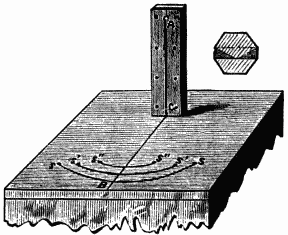
\includegraphics[width=0.8\textwidth]{images/fig01.png}
\label{fig01}
\end{figure}
the line of brightness on the stone at the time of solar noon
by a chronometer or a good watch carrying the time from
some accurate source. The best way of making\index{Meridian dial!method of constructing one} these
gnomons is to screw a pair of thin zinc or copper cheeks on
a cast iron upright piece, without attempting to make a
sufficiently narrow slit in the iron itself. It should have a
thick polygonal lump at the bottom screwing on to an iron
rod or `lewis' let into the stone, and lead or cement run
round it after it is set upright and as near the meridian as
possible. The octagon in the drawing shows the shape of
this base and the section across the middle of the gnomon.
I\index{Beckett, Sir E.!meridian dial} fixed the first of these,
without a chronometer, in the
garden of a vicarage near Cambridge in 1838, by the following
method; and as it was afterwards tested by Professor
Challis and found as right as can be practically
observed, the method
may be safely followed.
$\mathrm{AC}$ is the slit,
which I have generally
had about $9$
inches high. About
an hour before noon,
on a fine day in
summer, when the
shadow is short
enough to lie within
the slab, mark with
a pencil where the
top of the bright
line, or centre of the
little hole at $\mathrm{A}$ falls, say at $\mathrm{S}$, and draw the arc of a circle
$\mathrm{S}s$ with radius $\mathrm{CS}$\@. Mark again two other spots, $\mathrm{S}^\prime$ and $\mathrm{S}^{\prime\prime}$,
at about $11.15$ and $11.30$~\textsc{a.m.}, and draw the corresponding
arcs, $\mathrm{S}^\prime s^\prime$ and $\mathrm{S}^{\prime\prime}s^{\prime\prime}$.
Then watch for the times when the
end of the bright line again falls on each of the three circles,
%-----File: 029.png---------------------------------------------
%-----Folio: 14-------------------------------------------------
and mark the places $s$~$s^\prime$~$s^{\prime\prime}$. Bisect all the arcs, and if a
straight line $\mathrm{CB}$ will run through all the bisections, you
may be pretty sure that is the true meridian; if not, some
mistake has been made, and you must try again another day.

As you will probably begin to fix the slab and gnomon by
the compass, it may be as well to mention that the apparent
magnetic north in England is about $18^\circ$ west of real north
at present; for it decreases now slightly with time, and is
different in different parts of the world.

\begin{figure}[htb]
\centering
\hypertarget{fig2}{\caption{\sc The Dipleidoscope}}
\setlength{\unitlength}{0.7cm}
\begin{picture}(8,18.5)(-4,0)
%Thick triangle
\multiput(-4,6)(0,0.025){11}{\line(1,0){8}}
\multiput(0,0)(0.025,-0.016666){10}{\line(2,3){4}}
\multiput(0,0)(-0.025,-0.016666){10}{\line(-2,3){4}}
%Lines
\put(1,1.5){\line(-1,4){4.25}}
\put(-2,3){\line(1,6){2.583333}}
\put(-2,3){\line(2,-1){3}}
\put(-0.1875,6.25){\line(1,4){3.0625}}
%labels
\put(0,0.3){\makebox(0,0)[b]{A}}
\put(-3.6,5.8){\makebox(0,0)[tl]{B}}
\put(3.6,5.8){\makebox(0,0)[tr]{C}}
\put(1.1,1.8){\makebox(0,0)[b]{$\beta$}}
\put(0.8,1.5){\makebox(0,0)[tr]{$\beta$}}
\put(-2.1,3.2){\makebox(0,0)[b]{$\gamma$}}
\put(-1.7,2.7){\makebox(0,0)[tl]{$\gamma$}}
\put(-3.5,18.5){\makebox(0,0)[t]{S}}
\put(1,18.5){\makebox(0,0)[t]{$\mathrm{R}_2$}}
\put(3.25,18.5){\makebox(0,0)[t]{$\mathrm{R}_1$}}
\put(-1.3,6.4){\makebox(0,0)[bl]{$\alpha$}}
\put(-1.7,5.9){\makebox(0,0)[tr]{$\alpha$}}
\put(-0.1875,6.7){\makebox(0,0)[b]{I}}
\put(0.5,6.4){\makebox(0,0)[b]{$\mathrm{A}-\delta$}}
\end{picture}
\label{fig02}
\end{figure}

\subsection[Dipleidoscope]{The Dipleidoscope}\ \label{subsec:Dipleidoscope}\index{Dipleidoscope,the|(}\index{Time, measures of!dipleidoscope}\markboth{THE DIPLEIDOSCOPE.}{MERIDIAN INSTRUMENTS.}is another meridian instrument,
which was invented by
the late Mr.~J.~M.~Bloxam\index{Bloxam!invented the dipleidoscope},
a barrister in
considerable practice
whose name I shall
have to mention again
with some clock inventions.
He took a patent
for it (long ago expired)
and assigned it to the
late Mr.~Dent, by whom
only they were made.
Its name, compounded
of $\delta\iota\pi\lambda\acute{o}o\varsigma$ double, $\epsilon\hat{\textrm{'}\!\!\iota}\delta o\varsigma$
an image, and $\sigma \kappa o\pi\acute{\epsilon}\epsilon\iota\nu$ to see, indicates the
principle of it; because
in all positions but one
you see a double image
of the sun reflected in
it; and if it is so fixed
that the single image---\textit{i.e.}\ the
coincidence of the two---occurs at solar noon, it
evidently becomes a meridian instrument. It has the advantage
also of reflecting the sun when it is just too cloudy
%-----File: 030.png---------------------------------------------
%-----Folio: 15-------------------------------------------------
%**Transcriber's note: A small part of the top right corner of this page was missing, so the word "see" is a guess.
\label{corner1}for a shadow to be distinct, and in fact you can only \correction{see}
it through darkened glass when the sun is bright.

The instrument consists of three small plates of glass put
together at their edges in a brass box about $2$~inches wide
and high, so as to form a hollow prism of any convenient
angle, no precision being necessary in this. $\mathrm{ABC}$ in \hyperlink{fig2}{this
figure} is the section of it at right angles to the axis of the
prism. The front glass $\mathrm{BC}$ is plain; the other two are
blackened behind to form reflectors. But though the front
glass is transparent, it also reflects, because there are dark
ones behind it. $\mathrm{SI}$ and $\mathrm{IR}_1$ are sections of the planes of
incidence and reflection of the sun's rays from the glass $\mathrm{BC}$,
those planes being all parallel to the axis of the prism,
which should be approximately parallel to the earth's axis.
Part of the rays passes through that glass, and is reflected
by glass $\mathrm{AC}$ to $\mathrm{AB}$, and again reflected there and
sent through $\mathrm{BC}$ to $\mathrm{R}_2$. Now let the angle of incidence,
and therefore of first reflection at I, be called $\mathrm{A}-\delta$ (A being
the angle between the two reflecting glasses), and let the other
angles be designated as in the figure. It requires no
mathematics beyond the knowledge that the three angles of
every triangle =~$180^\circ$, commonly called $\pi$ to see that the
angle $\beta = \pi-(\mathrm{C+A}-\delta)$ in the small triangle near $\mathrm{C}$;
and in the one near $\mathrm{A}$, $\gamma = \pi-(\mathrm{A} +\beta) = \mathrm{C}-\delta$; and in
the triangle near $\mathrm{B}$, $\alpha=\pi-(\mathrm{B} + \gamma)= \pi-(\mathrm{B + C} -\delta)
=\mathrm{A} + \delta$. That is to say, the angle $\alpha$, made by the plane of
emergence of the twice reflected rays with the front glass,
differs from that of the once reflected by $2\delta$. Therefore, if
the prism is so placed as to make $\delta=0$, which it will be if
the angle of incidence $=\mathrm{A}$, the twice reflected rays will
come out parallel to the once reflected, and the two images
of the sun will coincide. In fixing the instrument however,
we have nothing to do with the angles; but simply to adjust
it by trial with a chronometer (for it cannot be done without),
so that the images do coincide at solar noon.
%-----File: 031.png--------------------------------------------
%-----Folio: 16------------------------------------------------
%**Transcriber's note: A small part of the top left corner of this page was missing, so the words "They" and "where" are guesses.
\label{corner2}\correction{They} were at first made so as to be fixtures on the stone
\correction{where} they were set, and so they were always exposed to
the weather, and besides, if cemented in wrongly, they were
wrong for ever. To avoid both these evils, I suggested the
making of a brass plate to be fixed on the stone, with a
raised slip adjustable by screws, against which the instrument
is to be laid closely when used, but at other times it
may be kept in the house. Some of them are made
to turn on an axis parallel to the earth's axis, and then
they can be presented to the sun at other hours besides
noon, but only for the given latitude like a sun-dial. Some
are made adjustable for latitude also. They are moreover
made for star observations with the reflectors silvered instead
of blackened, on account of the greater feebleness of star
light. A table was published to be used with them,
showing the time of first and last contact of the two
images of the sun for every day in the year, as that
observable perhaps more accurately than the time of coincidence;
at any rate it gives three chances of observation
instead of one. But many people prefer my meridian slit.\index{Dipleidoscope,the|)}

\section{WATER AND SAND-CLOCKS.}\label{sec:WATER_AND_SAND-CLOCKS.}
\index{Time, measures of!water clocks}\index{Water clocks}\markboth{WATER AND SAND-CLOCKS.}{WATER CLOCKS.}
The earliest time-keeping \textit{machine} is the clepsydra\index{Clepsydr\ae{} of Greeks and Romans} or
water clock of the Greeks and Romans\index{Water clocks!used by the Greeks and Romans}, which was no doubt
made in various ways. Vitruvius mentions one made as a
water wheel, which would probably be very irregular. This
simplest in construction is a graduated cylindrical vessel
with a hole in the bottom, and this appears to have been the
most commonly used: but they must surely have discovered
that the water in that case by no means runs out
with uniform velocity, though they did not know, and some
of the modern writers on antiquities apparently do not either
that the velocity varies as the square root of the height of
the water above the hole. But if a trough is kept full by a
%-----File: 032.png--------------------------------------------
%-----Folio: 17------------------------------------------------
stream, and a hole made anywhere in it, the water will then
run uniformly into, and rise uniformly in, another cylindrical
vessel in which its height may be marked on the sides, if it
is of glass, or else by a floating index, and that will make a
very fair clock. I do not however find any notice of such a
one in books on Greek and Roman antiquities. Various
other forms of clepsydra are described in them, which it is
not worth while to copy here.

The case is different with \index{Sand clocks}\markboth{WATER AND SAND-CLOCKS.}{SAND CLOCKS.}\index{Time, measures of!sand clocks}sand. If a column of dry sand
ever so high stands over a small hole, the sand will run out
no faster than if it is a very moderate height, for the same
reason that a pile or cone of sand on a given base will stand
up to a certain height and angle only, which depends on the
amount of friction between the particles. The angles of the
waist of an hour-glass ought to agree with that natural angle
of the sand in order that it may run out uniformly to the end---if
that is of any consequence, which it hardly is for the
boiling of eggs, or even for the old use of limiting the length
of sermons; which object might sometimes be advantageously
accomplished now by a descending sounding-board, or as
sounding-boards are gone out of fashion, by a pulpit bottom
or `drop' let down by clock work after $25$~minutes.

The burning of graduated candles\index{Candles graduated, for marking time}\index{Time, measures of!graduated candles} was another mode of
marking time, and if the candles were of wax, as they
probably were, and sheltered from wind, and the wicks
uniform throughout, the measure would be accurate enough
for any purpose for which it was likely to be used. The
consumption of oil in a lamp might also be marked and used
in the same way.

This seems the proper place to notice a genuine water
clock, invented and used by Lord \index{Rosse, Lord, his water clock}\index{Water clocks!Lord Rosse's}Rosse for the important
purpose of driving an equatorial telescope\index{Telescope-driving clocks} so as to keep it
pointed to a star, against the earth's rotation, for which
there are various contrivances. It is described in the R.A.S.\ \textit{Monthly Notices},
vol.~xxvi., and the principle of it is that the
%-----File: 033.png--------------------------------------------
%-----Folio: 18------------------------------------------------
water is let out slowly from a box by an india rubber tube
carried by a float, so that its mouth is always at the same
small depth below the surface of the water; and as the
pressure depends only on that depth the outflow is uniform
and the descent of the float with it, and that has a cord attached
to it, and at the other end attached to the wheel which
drives the telescope. The great equatorial at Greenwich\index{Water clocks!the one at Greenwich} is
driven by another kind of water clock, which will be notified
farther on, as it is combined with a revolving pendulum, and
we will now proceed to what are properly called

\section{CLOCKS.}\label{sec:CLOCKS.}
\markboth{HISTORY OF CLOCKS.}{HISTORY OF CLOCKS.}
The invention\index{Clocks!invention of} of clocks driven by a weight has been
generally attributed to Pacificus, Archdeacon of Verona, in
the ninth century; and also to Gerbert, afterwards Pope
Silvester II., who made a clock at Magdeburg in 996, when
he was an Archbishop. But there does not seem to be any
contemporary proof that either of these were weight clocks;
nor is it certain that Gerbert's was a clock at all; for it is
described by an old writer quoted in Beckmann's `History of
Inventions' (4th ed.~1846) thus:---`Magdeburg horological
fecit, illud recte constituens considerate per fistulam stella
nautarum duce'---\textit{i.e.}\ `he made a time-piece at Magdeburg,
setting it by looking at the pole-star through a tube.' Beckmann
thought William, Abbot of Hirshaw in the eleventh
century, had the best claim to the invention; of whom it was
said, `Naturale horologium ad exemplum c\oe lestis hemisph\oe rii
excogitavit;' and soon after, certain monks had the
duty `horologium dirigere et temperare, et signa pulsare;'
which however looks rather like their directing the clock
than the clock them, or as they say at sea, `\textit{making it} ten
o'clock,' rather than learning from the clock that it is so.

But he also says that in those times the day and the
night were each divided into twelve hours, between sunset
%-----File: 034.png--------------------------------------------
%-----Folio: 19------------------------------------------------
and sunrise; and if so, such hours could not be shown by
any clocks; for we may be sure that no clocks of those
days were able to adapt themselves to hours of such varying
length. And all this seems to me very insufficient evidence
of the existence of clocks, as we now understand the word;
which, by the way, appears not to have driven out the older
word `horologe,' until the time of Henry VIII., having been
long  used for a bell (cloche).

But it may be safely concluded from the various allusions
to horologia, and to their striking  spontaneously, in the
twelfth  century, that genuine clocks had been invented
before then, though there is no surviving description of the
construction of any clock until the thirteenth century, when
it appears that a certain `horologium' was sent by the Sultan
of Egypt in 1232 to the Emperor Frederic II\@. `It resembled
internally a celestial globe in which the sun, moon, and
planets moved, \textit{being impelled by weights and wheels,} so that
they pointed out the hour, day and night, with certainty.'
The oldest clock mentioned in  England\index{Clocks!ancient clocks in England}\label{early} is that which
was put up in a former clock-tower of Westminster, with
some great bells, in 1288, out of a fine imposed on a corrupt
Lord Chief Justice, of which a memorial survived near the
same spot in a sun-dial which stood on a house in Palace
Yard, pulled down within my time, with the inscription
\textit{`Discite justitiam moniti.'} In 1292 a clock is mentioned in
Canterbury Cathedral, costing \pounds 30; and the old striking
part of the original one in Exeter Cathedral was at work not
long ago, and perhaps is still, though the going part had
been replaced; and the same at Peterborough, probably of
about the same date. That of Glastonbury Abbey, afterwards
at Wells Cathedral, dated 1325, is now in the South
Kensington Museum, going. One by Richard Wallingford,
Abbot of St.~Albans, made in 1326, is said to have been
such as there was not in all Europe, showing various
astronomical phenomena. There was also one at Dover
%-----File: 035.png--------------------------------------------
%-----Folio: 20------------------------------------------------
Castle, with the date 1348 on it. That also was exhibited
going in 1876.

\markboth{OLD CLOCKS.}{OLD CLOCKS.}A description and picture of the clock made by Henry de
Vick for Charles~V.\ of France in 1370 may be seen in old
editions of the \textit{Encyclop\ae dia Britannica,} whether authentic
or made up from some other I do not know. I did not
think it worth repeating in the eighth edition, for which I
wrote the article on clocks\index{Beckett, Sir E.!on `Clocks' \&c., in the \textit{Encyclop\ae dia Britannica}}. It\index{Clocks!construction of} was very like our common
clocks now, except that it had only an hour hand, and a
vibrating balance (but no  balance  spring) instead of a
pendulum. It is impossible that such a clock could go well,
and it seems strange that the apparently simpler contrivance
of a pendulum should not have come till four centuries
after clocks were first invented; and yet that is the
general tradition. I suppose therefore that the pendulum
in the old Peterborough, and Exeter, and other church
clocks were added long after their original construction.
Those clocks were wound up by long spikes or handles
sticking out of the wooden barrel over which the rope goes
which carries the weight. In many old church clocks the
weight is only a large stone. It is not until quite modern
times that church clocks had minute hands besides the hour
ones, but in other respects there is surprisingly little difference
in principle between the oldest of these machines and
most turret clocks of the present day.

The going part of a clock is, and always has been, nothing
but a train\index{Wheels for clocks!train of}\markboth{CLOCK TRAIN.}{CLOCK TRAIN.} of some number of wheels and pinions, of which
one turns in $12$~hours, and another in $1$~hour, if there is a
minute hand. The first, or slowest, or `great' wheel, is
turned by a weight hanging by a rope wound round a barrel
on that wheel's axis\index{Arbors, or axes, of wheels}, or \textit{arbor,}
as it is called in clock-making;
and the last or quickest wheel drives a fan-fly, or a fly-wheel,
or a pair of vibrating arms, called a `balance,' or a pendulum,
to regulate the velocity of the train. A spring clock is
merely a compound of a large watch and a common clock.
%-----File: 036.png--------------------------------------------
%-----Folio: 21------------------------------------------------
\begin{figure}[htb]
\centering
\caption{\sc Pinions}
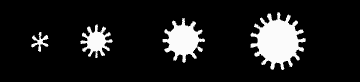
\includegraphics[width=\textwidth]{images/fig03.png}
\label{fig03}
\end{figure}

Any one who has looked at the inside of a clock---and it is
useless to read this book until you have---knows it consists
of a few\index{Train of wheels!in clocks} large wheels with a good many teeth, and that
the teeth of every large wheel, except the highest, are
engaged in or drive some much smaller
wheels fixed on the axes or arbors of all the large ones
except the largest. These small wheels are called pinions\index{Pinions of clocks}\label{pivots},
and their teeth are called `leaves' for distinction. This
figure~\ref{fig03} shows a set of pinions of from $6$ to $16$ leaves,
the lowest and the highest numbers used. It also
shows the kind of steel plate which is used
for drawing \textit{pinion wire}. For it is cheaper to make
the arbors of such wire, turning off the projections
all along the arbor except where they form the pinion itself,
than to cut the pinions out of the solid. But they are not
so good as cut ones, and I believe are not used in
the best clocks.

\begin{figure}[htb]
\centering
\caption{\sc Common Clock Train}
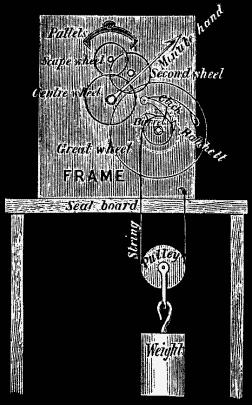
\includegraphics[width=252pt]{images/fig04.png}\index{Train of wheels!in clocks}\markboth{COMMON TRAIN.}{COMMON TRAIN.}
\label{fig04}
\end{figure}

The largest wheel in the train, which is called `the great wheel,'
\textit{appears} to be stuck on the end of the barrel which
carries the string and
%-----File: 037.png--------------------------------------------
%-----Folio: 22------------------------------------------------
the weight attached to it---whether with a moving pulley or
not, does not signify as a matter of principle, which is all we
are considering at present. The only effect of the pulley\index{Pulleys} in
to take a double string of twice the length of a single one in
the same clock case, which enables a larger barrel to be
used and also prevents the string from untwisting.

But if the great wheel were really fixed to the barrel there
could be no winding up, except by an endless chain contrivance,
which we need not now consider. Accordingly the
real arrangement is that the great wheel rides freely on the
arbor of the barrel, and is connected with it by a ratchet\index{Ratchet wheels}
and click; the ratchet being a saw-toothed wheel on the
end of the barrel, and the click being on the great wheel
with a spring to keep it in the ratchet teeth, which pass
under it in winding, but cannot return, except with the
great wheel itself. You will see a \hyperlink{fig29}{picture} of it under
`Maintaining Powers,' farther on in the book. And it is all
the same whether the barrel is turned in the old way by
spokes, or in the modern way by a key or `winder' put on
the squared end of the arbor; only in the former case the
barrel rides loose on the arbor, and in the latter is fixed
to it and the wheel rides loose. Consequently the weight
is always acting on the train, except at the time of winding;
and in all good clocks there are contrivances for keeping the
force on even then, called maintaining powers.

Now suppose the great wheel has \index{Wheels, numbers of teeth}$120$ teeth, and the
pinion which it drives has $10$; then if that pinion and its
arbor and the wheel stuck on to it turn in one hour, the
great wheel will evidently turn in $12$~hours. The wheel
which turns in an hour is called the centre wheel in house
clocks, because that arbor comes through to the centre of
the dial and carries the minute hand. Suppose that wheel
has $64$ teeth and drives a pinion of $8$; then that pinion and
the wheel on its arbor will turn in $8$~minutes; and if that has
$60$ teeth and drives another pinion of $8$, that pinion and
%-----File: 038.png---------------------------------------------
%-----Folio: 23-------------------------------------------------
arbor will turn in a minute, and the wheel on that arbor is
the scape-wheel, which drives the pendulum vibrating in a
second, as we shall see presently. Not that there is any
virtue in these particular numbers of teeth and leaves, or
that the pendulum need vibrate seconds; most church clock
pendulums are slower, and all short spring clock pendulums
are faster. All that is requisite theoretically is, that the
numbers of the teeth of all the wheels multiplied together,
and divided by the numbers of the leaves of all the pinions
multiplied together, should give the proper velocity-ratio
between the slowest wheel and the quickest. Thus, if the
scape wheel has to turn $60$ times as fast as the centre wheel,
and there is one between them, which may turn in any time,
the product of the teeth divided by that of the leaves must
= $60$, and subject to that, you may distribute the numbers
as you please---theoretically; but practically other considerations
come in, such as that the slower wheels must be larger
than the quicker ones, or they could not clear the arbors
below them; that if the leaves of the pinions are very
few they do not drive easily, and if they are many the
teeth must be many and small, and more expensive to cut,
and so forth; and the result is that, in the common long
house clocks the numbers are usually what I gave just now;
but in astronomical clocks or \textit{regulators} they are higher,
sometimes twice as much; in turret clocks they vary more,
according to circumstances, as will be seen hereafter.

The simplest of all the methods of regulating the velocity
of the train, and one which certainly existed before De Vick's
time, is the fan fly\label{fanfly},\markboth{FLIES AND FLY WHEELS.}{FLIES AND FLY WHEELS.} or a pair of arms with vanes which are
resisted by the air. I think it by no means improbable,
though it is never likely to be ascertained now, that some of
those earlier clocks were trains of wheels with a fly to regulate
their velocity, instead of a balance, which De Vick used in
his going part, though he had a fly in the striking part, as
the earlier English clocks have, and exactly as it is used to
%-----File: 039.png----------------------------------------------
%-----Folio: 24--------------------------------------------------
\index{Continuous motion clocks}%**Transcriber's note: I could not find this index reference in this page so have simply placed it at the page boundary.%
this day.    So long as the force and friction of the train are
uniform the velocity of the fly will be uniform, as the variation
of density of the air is too small to affect it materially;
and it should be observed, that a long fly with a rather slow
motion is less affected by variations of force than a short and
quick one; but as far more accurate methods are now used,
it is unnecessary to go further into this.

A fly wheel\index{Fly-wheel clocks, earliest}, which is either a wheel with a heavy rim or
a pair of weighted arms at right angles to the axis which
carries them, is another method; but not so good, because,
not  being  resisted by  the   air  nearly  so  much  as fans,
it is much more affected by a change of force, which in
clock work nearly always means a change of friction in the
train.     It acts simply by its moment of inertia, which is
constant, and therefore the velocity cannot be constant if
the force varies.    In fact there is theoretically no limit to
the velocity of a fly wheel driven by a weight, so long as
the weight can go on falling, though practically a terminal
velocity is soon reached, when the friction and the increasing
resistance of the air balance the force; but of course this
balance is disturbed  and the velocity changes as  soon as
the force varies.

\subsection[Conical Pendulum.]{Conical Pendulum.}\ \label{subsec:Conical_Pendulum.}\index{Conical pendulum}\index{Pendulum2@Pendulum!conical or revolving}\markboth{CONICAL PENDULUM.}{CONICAL PENDULUM.}A
pair of weighted arms attached
to   a   revolving   vertical   axis   by   horizontal   hinges, so
that they can fly farther out as they go, will regulate the
velocity more completely than a fly wheel or arms rigidly
fixed,   and   still  better if it has fans  attached to it, but
not  completely  enough to  keep  it  uniform  if the force
varies much.     They are like the `governor' of a  steam
engine in appearance, but no further; for the governor arms
work a lever which opens more or less of the throttle valve
of the steam pipe, according as the engine is going too slow
or too fast.    A single ball or pair of balls hung in this way
and driven by a clock train form what is called a \textit{conical
pendulum}, because each arm describes a cone, and the time
%-----File: 040.png----------------------------------------------
%-----Folio: 25--------------------------------------------------
of its revolution may easily be determined as follows, except
so far as it is affected by friction and resistance of air:---

Let\label{lg} $l$ be the length of each arm, and $\phi$ the angle at which
it happens to be inclined to the vertical axis, which of course
depends on the rate of revolution or angular velocity, which
is usually called $\omega$; then the centrifugal force of each ball
$=\omega^2 l\sin\phi$; and as that is the force which keeps the balls
away from the vertical, it must balance the force which
draws them to it, which is $g \tan\phi$ ($g$ being the usual symbol
for the force of gravity, or twice the number of feet which a
body falls in the first second of time, and $g$ in this latitude
is $32.2$); therefore $\omega$ or the angular space moved over by
the arms in one
\begin{wrapfigure}{o}{111pt}
\centering\index{Pendulum2@Pendulum!conical or revolving}
\caption{\sc Revolving Pendulum}
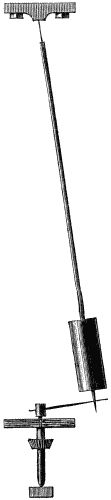
\includegraphics[height=500pt]{images/fig05.png}
\label{fig05}
\end{wrapfigure}
second $=\surd{\frac{g}{l\cos \phi}}$,   and  the  time  of
a complete   revolution   through   $360^\circ$   or   $2\pi$, is $\frac{2\pi}{\omega} =
2 \pi \surd{\frac{l\cos \phi}{g}}$.
If you wish to know what that means in
figures, you must express $l$ in feet, as $g$ is, and write the
numerical value $3.14159$ for $\pi$, and take the numerical
value of $\cos \phi$ from a table of sines and cosines; and the
result, after extracting the square root and dividing, is the
number of seconds in which the revolution is performed.
We shall see hereafter that it is just so much less than the
time of a common vibrating pendulum of the same length as
$\surd{\cos \theta}$ is less than $1$. And as the cosine varies least when
an angle is small, a clock of this kind will go better when
the length of the arms and the weight of the balls are such
that they make only a small angle with the axis when the
clock weight is driving them. But again it must be
remembered that these results are very much modified in
actual working by the resistance of the air, which acts
more strongly on the balls as they fly farther out, and
thereby tends to regulate  the velocity, as it does with a
fan fly.
%-----File: 041.png----------------------------------------------
%-----Folio: 26--------------------------------------------------

A clock of this kind is often used\index{Conical pendulum!its uses} to turn the reflectors or
coloured lenses of revolving lighthouses\index{Light-house clocks}, and also for the
more accurate purpose of driving large equatorial telescopes\index{Telescope-driving clocks},
to keep them pointed to a star notwithstanding the revolution
of the earth. For the earth does not move by jerks, as a
clock with a vibrating pendulum and escapement necessarily
does. A revolving pendulum\index{Pendulum2@Pendulum!conical or revolving} alone will not do without some
contrivance to equalise the force upon it, or to check the
pendulum itself by friction.

The  simplest form of it is setting the revolving balls
within a conical ring, which they can graze slightly, and it
is better if they are furnished with slight grazing springs.
And if the cone is also made raisable by a handle within
reach of the observer, so that he can regulate the friction,
probably this is enough in all ordinary cases.

But for telescopes of great importance superior contrivances
are used. The chronograph at Greenwich\index{Chronograph at Greenwich}, which
drives a barrel covered with paper, on which the times of
various observations are pricked by galvanic communication
from the observers, is an ordinary clock with a revolving
pendulum, driven by an arm which also carries round a kind
of spade, dipped a little into an annular trough of water;
and the farther out the pendulum swings the deeper it pushes
the spade into the water, by a simple lever arrangement
which can easily be imagined.

The great equatorial\index{Equatorial telescope at Greenwich, its driving apparatus}\index{Greenwich!equatorial driving clock} telescope there has a similar pendulum
and trough; but besides that, the clock is itself driven by a
`Barker's mill\label{barker},' or a pair of revolving horizontal arms on a
vertical axis, all hollow and receiving water at the top of
the axis.    The arms have holes near their ends, on opposite
sides, and the water flowing out there drives the arms the
other way.    The pendulum also works a throttle valve as
the governor of a steam engine does, and so regulates the
flow of water through the mill.

A revolving pendulum may be hung by a single wire, as
%-----File: 042.png----------------------------------------------
%-----Folio: 27--------------------------------------------------
there is no tendency to twist, and
they are so made in bedroom clocks,
which have the advantage of being
silent. But it is  difficult  to  get
a wire strong enough for a heavy
pendulum which would not also be
too stiff.    The Greenwich ones are
hung by a kind of universal joint,
made of two pairs of suspension
springs in stirrups, set across each
other, one turned upwards and the
other downwards, with a cross between.

We shall have to notice afterwards
some other clocks for this purpose,
in which a revolving continuous\index{Greenwich!revolving pendulum}
movement is combined with a vibrating
pendulum and escapement; but
I must describe escapements first.

It is perhaps worth mentioning
that any point in a wheel revolving
uniformly has always the same velocity
in a horizontal direction as some
point in a pendulum which makes
a double vibration in the same time
as the wheel revolves; and therefore,
theoretically, a constant motion of
a clock-train might be got by connecting
some point in a $1$~sec.\ pendulum
with a pin in a small disc
revolving in $2$~seconds, by a rod so
long as to be practically horizontal.
But it would probably be impracticable
to keep the force constant
enough to give just proper impulse
%-----File: 043.png---------------------------------------------
%-----Folio: 28-------------------------------------------------
to the pendulum; and if too much was given, there would
be a jerk at the end of every beat, and if too little, the
pendulum and the clock would stop.

\section{BALANCE-WHEEL ESCAPEMENTS.}\markboth{BALANCE-WHEEL ESCAPEMENTS.}{BALANCE-WHEEL ESCAPEMENTS.}\label{sec:BALANCE-WHEEL_ESCAPEMENTS.}\index{Balance-wheel clock escapements}\index{Escapements of clocks}

Before we go into the theory of pendulums we should
notice the one other mode of regulating the motion of a
clock-train which existed long before pendulums were
applied. The earliest
escapement of which
there is any known
description is that
which De Vick's\index{De~Vick's clock escapement} clock
had, and which is
called the \label{crown}crown-wheel
escapement. The object
of that, as of all
the later escapements,
was to let a tooth of
the quickest wheel in
the train escape past
some stops called
\textit{pallets}\index{Pallets} at every vibration
of the balance,
and that wheel is
thence called the
scape-wheel, and a
crown-wheel from its
shape. The pallets $\mathrm{A}$,
$\mathrm{B}$, in fig.~\ref{fig06}, are pieces
\begin{figure}[htbp]
\centering
\caption{\sc Balance Wheel Escapement}
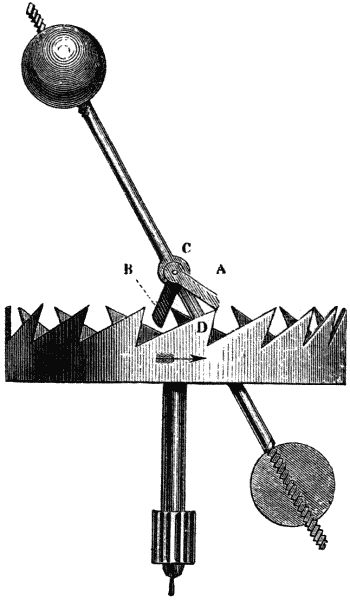
\includegraphics[height=0.7\textheight]{images/fig06.png}
\label{fig06}
\end{figure}
of steel fixed to the
axis or arbor of the
balance $\mathrm{C}$ in planes at
right angles to each
other, one of them set so as to be pushed one way by
%-----File: 044.png---------------------------------------------
%-----Folio: 29-------------------------------------------------
the front teeth $\mathrm{D}$ of the wheel, and the other the other way
by the back teeth. As one tooth escapes past its pallet, the
other pallet is in a position to receive and stop the opposite
tooth. But as the balance has then acquired a swing in the
direction in which it has been pushed by the escaping tooth,
it does not stop immediately, but swings a little farther and
so drives the wheel back again a little, producing what is
called the recoil. This is just the same as the old `vertical'\index{Vertical watch escapement}
watch escapement, which remained in use until a few years
ago, with this important exception, that the time of vibration
of a watch balance is regulated by a thin spiral spring fixed
to it and to the frame, whereas this had none, and so its
regulating power over the train depended solely on its
moment of inertia, and on its swinging farther for any
increase of force, which by no means makes it isochronous.

The same thing is still to be found in bottle-jacks\markboth{BOTTLE-JACK ESCAPEMENT.}{BOTTLE-JACK ESCAPEMENT.}\index{Bottle-jack escapement}; the
piece of meat to be roasted forms the balance, and the noise
at each change of its motion is the `ticking' of the escapement.
It is true the meat makes several turns for one tick,
while De Vick's balance made only half a turn, but that is
because there is a wheel on the pallet arbor in the jack,
worked by a pinion on the meat arbor, as in the rack lever
watch escapement; but otherwise the bottle-jack escapement
is precisely the same as in De Vick's clock, in which the
axis of the balance was vertical, and not horizontal as in
fig.~\ref{fig06}.

\section{PENDULUMS.}\label{sec:PENDULUMS.}\markboth{PENDULUMS.}{PENDULUMS.}

Pendulums, like many other things, may have been\index{Pendulums!invented}
invented several times over in different ages, or even in the
same. In an old edition of the \textit{Encyclop\ae dia Britannica} it
is said that `the ancient astronomers of the east employed
pendulums in measuring the times of their observations,
patiently counting their vibrations during the phases of an
eclipse or the transit of the stars, and renewing them by a
%-----File: 045.png---------------------------------------------
%-----Folio: 30-------------------------------------------------
little  push  of   the   finger   when   they  \correction{languished.} %**Transcriber's note: The top right corner of this page was missing, so the full-stop after "languished" is a guess.
\label{corner3}Gassendi,   Riccioli,   and   others,   in   more   recent times
followed their example.'    If so, it is plain that this knowledge
had itself languished and died, before the making of
what has long been called Galileo's discovery in the church
at Florence,  that  a  chandelier,   and  therefore  any other
pendulum, vibrated different arcs in the same time, provided
they were none of them large ones.    When we consider the
vast number of pendulums of various kinds that there are
swinging about the world, it certainly is difficult to imagine
that nobody ever made that observation before the sixteenth
century.    The application of it to the regulating of clocks
however is a  different thing, as that required invention as
well as observation.    To be sure, all that was needed was to
omit one of the weights in De~Vick's\index{De~Vick's clock escapement} balance, and set it in
a vertical instead of a horizontal plane, and it is strange
enough that this slight but valuable alteration should have
waited three centuries to be made.    It would then assume
this form (fig.~\ref{fig07}), which is the same as the other in all but
the position of the parts and the omission of one arm and
weight of the balance.    The bent end of the arm (called the
\textit{fork}\label{fork}) is substituted for a weight in this drawing, because it
was afterwards found better to hang the pendulum independently,
and connect it with that arm, called the \textit{crutch}, by
means of the fork.    But I have seen small clocks of the
last century, and even some modern French ones, with the
crutch itself made into a pendulum by merely putting a ball
at the end of it.

There seems no doubt however that the first person who
investigated and established the mathematical theory and
properties of the pendulum was Huyghens\index{Huyghens!theory of the pendulum}\label{huyghens}, the Dutch philosopher,
in the seventeenth century; but it seems equally
certain that the first pendulum clock was made for St.~Paul's
Church in Covent Garden, by Harris, a London clock-maker
in 1621, though the credit of the invention was claimed also
%-----File: 046.png--------------------------------------------
%-----Folio: 31------------------------------------------------
by Huyghens himself, and by Galileo's son, and Avicenna,
and the celebrated Dr.~Hooke\index{Hooke, inventor of the balance-spring of watches}, the undoubted inventor of
the balance spring of watches, and  the discoverer of its
theory.
\begin{figure}[htbp]
\centering
\caption{\sc Crown-Wheel Escapement}
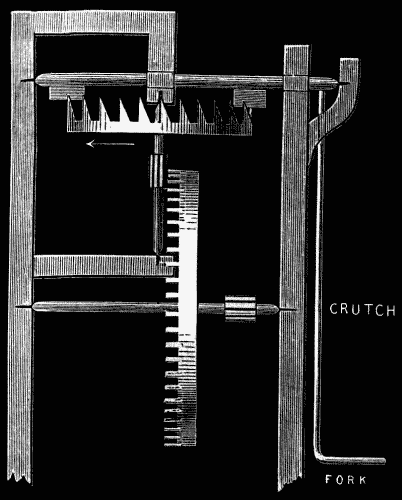
\includegraphics[width=0.9\textwidth]{images/fig07.png}\markright{CROWN-WHEEL ESCAPEMENT.}
\label{fig07}
\end{figure}
The main point of Huyghens's discovery seems at first sight
a long way off any connection with what we now understand
by a pendulum, viz., a weight or \textit{bob}\index{Bobs for pendulums}\index{Pendulum!bobs} at the bottom of a long
rod, which is hung by a string or a thin spring at the top,
and the bob therefore swinging in a circular arc, or something
very near it. For he proved that the curve in which
a bob hung by a string of insensible weight must move in
%-----File: 047.png--------------------------------------------
%-----Folio: 32------------------------------------------------
order to be isochronous in its vibrations, is \textit{not} a circle, but
a cycloid, or the curve traced out by a point in the rim of a
circle rolling upon a straight line, \textit{e.g.}, a nail in the tire of a
carriage wheel rolling on a smooth road, or $\mathrm{P}$ in circle
$\mathrm{DEP}$ rolling on $\mathrm{BGC}$ in fig.~\ref{fig08}; and he showed how a
certain other property of the cycloid might be made use of
to enable a pendulum bob to describe a cycloidal\index{Cycloidal!theory}\markright{CYCLOIDAL CHEEKS.} instead of
a circular arc. It is not worth while to fill these pages with
demonstrations which may be found in any mathematical
treatise on mechanics, especially as I must assume the reader
to have some of the knowledge which is only to be got from
such books, in order to understand the demonstrations if I
gave  them. Therefore we may as well begin at this
point, that a body moving by gravity in a cycloid (with
the curve downwards, as $\mathrm{BPFC}$ in fig.~\ref{fig08}) does describe
\begin{figure}[htbp]
\centering\index{Pendulums!cycloidal theory}
\caption{\sc Cycloidal Theory}
\setlength{\unitlength}{1.5cm}
\begin{picture}(6.283184,4.5)(0,-2.25)
\put(0,0){\line(1,0){6.283184}}
\put(3.141592,-2){\line(0,1){4}}
\qbezier(0,0)(0,-0.429204)(0.570796,-1)
\qbezier(0.570796,-1)(1.570796,-2)(3.141592,-2)
\qbezier(5.712388,-1)(4.712388,-2)(3.141592,-2)
\qbezier(6.283184,0)(6.283184,-0.429204)(5.712388,-1)
\qbezier(3.141592,2)(3.141592,1.570796)(3.712388,1)
\qbezier(3.712388,1)(4.712388,0)(6.283184,0)
\qbezier(2.570796,1)(1.570796,0)(0,0)
\qbezier(3.141592,2)(3.141592,1.570796)(2.570796,1)
\put(3.712388,1){\line(1,-1){2}}
\put(4.712388,0){\line(0,-1){2}}
\qbezier(4.712388,0)(5.126603,0)(5.419496,-0.292893)
\qbezier(5.419496,-0.292893)(5.712388,-0.585821)(5.712388,-1)
\qbezier(5.419496,-1.707107)(5.712388,-1.414179)(5.712388,-1)
\qbezier(4.712388,-2)(5.126603,-2)(5.419496,-1.707107)
\put(3.141592,2.1){\makebox(0,0)[b]{A}}
\put(0,0.1){\makebox(0,0)[b]{C}}
\put(6.283814,0.1){\makebox(0,0)[b]{B}}
\put(3.141592,-2.1){\makebox(0,0)[t]{F}}
\put(4.712388,0.1){\makebox(0,0)[b]{D}}
\put(4.712388,-2.1){\makebox(0,0)[t]{E}}
\put(5.762388,-1){\makebox(0,0)[tl]{P}}
\put(3.101592,-0.1){\makebox(0,0)[tr]{G}}
\end{picture}
\label{fig08}
\end{figure}
both large and small arcs  in the same time;  the reason
of which is that the force may be proved to be always in
proportion to the distance along the curve from its lowest point
point, $\mathrm{F}$.
%-----File: 048.png--------------------------------------------
%-----Folio: 33------------------------------------------------

But how is a pendulum bob, hung by a string or wire
from a fixed point, to be persuaded to describe a cycloid?\index{Pendulums!cycloidal theory|(}
It so happens that if a cycloid $\mathrm{BFC}$ is cut in two, and one
half $\mathrm{BF}$ removed as a solid with a convex edge to $\mathrm{AC}$
(making $\mathrm{AG=FG=DE}$), and the other half to $\mathrm{AB}$, the
end $\mathrm{P}$ of a string $=\mathrm{AF}$, fixed at $\mathrm{A}$, and moving between
those `cycloidal cheeks' will redescribe the old cycloid
$\mathrm{BFC}$\@. This is mathematically expressed  by saying that
the \textit{involute} of a cycloid is another equal cycloid, and therefore
also the \textit{evolute} is; the evolute being the cheeks, and the
involute the curve described from them: the proof of this
belongs of course to geometry, not mechanics, and is of no
consequence to us at present. Huyghens therefore proposed
to hang clock pendulums by a string or a thin spring between
cycloidal cheeks, and that was for some time thought a very
superior method of making clocks. I have no doubt there
are some still in existence, as I have seen them.

But after a time it was found that clocks went rather
worse with these cheeks\index{Cycloidal!cheeks useless}\label{cheeks} than without them; and then it
occurred to somebody that the cycloidal theory is only true
for what is called in mathematics a simple pendulum, or one
in which not only the bob, but the centre of the bob, is
alone supposed to have any weight; and of course there is
no such thing possible, for the rod must have some thickness,
or it is not stiff enough to work, or to be driven by the
clock, and if you make the bob very heavy, with the view of
rendering the weight of the rod insignificant, then the bob
itself must be large, and differs considerably in its mechanical
effect from a single imaginary heavy point at its centre. And
besides that, the spring or string cannot be made to act
against the cheeks without friction and other disturbing
causes; all which things are said to have been proved to
produce greater deviations from isochronism than a variation
of several degrees in the arc. Indeed we shall see hereafter
that the common clock escapements tend to produce an error
%-----File: 049.png--------------------------------------------
%-----Folio: 34------------------------------------------------
of their own, which the deviation from cycloidal vibration
(commonly called the \textit{circular error\index{Circular error of pendulum}) }is actually useful in
counteracting.

Nevertheless the cycloidal theory is valuable to this
extent: it shows why a common pendulum is very nearly
isochronous for different \textit{small} arcs; for the string $\mathrm{AP}$ will
evidently describe  very nearly the same curve near the
bottom $\mathrm{F}$, whether the cheeks are there or not: in other
words, a  bob vibrating in a small circular arc is almost
identical with one in a cycloidal arc described by a string of
the same length. The actual time of a circular vibration
cannot be calculated without the aid of the higher branches
of the integral calculus, and even then it can only be exhibited
in the form of a rather awkward series, which would
be little better than useless, except for small arcs; and for
them it is quite sufficient to take only the two first terms of
it.\index{Pendulums!cycloidal theory|)} The whole calculation may be found in \textit{Pratt's Mechanics,
} or in the 8th edition of the \textit{Encyclop\ae dia Britannica,} under
article \textit{Pendulum.} The first term is simply the expression
for a cycloidal vibration, $t=\pi\surd{\frac{l}{g}}$ the letters of which
I have already explained at p.~\pageref{lg}, for the conical pendulum,
whose time of vibration you now see is less than that of a
plane pendulum of the same length in the proportion of
$\surd$cosine of the angle which the conical one makes with the
vertical axis.

\subsection[Circular error.]{Circular error.}\label{subsec:Circular_error.}\markright{CIRCULAR ERROR.}\index{Circular error of pendulum}\index{Pendulums!circular error of}---The next term in the series (omitting
all the later ones which are still smaller) constitutes the
circular error $\mathrm{K}$, or the excess of the time of vibration in a
circular arc over that in the cycloidal one belonging to the
same length of pendulum; and it is accurate enough for all
practical purposes to say that $\mathrm{K}=\pi\frac{a^2}{16}\surd{\frac{l}{g}}$; and therefore
for a whole day, $\mathrm{K}= 5400 a^2$ in seconds, whatever the
length of the pendulum is; the amount of which you may
%-----File: 050.png--------------------------------------------
%-----Folio: 35------------------------------------------------
easily calculate from the fact that if $a=2^\circ$, as usual in
clocks its numerical value is $.035$, and therefore $\mathrm{K}$ = about
$6$~seconds. But this is more than what is called the circular
error in a clock pendulum; for we need not care what is the
difference between the time of a cycloidal arc\index{Arcs of vibration in clocks} and the actual
circular arc which the pendulum describes, but only between
two small circular arcs, $a$ and $a_1$, as the pendulum is
likely to describe in different states of the clock. This
quantity, which we may call $\Delta\mathrm{K}$, is only $5400 (a^2 \sim a_1^2)$;
and if we assume the larger of the two arcs to be as much
$2\frac12^\circ$ and the smaller $2^\circ$, the circular error between them
will be rather less than $4$~seconds a day. This is a very large
variation of arc for a tolerably good clock, and when it is as
small as it generally is, the circular error may be expressed
by differentiating the expression $5400 a^2$, and we may say (so
long as both the arc and its variations are small, remember)
that $\Delta\mathrm{K}=10800a\,da$ ($da$ being the variation of the arc).
Thus if $a=2^\circ$ and $da=10^\prime$, $\Delta\mathrm{K}$ will be very nearly
$1$~second: \textit{i.e.}\ the clock will lose a second a day for such an
increase of the arc, independently of any other increase or
counteraction of the circular error, which may be produced
by the escapement at the same time.

For the common purpose of finding the length of a pendulum
to beat seconds, or any other required time, we need
not trouble ourselves with anything beyond the equation\label{maths}
$t=\pi\surd \frac{l}{g}$ in which $t$ is the number or fraction of seconds,
and $l$ is expressed in feet, because $g$ means $32.2$~feet (in this
latitude), and $\pi$ is $3.1416$ or the numerical value of $180^\circ$.
Therefore in order that $t$ may be $1$~second, you will easily
find by a little calculation that $l$ must be $39.1393$~inches;
and having got that fixed, you may find the length of
pendulum for any other time of vibration very easily by
multiplying $39.14$~inches by the square of the ratio of the
%-----File: 051.png--------------------------------------------
%-----Folio: 36------------------------------------------------
intended time to $1$~second. But to save trouble I will put
down a few of the lengths\index{Pendulums!lengths of}, omitting small fractions.

\begin{table}[!hbtp]
\centering\index{Pendulums!lengths of}\label{lengths}\markboth{LENGTHS OF PENDULUMS.}{LENGTHS OF PENDULUMS.}
\begin{tabular}{r@{}lrl|cr@{}l}
\multicolumn{2}{c}{\sc seconds}&\sc ft. &\multicolumn{1}{c|}{\sc in.}&\sc seconds.&\multicolumn{2}{c}{\sc inches.}\\
\phantom{\sc sec}$4$&&$52$  &$2$           &$1\frac14$            &\phantom{\sc in}$61$& \\[1ex]
$3$   &           &$29$     &$4$         &$1$\phantom{$\frac14$}&$39$ &$.14$ \\[1ex]
$2$   &$\frac12$  &$20$     &$5$         &$\frac34$             &$22$ &      \\[1ex]
$2$   &           &$13$     &$0\frac12$  &$\frac23$             &$17$ &$.4 $ \\[1ex]
$1$   &$\frac12$  &$7 $     &$4$         &$\frac12$             &$9 $ &$.78$
\end{tabular}
\end{table}

These seconds, and the second used as the unit of time in
all mathematical formulas, are seconds of mean time; and as
a sidereal day is shorter than a mean one in the ratio of
$.99727$ to $1$, a sidereal pendulum must be shorter than a
mean one in the square of that ratio, which makes the
sidereal seconds pendulum at Greenwich $38.87$~inches. I
have met with persons who could not understand how an
increasing gravity can make pendulums go faster; and
others, with a little mathematical knowledge, think that the
force varying as the distance from zero (in small arcs) is
opposite to the fundamental law of gravity varying inversely
as the square of the distance. The answer to the second of
these is, that the zero, or middle, or lowest position of a
pendulum is not an attracting body like the earth (which
attracts as if it were all condensed into its centre); and the
tendency towards zero is only a mathematical consequence of
that law of gravity. The stronger the tendency to zero, or the
stronger gravity is, the faster the pendulum will evidently
fall; and the sooner gravity will bring it again to rest in rising.
The time of rising always = the time of falling, under any
force which is equal at equal heights during the rise and fall.

\subsection[Centre of oscillation.]{Centre of oscillation.}\label{subsec:Centre_of_oscillation.}\index{Centre of oscillation of pendulums}\index{Oscillation, centre of}\index{Pendulums!centre of oscillation of}---It must be remembered that
these are only the theoretical lengths of \textit{simple pendulums}
with all the weight concentrated in the centre of the bob, and
that this theoretical length by no means coincides with the
actual length down to the centre of gravity\index{Pendulums!relation to gravity} of the pendulum,
but is always longer. This length may properly be called
%-----File: 052.png-----------------------------------------------
%-----Folio: 37---------------------------------------------------
the \index{Radius of oscillation of pendulums}\textit{radius of oscillation,}\markboth{RADIUS OF OSCILLATION.}{RADIUS OF OSCILLATION.} as the lower end of it is always
called the centre of oscillation; which is not a fixed point in
the body, like the centre of gravity, but a relative one, every
axis of suspension having a radius and centre of oscillation
of its own. It is not always a simple process to calculate
this length (which we may as well call $l$) for any given
pendulum as it requires either the integral calculus or some
rules deduced from it; but it will be easy to explain the
nature and meaning of the quantities on which it depends.
Let $m$ be the mass of each particle of the pendulum, which
in these calculations must not be confounded with the
weight, which is written $mg$ ($g$ being the force of gravity), $r$
the distance of $m$ from the axis of suspension, and $\mathrm{M}$ the
mass of the whole pendulum; then the radius of oscillation
$=$ the sum of each particle multiplied into the square of its
distance from the axis, divided by the sum of each particle
multiplied into its distance simply; that is to say,
$l = \frac{\sum m r^2}{\sum m r}$
($\sum$ being used to indicate this kind of summation, which can
only be performed by integration).

The numerator in this fraction is called the \textit{moment of
inertia} of the body with reference to that axis of suspension.
Of course there is some quantity $k^2$ which
$= \frac{\sum m r^2}{\mathrm{M}}$, and $k$
is then called the \textit{radius of gyration} for that axis, and $\mathrm{M}k^2$ is
obviously the moment of inertia again. In like manner
some quantity $h = \frac{\sum m r}{\mathrm{M}}$, and $h$ is then the distance of the
centre of gravity of the whole pendulum (not of the bob,
remember) from the same axis, which is easy enough to
find in bodies of the shape commonly used for pendulums.
It appears then that the effective length $l$ of a pendulum
always $= \frac{k^2}{h}$; and it is only when the rod is very thin and the
%-----File: 053.png-----------------------------------------------
%-----Folio: 38---------------------------------------------------
bob itself small but heavy, that $k$ and $h$ can be assumed to be
even approximately identical, and therefore both $= l$, as they
are in a simple pendulum. But it does conveniently happen
that the centre of oscillation in small pendulums of the usual
forms is generally near the centre of gravity of the bob, and
sometimes coincides with it, as we shall see.

This quantity $\mathrm{M}k^2$, the moment of inertia\label{moi}\markboth{MOMENT OF INERTIA.}{CENTRE OF OSCILLATION.}, always appears
in mathematical formulae as the resister of forces of rotation
or vibration on an axis, and of all disturbances of such forces
after they have set the body in motion, and therefore
we see at once why long and heavy pendulums are better
than short and light ones. There are a few other simple propositions
relating to the centre of oscillation and the theory
of pendulums, which it will be appropriate to notice here.

Draw a pendulum of any shape you like, supposed to be
vibrating in the plane of the paper, and call its centre of
suspension $\mathrm{S}$, and its centre of gravity $\mathrm{G}$, and the distance
between them $h$. All bodies have this property, that their
moment of inertia round any axis through $\mathrm{G}$ (which we call
$\mathrm{M}k_1^2$) is less than round any other axis parallel to that, and
we are not concerned with any but parallel axes; and
further, if the other axis is distant $h$ from the centre of
gravity, the $k^2$ round that new axis $= k_1^2 + h^2$. Therefore if $\mathrm{O}$,
somewhere below $\mathrm{G}$, is the centre of oscillation corresponding
to $\mathrm{S}$, $l$ or $\mathrm{SO} = \frac{k_1^2+h^2}{h}$; and $l-h$, or
$\mathrm{GO} = \frac{k_1^2}{SG}$; or the
centres of suspension and of oscillation are \label{reciprocal}reciprocal. In
fact, if the pendulum is wide enough, you may draw two
circles round $\mathrm{G}$ with radii $\mathrm{GS}$ and $\mathrm{GO}$, and if you stick an
axis through the pendulum, at right angles to the same plane
of vibration, anywhere in either of those two circles, it will
vibrate in the same time as on the original $\mathrm{S}$\@. Consequently,
if you construct a pendulum (symmetrical on both
sides of its middle plane of vibration, to prevent it swinging
with a twist) with one fixed axis $\mathrm{S}$, and another adjustable
%-----File: 054.png----------------------------------------------
%-----Folio: 39--------------------------------------------------
one for $\mathrm{O}$, and a movable weight to adjust the time by, you
can make it vibrate in the same time on both axes; and by
adjusting the movable weight also, the pendulum can be
made to agree with the vibrations  of a clock pendulum
which is beating seconds; and then the distance between $\mathrm{S}$
and $\mathrm{O}$, or the two knife edges which represent them, being
measured, we shall know that that is the length of the
simple seconds pendulum. It has also been proved that if
round axes are used instead of knife edges, the distance
between them (not their centres) equally represents the
radius of oscillation, provided the axes roll on a plane.

If all the standard \index{Pendulums!standard lengths}\label{standard}\markboth{PENDULUMS.}{PENDULUMS.}yard measures in the kingdom should
ever be lost, they could only be restored by this process,
according to an Act of Parliament, 5 Geo.~IV.~c.~74, which
declared that a yard is $\frac{36}{39.1393}$ of the length of the pendulum
which vibrates mean seconds in London at the level of the
sea, in a vacuum. The force of gravity decreases so much
towards the equator that an English pendulum would lose $2\frac14$
minutes a day there. The following rule for the length
of the seconds pendulum in any latitude has been deduced
from observation, near enough for all practical purposes:
$l = (1-.0027 \cos 2 \mbox{ lat.})\,39.1156$~inches; that number of
inches being the length of the pendulum at lat.~$45^\circ$. When
the latitude is more than $45^\circ$, $\cos 2 \mbox{ lat.}$ becomes $-$, and
so $l$ exceeds its length at $45^\circ$, as of course it ought to do.
Another still simpler formula is $l = 39.017$ [the length of a
seconds pendulum at the equator] $+\, .2 \sin^2$ of latitude.

That Act however has been repealed, and some standard
weights and measures are deposited in various public places
under an Act of 18 \& 19 Vic.~c.~72. The late Astronomer
Royal provided a set, open to anybody, at the Observatory
gate. But if they all happened to be destroyed, new ones could
be made from the old pendulum ratio. Indeed Mr.~Johnson
of Wilmington Square had one ready for that calamity.    A
%-----File: 055.png-----------------------------------------------
%-----Folio: 40---------------------------------------------------
simple pendulum $36$~in.\ long would vibrate in a time which
is to $1$s.\ as $36^2$ to $39.14^2$, or $.846$ of a second, or $70.92$ times
in a minute; and he has made a clock with a reversible
pendulum vibrating in that time, and consequently $36$~inches
between the two knife edges.

The length of a seconds pendulum so nearly resembles the
French \index{Metre, the French, a bad measure}\label{metre}\markboth{BADNESS OF THE FRENCH METRE.}{BADNESS OF THE FRENCH METRE.}metre of $39.371$~in., that some persons may fancy
that that most ridiculous and mischievous revolutionary
measure had an origin even as rational as being the length
of a seconds pendulum in some latitude. But it has not.
It was intended to be the $40$ millionth part of a meridian of
the earth---about as rational a standard as if we enacted that
the yard should be the $420$ millionth of the mean distance of
the moon, which it is very nearly; and astronomers know
the moon's distance within a less fraction than the difference
of the metre from what it pretends to be, but is not.\footnote{%
See the essay `On Celestial Weights and Measures,' in Sir J.~Herschel's
\textit{Familiar Lectures,} condemning the metre strongly.
} Yet
there are people who want to force on all the world this
absurd, inconvenient, and useless measure, invented by a
nation whose language is declining over all the world; while
the English language, with that standard of measures which
every man carries in his arms, his legs, and in his head, is
spreading over all the world, so that it will soon be the
only universal language to be found everywhere, if it is not
so already. Doctrinaires of this kind may cram penny-school
girls with French metres, and centimetres, and
kilograms; but our yard grew and will remain as the
natural standard of length until the stature of the human
race alters. For it is the length of a good stride of a man
of what is generally considered the best height, and that
height is two such lengths, and so is the stretch of his arms,
and a yard is the natural length of his walking-stick. A
metre would be the yard of a nation of giants. With the
yard too goes the equally natural and still older measure of
%-----File: 056.png-----------------------------------------------
%-----Folio: 41---------------------------------------------------
a foot, which all nations had, with such small variations as
would occur in times when they had no scientific provisions
for preserving exact standards. Some great authorities
believe inches to have been the oldest measure of all; and
the Egyptian cubit\index{Cubit of Pyramid, and Jewish}\label{cubit}, which was unquestionably used in
building the Pyramids, from the many simple multiples of it
which occur there, confirmed by the discovery of one
accidentally built up in a wall at Thebes, was probably $20$
of their inches, being a little more than $20$ of ours; and
the `sacred cubit' of the Jews was $25$, according to Sir
Isaac Newton. Probably the authors of the new $25$~inch
to a mile Ordnance survey of England little thought that
they were reverting to that ancient standard. At the same
time, I do not accept the theory of the Scotch Astronomer
Royal,\footnote{%
See an amusing pamphlet on it by Mr.~F.~D.~Wackerbarth, and the
remarks on the Pyramid in my `Book on Building.' (Lockwood \& Co.)}
that the $25$~inch cubit was embodied in the
Pyramid dimensions, besides the one of $20.7$~inches, or
$20$ of some of the old continental inches. A variation of one
thousandth is practically nothing in unscientific ages, and
is less than the variation of many foot-rules now, and it is
singular that if our inch were a $1000$th longer, the earth's
polar axis would be just $500$ million inches.

\subsection[Short and slow pendulums.]{Short and slow pendulums.}\label{subsec:Short_and_slow_pendulums.}\index{Pendulums!short and slow}\markboth{SHORT AND SLOW PENDULUMS.}{SHORT AND SLOW PENDULUMS.}---There is a kind of
pendulum which is properly enough used in the instrument
called a \textit{metronome}\index{Metronome, the}, for counting the time in music lessons in
a way that requires no particular accuracy, and occasionally,
but very improperly, used for small clocks. It follows from
the propositions I have been explaining, that if a pendulum
with a heavy rod is set vibrating on an axis very little above
its c.g.\ it will vibrate slowly, like a scalebeam; and
consequently you may have a $2$~seconds pendulum in the
compass of a few inches. But even if the weight of it were
equal to that of a large pendulum, its regulating power, or
power to resist \label{resist}disturbance, would be very much less,
%-----File: 057.png-----------------------------------------------
%-----Folio: 42---------------------------------------------------
because that is measured by the moment of inertia $\mathrm{M}k^2$,
which is the sum of the weight of each particle $\times$ its distance$^2$
from the axis, and that of course must be small in a short
pendulum, though its time may be long if $h$ is very small.
The time of a metronome pendulum is adjusted by a small
sliding weight on the rod above the axis of vibration, the
bob being of course below it. Moving the weight up brings
the c.g.\ of the whole nearer to the axis, and also increases
the $\mathrm{M}l^2$ of the whole, and so in both ways makes it go
slower, and \textit{vice vers\^a}. It is kept going by a roughly made
watch movement and a common recoil escapement, such as
I shall describe presently for clocks.

\subsection[Shape of pendulums.]{Shape of pendulums.}\label{subsec:Shape_of_pendulums.}\index{Pendulums!shape of}\index{Shape!of pendulums}\markboth{SHAPE OF PENDULUMS.}{SHAPE OF PENDULUMS.}---Whatever the shape of a pendulum
is in other respects, it is essential that the back and
front should be alike both in weight and shape; or to speak
mathematically, that it should be symmetrical on each
side of the middle plane of its vibration, or it will \textit{wobble,}
and vary its time in some irregular and incalculable way.
It does not \correction{significantly} \label{correction3}%**Transcriber's note: The original reads "signify".
however, if one side of the bob is larger
than the other in the direction of vibration; but as that
would look ugly and the other does not, one never sees the
ugly but innocent deviation, but frequently the other; for
the pendulums of common clocks are often unsymmetrical
in the back and front, and are therefore bad ones, though
perhaps as good as the clocks they belong to. For this
reason the old fashioned lens-shaped bob, or the flat cheese
shape which some clockmakers use for church pendulums,
are not good ones, because it requires great care to fix them
with their own middle plane coinciding with the middle
of the rod. It is true that a lens moves through the air
with less resistance than any other shape; but then it
must be very large to be of the same weight as a sphere or a
thick cylinder with the axis vertical, and we shall see afterwards
that nearly all clock errors are inversely as the weight
(and length) of the pendulum. But there is a shape which
%-----File: 058.png-----------------------------------------------
%-----Folio: 43---------------------------------------------------
would probably be found to combine some of the advantages
of both though Baily's experiments (in \textit{Phil. Trans.} for
1932) showed some results which no one could have
foreseen; I mean a cylinder of elliptic section, or one having
the same horizontal section as a lens, but thicker; or of
the section formed by two arcs of a circle of $120^\circ$, which
would make the horizontal length and thickness as  $12\frac18$
to $7$~inches---a very convenient size for a large bob\index{Bobs for pendulums}\index{Pendulum!bobs} $13$~in.\ high;
which would weigh about $188$~lbs.\ in cast iron and
$288$ in lead, and is equal to a round cylinder of $8\frac14$~inches
diameter. But such figures are only approximate, the
weight depending on the density of the casting; and I have
neglected the hole for the rod, as that would be compensated
and more by the rod's own weight. A spherical bob is not so
good as this shape, because a slight error or looseness in the
hole would throw much more of the weight on one side and
increase the tendency to \textit{wobble}, a very serious defect. For
all practical purposes a cylinder is probably the best shape,
and is used now in all the best large clocks. I also
introduced the plan of making the top slightly domical, to
prevent bits of dirt resting on it, which would accelerate the
pendulum, as we shall see presently under `regulation.'

Bobs for large clocks are generally made of cast iron,
partly because it is cheaper than lead, and also because very
heavy lead bobs are liable to be bruised out of shape in
moving about before the pendulum is hung. But there can
be no doubt that lead is best, as its specific gravity is half as
much again as iron, and therefore it is less resisted by the
air, which we shall see afterwards affects pendulums by no
means insensibly. For the same reason it is a mistake to put
lead bobs in brass cases, as is usually done in `regulators' or
astronomical clocks, as it increases the bulk much more
than the weight. The lead looks very well japanned. It is
equally absurd to case lead weights in brass, though it does
no actual harm as it does in the bob.
%-----File: 059.png-----------------------------------------------
%-----Folio: 44---------------------------------------------------

\subsection[Suspension of pendulums.]{Suspension of pendulums.}\label{subsec:Suspension_of_pendulums.}\index{Pendulums!suspension}\index{Suspension of pendulums}\markboth{SUSPENSION OF PENDULUMS.}{SUSPENSION OF PENDULUMS.}---Pendulums
are generally suspended
by a spring, for the obvious reason
that they then swing without any
friction---except of the air\index{Air!resistance of to pendulum}. Some
French pendulums are still hung
by a string, but that has some
friction. The spring is not designed
to act with any force as a spring,
though it does very slightly, and
therefore is not at all analogous to
the balance spring of a watch, which
is thus the substitute for gravity.
The spring is enclosed in a slit, or
between two pieces called chops at
the top of the pendulum, which also
carry the rod, except in the American
clocks, where the wire itself is
flattened out into a spring. The top
of the spring is also riveted between
two smaller pieces in common clocks,
so as to make a lump which holds
up the spring in the cock, which is
a fixed piece with a slit in it
just wide enough to hold the
spring. In clocks of the higher
class the two upper chops are much
thicker and firmly screwed together,
and a large pin put through them,
\begin{wrapfigure}{o}{113pt}
\centering
\hypertarget{fig09}{\caption{\sc Suspension of Pendulums}}
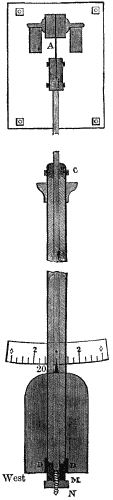
\includegraphics[height=500pt]{images/fig09.png}
\label{fig09}
\end{wrapfigure}
and the chops themselves go through
the cock tightly and are held up
by the pin which lies in $\mathrm{V}s$. This
will be better understood by \hyperlink{fig09}{this
picture} of a heavy pendulum and its
suspension. We are not concerned
%-----File: 060.png---------------------------------------------
%-----Folio: 45-------------------------------------------------
with the lower part just yet. The nearly square plate is
a cast iron plate bolted to the wall, out of which project
the two thick pieces on which the pin lies. The pin itself
is like a bolt with a tail projecting backwards through the
head, and the piece corresponding to the head, on the right
side in the figure, is the nut. The chops of the pendulum
itself are shown a little below, and the way I introduced
of making them for `regulator'\index{Regulation!of pendulums} or astronomical clock
pendulums which have the steel rod screwed into a solid
piece, is to file out a slit wide enough to hold the spring\index{Pendulum!springs}
and a piece of brass on each side of it, and the whole is
pinched together by a screw. You cannot cut a slit thin
enough for the spring  alone. This will be shown in the
figure of the four-legged gravity escapement hereafter.

A \label{fixing}perfectly firm\index{Pendulums!importance of firm fixing} suspension is essential to good performance
of any clock, and the heavier the pendulum the
firmer its support must be. It is well known that clocks
will influence\index{Clocks!influence one another} each other when fixed against a wooden wall,
however firm it may appear, and that one pendulum will
thus actually set another of equal length vibrating. Consequently
a free pendulum can be kept swinging from an
apparently immovable support which has an invisible
vibration or twist imparted to it by a clock below beating
in the same time. All good regulators have the pendulum
cock\index{Pendulum!cocks} screwed to the  back of the case, and that firmly
screwed to a strong wall; or, better still, the cock is cast
with a cast iron back or bracket which also  carries the
movement, and that is screwed directly to the wall, the
whole front of the  case lifting off. In the Westminster\index{Pendulum2@Pendulum!of the Westminster clock}
clock the pendulum cock is a large iron frame built in right
through the wall with a flange behind, and the cocks of
many other large clocks are fixed with bolts through the
wall. With a firm suspension the pendulum swings farther
than with a weak one, and we shall see afterwards that
(other things being equal) the errors of clocks  vary inversely
%-----File: 061.png---------------------------------------------
%-----Folio: 46-------------------------------------------------
as the square and sometimes as the cube of the
arc.

It is hardly necessary to say that the whole of the pendulum
suspension should be so adjusted that the bend of the
spring may be exactly opposite the pivot of the pallet arbor,
in order that the fork\index{Forks of pendulums} which embraces the pendulum, as
described at page~\pageref{fork}, may have as little friction as possible.
It must \label{shake}not however be tight, for the reason just now given,
viz.\ that no point in the pendulum describes quite a circle,
and the difference is sensible enough generally to stop the
clock if the fork fits the pendulum rod too tightly. It is
equally necessary that the plane of vibration of the pendulum
should be exactly at right angles to the pallet arbor, or
else there will be a sliding motion of the pendulum backwards
and forwards in the fork. But obvious as these
things are, they are all constantly neglected, especially in
large clocks, where the friction of all the parts is also the
greatest. The fork indeed is seldom left too tight, because
that mistake tells its own story directly; but, by way of
making up for it, it is very often so loose that you hear the
shake of it from one side to the other at every beat. There
ought to be a drop of oil there, as that is just enough
to keep a steady hold without either shake or tightness,
since oiled surfaces are not really in metallic contact.

In old church clocks a long pendulum was often \label{where}put for
convenience a good way off the clock, but so as to swing
in the same plane as the crutch\markboth{CONNECTION WITH CRUTCH.}{CONNECTION WITH CRUTCH.}, which is connected with it
by a light horizontal wooden bar, no heavier than an organ
`tracker.' The pendulum top too was often higher than the
pallet arbor, so that the pallets moved through a larger arc
than the pendulum. There is no advantage in that; but if
the pivots at the ends of the horizontal bar fit closely, there
may be less loss of power by `shake' than there generally
is between the fork and the pendulum. Indeed I have seen
old regulators made in that way, even with the pendulum in
%-----File: 062.png---------------------------------------------
%-----Folio: 47-------------------------------------------------
the usual place, by using two short horizontal arms thus,
$\mathrm{D}${\raisebox{.5ex}{\Huge{$<$}}\raisebox{.5ex}{\parbox[1em]{2ex}{$\mathrm{C}$\\[.5em]$\mathrm{P}$}}}, $\mathrm{C}$
being the pivot in the crutch, $\mathrm{P}$ the pivot
in the pendulum, and $\mathrm{D}$ the one at the junction of the two
arms $\mathrm{DC}$, $\mathrm{DP}$\@. But this is decidedly inferior to the other
plan of putting the pendulum on one side of the clock, since
that requires only two pivots instead of three, and there is
no twisting action on the pendulum. If the horizontal bar
were attached by slight springs it would be better still, for
there would then be neither shake nor friction, and the springs
would no more impede the action than the pendulum spring
does, for any moderate arc. There is yet in existence one
great London clock of the last century with fans on the pendulum
just above the bob (like the wings on the ankles of
Mercury) to prevent it swinging too far, and they are
actually placed obliquely, of which the effect of course is to
make it swing with a twist. The late Mr.~Vulliamy told me
he removed fans from the pendulum of the Horse Guards
clock. Sometimes heavy pendulums are hung by two
narrow springs instead of one broad and thin one, to secure
the vibration in the proper plane; but it is a bad plan,
because it is difficult to get the two springs equal in all
respects. The springs of `regulator' pendulums of $14$ or
$15$~lbs.\ are generally about $\frac12$ an inch broad and $2$~inches
long; I mean clear of the chops of course; that of the $6$~cwt.\
pendulum at Westminster is $3$~in.\ by $5$ and $\frac{1}{60}$~in.\ thick.

There should always be a degree plate\index{Degree plate for a pendulum}, with a pointer to
it on the pendulum wherever it can be most conveniently
seen. The length of $4^\circ$ on the plate is always $.07\times$ its
distance from the top of the pendulum; and as the only use
of the degree plate is to see that the pendulum keeps the
same arc, or to see how it varies, no very great accuracy is
required in the degrees.

\subsection[Pendulum springs.]{Pendulum springs.}\markboth{PENDULUM SPRINGS.}{PENDULUM SPRINGS.}\label{subsec:Pendulum_springs.}\index{Pendulums!springs of}---Various opinions have been propounded
on the proper strength for them, but none on any
%-----File: 063.png---------------------------------------------
%-----Folio: 48-------------------------------------------------
solid grounds, and some on altogether mistaken ideas of the
duty of the spring. Probably the thinner it is the better,
provided it is thick enough not to be bent too sharply or
strained by the weight of the pendulum. Every now and
then a clock is troubled with the disease of spring-breaking
over and over again. Sometimes this proceeds from the
lower edges of the upper chops being left sharp, which in
time cut the spring; and perhaps more frequently from
some unseen inequality in the fixing; and it is better to let
the pendulum hang at first with the lower chops a little
loose, and only to screw them up after the pendulum has got
a square bearing, and to take care not to put it out in
doing so. It is wonderful how much more trouble people
will take to do things wrong than would serve to do them
right, and it is almost incredible that some clock-makers
send out their best clocks with the lower edges of the upper
chops not horizontal but rounded into a circular arc.
The slightest reflection would show anybody that springs so
fixed must tend to `buckle,' or bend not in a straight line,
at every vibration. And others make the upper chops,
which have the strain of vibration, thinner and weaker than
the lower ones which have no strain. There should always
be a block of wood close under the bob of a heavy pendulum,
to prevent the top from breaking the crutch and pallets if it
falls from the spring breaking.

A spring does not bend only at one point as a string does;
and therefore a pendulum bob hung by a spring does not
move exactly in a circle, but in something more like a
cycloid described with that radius of curvature, as in fig.~\ref{fig08},
p.~\pageref{fig08}; and it has often been attempted to make springs
which would render the pendulum absolutely isochronous
for all such arcs as it is likely to swing. Possibly the thing
could be done, if it was worth doing; but both I and some
other persons who have spent a great deal of time on experiments
have come to the conclusion that it is not, for reasons
%-----File: 064.png---------------------------------------------
%-----Folio: 49-------------------------------------------------
will appear when we come to consider the effect of the
escapement on the time of vibration. Indeed I may say at
once, with respect to the only escapement I have yet described
and all others on the recoiling principle, that the
circular error\index{Circular error of pendulum}\index{Pendulums!circular error of}, which it is the object of these spring contrivances
to correct, is already more than corrected by those
escapements: for the clocks never lose, but gain, when the
arc of the pendulum increases; so that the circular error is
actually useful for counteracting the escapement error, and
the clock goes better than it would with a perfect cycloidal
pendulum, or any equivalent contrivance.

\subsection[Pendulum regulation.]{Pendulum regulation.}\markboth{PENDULUM REGULATION.}{PENDULUM REGULATION.}\label{subsec:Pendulum_regulation.}\index{Pendulums!regulation of}\index{Regulation!of pendulums}---Though pendulums can be
made by calculation and experience very nearly of the
proper length, they always require some adjustment afterwards,
besides regulating from time to time, according to
the state of the clock. The usual way of doing this is by a
screw cut at the lower end of the rod, with a nut on which
the bob rests, and by which it can be raised or lowered to
make the pendulum go faster or slower. The lower part of
the rod is always made into a square or some shape on
which the bob cannot turn, except in certain compensated
pendulums, as we shall see; for otherwise the bob would
twist round with the nut. By that means you can hold the
bob and the rod steady while you turn the nut. It is convenient
to have the thread of the screw such that one
complete turn of the nut will make a minute a day difference
in time; and the better class of pendulums have a large
round nut divided by marks which mean a second a day,
with an index fixed to the bob.

It is easy to find what should be the width of the thread
for one turn to do a minute a \label{marks}day. Let $l$ be the length of
the pendulum, and $dl$ a small increase of $l$, and $dt$ of $t$. Then
we know that
\[
\frac{t+dt}{t}=\frac{\sqrt{l+dl}}{\surd{l}}\textnormal{; or, } 1+\frac{dt}{t}=\sqrt{1+\frac{dl}{l}}
\]
%-----File: 065.png--------------------------------------------
%-----Folio: 50------------------------------------------------

There is a result of the binomial theorem which we shall
often have occasion to use in pendulum problems, which
may be stated thus:---When a quantity is of the form $1 + m$,
$m$ being a \textit{small} fraction, $(1 + m)^n$ practically, or as astronomers
say, sensibly = $1+nm$ whether $n$ is $+$ or $-$, a
fraction or an integer; and it may be as well to mention
for those who do  not know it  that $(1+m)^{-n}$ means
$\frac{1}{(1+m)^n}$.  \label{p50calc}Consequently here $\frac{dt}{t} = \frac{dl}{2l}$; and multiplying
by all the seconds in a day, $86400$, and calling $d\mathrm{T}$ the
daily increase, $d\mathrm{T}=\frac{43200 dl}{l}$~sec. So if we want $d\mathrm{T}$ to be
a minute for one turn of the nut, $dl$ or the width of the
thread must $= \frac{l}{720}$, or about $\frac{1}{18}$~inch, a very convenient
size for a fine screw.

But this mode of regulating is inconvenient for large
clocks with very heavy bobs, and it is better to fix a collar
on the rod at some convenient height, on which \label{smallweights}small
weights can be laid to accelerate the clock, and taken off to
retard it. The place where a given weight is most effective
is at the middle of the length, but it does practically as well
to put it somewhat higher, and the higher it is the less risk
there is of shaking the pendulum in putting the weight on or
off, by which any accurately going clock is seriously disturbed.
The proportion and position of these regulating
weights are determined as follows:---Let $m$ be a little weight\markboth{REGULATION BY SMALL WEIGHTS.}{REGULATION BY SMALL WEIGHTS.}
added to the pendulum at a distance $d$ below the top, and $l$
above $\mathrm{O}$ the centre of oscillation; then---
\[
\frac{t+dt}{t}=
\frac{1}{\surd{l}}\cdot
\frac{\sqrt{\mathrm{M}l^2+md^2}}
{\sqrt{\mathrm{M}l+md}}=
\frac{\sqrt{1+\frac{md^2}{\mathrm{M}l^2}}}
{\sqrt{1+\frac{md}{\mathrm{M}l}}}
\]
%-----File: 066.png-----------------------------------------------
%-----Folio: 51---------------------------------------------------
and since $\frac{m}{\mathrm{M}}$ is very small this practically
\[
= \left( 1 + \frac{md^2}{2\mathrm{M}l^2} \right)
\left(1-\frac{md^2}{2\mathrm{M}l^2} \right)
\]
which again for the same reason
$= 1-\frac{m}{2\mathrm{M}} \left( \frac{d}{l}-\frac{d^2}{l^2} \right)$.
From which you see at once, that if $d = \frac{l}{2}$, $-d\mathrm{T}$ or the
daily acceleration $= \frac{10800m}{\mathrm{M}}$; or the $10800$th part of $\mathrm{M}$
laid on the pendulum half way from the top will \label{accelerate}accelerate it
a second a day; and if $d =$ either $\frac{l}{3}$ or $\frac{2l}{3}$, $m$ must
$= \frac{\mathrm{M}}{7200}$
to do a second a day.

We shall get exactly the same result for $b$ if we reckon
from $o$; for if you substitute $l-b$ for $d$ in this last equation,
the result is that
$\frac{dt}{t} =-\frac{m}{2\mathrm{M}}\left(\frac{b}{l}-\frac{b^2}{l^2}\right)$;
as might have
been foreseen from the fact that the centres of suspension
and oscillation are reciprocal (p.~\pageref{reciprocal}). You will easily see
too that the worst mode of regulating is by a sliding weight
near the middle of the pendulum; for the acceleration by
moving the weight upwards from $b$ to $d$ is measured by
$\frac{dl-bl+b^2-d^2}{l^2}$, which is $o$ when $d = b$, and very
little while they are anything near equal. In short the
middle of the pendulum is the place of maximum effect for the
weight, and of minimum effect for moving it.

\subsection[Temporary regulation ]{Temporary regulation }\markboth{TEMPORARY REGULATION.}{TEMPORARY REGULATION.}\label{subsec:Temporary_regulation_}\index{Pendulums!temporary regulation} is also sometimes required in
the best clocks: \textit{i.e.}\ they want putting on or back a few
seconds or less, though the pendulum may not want permanently
altering. Stopping the pendulum and setting it
off again so disturbs it for some time that it must be always
avoided if possible. One way of altering the clock a very
%-----File: 067.png-----------------------------------------------
%-----Folio: 52---------------------------------------------------
little is to put on or take off a small regulating weight for a
certain number of hours. Another mode now resorted to in
very fine clocks is to apply a temporary magnet\index{Magnet used for regulating clocks}, which can
be made and unmade for any required time, so as to act
on the pendulum either with or against gravity, and so to
accelerate or retard the clock, until it shows the proper
time. Other methods have been tried which all disturbed
the pendulum too much. The first is used at Westminster,
where it is easy to put on small weights without disturbing
that slow and heavy pendulum. I regulate my best regulator
with a gravity escapement by bits of card laid on the bob of
about $40$~lbs.: that is, for permanent regulation.

Some common clocks are regulated by a nut at the
top, above the cock, which pulls up the spring through
the slit in the cock; but this is thought unfit for
fine work, because the spring ought to be tighter in the
cock than is possible if it is to be capable of being pulled
down by the weight of the pendulum. But I rather doubt
that, if it is made carefully.

\subsection[Compensation of pendulums.]{Compensation of pendulums.}\markboth{COMPENSATION OF PENDULUMS.}{COMPENSATION OF PENDULUMS.}\label{subsec:Compensation_of_pendulums.}\index{Compensation of pendulums}\index{Pendulums!compensation}---All substances of which
pendulums can be made expand by heat, and consequently
every pendulum naturally goes slower in hot weather than
in cold; and though the lengthening of the rod is far too
small to measure, except by most delicate experiments, it is
enough to make a difference of a minute a week between
moderate winter and summer heat ($40^\circ$ and $70^\circ$) with a
common iron wire pendulum, and in five days with a brass
one, and a minute in three weeks even with a wooden rod,
which varies the least of all materials, but is subject
to a little uncertainty from absorption of damp. The
\hyperlink{sgtable}{following} is a table of the expansion of such materials
as can be used for pendulums, \textit{i.e.}\ of $\frac{dl}{l}$ for $1000^\circ$ (F) of
heat, which I use to get rid of unnecessary decimals, as we
are only concerned with the proportions:---
%-----File: 068.png--------------------------------------------
%-----Folio: 53------------------------------------------------

White deal, and perhaps other woods, have $.0023$ expansion
and specific gravity from $.5$ up to $.9$.
\begin{table}[!hbtp]
\centering\index{Gravity, specific, of metals}\label{sgtable}\hypertarget{sgtable}{}\index{Specific gravity!of metals, \&c.}\index{Table!expansion for compensated pendulums}
\begin{tabular}{llcl}
                            &         &                &lbs    \\
Flint glass expands\dotfill &$.0048$: & a cubic inch = &$.1166$\\
Platinum\dotfill            &$.0056$  &,,              &$.76$  \\
Steel rod, tempered\dotfill &$.0064$  &,,              &$.28$  \\
Cast iron\dotfill           &$.0066$  &,,              &$.26$  \\
Iron rod\dotfill            &$.0070$  &,,              &$.28$  \\
Brass\dotfill               &$.0100$  &,,              &$.30$  \\
Copper\dotfill              &$.0106$  &,,              &$.32$  \\
Silver\dotfill              &$.0115$  &,,              &$.38$  \\
Lead\dotfill                &$.0165$  &,,              &$.41$  \\
Zinc\dotfill                &$.0160$  &,,              &$.253$ \\
Mercury, in bulk\dotfill    &$.1000$  &,,              &$.49$  \\
\multicolumn{4}{c}{its expansion in length depending on the vessel.}
\end{tabular}
\end{table}

These differences make it easy to devise a pendulum which
will always keep the bob at the same height. To take the
most simple example, suppose we set a brass tube $6.4$~ft.\ long
on a nut at the bottom of a steel rod of $10$~ft.; it is
evident that the top of the tube, or a bob resting on it, will
stay at the same height in all temperatures. This would be
a very inconvenient sort of pendulum, but we can do the
same thing by breaking up the long lengths into pieces, none
of which must be more than $3$~ft.\ for a $39$~inch pendulum,
and consequently a steel and brass pendulum must have
three lengths of steel and two of brass. Accordingly the
old \textit{gridiron}\index{Gridiron pendulum}\index{Harrison!gridiron pendulum} pendulum, invented by Harrison,\index{Harrison!the chronometer maker} who became
the first chronometer maker of his time from a carpenter, had
a central steel rod with a cross at the bottom carrying two
upright brass rods as columns, on the top of which was
another cross piece from which hung two steel wires, again
carrying a cross at the bottom, on which two more brass
columns stood, and from the top of them hung two more
steel wires carrying the bob.

Another form of it, invented by Troughton\index{Troughton's pendulum}, was to substitute
alternate brass and steel tubes for each pair of rods. If
%-----File: 069.png--------------------------------------------
%-----Folio: 54------------------------------------------------
iron were used instead of steel, another pair of each would
be required, making thirteen rods altogether.

But since the introduction of zinc-working\markboth{ZINC COMPENSATION OF PENDULUMS.}{ZINC COMPENSATION OF PENDULUMS.} brass pendulums
have gone out, because zinc expands enough to do the
compensation with only one zinc tube, and is stiff enough,
which lead is not. It might also be done with platinum and
brass, but that is too expensive, and zinc with steel\index{Compensation of pendulums!zinc and steel}\label{zincsteel}\index{Zinc!zinc and steel pendulums} or iron
does just as well. The figure at p.~\pageref{fig09} shows the best construction
of large pendulums of this kind, and that of small
ones is substantially the same, only short zinc tubes may be
much thinner in proportion than long tubes, which have to
carry heavy weights, acting as a column which must run no
risk of bending. For small pendulums the zinc need not be
more than $.1$~inch thick, but for $2$-sec.\ pendulums, with bobs
of suitable weight, the zinc tubes are made three-fold, all
drawn tight upon each other, and altogether $\frac38$~in.\ thick.
The tubes for somewhat lighter bobs\index{Bobs for pendulums}\index{Pendulum!bobs} and shorter pendulums
may be half that thickness, or even less. No rule can be
given for such things. For $1$-sec.\ pendulums a steel rod $\frac14$~in.\ thick
 is enough, but for a heavy bob I prefer $\frac38$~in., as it has
to be tapped for screws at each end. I will give some
further directions about construction presently.

The calculations for the proper length of zinc are not quite
so simple as you may imagine, except as a first approximation:
in fact, if you attempt it all at once it is much too complicated
to be practicable. We have seen at p.~\pageref{accelerate} in effect
that the transfer of a very small weight from the lower part
of a pendulum to the upper produces a great acceleration,
and this happens in the rising of the weight of both tubes
under expansion, yet it cannot be taken into account in any
simple calculation. I suppose it is from this cause that the
expansion of zinc, given in all other tables as $.017$ for $1000^\circ$
of heat, gives wrong results for these calculations, as is
proved by experience. I find $.016$ is the nearest value to
produce right practical results. You must remember, too,
%-----File: 070.png--------------------------------------------
%-----Folio: 55------------------------------------------------
that the point which we have to keep at the same level is no
measurable one, such as the centre, or the bottom, or the
top of the bob, but the  c.o.\ of the whole pendulum, and
we know nothing \textit{a priori} of its relation to the top of the tubes
of the total length of the pendulum, by which I always
mean down to the bottom of the bob; for all these have to
be found by trial. In the usual astronomical, or $1$-sec.\ pendulum
of this kind, it happens that the  c.o.\ of the whole
nearly coincides with the  c.g.\ of a bob of $9\times3$ or $3\frac13$ or
$4$~inches; but in large ones with heavy tubes it comes much
nearer to the top.

Again, an iron bob may be considered as attached to the\markboth{ZINC AND STEEL COMPENSATION.}{ZINC AND STEEL COMPENSATION.}
iron tube anywhere, as they both expand equally; and
therefore, as fixed at the  c.o. And a lead bob may in fact
be fixed at the  c.o., and now generally is in the best
pendulums, in order to avoid the slower changes of temperature
in a thick bob than in tubes. But in commoner ones it
is hung on a flange or collar at the bottom, and then you
get the benefit of the expansion upwards of about $4\frac14$~in.\ of
lead (up to the  c.g.\ or  c.o.) in addition to the zinc tube,
which therefore has to be shorter than in the two other
cases. And further, if the rod is steel its expansion is at a
less rate than of the iron tube.

Bearing in mind, then, that any practicable calculation is
only approximate, we may proceed with them as follows:
Let $l$ (as usual) be the length from the top of the spring to
the  c.o.; $r$ the length to the bottom of the zinc tube, which
rests on the nut at the bottom of the rod; $z$ the zinc tube to
be found; $s$ the iron tube, which may or may not = $z$, as
just now explained; $c$ the height from the bottom to the
c.o. Then for a steel rod, and a lead bob resting on the
bottom, we must have---
\[
.016z + .0165 c = .0064r + .007s \qquad\ldots\mathrm{A}
\]
But now $s=z$, assuming all the bottoms to coincide, as
they always do nearly; and we know by experience $c$ to be
%-----File: 071.png--------------------------------------------
%-----Folio: 56------------------------------------------------
about $4$--$5$~in.\ for a $9$-in.\ bob, and $r$ about $44$ in a $1$-sec.\ pendulum,
and we may introduce them at once, bearing in
mind that the moment you translate one algebraical letter
into inches all the rest become numbers of inches only.
Then transposing all the unknown and known terms to
opposite sides, equation $\mathrm{A}$ becomes---
\[
(.016-.007)z=.2816-.0742=.2074,
\]
which gives $z=23$; but it is safer to begin with the tubes
a little longer, in case the compensation is not found quite
enough, as they are easy to shorten, but impossible to
lengthen.

When the bob is fixed, or may be considered fixed, at its
c.o., the equations will be, first, for a steel rod and lead bob
fixed at its middle,
\[
.016z=.0064r+.007s=.0064r+.007(s-c),\qquad\ldots\mathrm{B}
\]
and for iron rod and bob,
\[
.016z=.007(r+2+c).\qquad\ldots\mathrm{C}
\]
Taking the same values as before for $r$, \&c., $\mathrm{B}$ will give
$28.3$~in.\ for $z$; which, however, is more than the length of
zinc in the Greenwich sidereal pendulum, adjusted to mean
solar time in order to compare it with others. I had my
own made full $28$~in., and I have no reason to think it is
over compensated, but I cannot say I have tried it specially
for compensation. The Greenwich one, with $z=26$ more
agrees with the tabular expansion $.017$ of zinc, but not
quite.

The Westminster pendulum, I know by its weekly rate
for a year, is exactly compensated. It was made at first for
the $.017$ expansion, and was soon found to be under-compensated,
and we had to make new tubes. If you insert
in equation $\mathrm{C}$ the lengths given for that pendulum in the
table below, you will see that $.016$ almost exactly agrees with
the ascertained results, $c$ being of course $=r-l$. All the
heights of bobs in \hyperlink{weightstable}{this table} are reckoned to the top of the
dome, and my own, the third in the table, at Batch Wood,
St.~Albans, is slightly domed at the bottom also, and the
%-----File: 072.png---------------------------------------------
%-----Folio: 57-------------------------------------------------
weights are those of the whole pendulum approximately, as
nothing respecting compensation turns on them. All the
measures are inches.

\begin{table}[!hbtp]
\centering\label{weightstable}\hypertarget{weightstable}{}
\begin{tabular}{lr@{}lr@{}lr@{}lr@{$\times$}ll}
\textit{sec} & \multicolumn{2}{c}{$l$} & \multicolumn{2}{c}{$r$}
& \multicolumn{2}{c}{$z$} & \multicolumn{2}{c}{\textit{bob}\phantom{lead}}
& \parbox{6em}{Weight of\\pendulum.} \\
$1\frac14$ & $61$ &    & $68$ &$.5$&$48$ &$.5$&$14$&$8$ & \ \ $200$~lbs.\\
$1\frac12$ & $88$ &    & $98$ &    &$68$ &    &$15$&$9$ & \ \ $300$ \ '' \\
$1\frac12$ & $88$ &    & $96$ &$.5$&$61$ &    &$14$&$8$ lead & \ \ $300$ \ '' \\
$2$        & $156$&$.5$& $173$&    &$125$&    &$20$&$12$& \ \ $700$ \ ''
\end{tabular}
\end{table}

The tube should have some holes or long slots (which
look better) on each side, to allow the air to reach the zinc, so
that both tubes may change their temperature simultaneously.
At Westminster the zinc weighs $67$~lbs., and the iron tube
$40$~lbs., and the rod $62$~lbs., out of the $700$~lbs.\ total weight.

That is no longer the heaviest \index{Pendulums!heaviest in England}\markboth{THE HEAVIEST PENDULUMS.}{THE HEAVIEST PENDULUMS.}pendulum in England, for
Mr.~Godman, a clockmaker, organ-builder, and bicycle-maker
at St.~Albans, has put a $2\frac12$-sec.\ pendulum to the
clock which he made for St.~Peter's church there with a bob
of $9$~cwt., which he made in pieces called `shifters' in clock
weights, piled on each other like cheeses, to make it manageable
without machinery, which is practically as good as one
piece. And that has lately been exceeded by a $2$-sec.\ pendulum
of $12$~cwt.\ in St.~Nicolas's Church at Bristol, by
Mr.~Langford there. It is an odd coincidence that both
those makers had the boldness also to put the gravity
escapement a long way off the clock, because for local
reasons it could not be near the best place for the pendulum,
and with a gravity escapement that may be done very well.
I need hardly say that thin iron rods on each side of the
zinc tube may be used instead of the iron tube if you
like.

In one or both those places there was this good reason for
so separating the escapement from the clock---and there may
be the same in others, especially where new gravity escapements
are put to old clocks---that the clock itself could not be
%-----File: 073.png--------------------------------------------
%-----Folio: 58------------------------------------------------
fixed firmly enough to carry the pendulum without yielding;
the importance of which has been noticed at p.~\pageref{resist}, and will
be proved farther on. But there was no difficulty in fixing
the escapement with the pendulum on iron brackets bolted
to the wall.

Some persons appear to be misled \label{misled}\markboth{A MISTAKE ABOUT COMPENSATION.}{A MISTAKE ABOUT COMPENSATION.}by the well-known
necessity for a secondary or auxiliary compensation in
chronometer balances, which will be explained afterwards,
into supposing that no \textit{single} compensation of a pendulum
can be complete.\footnote{See \textit{Horological Journal}, April 1882}
But they depend on different principles,
and the errors of an uncompensated balance are twenty
times those of the commonest iron wire pendulum for the
same variations of heat, being $6$~sec.\ a day for $1^\circ$ of heat,
according to experiments. I may as well however explain
a little more about the matter. The complete mathematical
calculation for compensated pendulums does exhibit a very
small and insignificant error, which is never taken account of
in the ordinary calculations, and I only mention it to say
that it is so small, and is not the defect which the persons I
refer to have imagined. It is the effect on the moment of
inertia, and therefore on the time of the pendulum, of the
increase of length of all the rods and tubes, which of
course have all some weight of their own. The moment
of inertia of every such piece, say of length $z$~inches and
mass $\mathrm{Z}$ (which is $z$ times the mass of one inch long of such
rod or tube), of which the c.g.\ is $h$ from the suspension,
must then be $\mathrm{Z}\left(h^2+\frac{z^2}{3\times4}\right)$; and the moment of inertia
of the whole is the sum of all those quantities in the numerator
of the fraction $\frac{\sum{mr^2}}{\sum{mr}}$ or $l$. And to each of them has to
be added its own increment for heat, viz.\ for the rod and
the two tubes, and strictly even for the increase of length of
the bob\index{Bobs for pendulums}, and the resulting one for $h$ in each case; and the
%-----File: 074.png--------------------------------------------
%-----Folio: 59------------------------------------------------
squares of all these appear in the numerator, and their first
powers in the denominator. This is much too complicated for
calculation except by successive approximations.

It is quite true that if a pendulum is not compensated at
all its errors increase more slowly than the temperature,
because the time varies only as the square root of the length,
while the length varies as the temperature. But that does
not the least affect the question of how it behaves when it is
compensated, so as to keep some point in the bob which
practically agrees with the centre of oscillation, or is at $l$
from the top at the same level. I say `practically agrees,'
because it need not be very exact. For if the c.o., which
is at least approximately known, in the bob is kept at the
proper level, it is clear that every other point pretty near it
will be so too, since all the motions are absolutely very
small, and of course their differences are smaller still.
And that is the answer to this imaginary difficulty. I\markboth{PENDULUMS DIFFER FROM BALANCES.}{PENDULUMS DIFFER FROM BALANCES.} may
anticipate the balance compensation so much as to say that
besides the 20 times greater effect of a given change of temperature
thereon, the rate of a balance depends on an
external cause, viz.\ the varying strength of the spring,
enormously more than on the mere variation of the moment
of inertia, on which a pendulum rate depends, where also it
is partly corrected by gravity acting farther from the vertical
as the pendulum lengthens; \textit{i.e.\ }both the numerator and
denominator increase, but the numerator increases most, as
it contains squares. Gravity has nothing at all to do with a
balance, if it is balanced, as of course it should be.

\subsection[Wood and Lead.]{Wood and Lead.}\label{subsec:Wood_and_Lead.}\markboth{WOOD AND LEAD COMPENSATION.}{WOOD AND LEAD COMPENSATION.}\index{Compensation of pendulums!wood and lead}\index{Pendulums!compensation!wood and lead}\index{Wooden!pendulums|(}---The same is the principle of the
simplest of all the compensation pendulums. According to
the tabular rates of expansion of lead and of a deal rod, it is
easily calculated that a bob $14$~in.\ high on a rod $46$~in.\ long
ought to make a compensated $39$~in.\ pendulum; for c.o.\ is
about $.4$~in.\ below c.g.\ of the bob when it is $14$~in.\ long,
so that the rod must be $39.14+6.6$, or nearly
%-----File: 075.png--------------------------------------------
%-----Folio: 60------------------------------------------------
$46$~in., and then we shall have $6.6\times.0016 = 46 \times.0023$,
which is right. Such a pendulum however was found to
be overcompensated, and at first one is inclined to conclude
that the expansion of deal has been overrated; but this was
with a dead escapement, and I am satisfied, for reasons
which will appear farther on, that such escapements contain
a sort of irregular compensation of their own; and I advise
no one to rely on a shorter proportion of lead bob than the
above for a wooden rod for other kinds of escapements such
as I shall describe.

Wooden rods are generally and rightly used for large
clocks where compensated pendulums cannot be afforded:
but such clocks are exposed to great changes of temperature---often
as much as $40^\circ$ between winter and summer,
and to $30^\circ$ on the average of each; which would make a
difference of $20$~sec.\ a week with an uncompensated wooden
pendulum; whereas good public clocks ought to be guaranteed
to vary not more than $5$ or $6$~sec.\ a week at the
utmost---a much easier condition than $1$~sec.\ a day, because
one day may partially correct another. The Westminster
clock only varies $1$~sec.\ a week on the average, omitting casual
disturbances by men and thunderstorms. Wooden rods
should be as thin as will bear proper fastening at the ends,
which may be thicker for that purpose. Any thickness
which could be practically used and worked will bear ten
times the weight of any bob that would be used. They
should also be thoroughly dried and saturated with oil or
some antiseptic fluid, and varnished to keep them from
absorbing damp. Small ones are sometimes gilt; but even
then they are not to be relied on, and I believe all the best
makers agree that they are unfit for the highest class of
clocks, though they will do for all but the highest. The late
Mr.~Vulliamy used to use mahogany and teak instead of
deal, but I do not know whether it was from experience,
which alone can determine such a question. I should think
%-----File: 076.png--------------------------------------------
%-----Folio: 61------------------------------------------------
that the creosoting process would be a good one for wood
pendulums; but that also wants trying\index{Wooden!pendulums|)}.

\subsection[Wood, zinc, and lead compensation.]{Wood, zinc, and lead compensation.}\label{subsec:Wood,_zinc,_and_lead_compensation.}\markboth{WOOD, ZINC, AND LEAD COMPENSATION.}{WOOD, ZINC, AND LEAD COMPENSATION.}\index{Compensation of pendulums!wood, zinc, and lead}\index{Pendulums!compensation!wood, zinc, and lead}---There  are
places which invite the use of longer pendulums than can
well be made of iron and zinc only, because a very long
zinc tube requires to be very thick to be safe against bending.
If wood can be made trustworthy by creosoting it in
vacuum (as they do railway sleepers), or in any other
way a very good long compensation pendulum may be made,
with a zinc tube only about a third as long as an iron rod
requires, and only a fifth of the whole length of the pendulum.
\label{pndcalc}Suppose we want a $2\frac12$~sec.\ pendulum, of which the
simple length is $244.6$~in., with a cylindrical lead bob, say
$13\times10$~in., which will weigh $400$~lbs. The lead itself will
give us a little compensation due to the height of the c.o.\ above
the bottom of the bob. The problem can only be
solved by successive approximations, and they are too long
to go through here; but if you try the following figures
you will find them come as near as any pendulum can be
made without adjustment, especially as there is some uncertainty
about the expansion rate of wood, which I have
taken according to the above table, and also taken its specific
gravity at $.1$ of iron for simplicity or a cubic inch $=
.028$~lb., for a heavyish wood, such as teak or mahogany.
Take the total length to bottom of bob $253$~in., of which
about $240$~in.\ will be wood rod, with a section of $1\frac14$~in.\ diameter,
and it will weigh about $7\frac12$~lbs. First let us see
what length of zinc tube this will require, supposing the
bob to be hung by a pair of thin steel rods from a cross
head resting on the top of the zinc tube. There should
however be a smaller collar fitting the top of the tube, with
a slightly rounded top for the cross head to lie on, as there
would otherwise be a risk of its not bearing square on the
tube, but all on one edge. The expansion of so much of
the bob as lies below the c.o.\ of the pendulum will give us
%-----File: 077.png---------------------------------------------
%-----Folio: 62-------------------------------------------------
some compensation; and as we have assumed that to be
the difference between $244.6$ and $253$, we have $8.4 \times .0165
= .138$, for the expansion of the lead upwards; and $240 \times
.0023 = .5552$ for that of the wood downwards. Calling
the zinc tube $z$ we have $.0172 z$ upwards. The steel rods
will be quite $2$~in.\ longer than the tube, and there are $13$~in.\ of
fastenings and spring; so that we must add at least
$(z + 15) .0064$ downwards. Equating the downward and
upward expansions, you will find that $z$ must be $50$~inches.

\subsection[Smeaton's pendulum.]{Smeaton's pendulum.}\label{subsec:Smeaton's_pendulum.}\index{Compensation of pendulums!Smeaton's}\index{Smeaton's glass pendulums}---I have a clock with an old $1$-sec.\ pendulum
by Holmes\index{Holmes, an old clockmaker}\label{holmes}, a celebrated clockmaker of the
last century, with the following compensation, which was
invented by Smeaton, the great engineer. The rod is of
brass, $43$~inches long + $2$~inches of steel spring, and on a
collar screwed to the bottom of it rests a thin zinc tube $12\frac23$
inches long, from the top of which is hung an iron tube of
the same length, by the end being merely turned over, and
on the bottom of that tube turned outwards rests a lead bob
also of the same length, enclosing the tubes, so that the
pendulum looks simply like a glass rod with a lead bob.
The c.o.\ of the pendulum is $6$~inches from the bottom of the
bob, and therefore the expansion of $6$~inches of lead + that
of the zinc tube upwards has to balance that of the glass
rod and the iron tube downwards, as you may calculate from
the table that it will very nearly.

Another form of steel, zinc, and glass pendulum has been
proposed, with a glass tube instead of the iron one, which
would require a shorter length of zinc; but I see no
advantage in it over the common one.

\subsection[Compound Bar compensation.]{Compound Bar compensation.}\markboth{COMPOUND BAR COMPENSATION.}{COMPOUND BAR COMPENSATION.}\label{subsec:Compound_Bar_compensation.}\index{Compensation of pendulums!compound bar}---Before going to the
mercurial pendulum, which requires more detailed examination,
we will dispose of a few others which require shorter
notice. This one (fig.~\ref{fig10}) is founded on the principle of the
compensated balance in watches. $\mathrm{WCW}$ is a compound
bar of brass and iron brazed together with the brass side
%-----File: 078.png--------------------------------------------
%-----Folio: 63------------------------------------------------
downwards. As brass expands more than iron, the bar will
bend upwards as it gets warmer and carry the weights $\mathrm{WW}$
with it, and they may be so adjusted both by magnitude
and position as to raise the centre of oscillation as much as
the elongation of the pendulum rod lets it down. I cannot
give any details of the proportions, as this plan does not
appear to have been used in England except in experiments,
\begin{figure}[!htbp]
\centering
\caption{\sc Compound Bar Compensation}
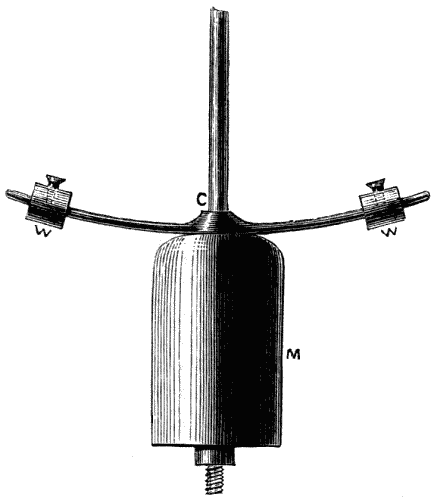
\includegraphics[width=0.8\textwidth]{images/fig10.png}
\label{fig10}
\end{figure}
and old Mr.~Dent told me it was found inferior to the other
methods, over which I do not see that it has any advantage
except the facility of adjustment. It is said in Kater's
treatise to have answered in France, but the French seem to
prefer complicated compensations to simple ones. It might
however be used to complete the adjustment of another
compensation left imperfect for that purpose, in which case
the weights would only need to be very small.
%-----File: 079.png--------------------------------------------
%-----Folio: 64------------------------------------------------

\subsection[Homogeneous compensation.]{Homogeneous compensation.}\markboth{HOMOGENEOUS COMPENSATION.}{HOMOGENEOUS COMPENSATION.}\label{subsec:Homogeneous_compensation.}\index{Compensation of pendulums!homogeneous}\index{Homogeneous compensation}\index{Pendulums!compensation!homogeneous}---All the compensations
I have yet mentioned require the use of at least two substances
of different expansibility;   but there is one which
does not; and though it is practically of little or no value,
in any form in which it has yet been made or suggested, it
is worth while to describe the principle of it. If the
pendulum spring is drawn up through a close slit in the
cock as much as the pendulum lengthens by heat, its
effective length will remain the same; and this may be done
by various arrangements, of which the simplest is hanging
the spring to another cock above the slit one, set on the top
of a stiff bar long enough to expand upwards as much as the
pendulum rod expands downwards. This bar may be either
of the same or of a different metal from the pendulum rod
and its length will of course depend
on its material; or the slit
cock may be on one end of a lever,
of which the other is pulled down
by a wire of the same length and
metal as the pendulum rod. But
there is a serious objection to this
plan in every form; if the slit is
loose enough to let the spring slide
up and down through it, it is too
loose for the proper action of the
pendulum in a clock good enough
to require a compensation for temperature.
There is no other kind
practically worth describing.

\begin{figure}[htbp]
\centering
\hypertarget{fig11}{\caption{\sc Ellicott's Compensation Pendulum}}
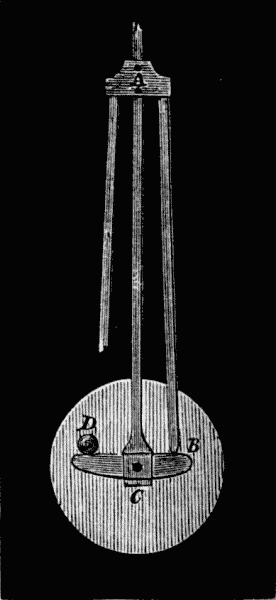
\includegraphics[width=0.5\textwidth]{images/fig11.png}
\label{fig11}
\end{figure}
\subsection[Ellicott's pendulum.]{Ellicott's pendulum.}\markboth{ELLICOTT'S COMPENSATION PENDULUM.}{ELLICOTT'S COMPENSATION PENDULUM.}\label{subsec:Ellicott's_pendulum.}\index{Compensation of pendulums!Ellicott's}\index{Ellicott's compensation pendulum}---There
is another bad one which is still
used in small French clocks,
though it has long ago been abandoned
in England, where it was
invented by Ellicott a clockmaker
%-----File: 080.png--------------------------------------------
%-----Folio: 65------------------------------------------------
in the last century. $\mathrm{AC}$ the main rod is of iron or
steel and it has a pair of levers set on a cross pin at
the bottom, of which only one $\mathrm{BCD}$ is shown \hyperlink{fig11}{here}: at
$\mathrm{A}$ there is a strong collar fixed to the rod, and between
that collar and the short arm of each lever stands a stiff
brass rod. The bob hangs by two pins, of which $\mathrm{D}$ is one,
on the long arms of the levers; and it is evident that by a
proper adjustment of the levers the bob may be made to
rise under the expansion of the brass rods just as much as
the expansion of the iron rod lets down $\mathrm{C}$, the axis of the
levers. But this action involves considerable friction at $\mathrm{D}$,
and the pressure on the ends of the brass rods must very
much exceed the weight of the pendulum, and it is said to
move by jerks, and is altogether inferior even to the old
gridiron, and much more to the zinc or mercurial pendulum,
besides being much more difficult to make properly. I
suppose they are only made because they have a kind of
scientific look to ignorant people, in clocks made to show
and to sell.

\subsection[Mercurial compensation.]{Mercurial compensation.}\markboth{MERCURIAL COMPENSATION.}{MERCURIAL COMPENSATION.}\label{subsec:Mercurial_compensation.}\index{Compensation of pendulums!mercurial}\index{Mercurial compensation}\index{Pendulums!compensation!mercurial}---The principle of this, which
is used in all the best astronomical clocks (subject to a
remark to be made afterwards), is the same as of the wood
and lead; only, mercury being fluid requires a different mode
of calculation. For it must be in a jar which has some
sideway expansion of its own, and the rise of the mercury is
only the excess of its expansion in bulk over that which the
increased width of the jar allows it. The jars can only be
made of either glass or iron, as mercury amalgamates with
and so destroys any other metal that could be used. Although
iron is the best, glass is the most commonly used, either
from old habit or ignorance, and so we must consider both
of them, and we will take the glass first, and in both cases
neglect at first the weight of the jar itself: which by a
strange oversight was forgotten altogether by Francis Baily,
P.R.A.S., in a far more elaborate paper on this subject
%-----File: 081.png--------------------------------------------
%-----Folio: 66------------------------------------------------
(in vol.~i.\ of their Memoirs) than there is any need of, seeing
that after all a compensated pendulum can only be accurately
adjusted by trial, of itself or one exactly like it. It is
almost equally strange that this mistake was never discovered
for forty-four years, though the best clockmakers
and the late Mr.~Bloxam\index{Bloxam!his escapements}\index{Bloxam!corrected Sir G.~Airy}, who most thoroughly investigated
the theory of escapements in two papers in the 22nd and
27th vols.\ of the R.A.S.\ \textit{Memoirs}, had practically found that
the received height of mercury was insufficient. But they
all attributed it to the pendulum spring being stiffer in cold
than heat; which always appeared to me a most inadequate
explanation, considering the weakness of the spring in
proportion to the weight of a pendulum. In 1863 I had
to calculate the height for the iron jar of a pendulum
intended to weigh $40$~lbs., and finding the result far
beyond Baily's proportions, I looked carefully through his
paper and then found out the mistake\index{Baily, F.!his mistake on pendulum compensation}\index{Compensation of pendulums!Baily's mistake on}\markboth{BAILY'S MISTAKE ABOUT MERCURIAL COMPENSATION.}{BAILY'S MISTAKE ABOUT MERCURIAL COMPENSATION.}, and published the
correction of it in the \textit{Mechanics' Magazine}, of 5~Feb.~1864.
Another reason why it had escaped discovery was that dead
escapements, which nearly all astronomical clocks had,
contain (as I said before) an irregular kind of compensation
of their own, from the greater fluidity of the oil in warm
weather. It is remarkable that Hardy, the inventor of
another kind of escapement which I shall notice afterwards,
had calculated the height of his mercury rightly before
Baily's paper which everybody accepted.

\begin{wrapfigure}{o}{146pt}
\centering
\hypertarget{fig12}{\caption{\sc A new kind of jar}}
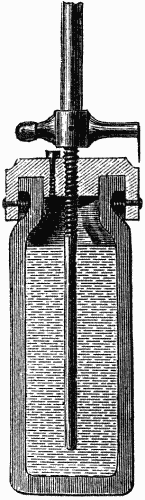
\includegraphics[height=500pt]{images/fig12.png}
\label{fig12}
\end{wrapfigure}
Mercury expands $.1$ in bulk while the glass jar increases
$.0048$ in diameter, and $\therefore$ the sectional area increases as
$(1.0048)^2$ or $1.0096$ to $1$; $\therefore$ the mercury will rise $.1$--$.01$
(say) or $.09$ of its own height. And since the c.g.\ of the
bob is very nearly at $\mathrm{O}$, let $x$ be half the height of mercury;
then $.09x$ must be $=.0066(l+x)$ for the steel rod, which is
usually carried down to the bottom of the jar in the form of
a long `stirrup,' on which the jar stands. That makes $x=3.1$~in.\ or
the height of the mercury $6.2$~in., which has to
%-----File: 082.png--------------------------------------------
%-----Folio: 67------------------------------------------------
be increased $.1$, or rather more for a reason which will
appear afterwards, and that is Baily's result---without
considering the weight of the jar.

The weight of the glass jar and rod may be a $6$th of
the ultimate or corrected weight of the mercury; and about
much more height must be added for it, as it is evidently
much the same as if all the bob of pendulum were mercury,
but its rise only $\frac56$ of its real amount. And approximately
this is near enough, seeing that pendulums vary in their
proportions and must be finally adjusted
by trial; and glass jars are going out
of use for the best pendulums, which it
is now agreed ought to be much
heavier than the old two-inch wide
cylinder allows.

The late Captain Kater\index{Kater!his mercurial pendulum}\index{Mercurial compensation!Kater's and Beckett's} used for
his experiments entirely glass pendulums,
which of course require a less
height of mercury than steel ones.
There is however no advantage in that,
but rather the contrary, as the jar must
be inconveniently wide to hold any considerable
weight, besides the difficulty
of handling a heavy glass pendulum
safely. Others have made the steel rod
go through the bottom of the jar; but
that is a bad plan, as it involves
stuffing to make the hole mercury-tight,
and allows no subsequent adjustment
without risk of destroying that
tightness. It is desirable however that
the rod should plunge into the mercury,
that they may take the same temperature, and
the best way of doing this with a glass jar would be
that shown in \hyperlink{fig12}{this drawing}. The shape of the jar speaks
%-----File: 083.png--------------------------------------------
%-----Folio: 68------------------------------------------------
for itself. The black ring round the neck is in two
pieces  of brass, put on with a piece of thin leather to
improve the fitting, before the cap is dropped over it and
screwed to them with two or three screws to each half of the
ring. All other plans with the same object that I have seen
involved some cementing to the glass or stuffing, which is
not to be trusted. The small hole in the cap is for adjusting
the quantity of mercury according to experience.

\subsection[Cast iron jars]{Cast iron jars}\markboth{CAST IRON JARS.}{CAST IRON JARS.}\ \label{subsec:Cast_iron_jars}are superior\index{Cast iron jars best for mercurial pendulums}\index{Mercurial compensation!Cast-iron jars for} to glass, first because they
are safer, and firmer on the rod, and the construction
simpler when done properly; secondly, because the mercury
can be heated in them to drive off any moisture or air
bubbles between the mercury and the jar, as is done with
barometers; thirdly, because (contrary to the common
notion) the extra height required for the weight of the jar is
an advantage, especially when you want a very heavy bob.
Calling the jar about a third of the mercury in weight, a
$40$~lbs.\ pendulum will have a jar only $3\frac12$~in.\ wide outside;
and one \textit{holding} $40$~lbs.\ of mercury will be $3\frac12$~in.\ inside, for
we shall find the mercury to be nearly $9$~in.\ high, and a
cubic in.\ of pure mercury weighs half a pound, and common
mercury weighs slightly less. The best construction,
and much cheaper than that generally used till lately, is
to cast the jar $\frac14$~in.\ thick, and twice as long as it need
be, in order to secure sound casting, as they do for cannon,
cutting off the `dead head;' turn the outside if you like
for appearance, or else japan it, and `enamel' the inside,
\textit{i.e.\ }coat it with glass, which stops up all the pores. The
cap is partially dropped into the top of the jar just turned
out to fit it and held by $4$ or $5$ screws through the jar. The
rim is marked out into divisions of $1$~sec.\ a day as described
at p.~\pageref{marks}, an index being fixed to the steel rod, which is
tapped and screwed through the cap exactly as in the last
figure, while the cross-head is to hold it steady when you
turn the jar for regulating. A $40$~lbs.\ pendulum made thus
%-----File: 084.png--------------------------------------------
%-----Folio: 69------------------------------------------------
costs less than old Mr.~Dent used to pay for the pendulum
alone without the mercury, on the old construction. This
is the construction now used by Mr.~Brock of 64, George
Street, Portman Square, who used to be with Dent, and has
done all except church clock work for me for some years.
Enamelling the jars was his idea.

For an approximate calculation like the last, we have only
to use the expansion $.0066$ of cast iron instead of glass for
the jar, and that makes the rise of the mercury $.1-.0132$ or
$.087$ nearly. And assuming the mercury to weigh $3$ times
the jar and rod, the rise must be $\frac43$ times as much as if they
had no weight, or we may treat the rise of the mercury
relatively as $.065$, or $\frac34$ of its real amount. We know that
the height must be something over $8$~in., and the total length
of the pendulum nearly $43\frac12$, allowing the c.g.\ of the bob
to be a very little above $\mathrm{O}$\@. It is not worth while to
distinguish between the expansion of cast iron and steel for
the short length of the cylinder, and we may say that the
rise of the c.g.\ of the mercury, or the increase of $x$, or
$.065x$, must $=43.5\times.0064 =.2784$, and $\therefore x= 4.3$
nearly. The assumption that $x$ is something over $4$~in.,
for the mere purpose of finding the total length of the rod,
does not affect the result sensibly, as you will see if you try
it as an inch more or less. But this is not quite enough,
because it is not the c.g.\ but the c.o.\ that has to be kept at
the same height, and we must find how much less $h$ really is
than $l$ for we have only yet stated it approximately. If $b$
is the radius of the cylinder when the weight of the rod is
insignificant, $lh=k^2$ or $ = k^2+\frac{x^2}{3}+\frac{l^2}{4}$.\ but $b$ is so small
compared with $h$ that that term produces no sensible effect.
Then putting $39.14$ for $l$ and either $4.3$ or $4.4$ for $x$ you
will find by solving the quadratic equation that $h=38.98$
or $l-h=.16$~in.\ = $.036x$: $\therefore$ we must say $.964\times.065x$
or $.0626x=.2784$ as before, and $\therefore x=4.44$, which
%-----File: 085.png----------------------------------------------
%-----Folio: 70--------------------------------------------------
makes the height of mercury just under $9$~in.\ in a jar which
weighs $\frac13$ of the mercury. I found mine not quite enough
compensated with $8\frac12$~in., and it is perhaps a little over
done with $9$---a widely different result from Baily's $6.6$ for
an iron jar. The calculation of compensation otherwise
than by this method of approximation runs into equations
of a high order and becomes unmanageable, and after all it
is better to adjust the height of the mercury finally by trial.
The longer the bob is, or the heavier the rod and compensation
tubes, the more the c.g.\ of the bob (not of the whole
pendulum) is below c.o. A very long bob is not desirable
on account of the increased resistance of the air\index{Air!resistance of to pendulum}, and
therefore it is not expedient to make the jar more than
about a third of the weight of the mercury, which is in every
way a convenient size.

\markboth{MERCURIAL V.\ ZINC COMPENSATIONS.}{MERCURIAL V.\ ZINC COMPENSATIONS.}It is now thought at Greenwich that zinc and steel\index{Zinc!zinc and steel pendulums!better than mercurial} pendulums
are as good as mercurial ones. The normal sidereal
clock there has a zinc pendulum, and I am told that its daily
variation of rate is reckoned by hundredths of a second.
If this is so, it will be a considerable saving in expense,
inasmuch as there is no doubt that pendulums ought to be
much heavier than used to be the fashion. I must say that
the performance of the great Westminster clock goes far
to confirm the Greenwich opinion, for it has no discoverable
error of temperature.

\subsection[Barometric compensation.]{Barometric compensation.}\markboth{BAROMETRIC ERROR OF CLOCKS.}{BAROMETRIC ERROR OF CLOCKS.}\label{subsec:Barometric_compensation.}\index{Barometric compensation}\index{Compensation of pendulums!barometric}\index{Mercurial compensation!Barometric}---It is evident that the
larger the bob is for its weight, \textit{i.e.\ }the less its specific
gravity, the more it will be resisted by the air, and the
smaller arc it will swing under a given force. We shall see
afterwards that all the escapement errors involve $\frac{\mathrm{W}h}{\mathrm{M}l}$
divided by either $a^2$ or $a^3$, $\mathrm{W}h$ being the force that actually
drives the pendulum for a day, or weight $\times$ daily fall, after
deducting the friction, and $\mathrm{M}l$ the same as before, and
the arc from zero as usual. Therefore the larger $a$ is
%-----File: 086.png-----------------------------------------------
%-----Folio: 71---------------------------------------------------
\textit{for a given weight} the better a great deal. Moreover, the
greater the density of the air\index{Air!barometric effect of} is, the more it diminishes
the effective specific gravity of the pendulum, viz., by
an amount $=$ sp.~g.\ of the air, which is variously estimated
at something near the $840$th of that of water, and therefore
about a $9000$th of an ordinary lead pendulum with
deal rod, or a mercurial one with a glass jar and the usual
appendages, which make its mean sp.~g.\ about $11$, water
being $1$. And this reduction is considerably increased in a
swinging pendulum by the air which it drags along with it.
Baily\index{Baily, F.!on barometric compensation} found, by comparing the times of free pendulums
of various kinds in vacuo and in air (see \textit{Phil.~Trans.}~of
1832), that the stationary loss of sp.~g.\ is sometimes
doubled by vibration. One specially curious result should
be noted, that a thin flat rod with a very elliptical section
was more affected in this way than a round one three times
as thick, although a lens-shaped bob was less affected than
a sphere of the same diameter and of course much heavier in
proportion to its surface, which so far gives it an advantage.
But we have no information whether the air affects a lens
more or less than a sphere of the same weight.

Bloxam\index{Bloxam!on barometric error}\label{barerr} said in a note to his paper in the R.A.S.\ \textit{Memoirs}
of 1853 that Baily overlooked the fact that the current
produced in the descent of the pendulum prevents it from
being retarded in the ascent as much as it would have
been if the air had been at rest. He also always found the
circular error to be less than its theoretical value, and the
resistance of the air doubtless tends to produce this effect.

Without going through Baily's various results it is enough
to say that he found pendulums of sp.~g.\ about $11$ gain
nearly $13$~sec.\ a day by being put into a vacuum; as that
was the daily increase of time ($+ \Delta\mathrm{T}$ or $-$ `rate') for an
inch rise of barometer, which is shortly called the barometric
error, apart from any circular or escapement error which
may accompany it. A small platinum ball hung by a wire
%-----File: 087.png-----------------------------------------------
%-----Folio: 72---------------------------------------------------
gained $5$~sec.\ in vacuo, against $9\frac12$ for a lead one of the
same size (for a sphere is less affected than a cylinder); the
gain was nearly $14$ for a brass and $56$ for an ivory ball, and
$19$ for a round copper rod $.41$~in.\ thick and $5$~ft.\ long;
which last was $3$ times as much as its stationary loss of
specific gravity. But this effect on the rod as a whole
pendulum is insignificant when it carries a bob much heavier
than itself, as it usually does.

\index{Large and small arcs}Baily\index{Baily, F.!on barometric compensation} found also by calculation that with an arc of $2^\circ\ 45'$
the barometric error ought to be neutralized by the circular
error, \textit{i.e.\ }by the diminution of arc\index{Arcs of vibration in clocks} produced by the
increased density of the air. That result differs from the
one arrived at by Bloxam, but was verified by the performance
of the Westminster\index{Westminster clock!has no barometric error} clock during the year 1872, in
which I ascertained that the barometric error does not exist\label{fully},
\textit{i.e.\ }is exactly neutralized, by the fact that applying any
correction, either $+$ or $-$, bearing a constant proportion to
the actual variations of the barometer, would have increased
the small average variation of the clock. I mention as a
fact, without professing to account for it, that Bloxam found
the barometric error of his clock \markboth{VALUE OF LARGE ARCS.}{VALUE OF LARGE ARCS.}less with an arc of $90^\circ$ than
with a considerably larger one. But I am decidedly in favour
of large arcs, especially for large clocks exposed to greater
variations of force than small ones, and I adopted one at
Westminster before I knew that it agreed with Baily's
calculation, which it has so remarkably verified.

In order to avoid the barometric error,\markboth{BAROMETRIC COMPENSATION.}{BAROMETRIC COMPENSATION.} Mr.~Carrington
adopted the plan of a perfectly air-tight clock case\index{Air-tight clock-case}\label{airtight}, the
winder going through a `stuffing-box,' and then he
exhausts the air down to some given pressure a few inches
below the usual height of the barometer (see R.A.S.\ \textit{Notices}
of Nov.~1872). But this is much too troublesome for common
use. Dr.~Robinson\index{Robinson, Dr., on barometric compensation of pendulums}, of the Armagh Observatory, long ago
adopted the much simpler plan of compensating the error by
attaching a pair of very thin barometers on the right and
%-----File: 088.png-----------------------------------------------
%-----Folio: 73---------------------------------------------------
\label{therm}left sides of the pendulum rod, above the bob (R.A.S.\ \textit{memoirs}
vol.~5). This evidently has the effect of raising a
small weight of mercury from near the bottom of the
pendulum to near the top when the density of the air
increases, and \textit{vice vers\^a}. But I shall presently point out
an inconvenience of this mode of doing it, and Dr.~Robinson
expressly says that the adjustments were troublesome.
The barometric error also varies considerably even between
clocks of nominally the same kind; so much that it is not
safe to assume any given amount beforehand, but it must be
ascertained from observation of that particular clock before
the calculations are made for correcting it. In the best
kind of astronomical clocks, with detached, or with gravity
escapements, but not dead ones, we may take the daily loss
($+\Delta\mathrm{T}$) for the present at $0.3$~sec.\ a day for an inch rise
of barometer, or that is the barometric error so far as it is
unconnected by others which attend it.

In a paper on this subject in the R.A.S. \textit{Monthly Notices}
of 1873 I remarked that two barometers are unnecessary,
because a slight want of symmetry in (not across) the plane
of vibration cannot affect the pendulum. Moreover, with a
bob of the length required for an iron jar mercurial pendulum
there is not room to put the barometer tube entirely
above the jar. What we have to do is to find the position
and the diameter $2x$ of the barometer which fixed at some
given height will thus compensate a $39$~inch pendulum of
given weight, say $40$~lbs. It is tempting at first sight to
make the great mercury jar serve as a basin for the
barometer; but there are various practical objections to it,
and it is much better to use a syphon tube bent over the
side of the jar, in which therefore a `rise of barometer' of
$r$~in.\ will be only an absolute rise $r$ of $\frac12$~in.\ in the longer
leg, with a fall of $\frac12$~in.\ in the shorter. Let the mercury in
the long leg reach to $d$ below the top of the pendulum, and
in the short one to $b$ above the centre of oscillation: $\rho$, the
%-----File: 089.png-----------------------------------------------
%-----Folio: 74---------------------------------------------------
specific gravity of mercury, is such that a cubic inch of
mercury is very nearly half a pound. Then, by the same
mode of calculation as at p.~\pageref{p50calc}, the little weight transferred
from $b$ to $d$ being $\pi\rho x^2 r$,
\[
-\Delta\mathrm{T} = \frac{43200\pi\rho x^2r}{\mathrm{M}}
\frac{ld-d^2+b^2-lb}{l^2} \mbox{ sec.},
\]
or putting $\frac14$ for $\rho r$ and $40$ for $\mathrm{M}$ we must have (nearly)
\[
850 x^2 \frac{ld-d^2+b^2-lb}{l^2} = .3.
\]
Now $d$ must be substantially $> b$ for this to keep its sign,
and also to keep tolerably constant for different degrees of
rise. For simplicity let $b = 0$, and $\therefore d = 9$~in.: this gives
$2x$ or the diameter of the tube $.03$~in. If the barometric
error is $3$ times as much, $2x$ must be $\surd{3}$ times as much or
about $.05$; in either case rather a thermometer tube than a
barometer one. The tube, after being bent over and down
either the right or left side of the jar, had better be brought
up to the rod again, and the two branches joined there by
heat for strength, and tied to the rod by waxed thread rather
than any metal fastening. If the compensation is found to
be overdone the tube has only to be untied and raised, and
if insufficient it may be lowered, if room enough has been
left for it in the bend.

As the barometric error never lasts long in one direction
it will very seldom be thought necessary to apply the compensation
to large clocks; and we have seen that it can be
otherwise materially reduced, if not absolutely corrected, as it
is in the Westminster pendulum, by making it swing a large
arc. If it were necessary to apply the barometric compensation
to a long pendulum the best way would be to put an
annular basin for the mercury on the top of the bob, round
the compensation tubes, and have a straight barometer
dipping into it. It may easily be calculated that the same
barometric error of $.3$~sec.\ a day with a $1\frac14$~sec.\ pendulum of
$200$~lbs., and also with a $1\frac12$~sec.\ pendulum of $300$~lbs.
%-----File: 090.png-----------------------------------------------
%-----Folio: 75---------------------------------------------------
would be corrected by a barometer tube of about a sixth of
an inch diameter. The reason why the same tube is
enough for the heavier pendulum is that the rise of the
mercury is in a more effective place, \textit{i.e.\ }near the middle of
the pendulum. A $13$~ft.\ pendulum of $700$~lbs.\ with the
lower surface of the mercury $6$~in.\ above c.o.\ requires a
tube of $.3$ diameter for the barometric error of $.3$ sec:
another odd coincidence of figures. If the barometric error
in any particular clock is found to be $2$ or $3$ times as much
as this, $2x$ or the diameter of the tube must be $\surd{2}$ or $\surd{3}$
as much as the above figures, and it must vary in the same
way with the $\sqrt{\textrm{weight}}$ of the pendulum. We shall have to
consider this further when we come to escapements.\index{Escapements of clocks}

The normal sidereal clock at Greenwich\markboth{GREENWICH BAROMETRIC COMPENSATION.}{GREENWICH BAROMETRIC COMPENSATION.} has a barometric
compensation\index{Greenwich!barometric pendulum compensation at}\label{grenplan} of a more complicated kind. An independent
fixed barometer raises and lowers a \index{Magnet used for regulating clocks}magnet which attracts
the pendulum more or less according to its position. I must
say that seems to me a roundabout way of doing the
business, and I should have been inclined first to try a large
arc of $2^\circ\ 45'$ like that of the Westminster clock, and if that
is not sufficient, then the simple barometric tube compensation,
with the bottom of the tube near the bottom of the
bob.

\section{RECOIL ANCHOR PALLETS.}\label{sec:RECOIL_ANCHOR_PALLETS.}\index{Anchor pallets}\index{Pallets!anchor}\index{Recoil!anchor pallets}\markboth{ANCHOR PALLETS.}{ANCHOR PALLETS.}

The next important invention which followed that of
pendulums, and that very soon, was a pair of anchor-like
pallets moving in the plane of the scapewheel, instead of the
`vertical escapement' with pallets set across a crown wheel,
which pallets being very short required a long swing of
the pendulum to let the wheel escape. It is not indeed
absolutely necessary that crown wheel pallets should be
very short, and they would go with less friction if they were
long and the teeth of the wheel few; but the recoil would
be more violent, and they would require more careful adjustment,
%-----File: 091.png---------------------------------------------
%-----Folio: 76-------------------------------------------------
and as a matter of fact they always were short.
Anchor pallets in the form in which they were first invented
either by Dr.~Hooke\index{Hooke, inventor of the balance-spring of watches}, whom I have already mentioned as
one of the claimants of the pendulum, or by Clements, a
London clockmaker of his time, had a recoil, no less than
the crown wheel pallets, but they could be made to escape at
as small an arc as you please. Fig.~\ref{fig13} is a drawing of the
recoil escapement, as it is always called, which is still used
in all the common
clocks in the world,
though it has long
been abandoned in all
that make any pretension
to great accuracy.

\begin{figure}[hbtp]
\centering
\hypertarget{fig13}{\caption{\sc Anchor Pallets}}
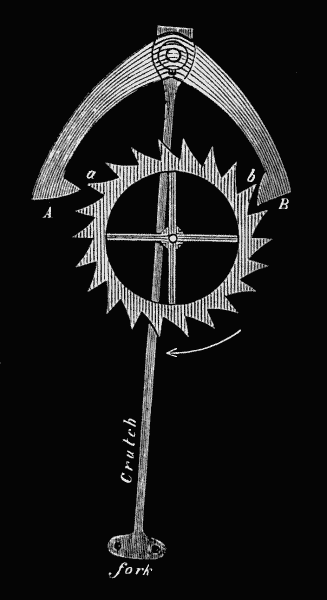
\includegraphics[width=0.7\textwidth]{images/fig13.png}
\label{fig13}
\end{figure}

In \hyperlink{fig13}{this figure} the
tooth $a$ has just escaped
from the left
pallet $\mathrm{A}$, and $b$ has
dropped on to pallet
$\mathrm{B}$; the pendulum is
therefore moving to
the left, and it will
not stop immediately
but will go on a little
farther and so make
the wheel recoil a
little, as you may see
clearly enough in any
old-fashioned house
clock with a seconds
hand: as it returns,
the wheel urges the
pendulum again to the
right and so gives the
%-----File: 092.png---------------------------------------------
%-----Folio: 77-------------------------------------------------
\index{Escapements of clocks!recoil}\index{Recoil!escapements}%
impulse which is necessary to maintain its motion against
the resistance of the air and the friction of the escapement
itself; and then tooth $b$ escapes, and the tooth below $a$ falls
on $\mathrm{A}$ and the same action takes place there. You observe
that I have drawn the acting faces convex. For
some theoretical reasons they ought to be concave; but,
as very often happens in clockwork, the one practical reason
of friction preponderates the other way. Even if they are
made flat, the teeth always wear holes in them, though the
teeth are of brass and the pallets of steel, made as hard as
possible, and it is evident that the friction at the recoil is
much greater if the pallets are concave than convex. Moreover
it is always found that as the pendulum arc decreases
from any decrease of force in the clock, it loses and \textit{vice
vers\^a;} and concave pallets would not diminish this error,
but increase it. Some considerable persons stuck to this
escapement for some time after the dead escapement was
invented, being apparently misled by the fact that variations
of force produce less variation of the \textit{arc} in this than in the
dead escapement, because the friction of the recoil checks
the arc; but it does not follow that the variations of \textit{time}
are less: in fact it has been proved both by experience and
calculation that they are not.

I may as well mention here that a `steady rate' means,
not necessarily that the clock is going \textit{right}, but that it is
going \textit{uniformly}, or regularly gaining or losing exactly the
same number of seconds a day or a week. The rate is
always written $+$ when the clock gains, and $-$ when it
loses; which you must remember is just the opposite of the
signs appended to the expressions for the various errors of
the time in the mathematical formulae; for when $t$ the time
of vibration of the pendulum increases, $dt$ is $+$, and the
clock loses and the \textit{rate} is too little or $-$.

\subsection[Harrison's recoil escapement]{Harrison's recoil escapement}\markboth{A POSSIBLE RECOIL ESCAPEMENT.}{RECOIL ESCAPEMENTS.}\ \label{subsec:Harrison's_recoil_escapement}\index{Recoil!escapements!Harrison's}\index{Harrison!his clock escapement}had scarcely any friction.
It was invented by him when he was a working
%-----File: 093.png---------------------------------------------
%-----Folio: 78-------------------------------------------------
carpenter in Lincolnshire. Any one who  wants to see a
description of it will find one in the 7th edition of the
\textit{Encyclop\ae dia  Britannica}; but I did not think it worth
while to repeat it in the 8th; nor here, as it is a mere
obsolete curiosity, and nobody else ever made it to answer,
even before better things were invented. If such a thing
were worth doing, it might be done much more simply by a
three-legged scapewheel, such as I  shall describe as one
form of the dead escapement (at p.~\pageref{subsec:Three-legged_dead_escapement.}), but without the
horizontal or dead pallets there, and with the impulse pallets
set deeper and not in the same line, though parallel to the
pendulum. The impulse would be given with nearly as
little friction\index{Friction rollers!for clock barrel} as it is there, and the recoil would also have
very little; and if the force on the scapewheel were made
uniform, as it may be by a contrivance which I shall describe
for turret clocks, there is no reason why such an
escapement should not go very well, though the dead one
would go better.

\subsection[Clock out of beat.]{Clock out of beat.}\markboth{CLOCKS OUT OF BEAT.}{CLOCKS OUT OF BEAT.}\label{subsec:Clock_out_of_beat.}\index{Clock out of beat, to regulate}---Most people seem to know that
the beats of a clock ought to sound equal in time, but most
people have a very erroneous notion that this depends on the
clock being set on a perfectly level surface, or standing vertically;
whereas that has nothing at all to do with it, unless
the crutch has been so adjusted that the pallets do escape at
equal angles when the clock case stands upright. No doubt
they ought to be so adjusted\index{Beat!adjustment of}, because a clock looks better
standing straight than crooked. In the best clocks the
beat is made adjustable by beat-screws at the bottom of the
crutch or fork. In common ones it is simply bent by hand
till the beats sound equal. Mr.~Dent made the fork pins
in turret-clock escapements to open with a spring, to prevent
the teeth being damaged in case they should be caught by the
escaping corner of the pallets when the clock is put back, or
the pendulum set going without the clock being wound up.
Each `prong' of the fork must have a separate spring, both
%-----File: 094.png--------------------------------------------
%-----Folio: 79------------------------------------------------
set against a stop between them. The crutch and everything
attached to the pallets ought to be kept as light as
possible,  because they are in fact a pendulum, moving on
pivots instead of a spring, and therefore with much more
friction than the real pendulum. But a long crutch is
better than a short one, because less angular motion and
force is lost in the looseness or `shake,' which, as I explained
at p.~\pageref{shake}, must be left between the fork and the
pendulum. The proper way to try whether a clock is in
beat is to let the pendulum swing only just far enough
for the escape, and then you will easily hear if the beats are
unequal.

When a clock with any kind of anchor escapement (which
all clocks may be assumed to have, unless the contrary is
known) sounds `out of beat,' it wants either one side lifting
or the crutch bending---which you please. If the right-hand
beat of the pendulum (\textit{i.e.\ }the blow on the left-hand pallet)
comes too quick, the right pallet escapes too soon or does
not go deep enough. Therefore the right side of the clock
wants lifting; for that is equivalent to moving the pendulum
and pallets to the left. Or it wants the fork or bottom of the
crutch bending to the right, which, remember, is making a
bend \textit{in} the crutch to the left, for that carries the pallets to
the left. Or if there is a beat screw in the fork, it wants
turning to the right or `setting up,' so as to move the
crutch to the left. And \textit{vice vers\^a}, if the left beat comes
too quick, the left side of the clock wants raising, or
the fork tending to the left, or the beat screw turning to
the left.

I shall notice afterwards, under French clocks, a contrivance
which some of them have to make the beats gradually
adjust themselves. Recoil pallets---and dead ones too---should
only just clear the teeth, and when the points get
worn so as to allow more clearance the pallets should be
renewed.
%-----File: 095.png--------------------------------------------
%-----Folio: 80------------------------------------------------




\section{DEAD ESCAPEMENTS.}\label{sec:DEAD_ESCAPEMENTS.}\index{Dead escapements}\index{Escapements of clocks!dead}\markboth{THEORY OF THE COMMON DEAD ESCAPEMENT.}{THEORY OF THE COMMON DEAD ESCAPEMENT.}

\begin{figure}[tbp]
\centering
\hypertarget{fig14}{\caption{\sc Dead Escapements}}
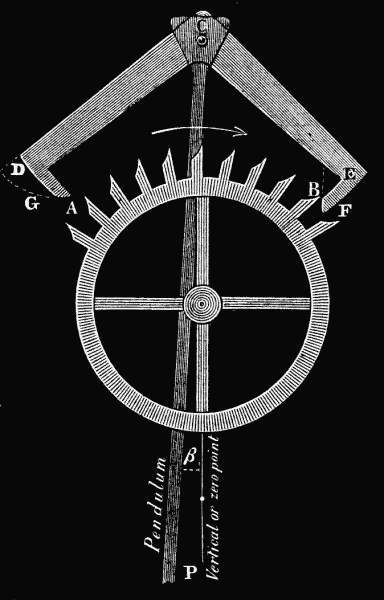
\includegraphics[height=0.7\textheight]{images/fig14.png}
\label{fig14}
\end{figure}
These are also of the anchor kind; but in fig.~\ref{fig14}, as in
fig.~\ref{fig13}, a tooth of the scapewheel has just escaped from
pallet $\mathrm{A}$ and another has just fallen on to pallet $\mathrm{B}$; but the
face on which it falls is very different, as the shape of the
teeth also is, but
that is only to
give room for
clearance, and in
both cases it is
only the point of
the tooth that
acts. \hyperlink{fig14}{Here}, you
see the face of the
pallet is divided
into two, and one
part is an arc of
a circle of radius
$\mathrm{CB}$ while the
other part is
much the same
as it was in the
recoil pallets.
The consequence
evidently is that
there is no recoil
here, and the
tooth lies \textit{dead} on
the circular face
$\mathrm{BE}$ (which is
therefore called the dead face) however far the pendulum may
swing, until it returns to $\mathrm{B}$, and then the tooth begins to act
on the impulse face and gives the impulse to the pendulum
exactly as in the other escapement.    In the same way the
%-----File: 096.png---------------------------------------------
%-----Folio: 81-------------------------------------------------
dead face $\mathrm{DG}$ of the other pallet is part of a circle with
radius $\mathrm{CD}$: the dotted line being the old recoil shape.

This is the dead escapement, which was invented early in
the last century by Graham\index{Dead escapements!Graham's}\index{Graham's!dead escapement}\label{dead}, who invented also the mercurial
pendulum and the horizontal watch escapement; and
the great advantage of it is that although a slight increase
of force on the scapewheel increases the arc of the pendulum,
it does not sensibly increase the time, if the escapement is
properly made. This was first demonstrated mathematically
by Sir G.~Airy\index{Airy, Sir G.~B.!his calculations for dead escapements}, in the \textit{Cambridge Philosophical Transactions}
in 1827 (Vol.~III.\ p.~105), and it may be made tolerably
clear without any mathematics, as follows. If each tooth
could drop exactly on the corner dividing the dead and impulse
faces of the pallet, as at $\mathrm{B}$, it is clear that the impulse
on each pallet would begin and end when the pendulum is at
the same distance on each side of zero or the vertical. In other
words, as much of the impulse would be given while the pendulum
is falling as while it is rising, and therefore its gravity
would be increased on one side and diminished on the other
through equal arcs and during equal times, and therefore on the
whole the accelerating force on the pendulum, and therefore
its time of vibration, not altered. Neither would the friction
on the dead faces, if it were constant throughout, and if it
acted through the same arcs before and after zero, affect the
time directly; for while the pendulum is falling the friction
acts contrary to gravity, and with gravity while it is rising
after the escape has taken place. As it is always resisting
the motion of the pendulum it tends to diminish the arc;
and on the other hand, the impulse always tends to increase
it; so that here also there is counteraction to some extent;
but as the friction on the pallets does not vary in any
definite proportion to the force of the train, but sometimes
one way and sometimes the other, no useful relation of this
kind can be established. All we can say about the arc is
that it increases under an increased force or a diminished
%-----File: 097.png--------------------------------------------
%-----Folio: 82------------------------------------------------
friction, until the remaining friction on the pallets and the
resistance of the air stops the increase.

Mr.~Bloxam\index{Bloxam!his escapements} came to the conclusion, in his elaborate
papers on escapements in vols.~22 and 27 of the \textit{Astronomical
Society's Memoirs}, that so far from the dead friction\index{Dead escapements!effects of friction on}\label{friction}\index{Friction!in dead escapements}
being a thing to be disregarded as constant and not
materially affecting the rate of the clock, as Mr.~Airy\index{Airy, Sir G.~B.!his calculations for dead escapements} had
assumed, it probably affects it more than all the other escapement
errors together in an astronomical clock\index{Astronomical clocks}\index{Clocks!astronomical} with even a
moderately good train, and in a way which it is impossible
to calculate on account of the different circumstances under
which it varies. It is evidently very improbable that the
friction can be made the same while the point of the tooth is
(as we may say) ploughing its way up the pallet during the
ascent of the pendulum and sliding down it in the descent.
Having said this I shall not attempt to deal any farther with
the dead friction, but its existence must be borne in mind as
capable of either mitigating or increasing the other errors,
as the case may be; and some idea of the magnitude of its
effects may be formed from this, that I remember the arc of
a new church clock of Mr.~Vulliamy's increasing from
$2^\circ 30^\prime$ to $30^\circ 30^\prime$ in the first year, from no other visible cause
than the self-polishing of pallets. And it afterwards fell off
again from the pins of the heavy scapewheel wearing hollows
in the pallets where they dropped.

Now\markboth{THEORY OF DEAD ESCAPEMENTS.}{THEORY OF DEAD ESCAPEMENTS.} let us apply the same reasoning to the recoil escapement,
and we shall find that the result is just the opposite
from that in the dead. That part of the impulse which is
within the points where the teeth fall on the pallets is the
same as in the dead escapement, and therefore may be taken
not to affect the time; but in the ascending portion of the
recoil the force is acting with gravity, and so it is in the
descending portion. Whenever the force of gravity is increased
the time of a falling or swinging body is diminished;
and therefore on the whole any increase of the force of the
%-----File: 098.png--------------------------------------------
%-----Folio: 83------------------------------------------------
clock in the recoil escapement tends to make the pendulum
go faster. But the recoil resists the pendulum in rising as
much as it impels it in falling, and by means of the friction
resists it much more; and as the force through the other
portion of the arc, corresponding to the impulse in the dead
escapement, tends to increase the arc, they may so nearly
balance each other that an increase of clock weight may
produce no visible alteration in the arc at the very same time
that it is, as we may say, knocking the pendulum backwards
and forwards more rapidly between the same limits; whereas
the dead escapement just sends it so much faster as to make
the whole vibration take very nearly the same time while it
has to pass through a longer space---subject to the following
modifications.

The first of them is this: the teeth cannot safely be made
to drop exactly on the corners of the pallets, but must have
a little of the dead face to fall upon; and therefore the angle
or arc of impulse before zero must be rather less than that
after zero, and therefore the tendency to increase the time
preponderates. For the same reason there is necessarily
rather more of the dead friction in the descent of the pendulum,
where it acts against gravity, than in the ascent, and so
that also tends to slowness. The greater this difference is,
or the higher up the dead faces the teeth drop, the greater
these causes of error are; and yet it is very seldom that one
sees a dead escapement whose maker appears to have had
the least idea of this fact; for I suppose if they had, they
would not make them as if they thought the right thing was
for the tooth to fall as far over the dead face of the pallets as
possible, instead of falling as near the corner as possible.

Another modification is the circular error, which I have
already explained, and which acts in the same direction as
the one last mentioned, increasing the time with the increase
of the force and therefore of the arc.

But there is another of the opposite kind; for when the
%-----File: 099.png--------------------------------------------
%-----Folio: 84------------------------------------------------
whole arc increases, that portion of the arc and of the time
during which the impulse or disturbance of the natural time
of vibration takes place becomes less in proportion to the
whole, and that diminishes the increase of time which would
otherwise be caused.

And\markboth{EFFECTS OF FRICTION IN DEAD ESCAPEMENTS.}{EFFECTS OF FRICTION IN DEAD ESCAPEMENTS.} yet further, we have hitherto assumed that nothing
varies except the force of the scapewheel teeth on the
pallets, and the friction\index{Friction rollers!for clock barrel} which is due thereto. But the
friction on the pallets may and constantly does vary even
more than the force of the clock, and generally in just the
opposite direction; for as the clock and pallets get dirty
together, the force on the pallets decreases, which accelerates
the time, while the friction increases, which retards it; and
so on the whole it is by no means certain which result will
preponderate in the natural state of the clock, or by how
much; and the only certain way to get a steady rate out of
a dead escapement clock is to take as much care as possible
to keep the force and the friction constant; which is only to
be done, and can be done in small clocks with light wheels,
by very accurate workmanship, highly finished and hard
acting surfaces, and keeping them clean and just sufficiently
oiled, and above all a good pendulum, properly fixed. It is
necessary for this also that the two pivots of the great wheel
should be as nearly equal as possible, even at the cost of
making the back one larger than it otherwise need be. I have
frequently observed the arc to be sensibly greater at that
end of the week at which the string is at the back end of the
barrel, and therefore the weight acting principally on the
thin pivot. When a pivot has to be used for winding, it
must be made much thicker than is required for a mere
pivot, and I find it an improvement to let both the \label{largepivots}pivots
rest on friction wheels as large as there is room for. They
may both be on one arbor, but the front one must ride
loose, as they will not have quite the same velocity under
the different-sized pivots. The holes should be lengthened
%-----File: 100.png--------------------------------------------
%-----Folio: 85------------------------------------------------
a little downwards to make the pivots rest on the friction
wheels.

Something more precise than the above general reasoning
is of course necessary for actually measuring the different
elements of variation of rate. \label{gairycalc}This is what Mr.~Airy\index{Airy, Sir G.~B.!his calculations for dead escapements} did, or
rather laid the foundation for doing, in the paper I have
already referred to; and taking it up at the point where his
calculations ended and his inferences began, I carried it
farther in two papers in the \textit{Cambridge Transactions} in 1848
and 1852 (vols.~8, 9). His calculations are rather too long
and complicated to insert here, and they may be found in
\textit{Pratt's Mechanics} and perhaps some other Cambridge books;
so I will take them up at the same point here.

The first important mathematical\index{Dead escapements!mathematical theory of}\markboth{MATHEMATICAL THEORY OF DEAD ESCAPEMENTS.}{MATHEMATICAL THEORY OF DEAD ESCAPEMENTS.} result arrived at by
Mr.~Airy was this: If $\phi$ is a disturbing angular force on a
pendulum when it is at the angle $\theta$ after zero (reckoned +
when it tends to increase $\theta$), and $\alpha$ the extreme arc, then the
increase of time of one vibration due to the disturbance,
which we will call
\[\Delta=\frac{1}{\pi g\alpha^2}\int\frac{\phi\theta\,d\theta}{\sqrt{\alpha^2-\theta^2}}\]
this integral being taken between the limits through which
the disturbing force acts. He also found a corresponding
formula for the increase of arc; but that is of no use towards
ascertaining how much the arc really will be increased by
the continual action of the disturbance, as it is soon limited
by friction and resistance of air in a way which cannot be
calculated.

Before we can make any use of this value of $\Delta$ we must
see what $\phi$ is in the particular escapement. In order to do
this let us call the angle which the impulse face of each
pallet makes with the dead face $\delta$; then, since the tooth,
taken as a prolonged radius of the wheel, ought to be a
tangent to the dead face, $\delta$ will be also the inclination of the
%-----File: 101.png--------------------------------------------
%-----Folio: 86------------------------------------------------
tooth to the impulse face at the beginning of the impulse;
and for this purpose we may assume it to continue the same
throughout, though in fact it increases a little.\footnote{If $\kappa$ is the motion of the wheel on the pallet during each beat, the
angle of the tooth with the pallet face will be $\delta+\kappa+\beta+\gamma$ at the
end of the impulse on the down pallet, and $\delta+\kappa-\beta-\gamma$ on the up
pallet: $\kappa$ cannot be more than $5^\circ$ in a $30$-toothed wheel, and $\beta+\gamma$ is
never more than $1\frac12^\circ$; and as $\delta$ is generally about $60^\circ$, the variation is too small to affect these calculations materially.} Let $p$ be
the distance of each pallet from their arbor, and $\mathrm{P}g$ the
moving force of the clock-weight as it arrives at the points
of the scapewheel teeth, $\mathrm{M}l$ the mass and length of the pendulum
(which we may treat as its equivalent simple one for
this calculation); then the equation of motion will be
\[\frac{d^2\theta}{dt^2}=-\frac{g\theta}{l}+\frac{\mathrm{P}pg \tan\delta}{\mathrm{M}l^2},\]
since $g$ tends to decrease $\theta$ after zero where it is +, and $\phi$,
which represents the other term in the equation, does the
contrary. And as this term is independent of $\theta$, we have
\[\Delta=\frac{\mathrm{P}p\tan\delta}{\mathrm{M}l\pi\alpha^2}\int\frac{\theta\,d\theta}{\sqrt{\alpha^2-\theta^2}}.\]
The limits between which the integration is to be taken are
from $\theta=-\beta$, where the impulse begins before zero, to
+ $\gamma$, some rather larger angle where it ends after zero;
and the result will be
\[\Delta=\frac{\mathrm{P}p\tan\delta}{\mathrm{M}l\pi\alpha^2}\left(\sqrt{\alpha^2-\beta^2}-\sqrt{\alpha^2-\gamma^2}\right)\]
Now before going any farther we may see at once from
this, that if $\beta$ could be made $=\gamma$, \textit{i.e.\ }if the impulse could
be made to \label{impulse}begin just as much before as it ends after zero,
$\Delta$ would $= 0$, and we might save ourselves all further
trouble, and pronounce the dead escapement perfect, or
capable of being made perfect, so far as the impulse is concerned.
But it seems impossible to make $\gamma-\beta$ much less
%-----File: 102.png---------------------------------------------
%-----Folio: 87-------------------------------------------------
than $30^\prime$ and in fact it is seldom made so little. And it will
not do to say that as $30^\prime$ only $= .00085$, that still leaves $\Delta$
very small, and so the clock must go very well; for it must
be remembered, first that $\Delta$ only means the difference of time
of a single vibration out of the whole number $\mathrm{T}$ in a day;
and $\mathrm{T}$ is $86400$ for a seconds pendulum; and further, that
$\Delta$ is not after all the error of the clock between one day and
another, but only the difference between the time of a pendulum
swinging freely, and one kept going (or in mathematical
language \textit{disturbed}) by a clock escapement; and
therefore we shall have to go one step farther and find the
variation of $\Delta$ itself before we can know anything about the
going of the clock, since $\Delta$ cannot be made $=0$. But
before we do that it will be convenient to examine the value
of it as it stands.

Let $h$ be the daily fall of the clock weight $\mathrm{W}g$. The drop
of the tooth at each beat, or the space through which the
moving force $\mathrm{P}g$ acts, ought to be nearly = the thickness of
the pallet $= p(\beta +\gamma)\tan \delta$; and this $\times\mathrm{T}$ (the number of
beats in the day) $\times \mathrm{P}g$ would $= \mathrm{W}gh$, but for the loss in
the friction of the train and the slight difference between the
actual drop of the tooth and its theoretical drop, which is
the thickness of the pallet. For the present purpose it is
of no consequence whether $\mathrm{W}$ is a little more or less,
and therefore we may neglect this difference and consider
$\mathrm{TP}p \tan\delta =\frac{\mathrm{W}h}{\beta+\gamma}$; and therefore the excess of time of
the clock pendulum over the free pendulum in the day, or
\[
\Delta\mathrm{T}=\frac{\mathrm{W}h}{\mathrm{M} l \pi a^2} \frac{\sqrt{\alpha^2-\beta^2}-\sqrt{\alpha^2-\gamma^2}}{\beta+\gamma}.\label{correction1}
%**Transcriber's note: The original has a "/" in place of the "l" in the denominator; what follows makes it clear that an "l" was intended.
\]

This is by no means a pleasant expression to deal with in
a general way; but it is not difficult to draw the necessary
conclusions from it, by assuming some particular values of
the different quantities, in accordance with what they
%-----File: 103.png---------------------------------------------
%-----Folio: 88-------------------------------------------------
usually have in clocks. Although the error of the clock is
not represented by $\Delta\mathrm{T}$, but by the variations of it, still if we
can make $\Delta\mathrm{T}$ very small, the variations of it in the same
escapement will be smaller still; although it might happen,
and in another kind of escapement does happen, that the
variations are the least when $\Delta\mathrm{T}$ is at a maximum. But
there is no fluctuation of that kind here; and before going
any farther we may observe at once the advantage of a long
and heavy pendulum, seeing that $\mathrm{M}l$ is always fixed in the
denominator of the expression for the rate of the clock due
to the escapement. Moreover it is a fact that a long and
heavy pendulum requires very little (if any) more force $\mathrm{W}h$
to drive it than a short and light one; the reason of which
is that the chief impediment to the motion of the pendulum
is the resistance of the air, and the resistance to the surface
does not increase in anything like the same proportion as
the weight, if the bob is of a good shape. Therefore $\mathrm{W}h$ in
the numerator need not be materially increased for a very
great increase of $\mathrm{M}l$ in the denominator, which is directly
equivalent to a very great increase in the accuracy of the
clock; and you will see that the same is true in the other
escapements.

The next point to consider is the length of the arc of
impulse $\gamma+\beta$. As we have already seen that $\gamma-\beta$ ought
to be made as small as possible, but cannot be made less
than about $30^\prime$, let us take that difference as fixed, and see
whether the whole angle of impulse $\gamma+\beta$ ought to be large
or small compared with $a$. For simplicity of calculation,
let us try the effect of making $a$, $\gamma$, and $\beta$ in the proportions
of $8$, $7$, $5$, and $8$, $5$, $3$, and $8$, $4$, $2$, keeping $\gamma-\beta$ constant,
you observe. Substituting those values then in the above
formula for $\Delta\mathrm{T}$, you will find that it comes out in the proportions
of $20$, $14$, and $13$ in the three cases respectively.
In other words, it is better \textit{not }to make $\gamma$ nearly $= a$, or the
impulse to last nearly to the end of the arc; and it is satisfactory
%-----File: 104.png-----------------------------------------------
%-----Folio: 89---------------------------------------------------
to know that this agrees with the conclusion which
old Mr.~Dent came to from observation, though it is contrary
to the practice of most other clockmakers, who seem to
prefer that sleepy-looking kind of escapement in which the
second-hand moves very slowly and the `excursion' of the
pendulum beyond the impulse is very little. He altered the
transit clock at Greenwich from a long to a short impulse
accordingly with good effect.

Taking it then as proved that $\gamma$ the angle of impulse after
zero ought not to be nearly so large as $\alpha$, we shall be able
to simplify the above value of $\Delta\mathrm{T}$ by assuming that $\frac{\gamma}{\alpha}$ is so
small that all higher powers of it than the square may be
omitted. And then
$(\alpha^2-\beta^2)^{\frac12}-(\alpha^2-\gamma^2)^{\frac12}$
may be expanded
by the binomial theorem, and only two terms of each expansion
need be taken, and the equation will assume the simple form
\[
\Delta\mathrm{T} = \frac{\mathrm{W}h(\gamma-\beta)}{2\pi \mathrm{M}l \alpha^3}.
\]

Mr.~Airy\label{gairyerr} concluded that the smaller $\gamma+\beta$ is, the better,
because it appeared in the numerator of his expression
for $\Delta\mathrm{T}$. But he left the expression for the force unreduced
into the terms involving the shape of the pallets, in which
we saw that $\gamma+\beta$ was lying hid, ready to come out in
the denominator of the fraction; and therefore, as it is
also in the numerator, it disappears altogether, on the
assumption that $\gamma$ is moderately small, as it ought to be; and
beyond that the above expression for $\Delta\mathrm{T}$ gives no information
as to the proper size of $\gamma$ or the length of the impulse.

But then another consideration comes in. If you make
the impulse very short, the pallet will slip away before the
tooth has time to catch it; and the shorter the angle of
impulse is the more of it is lost by the inertia of the wheel
(which therefore ought to be light): in fact this is another
reason, besides the necessity for leaving a little of the dead
%-----File: 105.png--------------------------------------------
%-----Folio: 90------------------------------------------------
\label{folio90}face for the tooth to fall upon, why the angle $\beta$ at which the
impulse really begins cannot help being sensibly less than
the angle $\gamma$ at which it ends. Therefore also there is no use
in making the pallet corners sharp, for the tooth can
follow the pallet immediately, and it had better slide off
slightly rounded corner than drop on to the impulse face
with a kind of jump off a sharp corner. On the whole the
result appears to be that the escape had better take place at
something near $1^\circ$, and consequently the impulse should not
begin later than $30^\prime$ before zero, assuming $\alpha$ the extreme arc
to be $2^\circ$, which will make
\[
\frac{\gamma-\beta}{2\pi}=\frac{1}{720},\;
\mbox{and therefore}\;\Delta\mathrm{T}=\frac{\mathrm{W}h}{720\mathrm{M}l\alpha^3}
\]
The value of $\frac{\mathrm{W}h}{\mathrm{M}l}$ varies very much according to the quality
of the clock: in the best astronomical clocks it may be
taken to be as little as $\frac{1}{30}$ to make the pendulum swing $2^\circ$.
As the force which arrives at the pallets is now represented
by $\mathrm{W}$, we must treat it as variable together with the arc;
and so, differentiating $\Delta\mathrm{T}$, we shall have
\[\label{eqp90}
d\Delta\mathrm{T}=\frac{1\,\textnormal{sec.}}{21600\alpha^3}\left(\frac{d\mathrm{W}}{\mathrm{W}}-\frac{3d\alpha}{\alpha}\right)=1^s2\left(\frac{d\mathrm{W}}{\mathrm{W}}-\frac{3d\alpha}{\alpha}\right)
\]
If there was any definite relation between the ratio of
increase of the force and the arc, this would give a very
easy calculation for the variation of rate so far as the
impulse is concerned. But there is not, as it depends on
the state of the different parts of the clock. Sometimes it
may happen that the proportionate decrease of the arc from
increased friction is just $\frac13$ that of the force which arrives
at the escapement, and then there will be no variation in the
rate. Sometimes you may increase the clock-weight considerably
without making much impression on the arc, if the
pallets are dirty; and generally in an artificial experiment
of that sort, except while the arc is smaller than $2^\circ$, $\frac{d\alpha}{\alpha}$ is
%-----File: 106.png--------------------------------------------
%-----Folio: 91------------------------------------------------
likely to be less than $\frac{d\mathrm{W}}{3\mathrm{W}}$ and then the clock will lose,
even independently of the circular error which tends the
same way and which we know would be $10800\,\alpha\, d\alpha$ if it
were not in great measure corrected by the pendulum
spring, though it is very difficult to say how much. On the
other hand if you clean and oil the pallets alone the arc is
sure to increase, and yet the clock will  generally gain,
because the increase is chiefly due to the diminution of the
dead friction, which (as I explained before) would diminish
the time, independently of the term $-\frac{3d\alpha}{\alpha}$ belonging to the
effect of the impulse, which retards less on a long arc than a
short one.

\subsection[Half-dead escapement.]{Half-dead escapement.}\markboth{HALF-DEAD ESCAPEMENTS.}{HALF-DEAD ESCAPEMENTS.}\label{subsec:Half-dead_escapement.}\index{Escapements of clocks!half-dead}\index{Half-dead escapements}---In order to counteract the
disposition of dead escapement clocks to gain as the arc
decreases under ordinary circumstances (which, you remember,
is the opposite of what happens in the recoil escapement),
Berthoud\index{Berthoud on escapements}\index{Half-dead escapements!Berthoud's} a celebrated French clockmaker invented
the plan of making the dead faces not quite dead, but with a
slight recoil, so as to get a sort of compromise between the
effects of the two escapements. Large clocks, which are
subject to great variation of train force, are distinctly better
when so made than with quite dead pallets. Moreover the
variations of the arc are rather checked by the half-dead
pallets. The largest variations of arc I ever saw in a good
clock, were in one of Mr.~Vulliamy's\index{Vulliamy, Mr.}, who used to take
particular pains to make his pin-wheel pallets quite dead by
cutting them out of a turned cylinder of radius equal to their
distance from the arbor. A very slight recoil, such as you
can hardly see in the motion of the wheel, is enough. But
the best authorities are of opinion that a purely dead escapement
is better in astronomical clocks, where the friction and
variations of force are much less than in turret clocks.

\subsection[Loseby's isochronal spring.]{Loseby's isochronal spring.}\markboth{FAILURE OF ISOCHRONAL SPRING.}{FAILURE OF ISOCHRONAL SPRING.}\label{subsec:Loseby's_isochronal_spring.}\index{Isochronal spring, Loseby's}\index{Loseby's!isochronal spring}---Another plan for isochronising
%-----File: 107.png--------------------------------------------
%-----Folio: 92------------------------------------------------
the long and short arcs\index{Dead escapements!large and small arcs} was invented by Mr.~Loseby
a chronometer maker in London, and exhibited in
1851. A large circular loop of very thin steel wire is
on a stud from the back of the clock case, say on the right
side of the pendulum, so as to embrace the rod nearly half-way
down, just catching it as it swings to the left side of the
loop. The farther it swings of course the more it has to
stretch the loop, and the resistance increases in a high ratio
with the degree of elongation; and it seems that this can be
adjusted so as to isochronise the pendulum in a dead escapement
under great variations of the force of the train. So at
least the Astronomer Royal reported after trying some experiments
on it. But it at once occurred to me that such
experiments proved nothing as to the effect of such a spring
on an astronomical clock in its natural state, in which the
variations of the pallet friction are generally greater than
those of the train and produce the opposite effect, as is evident
from the second term of the equation at page~\pageref{eqp90}, and
then the spring would make it worse. As chairman of the
Horological Jury of the Exhibition, I wrote to this effect to
Mr.~Airy, who then made a different class of experiments,
this time by artificial variations of the pallet friction, and he
issued a fresh report in 1853, that `Mr.~Loseby's invention
was \textit{not} perfectly successful.'

\subsection[Large and small arcs.]{Large and small arcs.}\markboth{LONG AND SHORT ARCS.}{LONG AND SHORT ARCS.}\label{subsec:Large_and_small_arcs.}\index{Arcs of vibration in clocks}\index{Large and small arcs}---There is one more point in
the theory of dead escapements which requires particular
attention. You observe that $\alpha^3$ appears in the denominator
of the expression for the variation of impulse rate, and so it
would in that belonging to the dead friction. That is, the
three resisters of disturbance of the rate are the weight of
the pendulum, its length, and the cube of its arc. But the
arc in any given clock in its normal state of friction varies in
some irregular way with the force of the train, \textit{i.e.\ }the clock-weight
and its fall; and an increase of the weight in any
given ratio may or may not increase the arc in the cube root
%-----File: 108.png-----------------------------------------------
%-----Folio: 93---------------------------------------------------
of that ratio: but so long as the arc is small, its increase
will most likely be a great deal more than that; and if so
there is a clear advantage in increasing the weight; subject
always to this memento, that the circular error also increases
with the \label{arc}arc. I have a note of having once cleaned a regulator
and oiled it with sperm oil, and the arc increased from $1^\circ\ 45'$
to $2^\circ\ 15'$, and yet I found no material alteration in the rate.
I am satisfied that the very small arcs which used to be the
fashion are a mistake, and that from $2^\circ$ to $2^\circ\ 40'$ is much
better. A writer in \textit{H.~J.}~xix.~125 said that, in consequence
of this advice, he had increased the weight and arc of an
Austrian clock, which had almost reduced its errors from
minutes to seconds.

\subsection[Importance of firm fixing.]{Importance of firm fixing.}\markboth{STEEL OR BRASS SCAPE-PINS.}{STEEL OR BRASS SCAPE-PINS.}\label{subsec:Importance_of_firm_fixing.}\index{Pendulums!importance of firm fixing}\index{Suspension of pendulums}---Whatever increases the
arc without increasing the weight is obviously a great advantage;
and the principal things which do that are diminution
of friction and inertia of the train, and steadiness of suspension
of the pendulum. I cannot give a better proof of how
much the arc depends on that, than the effect of hanging the
Westminster pendulum on its proper cock, which is a large
cast iron bracket built into the wall; the arc increased full
$45'$ over what it had been in the factory, where it was hung
on what seemed a perfectly firm support, a strong timber
frame built up from the ground. Even smaller pendulums
generally increase their arc from about $2^\circ$ in the factory to
$2^\circ\ 30'$ as soon as they are properly fixed to a good wall on
stone corbels or iron beams. This shows the extreme badness
of the common way of fixing large clocks on a \label{stool}stool or
timber frame set upon a wooden floor in a tower, and
common clocks by a single nail through a thin back of the
case (see p.~\pageref{fixing}).

The friction is of course only to be diminished by proper
shaping of all the acting surfaces and making them of the
best metals for working together. Brass wheels and steel
pinions, and also brass teeth and steel pallets\index{Dead escapements!various materials for pallets} seem to be the
%-----File: 109.png-----------------------------------------------
%-----Folio: 94---------------------------------------------------
best in small clocks, although there are other cases where
steel and steel act better together, as in the horizontal watch
escapement.    In large clocks cast iron wheels and pinions
suit each other better and wear less than anything else, as
has long been known by the great machine makers, though
scarcely any clock-makers choose to believe it, and of course
refuse to  try, being what they call `practical men,' who
understand by the word \textit{experience} the constant use of one
thing or one way of doing it and absolute ignorance of any
other.    Mr.~Vulliamy\index{Vulliamy, Mr.} used to think steel scapewheel teeth
or pins better than brass ones, and they have been occasionally
used by other people, but I think are now generally
disused.    At the same time it is certain that steel pins do
best in my escapements which will be described presently
In the best clocks the pallets\index{Pallets!various materials for} have jewels\index{Jewelled pallets}, generally sapphires,
let in for the teeth to act upon, and it is quite ascertained
that brass teeth suit them best.

\markboth{PALLETS AND SCAPE-WHEELS.}{PALLETS AND SCAPE-WHEELS.}When the pallets are \index{Pallets!steel}\index{Steel!pallets}steel it is scarcely necessary to say
that they ought to be as hard and as smooth as possible;
especially the former, for if they are not smooth at first the
teeth will make them so in time, but soft ones will never get
hard. They are hardened like files, by being heated red hot
and cooled suddenly, and not tempered at all. The sharp
hollow corners, which are considered by ignorant people a
sign of fine work, are apt to crack in hardening, and as such
a corner is always a weak place besides, they ought not to
be so cut out; and the same remark applies to every hollow
corner in every part of a machine, unless something else has
to fit into it. Probably it is best to heat the pallets in lead
melted red hot, and cool them in oil, which is now adopted
for some larger steel things, as I have seen pallets twisted
in the ordinary mode of hardening. The same may be said
of pivots and pinions, except that they are tempered and not
left quite hard.

\subsection[Aluminium   bronze.]{Aluminium   bronze.}\markboth{ALUMINIUM   BRONZE.}{ALUMINIUM   BRONZE.}\label{subsec:Aluminium_bronze.}\index{Aluminium bronze}\index{Wheels for clocks!aluminium bronze for}---The   alloy  of   copper and aluminium,
%-----File: 110.png--------------------------------------------
%-----Folio: 95------------------------------------------------
to which this name is given, seems to me very
superior to either brass or gunmetal for many horological
purposes. It is stronger, much more elastic, smoother, far
less liable to tarnish, \textit{i.e.\ }to decay; and for small articles,
such as the scapewheels of clocks, and all the wheels of
chronometers and watches, the excess of the cost over brass
would be insignificant. It solders well with either common
`silver solder,' or another with less silver in it. Mr.~J.~F.~Stanistreet, of
Liverpool, an amateur clockmaker, told me he
had used it; and it is used for cheap watch cases.

\subsection[Weight of scapewheel.]{Weight of scapewheel.}\markboth{WEIGHT OF SCAPEWHEEL.}{WEIGHT OF SCAPEWHEEL.}\label{subsec:Weight_of_scapewheel.}\index{Scape wheels!bad weight of}\index{Wheels for clocks}---It is important to keep the
upper wheels in the train, and particularly the scapewheel,
as light as possible. It is certain that every blow you hear
in the working of a machine indicates some loss of force,
and wearing out of surfaces, and that the machine would be
better without it---unless it is a hammer; and the heavier
the blow is, of course the worse it is. In clock escapements
a sudden stop and a blow of some amount is inevitable; but
there is no reason why it should be increased by making the
scapewheel three or four times the necessary size and
weight, and the drop of the teeth more than is necessary to
clear the pallets. I have already mentioned also that the
greater the inertia of the scapewheel, the longer it is in
effectively catching the pallet, although you cannot see the
interval. I have seen church clocks, not merely old ones
like that of St.~Paul's Cathedral, but new ones, with scapewheels
a foot in diameter, and weighing several pounds, and
you may sometimes hear the thump of every beat in the
churchyard. Bloxam calculated that a pendulum of $15$~lbs.\ does
not require half as much force as a marine chronometer,
if a great deal of it were not wasted in having to start a
heavy train from rest at every beat; otherwise its weight
would be of little consequence. Mr.~E.~D.~Johnson has made
regulators with very light and small trains, in fact, little more
than chronometer trains, and he says they answer perfectly.
%-----File: 111.png--------------------------------------------
%-----Folio: 96------------------------------------------------
I may observe here that the rims of wheels (in which most
of the inertia lies), and indeed the whole wheel, may be
made materially lighter with $5$ spokes than with $4$, because
the arcs are shorter. Sometimes, in the most expensive
clocks, they are made with $6$; but $5$ spokes leave very little
more than $\frac16$ of the rim open, on account of their own
thickness, as you will see in p.~\pageref{5spokes}; and they seem to me
quite close enough for clock-wheels; and of course every
unnecessary spoke adds unnecessary work and expense; that
number is used throughout the Westminster clock and many
others now. Here too, as in the pallets, and indeed in every
possible place, the modern workman who is taught to think
`high finish'\index{Finishing@`Finishing' too much undesirable} the perfection of work, or in other words to
display as much finger work and as little head work as possible,
files or `crosses out' the corners as sharp as possible
instead of leaving them rounded a little, which would make
the wheel stronger with no appreciable increase of weight.
I believe it would be a very good rule that a sharp hollow
corner ought never to be allowed anywhere, unless something
has to fit into it, as it always makes a weak place, in
which, if anywhere, things crack in casting, fly in hardening,
or break in working, and moreover is so easy to do, that as
a proof of good workmanship it is contemptible, even if it
were not really bad besides.

\subsection[Length of pallets.]{Length of pallets.}\markboth{LENGTH OF PALLETS.}{LENGTH OF PALLETS.}\label{subsec:Length_of_pallets.}\index{Dead escapements!length and arrangement of pallets}\index{Pallets!length of}---A French clock-maker in the
Exhibition of 1851 had an apparatus for illustrating the
superiority of moderately short pallets over long ones. It
does not require much apparatus to prove that; for assuming
the scapewheel to be of any given size, it is evident that
the farther the pallets are from their arbor the longer is the
run of the teeth upon them, and the more friction there is
affecting the pendulum. The usual proportion seems to be
to make the distance of the pallets from their centre = the
wheel's diameter (generally $1\frac78$~inches in regulators), and
embracing $10$ teeth, \textit{i.e.}\ from one dead face to the other.
%-----File: 112.png--------------------------------------------
%-----Folio: 97------------------------------------------------
This seems to me rather an unnecessary length, and I
should prefer $9\frac12$, or half a tooth under instead of over one
third of the number in the wheel.

Various rules\label{palletrules} and calculations have been given in books
for the length and position of the pallets, according to the
conditions which their authors thought most important. I
think the most important of them all is to keep the dead
friction a minimum, consistently with a sufficient length of
pallets to prevent much force being wasted in clearance.
The way to do this is to make the dead faces always perpendicular
to the pressure of the teeth, \textit{i.e.}\ to the circumference
of the wheel. Assuming $10$ tooth spaces, or $\frac13$ of
the wheel, to be embraced from one under face $\mathrm{B}$ to the
other $\mathrm{A}$ (fig.~\ref{fig14}) as usual, \textit{i.e.}\ $9\frac12$ spaces from one dead face
$\mathrm{B}$ to the other $\mathrm{D}$, the pallet centre $\mathrm{C}$ will be the intersection
of two tangents to the circumference at $\mathrm{B}$ and $\mathrm{D}$\@. That makes
the distance of centres $d=1.84r$ ($r$ the radius of the wheel),
and $p$ or $\mathrm{CB}$ and $\mathrm{CD}=1.54r$ which is quite enough. As
one dead face is above and the other below, the lengths of
the pallets as a whole are unequal, the appearance of which
the clock-makers dislike, though it is of no consequence. If
you determine to have them equal, and make $d=2r$, as is
usual, and $\mathrm{BC}$ and $\mathrm{AC}=1.73r$, the pressure will be perpendicular
to the dead face $\mathrm{B}$, but not quite so to $\mathrm{D}$: if you
make $d= 1.72r$, and $\mathrm{FC}$ and $\mathrm{DC}$ each $=1.4r$, the dead
face $\mathrm{D}$ will be right and the other wrong; if $d$ is anything
between those sizes, one pallet will be rather better and the
other rather worse, supposing the lengths to be equal.

\markboth{CONSTRUCTION OF DEAD PALLETS.}{CONSTRUCTION OF DEAD PALLETS.}The unimportance of equality of length of impulse on the
two pallets is evident from the fact that in some kinds of
escapements, as we shall see afterwards, there is only one
impulse pallet, and there is no loss of force thereby. The
only way in which force is lost, apart from friction, is in
the drop of the teeth from the end of one pallet to the face
of the other, or in other words, the clearance, which is
%-----File: 113.png--------------------------------------------
%-----Folio: 98------------------------------------------------
necessary to prevent the point of the returning pallet from
catching the top of the tooth which last escaped from it.
Consequently the thickness of the pallets has to be rather
less than half a tooth space. The slopes or impulse faces
may be adjusted thus: Fix an index $\mathrm{CP}$ to the pallets, and
put them and the wheel on centres without shake at the
assumed distance on a board. First file down $\mathrm{B}$ till there is
only just enough dead face to receive the tooth when the
escape takes place at $\mathrm{A}$, and leave the corner $\mathrm{F}$ at first
obviously too sharp, \textit{i.e.}\ rather too long, and $\mathrm{A}$ too blunt
or the corner $\mathrm{G}$ nearly square. Mark where the index
points at the moment of escape, and mark $2^\circ$ from that
which $= .035\ \mathrm{CP} = \frac14$~in.\ if $\mathrm{CP} = 7$~in. File away $\mathrm{F}$
till the next escape takes place at that $2^\circ$ and then reduce
$\mathrm{G}$ till that pallet has only just enough dead face for the
tooth to fall on. This will make each escape take place at
$1^\circ$ from zero of the pendulum.

The teeth of dead scape wheels are often made of a most
absurd shape, the weakest and heaviest possible, viz.\ with
the sides radial, and therefore thinnest at the root, and with
a heavy shoulder, and also often too long. The best form
is a simple taper. What are called \textit{club} teeth, with a lump
at the end, were supposed to hold the oil better, which is
apt to run away from the points, but they seem to be
generally abandoned. In the best clocks the pallets are
jewelled with sapphires, which require scarcely any oil.

\subsection[Pin-wheel escapement.]{Pin-wheel escapement.}\markboth{PIN-WHEEL ESCAPEMENT.}{PIN-WHEEL ESCAPEMENT.}\label{subsec:Pin-wheel_escapement.}\index{Dead escapements!pin-wheel}\index{Escapements of clocks!pin-wheel}\index{Pin-wheel escapement}---There is a very convenient
form of the dead escapement for large clocks, which goes by
this name. It is said to have been invented by Lepaute\index{Lepaute's pin-wheel escapement} in
1753, but also by Whitehurst of Derby. The teeth are pins
of brass wire set in the face of the wheel, and the upper
half of each cylinder cut off, as it could not act and would
only waste room in the drop. But I introduced the plan of
cutting off a small slice of the under or acting side also, as
shown in fig.~\ref{fig15} (next page), because, unless that is done,
%-----File: 114.png--------------------------------------------
%-----Folio: 99------------------------------------------------
you must either have the wheel very large, or the pins very
thin or long pallets, or a large angle of impulse, which are
all objectionable. The advantages of this escapement are,
that it does not require so much accuracy of construction as
the other, and less is lost in the drop, and therefore you can
get many more pins than teeth to act in a wheel of given
size, which often saves one wheel in the clock. If a pin
\begin{figure}[htbp]
\centering
\caption{\sc Pin-wheel Escapement}
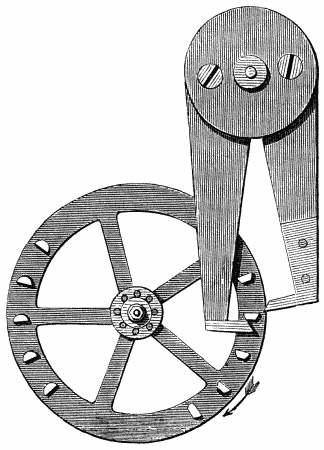
\includegraphics[width=324pt]{images/fig15.png}\label{5spokes}
\label{fig15}
\end{figure}
%-----File: 115.png--------------------------------------------
%-----Folio: 100-----------------------------------------------
\index{Clocks!silent beat}\index{Escapements of clocks!silent}\index{Pallets!silent}%Could not find reference in this page
gets damaged it is easily replaced, whereas if a tooth is
damaged the wheel is ruined. The blow on both pallets
being downwards, the action is more steady than it sometimes
is in the other. The pallets are best made with their
cross section rather convex, and also `half dead.' The scapewheel
of the large clock at King's Cross\index{King's Cross clock}, by which the
Great Exhibition time was kept, and of many others made
from my design, is only $4$~inches wide, with $40$ pins in it.
The lower pallet should be the inner one, and the higher
one outside the wheel, because this makes the action of the
teeth on both of them more direct. If the pallets are on
opposite sides of the wheel with two sets of pins, they may
be alike. The pins must then be at alternate places.

\subsection[Pin pallets.]{Pin pallets.}\markboth{OTHER DEAD ESCAPEMENTS.}{OTHER DEAD ESCAPEMENTS.}\label{subsec:Pin_pallets.}\index{Pallets!pin}\index{Pin pallets}---Some of the best small French clocks now
have an escapement which at first sight may be confounded
with the pin-wheel escapement,
but is really quite different.
The scape-wheel is like a common dead one, and it is set (merely for show) in front of the dial;
but the pallets are
made of semi-cylindrical\label{ruby} ruby pins; the effect of which is
that the half-dead part of the action is not on the points of
the teeth but on their faces. The impulse is the same as on
common jewelled pallets, only with the faces round instead
of flat. I have seen an old clock with similar pin pallets,
made of a thick bristle held at both ends, for the sake of
silence, and the fork also.

\subsection[Single-pin escapement.]{Single-pin escapement.}\markboth{SINGLE-PIN ESCAPEMENT.}{SINGLE-PIN ESCAPEMENT.}\label{subsec:Single-pin_escapement.}\index{Single-pin escapement}\index{Escapements of clocks!single pin}---This very simple and neat-looking
escapement has been several times re-invented. But
I believe the only person who ever made it really succeed,
from better attention to the proportions, was the late
Mr.~C.~Macdowall\index{Dead escapements!Macdowall's}\index{Macdowall's!single-pin escapement}\label{macd}, a very ingenious clockmaker, who died
in 1872 at the age of eighty-two.
There is an interesting
memoir of him in the \textit{Horological Journal} of
Sept.~1873.
But, like many other uneducated inventors, he was very
difficult to convince that an \textit{independent} inventor is not
allowed by the world the credit of a \textit{first} inventor unless he
%-----File: 116.png--------------------------------------------
%-----Folio: 101-----------------------------------------------
is so. He also invented that most useful instrument---the
spiral drill\index{Macdowall's!spiral drill, \&c.}; or rather I should say, he invented the practical
mode of making it by twisting a piece of pinion wire,
\begin{wrapfigure}{o}{126pt}
\caption{\sc Single-pin Escapement}
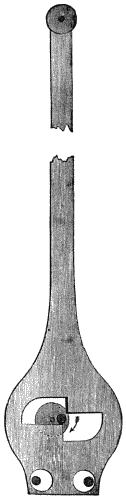
\includegraphics[height=500pt]{images/fig16.png}
\label{fig16}
\end{wrapfigure}
for the thing itself turned up in
wood as an old Indian invention in
the 1851 Exhibition. Another of
his independent inventions was the
`helix lever wheels,' as he called
them, but they also appeared in
some German clocks in the same
Exhibition; besides some other
things which had been published in
well known English books. He also
persuaded himself somehow or other,
that he invented the three-legged
escapement which I shall next describe;
but no one ever saw or heard
of it until it had been made from
my design, though he had shown me
all his inventions, and I had helped
him to get both a patent and an
Exhibition medal for his single pin
escapement, and old Mr.~Dent, under
my advice, had bought the patent
for a considerable sum, and gave
him an order for 500 watches on
that plan if he could make or get
them made, which he could not;
and Mr.~Dent accordingly got some
made in Switzerland. I wore one
of them long enough to see that it
answered very well, but the expense
of the two extra wheels which it
requires overbalanced the advantages,
though I hear they have
%-----File: 117.png--------------------------------------------
%-----Folio: 102-----------------------------------------------
been also made in Paris from Macdowall's instructions,
the patent not having been taken there, and being perhaps
difficult to maintain here if it had been disputed; for the
thing had certainly been published, as we found afterwards
in a French book. Its action is evident enough from this
picture (fig.~\ref{fig16}). It has the advantage of giving a great
part, you may practically say half, of the impulse directly
across the line of centres (of the wheel and pallet arbor)
and therefore with very little friction. The pin is made of
a ruby, and should be set very near the arbor. The older
ones were put too far off. Macdowall made them with a
`neck-bearing,' \textit{i.e.}\ the pivot was behind the wheel, or the
arbor came through the frame, and had the wheel pinned or
squared onto it. The pallet piece itself forms the crutch for
the pendulum, the scape-disc being set behind the clock frame.
It should have eccentric\index{Beat pins!eccentric} fork-pins to adjust for beat.

\subsection[Three-legged dead escapement.]{Three-legged dead escapement.}\markboth{THREE-LEGGED DEAD ESCAPEMENT.}{THREE-LEGGED DEAD ESCAPEMENT.}\label{subsec:Three-legged_dead_escapement.}\index{Three-legged!dead escapement}\index{Dead escapements!Beckett's three-legged}\index{Escapements of clocks!three-legged dead}---It occurred to me\index{Beckett, Sir E.!three-legged dead escapements}
in 1851 that all the best or most direct part of the impulse
in the single-pin escapement might be kept, the more oblique
part got rid of, and one of the extra wheels saved, by using
three pins or teeth instead of one; and the result was this
\begin{figure}[htbp]
\centering
\caption{\sc Three-legged Dead Escapement}
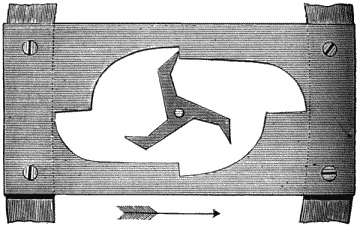
\includegraphics[width=\textwidth]{images/fig17.png}\index{Three-legged!dead escapement}
\label{fig17}
\end{figure}
%-----File: 118.png--------------------------------------------
%-----Folio: 103-----------------------------------------------
\markboth{MY THREE-LEGGED DEAD ESCAPEMENT.}{MY THREE-LEGGED DEAD ESCAPEMENT.}escapement (fig.~\ref{fig17}) (for clocks only, not watches), in which
the upper tooth is shown in the act of giving the impulse.
This is a \index{Scape wheels!a very small one}\textit{full-sized} view of the escapement which drove the
Westminster pendulum of $6$~cwt.\ for half a year, until it
superseded by another modification of it invented for
the purpose of equalising the force of the impulse. That
scapewheel was of steel and weighed only $\frac16$ of an ounce
or $73$~grains, and the clock weight required for it with a
common turret clock movement was only $18$~lbs.\ falling $6$
feet a day, and less than a quarter of what a dead escapement
had required; and considering that more force is lost
by the inertia of such a train than in small clocks, we may
say that the fraction $\frac{\mathrm{W}h}{\mathrm{M}l}$ was less than a third of its usual
amount for the best astronomical pendulums swinging the
same arc. I found also that it was possible to isochronise
the long and short arcs---at least for such variations as
actually occurred, by making the stopping or horizontal
faces half-dead, as I have drawn them. The distance of
the scapewheel from the pallet arbor should be about $24$
times the radius of the wheel, to make it escape at $1^\circ$, allowing
a little for clearance. It requires careful adjustment,
for the greatest depth on the lower pallet is something less
than $\frac18$ of the radius of the wheel.

It is necessary in this and prudent in all dead escapements,
of large clocks especially, to have a spring-fork\index{Forks of pendulums!with springs} to the
crutch; \textit{i.e.}\ the fork-pins attached to the crutch by springs\index{Beat pins!spring},
so that if the scapewheel is not turning from any accident
while the pendulum is moving, and the pallets jam against
the teeth, the fork springs may give way and let the pendulum
go on without breaking a tooth, as it inevitably
will unless so relieved. The pin-wheel escapement is
specially liable to this, because the edges of the pins and
pallets are not sharp as in the common toothed wheel
escapements.
%-----File: 119.png--------------------------------------------
%-----Folio: 104-----------------------------------------------

\begin{figure}[!htbp]
\centering
\caption{\sc Sir E.~Beckett's Three-legged Escapement}
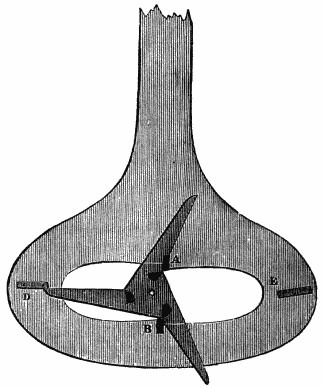
\includegraphics[width=0.9\textwidth]{images/fig18.png}\label{B3leg}
\label{fig18}
\end{figure}
The friction might be still more reduced and the adjustment
of the pallets made easier by making the escapement
with long stopping teeth, as in fig.~\ref{fig18}. It would also
give room for a longer swing of the pendulum, which cannot
safely be made above $2^\circ$ in the other form, or the
stopping faces will reach the scapewheel arbor. An escapement
of this kind clearly reduces the pallet friction to the
smallest amount possible in any dead escapement\index{Beckett, Sir E.!three-legged dead escapements}. It is
however not free from the variations of force in the train.
Constancy of force is only to be got by an entirely different
class of escapements, or by the addition of a train remontoire,
of which I shall speak hereafter under Turret Clocks.

\subsection[Detached escapements.]{Detached escapements.}\markboth{SIR G.AIRY'S DETACHED ESCAPEMENT.}{SIR G. AIRY'S DETACHED ESCAPEMENT.}\label{subsec:Detached_escapements.}\index{Detached escapements!for clocks}\index{Escapements of clocks!detached}---There have been various contrivances
for clock escapements on the chronometer principle
of leaving the pendulum free or detached from the scape-wheel
%-----File: 120.png---------------------------------------------
%-----Folio: 105------------------------------------------------
\begin{figure}[htbp]
\centering
\caption{\sc Sir G.~Airy's Detached Escapement}
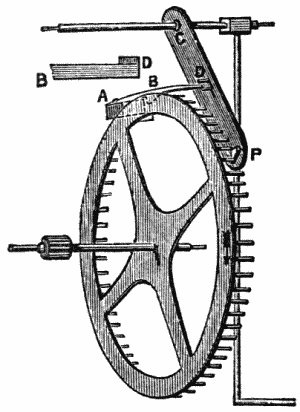
\includegraphics[width=0.5\textwidth]{images/fig19.png}
\label{fig19}
\end{figure}
except at the time of receiving the impulse and of
unlocking the wheel. There is an old French one described
in Rees's Cyclop\ae dia, and Sir G.~Airy\index{Airy, Sir G.~B.!his detached escapement}\index{Detached escapements!G.~B.~Airy's} invented another,
which is described in his before-mentioned Cambridge paper,
and has been lately adopted in the normal sidereal clock\index{Greenwich!sidereal clock escapement, Airy's} at
Greenwich. A few of them had been made before by old
Mr.~Dent, with half-second pendulums, for which this escapement
does not answer, as Mr.~Brock, of George Street,
Portman Square, has also told me. The Greenwich clock\index{Astronomical clocks!Greenwich clock}
however with a seconds pendulum of about $30$~lbs., appears
to answer remarkably well, and therefore I copy the
original picture, from which its action will be easily understood.
The single pallet $\mathrm{CP}$ is exactly like the right hand or
down pallet of a dead escapement.
$\mathrm{ABD}$ is a detent attached to a
fixed block at $\mathrm{A}$ by a slight spring,
$\mathrm{B}$ being the catch which holds
the scapewheel teeth or pins, for
it does not matter which they are.
($BD$ is the flat view of it, omitting
the stop at $\mathrm{B}$.) At $\mathrm{D}$, on the underside
of $\mathrm{ABD}$, there is a very
slight `passing spring' projecting
a little backwards, as shown in
the separate sketch; so that when
\begin{wrapfigure}{o}{100pt}
\hypertarget{fig20}{\caption{\sc Sir E.\ Beckett's Detached Escapement}}
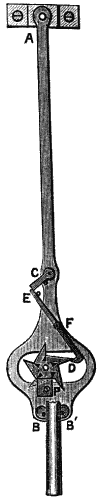
\includegraphics[height=500pt]{images/fig20.png}
\label{fig20}
\end{wrapfigure}
the pin at $\mathrm{D}$ on the pallet goes to
the left it pushes the passing spring
down, and so passes it; but when it comes to the right it
lifts up the detent, because the passing spring being underneath
cannot yield upwards. That unlocks the tooth at $\mathrm{B}$,
and lets another tooth at $\mathrm{P}$ fall upon that pallet, and give the
impulse down its oblique face. The advantages which Sir
G.~Airy contemplated were, the abolition of the dead friction,
and the power of making the impulse begin as much before
zero as it ends after zero, the value of which we saw at p.~\pageref{impulse}.
%-----File: 121.png-----------------------------------------------
%-----Folio: 106--------------------------------------------------

\markboth{SIR E. BECKETT'S DETACHED ESCAPEMENT.}{SIR E. BECKETT'S DETACHED ESCAPEMENT.}But I cannot help thinking the following a better plan
because it gives the impulse without any sensible friction
as  in the three-legged escapement just described, and involves
no passing spring, which is always a delicate arrangement.
I\index{Beckett, Sir E.!detached escapement}\index{Detached escapements!Sir E.~Beckett's} had this clock made and set going in November
1865, and it went till August 1873, nearly 8 years, without
being touched, even with oil, as I wished to see how long
it would go. The arc decreased a little, and it had a slightly
increasing gaining rate in the last few years; but I never
had any clock go so well for anything like that time, though
my gravity escapement clock, to be mentioned presently, has
gone as well for shorter periods. The train is
not a very fine one: with a fine train, or a
coarse one with a remontoire for a turret clock,
I have no doubt this escapement would go at
least as well as any other. But since 1873 it
has not equalled my gravity escapement clocks,
and the gravity escapement is both cheaper and
safer for large clocks than any train remontoire;
which may therefore be considered obsolete.

\hyperlink{fig20}{This figure} shows the construction clearly
enough, except as to size. The locking teeth
of the scapewheel reach about $.6$~in.\ from the
centre, and the impulse pins $.25$~in. Their
centre is $7$~in.\ below the top of the pendulum
and crutch, and the impulse begins about $1^\circ$
before zero, and ends $1^\circ$ after. For the scapewheel
turns $36^\circ$ before and $36^\circ$ after zero;
and therefore, if $r$ is the distance of the pins
from the centre, and $p$ the length of the crutch,
$r\sin 36^\circ$ must $= p \sin 1^\circ$ for an impulse of $2^\circ$;
which makes $p = 3.7r$. Consequently the
dimensions just now given are practically
right, allowing a little for clearance, as you
must. The pallet piece $\mathrm{P}$ is a separate piece of quite
%-----File: 122.png-----------------------------------------------
%-----Folio: 107--------------------------------------------------
hard steel screwed on to the aperture in the crutch $\mathrm{AP}$;
and this requires care in adjustment, as the depth is less
than $\frac15$ of the radius of the wheel, being $r$ \textit{vers.} $\sin 36^\circ$;
which however is more than in the three legs, for this turns
$72^\circ$ at each beat, and that only $60^\circ$, this being a \markboth{SINGLE-BEAT ESCAPEMENTS.}{SINGLE-BEAT ESCAPEMENTS.}single-beat
escapement\index{Beat!single-beat escapements}\index{Escapements of clocks!single beat}\label{singlebeat}\index{Single-beat escapements}, which, it seems necessary to inform some
persons, wastes no power if the train does not move at the
return beat of the pendulum.

But for that it would be better to have no crutch, but make
the action take place on the pendulum itself; it is hardly
possible however to manage that behind a clock of regulator
size, with the pendulum hung to the wall as it should be.
The wheel lies behind the clock in a long cock embracing it
and the crutch. The detent $\mathrm{DEF}$ is on a stud $\mathrm{F}$ in the back
plate, though it looks \hyperlink{fig20}{here} as if it were on the crutch, as the
click $\mathrm{CE}$ really is. When the pendulum goes to the right
(in this drawing) the click trips over the top of the detent,
and when it returns to the left the click pushes the detent
aside, and sets a locking tooth free, and then the \correction{scapewheel} \label{correction4}%**Transcriber's note: The original reads "scrapewheel".
turns and a pin gives the impulse. The shape of the pins
should be observed. It will easily be seen that the scapewheel
should be at the bottom of the clock, and the great
wheel at the top, as in my gravity escapement, and also in
the dead three-legs described at pp.~\pageref{subsec:Three-legged_dead_escapement.} and \pageref{B3leg}.  $\mathrm{BB}'$ are
eccentric beat pins, by which the impulse can be made to
begin as much before zero as you like, so as to make the
angle which we called $\beta$ greater than $\gamma$ if necessary.

\section{REMONTOIRE OR GRAVITY ESCAPEMENTS.}\markboth{GRAVITY ESCAPEMENTS.}{GRAVITY ESCAPEMENTS.}
\label{sec:REMONTOIRE.}\index{Escapements, gravity!theory of}%
\index{Escapements of clocks!remontoire}\index{Gravity escapements}\index{Remontoire escapements}%
These are not to be confounded with the thing called a
train remontoire, which I alluded to just now but shall not
explain till we come to turret clocks, as it belongs only
to them. A gravity or remontoire escapement is one in
which the impulse is not given to the pendulum directly by
%-----File: 123.png--------------------------------------------
%-----Folio: 108-----------------------------------------------
the clock-train and weight, but by some other small weight
lifted up, or a small spring bent up, always through the
same distance, by the clock-train at every beat of the
pendulum. And the great advantage of them is that the
impulse is therefore constant; for the only consequence of
a variation in the force of the clock is that the remontoire
weights are lifted either faster or slower, which does not
signify to the pendulum, as the lifting is always done when
the pendulum is out of the way. If this can be managed
with certainty, and without exposing the pendulum to some
material variation of friction in the work of unlocking the
escapement, which it must perform, its motion and therefore
its time must be absolutely constant, since there is nothing
to disturb it. It does not look a very difficult problem; and
yet it puzzled the clockmakers to solve it in a satisfactory
way for about a century, in consequence of certain small difficulties
which nobody would guess until he had the opportunity
of seeing them in action; and after all it was not done
by the clockmakers, but by two lawyers, in different ways.

But first it may be asked, is the gravity escapement problem
worth solving? Is not the dead or the detached escapement
proved to be good enough both by experience and by
mathematics? The answer is, that in science nothing is
good enough when it can be improved upon: that both
mathematics and experience prove that only by the most
careful and delicate and therefore expensive work, and only
on a small scale and with light weights, can clocks with
`impulse escapements' (\textit{i.e.}\ receiving direct impulse from the
train) be made to go as well as the best of them do; and
although it is possible, by the addition of a train remontoire,
to make even large and heavy dead escapement clocks go
as well as astronomical ones, yet that apparatus involves
not only some extra expense, but what is far more difficult
to provide, some extra attention and intelligence in the
people who have the care of it. We may however dispose
%-----File: 124.png--------------------------------------------
%-----Folio: 109-----------------------------------------------
of a great number of the contrivances for gravity escapements
by the remark, that they require not less, but more
delicacy of construction and careful handling afterwards than
the finest dead escapement, even if they `perform' any
better, which scarcely any of them do.

Before we can appreciate the merits and the difficulties of
this class of escapements, it is clearly necessary to understand
the theory\index{Gravity escapements!theory of} of them; which I shall be able to exhibit more
briefly than that of the dead escapement, as some of the
ground is common to them both, and especially that useful
formula of Sir G.~Airy's for the variation of the time caused
by any escapement, from which I shall start again. But it
will help our conception of the process if we first take some
simple form of gravity escapement as an illustration of
their principle; and it does not signify that that form was
neither the first nor the best, on account of certain mechanical
objections which we are not concerned with yet.

\subsection[Mudge's gravity escapement.]{Mudge's gravity escapement (Fig.~\protect\ref{fig21}).}\markboth{MUDGE'S GRAVITY ESCAPEMENT.}{MUDGE'S GRAVITY ESCAPEMENT.}\label{subsec:Mudge's_gravity_escapement.}\index{Gravity escapements!Mudge's}\index{Mudge!his gravity escapement}---The pallets $\mathrm{AC}$, $\mathrm{BC}$,
are no longer fixed on one arbor, but on two, as close to the
bend of the pendulum spring as possible. The acting faces
are so shaped and placed that whenever the wheel moves
from $\mathrm{B}$ towards $\mathrm{A}$, a tooth will lift one of them until it is
stopped by the nib $a$ or $b$ at the end of each acting face.
Here the pallet $\mathrm{A}$ has just been lifted and is holding the tooth
that lifted it; as soon as the pendulum comes, moving to the
right, it will evidently push that pallet out of the way by
means of the fork-pin $\mathrm{P}$, and so free the tooth, and the wheel
will begin to turn, and the opposite tooth will immediately
lift the pallet $\mathrm{B}$ till it likewise is stopped by $b$. The pendulum
is all the time going on rising to the right and carries the
right pallet with it as far as it likes to go; when it begins to
fall the pallet falls with it, not only to the place where it was
taken up, but to a lower place, corresponding to that of the
left pallet in the picture; and the fall of the weight of the
pallet from the place where it is taken up by the pendulum
%-----File: 125.png--------------------------------------------
%-----Folio: 110-----------------------------------------------
to the place where the pendulum leaves it, or the difference
between its rise and fall with the pendulum, constitutes the
impulse, and that difference is evidently constant, however
far the pendulum may swing.\par
\begin{figure}[htbp]
\centering
\caption{\sc Mudge's Gravity Escapement}
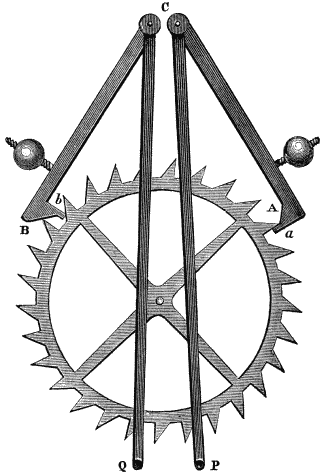
\includegraphics[height=0.8\textheight]{images/fig21.png}
\label{fig21}
\end{figure}
If the weight of the pallets were partly or wholly counterbalanced,
and they were fixed by springs instead of acting by
their own weight on pivots, it could no longer be called a
gravity escapement, but would have the more general French
%-----File: 126.png--------------------------------------------
%-----Folio: 111-----------------------------------------------
name of a remontoire; but the principle would be the same,
except that the force of the springs has a law of its own, and
is more variable than that of gravity.

It is easy to show that the effect of a gravity escapement
is to make the pendulum go faster than a free pendulum, by
exactly the same reasoning as was used to contrast the dead
and the recoil escapements; or still more simply, by considering
that the remontoire weights are in effect so much
weight added to the pendulum far above its centre of oscillation
and therefore they accelerate it. But this tells us
nothing about the variation of the rate, in case the arc increases
or decreases a little under any change of friction;
and we shall see presently that a very curious result comes
out with respect to this, which it is impossible to arrive at
except by calculation.

\markboth{MATHEMATICAL THEORY OF GRAVITY ESCAPEMENTS.}{MATHEMATICAL THEORY OF GRAVITY ESCAPEMENTS.}To do this we must find out again what that quantity
called $\phi$ in Sir G.~Airy's\index{Airy, Sir G.~B.!for gravity escapements}\label{gairycalc2} formula at p.~\pageref{gairycalc}, is for this escapement.
Let the angle after zero at which the pendulum begins
to lift the pallet be called $\gamma$, and the angle at which it leaves
the other pallet which has been giving the impulse $\pm\beta$, according
as that takes place after or before zero: so that, as
in the dead escapement, the angle $\gamma+\beta$ is the angle of
impulse, if the descending pallet is left after zero, which we
shall see is the best arrangement. Let $\mathrm{P}g$ be the weight of
each pallet, and $p$ the distance of its centre of gravity from
its axis at $\mathrm{C}$, and $\delta$ the angle which $p$ makes with the
pendulum when they are in contact. $\mathrm{M}l^2$ represents the
moment of inertia of the pendulum as usual; strictly speaking
we ought to add to it the moment of inertia of the
pallets while they are in contact with the pendulum; but as
that makes no difference in the nature of the result, and in
the best escapements one pallet or the other is always in
contact, we may either consider that as included in $\mathrm{M}l^2$ or
neglect it altogether. Then the equation of motion will be
\[
\frac{d^2\theta}{dt^2}=-\frac{g\sin\theta}{l}-\frac{\mathrm{P}pg\sin(\delta+\theta)}{\mathrm{M}l^2}.
\]
%-----File: 127.png---------------------------------------------
%-----Folio: 112------------------------------------------------
We may put $\theta$ for $\sin \theta$ and $1$ for $\cos \theta$ ($\theta$ being small),
\[
\therefore \frac{d^2 \theta}{dt} =-\frac{g\theta}{l} \left(1+\frac{\mathrm{P}p}{\mathrm{M}l}\right)-\frac{\mathrm{P}pg\sin \delta}{\mathrm{M}l^2}.
\]

This is of the same form as in the dead escapement;
only here the constant term involving simply $\theta$, which
always indicates isochronism, has its coefficient increased;
which shows that the pendulum will regularly go faster than
if its own gravity alone acted upon it, exactly as it is accelerated
by those small regulating weights which I described
at p.~\pageref{smallweights}. The other term constitutes the disturbing force $\phi$,
from which we are to learn what will be the disturbance of
the isochronism if the arc varies a little; and this result will
also be of the same form as before, except that the limits of
$\phi$ are different, as it does not act now through the middle of
the arc only, but from $-\alpha$ to $\beta$ and from $\gamma$ to $\alpha$; and even
if $\beta$ should be identical with $\gamma$ the action is not continuous
for the falling pallet pushes the pendulum from $-\alpha$ to $\beta$,
but the pendulum lifts the pallet from $\gamma$ up to $\alpha$. Therefore
the result of the integration will be (putting $\mathrm{W}h$ for the sum
of $\mathrm{P}p\sin \delta$ for the whole day):
\[
\Delta\mathrm{T} =-\frac{\mathrm{W}h(\sqrt{\alpha^2-\gamma^2}+\sqrt{\alpha^2-\beta^2})}{\mathrm{M}l\pi \alpha^2(\gamma+\beta)};
\]
which differs from the dead escapement formula only in the
signs; but we shall see that that produces another very important
difference. First however we may remark that if
$\beta$ is $-$ (that is, if the falling pallet is left before zero), or
even if it is smaller than $\gamma$ (and it cannot be larger with
safety to the locking), $\Delta\mathrm{T}$ is increased, and so will all its
variations be when there are any. Therefore let us assume
that $\beta$ is as large as it can be, \textit{i.e.}\ that one pallet is taken up
just when the other is left, or $\beta=\gamma$; and then the formula
becomes much more simple:
\[
\Delta\mathrm{T} =-\frac{\mathrm{W}h}{\mathrm{M}l\pi \alpha^2} \sqrt{\frac{\alpha^2}{\gamma^2}-1}
\]
%-----File: 128.png-----------------------------------------------
%-----Folio: 113--------------------------------------------------
We must differentiate this, as before, to see what the
variation of rate will be; but this time we need not consider
$\mathrm{W}$ or the force of the impulse variable, because we know it
is not---if the escapement is what it pretends to be. Then
\[
d\Delta\mathrm{T} = \frac{\mathrm{W}hda \frac{\alpha^2}{\gamma^2}-2}
{\mathrm{M}l\pi\alpha^3\sqrt{\frac{\alpha^2}{\gamma^2}-1}}
\]

From which this remarkable result appears,---that if the
weight of the pallets is so adjusted that the pendulum swings
through an arc $\alpha = \gamma\surd{2}$, the rate will not vary at all, even
when the arc does, except what may be due to the circular
error. Unfortunately they both have the same sign, and
therefore the escapement cannot be made to correct the
circular error\index{Circular error of pendulum}. But there happens to be a mechanical
difficulty in making $\gamma$ as large as $\frac{\alpha}{\surd{2}}$
or $.71\alpha$, which would
be $85'$ if $\alpha = 2^\circ$; and moreover Mr.~Bloxam\index{Bloxam!his escapements} came to the
conclusion, as stated in his papers, that from other causes,
especially the variation of density of the air, it is better
to make $\gamma$ considerably smaller than $.71\alpha$. Let us see
then what the variation of rate from the escapement will
be for some such value of $\gamma$ even as far from the theoretical
value as $\frac{\alpha}{4}$.


In the Westminster clock I know by trial that $\frac{\mathrm{W}h}{\mathrm{M}l}$ at the
escapement is not more than $\frac{1}{45}$; taking it at that, and $\alpha$ at
$2^\circ\ 40'$, as it is, and $\gamma =\frac{\alpha}{4}$, you will see, if you take the
trouble to make the calculation, that the clock will only gain
about a second a month for a decrease of arc of $5'$, which is
larger than is likely to happen, besides what is due to the
circular error so far as it is uncorrected by the spring.
%-----File: 129.png---------------------------------------------
%-----Folio: 114------------------------------------------------

In those escapements where the falling pallet is left before
zero, the expression for the variation of rate would be
\[
d \Delta\mathrm{T} = \frac{\mathrm{W}hd\alpha}{\mathrm{M}l\pi \alpha^3(\gamma-\beta)} \left\{\frac{\alpha^2-2\gamma^2}{\sqrt{\alpha^2-\gamma^2}}+\frac{\alpha^2-2\beta^2}{\sqrt{\alpha^2-\beta^2}}\right\}
\]
in which you observe $\gamma-\beta$ instead of $\gamma+\beta$ is in the
denominator, and therefore the variation is much larger than
in the other form of the escapement. Theoretically indeed
this might also be made $= 0$ by making the three angles
satisfy this condition,
\[
\sqrt{\alpha^2-\gamma^2}\sqrt{\alpha^2-\beta^2} = \frac{\alpha^2}{2}.
\]

\label{conclusion}Thus $\gamma = 90^\prime$ and $\beta = 78^\prime$ would be right for $\alpha=2^\circ$;
but these small differences would be even more inconvenient
mechanically than $\gamma = 85^\prime$ in the other case. That construction
therefore is decidedly the worst, notwithstanding
the tempting appearance of the pendulum being left free
through the middle of its arc; a fact which would probably
never have been known with certainty without this kind
of investigation, as the errors would have been sure to be
attributed to any but the right cause.

Reid mentions, at page~139 of his old book, a curious fact
bearing on this. He says he cut a hole in the side of the case\label{closecase}
of a gravity escapement clock, which increased its arc from
$1^\circ~22^\prime$ to $1^\circ~37^\prime$, and at the same time made it gain $42$~sec.\ a
day, and a larger hole increased the arc $12^\prime$ more, and I
suppose the rate. Therefore the diminished resistance, from
the pendulum being able to drive the air before it through the
hole, much more than counteracted both the circular error
and the escapement error, making the clock gain this great
amount instead of losing a little under the increased arc.
Moreover such an enormous variation of rate as this shows
that the motion of the air in the clock-case may affect the
%-----File: 130.png-----------------------------------------------
%-----Folio: 115--------------------------------------------------
rate materially. But I must add that I have twice tried the
experiment myself in a still stronger way, by taking off the
clock case altogether from my own gravity escapement clock,
and I could not observe any increase of arc at all---certainly
not of $5'$, nor any alteration of rate. The arc was however
nearly $1^\circ$ larger than in Reid's clock before he cut the holes;
and this is another proof of the unsteadiness of very small
arcs I have since found that a small enclosure for a turret
clock pendulum bob did diminish the arc a little.

Probably no one would foresee, without experiment, that
the simple form of escapement in p.~\pageref{fig21} would fail\markboth{FAILURE OF EARLY GRAVITY ESCAPEMENTS.}{FAILURE OF EARLY GRAVITY ESCAPEMENTS.}\label{failure}. Several
of the most elaborate French turret clocks in the Exhibition
of 1851 were on that plan, and people were very much
surprised when I showed them that you could make all those
clocks increase their arc visibly and speedily by increasing
the clock-weight, which is directly contrary to the fundamental
principle of a gravity escapement. This form of the
escapement was invented by Mudge, a celebrated watchmaker
whom I shall have to mention again, and it had long been
known here that it would not answer, on account of its liability
to \textit{trip}, or to have the pallets jerked out so far by the
motion of the wheel that the nib fails to catch the lifting
tooth, and so three or four teeth run past and the time is
altogether lost. The only way of avoiding this liability is to
use a very highly finished train with high numbered pinions
to keep the force uniform, and then to make that force only
just enough to raise the pallets; but that is inconsistent
with the clock being able to work anything but a small dial,
and if it is not kept very clean and the oil fresh, it will be
sure to stop. In short, the clock becomes too expensive and
delicate, and requires too much attention to be tolerated in
common use.

\subsection[Cumming's escapement.]{Cumming's escapement.}\markboth{CUMMING'S AND HARDY'S ESCAPEMENTS.}{CUMMING'S AND HARDY'S ESCAPEMENTS.}\label{subsec:Cumming's_escapement.}\index{Cumming's escapement}\index{Escapements, gravity!Cumming's}---But even if all these risks
were got over, there is still another radical defect in all such
escapements, which does not appear to have been ever
%-----File: 131.png---------------------------------------------
%-----Folio: 116------------------------------------------------
noticed before I pointed it out with reference to those clocks
in the Exhibition. The force may easily be enough to raise
the pallets a little too high, without jerking them over the
tooth altogether, and then the pressure on the nib is quite
enough to keep them there, and so the pallet is taken up by
the pendulum at some angle greater than the proper one $\gamma$;
and as it falls down with the pendulum to a constant place,
the impulse lasts longer than it ought, and of course the arc
is increased. I gave the name of \textit{approximate tripping} to this
defect, and any escapement which is liable to it is evidently
worth nothing. It seems capable of happening even where
the impulse or sloped portion of the pallet is put on one arm
and the nib on a separate one which is not lifted at all by the
wheel, but only by the pendulum, as in Cumming's escapement,
which was invented very nearly a century ago, and
for a time was thought to answer well. I suppose this is
in consequence of the force with which the tooth strikes the
stop pallet, sometimes throwing it a little out of its place,
unless it is undercut or given a slight recoil the wrong way;
and that is objectionable too, because it resists the unlocking,
and does not always resist with the same force.

\subsection[Hardy's escapement.]{Hardy's escapement.}\markboth{HARDY'S ESCAPEMENT.}{HARDY'S ESCAPEMENT.}\label{subsec:Hardy's_escapement.}\index{Escapements, gravity!Hardy's}\index{Hardy's escapement}---One of the objections to Cumming's
escapement was the friction of no less than $8$ pivots
of the $4$ arms which had to move with the pendulum in the
course of each vibration. Hardy avoided this by setting the
arms on springs instead of pivots; but that introduced
another and probably a worse evil, because the stiffness of
the springs varies with the temperature, which of course
disturbs the rate of the pendulum. That escapement was
consequently removed from the transit clock at Greenwich
many years ago, and a dead one substituted. There were
some very good rates of three Hardy's clocks published in
\textit{Pearson's Astronomy}; but they are practically extinct.

\subsection[Kater's escapement.]{Kater's escapement.}\markboth{KATER'S AND OTHER GRAVITY ESCAPEMENTS.}{KATER'S AND OTHER GRAVITY ESCAPEMENTS.}\label{subsec:Kater's_escapement.}\index{Escapements, gravity!Kater's}\index{Kater!his escapement}---The late Captain Kater, who paid
great attention  to  the  theory of pendulums, invented a
%-----File: 132.png-----------------------------------------------
%-----Folio: 117--------------------------------------------------
gravity escapement, which is very fully described in the
130th\ vol.\ of \textit{Philosophical Transactions}, on the principle of
making the weight of the descending pallet unlock the scape-wheel
by falling upon an anchor like a pair of dead escapement
pallets without the impulse faces. He supposed that
as the inertia of the anchor would stop the pallet for a
moment, the pendulum would leave it there, and so be itself
free from the friction of unlocking. But here again it was
found that the force of the wheel was apt to displace the
anchor unless its pallets were undercut, and then the resistance
was sometimes too great for the gravity pallets to
overcome, unless they were too heavy for the pendulum;
and after many attempts to make it go, that escapement
also was taken out of the only clock to which I know of it
being applied, and came into the hands of Mr.~Bloxam, who
showed me it. The failure of it is described in his paper
before mentioned.

\subsection[Gowland's escapement]{Gowland's escapement}\markboth{GOWLAND'S ESCAPEMENT}{GOWLAND'S ESCAPEMENT}\label{subsec:Gowland's_escapement}\index{Escapements, gravity!Gowland's}\index{Gowland's escapement}, which was in the Exhibition of
1851, was on the same principle as to the unlocking only.
He had not even pallets for the impulse, but a pair of small
weights, which hung on long arms or spikes projecting horizontally
from the locking pallets, except when they were
lifted off by similar arms projecting from the pendulum.
This prevented the friction of any pallet pivots affecting the
pendulum. The locking pallets were of Mudge's form, and
were prevented from being driven too quickly and tripping,
by paddles descending from them into a pot of oil---not a
very elegant contrivance certainly, and requiring a good deal
of extra force in the train. I heard no more of it after the
Exhibition, at which I was not surprised.

\subsection[M.~Gannery]{M.~Gannery}\markboth{M.~GANNERY}{M.~GANNERY}\label{subsec:M.Gannery}\index{Escapements, gravity!Gannery's}\index{Gannery's escapement}, of Paris, had an escapement there also, on
the same principle as to the small weights, which were hung
by strings from the pallet arms and received in cups on the
pendulum arms, or \textit{vice vers\^a}. But instead of the oil pot, he
made the scapewheel of the usual size with only $9$ teeth of
%-----File: 133.png--------------------------------------------
%-----Folio: 118-----------------------------------------------
very slow rise and a nib at the end, which therefore lifted
the pallets slowly and seemed to obviate the tendency to
trip, so far as I could judge by merely looking at it. I
should think however that the rigidity of the strings would
be quite enough to affect the pendulum, and the friction in
lifting was considerable. Moreover I doubt whether the
stopping of the unlocking weight in any of this class of
gravity escapements is decisive enough to make the difference
of the angles of lift and of drop quite constant; and if it is
not the escapement fails. Of that escapement also I heard
no more, and the French members of the jury evidently
thought very little of it. Nevertheless, the scapewheel with
$9$ teeth instead of $30$, which reduces the pressure of the stops
in that proportion, was a great advance in the right direction
though not absolutely new, because the same thing had been
done much better some years before in

\subsection[Bloxam's escapement.]{Bloxam's escapement.}\markboth{FORMER GRAVITY ESCAPEMENTS.}{BLOXAM'S ESCAPEMENT.}\label{subsec:Bloxam's_escapement.}\index{Bloxam!his escapements}\index{Escapements, gravity!Bloxam's}---This is so superior to the
others that it deserves a more particular description. This
drawing (\hyperlink{fig22}{next page}) of the full size in Mr.~Bloxam's own
clock, is copied (with a little alteration for distinctness of
exhibition) from his account of it in the Astronomical
Society's Memoirs of 1853. The pallets are lifted alternately
by the small wheel or pinion with $9$ teeth, and with
scarcely any friction, as the action is only for a short distance
across the line of centres. The stopping is done by
the long teeth, and the pressure there is less than the lift in
the proportion of the radii of the small and large wheels.
The stops are $\mathrm{A}$ and $\mathrm{B}$: $\mathrm{E}$ and $\mathrm{F}$ are the fork pins which
embrace the pendulum. The pallets above at $\mathrm{C}$ are cranked,
that their centres of motion may be identical with that of
the pendulum; which is perhaps an unnecessary refinement,
especially as the pendulum spring has no one centre of
motion. The size of the wheel determines that of the pallets,
thus: if the radius of the wheel is $1$~in.\ the length of each
pallet down to the stop must be $2.8$~in., to make the angle
%-----File: 134.png--------------------------------------------
%-----Folio: 119-----------------------------------------------
between the locking teeth and each pallet $90^\circ$. Mr.~Bloxam
made the angle $\gamma$, at which the pendulum leaves one pallet
and takes up the
other, only $20^\prime$ in
his clock, and $\alpha =
1.^\circ 40^\prime$, these being
the proportions
which he concluded
were the best to
counteract the effect
of variations of density
of the air.
\begin{figure}[htbp]
\centering
\hypertarget{fig22}{\caption{\sc Bloxam's Gravity Escapement}}
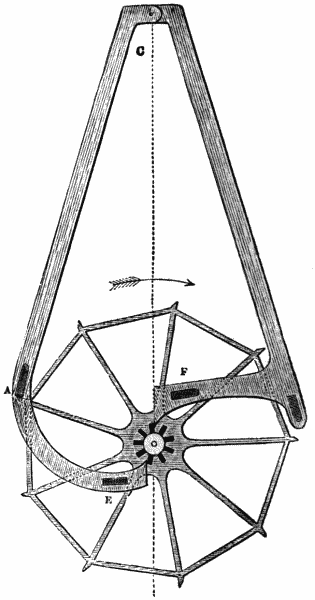
\includegraphics[height=0.8\textheight]{images/fig22.png}
\label{fig22}
\end{figure}

The objections to
this escapement are,
that it is delicate and
expensive to make,
both in itself and in
the rest of the clock,
and if a pallet got
accidentally lifted
the wheel would run
with great velocity
and probably break
a tooth when the
pallet stopped it
again---an evil to
which most of the
previous escapements
are equally
liable, and it is a
very serious one.
It is also liable to trip unless the train is very fine,
so that no more weight need be used than is absolutely
necessary. But unless a gravity escapement will enable the
clock to do with a coarse train, it is of no real use; at any
%-----File: 135.png--------------------------------------------
%-----Folio: 120-----------------------------------------------
rate it is quite certain not to come into use; and Mr.~Bloxam
said that he  considered a fine train essential. That in his
own clock was the finest and had almost the highest numbered
pinions (18) I ever saw. And therefore after all, this
can only be regarded as a theoretical or scientific solution of
the gravity escapement problem, but hardly a practical one.
I expressed this opinion of it in early editions of this book
and stated that old Mr.~Dent and I had agreed that it would
not do for the Westminster clock,  even if protected from
variations of force by a remontoire in the train. Somebody
however thought  he knew better; for in the 1862 Exhibition
there appeared for a short time a small turret clock
with this escapement, and a train remontoire, which was
said in the newspapers to have been made under the direction
of the Astronomer Royal. But it could not be made to
behave properly, and after a few weeks was withdrawn.

At the same time, Mr.~Bloxam\index{Bloxam!corrected Sir G.~Airy} deserves the credit of
having first discovered, though he did not publish the
discovery till long afterwards, that the practical conclusions
of Sir G.~Airy's Cambridge paper were \label{gairyerr2}erroneous; and that
the errors of a dead escapement cannot be made either insignificant
or constant; that the dead friction does not
correct itself before and after zero; that the acceleration of
a gravity escapement pendulum over a free pendulum does
not signify the least; but that what does signify is the
constancy of that acceleration; and that the variation is
least when the acceleration is greatest, and may be made
practically nothing by a particular arrangement of the angles
of impulse. The Astronomer Royal afterwards in effect
assented to all this, first by admitting in 1852 that my
gravity escapement, which will be described presently,
answered perfectly, and by himself communicating to the
Royal Astronomical Society Bloxam's two papers of 1853
and 1858 sent from Madeira, the latter of them after he was
dead; and then actually going too far and assuming that
%-----File: 136.png--------------------------------------------
%-----Folio: 121-----------------------------------------------
Bloxam's escapement was a practical solution of the gravity
escapement problem.

\subsection[Sir E.~Beckett's Gravity Escapements.]{Sir E.~Beckett's Gravity Escapements.}\markboth{SIR E.~BECKETT'S GRAVITY ESCAPEMENTS.}{SIR E.~BECKETT'S GRAVITY ESCAPEMENTS.}\label{subsec:Sir_E.Beckett's_Gravity_Escapements.}\index{Beckett, Sir E.!four and three legged gravity escapements}\index{Escapements, gravity!Beckett's|(}\index{Gravity escapements!Beckett's four-legged}---I have now
to describe the only escapements of this kind which have ever
come into real use; and that both for large and astronomical
clocks, especially the former. The earliest form of them
need no longer be described, as it has been superseded by
two others, one with a four-legged scapewheel for small
clocks, and the other with a double three-legged wheel for
large ones.

\subsection[The four-legged escapement]{The four-legged escapement}\markboth{THE FOUR-LEGGED ESCAPEMENT.}{THE FOUR-LEGGED ESCAPEMENT.}\ \label{subsec:The_four-legged_escapement}\index{Four-legged gravity escapement}is shown in \hyperlink{fig23}{this drawing}
of a regulator of this kind seen from behind, half the real
size. To avoid confusion, only the centres of most of the
wheels are shown, and you see the train is inverted, to save
height in the frame and clockcase. $\mathrm{G}$ is the great wheel
arbor, and the barrel is shaded; $\mathrm{C}$ the centre wheel, close to
the top of pendulum and pallet arbors, $\mathrm{B}$~second wheel,
$\mathrm{A}$~seconds-hand wheel, and $\mathrm{E}$ scapewheel. $\mathrm{DD}$ are the
brackets which come out of a large cast-iron plate or back,
from which also comes the pendulum cock, shown by
partly broken lines, to leave the pallet cock visible. $\mathrm{PP}$ are
the pillars, $\mathrm{CST}$, $\mathrm{CS}^\prime\mathrm{T}^\prime$ the pallets, and their inside pivots
(the arbors being very short) run in a flat piece or cock
between the centre wheel and the clock plate or frame.
The scapewheel speaks for itself as to the long locking
teeth; but it has two sets of lifting pins near the centre,
pointing alternately backwards and forwards, one set lifting
one pallet and the others the other, the pallets being in
different planes, before and behind the wheel, with one stop
$\mathrm{S}$ pointing forwards and the other $\mathrm{S}^\prime$ backwards. This cannot
be done otherwise with an even-numbered wheel, and
though it can with a five-legged one, that is an inferior
construction in other respects, and is much more difficult
to make rightly, and has not one advantage when it is
made. I say this from experience now, as I did before
%-----File: 137.png--------------------------------------------
%-----Folio: 122-----------------------------------------------
\begin{figure}[p]
\centering
\hypertarget{fig23}{\caption{\sc Four-legged Gravity Escapement}}
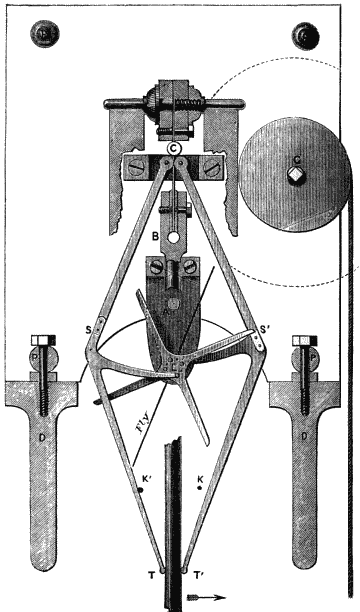
\includegraphics[height=0.9\textheight]{images/fig23.png}
\label{fig23}
\end{figure}
%-----File: 138.png--------------------------------------------
%-----Folio: 123-----------------------------------------------
from theory. For with the strange propensity of mankind
for taking more trouble to do wrong than it would take to
do right, some persons would persist in making the escapement
with five legs. I thought it might possibly save a
little force or weight on the train, but it does not even do
that; nor anything else, except give more trouble to adjust:
whereas the four-legged one is so easy that the very first I
had made went at once perfectly without any alteration.

The great feature of them is the regulation of the velocity
and the avoidance of the banging on the pallets and the risk
of tripping, either actual or approximate, by putting a
common fan-fly on the scapewheel arbor. And this
becomes possible or effective only by reason of the large
motion of the wheel and fly\index{Fly, striking!for gravity escapements} at every beat: viz.\ $45^\circ$ in this
escapement, and $60^\circ$ in the three-legs. A fly would be of
very little use in Bloxam's escapement, to say nothing of
its other difficulties. In order to leave room for the fly
the seconds-wheel arbor is cut short and set in a cock within
the frame, which leaves space enough for a fly above $2$~in.\ long
in each arm, from $\mathrm{E}$ to $\mathrm{B}$.

\markright{PROPER CONSTRUCTION.}The pallets require no beat screws, as they are only thin
pieces of steel like square wires, which can easily be bent
for adjustment; and even for a $40$~lbs.\ pendulum they
have to be made very light; they must be cut out of steel
plate, and the lifting faces hardened. The pins are found to
do better also of steel than of brass, and one set of them
should be tapped into the wheel with left-handed screws, so
that the action of lifting may not tend to loosen them. The
wheel is either screwed on the arbor up to a shoulder with a
left-handed screw, so that the action tends to tighten it, or
is `squared on' a hexagon and pinned. The scapewheels
are also generally cut out of thin steel plate; but some have
been made of a harder kind of gun-metal or softer kind of
bell-metal, and I am not certain which is best. But in either
case the stops must be as hard as possible, either steel quite
%-----File: 139.png---------------------------------------------
%-----Folio: 124------------------------------------------------
hard or jewels. I think steel hard enough, and I do not
believe in leaving any place where there is friction totally
dry, though the oil may be the least possible.

Another great advantage of these escapements is that the
length of the teeth or legs, and the largeness of their motion,
make the pressure on the stops, or the work of unlocking
by the pendulum, insensible; and therefore also they are
incapable of holding up the pallets so as to cause `approximate
tripping' by any force that you can apply to the great
wheel, provided the escapement is made properly.  But
with that same genius for doing things wrong when it
is as easy to do them right, some persons have made the
angle $\mathrm{CSE}$, at the stop which is struck upwards, less than
$90^\circ$, and then have said the escapement failed because
it sometimes tripped, as it was pretty sure to do. For
safety it is as well to put the up stop a little higher, and the
down stop a little lower than their proper theoretical places,
which are where both the angles would be exactly $90^\circ$.

That determines the theoretical distance of the pallet
arbors $\mathrm{C}$ from $\mathrm{E}$ the scapewheel centre. If its diameter is
$4$~in.\ that distance is $5.2$, and that \textit{is} the proper distance of
the top of the pendulum spring above $\mathrm{E}$\@. The pallet arbors
must evidently be a little lower. Mr.~Bloxam made them
cranked (see p.~\pageref{fig22}) in order to get their common axis in a
line with the top of the spring; but that is an unnecessary
refinement, at least for these escapements, and is never done.
And as no point in the pendulum really swings quite in a
circle, I doubt if the friction of the pallets on it would be
sensibly less for their being both made to describe the same
circle by cranking their arbors: at any rate it is too insignificant
to care about.

The distance of the lifting pins from the centre should not
be more than a $40$th of $\mathrm{EC}$, or else the angle of impulse $2\gamma$
will be larger than is found expedient. It is difficult to
make the pallets light enough even with a small $\gamma$ and the
%-----File: 140.png-----------------------------------------------
%-----Folio: 125--------------------------------------------------
larger it is the lighter they must be. The length of their tails
down to the beat pins is arbitrary, but I found the Westminster
clock perform decidedly better with the pallet tails
long than short. The length \hyperlink{fig23}{here shown} does very well,
and it looks neat to make the two parts reciprocally parallel.
The pins should be placed so that the lifting may take place
equally across the line of centres $\mathrm{CE}$, because then it is
done with the least friction. For this purpose the pins
which lift the lower pallet must be set on the radii which
run along the acting faces of the teeth, and the other set of
pins half way between them, with reversed screws, as I said
before.

\markboth{FOUR-LEGGED ESCAPEMENT.}{FOUR-LEGGED ESCAPEMENT.}Any gravity escapement requires a heavier\index{Gravity escapements!require heavy weights} weight than a
dead or detached one, other things being equal, because it
must be strong enough to lift the pallets promptly and
firmly always; but the superfluous force does not reach the
pendulum, and therefore does no harm, provided the train is
good enough not to waste much force generally in order to
get over occasional weak places from bad wheel-cutting.
Nothing tests the defects of a train like a gravity escapement.
If there are bad places in a common clock train they must
be very bad indeed for the teeth not to follow the pallets,
though they may be giving no effective impulse for some
seconds; but in a gravity clock the pallets have always to
be lifted; and I have never got a train yet in which I could
not hear some weak place, recurring always at the same time
of day, and requiring at least an extra pound in the weight
beyond what was generally wanted. For that reason,
though a high numbered train is not, or ought not to be
requisite for these clocks, it should be a thoroughly good
one; and as defects of cutting affect low numbers more than
high ones, it is better to have them rather high, though they
need not be anything like what are used for first-rate dead
escapements. I have the upper pinions of $10$ and the centre
one of $12$, and if these are well cut, and still better if they
%-----File: 141.png-----------------------------------------------
%-----Folio: 126--------------------------------------------------
are lantern pinions, they are enough; if they are not, you
will soon hear and see it by the escapement, and the train
should be rejected as a bad one.

In gravity regulators, for the same reason, the wheel must
have a little run at the pallets before it begins to lift them
just as many clocks will not begin to strike if the hammer
tail lies on the pins: \textit{i.e.}, there must be banking \label{banking}pins $\mathrm{KK}'$
for the pallets to rest on just clear of the lifting pins. And
in turret clocks the banking pins are useful to reduce the are
without making the pallets too thin. They may be simply
a thin piece of metal adjusted for the beat pins to fall on.

It is better to have a full-sized barrel with three lines and a
fixed pulley for a `three-quarter length' clock than two
lines and a smaller barrel. A clock of this kind with a
$40$~lbs.\ pendulum swinging $2^\circ$ requires a weight of from $20$
to $24$~lbs., according to the train, to lift the pallets promptly
and firmly, and loud enough for an observer.

These clocks have also been made to strike a small bell
every minute by a pin on the minute wheel, which enables
an observer to go on for some time without looking at the
clock. Of course this requires rather more weight, and no
such extra friction could be tolerated in a dead escapement.
My clocks strike one at the hour on a rather large bell, but
that makes no sensible difference in the weight. When
there is a full striking part, the train must be arranged in the
usual position, which is inverted in the mere going clocks, to
save unnecessary height of the frame and the pendulum
being several inches above it, on account of the extra wheel
and the length of the pallets. The great wheel is also put
on the left side to keep it near the side of the case and out
of the way of the pendulum. When a pendulum imparts
vibration to the weight, as they do sometimes, the simplest
cure for it is to put a board down the side for the weight to
graze when it is near the pendulum. It has never happened
in my clocks, and three lines tend to prevent it.
%-----File: 142.png-----------------------------------------------
%-----Folio: 127--------------------------------------------------

Unfortunately I have no daily rate of any of these clocks
regularly taken in an observatory\index{Astronomical clocks}\index{Clocks!astronomical}, until we come to the
largest of them all; but judging of my own for long periods
by the Westminster clock, which is tested daily, I have no
difficulty in pronouncing it superior in steadiness of rate to
any dead escapement whose rate I have ever seen. And
they are made by Mr.~Brock, of George Street, Portman
Square, and I dare say by other makers, for half the price of
the old-fashioned best dead escapement regulators with only
$12$~lbs.\ pendulums.

\markboth{SIRE E. BECKETT'S GRAVITY ESCAPEMENTS.}{INFERIOR MODIFICATIONS.}Some persons have taken a great deal of unnecessary
trouble to modify these escapements in order to avoid the fly,
as if that did any harm; and have added train remontoires,
as if that did any good to any gravity escapement which
really is a gravity escapement---\textit{i.e.}\ which has no tendency
to trip, and gives a constant impulse clear of the friction of
the train. One of these attempts to get rid of the fly was
exhibited by Dr.~Clark in 1862; but the wheel was stopped
with a bang that thrilled all through the clock, which only
tends to knock it to pieces, and keeps everything in a state
of vibration. It was also a much more delicate construction,
and I should prefer Bloxam's if I had to choose between
them; for if you have not a fly, the less the motion is at
each beat the better. Another contrivance for the same purpose,
invented by a French workman here, was used by his
employers in a few church clocks, and then abandoned, and
my original form resumed by the makers in all their turret
clocks. The fly\label{fly} should of course be as light as possible,
either of thin steel or aluminium; and the best way to put it
on is with a piece of watch spring pushed in through an
oblong hole so as to press always on the arbor, which
should \textit{not} be very thin. Some persons do not seem to
know that a long fly is more effective than a wide one of the
same area.

Another mistake made by several of these inventors,
%-----File: 143.png-------------------------------------------------
%-----Folio: 128----------------------------------------------------
including Dr.~Clark, was that of supposing it was better to
let the pallets unlock the wheel in falling with the pendulum,
forgetting that the pendulum is then just as much affected
by the friction of unlocking as if it did it in rising, if that
friction is sensible; and if it is not, still less can it signify
whether it is borne directly or indirectly by the pendulum.
It is still worse to keep the pallets moving in contact with the
stops during each `excursion' beyond the angle of unlocking,
for that reduces it so far to a dead escapement. But
the worst of all the `improvements' was by the late Mr.~Cooke
of York, the eminent telescope-maker, who also
made these clocks, and rounded the stops `to make the
unlocking easy;' which degraded it to an impulse escapement,
the pallets being then driven away by the teeth
with a force depending on the clock weight and friction
of the train.

\subsection[The double three-legged escapement]{The double three-legged escapement}\markboth{THREE-LEGGED GRAVITY ESCAPEMENTS.}{THE DOUBLE THREE-LEGGED ESCAPEMENT.}\ \label{subsec:The_double_three-legged_escapement}\index{Double three-legged gravity escapement}\index{Gravity escapements!double-three-legged}\index{Three-legged!gravity escapement} (fig.~\ref{fig24} next
page) is so called because it has two three-legged wheels,
$\mathrm{ABC}$ and $a~b~c$, in different planes, with one set of
$3$ lifting pins between them. Here the two wheels must
be squared on the arbor, and the lifting pins need only
be shouldered between them. The pallets also lie in
one plane between the wheels, but one stop $\mathrm{S}$ points
forward to receive the $\mathrm{ABC}$ teeth, and the other $\mathrm{S}'$
backward to receive the $a~b~c$ teeth alternately. The reason
for two wheels is that with one three-legged wheel you
cannot have the pallets far from upright, which is evidently
the worst position for them, as it requires much more dead
weight to be moved at every beat in order to have weight
enough for effective impulse. It should be understood that
there is no particular mechanical advantage in the two wheels
being set with the alternate teeth equidistant, appearing like
a six-legged wheel. They may be set with one set of legs at
$90^\circ$ and $30^\circ$ to the other set---or at any other angles to get
any greater inclination of the pallets if desired. However the
%-----File: 144.png------------------------------------------------
%-----Folio: 129---------------------------------------------------
\begin{figure}[htbp]
\centering\index{Beckett, Sir E.!four and three legged gravity escapements}
\hypertarget{fig24}{\caption{\sc Double Three-legged Escapement}}
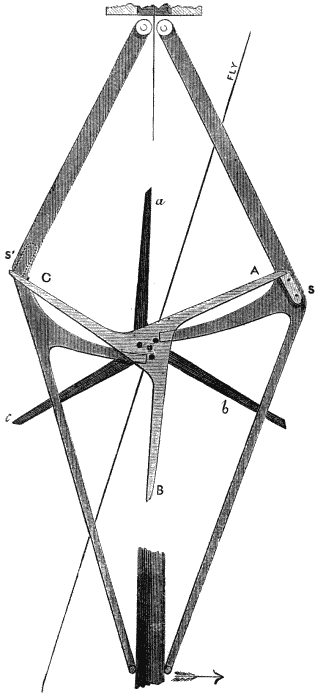
\includegraphics[height=0.9\textheight]{images/fig24.png}\index{Three-legged!gravity escapement}
\label{fig24}
\end{figure}
%-----File: 145.png------------------------------------------------
%-----Folio: 130---------------------------------------------------
equidistant arrangement is the natural one, and is generally
used, though not invariably. I need hardly say that a pair of
wheels of this kind are very different from a six-legged wheel
which would only move $30^\circ$ at each beat, while this moves
$6^\circ$, besides other differences.

In this case the distance of the pendulum top from the
scape-wheel centre evidently = diameter of scape-wheel. The
lifting pins should not be farther from the centre than a $36$th
of this, or the pallets have to be inconveniently light and
thin: the pins and arbor may be solid as a three-leaved
pinion. They should be so placed that the one which is
holding up a pallet and the one which is going to lift next
may be vertically over each other, the third being on a level
with the centre---\textit{i.e.}, they will stand on the radii which form
the acting faces of the teeth of one wheel, as you see \hyperlink{fig24}{here}.

This escapement is the best for large\index{Gravity escapements!best for large clocks} clocks, which must
have plenty of superfluous force to drive the hands in all
weathers (which superfluous force all reaches the pendulum
in clocks of the old kind, varying immensely); but the fly\index{Fly, striking!for gravity escapements}
must, on that account, be much larger in proportion
than in regulators, and care must be taken in planning
the clock to leave room for it. In the smallest turret clocks
I have always had the fly a foot long altogether and $1\frac14$in.\ wide,
and in large ones considerably more. When the fly
is very large, as at Westminster, the friction of a spring on
the arbor is not enough, and there must be a larger `roller'
or blank-wheel pinned on the arbor for the spring to act on.
At the same time it was very satisfactory to find that when
the men had once forgotten to screw up the spring after
doing something to the fly, the clock had never tripped in
the days which had elapsed; and I have tried the same
experiment elsewhere; but the four-legs will trip if the fly is
loose. The greater obliquity of the pallets, $30^\circ$ against $22\frac12^\circ$,
is the cause of this superiority of the three-legs; and this
obliquity may be increased still more if you like by altering
%-----File: 146.png----------------------------------------------
%-----Folio: 131-------------------------------------------------
the relative position of the two scapewheels. But I by no
means advise the omission of the fly, even then.

In very large clocks\label{large} the pallet tails are too thick to bend
for adjustment of the beat, and then eccentric beat pins are
used, which require no description. They are usually
made of brass, even in small clocks; but I think it would be
better to cover them with hard wood\index{Beat pins!ivory and wooden}\index{Wooden!beat pins}\markright{WOODEN BEAT-PINS.}. The finest clock of
this kind I have seen was a regulator with four-legged escapement
made by an amateur, Mr.~George Salt, of Saltaire;
and it had ivory beat pins, which certainly had less chatter
than brass ones. The pendulum weighed nearly $40$~lbs.,
and yet the clock weight was only $15$~lbs., with about $4$~ft.\ fall.
This shows that a gravity escapement really requires
very little more force than a dead one with as good a train
as possible, though practically I should always make the
weight abundant. One thing must be specially attended to,
as a distinction between these and dead escapements: the
beat pins must on no account be touched with oil or grease
of any kind, but left absolutely dry, whatever they are made
of; for the slightest adhesion to the pendulum is fatal; though
in dead escapements the fork should always have a drop of
oil, to keep it as close as possible without being tight. Moreover,
care should be taken to make one pallet begin to lift
simultaneously with the resting of the other, and neither
before nor after.

The best evidence of the performance\index{Gravity escapements!rate of some}\index{Rate!of some other gravity escapement clocks} of these escapements
is the annual report of the largest of them all at Westminster,
of which I shall have more to say afterwards.\footnote{And I have read in the \textit{English Mechanic} that one under the
charge of Professor Waldo, of Yale College Observatory, had gone for
several months on a rate of only $.47$~sec.\ a week.} My own have
often gone for months together without any difference from
Westminster for which I could venture to correct, or to
regulate the pendulum. I have never found on close inquiry
that the rate of the very best dead escapement regulators
%-----File: 147.png----------------------------------------------
%-----Folio: 132-------------------------------------------------
approached that of Westminster and several other public
clocks of this kind, of which I have occasionally had reports.
I have had accounts of some that had been altered from
other escapements to this, with the effect of reducing errors
of minutes to seconds. The last was from a gentleman
who said that his turret clock, made from this book by a
man who had never made one before, has a better rate
than any astronomical clock he had ever known.\index{Escapements, gravity!Beckett's|)}\label{gravend}

\section{CONSTRUCTION OF THE GOING PART OF CLOCKS.}\label{sec:GOING_PART.}\index{Clocks!going part of}\index{Going part of clocks}\markboth{GOING PART OF CLOCKS.}{GOING PART OF CLOCKS.}

Fig.~\ref{fig25} (p.~\pageref{fig25}) shows the arrangement of the going part of
a common regulator, or a house clock of superior character,
except that the pendulum in a clock of that kind ought to be
hung by a cock on the back of the case; but I have already
given a drawing showing that at p.~\pageref{fig09}; so I show another
mode of suspension here. In the common recoil escapement
clocks the pendulum only weighs a pound, or less, and is
hung from a cock merely screwed to the back plate of the
frame, which is a much weaker plan than this. $\mathrm{A}a$ is one of
the pallets on the arbor $a$ and $\mathrm{E}f$ the crutch and fork;
which generally embraces the pendulum, but sometimes goes
through it, especially when it is a wooden rod. The weight
is not hung by the single line, but by a double line going
through a pulley, sometimes in the weight itself, but more
frequently hung to it by a hook. This prevents the string
from untwisting, and enables you to do with a thinner string,
and it requires a barrel of twice the diameter which a single
string would, and that is worth something when the pivots
of the barrel are as large as they usually are, of which I have
spoken already at p.~\pageref{largepivots}. But it must be remembered that
every pulley in a machine, and especially every moveable
pulley, wastes power very sensibly by the friction and stiffness
of the rope, especially when the moving power is at the
slow end of the system of ropes. Theoretically it makes no
%-----File: 148.png----------------------------------------------
%-----Folio: 133-------------------------------------------------
difference whether a given weight with a given fall in a week
is hung by one rope without any pulleys or by half a dozen;
but practically you will find the weight has to be increased
in a very high ratio for every additional pulley you add.
You might soon reach a number at which no weight whatever
would do the required work, but would all be wasted in
overcoming the friction and stiffness of the ropes. This
remark is chiefly important with reference to turret clocks,
since not one architect in a hundred ever consults a clockmaker
before he plans either dial-holes or clock-room or
place for the weights to fall, and then people think it is the
clockmaker's fault if the clock does not perform as well as if
it had plenty of room for the weights to fall and other things
to act properly.

The barrel is fixed to its arbor, of which the back end is a
common pivot, but the front is carried through to the dial $\mathrm{K}$
and is squared for the key to take hold of it. The great
wheel $\mathrm{G}$ rides loose on the arbor between the barrel and a
collar shown just above $\mathrm{G}$ and it is connected with the
barrel by the ratchet and click, of which a front view and
description has been already given at page~\pageref{fig04}. (There are
in fact two ratchets $\mathrm{R}$ and $r$ in fig.~\ref{fig25}, but we need not
inquire into the functions of the second at present: it will
be explained at p.~\pageref{2ratchets}.) The great wheel $\mathrm{G}$ drives the
centre pinion $c$, which always turns in an hour, and its arbor
goes through to the dial and carries the minute hand in the
way I will describe presently. The centre wheel $\mathrm{C}$ drives
the second pinion $d$, on whose arbor is a wheel $\mathrm{D}$ which
drives the scapewheel $\mathrm{E}$ by its pinion $e$. In moderately good
clocks the pinions have all generally \index{Wheels, numbers of teeth}$8$ teeth or leaves, and
the wheels in that case have $96$, $64$, and $60$ teeth, if the
scapewheel turns in a minute as usual: in the best clocks
the pinions are occasionally as high as $16$; Mr.~Bloxam's
and Mr.~Salt's are the only ones I ever saw with higher
numbers. Of the scape-wheel, pallets, and pendulum, I
%-----File: 149.png-----------------------------------------------
%-----Folio: 134--------------------------------------------------
\begin{figure}[htbp]
\centering\index{Clocks!arrangement of common}\index{House clock, common}
\caption{\sc Common House Clock}
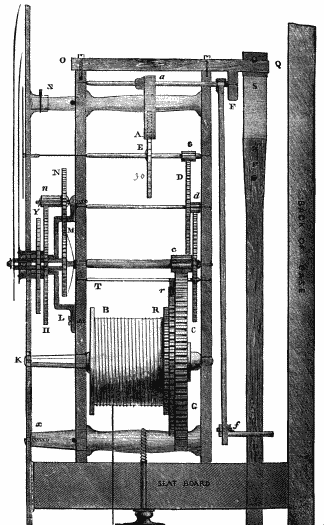
\includegraphics[height=525pt]{images/fig25.png}
\label{fig25}
\end{figure}\markright{COMMON HOUSE CLOCK.}
%-----File: 150.png-----------------------------------------------
%-----Folio: 135--------------------------------------------------
have said enough already. In the best clocks, and sometimes
in common ones, the scapewheel arbor comes through
the dial and carries a seconds hand.

Short clocks with half second pendulums are best made
with a scapewheel of the usual number of $30$ teeth, as
either a large and heavy wheel, or teeth very closely set, are
objectionable. In that case the scapewheel will of course
turn twice in a minute, and the product of the numbers of
the teeth of the centre and second wheels must $= 120 \times
8 \times 8$ if the pinions are of $8$, which is best satisfied by $96$
and $80$. In very inferior clocks the scapewheel pinion is
only $7$, and then $84$ and $80$ teeth will do. The American
clocks\index{American clocks}\index{Clocks!American} have lantern\index{Lantern pinions for clocks} pinions, in which $6$ pins are as good
as $8$ or $9$ common teeth, and therefore the centre and
second wheels need only have $72$ and $60$ teeth for a half-seconds
pendulum. It is not worth while to go on with
the calculation for $\frac23$~seconds pendulums or others, as the
principle of it is perfectly obvious.

\subsection[Dial work.]{Dial work.}\markboth{COMMON DIAL WORK AND SPRING.}{COMMON DIAL WORK AND SPRING.}\index{Dial work!of house clocks}---If the minute hand were fixed rigidly to the
centre arbor, the clock could never be altered; and therefore
the way in which it is fixed and yet alterable is this: there
is a wheel $\mathrm{M}$ (in fig.~\ref{fig25}) set on a hollow arbor or pipe which
fits easily on the centre arbor, and has its own end squared
for the hand to fit it. A small bent spring with a hole in the
middle fits on the centre arbor, and the hole rests against a
shoulder which is turned on the arbor just in front of the
clock frame; the ends of the spring press against the back
of the wheel $\mathrm{M}$ when it is pressed back, as it is after the
hand is put on, and it is kept there by a collar and a small
pin put through the end of the centre arbor.

And in this small matter there is room for a very common
mistake: the hand is kept steady by the friction of this
spring at one end and the collar at the other, and it will evidently
be much steadier for the same amount of pressure if
the spring fits the arbor tight, and so the friction is between
%-----File: 151.png-----------------------------------------------
%-----Folio: 136--------------------------------------------------
the ends of the spring and the back of the wheel, than if it
is loose on the arbor, simply on account of the difference of
leverage at which the friction acts when you turn the hand
with your own finger. In mere regulators without any striking
part, this does not matter, because there is nothing to
disturb the hand; but when the wheel $\mathrm{M}$, or the equal wheel
$\mathrm{N}$ which is driven by it, has to lift a lever every hour to discharge
the striking part, it matters a great deal, because a
great deal more friction is then required to hold it in its
place against the pressure of the lever; and yet it seems to
be the fashion in London to make the hole in the spring
round instead of \label{squaring}squaring it on to the arbor; which would
take about ten minutes to do. The consequence is that a
clock will sometimes take to losing unaccountably in this
way, which I only first discovered by seeing the minute
hand gradually lag behind the seconds hand; and that defect
can only be permanently cured by making the \label{strong_spring}spring very
much stiffer than it need be if it is put on properly, \textit{i.e.}\ with
a square instead of a round hole.

Over the minute-wheel $\mathrm{M}$ and its hollow arbor there is
fixed a thing called the \textit{bridge,} which is shown at $\mathrm{ML}$ (fig.~\ref{fig25}),
and has another pipe enclosing that of the wheel $\mathrm{M}$ but not
touching it; and the hour-wheel $\mathrm{H}$ with another hollow
arbor still larger rides upon the bridge pipe, and is driven by
a pinion $n$ of $1$-$12$th its own number of teeth, which is fixed
to the wheel $\mathrm{N}$ of the same number as $\mathrm{M}$\@. That wheel $\mathrm{N}$ is
generally set upon a stud or pin screwed into the front plate,
but is better with pivots in the frame and a cock. The hour
hand is set on the end of the hour-wheel socket either with
a small screw or pins. The thing marked $\mathrm{Y}$ in front of
the hour-wheel has nothing to do with the going part of
the clock, but is the \textit{snail} which regulates the number of
hours struck by the striking part, as will be explained
therewith.

The hour hand in astronomical\index{Clocks!astronomical} clocks generally has a
%-----File: 152.png----------------------------------------------
%-----Folio: 137-------------------------------------------------
small circle to itself in the lower half of the dial, to prevent
its hiding the seconds hand in the upper half, which it is
important that an observer should always be able to see.
Besides it moves with much less friction when so placed, as
it then turns on a thin stud fixed on the front plate of the
clock, instead of a very wide socket. It may either be
driven by an intermediate wheel and pinion from the centre
arbor, in order to make it go the right way round, or directly
by the great wheel, which involves less friction and no inconvenience
except the perfectly insignificant one of having
to move the hour hand separately from the minute hand
when you want to alter the clock much, which cannot happen
once a year in any good clock.

\subsection[Dial.]{Dial.}\markboth{REGULATOR DIAL WORK.}{REGULATOR DIAL WORK.}\label{subsec:Dial_work.}\index{Astronomical clocks!dial work of}\index{Dial work!of house clocks}---Two different ways of fixing a dial are shown in
fig.~\ref{fig25}, and both of them different from the common one, in
which four separate pillars are screwed permanently into the
dial and the other ends go through the front clock plate and
are pinned behind it, the main pillars of the clock itself
being only long enough to connect the two plates, and
having nothing to do with the dial. Either of the two plans
in the figure seems to me to be better than this, though it is a
matter of very little consequence. The dials of the best
clocks are made of brass plates polished and silvered: the
common ones are of sheet iron: the American and Dutch of
wood. The hands\index{Hands of clocks and watches!the best colours for} are always of black steel in regulators\label{reg},
but in common clocks they are of brass gilt, which is a very
bad colour on a white face, though very good on a black
face. The same remark applies to watch faces. I never
could understand how such an absurd thing as gold hands
on white faces---and still worse on gilt faces---came into
existence, especially as gold hands of that small size have
not even the vulgar merit of being dearer than steel
ones.

\subsection[Winding keys]{Winding keys}\markboth{WINDING KEYS SHOULD BE LONG.}{WINDING KEYS SHOULD BE LONG.}\ \label{subsec:Winding_keys}\index{Key!for clocks}\index{Keys, winding}\index{Winding keys!for clocks}are generally made too \index{Winding keys!should be long}short in the stalk
or leverage, which makes the clock harder to wind and tends
%-----File: 153.png----------------------------------------------
%-----Folio: 138-------------------------------------------------
to strain the arbor besides, as you may see from considering
that if the stalk was very short indeed, any force applied to
it would be chiefly consumed in trying to bend the arbor.
As there is absolutely no advantage in a short key, this is
one of the many instances of doing wrong for the pleasure of
it, when it would be quite as easy to do right and the effect
much more pleasant. All my seconds pendulum clock keys
are from $3$ to $5$~inches long, according to the weights.
The French spring clocks without fusees, in which the winding
is very hard towards the end, have keys like a very
large watch key or a piano-tuner, to prevent the strain
upon the arbor. But this makes the winding a much longer
operation and a very unpleasant one, as you have to stop
at every half turn. Sometimes such keys are given with
small English fusee clocks, for which there is no excuse.
You should take care that the wood or ivory on the handle
of a key is quite loose, or it increases the resistance materially
in winding.

\subsection[Year clocks.]{Year clocks.}\markboth{YEAR CLOCKS.}{YEAR CLOCKS.}\label{subsec:Year_clocks.}\index{Clocks!year}\index{Year clocks}---Clocks without striking parts are sometimes
made to go a month, and occasionally even a year.
For a month they only require one more wheel and pinion
with a multiplier of $4$, between the centre and great wheels.
Year clocks require $3$ wheels below the centre, and the
pinions ought to be of $10$, $10$ and $12$ at least, on account of
the great weight required, which will have to be still greater
if the pinions are of low numbers. Assuming the clock to
go $380$~days, and the barrel to have $16$ turns as usual, the
product of the $3$ wheels must $= \frac{380.24.12.10.10}{16}$, for which
$100$, $90$, and $76$ will be the best numbers. This is far better
than trying to do it with only two wheels of $192$ and $190$
(the lowest possible numbers), and pinions of $8$, in which
the friction will be very much greater. The best way is to
have two barrels and great wheels acting on one long pinion
of $12$, with the weight hung by the same string from both
%-----File: 154.png---------------------------------------------
%-----Folio: 139------------------------------------------------
barrels by a pulley which only turns while you are winding
up; and there must be a winding stop to each barrel.

\subsection[Clock cases]{Clock cases}\markboth{CLOCK CASES.}{CLOCK CASES.}\ \label{subsec:Clock_cases}\index{Clock-cases}are necessarily connected with the construction
of the clock. The old tall case with a base as big as
the top, standing on the floor instead of screwed to the wall,
is sufficiently \correction{explored}\label{correction2} %**Transcriber's note: The original reads "exploded".
to require no more to be said against
it. The case need be no longer than is required for the
pendulum, as the weights can have $3$ lines, or smaller barrels,
or larger great wheels, of which the second is the worst. The
weights themselves of course have to be half as heavy again
as with the fall one half longer. The best case for a superior
clock is one of which the front and sides take off together.
There need be no door to the face, but only small brass or
white metal shutters over winding holes in the plate glass
front, which enables you to lock up the clock completely and
leave anybody to wind it up. Ornamental case making I
have nothing to do with, and it is not much of an exaggeration
to say that the value of the inside of a clock generally
varies inversely as the decoration of the outside.

\subsection[Moon dials.]{Moon dials.}\markboth{MOON DIALS.}{MOON DIALS.}\label{subsec:Moon_dials.}\index{Dials!moon}\index{Lunar clocks}\index{Moon dials}---There is an old calculation that if a pinion
of $6$ is put on the hour arbor of a clock---\textit{i.e.}\ the centre
one---and drives a wheel of $91$ with a pinion of $9$ on its
arbor driving another wheel of $91$ with a pinion of $37$ driving
a wheel of $171$, that last wheel will turn in $29$d.~$12$h.~$44$m, $3.4$s., which is only about half a second more than an
average lunation. A pinion of $6$ does very well for a driving
one, though it is much too low a number for a driven pinion,
except of the fly of the striking part. But if the centre
pinion is $12$ and the great wheel $182$, those two will do for
the first pair of such a lunar train. In that case, as the
arbor of the great wheel must turn for winding, it would be
necessary to fix the $37$ wheel on the back of the great wheel,
and let that drive either the $91$ or the $171$ as may be convenient;
for the order in which wheels and pinions are
arranged is immaterial as to the velocity-ratio between
%-----File: 155.png--------------------------------------------
%-----Folio: 140-----------------------------------------------
the first and the last. The common moon dials of old-fashioned
clocks are only driven by a single tooth on the
hour arbor driving a wheel of $59$ teeth by jumps twice a
day, leaving an error of $44$~m.\ in a month, to be set right by
hand every now and then.

A simpler moon train, quite exact enough for this purpose
may be made by a pinion of $15$ on a $24$-hour wheel of the
clock driving a $98$ wheel with a pinion of $25$ driving a wheel
of $113$, which will turn in $708.736$~hours, which is only an
excess of $7$~seconds over one lunation of $708.73415$~h., or $3$
minutes in $2$ years, which would be quite imperceptible in
any dial. But nobody seems to remember that no flat moon
dial can possibly imitate more than one phase of the moon,
either just half-moon, or else the narrowest possible crescent;
for the \textit{terminator}, or boundary of light and shade on the
moon, is always a semi-ellipse, varying continually from
the nearest visible approach to a semicircle down to a
straight line and then back again. The only way in which
real phases can be shown is by a globe half white or gilt and
the other half black, turning on an axis in the plane of the
dial in a hole just fitting the globe. And that only will look
like the moon when seen right in front and from a considerable
distance, as the moon is. Practically a vertical
axis will do, though I need not say that the diameter which
joins the `horns' of the terminator is seldom quite upright,
and sometimes leans a good deal either way (see my `Astronomy,'
p.~140 of 7th ed.). The axis must be turned by
a bevelled wheel, of which half will come through the dial---or
above, if you want to hide it. But all such contrivances
are mere playthings, and show the moon's phases much less
distinctly than an almanac.

\subsection[Day of the month dials]{Day of the month dials}\markboth{DAY OF THE MONTH DIALS.}{DAY OF THE MONTH DIALS.}\label{subsec:Day_of_the_month_dials}\index{Clocks!day of the month}\index{Day of the month dials}\ have to be dealt with rather
differently, because the move must take place only once in
the $24$~hours, at some time in the night. Consequently the
wheel which carries either a small dial with figures showing
%-----File: 156.png---------------------------------------------
%-----Folio: 141------------------------------------------------
through a hole, or a hand pointing to figures, must have
ratchet teeth driven by a lever or click or tooth moved once
a day. There must also be a slight spring or `jumper' somewhere
on the ratchet teeth to keep them exactly in the proper
place for the click to catch next time. In the old-fashioned
clocks the month wheel simply had $31$ teeth, and you had to
move it on by hand in February, April, June, September, and
November.

\begin{figure}[hbtp]
\centering
\hypertarget{fig26}{\caption{\sc Day of the Month Dials}}
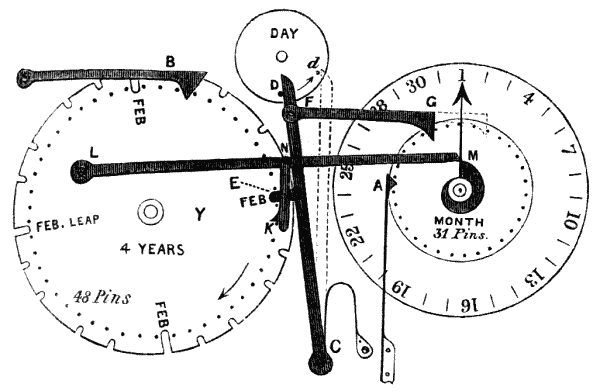
\includegraphics[width=\textwidth]{images/fig26.png}
\label{fig26}
\end{figure}

I doubt if such clocks, however completely automatic, are
really of much use, for this reason if for no other, that the figures
of the day of the month are always too small to be seen at such
a distance as clocks usually are when you are writing and
want the date. Large cards, changed every day, are infinitely
more used. Nevertheless, as the machinery is, or may
be, much simpler than you would suppose beforehand, I may
as well indicate the nature of it, on what seems to me the
simplest of the various ways of doing it. But for the present
foolish arrangement of months, which the world seems impotent
to set aside, we should only want six months of $30$
%-----File: 157.png---------------------------------------------
%-----Folio: 142------------------------------------------------
days, and six of $31$ in leap years, and in other years seven
and five. But, as things are, we have four kinds of month
to provide for. We must clearly have one wheel $\mathrm{M}$ with $31$
teeth, carrying a hand pointing to a month dial; for that is
much easier to see than numbers peeping through a hole, and
it is enough to print every third number, except at last $28$--$30$--$1$.
Then we want some contrivance to push on two
teeth in April, June, September, and November, three in
February in leap year, and four in other years.

Let there be a $24$~hour wheel \textsc{Day}, which, by the
pin at $\mathrm{D}$ moving on to $d$, will move the long lever $\mathrm{CEFD}$ so
much to the right as will carry the horizontal click $\mathrm{FG}$ over
the space of $4$ teeth or pins of the month wheel, \textit{i.e.}\ will
drive that wheel $4$~days forward. That provides for common
Februaries. Then if the lever $\mathrm{CD}$ is stopped from going
more than the space of one tooth of $\mathrm{M}$ back again at the end
of the long months, as of other days, they also are provided
for. It must fall back the space of two teeth at the common
short months, and three teeth at the end of leaping Februaries.
Several ways have been invented for doing this. The simplest
is to have a four-year wheel, or disc $\mathrm{Y}$, with $4$ deep February
notches in it at quadrants, into which a long tooth $\mathrm{E}$, on the
lever $\mathrm{CED}$, can drop, and short notches for the $30$-day
months, and none for the long months, but the outside of the
wheel $\mathrm{Y}$ is the space of one tooth off the tooth $\mathrm{E}$ generally.

But we have to consider how the year wheel is to be
moved at the end of every month, as it must be, and so as
not to be held fast by the tooth $\mathrm{E}$ in any notch. I think the
best way is to do it by another lever $\mathrm{LNM}$ on a stud in the
clock frame at $\mathrm{L}$, and a gathering click $\mathrm{NK}$, which takes
hold of one of the $48$ pins in $\mathrm{Y}$ when that lever is lifted, and
carries $\mathrm{Y}$ one step or month-space forward when the lever is
dropped by the snail $\mathrm{M}$ just before the last move of the month
is finished, or as the hand comes up to $1$. This divides the
work of moving the two wheels and levers more uniformly
than any other plan, besides making sure of the tooth $\mathrm{E}$
%-----File: 158.png--------------------------------------------
%-----Folio: 143-----------------------------------------------
being out of a notch before the year wheel wants to move:
not that it would signify on this plan if it were not, for then
the lever $\mathrm{LNM}$ would only wait to drop. Each of the wheels
wants a safety click or juniper, $\mathrm{A}$, $\mathrm{B}$, of the usual kind for
such motions. I only put pins instead of ratchet teeth to $\mathrm{M}$,
because the click $\mathrm{FG}$ will be safer not to slip out.

The work might be simplified a little and the lifts made
less, and the year wheel need only be a quarter of the size,
if you will be content to move the month hand at the end of
February by hand. A week dial is quite superfluous, and so
I have not crowded the picture with one. It only wants a
seven-star wheel by the side of the day wheel, one ray of
the star being moved by the pin $\mathrm{D}$ after it has come to $d$ and
done its monthly work. It is desirable to distribute the
work as much as possible. The month dial ought to be at
least twice as large as in \hyperlink{fig26}{this drawing}, to be seen easily.

In any clock which has all this extra work to do, special
care must be taken that the `motion' wheels (or dial work)
are held on the centre arbor by a squared spring, and a pretty
strong one (see p.~\pageref{strong_spring}), or it is sure to slip and gradually
drag, though the clock may be going right.

Several\markboth{DIALS WITHOUT HANDS.}{DIALS WITHOUT HANDS.} persons have taken patents for clocks and watches
showing the time by figures appearing through a hole in the
dial instead of by hands.\index{Chronoscopic dials} Not that there is anything new in
that, except as to the machinery for doing of it. Days of
the month were generally so done 100 years ago at least;
and my old regulator by Holmes\index{Holmes, an old clockmaker}, already mentioned at p.~\pageref{holmes},
shows the hours in that way. I do not profess to judge of
public taste, but it seems to me that all such inventions proceed
on the fundamental mistake of supposing that we \textit{read}
the figures of a dial. We do nothing of the kind, but judge
at once from the mere position of the hands and the well-known
marks for the hours and minutes. In fact dials are
better and clearer with no numbers at all, but merely $12$
large spots for the hours and five-minutes, and $48$ small
ones for the other minutes, as I have often convinced people
%-----File: 159.png--------------------------------------------
%-----Folio: 144-----------------------------------------------
by asking them if they want such a dial as they see in
several of my clocks. They always answer `Yes;' and
then are much surprised to find no figures, but only
the $12$ strong marks and $48$ small ones. And the
hands upon a dial, whether large or small, are more
conspicuous than any figures which can be conveniently
made to appear through a hole, especially if the hands are
of the proper colour\index{Hands of clocks and watches!the best colours for}---\textit{i.e.}\ black on a white or gilt dial or
gilt on a black one.

Moreover, there is another objection to those `chronoscopic'\index{Chronoscopic dials}\index{Dials!chronoscopic}\label{chronoscopic}
dials: the figure-discs must be driven discontinuously,
or by jerks at the end-of certain periods; and if that is done
directly by the watch, as in Barlow's patent of 1866, the
strain on the wheels is so much greater at the short time of
action, and especially when the units and tens of minutes and
the hour all have to be changed at once, that it is impossible
for such a watch to go well. Besides the mere work of
moving the $3$ discs, all from the $5$-minute wheel of the train
with different intermediate wheels, there are jumper springs
to be moved too. Whether such watches have been ever been
made I do not know; I have only read the specification.

It was patented in 1869 for clocks in a more practicable
form by \index{Siddons and Meese's clocks}Siddons and Meese, who brought me one to examine.
They have $3$ cylinders, $\mathrm{A~B~C}$, near together; $\mathrm{A}$
with the ten digits 0~1\dots\dots~9 on its face for units of
minutes, $\mathrm{B}$ with blank~1~2~3~4~5 (blank being better than $0$
there) twice over for the tens of minutes (making $12$ spaces),
and $\mathrm{C}$ with 1 up to 12 for the hours. An $8$-minute wheel
in the clock has $8$ pins in it, which are always lifting a
weighted lever, except at the moment when it drops from
one pin to another. The lever has a pall\footnote{If this word has any etymology it clearly should be spelt \textit{pall},
not from the \textit{pallium} of an archbishop or a corpse, but from $\pi\alpha\lambda\lambda\omega$, to
strike, the origin of pallet. `Paul' or `pawl' are mere nonsense, of
the same order as the vulgar conversion of the expressive Yankee word \textit{bunkum}, for bluster,
into \textit{buncombe}, for no other reason than because
newspaper writers know there is a noble family of Duncombe, or the
auctioneers' conversion of the site of a house into scite, which only
shows themselves to be insciti.} or click which
%-----File: 160.png--------------------------------------------
%-----Folio: 145-----------------------------------------------
\label{folio_145}first slips over and then brings down in falling one of $10$
ratchet teeth on the side of $\mathrm{A}$, and so changes it from one
figure to another. Whenever $\mathrm{A}$ changes from 9 to 0 it also
moves on $\mathrm{B}$ one figure by the usual contrivance of numbering
machines for railway tickets, bank-notes, and pages of
ledgers; and when $\mathrm{BA}$ changes from 5~9 to blank~0, $\mathrm{B}$ in
like manner changes $\mathrm{C}$ one figure, $\mathrm{B}$ having $2$ levers on its
side corresponding to the two blanks. There are other
details of minor importance in Siddons and Meese's clocks,
for which the patent has been transferred to Gillett and
Bland, of the Steam Clock Factory at Croydon.

As descriptions of the numbering machine are not
easy to find, I had better give one, at least sufficient to
illustrate its principle. Take first the simple case of
only two wheels or cylinders set near together on the
same axis, but loose, with the $10$ digits engraved on their
faces, one $\mathrm{A}$ for units and the other $\mathrm{B}$ for tens. A
carries on its side a small bent lever which generally
hangs loose, but at one place in the revolution, where $\mathrm{A}$ is
changing from 9 to 0, the lever has its tail caught by a fixed
obstacle, and for that moment the other end of the lever
cannot yield, but travels with its wheel. $\mathrm{B}$ has $10$ pins on
its side, and whenever the lever of $\mathrm{A}$ is in that condition it
catches one of those pins and so drives on $\mathrm{B}$ one step, or
changes it one figure. Then for the hundreds, $\mathrm{B}$ has a
similar lever on its other side which changes a wheel $\mathrm{C}$ in
like manner, and so on for as many figures as are wanted.
In clocks the change of the $10$-minute wheel has to be made
after 5 so as to show 0 or a blank next, instead of after 9 as
in numbering machines.

\subsection[Equation of time clocks.]{Equation of time clocks.}\markboth{EQUATION OF TIME CLOCKS.}{EQUATION OF TIME CLOCKS.}\label{subsec:Equation_of_time_clocks.}\index{Clocks!equation of time}\index{Equation of time clocks}---A still more obsolete contrivance,
%-----File: 161.png--------------------------------------------
%-----Folio: 146-----------------------------------------------
but worth recording for the principle of its
machinery, was that for making the hands of a clock show
solar instead of mean time, at least in a rude and approximate
way, which I suppose was used in the French public
clocks which did so up
to the year 1826. $\mathrm{A}a$ in
\hyperlink{fig27}{this figure} is a bevelled\label{bev}
wheel on the centre wheel
arbor, which in this case
is made to turn the
wrong way round, and
another equal bevelled
wheel $\mathrm{B}b$ rides upon it,
with a hollow spindle $bc$
to which the minute-hand
is fixed. Between these
two is another small
bevelled wheel $\mathrm{D}$ of any
size, which would merely
reverse the motion, if it
was set on a fixed spindle
or arbor. But it is not,
for it rides on the end of
a bar or lever $\mathrm{DE}$, which
itself turns upon the centre
arbor and has its end $\mathrm{D}$
beyond the wheel resting
on a plate of the odd
shape shown at $\mathrm{Q}q$, which
is fixed to the face of a
wheel which turns in a
year. Now if the lever $\mathrm{DE}$, or the centre of the small wheel,
is moved at any time in the same direction as the hand is
going, it will evidently push it forward just twice as much as
the lever itself is moved, and \textit{vice vers\^a.} If then the equation
\begin{figure}[htbp]
\centering
\hypertarget{fig27}{\caption{\sc Equation of Time Clock}}
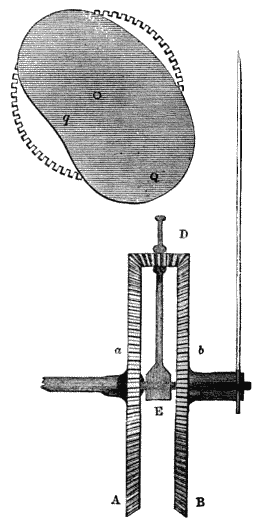
\includegraphics[height=0.7\textheight]{images/fig27.png}
\label{fig27}
\end{figure}
%-----File: 162.png--------------------------------------------
%-----Folio: 147-----------------------------------------------
plate $\mathrm{Q}q$ is on the right side of the clock-frame, the hand will
go ahead of its mean motion whenever $\mathrm{D}$ drops below the
mean radius of the plate from $\mathrm{O}$ the centre of the year wheel
and will fall behind mean time when the protuberant parts
of the plate are uppermost. The plate then may be so
shaped as to make the advance and retardation of the hand
agree with the `sun before clock' and `sun after clock' of
the equation of time.

There are two other ways of giving a secondary motion
of this kind; one, by substituting a common small wheel or
pinion for the middle bevelled wheel, and putting it between
$\mathrm{A}a$ made as a common wheel, and $\mathrm{B}b$ made as an \textit{internal}
wheel, \textit{i.e.}\ with teeth inside its rim; but in that case you
must remember that $\mathrm{A}$ and $\mathrm{B}$ will have different velocities,
and therefore $\mathrm{A}$ must turn in less than the hour. The other
method requires neither bevelled nor internal wheels, and is
on the same principle as the one I shall describe more fully
under \textit{train remontoires.}

Clocks for showing other celestial motions are mere
curiosities, and are always getting out of order from their
complication; so I shall not waste time in describing them,
but go on to something more practical.

\section{MAINTAINING POWERS OR GOING BARRELS.}\markboth{MAINTAINING POWERS.}{MAINTAINING POWERS.}\label{sec:MAINTAINING_POWERS_OR_GOING_BARRELS.}\index{Barrels, going}\index{Maintaining powers of clocks or going barrels}

Winding up a clock evidently takes the action of the
weight off the great wheel, and so the clock movement stops
for the time, though the pendulum goes on swinging. This
of course will not do in a clock of any accuracy, whether a
large or a small one, and as the same methods of keeping
the clock going (or some of them) are applied to both, I
shall describe them all together here, except one.

The oldest of them all is \index{Huyghens!endless chain}\textit{Huyghens's endless chain.}\index{Maintaining powers of clocks or going barrels!endless chain}\label{endless} In
fig.~\ref{fig28} $\mathrm{P}$ in the `going wheel' is a pulley fixed to the
great wheel of the going part, and having short spikes set in
%-----File: 163.png-----------------------------------------------
%-----Folio: 148-----------------------------------------------------
it, or roughened in some other way so as to prevent a rope
or a chain hung over it  from slipping.     A similar pulley
rides on another arbor $p$, which may be the arbor of the
great wheel of the striking part, if the clock has one, and
attached by a  ratchet and click to that wheel, or to the
clock-frame if there is no  striking part.    The weights are
hung as you see, the
little   weight   being
only big  enough to
keep  the   string   in
the pulleys\index{Pulleys}; but the
string   or   chain   is
much longer, or one
at least of the weights
is always lower down
than   I   have   been
obliged   to   draw it
\hyperlink{fig28}{here}.    If you pull $b$,
the left hand of all
the   strings,   down,
the   ratchet   pulley
moves under the
click, and the great
weight is pulled up
by $c$, without taking
its pressure off the
going wheel  at all.
This plan was generally
used in the old $30$~hour clocks, but went out with them,
as the action of a chain or even a rope hung in that way is
rough  and uneven;   and moreover the pulleys must be of
only half the usual diameter for the same time of going.

\begin{figure}[ht!bp]
\centering
\hypertarget{fig28}{\caption{\sc Endless Chain}}
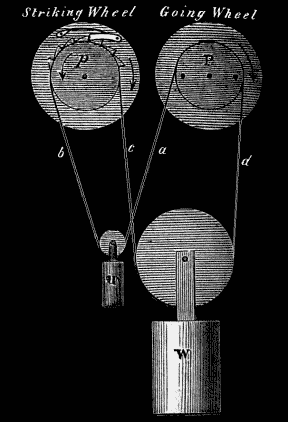
\includegraphics[width=288pt]{images/fig28.png}
\label{fig28}
\end{figure}

\subsection[Harrison's going barrel]{Harrison's going barrel}\markboth{SPRING GOING BARREL.}{SPRING GOING BARREL.}\label{subsec:Harrison's_going_barrel}\index{Harrison!going barrel}\index{Maintaining powers of clocks or going barrels!Harrison's} is the maintaining power used
in all regulators now. The larger \label{2ratchets}ratchet wheel\index{Ratchet wheels} $r$ is the
one designated by the same letter in fig.~\ref{fig25} (p.~\pageref{fig25}); and
%-----File: 164.png----------------------------------------
%-----Folio: 149-------------------------------------------
the click $\mathrm{R}$ is fixed to that wheel, which is connected with
the great wheel by a spring $\mathrm{SS}'$. While the clock is going the
weight acts on the great wheel $\mathrm{G}$ through the spring; but as
soon as you take off the weight by winding, the click $\mathrm{T}r$,
whose pivots are set in the frame, prevents the great ratchet
from falling back, and so the spring still drives the great
wheel during the time the clock takes to wind, especially as
it need only just keep the escapement going, for the pendulum
will take care of itself for that short time. The drop of
the great click over the teeth of its ratchet may be heard
\begin{figure}[ht!bp]
\centering
\hypertarget{fig29}{\caption{\sc Spring-going Barrel}}
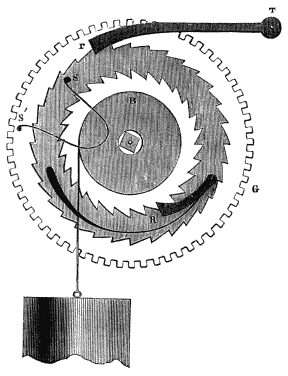
\includegraphics[width=288pt]{images/fig29.png}
\label{fig29}
\end{figure}
%-----File: 165.png-----------------------------------------------
%-----Folio: 150--------------------------------------------------
every $10$~minutes or so while the clock is going. Watches
have the same apparatus, with a spring click.

\subsection[Bolt and shutter.]{Bolt and shutter.}\markboth{OTHER MAINTAINING POWERS.}{OTHER MAINTAINING POWERS.}\label{subsec:Bolt_and_shutter.}\index{Bolt and shutter}\index{Maintaining powers of clocks or going barrels!bolt and shutter}---Another contrivance, which is now
used only in large clocks, is an arbor with a weighted lever
at one end of it, with a click in the form of a spring bolt on
another lever; when the weighted arm is lifted up the click
`takes into' the teeth of some one of the train wheels, and the
weight then keeps the clock going till it works itself out of
gear in a few minutes and drops. The weighted lever is
outside the clock and is made with a cap or shutter which
shuts over the key-hole when it is down, to make sure of
your lifting it before you begin winding. With the usual
ingenuity for doing things wrong, this click is very often
made not as a sliding bolt, but with a hinge, so that there is
one position of the lever in which it jams against the teeth
and stops the clock for good, unless the winding man finds
it out and releases it, which he probably will not. Sometimes
too the click sticks and sometimes it slips, even if made
rightly. There is another defect besides in the common
bolt and shutter, viz.\ that it may work itself down and rest
upon the winder or key before the winding is done if the
man is slow about it, and then it does no good and the clock
stops for the time.

\subsection[Improved bolt and shutter.]{Improved bolt and shutter.}\markboth{SIR E. BECKETT'S BOLT AND SHUTTER.}{SIR E. BECKETT'S BOLT AND SHUTTER.}\label{subsec:Improved_bolt_and_shutter.}\index{Bolt and shutter!Sir E.~Beckett's improved}\index{Maintaining powers of clocks or going barrels!bold and shutter!Beckett's improved}---To prevent these evils,
and to simplify the construction, I\index{Beckett, Sir E.!bolt and shutter} introduced the plan of
substituting for the `bolt' a segment $\mathrm{D}$, in fig.~\ref{fig37}, p.~\pageref{fig37},
of a small wheel suited to the teeth of the great wheel, and
making the arbor $\mathrm{C}$, which carries that and the shutter $\mathrm{M}$,
to pump in and out of gear, and the shutter not covering the
key-hole, but made as a circular arc to the centre $\mathrm{C}$, which
all but touches the winder when it is on. The winder has a
ring, shown by the circle at $\mathrm{M}$, fixed round its end, which
prevents it from being put on until you have lifted the
shutter, and put it into gear with the great wheel, to hold
it up. As you go on winding, the clock goes on and the
%-----File: 166.png-----------------------------------------------
%-----Folio: 151--------------------------------------------------
shutter descends, now behind the ring, which secures your
pulling it out of gear again when you take off the winder,
and yet it will keep in action full $10$~minutes if left to work
itself out. This plan is now generally used in superior
large clocks. The weighted arm should be long, so as not
to require a heavy weight to be lifted.

I shall describe hereafter another totally different plan
for keeping a very large clock going when the winding takes
a long time; but as the spring \label{smallmaintain}going barrel does very well
for small clocks, and the improved bolt and shutter for any
but a clock of quite unusual size, I shall postpone that
description till we come to the Westminster clock. For the
same reason I need not repeat the description of Sir G.~Airy's\index{Airy, Sir G.~B.!maintaining power}
going barrel, which was applied to the Exchange clock, but
is so expensive that it is certain never to be used again. A
full description of it was given by him in vol.~7 of the Cambridge
Phil.~Trans. The object of it was not only to keep
the power always on the clock, but exactly the same power;
for the power of the spring falls below that of the weight,
and that of the bolt and shutter doubles it just at the times
of putting it on and taking it off; but that is of no consequence,
except in a revolving pendulum clock, for which his
apparatus was invented; he afterwards simplified the construction,
but it is still an expensive one, and the thing can
be done at a tenth of the cost by the Westminster method
without either loss or duplication of force.

There is another maintaining power\index{Sun and@`Sun and planet' maintaining power}\markboth{`SUN AND PLANET' MAINTAINING POWER.}{`SUN AND PLANET' MAINTAINING POWER.} which has a tempting
and scientific look, but is not so good as it looks. A rim
at the back of the great wheel, $\mathrm{M}$ (fig.~\ref{fig29}), has internal
teeth at A---troublesome things to make---and in them works
a wheel $\mathrm{ABP}$ on a stud $\mathrm{B}$ in the end of the barrel, and also
in a pinion $\mathrm{C}$ fixed on the arbor which runs loose through
the barrel ends. When you wind up you apply some force $\mathrm{P}$
to the intermediate wheel, and the same pressure $\mathrm{P}$ is communicated
to the great wheel because $\mathrm{BP = BA}$, $\mathrm{P}$ being
%-----File: 167.png-----------------------------------------------
%-----Folio: 152--------------------------------------------------
\begin{figure}[htbp]
\centering\index{Maintaining powers of clocks or going barrels!sun and planet@`sun and planet' power}\index{Sun and@`Sun and planet' maintaining power}
\setlength{\unitlength}{0.028\textwidth}%needs to be this large for lines in diamond to be long enough for LaTeX.  Smaller \path available if epic, eepicemu packages loaded.
\caption{\sc Sun-and-planet Power}
\begin{picture}(30,28)(-13,-15)
%diamond in centre
\put(0,1){\line(-1,-1){1}}
\put(-1,0){\line(1,-1){1}}
\put(0,-1){\line(1,1){1}}
\put(1,0){\line(-1,1){1}}
%Circle centre (0,0) radius 3
\qbezier(3,0)(3,1.242641)(2.121320,2.121320)
\qbezier(-3,0)(-3,1.242641)(-2.121320,2.121320)
\qbezier(3,0)(3,-1.242641)(2.121320,-2.121320)
\qbezier(-3,0)(-3,-1.242641)(-2.121320,-2.121320)
\qbezier(2.121320,2.121320)(1.242641,3)(0,3)
\qbezier(-2.121320,2.121320)(-1.242641,3)(0,3)
\qbezier(2.121320,-2.121320)(1.242641,-3)(0,-3)
\qbezier(-2.121320,-2.121320)(-1.242641,-3)(0,-3)
%Circle centre (0,0) radius 12
\qbezier(12,0)(12,4.970564)(8.485280,8.485280)
\qbezier(-12,0)(-12,4.970564)(-8.485280,8.485280)
\qbezier(12,0)(12,-4.970564)(8.485280,-8.485280)
\qbezier(-12,0)(-12,-4.970564)(-8.485280,-8.485280)
\qbezier(8.485280,8.485280)(4.970564,12)(0,12)
\qbezier(-8.485280,8.485280)(-4.970564,12)(0,12)
\qbezier(8.485280,-8.485280)(4.970564,-12)(0,-12)
\qbezier(-8.485280,-8.485280)(-4.970564,-12)(0,-12)
%Circle centre (0,0) radius 12.5
\qbezier(12.5,0)(12.5,5.177670)(8.838835,8.838835)
\qbezier(-12.5,0)(-12.5,5.177670)(-8.838835,8.838835)
\qbezier(12.5,0)(12.5,-5.177670)(8.838835,-8.838835)
\qbezier(-12.5,0)(-12.5,-5.177670)(-8.838835,-8.838835)
\qbezier(8.838835,8.838835)(5.177670,12.5)(0,12.5)
\qbezier(-8.838835,8.838835)(-5.177670,12.5)(0,12.5)
\qbezier(8.838835,-8.838835)(5.177670,-12.5)(0,-12.5)
\qbezier(-8.838835,-8.838835)(-5.177670,-12.5)(0,-12.5)
%Circles centre (-7.5,0) radii 0.5 and 4.5
\put(-7.5,0){\circle{1}}
\qbezier(-3,0)(-3,1.863961)(-4.318020,3.181981)
\qbezier(-12,0)(-12,1.863961)(-10.681981,3.181981)
\qbezier(-3,0)(-3,-1.863961)(-4.318020,-3.181981)
\qbezier(-12,0)(-12,-1.863961)(-10.681981,-3.181981)
\qbezier(-4.318020,3.181981)(-5.636039,4.5)(-7.5,4.5)
\qbezier(-10.681981,3.181981)(-9.363961,4.5)(-7.5,4.5)
\qbezier(-4.318020,-3.181981)(-5.636039,-4.5)(-7.5,-4.5)
\qbezier(-10.681981,-3.181981)(-9.363961,-4.5)(-7.5,-4.5)
%Circles centre (15.5,0) radii 1 and 3
\put(15.5,0){\circle{2}}
\qbezier(18.5,0)(18.5,1.242641)(17.621320,2.121320)
\qbezier(12.5,0)(12.5,1.242641)(13.37868,2.121320)
\qbezier(18.5,0)(18.5,-1.242641)(17.621320,-2.121320)
\qbezier(12.5,0)(12.5,-1.242641)(13.37868,-2.121320)
\qbezier(17.621320,2.121320)(16.742641,3)(15.5,3)
\qbezier(13.37868,2.121320)(14.257359,3)(15.5,3)
\qbezier(17.621320,-2.121320)(16.742641,-3)(15.5,-3)
\qbezier(13.37868,-2.121320)(14.257359,-3)(15.5,-3)
%Horizontal lines
\put(1,0){\line(1,0){2}}
\put(-12,0){\line(1,0){4}}
\put(-7,0){\line(1,0){6}}
\put(12,0){\line(1,0){2.5}}
\multiput(3,0)(1,0){9}{\line(1,0){0.5}}%dotted line
%Vertical lines and arrows
\put(-12,0){\vector(0,-1){15}}
\put(-3,0){\vector(0,1){6}}
\put(0,1){\line(0,1){2.5}}
%Labels
\put(0,3.7){\makebox(0,0)[b]{C}}
\put(15.5,3.5){\makebox(0,0)[b]{H}}
\put(-3,6.2){\makebox(0,0)[b]{P}}
\put(-7.5,0.7){\makebox(0,0)[b]{B}}
\put(-11.8,0.2){\makebox(0,0)[bl]{A}}
\put(-9,9){\makebox(0,0)[br]{M}}
\put(-11.8,-15){\makebox(0,0)[bl]{W}}
\end{picture}
\label{fig30}
\end{figure}
whatever is necessary to lift the weight. Let $\mathrm{W}$ be the
effective weight at $\mathrm{A}$ when the clock is going: at $\mathrm{B}$ it is
$\mathrm{W}\frac{\mathrm{CA}}{\mathrm{CB}}=\mathrm{W}'$; and $\mathrm{P} = \frac{\mathrm{W}'}{2}$, since
$\mathrm{AP=2AB} \therefore \mathrm{P} = \frac{\mathrm{W}}{2}\frac{\mathrm{CA}}{\mathrm{CB}}$; which
cannot possibly $=\mathrm{W}$, however
small the winding pinion is, and if
it is very small it takes a long time
to wind. So this maintaining power
must be deficient, though it may do
for clocks with the common escapements,
which will go for a few
minutes with very little power on. Besides that, the winding
arbor has to work under double friction of the pressure
of twice $\mathrm{W}$, both above and below it. For all these reasons
I have never adopted it, either for large or small clocks.

\subsection[Spring clocks.]{Spring clocks.}\markboth{SPRING CLOCKS.}{SPRING CLOCKS.}\label{subsec:Spring_clocks.}\index{Clocks!spring}\index{Spring!clocks}---Hitherto we have supposed all clocks
to be kept going by a weight. But many clocks have no
weight, but have a spring made of a long ribbon of steel
coiled up in a barrel for their moving force. This construction
however belongs so peculiarly to watches that I shall
defer the description of it till we come to them. I will only
mention here that the French clocks,\index{French clocks} like French and \index{Swiss watches}Swiss
watches, generally have the great wheel fixed to the barrel,
which of course makes the force on the train unequal. In
that case the barrel arbor goes loose through the barrel ends
and is fixed to the inner end of the spring, and has also a
strong ratchet squared on to it, with a click on the clock
frame, which holds it when you are not winding up. And a
barrel of this kind is of itself a `going-barrel,' for it keeps
the power on as much while you are winding as at other
times---in fact rather more. English spring clocks always
have a fusee with a chain, made as in the figure of a chronometer
movement, which will be given in the chapter on
%-----File: 168.png--------------------------------------------
%-----Folio: 153-----------------------------------------------
watches, to equalise the force on the train. I understand that
this class of clocks is now sold more than any other English
ones, with half-second pendulums, either in cases made to
stand on a bracket or to hang up against a wall.

\subsection[American clocks.]{American clocks.}\markboth{AMERICAN CLOCKS.}{AMERICAN CLOCKS.}\label{subsec:American_clocks.}\index{American clocks}\index{Clocks!American}---There have been great fluctuations
in the quality of these clocks since they first came here above
40 years ago, and there is now a great variety of them, and
they are certainly cheaper than most if not all others of the
same general quality. Their principal defect is in the lightness
of the pendulums. I have improved several of them
by increasing its weight. The wheels and plates of the
frame of these clocks are stamped out of sheet brass, and
they contain several ingenious contrivances. They have
advanced considerably in appearance at any rate since the
original Sam\index{Sam Slick was Eli Terry} Slick form; and, by the way, it seems
that the original Samuel Slick was one Eli Terry, whose
name ought to be preserved in a book on clock making.
But even these new ones are equally defective in the
weight of the pendulum, though they are longer; and
yet I can hardly suppose that the makers of such clocks are
as ignorant as a shopman here, who confidently assured me
that the weight of pendulums is of no consequence! It
would not cost a penny more to make them heavier. Some
superior ornamental clocks and regulators appear to be made
at the Howard watch and clock factory at Boston, U.S\@. I
read lately in the \textit{English Mechanic} that they make regulators
as well as turret clocks with my gravity escapements,
and that their own principal regulator has the four-legged
escapement.

The old-fashioned `Dutch,'\index{Dutch clocks}\markboth{DUTCH AND FRENCH CLOCKS.}{DUTCH AND FRENCH CLOCKS.} \textit{i.e.}\ German\index{Clocks!German}\index{German clocks}, clocks, with
wheels of boxwood driving lantern pinions of wire stuck in
wood, have been in a great degree driven out by the Americans
with their superior appearance. But a more ornamental
kind of German clocks is now made, and I see in the
\textit{Horological Journal} of October, 1873, that there are now
%-----File: 169.png--------------------------------------------
%-----Folio: 154-----------------------------------------------
nearly 2,000,000 clocks a year made in the Black Forest
`from the modest wooden clock up to the costly regulator,'
and that there are 1429 clock manufacturers there, employing,
one way or another, 13,500 people. Many of these
are called trumpet and cuckoo\index{Clocks!cuckoo}\index{Cuckoo clocks}\index{Trumpet and cuckoo clocks} clocks, in which the sound is
made by a small pair of bellows, worked at every blow of
what would ordinarily be the striking. The cuckoo is heard
much farther over a house than striking. I need hardly say
that the bird who appears at an open window is only a pretender,
and does not contain the bellows in his inside.

\subsection[Improved French clocks.]{Improved French clocks.}\label{subsec:Improved_French_clocks.}\index{Clocks!French}\index{French clocks!improved kind of}---The old-fashioned French
chimney-piece clock, of which the form is well known, was
generally inferior to the commonest Dutch clock as a timekeeper.
But a very superior kind has been introduced of
late, far better than anything made in this country for two
or three times the price. They have the pin pallets made
of jewels, described at p.~\pageref{ruby}, and good pendulums of fair weight
for their size. They have also a peculiar means of
putting themselves in beat\index{Beat!self acting in French clocks} if they require it; for the pallets
are set what is called `spring tight' on their arbor, \textit{i.e.}
embrace it with a spring collar which will yield under
sufficient pressure, though tight enough to give the impulse
to the pendulum. If one pallet happens to work too deep,
from the clock being out of level, it reaches the bottom of
the teeth, or perhaps even the slight recoil of the pin pallets
against straight teeth is enough to push it back a little
into equal beat with the other pallet. These clocks have
also adopted the English, or `repeating,' striking part, which
will be described afterwards. Every one knows that the
old-fashioned French and German clocks oftener strike
wrong than right, and are apt even to be set wrong in
winding up the striking, which never happens with English
or with the improved French ones. The ornamental English
clock trade has ceased to exist, having been entirely driven
out by these, and also by the

\subsection[Austrian clocks,]{Austrian clocks,}\markboth{AUSTRIAN CLOCKS.}{AUSTRIAN CLOCKS.}\label{subsec:Austrian_clocks,}\index{Austrian clocks}\index{Clocks!Austrian} with cases about $2\frac12$~feet high, which
%-----File: 170.png--------------------------------------------
%-----Folio: 155-----------------------------------------------
first appeared in our 1862 Exhibition. Their chief defect is
the shortness of the arc of vibration, which makes them very
sensitive to the least disturbance, not merely as to rate
(as I showed at p.~\pageref{arc}), but even as to going at all. They
generally strike the quarters in a peculiar, and, I think, very
puzzling way, \textit{i.e.}\ $1$, $2$, $3$, $4$, on a single bell, and repeating
the hour at every quarter; so that from $12$ to $5$ you
have no idea what the clock means to say.

\subsection[Self-winding Clocks]{Self-winding Clocks}\markboth{SELF-WINDING CLOCKS.}{SELF-WINDING CLOCKS.}\label{subsec:Self-winding_Clocks}\index{Clocks!self-winding}\index{Self-winding!clocks}\ have been made as long ago as the
1851 Exhibition. I have seen one by Mr.~Horstmann, at
Bath, with an endless chain made of a perforated wide watch-spring
running over pins in the main wheel, and worked
on the usual endless chain plan, but by a piston in a tube
filled with naphtha, which expands and contracts with the
temperature. I cannot say how far it is successful; and such
clocks are evidently of no real use. Sometimes one sees an
independent pendulum swinging in the hand of a bronze
lady, apparently motionless, on the top of a small clock;
but she really has a small twist at every beat in connection
with the clock below, and that pendulum does nothing.
Another curiosity sometimes exhibited is a balanced hand
turning all alone on a glass dial. This is managed by a
watch movement in the counterpoise, which tends to turn a
weight inside it all round the watch in twelve hours. It is
so poised that when the weight hangs at right angles to the
hand it will lie horizontal, pointing to either III.\ or IX\@.
When the weight is farthest from the centre, and therefore
most effective, the hand must point upwards; and when the
weight is nearest the centre the hand preponderates and
points downwards, and similarly at intermediate positions.
The weight in fact always hangs downwards absolutely in
the watch, and the hand relatively revolves round it.

\subsection[Water clocks.]{Water clocks.}\markboth{WATER CLOCKS.}{WATER CLOCKS.}\label{subsec:Water_clocks.}\index{Time, measures of!water clocks}\index{Water clocks}---It is evident that a flow of water may
be made to drive a clock in various ways. A few years ago
I was asked to see some water clocks in which the
water came into a hollow spindle, and thence into four arms
%-----File: 171.png--------------------------------------------
%-----Folio: 156-----------------------------------------------
radiating from it. As each arm passed its lowest position it
opened a cock in itself which discharged the water, and no
more was allowed to enter from the hollow spindle until
that arm came again to the top; so that the descending
arms were always weighted with water, and the ascending
ones empty and light. In some cases the weight was
increased by a bulb or closed bucket at the end of the arm;
and some of these were striking turret clocks, and they
required very few wheels. Whether they ever came into
use I do not know. I should think it would be difficult to
keep the water from spoiling the rest of the machinery, and
if such clocks require any attendance there would be no
material saving over a common clock which requires
winding.

\subsection[Electrical clocks]{Electrical clocks\index{Clocks!electrical},}\markboth{BAIN'S AND SHEPHERD'S ELECTRICAL CLOCKS.}{BAIN'S AND SHEPHERD'S ELECTRICAL CLOCKS.}\label{subsec:Electrical_clocks}\index{Electrical clocks}\ properly speaking, are clocks going
by electricity, instead of by a weight wound up periodically;
but no such clocks have yet been invented capable of keeping
as good time as the commonest weight clock. They may be
divided into two classes. The first are those invented by
Mr.~Bain\index{Bain's electrical clocks}\index{Electrical clocks!Bain's} in 1840, modified more or less by other people, of
which the principle was this: the pendulum bob is apparently
a hollow brass cylinder, with the axis horizontal, and passing
over two permanent magnets, without touching them, which
are fixed to the clock case at one end, and nearly touch each
other with opposite poles, which are marked $\mathrm{N}$ and $\mathrm{S}$ on
the several magnets shown in fig.~\ref{fig32} (p.~\pageref{fig32}), omitting the
upper set for the present. The cylinder really contains a
long coil of insulated wire, of which the two ends run up to
a pair of suspension springs, which make a complete galvanic
circuit with wires somewhere connected with the poles of a
battery, and capable of being `broken.' The pendulum
pushed a light sliding rod backwards and forwards, which
made and broke contact. Whenever the circuit was complete
there was attraction one way or the other between the
magnets and the coil, and that attraction was enough to
%-----File: 172.png--------------------------------------------
%-----Folio: 157-----------------------------------------------
maintain the swing of the pendulum against friction, and the
work of driving the train which it also had to do. For the
escapement was rather a `propelment,' like the action of
the pendulum on a common recoil escapement if you take
off the weight, for then the pendulum will drive the train
the wrong way, which may of course be reversed. But
these clocks never answered in any practical sense; nor
would anything but the strongest evidence, independent of
the inventor, convince me that any independent pendulum
directly maintained by electricity can succeed in keeping
good time for any considerable period.

Shepherd's\index{Electrical clocks!Shepherd's}\index{Shepherd's electrical clocks}\label{shep} clocks, by which it was announced that all the
time of the 1851 Exhibition was to be kept, seemed more
promising, but they soon failed totally there, and the time
was kept by Dent's large clock, made from my design, now
at King's Cross. In them the electricity was employed to
lift a small gravity arm at every alternate beat, which gave
the impulse to the pendulum by falling on a pallet like the
down-pallet of a dead escapement, which had the advantage
of giving a constant impulse when it gave any. But
unfortunately it did not always lift. And any one who sets
to work to invent electrical clocks must start with this
axiom, that every now and then the electricity will fail to
lift anything, however small: and if his clock does not
provide for that, it will fail too. It is therefore unnecessary
to describe Shepherd's plan further now, as I did in
former editions.

The other class of so-called electrical clocks are those where
a `normal' or governing weight-clock drives or controls other
subordinate ones; and these again may be either (1) a mere
dial, or `motion-work,' driven by electricity attracting a lever
which works an escapement; this was Wheatstone's\index{Wheatstone's electrical clocks} invention,
about the same time as Bain's: or (2) when the normal
clock keeps up the motion of a pendulum which drives an
escapement---Ritchie's  plan; or (3) Jones's, where the
%-----File: 173.png--------------------------------------------
%-----Folio: 158-----------------------------------------------
normal clock controls the pendulum of a common and inferior
kind of clock wound up as usual, the pendulum being
of the same length as the normal one. I have placed them
in mechanical, not historical, order.

The first has never completely succeeded, and probably
never will, from the cause already stated. Old Mr.~Dent
also tried at it for some time, but in vain. Mr.~R.~L.~Jones\index{Electrical clocks!Jones's}\index{Jones's electrical clocks}\markboth{JONES'S ELECTRICAL CLOCKS.}{JONES'S ELECTRICAL CLOCKS.}\label{jones},
when manager of the Chester station about 30 years ago,
hit upon the ingenious plan of controlling rather than attempting
to drive a subordinate clock, by sending a current
over its pendulum (in the same way as Bain's) at every beat
of the normal or governing clock. It does not matter if the
current sometimes fails for a few seconds, or even minutes
unless the subordinate pendulum has time to get more than
a whole beat wrong, in which case the error would be soon
augmented into two when the connection was resumed, which
is rather a serious evil; and I understand this plan has been
abandoned in some places which adopted it.

Mr.~Ritchie\index{Electrical clocks!Ritchie's}\index{Ritchie's electrical clocks}\markboth{RITCHIE'S ELECTRICAL CLOCKS.}{RITCHIE'S ELECTRICAL CLOCKS.}, of 25 Leith Street, Edinburgh, has gone a
step farther, and is able to dispense with the winding of
the subordinate clocks by making the normal clock drive
subordinate pendulums, which drive the escapements, and
will maintain themselves for a few beats if the electricity fails
for that short time. This will evidently bear less of such
failure than Jones's plan; but still it appears from sufficient
experience and the testimony of the Astronomer Royal
of Scotland and others, that it answers very well. The construction
of the escapement is a matter of some consequence.
It is perfectly easy to drive a wheel and train by common
recoil pallets, provided the wheel is good-natured enough
always to stand still while the pallets are not moving it;
but not if the hands are subject to disturbance by wind;
and the very smallest motion of the hands would make a
large one of the scapewheel. Mr.~Ritchie accordingly uses
several forms of pallets designed to hold the wheel as well
%-----File: 174.png--------------------------------------------
%-----Folio: 159-----------------------------------------------
as to drive it. The principle of them all is that of dividing
them into two like the pallets of a gravity escapement,
rising and falling with the pendulum.
\begin{figure}[htbp]
\centering
\caption{\sc Ritchie's Electrical Clock}
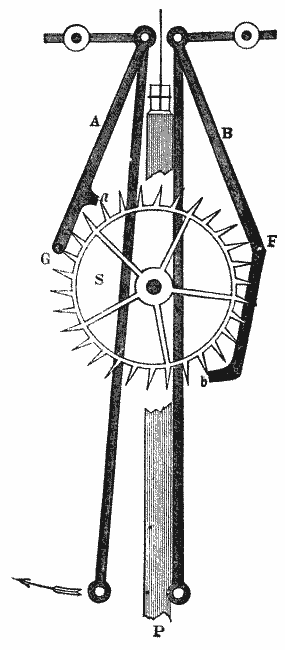
\includegraphics[height=0.7\textheight]{images/fig31.png}\index{Ritchie's electrical clocks}
\label{fig31}
\end{figure}

In this figure~(\ref{fig31}) the pendulum is returning from the
extreme right, and has just deposited the right pallet, $\mathrm{BF}b$
with its end pressing on the
tooth at $b$, and so trying to
turn the wheel that way.
But it cannot turn until the
pendulum has gone farther
and lifted the left pallet
which is now locking the
wheel at $\mathrm{G}$\@. As soon as it
does that, the weight of $\mathrm{B}$
moves the wheel, and itself
falls a little more until
another tooth locks at $\mathrm{F}$\@.
Then the left pallet falls
and presses on a tooth at
$a$, but cannot move the
wheel until $\mathrm{F}$ is unlocked,
and so on. In large clocks
exposed to wind, a click is
added to prevent the wheel
from being blown backward
by a force of wind greater
than the weight of each
pallet for the moment; it
cannot be blown forward
by reason of the stops $\mathrm{FG}$\@.

As the secondary clocks
are kept in order by the
normal one, they will bear
\markboth{SHORT AND SLOW PENDULUMS.}{SHORT AND SLOW PENDULUMS.}a short or slow pendulum on
the principle described at p.~\pageref{subsec:Short_and_slow_pendulums.}; and so a clock with a one or
%-----File: 175.png--------------------------------------------
%-----Folio: 160-----------------------------------------------
even a two seconds pendulum can be comprised in the length
of an ordinary half-seconds `dial,' as they call those very short
\begin{figure}[htbp]
\centering
\hypertarget{fig32}{\caption{\sc Ritchie's Pendulums}}
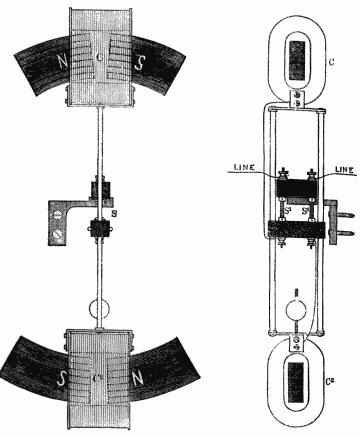
\includegraphics[width=\textwidth]{images/fig32.png}\index{Ritchie's electrical clocks!their pendulums}
\label{fig32}
\end{figure}
clocks, which look no bigger than their dials. Accordingly
Mr.~Ritchie makes these pendulums, as in this figure~(\ref{fig32}).
%-----File: 176.png--------------------------------------------
%-----Folio: 161-----------------------------------------------
The lower half of the pendulum is rather longer than the
upper, but both have bobs of wire coils in a cylinder, passing
over a set of magnets as before described. The suspension is
by two springs at $\mathrm{S}$, as shown in the right hand part of \hyperlink{fig32}{this
figure}, which is the section across the plane of vibration;
and one is connected with one battery wire, and the other
with the other, the pendulum itself being made with two
rods; and so the current goes down one and up the other,
being reversed at each beat as before. In this way also a
double attraction is got, as both bobs act in the same way.
The small ball above the lower bob is for regulating the
pendulum. The left hand figure is the front view.

This is taken in substance from a paper by Mr.~Ritchie
read to the Royal Scottish Society of Arts in April 1873,
and published separately. His clocks are in use in connection
with the Liverpool Observatory, besides Edinburgh
itself, and a variety of other places. The great objection to
having all the clocks of any large establishment worked by
only one is the possibility of all time coming to an end by
any temporary failure of the one which `makes' the time
of all. It would be prudent to have two normal clocks
always ready to be connected with all the subordinate ones
in case one has to be stopped; and the normal clocks should
be good ones capable of going without any control.

When the last edition of this book was published, the
Royal Institution, which is a sort of head-quarters of
electrical science, had just been converting all its clocks into
electrical ones, not on any of the controlling plans, but on a
driving one, by currents from a sort of small turret clock
with a hollow electrical coil for a bob, swinging a very large
arc over two permanent magnets. As I expected, and intimated
then, it turned out a failure, and was given up after
a few years.

Another controlling plan is Lund and Blockley's\label{lund}, in which a
$\bigwedge$-shaped fork is brought down over the minute hand exactly
%-----File: 177.png--------------------------------------------
%-----Folio: 162-----------------------------------------------
at the hour by electrical connection with a standard clock, so
as to bring it to the time if it is a little out either way. That
requires a complete clock wound up and going as usual, only
it need not go very well independently. There are also clocks
driven by pneumatic connexion with a standard one; but I
have no authentic information about their success.

\subsection[Time balls and guns]{Time balls and guns}\markboth{ELECTRICAL TIME BALLS.}{ELECTRICAL TIME BALLS.}\label{subsec:Time_balls_and_guns}\index{Time balls and guns}\ are let off by electrical connection
with a normal clock which attracts an armature on a trigger
which lets off the ball or fires the gun when the connection is
completed by contact springs in the $12$ or $24$~hour wheel and
the minute wheel simultaneously. In like manner the Westminster
clock reports itself to Greenwich daily. A time ball
is usually a large wicker globe covered with painted canvas,
fixed to a piston which falls down into a bell-mouthed tube
just air-tight enough for the air to act as an elastic cushion.
It is hauled up by hand a few minutes before the time for
falling. But these also sometimes fail like electrical clocks,
and a better plan is to let a common strong clock electrically
controlled discharge the ball or gun mechanically, just as it
lets off a striking part.

\section{STRIKING CLOCKS.}\label{sec:STRIKING_CLOCKS.}\markboth{CLOCKS STRIKING ONE.}{CLOCKS STRIKING ONE.}\index{Clocks!striking}
\index{Striking clocks}\index{Striking part!of house clocks}
The simplest form of a striking clock is represented in
fig.~\ref{fig33}. It only strikes one at every hour, which is sometimes
more agreeable than striking the full hour, especially
where you can easily see at once what the hour is. It is
very seldom that anybody has to count the striking of a
clock except in the night. Striking one requires no striking
part, or separate machinery to be wound up, the hammer
being lifted by a snail (or sometimes, but worse, by a pin)
on any wheel which turns in an hour, and dropped as the
minute hand reaches the hour. It cannot be done however
without affecting the friction of the clock, and therefore its
rate, except with a gravity escapement or some equivalent
%-----File: 178.png--------------------------------------------
%-----Folio: 163-----------------------------------------------
contrivance to prevent the inequality of force from reaching
the pendulum; and the remark I made at page~\pageref{squaring} about
the importance of fitting the dial spring on to the centre
arbor with a square instead of a round hole, applies still
more strongly here, as the friction of that spring has to overcome
\begin{figure}[ht!bp]
\centering
\caption{\sc Clock striking one at the hour}
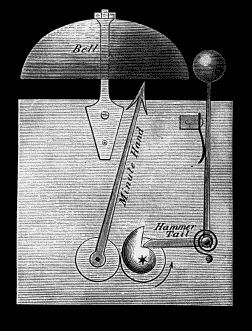
\includegraphics[width=0.7\textwidth]{images/fig33.png}\index{Striking part!of house clocks}
\label{fig33}\index{Clocks!striking!striking one at the hour}
\end{figure}
the resistance of the hammer spring. The short spring
against which the hammer shank falls is to prevent it from
jarring on the bell, and this is necessary in every case both
in large and small clocks, unless some other contrivance is
%-----File: 179.png-----------------------------------------------
%-----Folio: 164--------------------------------------------------
resorted to for the same purpose, such as I shall speak of
under turret clocks. In common clocks this check is given
\begin{figure}[htbp]
\centering
\hypertarget{fig34}{\caption{\sc Common Striking Clock}}
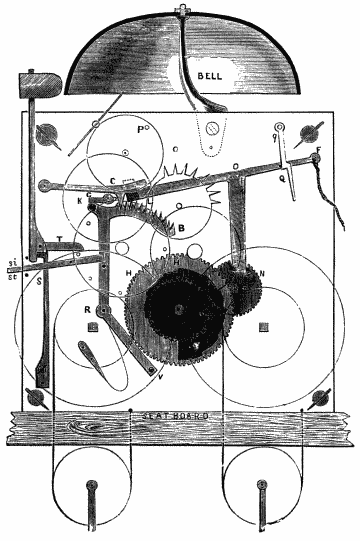
\includegraphics[width=\textwidth]{images/fig34.png}
\label{fig34}
\end{figure}
%-----File: 180.png-----------------------------------------------
%-----Folio: 165--------------------------------------------------
in a simpler way, as shown in fig.~\ref{fig34}, where the square top
of the stiff spring $\mathrm{S}$ butts against the square piece on the
hammer shank, whose own elasticity lets the hammer strike
the bell and then pulls it back again just out of contact. A
piece of vulcanised India rubber tied round the pillar also
answers very well.

\hyperlink{fig34}{This figure} is a front view of the common construction of
an English\index{Clocks!striking!English or repeating striking work}\markboth{ENGLISH OR REPEATING METHOD.}{ENGLISH OR REPEATING METHOD.}\label{repeat}\index{Repeating striking work} striking clock: the foreign ones are different, as
I will explain presently. The wheels shown only by circles
(with a few of the scapewheel teeth) are within the frame;
only those with teeth are outside, and they are indicated by
the same letters as in p.~\pageref{fig25}. The hammer tail is raised by
$8$ pins in the second wheel of the striking train, which corresponds
to the centre wheel of the going train. The pinion
of that wheel generally has $8$ leaves, and is driven by the
great wheel of $78$, which therefore turns in $12$~hours; not
that that is at all material, and of course higher numbers
would be better. The striking wheel drives the wheel
above it once round for each blow, and that wheel drives a
fourth (in which you see a pin $\mathrm{P}$) six or any integral number
of turns for one of the third wheel, and the fourth wheel
drives a fly to moderate the velocity of the train and the
time of striking.

The number of blows to be struck is regulated thus: the
dial-wheel $\mathrm{N}$ has a pin on its face which raises the \textit{lifting
piece} $\mathrm{LONF}$ a little before the hour, just far enough for it to
lift the long click $\mathrm{C}$ out of the teeth of the \textit{rack} $\mathrm{BKRV}$,
which then falls back (helped by a spring at its tail) as far
as the tail $\mathrm{V}$ can go by reason of the position of the snail $\mathrm{Y}$
on the hour-hand wheel $\mathrm{H}$; which has steps in it, one for each
hour, so as to let the rack fall the distance of one of its own
teeth for every hour the clock ought to strike. This fall of
the rack makes the noise called \textit{warning} a few minutes
before the clock strikes. The reason why it cannot begin to
strike yet is that the pin $\mathrm{P}$ cannot pass a stop which is
%-----File: 181.png-----------------------------------------------
%-----Folio: 166--------------------------------------------------
turned inwards from the lifting piece, through a large hole
in the frame, until that piece drops again, which it does
exactly at the hour by the advance of the pin in wheel $\mathrm{N}$\@.
Then the striking train is free, and that little piece $\mathrm{KG}$,
called the \textit{gathering pallet}, which is squared on to the prolonged
arbor of the third wheel, gathers up the teeth of the
rack, one for each blow of the hammer: the click is lifted as
each tooth passes, and prevents the rack from falling again,
and at last all the teeth are gathered up and the tail of the
pallet is stopped by the large pin $\mathrm{K}$ in the top of the rack,
and the train can go no further.

The great feature of this English striking work is that you
may `strike'\markboth{REPEATING STRIKING WORK.}{REPEATING STRIKING WORK.} the clock as often as you like within the hour,
or stop it any number of hours, and yet it will always strike
right, because the striking depends on the position of the
snail attached to the going part, and not at all on the number
last struck. These clocks are therefore sometimes furnished
with a string to the outside, from the click, so that you can
pull it in the night and hear the hour. But this is just the
wrong way of doing it: for if you hold the string too long
the click will miss some of the teeth and the clock strike too
many, and if you drop it too suddenly the rack will not
have fallen its full distance and it will strike too few. The
right place therefore to put the string is to the lifting piece,
as at $\mathrm{F}$\@. (The piece $\mathrm{Q}q$ belongs to something else which I
shall speak of presently.)

The improved French\label{newfrench}\markboth{NEW FRENCH STRIKING WORK.}{NEW FRENCH STRIKING WORK.} clocks, whose escapement I noticed
at p.~\pageref{subsec:Improved_French_clocks.}, have a better mode of stopping the striking than
the usual one in English house clocks: the better one is used
in our turret clocks when they have the rack movement.
Instead of the gathering pallet $\mathrm{G}$ (fig.~\ref{fig32}) on the third wheel
of the train being stopped by a pin in the tail of the rack
with a heavy blow, the striking is stopped by the pin $\mathrm{P}$ in
the fourth wheel coming against a stop in the long click $\mathrm{C}$,
which drops into a deeper notch in the rack than the others
%-----File: 182.png-----------------------------------------------
%-----Folio: 167--------------------------------------------------
at the last blow of the hour, and so falls low enough to catch
that pin.

\subsection[Strike and silent.]{Strike and silent.}\markboth{STRIKE AND SILENT.}{STRIKE AND SILENT.}\label{subsec:Strike_and_silent.}\index{Clocks!striking!strike and silent}\index{Strike and silent}---There are several ways of throwing
the striking work out of gear, so as to keep the clock silent.
I think the best, though not the usual one, is that shown in
fig.~\ref{fig32}, a small lever whose end $x$ falls before and stops a
pin in the rack when the other end of the lever is put up to
$si$ by an index or handle coming through the edge of the
dial. I have seen methods used which are very likely to
stop the going as well as the striking of the clock by leaving
the rack to fall. Another way is to make the piece $\mathrm{LONF}$
push forward so as to escape the pin at $\mathrm{N}$, and be never
lifted; and this is unobjectionable.

It may save people a little time if I tell them what hardly
anybody seems to know, that you may move the hands of an
\textit{English} clock forward through all the hours without waiting
for any of them to strike, except $12$, where the rack-tail has
to get over the great step in the snail; and even that is
often provided for by sloping the front of that step and the
face of the pin $\mathrm{V}$, to let the snail push it aside, the tail being
elastic enough to give way a little. In the same way the
tail of the lifting piece at $\mathrm{N}$ is always twisted a little to let
the lifting pin pass it backwards without lifting, so that you
may turn the hands back and the clock will not strike at all,
unless it has already given warning. The snail is sometimes
set on a separate wheel below the hour-wheel and moved by
jumps by a pin in the minute-wheel $\mathrm{M}$; this is called the
\textit{star wheel} and \textit{jumper;} but I can see no use in it, and therefore
shall describe it no further.

\subsection[Locking-plate striking work.]{Locking-plate striking work.}\markboth{LOCKING-PLATE STRIKING WORK.}{LOCKING-PLATE STRIKING WORK.}\label{subsec:Locking-plate_striking_work.}\index{Clocks!striking!foreign or locking-plate method}\index{Locking-plate movement}---The principle of the
striking work still used in most foreign clocks, French, German,
and American, is shown in fig.~\ref{fig35} (p.~\pageref{fig35}), though the
actual arrangement of the pieces may be different. It is
generally used also in English turret clocks. You see the
rack and its click are gone, and instead there is a wheel $\mathrm{Y}$
%-----File: 183.png-----------------------------------------------
%-----Folio: 168--------------------------------------------------
called the locking plate or count wheel, which turns in the
$12$~hours, and may therefore be put on the arbor of the
great striking wheel, or driven by the pinion of the striking
\begin{figure}[htbp]
\centering
\caption{\sc Locking Plate Striking}
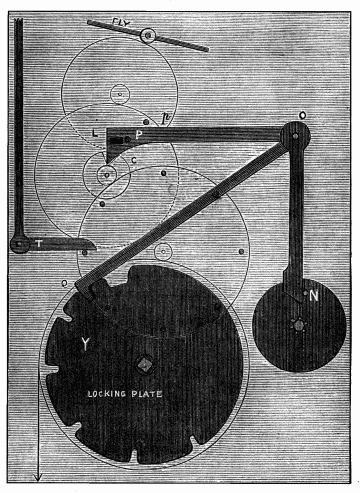
\includegraphics[width=\textwidth]{images/fig35.png}
\label{fig35}
\end{figure}
%-----File: 184.png-----------------------------------------------
%-----Folio: 169--------------------------------------------------
wheel. It may be considered as marked out into $78$ divisions,
and notches made in it at the distances $1$, $2$, $3$, \&c.,
into which a lever $\mathrm{OQ}$ can drop, which is connected with
the lifting piece. That is generally made with two stops
upon it, one a little behind and below the other; or else
there are two levers, one lifted by the other, with the stops
upon them respectively; and the pin $\mathrm{P}$ in the pin-wheel, or
in large clocks, on the fly arbor, stops against the first when
the clock has done striking, and against the other when the
lifting piece is lifted by the wheel $\mathrm{N}$ in the dial work. But I
introduced an \markboth{IMPROVED CONSTRUCTION.}{IMPROVED CONSTRUCTION.}alteration in this respect in turret clocks,
because one of the stops on the lever must be out of the
right position for direct action of the pin. Instead of two
stops on the lever, there are two pins on the wheel, $\mathrm{P}$ and $p$,
one a little behind and nearer the centre of the wheel than
the other, and $p$ is caught by the stop when it has been lifted
high enough to let $\mathrm{P}$ escape and `give warning.'

There is, or ought to be, a disc $\mathrm{C}$ with a notch or cam
in it on the arbor of the third wheel, which turns once for
each blow, and so moves faster than the locking plate, and
therefore is more certain to lift the lifting piece quite out of
the way of both pins before the pin-wheel gets once round;
otherwise the clock might be, and clocks without this cam
sometimes are, prevented from striking at all, especially if
the parts are not adjusted with great precision. The lifting
piece evidently cannot fall again until another notch in the
locking plate comes under the tooth $\mathrm{Q}$\@. Sometimes the
lifting piece $\mathrm{LON}$ is made in two pieces, one lifting the
other, but I see no advantage in it, except where the pivot
$\mathrm{C}$ happens to be at an inconvenient distance from the locking
plate. In turret clocks with three-wheeled trains it is
generally more convenient to make the wheel $\mathrm{C}$ turn only
half round for each blow, and then there must be two cams
or two drops in the disc, as shown in the view of a large
quarter clock at p.~\pageref{fig40}.
%-----File: 185.png-----------------------------------------------
%-----Folio: 170--------------------------------------------------

\subsection[Half-hour striking.]{Half-hour striking.}\markboth{HALF-HOUR STRIKING.}{HALF-HOUR STRIKING.}\label{subsec:Half-hour_striking.}\index{Beckett, Sir E.!half-hour striking}\index{Clocks!striking!half-hour striking}\index{Half-hour striking}\index{Striking clocks!half-hours}---For striking \textit{one} no lift by the
locking plate is required, but only a long notch reaching
from $12$ to $2$; and for the same reason the clock can be
made to strike one at the half hours by dividing the locking
plate into $90 (=78+12)$ and leaving a wide notch between
every two hours, and putting a half-hour pin into the wheel
$\mathrm{N}$ (fig.~\ref{fig32}) besides the hour one. Most of the French clocks
are so made; but they have the inconvenience of striking
one three times between $12$ and $2$; so that between those
hours the striking tells you nothing. I once saw a turret
clock made to strike one feebly on a smaller bell, from the
going part, as shown at page~\pageref{fig33}, which gravity escapement
clocks will bear, though not others. It was not satisfactory,
and led me to devise the following plan.

To make $12\frac12$ and $1\frac12$ silent, with the locking plate
movement, we evidently want something which will stop
the lifting piece, $\mathrm{LON}$ in fig.~\ref{fig37} (p.~\pageref{fig37}) of a clock of this
kind, from falling after it has been lifted to give warning,
until the next hour. And the way to do that is to have a
$12$-hour wheel (the one with $24$ ratchet teeth in fig.~\ref{fig37})
with two steps in it, as you see, which come under the
tongue of the lifting piece just over that wheel at those two
half hours. The best way to drive it is by a gathering pin
or single tooth, which is shown in the hour wheel marked
$40$, and which moves the ratchet wheel one tooth just after
warning. There is also a spring click or jumper to keep it
in its place, which wheels driven in that way always require,
to make sure of the gathering tooth taking them up again.
But another thing has to be attended to. The locking plate,
instead of having $78$ teeth or spaces, as when there are no
half hours, or $90$, as when all the half hours strike, must
have $88$, and each notch must again be wide enough for
striking one, only it must be divided as if there were no half-past
twelve or one, for one o'clock is the same as one half
hour between twelve and two.
%-----File: 186.png--------------------------------------------
%-----Folio: 171-----------------------------------------------

\subsection[Half-hours with Rack Movement.]{Half-hours with Rack Movement.}\markboth{DIFFERENT METHODS OF DOING HALF-HOURS.}{DIFFERENT METHODS OF DOING HALF-HOURS.}\label{subsec:Half-hours_with_Rack_Movement.}\index{Half-hours with rack movement}---I have never
seen this in any English clock. Indeed the English house
clock-makers seem determined to lose every bit of the trade
rather than allow any single improvement to be made here,
and so they are losing more and more yearly. The modern
French\index{French clocks!improved kind of} arrangement of the rack movement has the rack
above the `motion' or dial wheels, acting by gravity without
a spring, and the striking is stopped by the long click dropping
lower at the end of the rack than it does in the teeth,
and low enough to catch a pin in the third wheel, instead of
the gathering pallet being stopped by a pin in the rack and
always tending to force it back. Half hours are struck by a
separate lever being brought under a pin anywhere on the
rack allowing it to fall one tooth only, the lifting piece being
of course lifted by a second pin in the hour wheel at the half
hours. In order to stop the striking at $12\frac12$ and $1\frac12$ there
would have to be a $12$-hour wheel with $2$ steps or long teeth,
as before described, to prevent either the rack or the lifting
piece from falling, whichever might be most convenient.
But this is not of so much use in small clocks standing in a
room, when you can look up and see whether it means one
o'clock or not, as in large ones, where it is a great convenience,
and saves the much greater cost of quarters with
the two more bells. It would never do to have a turret
clock striking the hours on one of the quarter bells, as it
would produce frequent confusion when they are heard at
such a distance that people would not be sure whether they
heard the smaller bell or not. It was done for some months
at Westminster by the genii who managed and advised things
there, as will be noticed afterwards. When Mears's Big
Ben II.\ cracked enough to spoil the sound, but no more,
they stopped the striking of the hours on him, and had them
struck on the fourth quarter bell, until I got the confusion
that it caused noticed in the newspapers, and then they
resumed striking on the great bell with a much lighter
%-----File: 187.png--------------------------------------------
%-----Folio: 172-----------------------------------------------
hammer, which is there still. And for fear that should knock
a piece out of it, like the one in the famous broken bell of
Moscow, they put a huge wooden tea-tray under it to catch
the piece, and there it is to this day, with a hole in the
middle for the clapper `tail to come through,' which reminds
one of a celebrated poem of either Southey or Porson, for it
is attributed to both.

The locking\index{Locking-plate movement} plate striking is specially objectionable for
moveable clocks, and for any that are liable to run down
for want of winding, like the American ones; because if
the striking once gets wrong, or stopped from not winding
up, or let off by accident, or the clock stopped by housemaids,
it strikes wrong afterwards, until it is struck round
to the right hour again. The American clocks have a wire
specially provided for this purpose, but the French have not,
and you have to put your finger in behind the left side of
the clock and lift the lever you will feel there, to make it
strike as often as is necessary to bring it right; which is a
great nuisance, and in some cases almost or quite an
impossibility. Striking on springs is a bad imitation of a
large bell, and is very inferior to a common bell, except
when heard very near.

\subsection[Quarters.]{Quarters.}\markboth{QUARTER CHIMES.}{QUARTER CHIMES.}\index{Clocks!striking!striking quarters}\label{quart}---If the clock is to strike the quarters, a third
`part' or train of wheels is added on the right side of the
going part, with as many bells and hammers as may be
required. There is indeed a method of making the same
striking part do both for the hours and quarters, by sliding
the hour hammer tail out of gear with the pins, and the
quarter hammer tails into gear, and \textit{vice vers\^a;} but it
saves very little in cost, and is very seldom used; and
it requires a much heavier weight or stronger spring, and
stronger wheels, if it is to be done effectively. In that case
there can be no quarters at the hour; but that is of no consequence,
and perhaps rather an advantage with \textit{ding dong}
quarters. The construction of a quarter part is substantially
%-----File: 188.png--------------------------------------------
%-----Folio: 173-----------------------------------------------
the same as of the hour striking part. If there are only $2$
bells, the $2$ hammers are lifted by pins on each side of the
striking wheel, or they may be the same pins if the arbor of
one hammer is put above that of the other. They should
be so placed that the interval between each pair of blows, or
each chime, is twice that between the blows of each chime,
whether there are $2$ or $4$ bells. When there are more, the
interval between each chime requires to be as much as $3$
spaces instead of $2$. When there are more than $2$ bells the
hammers are worked by a chime barrel, because the chimes
are not generally the same thing repeated, as they are
with \textit{ding dong} quarters. But this belongs more to turret
clocks, under which I shall go more fully into it. The
chime barrel is generally put on the third wheel, but it would
require less force to turn it on the second, for the reason
I gave before, that the more wheels there are between a slow
power and a quick work, the more is lost in friction, in a proportion
beyond what anybody would expect. As the barrel
naturally turns in an hour, the proportion of the pinion and
great wheel would be just the same as in the going part.

The quarters may be let off either by the English
repeating method, or by the French locking plate. If they
are merely the same chime repeated $2$, $3$, and $4$ times, the
repeating movement should be used, as it has the same
advantage as in the hour striking part. But if each quarter
is a different tune, it should not be used, because repeating
the striking of the quarters in that case will throw the whole
tune into confusion; though this plain distinction is often
overlooked. The connection between the two striking parts,
when the quarters have the locking plate, is made by that
wheel performing the function of the wheel $\mathrm{N}$ in figs.~\ref{fig34}, \ref{fig35},
in discharging the hour, as the 4th quarter finishes.

The repeating\index{Quarter chimes!rack and repeating movements in small clocks} quarter movement is not so simple: the
principle of it is this:---The quarters have a rack, snail, \&c.,
just like the hours, the snail being fixed on the wheel $\mathrm{N}$ so
%-----File: 189.png--------------------------------------------
%-----Folio: 174-----------------------------------------------
as to turn in the hour, and with $4$ steps instead of $12$ (see
p.~\pageref{fig34}). The rack is so placed that when it falls for the 4th
quarter (its greatest drop) it falls against the hour lifting
piece somewhere between $\mathrm{O}$ and $\mathrm{N}$, so as to raise it and
the click $\mathrm{C}$\@. It is then held up by the lever marked $\mathrm{Q}{q}$
catching hold of the pin close by it, and as the last tooth
of the quarter rack is gathered up it pushes $\mathrm{Q}q$ aside again,
which lets the lifting piece drop and the hour begin to strike.

There is a very simple construction of a \markboth{QUARTER CLOCKS.}{QUARTER CLOCKS.}clock for striking
repetition quarters only, when it is wanted in the night, by
pulling a string which goes round a spring barrel, and so\label{wind}
winds it up as far as it is allowed to go by the position of
the quarter snail on the going part, which stops some pin or
lever connected with the barrel. This may be easily made
to indicate half quarters; for if there are $8$ steps in the snail,
then at about $50$~min.\ past the hour the lever could go
$7$ depths and the clock would strike $3$ \textit{ding dongs} and one
bell more; and it may either begin or end by letting off the
hour. This construction is in substance that of \textit{repeater}
watches, of which the striking part is both wound up and
let off by pushing in the handle.

\subsection[Quarters--Tunes.]{Quarters--Tunes.}\markboth{QUARTER CHIMING CLOCK.}{QUARTER CHIMING CLOCK.}\label{subsec:Quarters--Tunes.}\index{Tunes, chime}---By this I mean chimes\index{Chime-tunes} not merely
repeated. And as these clocks for halls and rooms have
come much more into fashion since the Westminster chimes
were heard, I will give a picture of the construction I
arranged for them in a clock of my own before I designed
that clock, and which was followed in several others made
by old Mr.~Dent and afterwards by other makers. The chime
tunes themselves I shall leave till we come to turret clocks.
$\mathrm{Y}$, the locking plate, is fixed on the arbor of the second wheel,
which turns once in an hour, driving the chime barrel marked
$50$ for Westminster chimes, as will be explained afterwards.
For the present it is enough to say that it turns twice in the
hour, making $10$ chimes, but the fourth and first quarters
together are the same as the second and third together, and
%-----File: 190.png--------------------------------------------
%-----Folio: 175-----------------------------------------------
\begin{figure}[htbp]
\centering
\hypertarget{fig36}{\caption{\sc Quarter Chimes, Striking Part}}
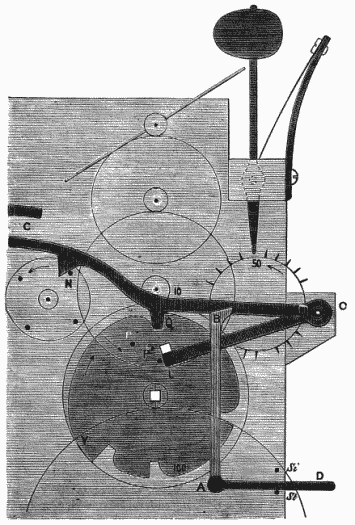
\includegraphics[height=525pt]{images/fig36.png}
\label{fig36}
\end{figure}
%-----File: 191.png--------------------------------------------
%-----Folio: 176-----------------------------------------------
therefore it is not necessary to have a barrel with $10$ different
sets of pins on it, but only $5$. The wheel on its end therefore
has $50$ teeth, and is driven by the second wheel of the
train, of $100$, which also drives a pinion of $10$ on the third
wheel, which consequently turns once for each chime of
$4$ bells. That wheel also has two pins in it, $\mathrm{P}$ and $\mathrm{P}'$,
$\mathrm{P}$ being rather nearer the centre, and they are alternately
stopped by the piece at $\mathrm{L}$ projecting sideways from the
lifting detent $\mathrm{LON}$, of which the arbor is carried in cocks
from the frame, as you see, its arm $\mathrm{OQC}$ being in front of
the front plate of the clock and $\mathrm{OL}$ inside, near the back
plate where the third wheel is. The chime barrel is also
really set in cocks, not in the solid frame, in order that
it may be adjusted as to its teeth after the clock is put
together, which often saves a great deal of trouble, but it
would confuse the figure to show them \hyperlink{fig36}{here}. The fly should
be longer than will go inside the frame, to clear the arbor
below it, and that also is set in a long cock behind.

The action is extremely simple. The $4$ pins in the hour
wheel $\mathrm{N}$ lift the long detent a little before each quarter, and
then the pin $\mathrm{P}'$ slips under the stop $\mathrm{L}$, which then catches
$\mathrm{P}$, the wheel moving on a very little. At the quarter the
detent drops off $\mathrm{N}$, and before the third wheel or its pins
come round again the locking plate has lifted the detent by
the inclined edges of its notches, such as $\mathrm{Q}$, so high that both
pins clear the stop $\mathrm{L}$; the motion of the locking plate \hyperlink{fig36}{here}
being much greater than in an hour striking plate like fig.~\ref{fig35} and figs.~\ref{fig37}, \ref{fig40} afterwards, where consequently a cam
wheel turning faster is required to make the lifting safe.
The locking plate keeps up the detent for $1$, $2$, $3$, or $4$ chimes
as required, and you see that by this method they can never
get mixed, as they can with the repetition or rack movement.
If they have got to strike wrong they only want `striking
round' till they are right again, and that is easily done
thus. You see the right-angled lever $\mathrm{BAD}$, with $Si$ and $St$,
%-----File: 192.png-----------------------------------------------
%-----Folio: 177--------------------------------------------------
for \textit{silent}\index{Strike and silent}\markboth{STRIKE AND SILENT.}{STRIKE AND SILENT.} and \textit{strike}\index{Clocks!striking!various mechanisms for striking work}, against two pins in the frame. When
you lift the tail $\mathrm{D}$ to $Si$ the bevelled end $\mathrm{B}$ lifts the detent by
a pin in it, just enough to `give warning,' and it cannot fall
again. But when you bring it down again to $St$ the detent
does fall and the quarters strike whatever the locking plate
is ready for, which lets you know whether they require
more `striking on' to set them right.

But we have still to let off the hour\label{hourstrike} striking. In large
clocks that is best done independently, as we shall see; but
in small ones it is done by the end of the detent being
raised by the snail kind of rise at $\mathrm{Y}$ in the locking plate
as the fourth quarter finishes, which lifts $\mathrm{C}$, the rack
click of the striking part (see fig.~\ref{fig34}). That is one way of
doing it. Another, which I designed for a later clock of my
own, allows the hours to strike even if the quarters are
silenced, by retaining the usual lifting piece of the hours
(which in the former plan is gone) and making the quarter
detent stop it from falling again till the quarters are done---if
they are in action; if not it simply does nothing. The
quarters are silenced by pressing a spring against the side of
the fourth wheel, by a slider at the edge of the dial.

\subsection[Alarums.]{Alarums.}\markboth{ALARUMS.}{ALARUMS.}\label{subsec:Alarums.}\index{Alarums}---If you suppose a short hammer instead of a
pendulum fixed to the pallet arbor or the crutch of either
kind of recoil escapement, it would swing backwards and
forwards very quickly, and strike both sides of a bell of
proper size placed so as to inclose the hammer. This is the
way an alarum strikes, and not by the lifting of a hammer at
distinct intervals. The hammer is driven by a wheel like a
strong recoil crown escapement wheel (p.~\pageref{crown}) with a spiked
pulley or barrel attached to it by a ratchet and click, over
which a rope goes, with a small weight at one end, and a
smaller one at the other to keep the rope stretched and to wind
it up by. The alarum can only go when a stop lever is lifted
by a pin on a collar which is fixed on the hour hand wheel
by a friction spring, so that it can be set to go off at any hour
%-----File: 193.png-----------------------------------------------
%-----Folio: 178--------------------------------------------------
you like. You must not wind it up till within $12$~hours of
the time it is intended to go off, or it will go $12$~hours too
soon.

\subsection[Tell-tale clock]{Tell-tale\index{Clocks!tell-tale} clock.}\markboth{TELL-TALE CLOCK.}{TELL-TALE CLOCK.}\label{subsec:Tell-tale_clock}\index{Tell-tale clocks}---This is said in one of the Parliamentary
papers about the Westminster clock to be an invention of
Mr.~Whitehurst of Derby, for watching watchmen and telling
whether they are on the watch and in the proper place all
the night. That unpleasant little clock which one hears
striking the quarters $3$ or even $4$ times in some Westminster
Abbey sermons, is of this kind, and there are some in
the lobbies of the Houses of Parliament. There are a set of
spikes sliding in holes in a $24$~hour dial, one for every
quarter of an hour, which can be pushed in by pulling a
handle in the clock case during a few minutes of that quarter
only. So if any pin is found sticking out in the morning it
indicates that the watchman was either asleep or away at
the time belonging to that pin. The plate carries the inner
ends of the pins over an inclined plate or roller at some other
period of the $24$~hours, which pushes them all out again
ready for work the next night.

\subsection[Musical clocks.]{Musical clocks.}\markboth{MUSICAL CLOCKS.}{MUSICAL CLOCKS.}\label{subsec:Musical_clocks.}\index{Clocks!musical}\index{Musical!clocks}---Clocks that play tunes---not short
quarter chimes, but tunes of several minutes, either on bells
or organ pipes, are not clocks in respect of their music, but
simply musical boxes or barrel organs turned by an independent
spring or weight and let off at the required time by
a lever from the clock. I shall speak of chimes on church
bells farther on. And nothing else occurs to me as
belonging to small or house clocks of sufficient use or
importance to require notice. So I pass on to the larger
branch of the art, which has been the subject of greater
improvements within the last 30 years than in the previous
century, and has reached a degree of accuracy equal to that
of the best astronomical clocks, and superior to that of
chronometers, and that not only without an increase, but
with a great reduction in the price.
%-----File: 194.png--------------------------------------------
%-----Folio: 179-----------------------------------------------
\section{CHURCH OR TURRET CLOCKS.}\label{sec:CHURCH_OR_TURRET_CLOCKS.}
\index{Turret clocks}\markboth{TURRET CLOCKS.}{TURRET CLOCKS.}
It may be supposed that as the work of these clocks only
differs from that of house clocks in the size of the hands
and the weight of the hammers they have to move, you
have only to enlarge the machinery and the business is done.
But there is a very important fact in the way of that
conclusion: viz., that as you increase the strength of
machinery you increase its weight in a ratio as much higher
as the cube is higher than the square of any of its
dimensions; and when you increase weight you increase
friction,\index{Friction!in turret clocks} and friction is a word which ought never to be long
out of the mind of a clockmaker, or at least of a clock-designer,
inasmuch as the timekeeping part of a clock is the
only machine whose sole business is to overcome its own
friction, resistance of the air, and variations of heat, and to
do that in a constant and uniform manner. And there is
this further difference\index{Large and small clocks, difference between} between large and small clocks: in
small ones the force or weight required to work a hammer
of an ounce or two is generally about the same as is required
to keep the pendulum going, and so the two `parts' or
trains are about equal in strength; whereas in large clocks
the lifting of the hammer generally requires a great deal
more power than driving the hands and pendulum, and therefore
ought to have much heavier and stronger machinery.
Nevertheless the object of some clockmakers seems to be to
make the going train of large clocks as heavy and the
striking train as light as they can.

\subsection[Pendulum.]{Pendulum.}\markboth{CHURCH CLOCKS.}{CHURCH CLOCKS.}\label{subsec:Pendulum.}\index{Pendulums!for church clocks|(}---I have already treated of pendulums for
large as well as small clocks at considerable length, and
there is little to add with reference to large clocks only. I
will only repeat that the construction and suspension of the
pendulum are of primary importance.

The great majority of clockmakers, till lately, set their
faces against compensated pendulums\index{Compensation of pendulums}, and used nothing but
%-----File: 195.png--------------------------------------------
%-----Folio: 180-----------------------------------------------
wooden ones. And so long as the clocks themselves are no
better than they are, it would undoubtedly be a waste of
money to compensate the pendulums, as the escapement
errors will far exceed the temperature one. But when you
have got a first-rate clock in other respects, it is absurd to
prevent it from going accurately by not giving it a pendulum
without which it cannot keep the same rate in hot
and cold weather. It is true that a $2$~seconds, or even a
$1\frac12$~second compensated heavy pendulum, is a rather expensive
affair if well made; and with a common dead escapement
probably the advantage is on the whole in favour of a
$13$~ft.\ wood pendulum of $3$~cwt.\ over a $5$~ft.\ compensated
one of half the weight, which will enable a clock with such
an escapement as I shall describe to keep within a second a
week of Greenwich time. The fashion of extravagantly
long pendulums has very properly gone out, as their
inconvenience and liability to be affected by the wind overbalances
any advantage from them in a moderately good
clock. There were several in Yorkshire until lately as long
as $56$~feet, or $4$~seconds: $20$~feet = $2\frac12$~seconds, which old
Doncaster church had, is the utmost length I should allow;
and I gave the calculations for a cheap form of compensated
pendulum of that length at p.~\pageref{pndcalc}.\index{Pendulums!for church clocks|)}

\subsection[Position of clock.]{Position of clock.}\markboth{POSITION OF CLOCK.}{POSITION OF CLOCK.}\label{subsec:Position_of_clock.}\index{Turret clocks!best position for}---The worst of all positions for a large
clock is the usual one, on a stool on the upper floor of a
tower, for the reason I have already given at p.~\pageref{stool}. The
best is on stone corbels built deep into the wall. The
Westminster clock lies on independent walls, which of course
are stronger still. Where this cannot be done, cast iron
brackets bolted through the wall will do, or iron beams
across the room if it is not very wide. Wooden beams are
not to be trusted. When the clock is fixed as firmly as
this, the pendulum may be hung from the clock frame, if
that is itself strong enough, and the pendulum cock properly
fixed to it, or cast with it, though the wall is generally to be
%-----File: 196.png--------------------------------------------
%-----Folio: 181-----------------------------------------------
preferred for a long and heavy pendulum, if the clock stands
near enough to it. But again it is inconvenient to have a
very large clock so close to the wall that a man cannot get
some access to it from behind. Therefore no general rule
can be laid down for the fixing of turret clocks, except that
firmness is the first consideration, to which everything else
must give way according to the circumstances of the tower.
I have already mentioned at p.~\pageref{arc} the increase of arc caused
by hanging a heavy pendulum from the wall instead of a
strong wooden frame from the ground; and as the escapement
errors vary inversely as the cube of the arc, the clock
should go more than twice as well with the firmer suspension;
and in fact it does.

\subsection[Frame.]{Frame.}\markboth{FRAME.}{FRAME.}\label{subsec:Frame.}\index{Frames!for turret clocks}\index{Turret clocks!frame for}---The old established form of clock frame was a
sort of cage of vertical and horizontal bars, some of which
contain the bushes for the pivots of the wheels, and have to
be unscrewed from the principal bars in order to get any of
the wheels out. It was a great improvement on this to fix
the bushes themselves with screws instead of riveting them
into the bars, as it enabled the wheels to be taken out
separately, instead of all dropping loose at once and perhaps
bending their back pivots as soon as the front bar was
taken off. Mr.~Vulliamy\index{Vulliamy, Mr.} introduced this plan, and old Mr.
Dent used it in the Exchange\index{Exchange, Royal!clock} clock, of which a perspective
view is given in Tomlinson's Cyclop\ae dia under \textit{Horology}.
But he soon afterwards adopted a still better arrangement,
borrowed in principle from the French, who were strangely
ahead of us in this branch of clockmaking, until shortly before
the 1851 Exhibition.

The French\index{French clocks!improved kind of} clockmakers are entitled to the credit of
having introduced the horizontal frame cast in one piece,
with the great wheel set in bushes or cocks below it, and the
smaller wheels above in separate frames of the A~shape
bolted to the great one. But much more has been done
since that. Dent's\index{Dent, E.~J.!Exhibition clock} clock, with a spring remontoire, which I
%-----File: 197.png--------------------------------------------
%-----Folio: 182-----------------------------------------------
\label{folio_182}designed for him for the 1851 Exhibition, where it kept better
time\index{Gravity escapements!rate of some}\index{Rate!of some other gravity escapement clocks} than had ever been attained before, for nearly $6$~months,
will be described afterwards, though even that has been
superseded by the simpler and stronger construction of the
gravity escapement clocks. I will \markboth{SOME LARGE CLOCKS.}{SOME LARGE CLOCKS.}now describe a moderate-sized
turret clock of that kind, for a bell up to $5$ or $6$~cwt.,
and therefore only needing the striking part winding once a
week, which will not do for large ones, and striking one at
the ten proper half-hours as before described. This was
made for a clock-tower of my house by Mr.~Joyce\index{Joyce's turret clocks}\index{Turret and church clock makers}, of Whitchurch,
Salop, the maker of the great Worcester\index{Worcester cathedral!clock} Cathedral
clock, striking on a $4\frac12$-ton bell, and a vast number of
smaller clocks. I ought to mention at the same time that
Messrs.~Potts\index{Potts, maker of Lincoln Minster clock and others}, of Leeds, in 1881, put up a still larger one in
the finest clock-room in the world, about $40$~ft.\ square, in the
tower of Lincoln\index{Lincoln Minster clock} Minster, striking on Great Tom and four
new quarter bells; and Gillett and Bland\index{Gillett and Bland's!clocks and bells}, of Croydon, who
made the clock for some still larger bells in the Manchester\index{Manchester Town Hall clock and bells}
Town Hall. But all these, and a multitude of others not
quite so large, by these makers, and by Smith of Derby,
belong to the class which will be described afterwards,
winding every one or two days in the striking parts. Dead
escapements have now become quite obsolete for all large
clocks that are intended to keep time within the maximum
that ought to be allowed, viz.\ $5$~seconds a week; for I hear
that some of these large clocks do not vary $5$~seconds a
month, except from some temporary cause. Therefore,
although I retain the description and picture of one pattern
of a dead escapement clock farther on, the time is come to treat
the gravity escapement as the standard one for this purpose.
It is very easy too to make this next picture serve for a dead
escapement by putting the necessary A-shaped small frame
on to carry the pallets, making the third wheel which drives
the gravity three-legs into a dead pin wheel, as described at
p.~\pageref{fig15}.
%-----File: 198.png--------------------------------------------
%-----Folio: 183-----------------------------------------------

\begin{sidewaysfigure}[p]
\centering\index{Beckett, Sir E.!general plans for turret clocks}
\caption{\sc Small Turret Clock with Gravity Escapement}\index{Turret clocks!Batch-wood clock}
\label{fig37}
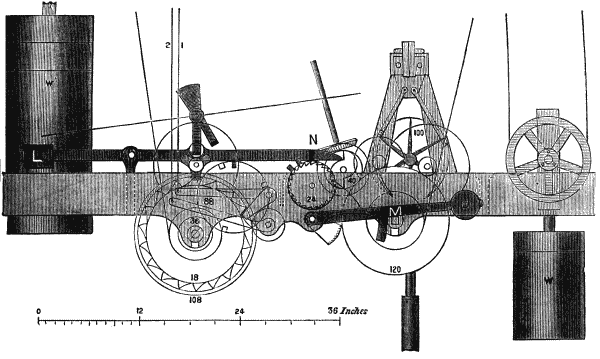
\includegraphics[width=\textwidth]{images/fig37.png}
\end{sidewaysfigure}
%-----File: 199.png--------------------------------------------
%-----Folio: 184-----------------------------------------------

Very few architects\index{Architects!ignore bells and clocks}\markboth{ARCHITECTS AND CLOCK-TOWERS.}{ARCHITECTS AND CLOCK TOWERS.}\label{architects} have the least idea, or will condescend
to learn, how large a clock-tower must be to hold a clock of
moderate size properly, or bells either. Their notion seems
to be that it is the duty of what they call their `clients'---they
being the `patrons,' I suppose---to let them build
what they think pretty, and then get other people to make it
useful if they can. I must inform their `unfortunate clients'
then, that they cannot have a clock of the best construction
suitable for a bell of only $4$ or $5$~cwt., and one or more dials
of $4$~ft.\ diameter, unless they provide a clock-room at least
$6$~ft.\ square, and $7$ is better, and at least $30$~ft.\ fall for the
weights. The frame\index{Turret clocks!frame for!its construction} in such a tower as that is best built
into the wall about half a brick deep at each end, as mine is,
and of course made quite level and firm. It will then be firm
enough to carry the pendulum, without resorting to an independent
cock built into the wall. Mine is about $3$~cwt., and just
$99$~in.\ long to the bottom, being $1\frac12$~seconds, which happened
to be more convenient than a $1\frac14$~seconds one, besides being
rather better. As it is generally necessary to carry the
ropes up to some place above the clock-room to get all the
available fall, you have to provide space for them also, and
evidently more than if they go straight down from the
barrels, which is better if you have fall enough, as it saves a
good deal of friction\index{Friction!in turret clocks} in several ways. This depends on the
height of the clock-room from the ground, and the use you
want to make of the lower part of the tower, which should
all be considered beforehand, but never is, except by people
who look after their own work, who alone get it done well.

Any \markboth{SMALL GRAVITY TURRET CLOCKS.}{SMALL GRAVITY TURRET CLOCKS.}one who is generally acquainted with clock-making
will understand from this picture more than could be shown
in it without confusion. The barrels\index{Turret clocks!iron barrels}, or great wheels of
both parts, are set under the frame in bushes of the construction
$a$ and $d$ together in p.~\pageref{fig38}, so that they can drive second
wheels in bushes of the form $b$ on the top of the frame,\index{Frames!for turret clocks}
which top is about $1\frac12$ wide, and is now always planed in a
%-----File: 200.png--------------------------------------------
%-----Folio: 185-----------------------------------------------
machine, to carry all the cocks and bushes quite firm and
level. There are three cross bars cast in it at convenient
places, which are utilized also for carrying cocks for `leading
off,' for hammer-tails, winding-pinions, and anything else of
that kind. The great going wheel\index{Turret clocks!three-wheeled trains} generally has \index{Wheels, numbers of teeth}$120$ teeth,
and is $12$ or $13$~inches in diameter, and drives (first) the hour
wheel with $40$ teeth, on the arbor of which is the bevelled
wheel driving other bevelled wheels up to the dials, both
outside the tower, as usual, and in mine inside also to a dial
at the end of a long passage in the house. That leading off
goes downwards obliquely, and is omitted in the picture.
The half-hour snails, with the main bevelled wheel, are
clamped to the hour wheel by thumb-screws, to enable you
to set the hands when necessary; and it drives no more
wheels in the train, because it makes a better distribution of
the teeth to leave it independent. The great wheel therefore
drives the one marked $100$ with a pinion of $10$, which will
turn in $15$~minutes as the $40$ wheel takes an hour, whatever
may be the time of the great wheel, which is generally made
$3$~hours in these clocks. The $15$~min.\ wheel of $100$ drives
another pinion of $10$, $\therefore$ in $1.5$~min., and that having a wheel
of $90$ drives the scape-wheel pinion of $9$, which, with the double
three-legs and a $1\frac12$-sec.\ pendulum, turns in $9$~seconds. But
if the pendulum is $1\frac14$ sec, the scape-wheel will turn in
$6 \times 1\frac14$ or $7\frac12$~sec., and its pinion must either be $8$ driven
by $96$ or $9$ driven by $108$.

In all clocks of this kind the pallet-arbors are set in small
cocks, on the large one which carries the pendulum, and the
scape-wheel itself has only a short arbor in $2$ cocks behind
the other wheels. The pendulum swings in a long slot in
the flange at the top of the frame, reaching from one cross
bar to the other; and the escapement fly also in another
space, with the two three-legged wheels between the back
bar and another which carries all the wheels. There is room
enough for all this, and a sufficient length of barrel, in the
%-----File: 201.png--------------------------------------------
%-----Folio: 186-----------------------------------------------
width of frame that the striking part requires, which is
always a good deal more than the going part, on account of
the greater thickness of the rope, and the cams and levers
and the winding wheel. The frame is generally $4\frac12$~in.\ deep,
with a wide flange turned inwards all along the top, to set the
various cocks on.

There is a little inconvenience in the third wheel turning
in $1\frac12$~min.\ instead of either $1$ or $2$, as you want an index of
some kind to mark seconds for regulating, unless you go
entirely by the striking. But this train distributes the teeth
so much the best that I adhere to it, and get over the other
difficulty either by a pair of small wheels in the proportion of
$3$ to $2$, the smaller carrying a seconds hand, or else depend
on an index placed over the rim of the $90$~seconds wheel,
which is graduated up to $30$, so as to give the seconds in
every half-minute, leaving you to see by the other dial, on
the hour arbor, which half-minute it is. With a $2$-sec.\ pendulum
there is no such difficulty; for the scape-wheel
then turns in $12$ sec, and its pinion of $10$ driven by a wheel
of $100$ lets that wheel turn in $2$~minutes; and that may have
a pinion of $10$ driven by $100$, which will turn in $20$~min.\ instead
of $15$, and consequently wants a pinion of $12$ to an
hour wheel of $36$. Several other numbers also would do;
but we shall see afterwards how the second wheel may
be used to obtain greater \index{Striking clocks!accuracy of discharge}precision in the time of beginning
to strike than you can get from an hour snail, a good way off
the escapement too, if the second wheel turns in $15$ or $20$
minutes. And if you want to apply it to the half-hour
striking also, which only requires two pins ($\mathrm{T}$ in fig.~\ref{fig40}.,
p.~\pageref{fig40}) instead of one, it must turn in $15$~min. The great
wheel need not turn in any particular time. Sometimes I
have had them for $4$~hours. In the Westminster clock it was
convenient to have it turning in $3$~h. $45$~m. A minute-hand
is, or should be, always set on the hour-wheel arbor, with a
dial to set the clock by, which is best done by letting the
%-----File: 202.png--------------------------------------------
%-----Folio: 187-----------------------------------------------
gravity escapement run or stopping it for the necessary time,
which is another advantage of these clocks.

\subsection[Wire ropes.]{Wire ropes.}\markright{WIRE ROPES BEST.}\label{subsec:Wire_ropes.}\index{Ropes, wire!best for turret clocks}\index{Turret clocks!wire ropes for}\index{Wire ropes best for large clocks}---The introduction of wire ropes, instead of
the old hemp ones of $5$ or $6$ times the thickness, did a great
deal towards enabling the barrels and clock frames to be
made smaller than the clumsy things of old times, which it
is no longer necessary to describe, as wire ropes and iron
barrels have become universal. But I find it is still necessary
to warn people against using zinced wire ropes. I
found long ago that for some reason or other zincing iron
wire or sheet iron tends to make it brittle, and sometimes
the zinc splits off, while tinning it has the contrary effect;
only it does very little towards preventing rust, for galvanic
reasons. But the best way of preventing rust on wire ropes
is to keep them well greased with a mixture of tar and
grease. Paint splits off with the bending of the ropes.

\subsection[Striking from the great wheel]{Striking from the great wheel}\markright{STRIKING FROM THE GREAT WHEEL.}\ \label{subsec:Striking_from_the_great_wheel}\index{Striking part!of turret clocks}\index{Great wheel, striking from}was another important
improvement which followed from the use of wire ropes with
many more turns of the barrel for one winding up, and especially
those of steel wire, which may be thinner still. The
saving in friction, and consequently in weight, and the
strength required, is more than any one would suppose; and
that also has become universal in all clocks, except those
of makers who have steadfastly set their faces against all improvements,
and consequently never dare to accept contracts
guaranteeing the rate of time-keeping prescribed above, or
the raising of hammers that will bring the full sound out of
bells, which the old clocks never did. I will explain afterwards
the construction of the cams\index{Cams!for large clocks} which are now generally
cast on the great wheels, but in very large clocks are also
faced with steel. For an eight-day striking part I have come
to the conclusion that the best arrangement is to have about
$18$ cams working \markright{TWO STRIKING HAMMERS.}two hammers, so that each hammer-tail
and cam has the same action as if there were only half
the number of cams. In some of Dent's earlier clocks the
%-----File: 203.png--------------------------------------------
%-----Folio: 188-----------------------------------------------
\index{Turret clocks!hammers of}hammer-tails were on opposite sides of the wheel, with two
sets of cams, each having half the number. But this is unnecessary
if they are placed as in fig.~\ref{fig37}, keeping quite clear
of each other, which is easily managed, taking care to place
them so as to make the intervals between the blows exactly
alike; \textit{i.e.}\ their centres must be on prolonged radii of the
wheel, $1\frac12$ cams apart. The reason for having\label{2hammer} $2$ hammer-tails
instead of one shorter and working over half the space, is that
the pressure of such a short lever sometimes cuts off the ends
of the cams if the lever end was not blunted enough, though
there are plenty of such clocks going without any such
result. On the whole it is better to avoid the risk, except
with small bells not above $2$~cwt., which only want hammers
of $4$ or $5$~lbs. If there are $22$ or $24$ cams, of course the
teeth of the great wheel, and of the small one on it, which
drives the locking-plate, must be increased; and remember
that when there are two hammers that $36$-wheel must still
be twice the number of the cams, as each cam strikes two
blows. I assume the locking-plate wheel to have one tooth
for every blow struck, though you may vary the number if
you keep the right proportion; \textit{e.g.}\ you might have $30$ and
$66$, instead of $40$ and $88$. Both these wheels are in front
of the frame. The great wheel of $108$, or $3 \times 36$, drives
a pinion of $9$, which therefore goes one third round for each
blow, and accordingly has $3$ cams to lift the detent. The
winding pinion should pump into and out of gear, as there
is no use in giving the clock the friction of turning it. Its
back pivot is accordingly set in a cock bolted to the cross
bar in the middle of the frame, with a key that drops into
a nick round the arbor to keep it in its place. In the drawing
it looks as if the second hammer lever pivot was in the
winding-pinion one; it is only optically so, as they say of
stars, which may either be really inside a nebula or billions
of miles behind it.

The half-hour striking arrangement has been already
%-----File: 204.png-----------------------------------------------
%-----Folio: 189--------------------------------------------------
described with reference to this (see p.~\pageref{subsec:Half-hour_striking.}). The jumper
spring is on the right side of the $24$ ratchet wheel with the
$12\frac12$ and $1\frac12$ o'clock steps on it.

Returning to the going part, the maintaining power which
I always prescribe, except for very large clocks, has been
already described (p.~\pageref{smallmaintain}). Some clockmakers found, after
much trouble (of which they were warned before), that the
spring-going ratchet will not do for gravity escapement
turret clocks, except very small ones. Where the dials are
so large as to require more weight than can be wound up
without an auxiliary pinion like the striking part, I think the
Westminster maintaining power is the best (see also fig.~\ref{fig40});
though this one in fig.~\ref{fig37} does perfectly well, and is generally
used for larger clocks.

\subsection[Stops for weights.]{Stops for weights.}\markboth{STOPS FOR WEIGHTS.}{STOPS FOR WEIGHTS.}\label{subsec:Stops_for_weights.}\index{Stops for weights}\index{Weights, stops!for falling}---Where the weights do not go down
to solid ground there ought to be a large box full of broken
stones, not gravel, for them to fall on if a rope breaks. The
reason why stones are the best is that they give the weight
something to do in breaking them a little more, which uses up
a good deal of its force. Sawdust or chips are too elastic, and
sometimes throw the weight off on to the floor, and therefore
through it, as happened at St.~Albans lately, from over-winding.
Gravel is too hard to break, but still gravel or
even sand will take off a great deal of the force of a blow in
displacing it; but I am convinced that stones are the best.
They may be covered with a thin board, to look tidy. Their
depth should never be less than $2$~ft., and more according to
the bigness of the weight and the possible drop. But another
kind of stop\index{Turret clocks!stops against overwinding}\index{Weights, stops!for winding}\index{Winding stops!for clocks} also is requisite where the weights go out of
sight, to prevent over-winding, \textit{i.e.}, winding right up to the
fixed pulley. A mere straight stop to catch the top of the
weight will generally do, because it gives check enough to
make any man who is winding feel it, though of course
there is a little risk of the jerk and strain, for which extra
strength of rope must be provided; but this will not do
%-----File: 205.png-----------------------------------------------
%-----Folio: 190--------------------------------------------------
when a great multiplying power has to be used. Nor is it
at all safe to rely on human stupidity attending to any mark
on the rope, which there was at St.~Albans, even if there is
always light enough to see it and the real winding man is
told about it, who is probably a mere blundering deputy of
the one who ought to do it. At Westminster, you will see
farther on, that I provided an absolute stop to the turning
of the handles beyond the proper times, both when the clock
is going to strike and when it is fully wound. But ropes
on long ungrooved barrels do not travel uniformly enough
for that method to be adopted with them; and besides that,
the ropes often overlap, though they had better not. It
would be easy enough to make each weight raise a lever with
a sort of click to it, which would ring a bell when the weight
has got to the top, in several ways. And now that electricity
is coming into use for everything, the weights might make a
contact to complete an electrical circuit when they reach the
top, and so might make any kind of noise which the winder
could not fail to hear, or drop a lever to stop him.

\index{Lines and pulleys for winding up large clocks}\label{lines}\index{Pulleys}When the weights do not hang from the barrels, but the
ropes have to be led off to a fixed pulley somewhere, it is
necessary that it should be so far off and in such a position
that each rope may feed straight off and on the barrel,
without either separating or grinding against itself. It is
so much better to let them hang down, that I would rather
have them hang so by $3$ lines, which requires no more pulleys,
and only two-thirds of the height of $2$ lines, than lead off for
anything less than $15$ or $20$ times the length of the barrel.
But more than $3$ lines increase the friction enormously, and
should never be used; nor should $3$ together with a fixed
leading-off pulley, which makes $4$ lines or $3$ pulleys. The
weights in this clock go down within the frame, close to the
walls, and are boxed all the way down. Even if they did
not, the tower must not have been much smaller, on account
of the fly, in which length is of great value always for steadiness
%-----File: 206.png-----------------------------------------------
%-----Folio: 191--------------------------------------------------
of striking, and you must have a reasonable space for
the handle to turn in winding, even if it goes the right way,
as it does here, not requiring the man to stand beyond it.

\subsection[Four-wheeled trains.]{Four-wheeled trains.}\markboth{FOUR-WHEELED TRAINS.}{FOUR-WHEELED TRAINS.}\label{subsec:Four-wheeled_trains.}\index{Four-wheeled trains}---These horizontal frames evidently
require rather more length than a well-arranged cage
frame, in which the wheels stand over each other, and they
would require still more to contain a four-wheeled train.
Turrets are sometimes made so small that a horizontal frame
clock even of $3$ wheels cannot be got in. The clock can be
got into less length by making the frame something like a
pointed arch, which is also a strong form. Many years ago
I\index{Beckett, Sir E.!drop bushes for turret clocks@`drop bushes' for turret clocks} designed some small quarter clocks for a confined space,
to be sent to Mexico, and the arrangement on page~\pageref{fig39}
brings the work within the smallest possible limits. I believe
they were the strongest clocks of the size that had
ever been made. There are no loose bars whatever to the
frame, and instead of cylindrical bushes\index{Bushes, various kinds of} (fig.~\ref{fig38}~$a$) which
can only be let in near the middle of the bar, the bushes are
mostly of the form $c$, which admits of greater variety of
position, and also enables the wheels and other pieces to be
taken out singly with greater facility than the let in bushes.
Another bush, which is used in clocks with horizontal and
arched frames, is that at $b$, which is the best of all for convenience
of fixing, and adjusting the place of the wheels,
and taking them out separately.

There is yet another kind of bush which I used first at
Westminster, and it is the best for the barrel arbors of
clocks with a horizontal frame. A hole of the shape $d$, is
cut out of the piece, which is then cast as a projection downwards
from the frame, large enough to hold a bush of the
form $a$, and with a slot below just wide enough to let the
arbor drop when the bushes are pulled out. Otherwise it is
necessary to bolt large pieces, or cocks, on to the frame, and
the back piece is sometimes difficult to get off. I shall call
these `drop-bushes'\index{Drop bushes@`Drop bushes' for large clocks} accordingly. At Westminster they are
%-----File: 207.png-----------------------------------------------
%-----Folio: 192--------------------------------------------------
not used for the barrels, but for the third wheel arbors which
drive the flies.

In connection with bushes\index{Bushes, various kinds of} it is necessary to warn people
against making oil holes in them, which is sometimes done
from overlooking the difference between the slow-going
pivots of clocks which do not need oiling once a year, and
the quick ones in other machines which require constant
feeding with oil or they will heat. Such holes in clock
bushes are very soon drained of oil and become receptacles
and feeders of dirt and grit. What little oil is needed easily
works in from the ends of the pivots, the old oil being first
wiped off. I shall say a little more about oil at the end of
this part of the book.

\begin{figure}[htbp]
\centering
\caption{\sc Different Kinds of Bushes}
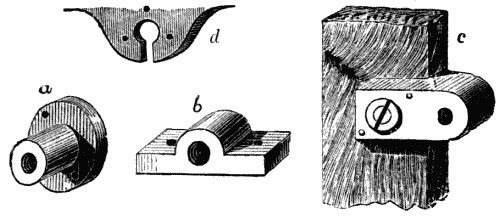
\includegraphics[width=\textwidth]{images/fig38.png}
\label{fig38}
\end{figure}

Fig.~\ref{fig39} is a front elevation of those Mexico clocks, showing
as much as can be shown at one view without confusion,
and representing the wheels only as circles for the same
reason. They have $1$~sec.\ compensated pendulums with
bobs of nearly $1\frac14$~cwt.; where there is room, of course it
would be better to use $1\frac12$ or $1\frac34$~sec.\ pendulums. They
are calculated to strike the hour on a bell of $4$ or $5$~cwt.\ with
quarters in proportion, and will drive four $6$~ft.\ dials very
well. The whole length of a quarter clock on this pattern
is only $30$~inches, and for one without the quarters $21$~inches.
The flies may require rather more, according to the size of
the hammers. One fly\index{Turret clocks!position of fly} may go behind the other if necessary.
Those who build clock-towers should remember that
%-----File: 208.png-----------------------------------------------
%-----Folio: 193--------------------------------------------------
\index{Turret clocks!larger ones}\index{Turret clocks!smaller ones}%couldn't find ref
there must be room for a man to stand and wind up the
clock besides. The hole in the upright bar where the pallets
are shown, is only in the back bar, which is widened out for
\begin{sidewaysfigure}[p]
\centering\index{Beckett, Sir E.!general plans for turret clocks}
\caption{\sc Four-wheeled Train Clock}
\label{fig39}
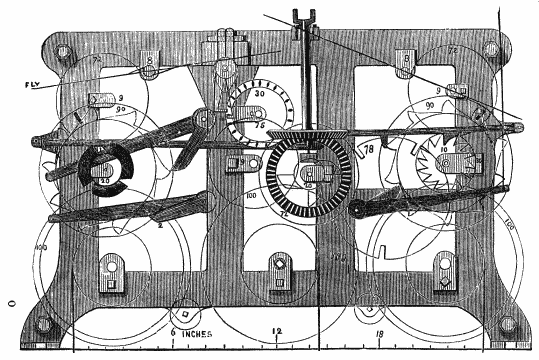
\includegraphics[width=\textwidth]{images/fig39.png}
\end{sidewaysfigure}
%-----File: 209.png-----------------------------------------------
%-----Folio: 194--------------------------------------------------
it, and the two lumps which form the pendulum cock are
cast on the back. The cross bar which carries the locking
plate $78$ is only wanted on the front frame, and is omitted
on the back one, as it would interfere with taking out the
barrel. All the levers are so placed as to clear the ropes
when they have to be taken upwards. The small cam wheel
for lifting the locking lever of the striking part answers very
well: that of the quarters is in fact the locking plate itself.
If there are no quarters at the hour, the pinion of $20$ should
be $30$, and drive a separate locking wheel of $36$, which
will turn in $2$~hours, as $12$ cams are used in that time.

\subsection[Size of fly.]{Size of fly.}\markboth{LARGE FLIES BEST.}{LARGE FLIES BEST.}\label{subsec:Size_of_fly.}\index{Fly, striking!for turret clocks}---There is no more frequent mistake in turret
clocks than that of making the fly too small to preserve uniformity
of time in striking, and the defect is generally incurable
for want of room. When the fly of the hour striking part is
too small the velocity increases after the first few blows; and
with quarters on four bells especially, some blows come
quick and others slow, according as the heavy or the light
hammers are being raised. You must have a considerable
superfluity of force beyond what will just raise the hammers,
and the regulation of time must be done by the fly. I do
not however see my way to prescribing any rule for the size
in proportion to the weight of hammers or bells beyond this,
that each arm of the fly of any large church clock ought to
be fully $2$~ft.\ long; and for the very large bells which have
lately come into fashion again, the flies must be still longer.
Length is much more effective than width. There may be
from $4$ to $8$ turns for each blow or each quarter, according
to the size of the clock. At Westminster we could get no
uniformity of striking quarters with a fly going faster than
$4$ times to each chime; $6$ or $7$ is generally the best number.

When it is impossible to get room for flies of proper
length and size to equalise the time, something may be done
by using a three-armed fly, but that is by no means equal to
one with two arms of sufficient length.
%-----File: 210.png-----------------------------------------------
%-----Folio: 195--------------------------------------------------

I find it necessary to add, that the flies should on no
account be in front of the clock, for that involves the use of
a winder with a very long pipe to clear them, which is
harder to wind and strains the arbors. Fig.~\ref{fig47} will show how
to get plenty of room for them behind in clocks of almost
any size. In very large ones, such as Westminster, a
vertical rod may be carried up and the flies put quite away
at the top of the room. I have seen it done also in much
smaller clocks where there was no room otherwise for the flies.

\section{LARGE CLOCKS WITH QUARTERS.}\label{sec:LARGE_CLOCKS_WITH_QUARTERS.}\markboth{LARGE QUARTER CLOCKS.}{LARGE QUARTER CLOCKS.}

Fig.~\ref{fig40} (\textit{t.~o.}) is a front view of a larger clock than those
previously described, substantially according to the plan
which I settled for old Mr.~Dent's factory many years ago,
whereby we reduced the cost of large quarter clocks to little
more than a quarter of what it used to be, and at the same
time greatly increased both their accuracy and strength.
This only shows two quarter hammers for simplicity. Indeed
four could not be shown in an elevation, as the levers must
then all be on one axis or pin, and the cams come irregularly,
as will be explained under quarter chimes. As Fig.~\ref{fig37} was
of an eight-day clock, to which a quarter part might be
added much like the hour part, this is of larger clocks, with
heavy bells, and winding up the striking parts every day or
two days, according to the available fall. It is impossible to
strike heavy bells properly with an eight-day clock unless it
has a very unusual fall, and even then it would want very
inconveniently long barrels, and the old-fashioned clocks never
did strike properly.

The hour great wheel \hyperlink{fig40}{here} has only $10$ cams, which I
consider the best number for the arcs that have to be described
by the cams and the hammer-tails or levers, when we are free
to use any number, which we cannot in eight-day clocks.
Therefore this requires only $16$ turns of the barrel for $24$
%-----File: 211.png---------------------------------------------
%-----Folio: 196------------------------------------------------
\begin{sidewaysfigure}[p]
\centering\index{Beckett, Sir E.!general plans for turret clocks}
\hypertarget{fig40}{\caption{\sc Large Quarter Clock}}\label{fig40}
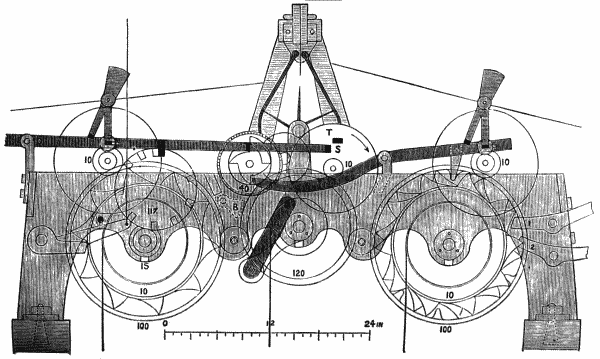
\includegraphics[width=\textwidth]{images/fig40.png}
\end{sidewaysfigure}
%-----File: 212.png---------------------------------------------
%-----Folio: 197------------------------------------------------
hours, or $156$ blows, and $2$ or $3$ more for a few extra hours;
or say $35$ or $36$ turns for winding every two days; and
therefore quite short barrels will do, with wire ropes as much
as $\frac 14$~in.\ thick, which are enough for all but very large
clocks beyond the ordinary patterns.

The going part is always made to go a week, or rather $8$
days and a fraction, to provide for the forgetting of a day.

\index{Large turret clocks}\markboth{LARGE TURRET CLOCK.}{LARGE TURRET CLOCK.}It is impossible to give any rule for the size of the great
wheels, as it clearly ought to depend on the work they have
to do. For bells from about $30$~cwt.\ to $53$, a common range
for the tenors of large peals, an $18$-in.\ great striking wheel is
the best pattern to keep, as it is inconvenient to use many.
A $24$-in.\ wheel with only $10$ cams of proper size and strength
will do very well for bells up to $5$ or $6$~tons, or even $10$~tons,
if the teeth and cams are wide enough. The great going
wheel may be from $13$ up to $16$~inches for any four dials
from $7$ up to $12$~feet, and there are very few larger. The
other wheels may be in proportion. The scape-wheel legs
should be from $5$ to $6$~inches long, and you must allow
plenty of room for a long fly, not less than $9$ or $10$~inches,
especially for large dials, which should have a considerable
superfluity of force, to drive the hands in all weathers. For
that reason the scape-wheel arbor is put on a higher cock
than before. The pendulum is carried in the same way by
the frame. If it is a very large one it is well to put one or
two brackets or strutts from the wall to the back part of the
frame near the pendulum, but that is not necessary generally,
as this kind of frame for $18$-in.\ great wheels is only $5$~ft.\ $6$~in.\ long,
and forms a kind of arch when its feet are firmly bolted
to the corbels, which I need not say should be a great deal
deeper than there was room to show in \hyperlink{fig40}{this drawing}. If they
are iron brackets they should be built into the wall and wide
at the top also, to prevent any risk of sideway motion under
the swing of the pendulum.

For\label{nocams} $10$ cams the great wheel had better have \index{Wheels, numbers of teeth}$100$ teeth,
%-----File: 213.png---------------------------------------------
%-----Folio: 198------------------------------------------------
and the pinion $10$; or $120$ and $12$ of course run rather easier,
which pinion will evidently go once round for each blow.
But if you want the clock to go $4$~days without winding and
to have only one hammer, $16$ cams will be better, and $192$
teeth in the great wheel, driving a pinion of $12$ \label{twothirds}two-thirds
round for each blow. And then you may make the cam wheel
on that pinion with $2$ hollows in it one-third and two-thirds
of the circumference apart, and they will always come
right, because the number of the hours is odd and even
alternately, if it is put in the right position; which you
will find more easily by trial than by explanation here. But
this would not do when half-hours are struck by the hour
part, for two odds then often come together, such as $3$ and $1$,
$5$ and $1$, \&c. The general calculation for all numbers is
this. Let $p$ be the leaves of the pinion, which must be a
multiple of $3$ if you are to use that method; $n$ the teeth of
the great wheel, and $m$ the cams. Then $\frac23 p$ must $= \frac{n}{m}$ or
$n = \frac23mp$: $p$ must be taken as $12$ for this purpose, and
$\therefore n = 8m$. If $p$ has $10$ leaves and is only to go once
round, $n$ must evidently $= 10 m$. It is not convenient to have
two large hammers with a ringing peal, as it is difficult to
get room for them in the frame, though it is easy enough for
stationary clock bells. But it is unnecessary to consider all
that if the clock winds up every day or two, which is always
best for large ones. A few cocks and bushes are omitted in
the drawing to avoid confusion.

In other respects this striking\index{Turret clocks!striking part} part is the same as in fig.~\ref{fig37}.
But I now show the plan for letting off the \markboth{LARGE QUARTER CLOCK.}{DISCHARGE OF STRIKING PARTS.}striking of
the hours more exactly than can be done by the slow motion
of the hour wheel and its snail, especially as it is a sort of
outrider to the train. This was first done in the Westminster
clock, but the plan now described for the first time was not
expedient there on account of the great size and weight of
%-----File: 214.png---------------------------------------------
%-----Folio: 199------------------------------------------------
the discharging\label{disch} levers. \hyperlink{fig40}{Here} you see that the long lever or
detent $\mathrm{DS}$ is carried over to the second wheel of the going
train, which has a square pin $\mathrm{T}$ on one of its spokes; and
there is another square pin $\mathrm{S}$ on the detent, now shown
below the other, the clock having just struck. But at some
minutes before striking $\mathrm{S}$ gets raised above the circle in which
$\mathrm{T}$ moves, which can be done, because at that time $\mathrm{T}$ is out of
the way. Just before the detent is going to drop off the snail
$\mathrm{T}$ has come under $\mathrm{J}$, and $\mathrm{J}$ cannot fall again till $\mathrm{T}$ slips from
under it, which will take place with perfect \index{Striking clocks!accuracy of discharge}accuracy at the
last beat of the pendulum for the hour, as the motion is large
enough to be visible, and a very little way off the scape-wheel.
This is inconsistent with altering the hands less than $15$ or $20$
minutes, except by running the clock, as you easily can with
a gravity escapement. In the Lincoln\index{Lincoln Minster clock} Minster clock Mr.~Potts\index{Potts, maker of Lincoln Minster clock and others}
provided in this way for the quarters also, as did
Messrs.~Smith at St.~Paul's and Beverley\index{Beverley!clock}, which however
are not of so much consequence as the first blow of the
hour. The second wheel must in that case turn in $15$
minutes; but without the quarters it may be either $20$ or $15$.
The pins $\mathrm{S}$ and $\mathrm{T}$ should be so placed and shaped that the
pressure may not tend to stop the wheel. (See also p.~\pageref{addenda_start}\label{199add}.)

As I have already shown the maintaining\index{Maintaining powers of clocks or going barrels!Westminster clock plan} power which is
best for clocks not requiring an auxiliary winding wheel, I
show here the one which is best for those that do; though
the other, of which a piece is shown at $\mathrm{B}$, may be used for
them. This is the one that I designed for the Westminster
clock, and the principle of it will be described there. The
winding pinion and the bars which carry it, the front one
fixed and the back one hanging from the arbor, are out of the
vertical, because the action of gravity is wanted to make the
pinion and back bar which carries it fall on to a fixed stop,
when the winding is done, or suspended for a short time.
The back bar also carries the click which takes into ratchet
teeth cast on the back of the great wheel. It might go into
%-----File: 215.png---------------------------------------------
%-----Folio: 200------------------------------------------------
the other teeth, but for the risk of catching only on their tops
and slipping, so that ratchet teeth are safer, and practically
cost nothing when once the patterns are made to cast from.

The arrangement of the quarter part for $4$ bells is practically
the same as for $2$, except that all the levers must be on one
steel pin, which should be screwed tight at its ends to help
to keep it stiff. Either for $2$ hammers or for $4$, the best way
is to cast one set of cams on one side of the great wheel and
another on the other, at the proper distances to make the
interval between successive chimes at least twice as great as
between the blows in each chime. For $4$ bells two other
sets of cam rings may be cast in one, and all bolted together.
Some clockmakers prefer an independent cam barrel driven
by the great wheel, to which there is no objection except the
extra friction, which I once found to make the difference of
requiring an auxiliary winding-wheel. When steel cams are
used they are all bolted to a wide ring or barrel cast with
or bolted to the great wheel, the nuts being inside it. I shall
have more to say about cams afterwards. Four quarter
hammer-tails cannot well be turned inwards as the hour one
can, in the form which makes the pressure on the arbor only
the difference instead of the sum of the two forces on the
lever. But they can have their wires in the middle, instead
of their fulcrum or arbor being there, as you see in the
Westminster clock, and in that way the friction on their arbor
is reduced to a minimum, the wires being put as near the
cams as possible. (See also p.~\pageref{add200}\label{200add})

Two \markboth{WAY OF FIXING TWO QUARTER LEVERS.}{WAY OF FIXING TWO QUARTER LEVERS.}quarter hammers---or two alternate hour hammers---can
also be placed as in this fig.~\ref{fig41}, which I designed long
ago with the same object of keeping the power and the work
on the same side of the arbor, and many large clocks were so
made at Dent's factory. It involves cams on both sides of
the great wheel, which are as easily cast as on one side. The
rope also should always pull on the same side of the barrel as
the cams, in order that the pressure on the great arbor may
%-----File: 216.png---------------------------------------------
%-----Folio: 201------------------------------------------------
\index{Quarter chimes!on two bells}be the difference instead of the sum of the weight and its
work, and consequently the friction much less. You may
fancy that these frictions of pivots, and of teeth when the
cams are not on the great wheel, cannot come to much compared
with a great striking weight, or a hammer of many
pounds weight raised $9$~in., or about $6$ vertically, $156$ times a
day; but you will find very few clocks in which the weight
$\times$ its daily fall is not more than twice or even three times
its theoretical `duty,' or the hammer $\times~78$~ft., which excess
is all due to these various frictions.

\begin{figure}[htbp]
\centering
\caption{\sc Two-quarter Hammer}
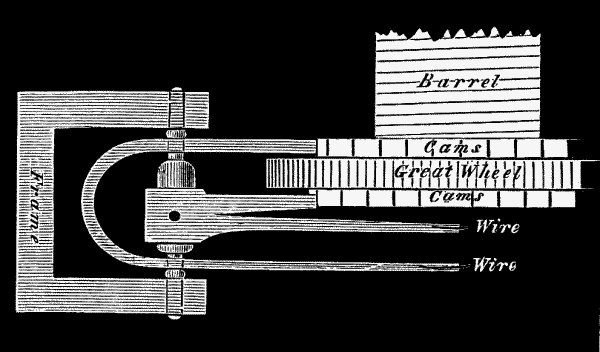
\includegraphics[width=\textwidth]{images/fig41.png}
\label{fig41}
\end{figure}

If no quarters are struck at the hour it is better to have $12$
cams, the locking-plate being on the great wheel arbor, so
that they will turn in $2$~hours. In that case the pinion may
as well be of $12$, driven by the great wheel of $96$, and
therefore turning $\frac23$ round for each quarter chime as before
described for hours in some cases.

Lifting the hammer by pins on the striking wheel, as in
house clocks, is totally wrong in large ones, and it is nearly
discontinued. The pins necessarily begin to act a good way
from the end of the lever, and therefore at the greatest disadvantage
%-----File: 217.png---------------------------------------------
%-----Folio: 202------------------------------------------------
as to leverage, and that at the very time when
the hammer is rising most vertically (in the usual way of
hanging) and requires the most force to lift it. The lifting
should be done by cams, which begin to act on the end of
the lever, and are properly shaped to act with the least
possible friction throughout, as I shall explain under the
\textit{Teeth of Wheels}. Pins with rollers on them are of very little
use, and do not obviate these objections, and are weaker than
fixed pins: they are nearly if not quite abandoned.

\subsection[Cambridge and Westminster chimes.]{Cambridge and Westminster chimes.}\markboth{QUARTER CHIMES ON FOUR BELLS.}{CAMBRIDGE AND WESTMINSTER CHIMES.}\label{subsec:Cambridge_and_Westminster_chimes.}\index{Cambridge and Westminster chimes}\index{Chimes (quarter)!Cambridge and Westminster}---Considering
the thousands of men who had listened for 3 or 4 years
together to the famous St.~Mary's chimes at Cambridge,
during three quarters of a century, it is odd that no one
ever thought of copying them in any other public clock.
The last but one Lord Lansdowne tried it, but his clockmaker
Mr.~Vulliamy\index{Vulliamy, Mr.} made the mistake of ordering and hanging
the bells of four successive notes before writing to ask me
about them; whereas they ought to be such notes as E, D,
C, G; or the fourth bell must be a musical `fourth' below
the third: bells are always counted from the highest note
or smallest bell. At the Royal Exchange\index{Chimes (quarter)!Royal Exchange}\index{Exchange, Royal!chimes}, in 1845, they did
get so far as to adopt the Cambridge notes; but the Gresham
professor of music thought he could improve upon the tunes,
and spoilt them. I have been told by a Cambridge man of
the last century, that they were invented by the well-known
Dr.~Crotch in 1780, from an air of Handel's, who has
generally had the credit of inventing them, and perhaps
deserves it.

\subsection[Doncaster quarters.]{Doncaster quarters.}\markboth{QUARTER CHIMES ON FOUR BELLS.}{DONCASTER QUARTERS.}\label{subsec:Doncaster_quarters.}\index{Doncaster!quarter chimes|(}\index{Chimes (quarter)!Doncaster and Scarborough}---For some time after I thought of
introducing them at Westminster, it was assumed that the
hour bell must be an octave below the third quarter, and
that they were therefore impossible with a peal of only $8$
bells, if the quarters were to be struck at the hour. Moreover
playing $10$ chimes in every hour, requires nearly twice
as much power in the clock as playing $6$, which is sometimes
%-----File: 218.png---------------------------------------------
%-----Folio: 203------------------------------------------------
a consideration when there is not much fall for the weights,
and it makes a little difference in the cost. Again, if you
look at the Cambridge chimes (p.~\pageref{camchimes}) you see that the blow
on the lowest quarter bell (called 6), is repeated too quickly
in one place for a heavy hammer to be relifted immediately;
and accordingly in all very large clocks it is necessary, and
it is always desirable, to have two of those hammers, lifted
alternately. Avoiding it by a separate barrel, driven by the
great wheel, is a much worse plan. For all these reasons, in
a few church clocks, made before 1860, I adopted the plan
of omitting the quarters at the hour; but I should not do
so again with these quarters, because the hour chime is the
best of them all, though \textit{ding dong}, or any other mere
repetition quarters, are neither useful nor pleasing at the
hour. I also made a slight alteration in the third quarter in
those clocks, to avoid the quick relifting of the largest
hammer, and it sounds very nearly as well as the Cambridge
one. The quarter bells are therefore, $2$, $3$, $4$, $7$, of a peal
of $8$ at Doncaster and Scarborough parish churches, and the
cathedral at Fredericton, where the three-legged gravity
escapement was also first used.\index{Doncaster!quarter chimes|)}

\subsection[Worcester and Chester Cathedral quarters.]{Worcester and Chester Cathedral\index{Chester cathedral chimes}\index{Chimes (quarter)!Chester and Worcester cathedrals}.}\markboth{QUARTER CHIMES.}{QUARTERS ON FOUR BELLS.}\label{subsec:Worcester_and_Chester_Cathedral_quarters.}---But
after a time I came to the conclusion, and other people have
gradually adopted it, that it is not at all necessary to have
the third quarter bell an octave above the hour bell, and
that the ear is quite satisfied if the fourth bell is two notes,
or even one, above the hour, because the interval of time
between the quarters and the hour ought to be from $6$ to $10$~seconds
with large bells. Accordingly in the great peal at
Worcester\index{Worcester cathedral!chimes, peculiar}, the Rev.~E.~Cattley\index{Cattley, Rev.~R.!Worcester chimes}, the author of it, and I,
as the designer of the clock and bells, agreed to take advantage
of the tenor of the peal for the fourth quarter bell,
though it is only $1 \frac12$ notes above the great single hour
bell of $4 \frac12$~tons; and thereby we got far more powerful
quarters than if we had kept them $2$ notes higher. At
%-----File: 219.png------------------------------------------------
%-----Folio: 204---------------------------------------------------
Chester Cathedral, and St.~Chad's, Headingley\index{Chimes (quarter)!Headingley}\index{Headingley, St.~Chad's chimes and peal}, near Leeds
and some other places, the 4th quarter bell is only one note
below the tenor, as at Doncaster, though they are the full
Cambridge quarters; and that is the plan which I now
always recommend when there are $8$ bells, or even $6$, with
an extra one added above for the first quarter. At Ossington
Church, having only a small peal of $6$, I recommended
to my namesake the late Speaker, a lower bell (out of the
peal) for the hours; and the same at S.~Shields lately.

The \hyperlink{camchimes}{following} are these several arrangements, which are
suitable for any key, and therefore I have indicated them by
the bells in a peal of $6$, which these quarters require, leaving
the hour to be any note below the lowest quarter bell.

\begin{table}[!hbtp]
\centering\index{Cambridge and Westminster chimes}\index{Cambridge and Westminster chimes}\index{Chimes (quarter)!Cambridge and Westminster}\index{Chimes (quarter)!Doncaster and Scarborough}\index{Chimes (quarter)!Royal Exchange}\index{Exchange, Royal!chimes}\label{camchimes}\hypertarget{camchimes}{}\index{Table!various quarter-chimes}
\begin{tabular}{r@{\,}c@{\,}r|l@{\,}l|l@{\,}c@{\,}l@{\,}l}
\multicolumn{3}{c|}{Cambridge and}  &
\multicolumn{2}{c|}{Doncaster and}  &
\multicolumn{4}{c}{Royal Exchange.}   \\[-0.5ex]
\multicolumn{3}{c|}{Westminster.}   &
\multicolumn{2}{c|}{Scarborough.}      \\[1ex]
\multirow{2}{*}{2nd $\Big\{$}  &3126  &\multirow{4}{*}{$\left.\rule{0pt}{5.5ex}\right\}$ 4th} &
1st                            &1236  &1st                                                    & 3126                          &\multirow{2}{*}{$\Big\}$ 2nd} &\multirow{4}{*}{$\left.\rule{0pt}{5.5ex}\right\}$ 4th}\\
                               &3213  &                                                       &\multirow{2}{*}{2nd $\Big\{$}  & 3126                         &\multirow{3}{*}{3rd $\Bigg\{$}                           &6213 & &\\
\multirow{3}{*}{3rd $\Bigg\{$} &1326  &                                                       &                               &3213                          &                                                         &1326 & &\\
                               &6213  &                                                       &\multirow{3}{*}{3rd $\Bigg\{$} &2613                          &                                                         &3213 & &\\
                               &1236  &1st                                                    &                               &6213                          &                                                         &     & &\\
\end{tabular}
\end{table}

I call the bells $1$, $2$, $3$, $6$, in all cases for more easy
comparison, though they would be of various numbers
according to the peal they belong to, on account of the
numbers being always reckoned from the smallest, in the
order in which they ring. Indeed a peal of $6$ could not have
these chimes at all without an odd bell, either above as at
Headingley, or below as at Ossington.

You see from the table that the Cambridge chimes are
repeated twice in the hour, and therefore the cams may be
fixed on a barrel\label{barrel} which turns in any multiple of the $5$ chimes
in that table. In some clocks the $5$ sets of cams alone are
put on a barrel driven by the great wheel, but with much
more friction than in other clocks that I know with bells
%-----File: 220.png-----------------------------------------------
%-----Folio: 205--------------------------------------------------
of about the same weight; one, with this second barrel,
required a double multiplying power to wind it up, while
another, with the cams for an hour on the great wheel itself,
winds quite easily with a single pinion. At Westminster, as
you may see in the frontispiece, there are $3$ sets of cams, or
what may be called an hour and a half's chimes, on the
great wheel, \textit{i.e.}\ on a wide barrel attached to it, because it
happened to be convenient with the great fall we have there.
The cams may be cast in separate rings of cast steel, but it
is better to have smooth-faced steel cams screwed firmly to
a plain barrel, as they are at Westminster, and in all the best
very large clocks now.

The interval\label{interval}\index{Chimes (quarter)!interval between each quarter} between each chime (\textit{i.e.}\ between the chimes
of each quarter) requires some attention. At Cambridge it
is $3$ times the interval between the blows of each chime. That
appears to me decidedly too slow, and at Westminster, Doncaster,
\&c., I made the interval only two spaces instead of
three. That again is perhaps rather too quick, and at
Worcester, and all the subsequent large clocks for which I
have given designs or specifications, there are $2\frac12$ spaces,
which sound the best of all. The barrel, or each portion of
it which contains the $5$ chimes, must then be divided into $55$
spaces, of which each blow occupies $2$, and the intervals
between the chimes $5$ spaces.

When there are two hammers for the 4th bell, as there
always should be, those cams may, and should be, made
longer than the others, as there is then ample room for it;
which diminishes the pressure on them, and makes it more
continuous, and so tends to equalise the time. This is
important, because the 4th quarter bell is much the heaviest,
and there is the least interval between its blows.

In\markboth{LIFTING OFF HAMMERS.}{LIFTING OFF HAMMERS.} all quarter clocks, striking on a peal of ringing bells, provision
should be made for lifting off\index{Hammers, clock!lifting off}\label{lift} the hammers, or they are
almost certain to be broken when the bells are rung, and
perhaps the bells cracked besides. This is easily done by a
%-----File: 221.png-----------------------------------------------
%-----Folio: 206--------------------------------------------------
lever; or, when the hammers are very heavy, it is better
done, as Mr.~Cattley\index{Cattley, Rev.~R.!lifting off hammers}\index{Turret clocks!lifting off hammers for ringing} arranged at Worcester\index{Worcester cathedral!clock}, by an eccentric
brought down over all the levers just where they come out
of the clock. The hammers must not only be lifted off the
bells, but so high that the cams do not lift them at all, or all
the wires will soon be broken by the jerks. And as the
clock is thus relieved of its work, it is better also to make
the turning of the eccentric, or pulling down the lever, let
down a wooden brake on the fly arbor, to help the fly to
stop the velocity and diminish the blow on the stops.

\subsection[Quarters on two bells.]{Quarters on two bells.}\markboth{QUARTERS ON TWO BELLS.}{QUARTERS ON TWO BELLS.}\label{subsec:Quarters_on_two_bells.}\index{Quarter chimes!on two bells}\index{Time of striking (quarters)}---I have little more to say about
turret clocks with these than I said about house clocks at
p.~\pageref{quart}. The bells must be at the musical interval called a
fourth, and the higher of the two should be an octave higher
than the hour bell if there are quarters at the hour; though
that is not so material, and they may be the 1st and 4th of
a peal of $6$, or even $5$, or the 4th and 7th of a peal of $8$,
because there should be a longish interval of time between
the quarters and the hour, which saves the ear from being
offended with the want of the proper musical interval. The
old York Minster\index{Chimes (quarter)!peculiar, on two bells at York Minster}\index{York Minster!quarter chimes, peculiar} quarters, and a few others, were at the
interval of a fifth (which in music, though not in arithmetic,
is larger than a fourth), but they do not sound so well.

\subsection[Time of striking.]{Time of striking.}\markboth{PRECISION OF STRIKING HOUR.}{PRECISION OF STRIKING HOUR.}\label{subsec:Time_of_striking.}\index{Striking clocks!accuracy of discharge}---The quarters are generally made to
let off the hour, as described at p.~\pageref{hourstrike}. But where accuracy
of time of striking is required, this plan is insufficient; for
it makes the first blow of the hour depend on the time both
of letting off, and of striking the quarters, both of which
may easily vary several seconds. It is therefore essential
to accuracy that the hour-striking should be let off by an
independent\index{Quarter chimes!should be independent of hour in large clocks} snail of its own, exactly at the hour, with the
quarters let off the requisite number of seconds before the
hour; though the other three quarters may be allowed to
strike at their proper times. Even this is not sufficient where
extreme accuracy is required, as I have already explained.
%-----File: 222.png-----------------------------------------------
%-----Folio: 207--------------------------------------------------
The hammer should also be left `on the lift,' or nearly ready
to fall; which is in other respects also a good thing in a very
large clock, because it relieves the wheels and the stopping
pieces from a heavy pressure, and throws it all on the cams
and hammer work, which must in any case be strong enough
to bear it. In this case it is necessary to put a small click
somewhere, to act on a pin in the fly arbor to prevent the
train from running back when you wind up the clock:
indeed it is as well to put one always, as the winding always
tends to drive the train back. Where there is no special
provision for accurate striking, as above, care must be taken
to make the discharging snail large, and its corners
sharp and hardened, and those of the discharging lever or
lifting piece also. See also p.~\pageref{disch}.

\subsection[Chime tunes.]{Chime tunes.}\markboth{CHIME TUNES.}{CHIME TUNES.}\label{subsec:Chime_tunes.}\index{Chime-tunes}\index{Tunes, chime}---There has been a considerable revival of
the old fashion of having tunes played on bells by machinery
for a few minutes at certain hours of the day. The old
machinery for this purpose was extremely simple, consisting
of a large barrel $2$ or $3$~feet in diameter, generally made of
wood, with strong iron pins screwed into it like a huge musical
box barrel, and pulling down levers which lifted hammers
on the bells like a common striking part. If there were
several tunes on the barrel, either that or the bed of levers
had an endway motion, shifting at the end of each tune, or
shifted once a day by the clock. The Royal Exchange\index{Exchange, Royal!chimes}
chimes are of this kind, only the barrel is of cast iron, with
a vast number of holes in it, in which pins or short cams
are screwed to play any tunes that the bells admit of.

Some new ones of the old kind have lately been put up in
St.~Albans\index{Chimes (quarter)!St.~Alban's cathedral}\index{St.~Alban's cathedral chimes} Cathedral by Mr.~Godman, a clockmaker there
whom I have mentioned before, entirely from his own design.
The barrel is $7$~ft.\ long, of wood on iron rings, and the levers
are worked by cams of `phosphor bronze' screwed on, for $8$
tunes on $8$ bells, which I think are quite tunes enough, and
more than were generally used in old times. The tunes shift
%-----File: 223.png-----------------------------------------------
%-----Folio: 208--------------------------------------------------
themselves. The Westminster quarters are also put there on
the same plan and in connection with the chimes in a room
above the clock. Notwithstanding the superiority of those I
am going to describe next when constantly looked after by
a competent person, which they require, and which of course
costs money, I have returned to the opinion that for ordinary
churches, where there are seldom any funds to spare,
the old-fashioned chimes are the best.

The chimes in some foreign churches\index{Foreign!churches, chimes in some}\index{Tunes, chime!on church bells} are played by hand,
I understand, without anything that can be called machinery.
The hammers, being light, are easily lifted a little by a man
playing on keys like a piano, only with his fist instead of his
fingers. I have seen tunes played on church bells here with
even less machinery than that. They just tie the bell-ropes
to the clappers, and the lower ends to rings on a board
screwed down to the belfry floor, bringing the clappers so
near to the bells that a slight pull will make them strike.
The man `operates' them (in American grammar) by pulling
some of the ropes with his hands and pushing others with
his arms, and so manages to play a feeble sort of tune.

\section{NEW CHIME MACHINERY.}\label{sec:NEW_CHIME_MACHINERY.}

The new kind just now referred to were introduced by
Gillett and Bland\index{Chime-tunes!improvements!by Gillett and Bland}\index{Gillett and Bland's!chime machinery|(} of Croydon, and by Lund and Blockley of
Pall Mall, both of whom bought some patent rights of an
inventor named Imhoff, and have both made improvements
of their own. The principle of the invention consists in
this, that the hammers are raised by a long barrel full of
cams which have nothing to do with dropping them, but
are continually at work raising any levers that happen to be
down. The levers are then caught and held by triggers,
which are let off by quite small pins on a wooden barrel just
like that of a common grind-organ. The barrel can also be
taken out and changed, besides each barrel holding several
tunes which change themselves by an endway motion. This
%-----File: 224.png-----------------------------------------------
%-----Folio: 209--------------------------------------------------
\label{folio_209}figure shows Gillett and Bland's mode of lifting. Each lever
has a jointed beak which is lifted by one of the $7$ cams on
the barrel belonging to that lever; and when it has been
caught by the trigger
at the other end the
cam slips away, and the
beak drops, so as to
clear the cam next below,
and gets caught
again by the next to
that, because it falls
on to a block which
stretches out the beak.
This gives a greater lift
for a given number of
cams, and so allows
more cams to be put in
the barrel and more
lifting to be done with
a given velocity.

\begin{figure}[htbp]
\centering
\caption{\sc New Construction for Chime Tunes}
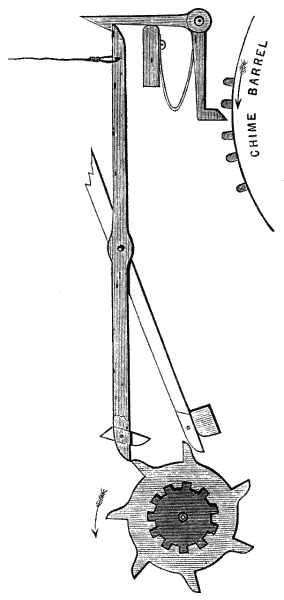
\includegraphics[height=0.7\textheight]{images/fig42.png}
\label{fig42}
\end{figure}

Lund and Blockley's\index{Chime-tunes!improvements!by Lund and Blockley}\index{Lund \& Blockley's!chime machinery}
lifting barrel has only
$4$ cams, and they lift
from $90^\circ$ before the
vertical up to their
highest position, by
means of a hinged
piece dropped from
each lever. They also
strike the Westminster
quarters by means  of
the same set of pins as
the tunes: which  I
must say I disapprove of altogether compared with a proper
quarter-striking part. I have seen an otherwise very satisfactory
%-----File: 225.png------------------------------------------------
%-----Folio: 210---------------------------------------------------
large clock of theirs, with chimes on a peal of $16$
large bells for the Bombay University; and some smaller
ones. Gillett and Bland's\index{Gillett and Bland's!chime machinery|)} principal chimes are at Worcester
Cathedral, Boston and Croydon Churches, Bradford and
Rochdale town-halls, and at Eaton Hall\index{Bells in peals!Boston and Eaton Hall}\index{Chime-tunes!Boston and Eaton Hall}\index{Eaton Hall bells}. The performance
of both kinds is more accurate and satisfactory than in the
old-fashioned machines; but, like most superior machines,
they require a great deal more care and consequent expense
than the old rough ones. No chiming machinery can bring
the full tone out of bells, especially the large ones: but this
is stronger in lifting as well as more exact in letting off than
the old kind. Every bell requires two hammers, and at
Worcester some of them have three, because of the quick
repetition in some of the tunes.

It is necessary to give one caution most strongly to
ambitious chime-cultivators. Avoid `chords,'\index{Chords in chime-tunes bad@`Chords' in chime-tunes bad} or two notes
sounded (professedly) at once. At Croydon they thought
they knew better, and a more horrible performance I never
heard from the rudest old-fashioned chime barrel of 200
years ago. I believe the chords have since been abolished.

Another caution is, not to attempt chimes on large and
small bells together\label{lsbad}\index{Bells in peals!large and small together, bad}. For some reason, which neither I nor
the bell-founders know, it is a fact well known that bells
below $4$ or $5$~cwt.\ cannot be made to sound homogeneous with
large ones. I shall have more to say of that in the chapter on
bells. They attempted it at Boston, and have got $42$ bells (including
the $8$ of the peal), some of only a few pounds weight
cast in Belgium, and chimes to play on them all together. I
and other people who went specially to hear them considered
them a failure. Even quarter chimes are never satisfactory
when large and small bells are mixed. The same result is
unpleasantly conspicuous at Eaton, though the bells there are
not so numerous, and were all cast in Belgium together.

\subsection[Clock hammers.]{Clock hammers.}\markboth{CLOCK HAMMERS.}{CLOCK HAMMERS.}\label{subsec:Clock_hammers.}\index{Hammers, clock}---Turret clocks generally strike on bells
of a different shape from the hemispherical house clock bells,
which do not answer beyond a very small size, as I shall
%-----File: 226.png--------------------------------------------
%-----Folio: 211-----------------------------------------------
explain more fully hereafter. Most people (except artists,
who always draw them wrong) are aware that the general
shape of church bells is that shown in figs.~\ref{fig43}, \ref{fig44}. The
clock hammer $\mathrm{CS}$ is always fixed\index{Hammers, clock!fixing}\markboth{FIXING OF HAMMER.}{FIXING OF HAMMER.} at right angles to the
swing of the bell, for two very obvious reasons: first, if the
bell was free to swing\index{Bell-hanging!for clocks} under the blow of the hammer, the
first blow of every hour would set it swinging a little, and
at every blow after that the bell would either be out of the
reach of the hammer altogether, or else jarring against it;
and another reason (if it is worth while to talk of other
reasons after this) is, that if the hammer was put in front of
the bell, all its machinery would have to be moved out of
the way before the bell could be rung at all.
\begin{figure}[htbp]
\centering\index{Hammers, clock!shape}
\caption{\sc Clock Hammer}
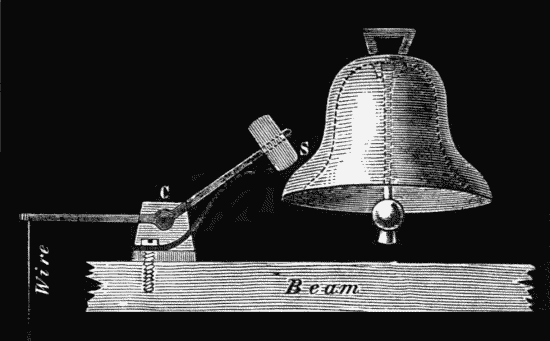
\includegraphics[width=\textwidth]{images/fig43.png}
\label{fig43}
\end{figure}

The hammers of large clocks also differ from small ones in
acting by gravity, as you see. But they equally require a
check spring, or some other contrivance to keep them from
jarring the bell. When a church bell is rung \textit{up, i.e.}, swinging
once round for each blow, and \textit{set} mouth upwards, the
clapper lies  on the bell, but not so heavily as a clock
%-----File: 227.png--------------------------------------------
%-----Folio: 212-----------------------------------------------
hammer would, because it stands at a higher angle. The
usual kind of hammer spring is shown in fig.~\ref{fig43}; and $sc$
in fig.~\ref{fig44} shows as much of the spring as there was room for.
\begin{figure}[htbp]\index{Bell-hanging!for clocks}
\centering
\caption{\sc Hammer Over Bell}
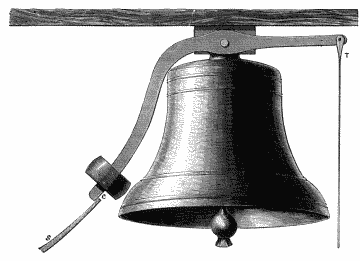
\includegraphics[width=\textwidth]{images/fig44.png}
\label{fig44}
\end{figure}
%-----File: 228.png--------------------------------------------
%-----Folio: 213-----------------------------------------------
The spring is sometimes made adjustable, by having long
holes for the screws to go through, so that you can bring it
farther from or nearer to the bell as may be required in
course of time. India-rubber buffers\index{Buffers for large hammers} under the hammer
shank are better in some positions, and have the advantage
of never breaking, and being easily replaced or altered in
thickness. I used them at Westminster.

I \markright{MODES OF HAMMER FIXING.}believe it is the fashion on the continent to fix the clock
hammers with their pivots above the bell, when it has not
to swing; and it has the advantage of securing a long
hammer shank, and therefore less angular motion for a given
lift, and moreover the effective weight of the hammer is not
so much lost in the lift as it is in the common position. But
on the other hand, with bells as tall as the foreign ones are,
the hammer shank stands much more vertically than in the
other way, and the rebound from the buffers or check spring
is greater, and a greater lift (obliquely) from the bell is
required to get the same momentum of the hammer; not
that that imposes more work upon the clock. At Westminster
we were obliged to adopt that plan, on account of
the construction of the tower and bell-frame, and there it
had this incidental advantage with regard to the great bell,
that we were enabled to get the hammer tail $\mathrm{T}$ directly over
the end of the lever in the clock, by setting the hammer
frame, or the pivots which carry it, a little out of the
cardinal position relatively to the tower, and so all cranking
was avoided and a vast quantity of friction saved.

\subsection[Cranks.]{Cranks.}\markboth{CRANKS.}{CRANKS.}\label{subsec:Cranks.}\index{Cranks, different forms of}---Nobody who has not tried it can have any
idea how much of the force of a clock is wasted by having to
lift the hammer through cranks. Where the hammers are
not very heavy, you may sometimes use what I shall call
\textit{couple-levers} (for a reason which any mathematician will
know), of the form in fig.~\ref{fig45}~$a$, instead of a pair of cranks;
but when the hammers are heavy, and the arbor of the lever
has to be long, I find it is impossible to avoid some elastic
%-----File: 229.png--------------------------------------------
%-----Folio: 214-----------------------------------------------
torsion in it, which wastes quite as much force as the
friction of a pair of cranks, and makes the hammers rise
with a tremble, which checks the force of the clock and
strains everything severely. For the same reason large
cranks should be made with a light connecting bar as in fig.~\ref{fig45}~$b$,
which increases the strength enormously and helps to
keep everything steady. The cranks and lever arms and
hammer shanks and tails should all be long. I know that
in modern towers, which are nearly always built too small
for properly hanging the bells, there is often great difficulty
in getting room for clock hammers and cranks at all; but
wherever there is room, the action will be easier and more
effective if all these arms are made long instead of short.

\begin{figure}[htbp]
\centering
\caption{\sc Forms of Cranks}
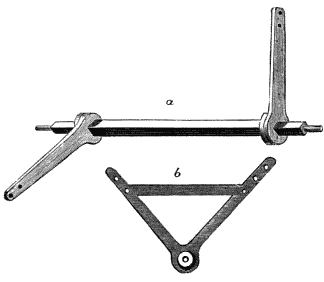
\includegraphics[width=324pt]{images/fig45.png}
\label{fig45}
\end{figure}

When the clock is above the bells, as in the Leeds town-hall,
and the Royal Exchange, it is a very common mistake
to put a tail to the hammer to pull down first, which of
%-----File: 230.png--------------------------------------------
%-----Folio: 215-----------------------------------------------
course involves the necessity for another to pull up again.
It ought to be done as I designed it at Leeds (if there is
room) by pulling up at once from a lever set inwards or on
the same side of the arbor as the hammer itself, unless it
happens from some local peculiarities that this would involve
as many cranks as the other way.

In several of the former editions I gave a design for
catching the hammer at its rebound without any buffer-spring;
but I have never heard of it being tried, and therefore
I do not repeat it, and have modified fig.~\ref{fig44} accordingly
to show a common buffer-spring.

\subsection[The weight of hammer]{The weight of hammer}\markboth{WEIGHT OF HAMMER.}{WEIGHT OF HAMMER.}\label{subsec:The_weight_of_hammer}\index{Hammers, clock!weight}\ and its lift can only be
determined by experiments. Different thicknesses and qualities
of bells require different hammers. I have generally
found that large bells whose diameter $=12 \times$ the thickness
of the \textit{sound-bow} or thickest part (which is the best
proportion) require hammers of about a $50$th of their weight
to bring out the full tone, and small bells require heavier
ones. The lift has to be less for small bells than for large:
the least that is effective in bells above $3$ or $4$~cwt.\ is $6$~in.\ (measured
obliquely in the direction of the motion), and
beyond $13$~in.\ we did not find any improvement in the sound
of either of the great Westminster bells. Generally they are
a great deal less either in weight or lift, and often in both,
and therefore you hardly ever hear a church bell sound so
loud under the clock striking as in ringing with the clapper.
Thinner bells, as the larger ones of peals usually are, do
not require such heavy hammers as thick ones; but it must
be remembered that no hammer arrangement will get as
good a sound out of a thin bell as a thick one, because it is
radically inferior both in quantity and quality of sound.
But I shall have more to say of that in the chapter on bells
hereafter. I only add a word of warning against a piece of
ignorance by which I remember a very fine old bell being
cracked in a few months---viz.\ making the clock hammer to
%-----File: 231.png--------------------------------------------
%-----Folio: 216-----------------------------------------------
strike it with a sharp edge instead of a flat or slightly rounded
face, as it ought to be.




\section{DIALS.}\label{sec:DIALS.}
\index{Construction of dials}\index{Dial work!of large clocks}\index{Dials!of public clocks}\index{Turret clocks!dials}\markboth{DIALS OF PUBLIC CLOCKS.}{DIALS OF PUBLIC CLOCKS.}

The striking of church clocks, and perhaps of public
clocks in general, is of more value than their dials, except in
places where the public congregate. Indeed dials a good
way above the eye are of no use for indicating the time
very accurately, on account of the parallax which affects the
minute hand, except when it is nearly vertical. Moreover
many church towers would be utterly defaced by dials;
And it is to be hoped that the splendid church of St.~Mary's,
Beverley, now that its fabric has been restored to a condition
worthy of its architecture, will not long retain those
abominable dials in the tower windows, which belong to the
age when the inside of the church was divided into private
boxes, in which people might eat their dinner or play at
cards without their neighbours or the clergyman knowing
anything about it.

But as dials must frequently be used, architects\index{Architects!their ignorance of requirements} might as
well condescend to learn something of their proper size, as
they profess to provide places for them, as they do for bells,
frequently in utter ignorance of what the provision ought to
be. Luckily there is such a simple rule for determining it
generally, which has now been long published, that they
have no excuse for doing it wrong. That rule is that the
diameter of the dial should not be less than a tenth of the
height of its centre from the ground. If you want to verify
this you have only to look at the dials of the Leeds Town
Hall, planned by an architect with the usual knowledge of
such things, $150$~feet high and only $11$ wide; and those of
the Bradford Town Hall\index{Bradford Town Hall tower and bells} are no better, but I do not know
the exact height; or that of St.~Pancras Church, $6\frac12$~feet
wide and about $100$~feet above the ground. The neighbouring
%-----File: 232.png--------------------------------------------
%-----Folio: 217-----------------------------------------------
railway station however has inside it a large dial
$15$~feet wide, at the height of $55$, looking down the
largest space under one roof without pillars in the world,
viz.\ $700$~feet long and $240$ wide (the length of the
transept of St.~Paul's Cathedral, and more than the length
of the nave of any cathedral except Norwich, Winchester,
and St.~Alban's, the longest of them all). The external
dial of that station is rather too small; but that, and some
others which comply with the above rule are given in this
list, which I have compiled from various sources.

\begin{table}[!hbtp]
\centering\label{largedial}\index{Table!sizes of public dials}
\begin{tabular}{lcrlr}
                           &\sc Dials. &\multicolumn{2}{c}{\sc Diameter.}&\sc Height.\\
                           &           &\ \ ft.      &in.\               &ft.\\
Mechlin                    &1          &40           &                   &about 300\\
Westminster                &4          &22           &6                  &180\\
St.~Paul's Cathedral       &2          &17           &                   &126\\
Shandon Church, Cork       &4          &16           &                   &\\
Pancras Station            &4          &12           &9                  &150\\
Scarborough old Church     &1          &12           &                   &on a hill\\
St.~James's, Piccadilly    &4          &10           &                   &\\
King's Cross Station       &4          &9            &                   &90\\
Bow Church                 &2          &9            &                   &70\\
Manchester Infirmary       &4          &9            &                   &80\\
Royal Exchange             &4          &9            &                   &90\\
St.~George's Church, Leeds &3          &8            &4                  &57\\
St.~Martin's in the Fields &4          &8            &                   &\\
Horse Guards               &2          &7            &5                  &\\
Marylebone Church          &3          &7            &                   &about 60\\
St.~Luke's, Chelsea        &4          &6            &10                 &72\\
The Queen's Stables        &6          &10           &                   &about 50
\end{tabular}
\end{table}

But if dials are sometimes too small, the opposite mistake
is often made, of figures\index{Dials!figures of}\index{Figures on dials useless, and proper size of}\markboth{SIZE OF FIGURES.}{SIZE OF FIGURES.} much too large, which is not a
compensation but an aggravation of the evil, for they practically
contract the size of the dial, in two ways; first by
%-----File: 233.png--------------------------------------------
%-----Folio: 218-----------------------------------------------
contracting the plain surface in the middle, over which the
hands are most distinctly seen; and secondly, the larger
the figures are, the more they run into each other and fill
up the space of the figure ring itself, and make it still more
difficult to distinguish the place of the minute hand. Ignorant
people fancy that you see what o'clock it is by reading
the figures; as if any single figure which you see in a clock
dial indicated the figure which you read off; except for the
hour hand, and the hour also is at once recognized by the
position of the hand. You see the long hand pointing to
VIII, and you say, `$20$~minutes to something.' Both for
the hours and the minutes everybody really judges from
the position of the hands, and $12$ large spots would do
as well or better than figures. I have several clocks without
any figures at all round the principal dial, only $12$ strong
marks; and I never found anybody who even observed the
fact that the figures were absent until it was pointed out
to him, or complained of the want of them then. I came to
the conclusion after various trials, that the figures and
minutes together ought not to occupy above one third of
the radius of the dial; the figures may be two thirds of that
one third; and the minutes from half to two thirds of the
remaining one ninth of the radius, with every fifth minute
strongly marked by a larger spot than the others. The
Westminster\index{Dials!of the Westminster clock} dials might have been clearer, considering their
great size. They are not of my design, except that I gave
the architect some suggestions for them, which are partly
followed and partly not followed. They are unnecessarily
confused with iron frame-work, and the clear space is unduly
contracted by some broad rings supposed to be ornamental.
The Midland Station dials are much better.

The only colours\index{Dials!colour and materials for|(} that seem to answer for dials and hands
are black or dark blue with gilt figures and hands, or some
very light coloured ground, such as white glass, with black
hands and figures. Good gilding will last fifteen or sixteen
%-----File: 234.png--------------------------------------------
%-----Folio: 219-----------------------------------------------
years, as at the Royal Exchange, in the worst London
atmosphere: bad gilding of course wants renewing much
oftener, and is probably the dearest. Gilt hands on a
light ground are a complete failure. The external counterpoises,
if there are any, should be painted the same colour
as the ground of the dial, except where they are very short
in proportion to the hands, as at Westminster, in which
case they cannot be mistaken at any distance for the hands
themselves, and practically increase their visible length.

Dials\index{Construction of dials}\label{dialmat}\markboth{CONSTRUCTION OF DIALS.}{CONSTRUCTION OF DIALS.} may be made of almost anything---stone, slate,
plaster, brick, iron, copper, and many old ones are of wood,
which however is the worst of all, as it always shows the
joints. In many cases the stone of the tower makes the
best dial. Generally it requires painting; but if it is such a
stone and in such a position that it will keep nearly white, it
will do very well with only the black figures and minutes
painted on it, and black hands, but by no means gilt ones.
Dials on brick work must of course be painted. It is quite
a mistake to suppose that a dial requires a very smooth
surface. Some of the most distinct I have ever seen are
painted on rather rough stone work; and brick will do as
well, either all flat, or with the figure circle a raised ring of
iron, or of any plaster that will stand. There are many
dials of cast iron; but I should never make more than the
figure ring of iron, unless there is a large hole in the wall
which wants covering; and even then it is generally better
to fill it with glass, which has all the effect of a dark ground
outside and is often convenient within. Slate makes a good
dial, but if it is not painted it becomes a pale grey colour.
I believe $6$~feet diameter is the largest size that can be got
in one piece, but the joints are almost invisible if well done.

Copper\index{Dials!colour and materials for|)} dials are the commonest of all, and up to a
moderate size, probably the cheapest, except of course
when the dial is simply painted on the wall. But they are
generally made in the very worst form that could be
%-----File: 235.png--------------------------------------------
%-----Folio: 220-----------------------------------------------
invented, viz., convex:\index{Dials!convex and concave} the effect of which is that the point
of the minute hand is thrown a long way off the dial, and
the parallax is so great that you cannot tell what it is
pointing at, except when it is nearly vertical, when seen
from below, as a public dial always is. One way to avoid
this is to countersink the middle, in which the short hand
travels, leaving the long hand to lie close to the raised figure
ring. I have lately seen some dials made of mosaic work,
like pavements, by Messrs.~Rust, of 16, Albert Embankment,
which look very well, and the price was not more than of
copper dials; and they can easily be made concave.

\subsection[Concave dials.]{Concave dials.}\markboth{CONVEX AND CONCAVE DIALS.}{CONVEX AND CONCAVE DIALS.}\label{subsec:Concave_dials.}\index{Beckett, Sir E.!concave dials}\index{Concave dials for large clocks}---It occurred to me some years ago that
all the convenience of the light copper dials might be got,
with even more closeness of pointing than in a flat one, and
with as much stiffness as the convexity gives, and with less
distortion of appearance, simply by making them concave
instead of convex. If you draw a vertical section of a
convex and a concave dial, and three lines of sight, from the
top, the bottom, and the middle of each, to a spectator in
the street, you will see at once that the convexity makes the
upper half appear much smaller than the lower, whereas in
the concave one the two halves appear even more alike in
size than in a flat dial; and the closeness of the hand pointing
is evident. There are now a good many of such dials, and
no one who has seen them can fail to perceive their superiority
to convex ones.

\subsection[Hands.]{Hands.}\markboth{CONSTRUCTION OF HANDS.}{CONSTRUCTION OF HANDS.}\label{subsec:Hands.}\index{Dials!hands of}\index{Hands of clocks and watches!for large clocks}---Large clock hands are so universally made of
copper that it is hardly worth while to notice any other
construction.\index{Hands of clocks and watches!proper construction and fixing}\index{Turret clocks!regulating and setting the hands} There is indeed---or was, a notable exception,
in Sir C.~Barry's famous gun-metal hands at Westminster\index{Barry, Sir C.!his Westminster clock hands},
which is not likely to be repeated. The hands of the clock
at old Doncaster church, which perished in the fire of 1853,
were of mahogany, and stood very well; but I should think
copper ones are lighter, even including the stalk or centre
piece. Where they are very large, say $5$ or $6$~feet long, the
%-----File: 236.png--------------------------------------------
%-----Folio: 221-----------------------------------------------
best form for them is that of the minute hands at Westminster,
viz.\ a tube of thin copper, whose section is two
segments of a circle, with a few diaphragms at intervals of
about $2$~feet to keep them stiff. The strength of this
construction is enormous, and it is also good for throwing off
snow, which sometimes accumulates on hands with broad
edges heavily enough to stop the clock. Smaller hands
may be made quite strong enough with a convex front and a
flat back, the section being an arc and its chord, or even as
a single flat piece of copper with the edges turned over
square. A mere rib or hollow bead raised along the middle
of a hand makes it strong enough for all ordinary sizes, but
it does not look well. `Galvanised' sheet-iron hands
have been tried, but the zinc peels off, and they must
be pronounced a failure. The minute hand should always
be straight, and plain, with a bluntish point. At the
broadest part, or near the dial centre, it should be about
a $13$th of its length, tapering to about half as much near
the point. The hour hand should be the same breadth,
ending just short of the figures in a broad piece called a
heart, of any shape you like.

There should always be some external counterpoises\index{Counterpoises for clock hands}\index{Hands of clocks and watches!counterpoises}\index{Turret clocks!counterpoises for the hands} to
large hands, both for wind and weight. They should not be
above $\frac13$ the length of the long hand, and should be broad,
but of a shape not to be confounded with the heart of the
hour hand. The advantage of counterpoising the hands to
some extent for the action of the wind is evident; and the
other use of an external counterpoise is to diminish the tendency
of the hand either to twist the arbor, or what is more
likely, to work itself loose and shake over from one side to
the other every time it passes the vertical, as Reid says the old
hand of St.~Paul's cathedral used to do, and as Sir C.~Barry's
heavy hands\index{Barry, Sir C.!his Westminster clock hands} did at Westminster to such an extent as to stop
the clock. The only way to prevent this shake is to fit the
hands on a tapered square or hexagon at the end of the
%-----File: 237.png--------------------------------------------
%-----Folio: 222-----------------------------------------------
arbor, and not a prismatic one. The latter may be called
engineers' fitting, and is perfectly right for many purposes
but perfectly wrong for this, for which the old clockmaker's
taper fitting alone will answer. It is found better not to
put the whole counterpoise for very long hands outside:
from one third to one half is quite enough, leaving the
remainder to be done by adjustable counterpoises inside,
which should be long rather than short, as they then do
the same work with less weight and friction on the arbor.

\subsection[Illuminated  dials.]{Illuminated  dials.}\markboth{ILLUMINATED  DIALS.}{ILLUMINATED  DIALS.}\label{subsec:Illuminated_dials.}\index{Dials!illuminated}\index{Illuminated dials}\index{Turret clocks!dials!illumination of}---Occasionally it is possible, as at
the Horse-Guards east dial, to illuminate a common white
dial by reflection from a lamp on a roof projecting below it.
This answers well enough for dials to be seen a short
distance only, in the few cases where it can be done.  Where
it cannot, the common way is to make the dial of glass, or
all of it except the figures and the rings to connect them
which form a solid framework of cast iron. The glass is
ground behind, or painted, or covered with muslin stuck to
it, and gas lamps are put behind it. But all these things
have such a bad appearance by day that the advantage of
illumination is dearly purchased at that cost. Now however
a white glass is made by Messrs.~Chance\index{Chance's glass for dials} of Birmingham,
and perhaps by other makers, which forms a very good
and always clean white dial by day (if left open for the rain
to wash its face) and a bright one by night: the hands and
figures must be black as with other white dials. It should
be $3$-$16$ths of an inch thick, or $22$~oz.\ to the square foot;
the middle of large dials has to be in two or three pieces,
which must be divided by bars not radial, or they  will
look like hands at night; and all but the figures and minutes
should be gilt.

The gas \label{gas}lamps of illuminated dials are generally kept
alight all day, turned down as low as they can be without
going out. They are usually tamed down in the morning
and up at night by a $24$~hour wheel in the clock, which has
%-----File: 238.png--------------------------------------------
%-----Folio: 223-----------------------------------------------
pins screwed into its rim and taken out again from time to
time by the man who takes care of the clock. So long as
any of the pins are in the position to hold up a weighted
lever connected with the gas cock, it is turned down, and
when the lever drops off it is turned up. In the Westminster
clock three fan-shaped pieces were prepared on a $24$~hour
arbor, which can be opened out to $18$~hours or contracted to
$6$, according to the length of illumination required; but it
was afterwards determined by the authorities to turn the gas
completely off and on by hand. There was a clock in the
Exhibition of 1851 with completely automatic or self-adjusting
machinery for turning gas off and on at the proper time
throughout the year; and Gillett and Bland did the same
in the Bradford Town Hall clock; but the tower is so small
and crowded with bell beams, that they were actually hot
by day, and I advised putting out the gas by day at least.
The machinery puts it quite out now. It cannot be done at
all accurately by any uniform automatic motion, because the
clock times of sunrise and sunset vary irregularly from the
equation of time (p.~\pageref{timetable}), and very slowly near the solstices,
but at other times from $12$ to $15$~minutes a week.

It is desirable to have a wall, if possible, behind illuminated
dials, instead of having them practically in the clock room;
partly because the wall may be made useful as a reflector,
and so save gas, and also because it protects the clock itself
both from the variations of heat and from the watery
vapour caused by burning the gas. Reflectors are a great
saving of light and of cost. It must be remembered also
that the counterpoises of the hands on glass dials must
neither be long ones outside, nor immediately behind the
glass inside, or they will cast a shadow and be confounded
with the hands at night. There should always be ventilation
over illuminated dials.

\subsection[Dial wheels.]{Dial wheels.}\markboth{DIAL WHEELS.}{DIAL WHEELS.}\label{subsec:Dial_wheels.}\index{Dial wheels}\index{Wheels, numbers of teeth!for dials}---The construction of the dial-work of large
clocks differs very little from that of small ones. The principal
%-----File: 239.png--------------------------------------------
%-----Folio: 224-----------------------------------------------
difference is that the numbers of the wheel teeth are differently
distributed. Instead of two equal $60$~min.\ wheels, there is a
pinion on the minute-hand arbor which drives a wheel corresponding
to the wheel $\mathrm{N}$ in pp.~\pageref{fig25}, \pageref{fig34}, \pageref{fig35}, only moving
slower; and that wheel has a pinion on its arbor which drives
the hour-hand wheel as in house clocks. If $t t_1$ are the numbers
of the wheels and $p p_1$ of the pinions, they have only to
satisfy this condition, $\frac{t t_1}{p p_1}=12$, bearing in mind also that,
from their position, the radius of one wheel must be as much
less than of the other as that of its pinion is greater. The
larger wheel is generally put on the hour-hand arbor. The
most convenient numbers are $90$ and $100$ for the wheels,
and $25$, $30$, for the pinions, or in smaller clocks $72$, $80$,
and $20$, $24$.

The bevelled wheels leading from the clock to the dials
ought to be of a good size, not less than $5$~inches wide in
small clocks, and $7$ to $9$~inches in large ones. They need
not be very strong, as they have only to move the hands;
but the advantage of their being large is that any given
amount of shake in the teeth allows less angular motion of
the hands. In the old way of fixing clocks on a stool in the
middle of the room, which I have already shown to be the
worst, there was generally a vertical rod from the clock
running up the middle of the room, with $2$ horizontal
bevelled wheels, one on the bottom worked by the clock,
and the other at the top working $4$ others leading to each
dial; and in that case it is necessary that the bevelled
wheels on the vertical rod should be larger than all the
others, both the first one in the clock, and the others leading
off to the dials; otherwise the $4$ leading-off wheels will take
into each other as well as into the horizontal wheel. Where
the vertical rod does not lead into the middle of the room
this does not occur, but there must then be two nests of
$3$ wheels each, if there are $4$ dials, besides the two wheels in
%-----File: 240.png------------------------------------------
%-----Folio: 225---------------------------------------------
the clock. I have seen several more wheels added, through
a singular piece of ignorance that it is not the least necessary
that the rod which leads upwards should be vertical. I was
rather glad that it was necessary to put it very \markboth{OBLIQUE LEADING OFF.}{OBLIQUE LEADING OFF.}oblique in
the Westminster clock as an example of such treatment (see
frontispiece). With bevelled wheels of the common shape,
intended to lie at right angles to each other, the rod must
be in a vertical plane parallel to the clock wheels, but there
can seldom be any difficulty in that: if there should be,
the bevelled wheels have only to be made for the proper
angle.

Even in such a clock as that of the Royal Exchange\index{Exchange, Royal!clock},
undoubtedly the best that had been made up to that time,
the odd mistake was committed of supposing that nests of
bevelled wheels could not be connected obliquely. When I
remodelled the clock in 1854, I removed all the intermediate
bevelled wheels, and connected the central nest of them with
the one in the clock by an oblique rod, like that of Westminster.
When there is only a small parallel displacement
it is managed by a loose cross riding with sufficient play
endways in the sockets of two half universal\index{Universal joints} joints on the
rods. Where the rods are too much out of the straight line
for that, a short oblique rod is interposed with common
universal joints at each junction, and these will do well
enough where the obliquity is not very great, provided
always the oblique rod lies between two parallel ones; otherwise
the velocity is not uniform. But where the obliquity
is great, rigid rods with the bevelled wheels on them are
better, for the wheels may be at any angle. Nevertheless
universal, or half universal joints, are properly used
wherever a rod is either too long to do without several
supports, or where there is any risk of there being an
unequal strain upon it in one direction, or where bevelled
wheels can be saved by a jointed rod with very slight
deviation from straightness. Turret clocks are generally made
%-----File: 241.png--------------------------------------------
%-----Folio: 226-----------------------------------------------
with the minute-hand on the internal dial turning the wrong
way round, to provide for the case of the external dial arbor
being able to go straight through the wall from the back of
the clock, as it does when the clock can be placed immediately
behind a single external dial.

I have lately seen a new kind of \markboth{UNIVERSAL JOINTS.}{UNIVERSAL JOINTS.}universal joint, almost
ridiculously simple, in an universal or any-way-pointing drill,
called Morrison's\index{Morrison's universal joint}\index{Universal joints!new American}, from America. If you take a common spiral
wire bell-spring and twirl one end of it while you hold it bent at
any angle, the other end will twirl uniformly; which is not
the case with very oblique universal joints. This kind of
connection might often be used with advantage in leading off,
and with less loss of force than from the friction of bevelled
wheels, though of course there is some slight loss of force in
continually bending the spring. The spring must be strong
enough not to let the wind move the hands.

\begin{figure}[htbp]
\centering
\caption{\sc Universal Joints}
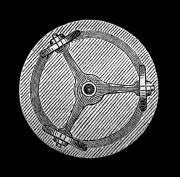
\includegraphics[width=0.5\textwidth]{images/fig46.png}
\label{fig46}
\end{figure}

Sometimes the clock has to be placed a long way below
the dials, $30$ or $40$~feet or more, and then it is necessary to
provide both for the weight and
the want of stiffness of such a
long leading-off rod; and this
is best done by a pair of friction
plates and rollers at the
top. The lower plate is set
on the beams which carry the
nests of bevelled wheels or
\textit{motion work:} on that lie three
small flat cheese-shaped rollers
on a horizontal tripod, with a
hole in it for the long rod to
go through quite loosely; and the other plate is fixed to the
top of the rod, which is in fact hung by it, the rollers carrying
the weight, and with no sensible friction on their own
centres, for the three-legged pivots have no weight upon
them. This kind of suspension is also used for heavy
%-----File: 242.png------------------------------------------
%-----Folio: 227---------------------------------------------
weathercocks which work a wind-dial inside the house, and
the ease with which a very heavy weight can be turned in
that way is surprising.

\subsection[Weathercocks.]{Weathercocks.}\markboth{WEATHERCOCKS.}{WEATHERCOCKS.}\label{subsec:Weathercocks.}\index{Weathercocks}---As these are generally fixed by clockmakers
in such cases as those last mentioned, I may as well
mention that a weathercock which is intended to answer
steadily to the wind, ought not only to be long in the vane
and thin in the tail, but equipoised; and so far from the vane
being perforated for ornament, it should be double, with the
two flat sides or vanes spreading out at a small angle from
the axis. When the cock works a dial it must be fixed to a
rod working loosely in a tube, and the top of the tube covered
with an inverted funnel on the rod; as also the rods or wires
which work the clock-hammers should be funnelled, over a
short pipe soldered to the leads, wherever they are exposed
to rain: otherwise the wires lead down the wet into the
clock. And the weights and ropes should be enclosed in a
case to keep them from the rain and wind, if they are in an
exposed place. (See also p.~\pageref{weathercocks}.)

\subsection[Ventilation of clock-room.]{Ventilation of clock-room.}\markboth{VENTILATION OF CLOCK-ROOM.}{VENTILATION OF CLOCK-ROOM.}\label{subsec:Ventilation_of_clock-room.}\index{Clock-room, ventilation of}\index{Ventilation of clock-rooms}---The clock-room at the
Exchange was at first made with the object of keeping out
the dust and damp in every possible way: even the slits in
the floor for the ropes had sliders to them; the clock was
enclosed in a glass case, the plate-glass cover originally
placed over the escapement being found not enough to keep
it from the damp. When the clock was repaired, and some
of the brass-work replaced with iron in 1854 (for a reason
which I shall mention hereafter), I suggested the removal of
all this glass, and encouraging instead of preventing a draught
through the room. This was done; and although the wet
used to stand in drops upon the clock before in damp weather,
it has been perfectly dry ever since. The same thing has
been found in small clock-cases: they may easily be too air-tight.
I do not mean that there is any objection to enclosing
a clock in a case, and of course it is absolutely necessary
%-----File: 243.png------------------------------------------
%-----Folio: 228---------------------------------------------
where the clock-room cannot be kept locked against everybody
but the man who has the care of it; only there should
be a draught through the room, and the case itself not too
close to let air through it. If the room can be kept warm
enough to prevent the damp from condensing on the clock it
is better still.
\section{TRAIN REMONTOIRES.}\label{sec:TRAIN_REMONTOIRES.}\index{Remontoire!train}\index{Train remontoires}\markboth{TRAIN REMONTOIRES.}{TRAIN REMONTOIRES.}

I have postponed this branch of the subject till I had gone
through all the more ordinary work of turret clocks.  A train
remontoire differs in principle from a remontoire escapement
(of which I have already treated) only to this extent: the
small weight or spring which gives the impulse to the pendulum
is not wound up at every beat, but at some longer
intervals, seldom more than half a minute; or the remontoire
work, you may say, is put one step farther back, acting on
the scapewheel instead of on the pendulum. So that if a train
remontoire of constant force and friction is made to act on a
dead scapewheel, the only variation of force to which the
pendulum is subject will be that arising from the pallet
friction. In small clocks the variations of the pallet friction
are generally much greater than of the train friction, and
therefore a remontoire would be of little or no use; but in
large clocks with heavy wheels and large hands to drive, the
contrary is the case; and there accordingly, either a train remontoire
or a remontoire escapement is of great use, provided
they really do what they profess---which many of them do
not.

The simplest form of train remontoire acting by a weight
is that described in \index{Reid on train remontoires|(}\index{Train remontoires!Reid's}Reid's book, on the endless chain principle,
which I have already described for a going barrel at p.~\pageref{endless}.
The scapewheel is not driven by the clock train, but it has a
spiked pulley on it which carries one loop of the endless
chain, and the other is carried by a similar pulley on an arbor
%-----File: 244.png--------------------------------------------
%-----Folio: 229-----------------------------------------------
driven by the train and turning in the same time as the scapewheel.
This remontoire arbor has a few long spikes sticking
out from it, at different distances along the arbor, and they
are just long enough to reach the middle of the scapewheel
arbor, and can slip past it through a nick cut for the purpose,
whenever that nick comes into the right position, which it
does once in every turn of the scapewheel; then the remontoire
arbor turns and winds up the endless chain a little
until the next spike falls against and is stopped by the scapewheel
arbor, till its nick also presents itself and lets that
spike slip through, as you see in this drawing.

Nevertheless, that construction is far from satisfying all
the conditions of a remontoire. The action of a chain
cannot be made smooth and uniform, and a rope or string
passing only half round a pulley is sure to slip in time, and
so the remontoire would fail. Moreover, Reid says that
although the Edinburgh clock went very well for a time, yet
it became necessary to remove the remontoire in consequence
of the banging of the spikes against the scapewheel arbor.\index{Reid on train remontoires|)}
That however would be easily cured by a fly; which may
now be considered a necessary element of every remontoire:
for there are several other kinds.

One is the bevelled wheel\index{Remontoire!bevelled wheel}\index{Train remontoires!bevelled wheel}\markboth{BEVELLED WHEEL REMONTOIRE.}{BEVELLED WHEEL REMONTOIRE.} remontoire, which was used in
many of the French turret clocks in the 1851 Exhibition. I
have already explained the principle of it, so far as the
bevelled wheels are concerned, at p.~\pageref{bev}; but something
more is now required. In fig.~\ref{fig47} (\textit{t.~o.}), consider the dark
disc $\mathrm{FG}$ and the pulleys omitted for the present (we shall
want them presently for something else). $\mathrm{X}$ is part of that
wheel of the clock which would naturally drive the scapewheel
$s$ if there were no remontoire, and if it were fixed to the arbor
of the pinion $t$ which $\mathrm{X}$ does drive. It also drives another
pinion $\mathrm{P}$ on an arbor $\mathrm{PQ}$ which I call the remontoire arbor,
because it carries two long spikes not quite in the same
straight line, or not at right angles to $\mathrm{PQ}$, which can pass
%-----File: 245.png--------------------------------------------
%-----Folio: 230-----------------------------------------------
\begin{figure}[htbp]
\centering\index{Fly, remontoire}
\caption{\sc Bevelled-wheel Remontoire}
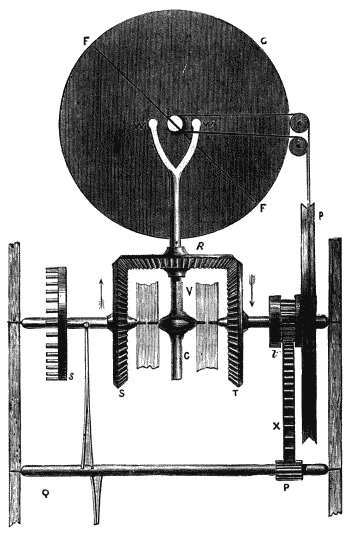
\includegraphics[height=535pt]{images/fig47.png}
\label{fig47}
\end{figure}
%-----File: 246.png--------------------------------------------
%-----Folio: 231-----------------------------------------------
alternately through two nicks in the scapewheel arbor. When
the arbor is stopped the train and the wheel $\mathrm{T}$ do not move;
but the weight of the middle bevelled wheel $\mathrm{R}$, with any weight
($+$ or $-$) attached to it, always presses down the far side of
wheel $\mathrm{S}$, and of the scapewheel s fixed on the same arbor,
and that force is practically constant. When the scapewheel
arbor lets a remontoire spike pass, the pinion $\mathrm{P}$ turns half
round and lets the train move a little, and lift up the right
side of wheel $\mathrm{R}$, and therefore lift up its centre half as
much, and then the other spike is held by the scapewheel
arbor. The fly may be driven by the wheel $\mathrm{D}$ anywhere,
either on the remontoire arbor or any other. We shall see
another way of driving it presently.

\subsection[Continuous motion remontoire.]{Continuous motion remontoire.}\markboth{CONTINUOUS MOTION REMONTOIRES.}{CONTINUOUS MOTION REMONTOIRES.}\label{subsec:Continuous_motion_remontoire.}\index{Remontoire!continuous motion}\index{Continuous motion clocks}\index{Train remontoires!continuous motion}\index{Wagner's continuous motion remontoire}---In connection with
this I will describe a remontoire exhibited in 1851, by
Messrs.~Wagner, the great turret clock makers of Paris, for
the purpose of getting a continuous motion for telescope-driving
clocks, or clocks to drive a barrel on which times of
observation may be recorded at less intervals than a second,
with all the advantage of a vibrating instead of a revolving
pendulum. The action for the vibrating pendulum which is
driven by the scapewheel $s$ is exactly what I just now
described, except that there is no spike wheel and no sudden
letting off. Instead of that there is a large pulley $p$ on the
arbor of the wheel $\mathrm{T}$ which lifts the remontoire arm $\mathrm{VRW}$\@.
This pulley drives a much smaller one on the arbor of a fly
$\mathrm{FF}$, which runs inside a tin drum without a bottom, which
is hung over it by two wires $\mathrm{WW}$ from the end of the remontoire
arm. The weight of the drum is counterpoised so
as not to let it preponderate too much. The fly is the thing
which regulates the velocity of the clock train, which is
always moving; the farther the drum falls over it and cuts
off the air within from the air outside, the faster the fly will
turn, and vice vers\^{a}; and things are so adjusted that the
continuous motion of the clock train driving the fly will just
%-----File: 247.png-----------------------------------------------
%-----Folio: 232--------------------------------------------------
keep pace with the average motion of the scapewheel driving
the pendulum by beats as usual. If the clock falls behind
the proper speed the remontoire wheel and its drum falls a
little and lets the fly go quicker, and if too fast it rises and
the velocity of the fly is checked. The one in the Exhibition
seemed to go very steadily; and as there is nothing in all
this at all difficult to make, I am surprised that more complicated
contrivances should be used for such purposes as I
have mentioned.

Mr.~De~la~Rue\index{De~la~Rue's telescope-driving clocks}\index{Telescope-driving clocks!Cooke's, Bond's, and De la Rue's}\markboth{FOR DRIVING TELESCOPES.}{FOR DRIVING TELESCOPES.} and Mr.~Cooke\index{Cooke!his telescope-driving clock}\label{telescope} appear to have hit simultaneously
on the following plan for a telescope-driving
clock, which retains the advantage of a vibrating pendulum,
and may have a gravity escapement also. In the figure at
p.~\pageref{fig47} suppose the two opposite bevelled wheels to be respectively
fixed on the `centre arbors' of two clock trains,
the left hand one ending in a vibrating pendulum, and the
right in a conical pendulum or a fly. And let the arbor of
the intermediate wheel (omitting all the wind apparatus
$FGF$) be held by a spring instead of the constant weight
$\mathrm{C}$\@. At every beat of the pendulum the left hand train will
stop for a moment, but the fly-wheel train, of which the
barrel is to drive the telescope, will go on by its own
momentum, and because the spring allows the intermediate
wheel, and therefore the right hand wheel and its train, to
move a little. If that train is inclined to go too fast, the
spring will diminish the force upon it; and if too slow, will
increase it. Of course the weight and fly are to be adjusted
so as to make that train go naturally as nearly as possible
with the other.

A still simpler telescope-driver was invented by Mr.~R.~F.~Bond\index{Bond's telescope-driving clock},
of Boston, U.S., brother of the well-known Professor
of Astronomy there. As I understand the description, one
arbor of the clock has two wheels on it, one fixed, and the
other connected with it by a spiral spring. The second of
these wheels is either the scapewheel or the one below it,
%-----File: 248.png-----------------------------------------------
%-----Folio: 233--------------------------------------------------
and the other ultimately drives a fly, which allows the train
to so continuously, the spring equalising the force sufficiently
every beat. Mr.~Cooke said it did not answer, but
Mr.~Bond replied with a testimonial from the late Rev.~W.~R.~Dawes,
F.R.A.S., who had the reputation of being
the best observer of his time, that the `performance was
exquisite; that it kept the thread of the micrometer
dividing a star for nearly an hour together with a magnifying
power of $800$ or $1000$ on, and that no jerk or
interruption was perceptible.' Lord Lindsay, P.R.A.S.,
invented another, too complicated to describe here, on the
ground that neither Cooke's nor Bond's clocks would drive a
large telescope fitted with spectroscopic apparatus steadily
enough for that purpose.\footnote{All these contrivances are described in the R.A.S. Notices,
vols.~27 and 33, and \textit{Horological Journal}, of February and
April 1868.}

The Royal Exchange\index{Dent, E.~J.!Royal Exchange clock}\index{Exchange, Royal!clock} clock was originally made with a
gravity remontoire, though it was afterwards altered.
Instead of bevelled wheels, Mr.~Dent used an \textit{internal} \index{Remontoire!internal wheel}\index{Train remontoires!internal wheel}\markboth{INTERNAL WHEEL REMONTOIRE.}{INTERNAL WHEEL REMONTOIRE.}wheel,
\textit{i.e.}\ one with teeth on the inside of the rim, instead of the
outside. That wheel $\mathrm{D}$ (fig.~\ref{fig48}, \textit{t.~o.}) had the letting off spikes
on its outside; at least a wheel on the same arbor had,
which is the same thing. It was driven by the centre
wheel of the clock, and whenever it moved it lifted the
remontoire arm and weight by means of the small wheel $\mathrm{B}$
lying between the internal teeth and the wheel $\mathrm{C}$ on the
arbor of the wheel $\mathrm{F}$ which drove the scapewheel: that
arbor being of course independent of, though in the same
line with the arbor of the wheel $\mathrm{D}$ and its pinion. The
remontoire was let off at every $20$~seconds; which however
is not so good an interval as $30$, because it is not easy to
distinguish whether the hands are pointing to $10$~seconds
before or $10$~seconds after the half minute; whereas it is
perfectly easy to see whether they are pointing to a minute
%-----File: 249.png-----------------------------------------------
%-----Folio: 234--------------------------------------------------
or a half-minute, if the dial is properly made, as  I have
already described. This facility for taking the exact time
from the dial by the jump of the hands is one of the advantages
of a train remontoire, where the momentum of the
hands is not too great.

\begin{figure}[htbp]
\centering
\caption{\sc Royal Exchange Remontoire}
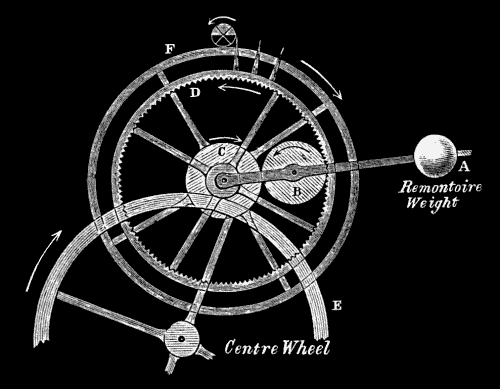
\includegraphics[width=\textwidth]{images/fig48.png}
\label{fig48}
\end{figure}

There \markboth{SIMPLEST TRAIN REMONTOIRE.}{SIMPLEST TRAIN REMONTOIRE.}is yet another way of making a train remontoire
without either bevelled or internal wheels. In fig.~\ref{fig49} (next
page) $\mathrm{E}$ is the scapewheel, and $e$ its pinion driven by the
remontoire wheel $\mathrm{D}$ which rides with its pinion $d$ fixed to it
on a stud in the remontoire lever AP\@. The centre wheel $\mathrm{C}$
drives that pinion and a smaller one $g$ on a wheel which
drives another pinion $f$ on the fly arbor, which has also the
remontoire spikes $\mathrm{AB}$ attached to it. The numbers of the
teeth are so arranged that the fly will turn once for each
turn of the scapewheel, and the scapewheel arbor has only
%-----File: 250.png-----------------------------------------------
%-----Folio: 235--------------------------------------------------
two notches in it, so as to let off one remontoire spike every
seconds. It is evident that the scapewheel is always
\begin{sidewaysfigure}[p]
\centering
\caption{\sc Simplest Train Remontoire}\label{fig49}
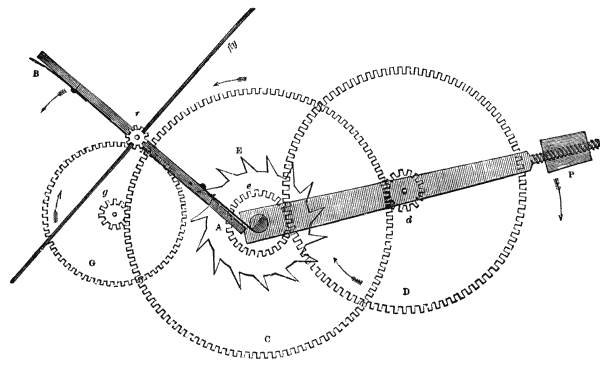
\includegraphics[width=\textwidth]{images/fig49.png}
\end{sidewaysfigure}
%-----File: 251.png--------------------------------------------
%-----Folio: 236-----------------------------------------------
driven by the remontoire wheels and weight, and not affected
by the clock train. There were several French clocks of
this construction in the Exhibition of 1851, but they all
had the fly driven by an endless screw, which is objectionable
because it involves an immense amount of friction
and the motion of the train was so slow that you could
hardly distinguish the jump of the hands.

\subsection[Spring Remontoire.]{Spring Remontoire.}\markboth{SPRING REMONTOIRE.}{SPRING REMONTOIRE.}\label{subsec:Spring_Remontoire.}\index{Remontoire!spring}\index{Spring!remontoires}\index{Train remontoires!spring}---But it must be observed that all
these gravity remontoires are still subject to the friction of
the remontoire wheels themselves, which is not inconsiderable,
although it is much less, and less variable, than
that of the clock train and hands. To avoid this, it was
long ago attempted to contrive a spiral spring remontoire
which would drive the scapewheel without any sensible
friction. One of these is described in Reid's article in the
seventh edition of the \textit{Encyclop\ae dia Britannica}; and another
was invented by Sir G.~Airy\index{Airy, Sir G.~B.!spring remontoire},\footnote{See \textit{Horological Journal}, xvii.~22.} and two or three specimens
of it were made by old Mr.~Dent. They all went on the
plan of connecting two wheels, or a wheel and pinion, on the
same arbor by a spiral spring, one being fixed to the arbor
and the other riding upon it; and the consequence was that
the scapewheel was always subject to the friction of the
other wheel set upon its arbor and pressed tight upon it by
the action of the spring, which was probably worse than the
ordinary friction of the train; and they were all failures.

This difficulty however may be got over by a very simple
contrivance which I\index{Beckett, Sir E.!spring remontoire} invented in 1849, and which was used
in several large clocks, and would have been in many more
but for its having been superseded by the cheaper and
simpler gravity escapement already described (p.~\pageref{subsec:Sir_E.Beckett's_Gravity_Escapements.} to
\pageref{gravend}). In fig.~\ref{fig50} (next page) $\mathrm{E}$ is the scapewheel and $e$ its
pinion, not fixed to the arbor of $\mathrm{E}$ nor riding upon it, but
upon an independent stud $k$ screwed to the clock frame. In
front of the pinion a small bush is pinned on to the same
%-----File: 252.png--------------------------------------------
%-----Folio: 237-----------------------------------------------
stud which carries the pivot of the scapewheel arbor, on
which is set a large watch spring $s$, of which the outer end
is held by a pin $h$ screwed into a small plate fixed to the
\begin{figure}[hbtp]
\centering\index{Fly, remontoire}
\caption{\sc Sir E.~Beckett's Spring Remontoire}
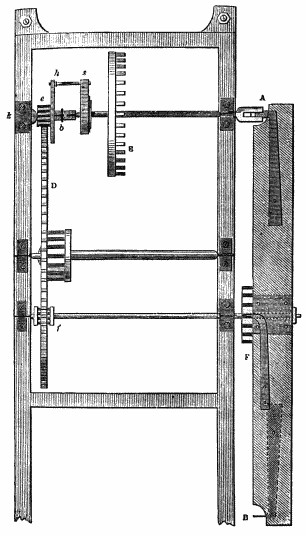
\includegraphics[height=535pt]{images/fig50.png}\index{Remontoire!spring}\index{Spring!remontoires}\index{Train remontoires!spring}
\label{fig50}
\end{figure}
%-----File: 253.png--------------------------------------------
%-----Folio: 238-----------------------------------------------
front of the pinion, so that the pinion acts on the scapewheel
by the intervention of this spring without any friction
except that of the coils of the spring upon each other,
if they touch at all. The wheel $\mathrm{D}$ which drives that pinion
also drives another on the fly arbor $f$. If the scapewheel
turns in a minute, there will be two nicks across its arbor,
as in fig.~\ref{fig47}, for the remontoire spikes or stopping springs
to act upon. But if it turns in two minutes, as the pin
scapewheels generally do, a different plan is adopted: the
scapewheel arbor is then brought through to the front of
the clock frame and has a small steel cylinder set upon
it, with two nicks across its face, not its side, one broad
and shallow and the other deep and narrow; the remontoire
springs set on the two arms of the fly have corresponding
shapes, so that one will pass through the broad
nick only and be stopped by the narrow one, and the other
will pass through the deep nick but be stopped by the
shallow one. The fly in this case makes half a turn for
every quarter turn of the scapewheel, and therefore its
pinion must be only half the size of the scapewheel pinion.
In very large clocks such as the Exchange, in which the
gravity remontoire was replaced\markboth{ALTERATION OF EXCHANGE CLOCK.}{ALTERATION OF EXCHANGE CLOCK.} by a spring one in 1854,
the fly is made separate from the remontoire arms, with
a ratchet and click as usual to let it run on a little by
its own momentum; but in smaller ones it does very well
to put the remontoire spring stops on the fly itself.

The wheel shown at $\mathrm{F}$ with a kind of detent in it, is for
setting up or letting down the spring with reference to the
remontoire arms, and so increasing or diminishing the force
on the scapewheel.

This was the construction of old Mr.~Dent's\index{Dent, E.~J.!Exhibition clock} large clock in
the 1851 Exhibition, now at King's Cross\index{King's Cross clock} station, which was
found only $3$~seconds \index{Rate!of 1851 Exhibition Clock}wrong at the closing of the Exhibition,
though it had never been altered during the $24$~weeks it was
there, after its preliminary regulation. I never knew any clock
%-----File: 254.png--------------------------------------------
%-----Folio: 239-----------------------------------------------
with such a rate as that, and yet it has only a common
unjewelled pin-wheel escapement, and a $1\frac12$~sec.\ zinc and
iron pendulum, and most of the wheels are of cast iron. It
has sometimes gone since for several months together
without any noticeable variation.

The Exchange\index{Exchange, Royal!clock!alterations of} clock was immensely improved by that
alteration, and made as good as that of the King's Cross
clock in general, but I have no exact record of its rate.
I must confess however, that this kind of remontoire is
not safe to put into clocks left in any common hands, as I
have found by experience that the first time the clock wants
cleaning or repairing---or even without that opportunity---a
stupid workman, or master, makes a point of destroying the
remontoire. I knew one case where it was done as soon as
an ordinary clockmaker got the care of it---and that at
Manchester, the city of machinery. This cannot happen
with a gravity escapement, which is also much cheaper.
The Exchange clock has been altered by Gillett and Bland
to the double three-legged gravity escapement, which is now
the standard one for all large\index{Gravity escapements!best for large clocks} clocks. Therefore it is no
longer necessary to explain further details of the spring
remontoire, as in former editions.

\subsection[Cast-iron wheels.]{Cast-iron wheels.}\markboth{CAST-IRON WHEELS.}{CAST-IRON WHEELS.}\label{subsec:Cast-iron_wheels.}\index{Cast iron!for clock wheels}\index{Wheels for clocks!cast iron}---The success of the contrivances for
cutting off the variations of force from the pendulum led to
another alteration which helped to reduce the price of large
clocks considerably; and that was the making all the wheels
below the escapement, and all the dial wheels, of cast iron
instead of brass or gunmetal. Mr.~Vulliamy had before
recommended that as a good construction for cheap clocks,
but it had always been thought that they could not be also
good ones on account of the greater friction of the train.
I believe that apprehension was very much exaggerated, even
for clocks of the common construction, provided of course
the escapement is light and well made; but as soon as you
cut off the friction of the train from affecting the escapement
it is obvious that cast-iron wheels are just as good as brass
%-----File: 255.png--------------------------------------------
%-----Folio: 240-----------------------------------------------
or gun-metal. The clockmakers in general violently denounced
it, probably for no better reason than that it
lowered their prices enormously, the price being now only
\pounds 200 for clocks of greater power and far greater accuracy
than those for which \pounds 500 used to be charged not many
years ago.

The cast iron wheel controversy came to a head in some
of the Lancashire papers soon after the making of the clock,
from my design, for the Manchester Infirmary; and the
advocates of brass wheels had clearly no case whatever.
Their three points against cast iron were friction, rust, and
liability to break. The friction of the train is absolutely
immaterial with a remontoire, or a gravity escapement, and
no large clock can go with great accuracy without some
such contrivance. The next objection is obvious nonsense,
because all except the acting surfaces are painted, and they
are of course oiled as in all other iron wheel machinery.
The liability to break is a mere question of experience.
Those who condemn them for clocks must be very ignorant
of the extent to which cast iron wheels finer than are ever
used in church clocks are used in every factory in Yorkshire
and Lancashire. I made particular inquiries once as to the
sizes down to which the teeth are cast in iron wheels for
spinning machinery (for that is what I mean by cast iron
wheels), and I found that they are cast with quite sufficient
accuracy with teeth as small as $\frac{1}{10}$~inch thick;  which is
smaller than any I have seen used in clocks, because there
is very little saving in cost in using iron wheels so small as
that. The great saving of course is in the large wheels of
the train, and the dial and bevelled wheels, of which a good
many of the same pattern and no very fine pitch are required.

Before I leave the cast iron wheels I should observe that
they work better with cast iron pinions\index{Cast iron!for steel pinions} than with steel
ones: indeed cast iron and steel seem never to work well
together, at least in no clock-work that I am acquainted
%-----File: 256.png--------------------------------------------
%-----Folio: 241-----------------------------------------------
with if there is much pressure between them. I have seen
cast iron fly ratchets used with steel clicks, by clockmakers
who would not listen to the proposal of iron wheels and
pinions for any but the commonest clocks, and they had to
be removed, and replaced either by wrought iron or brass
ones. I have seen and heard of brass teeth worn out in
an almost incredibly short time, long before iron teeth in
the same clock showed any signs of wearing. Moreover
few people have any idea how rapidly brass is corroded
and in fact destroyed\label{decay} by such an atmosphere\index{Brass-work destroyed by town atmosphere} as that of
London and other large towns. I have several times seen
the brass tubes which had been used in dial work, and thin
pieces of brass elsewhere, brought back to be replaced with
iron because they had become completely rotten. It was
so at the Royal Exchange in eight years.

In this respect gun-metal\index{Gun metal!its composition}\markboth{CAST IRON AND GUN-METAL.}{CAST IRON AND GUN-METAL.} is better, which is copper and
tin instead of copper and zinc, but for large wheels\index{Gun metal!for clock wheels} it is no
way superior to iron; and it is generally made too soft.
It is equally absurd to polish iron work, except the acting
surfaces; that rusts even sooner than brass begins to corrode;
in fact very often in a week after the clock is put up.
Then somebody who has the care of it floods it all with oil,
and it is filthy ever after. The only proper rule to lay down
is that \textit{all non-acting surfaces should be painted}\index{Painting!all ironwork of large clocks}. In the
Westminster clock even the small brass wheels in the
escapement are painted like the iron ones.

The truth is that all this `finishing'\index{Finishing@`Finishing' too much undesirable}\markboth{`FINISHING' AND JOBBING.}{`FINISHING' AND JOBBING.} of non-acting surfaces
is what old Dent used to call `working for fools.' It has
literally no other object (as plenty of clockmakers have
confessed to me) than to make an impression on the `fools'
(in and out of the trade) who go to see a new clock in the
first month after it is put up, and never see or want to see
it again. Such people as these think it a much finer thing to
have a clock look bright for a month and never keep time
within a minute a week---or a day, for what they know---than
%-----File: 257.png--------------------------------------------
%-----Folio: 242-----------------------------------------------
`to look like a patent mangle,' but keep time within a
second a week.

I must warn people however against some altogether
cast-iron clocks which got into vogue some years ago by
their extreme cheapness, if they could be called cheap at
any price. I heard constant complaints of them, and had
to subscribe once to help a friend to get rid of one and
substitute another of a proper kind. I shall give presently a
form of specification showing how much of a large clock
may be of cast-iron.

A few years ago I learnt when it was too late that a
deputation from the corporation of a considerable town had
come to London to negotiate for a first-rate town-hall clock,
and after wandering about for some time they fell into the
hands of `an eminent firm' who boast of sending clocks all
over the world, and engaged to pay them more than would
have bought the best possible clock for one which was
warranted to keep time within $5$~\textit{minutes} (not seconds)
a week; whether it actually does perform that feat I do not
know, but I heard casually of some other of its successes,
which gave hopes of it breaking down altogether.

Another common cause of bad church clock making is the
inveterate habit of \index{Jobbing in contracts for public clocks}\label{jobbing}jobbing for the benefit of a townsman by
giving the order to a watchmaker who never made a turret
clock in his life, and who immediately goes or writes to one
of the few real makers for the cheapest clock that will serve
his purpose, and probably charges for it as much as the
people could have got a first-rate one for, if they had had a
competition of the best real makers of large clocks, or even
gone to one of them alone. The local watchmaker, by way
of carrying out the fraud completely, generally insists on the
real maker putting, not his own, but the pretender's name
on the clock. If this were merely a question between the
makers who consent to do so, and those who will not, I
should leave them to find their own remedy; but as it
%-----File: 258.png--------------------------------------------
%-----Folio: 243-----------------------------------------------
affects the general credit of our public clocks, I think it
right to give this warning, though it will probably not be
read by one in a hundred, or attended to by one in a
thousand, of those for whom it is intended. It would be far
better to do the `native talent' job in a straight-forward
way by letting the local watchmakers draw lots for a \textit{bonus}
of \pounds 20, and then advertise for tenders under proper conditions,
such as I suggest below.

The practice of insisting on clockmakers tendering for
bells, except quite small and common ones, is almost equally
objectionable. Every now and then, one party or the other
has paid dearly for it themselves; for which also I do not
care; but the more material thing is, first that two profits
have to be got out of the transaction without any real
necessity for a middle man, and that there is practically much
less responsibility and control than when you deal directly
with the bell-founder. You might as well insist on the clockmaker
fitting up an observatory with telescopes,\footnote{There was indeed
one clockmaker quite competent to do both, the
late Mr.~Cooke\index{Cooke!clock and telescope maker}, of York; but then he made the telescopes himself,
and was one of the best makers of his time.} or trust a
builder to put in painted windows and the organ in a church.




\section{SPECIFICATIONS FOR PUBLIC CLOCKS.}\label{sec:SPECIFICATIONS_FOR_PUBLIC_CLOCKS.}\index{Specifications!for public clocks}\index{Turret clocks!specification for}\markboth{SPECIFICATIONS FOR PUBLIC CLOCKS.}{SPECIFICATIONS FOR PUBLIC CLOCKS.}


Every now and then I happen to see specifications for
large clocks, either prepared by somebody belonging to the
office which has to order it, or in the form of a tender sent
in by some advertising clockmaker, and I hardly know which
are generally the worst, except that the author of the tender
does know what he is about, and takes care to put in as
many adjectives and as few substantives as he can, and the
author of the specification never does know what he is about.
An elaborate specimen of this kind was shown to me some
years ago, from a Government office, which stipulated among
%-----File: 259.png--------------------------------------------
%-----Folio: 244-----------------------------------------------
other remarkable things, that the pendulum was `to vibrate
$2$~seconds, but to be as long as the room admitted of.' It
was also to have \textit{convex} copper dials a \textit{quarter} of an inch
thick, and a \textit{dead} escapement; which were three specimens
of the author's practical knowledge of the present state
of science. The specification, though of many pages, did
not contain a single thing, except the probably impossible
pendulum, of the slightest value towards securing
what (I suppose) was wanted, either in the way of time-keeping
or striking. Sometimes the providing of a clock and
bells is entrusted to the architect, by people who are not
aware that modern architects rather boast than are ashamed
of being totally ignorant of every thing of the kind. I have
heard people who ought to know better say, that `the only
way is to throw all the responsibility of everything connected
with the building on the architect,' and utterly puzzled when
I asked them what those fine words meant, or what would
they do if everything turned out wrong, as it generally does
in that case. I will therefore give a specimen of the
specification suitable for a large church clock, though I cannot
adapt it to all possible circumstances; and a much stricter
one is requisite for a general competition than for one
limited to a few makers whose work I know to be of the best
kind. Indeed no specification can secure a good clock from
a bad clockmaker\index{Jobbing in contracts for public clocks}; and it ought not to be necessary to warn
people (but I find it is) that those who blow their own trumpet
loudest in advertisements are very often the least to be trusted,
especially in an article of which most purchasers are quite
incapable of judging, until it is too late. All that a stringent
specification can do is to frighten away bad makers from
tendering at all; and for that purpose the first clause of the
following form is useful in a general competition, provided
is certain to be enforced.
\begin{enumerate}
\item To  make and fix  a clock with $m$ dials of $n$ feet
diameter, and striking the hours and Westminster quarters,
%-----File: 260.png--------------------------------------------
%-----Folio: 245-----------------------------------------------
on bells which are or would be the 2nd, 3rd, 4th, 7th, and
tenor of a peal of $8$, the tenor weighing ------.

\item The dials to be concave and made of copper, or painted
on the wall, if smooth enough, or with the figures and
minutes of cast iron, in rings. If the dials are to be illuminated
they \textit{must} be of cast iron, and should have opal glass
$22$~oz.\ to the foot, except behind the minutes, which may
be $16$~oz.\ to the foot. There must be no straight radiating
pieces of iron in the middle. [Architects should be made to
understand (if possible) that dials intended to be illuminated
must have a clear opening in the wall of the full diameter of
the dial.]

\item The long hands to have a short external counterpoise,
painted the same colour as the dial, if not illuminated, and
the hands, figures, and minutes to be gilt. If illuminated,
the hands, figures, and minutes to be black, and all the rest
gilt. The long hands to be straight and plain.

\item The escapement to be the double three-legged gravity,
and care must be taken to leave room for the fly of sufficient
length, and to make the angles such as to run no risk of
tripping, and generally according to this book.

\item  The pendulum to have zinc compensation with iron
rod and tube, and bob not less than $2$~cwt. To beat $1\frac12$
seconds for a clock with several large dials, but may be $1\frac14$
for a smaller clock, or if there is no room for a $1\frac12$~second
pendulum. It is to swing $2\frac12^\circ$ from zero, and to have a
block under it in case the spring breaks, and a degree plate.

\item The clock must lie on stone corbels or iron beams, or
brackets bolted through the wall, and the pendulum cock
either bolted to the wall, or rising from the clock-frame,
which is to be generally on the plan at p.~\pageref{fig40} of this book;
but the great wheel arbors are to be in drop bushes of the
form $d$, at p.~\pageref{fig38}.

\item There is to be a minute dial, and either one for seconds
or a wheel marked for that purpose, with a fixed index.
%-----File: 261.png--------------------------------------------
%-----Folio: 246-----------------------------------------------

\item To have the improved bolt and shutter maintaining
power (p.~\pageref{smallmaintain}) or the Westminster one for a very large clock
The going part to go a little over eight days.

\item The striking parts\index{Striking part!of turret clocks} to be wound up every one or two days,
except in small clocks [or they will never strike efficiently].
All the striking to be done by steel-faced cams on the great
wheels. The 4th quarter bell to have two hammers (see
p.~\pageref{2hammer}). In smaller clocks cast-iron cams will do.

\item The hour striking to be let off independently of the
quarters, and the first blow to be struck exactly at the hour,
the hammer being left on the lift: the other quarters to
begin exactly at $15$, $30$, and $45$~minutes.

\item \index{Hammers, clock!weight}The hour hammer to be not less than a $60$th of the
weight of the bell, and to be raised not less than $9$~inches;
the quarter hammers to increase in weight upwards from a
$60$th to a $40$th of the weight of their bells, and all the
hammers to be raised enough to bring the full tone out of
the bells: small ones at least $6$~in., and the hour one at least $9$.

\item There must be either levers or eccentrics to lift the
hammer levers completely off the cams, when the bells are
ringing, if there is a peal.

\item The small wheels of the going part to be of brass or
hard gun-metal, driving lantern pinions. All the larger wheels
and the pinions driven by them may be of cast iron, and their
being of brass or gun-metal will be considered no reason for
a higher price. All bushes to be brass or gun-metal. The
large pivots to be case-hardened, the smaller ones and their
arbors to be of steel. The pulleys to be large and pivotted
in brass bushes.

\item The barrels of sheet iron brazed, with iron or steel
wire ropes \textit{not} coated with zinc [which makes them crack],
and the pulleys to be so placed that the ropes do not grind,
or go twice over the barrel.

\item The flies not to be in front of the clock, and to be long
enough to make the time of striking quite uniform, and slow
%-----File: 262.png--------------------------------------------
%-----Folio: 247-----------------------------------------------
enough. The fly ratchets to be either squared or keyed on,
and not merely pinned. The ratchets \textit{not} to be of cast iron,
and each to have two clicks. [Many smashes have occurred
for want of attention to these two conditions.]

\item All the iron-work except acting surfaces to be painted
blue [black is more difficult to see if anything is wrong, and
if not painted iron only gets rusty].

\item If the weights go out of sight there must be something
to stop or warn against winding them too far. And
also a large box with $3$~feet deep of small stones, to catch
the weights if they fall; unless they go down to the ground
of the tower, when they can only break flags.

\item All wheels to take out separately by unscrewing the
bushes; and pulleys to be placed where they can be oiled.

\item On all points not specified, the clock is to be made
according to the directions of this book, applicable to clocks
of the kind now required.

\item The clockmaker to provide (or design and superintend)
a strong wooden case for the clock, with glass showing the
minute dial if it is in the belfry, and so arranged that the
striking parts can be wound without opening the case;
unless the clock is in a room always locked up, and protected
from weather. In many places it is necessary to
have a case for the weights, and pulleys at the top, if
exposed in a bell-chamber.

\item The estimate to state the cost of the clock and dials,
and of the fixing, case, \&c., separately.

\item \label{degerr}Half the price to be paid on the clock being completed,
to the satisfaction of such person, not objected to for
good reasons assigned by the clockmaker, as the committee
may appoint, and \textit{the other half when it has gone for three
calendar months continuously, without varying more than five
seconds in any week}---tested by the striking of the first blow
of any hour. [This is an ample margin to allow now that we
know from the Westminster and other clocks that they may
%-----File: 263.png--------------------------------------------
%-----Folio: 248-----------------------------------------------
be made to go without much more than a second a week
variation. Every town now has the means of testing its
clocks by electric telegraph time at the post office, but not
so exactly as it ought to be. And if there is any neighbouring
observatory, or meridian instrument, properly attended
to, that is much better.]
\end{enumerate}




\section{CONSTRUCTION OF THE WESTMINSTER CLOCK.}\label{sec:CONSTRUCTION_OF_THE_WESTMINSTER_CLOCK.}\index{Westminster clock!construction}\markboth{THE WESTMINSTER CLOCK.}{THE WESTMINSTER CLOCK.}


The frontispiece of this book is a front elevation of this
great clock, or so much of it as can be shown in one view
without confusion, for which purpose I have drawn the
wheels and pinions only as circles. As I have inserted the
numbers of the teeth, and the size of all the parts may be
taken from the scale, I shall say no more than that the
frame is $15\frac12$~feet long and $4$~feet $7$~inches wide. The
going part does not occupy above $2$~feet of this width, the
front bushes of the wheels being carried on a separate bar
lying on the two cross pieces of which the ends are shown
in the drawing bolted to the great back and front girders.

\subsection[Double-barrelled Crab.]{Double-barrelled Crab.}\markboth{DOUBLE-BARRELLED CRAB.}{DOUBLE-BARRELLED CRAB.}\label{subsec:Double-barrelled_Crab.}\index{Crab, double-barrelled}\index{Double-barrelled crab}---The space between the front
of the going part and of the great frame happens to be convenient
for the fall of the ropes from a double-barrelled
crab (fig.~\ref{fig51} next page), which is fixed upon the iron beams
$\mathrm{BB}$ which go across the room from east to west to carry
the `motion work' or nests of bevelled wheels above the
clock, of which the first pair are shown in the drawing.
This crab is the only means of getting anything into the
clock room which is too heavy to be carried by a man
up the stairs. It consists of two small equal barrels, with
four pulley grooves in each, each having an equal wheel
at the end turned by equal pinions on the winding arbor.
The rope passes over the outer halves of the two barrels
$4$ times, one end falling down the clock shaft or well for
the weights while the other rises; and it can either be used
%-----File: 264.png--------------------------------------------
%-----Folio: 249-----------------------------------------------
\begin{figure}[htbp]
\centering
\caption{\sc Double-barrelled Crab}
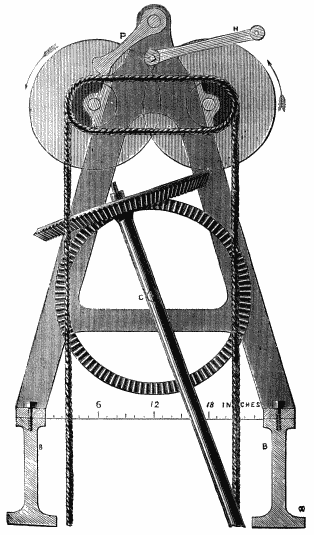
\includegraphics[height=535pt]{images/fig51.png}
\label{fig51}
\end{figure}
%-----File: 265.png--------------------------------------------
%-----Folio: 250-----------------------------------------------
with a single rope, or with pulleys. The \textit{pall} $\mathrm{P}$ is in effect a
silent click to hold the rope when the handle $\mathrm{H}$ is let go;
and it will turn over on the horizontal pillar at the top of the
crab, to act the opposite way when the barrels are worked
the other way.

The great advantage of it is that it avoids the crowding
and overlaying of a long rope on the barrel, which makes the
work harder at every fresh `overlay,' as it practically increases
the diameter of the barrel; and that becomes so intolerable that
the plan of pulling off the rope by hand after three or four coils
on the barrel has to be resorted to in long lifts; and that
again involves the difficulty of having to slide the coils back
to the beginning of the barrel, holding the rope by the hands
of several men, or by some supplementary machinery, for
very great weights, as was done with Big Ben in 1859. `Great
Paul' was raised on 3~May, 1882, by a double-barrelled crab,
or rather two of them, and pulley blocks besides; with only
this difference, that the ropes were crossed between the
barrels to give greater frictional hold; but that also causes
a considerable friction of the ropes against each other, and is
really unnecessary. A crab like this, not with the ropes
crossed, driven by steam, was used for taking up the ribs of
the great domes of the 1862 Exhibition. I had recommended
it in the 1860 edition for taking up heavy bells,\footnote{The differential pulley with an endless chain in notched grooves is
now largely used for moderately heavy weights, the chain being pulled
by hand as in the old-fashioned $30$-hour clocks; but it will not do for
great weights.} and in the
later editions I suggested a further improvement, shown in
fig.~\ref{fig52} (next page), by putting the pinions right in the middle
between the wheels, and making them all roll on blank `pitch
circles' (see chapter on teeth of wheels), besides having small
teeth cast by the side of the circles. This will take a great
deal of pressure off the barrel pivots, and also off the driving
pivots where it does mischief, and transfer it to the rolling
circles, where it is useful in driving and relieves the teeth,
%-----File: 266.png--------------------------------------------
%-----Folio: 251-----------------------------------------------
and would almost drive without any. They may consequently
be made much smaller, and the wheels also, and yet
with the same power as a much larger crab of the common
kind; especially if $4$ wheels are used: which also has the
advantage of relieving all the pivots equally. $18$~inch wheels
with $1\frac12$~inch pinions would be strong enough for all ordinary
work of single multiplying crabs. And it is easy to add
another wheel and pinion for larger ones.
\begin{figure}[htbp]
\centering
\caption{\sc Another form of Double-barrelled Crab}
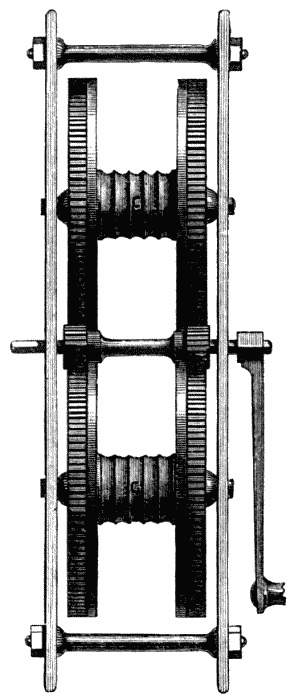
\includegraphics[height=0.7\textheight]{images/fig52.png}
\label{fig52}
\end{figure}
%-----File: 267.png--------------------------------------------
%-----Folio: 252-----------------------------------------------

The teeth of the pinions and wheels respectively should be
made as will be explained under `Teeth of Wheels,' the
pinion teeth alone projecting beyond the pitch circle. The
rolling circles must be hard, or they will bruise each other.
The arrangement of the frame also will depend on the work
for which the crab is intended; I only show what affects
its principle. The horrible noise of the common \textit{pall} may
be avoided by putting a wedge-shaped one between any two
of the rolling circles, with a slight spring acting on it,
according to the direction of driving for the time. This will
act as a silent pall as soon as you let go the handle.

Returning to the clock, the back of the frame is $2$~feet
$5$~inches from the west wall of the room, which is the east
wall of the ventilating chimney or air-shaft of the Houses of
Parliament running all the way up the tower. The room is
$28$~feet by $18$, and the clock lies, as shown in the drawing,
on the north and south walls of the shaft or well for the
weights, which is $174$~feet high, and the floor of the room is
$2\frac12$~feet below the top of two iron plates which cover the
walls and are spread out behind and built in quite through
the wall of the airshaft, so as to prevent any possibility of
endway motion of the clock frame, which is bolted to the
plates. The pendulum cock is a large frame
work cast in one piece and also built in through the wall,
quite independent of the clock frame. The pendulum
chamber is made of sheet iron within the weight shaft, in
order to protect the pendulum from the wind: you can
descend into it by a ladder and a trap-door; which can
seldom be wanted, as there is a degree plate set on the floor
under the clock, which is a little lower than the general floor
of the room, and is covered with a grating lying on the
beams which carry the returned end of the ropes.

\subsection[Regulation.]{Regulation.}\markboth{REGULATION OF THE CLOCK.}{REGULATION OF THE CLOCK.}\label{subsec:Regulation.}\index{Westminster clock!regulation of the pendulum}---The mode of regulating the pendulum
by small weights has been sufficiently described at p.~\pageref{accelerate}.
Whenever a larger alteration is required, in consequence of
%-----File: 268.png--------------------------------------------
%-----Folio: 253-----------------------------------------------
thunder-storms or an accidental disturbance of the pendulum,
either stopping the scapewheel or letting it trip one beat by
lifting a pallet alters it $4$~seconds, whereas you cannot put a
dead escapement forward at all, nor stop it without considerable
risk of spoiling a tooth.

The pendulum weighs altogether very nearly $700$~lbs., of
which the bob is about $4$~cwt. In other respects it has been
already described at p.~\pageref{subsec:Suspension_of_pendulums.}. The spring is a $60$th of an
inch thick and $3$~inches wide, and the free part of it $5$~inches
long. The great pin through the upper chops has nuts on
its ends to adjust it to the exact centre between the pallet
arbors. Those are not shown at page~\pageref{fig09}, because they are
not generally used. The pendulum\index{Pendulum2@Pendulum!of the Westminster clock} cock, and the position
of the floor behind the clock, are so arranged that a tall man
can stand with his head inside the cheeks of the cock so as
to look square at the escapement\index{Gravity escapements!in the Westminster clock}; which is

\subsection[The double three-legged gravity escapement,]{The double three-legged gravity escapement,}\markboth{THE DOUBLE THREE-LEGGED GRAVITY ESCAPEMENT.}{THE DOUBLE THREE-LEGGED GRAVITY ESCAPEMENT.}\label{subsec:The_double_three-legged_gravity_escapement}\index{Westminster clock!gravity escapement}\ as
shown at p.~\pageref{fig24}. The scapewheel teeth are equidistant
and $6$~inches long; and though the clock has to drive about
a ton and a half of hands and dial-work through all weathers,
the pressure and friction on the stops are so little that I
could find no difference in the weight required to lift the
pallets (by a thread over a small pulley) whether the teeth
were bearing on them or not,---\textit{i.e.}, it was less than the
friction of the pivots and the pulley. The weight required
to lift each pallet through the angle of impulse was an ounce
falling $.9$ of an inch, which is therefore the amount of
impulse received by the pendulum at each beat. In other
words, the daily momentum of clockweight required to drive
the pendulum, or $\mathrm{W}h$ in all the calculations about escapements,
is only about $200$~pound-feet, while $\mathrm{M}l$ is $9100$, a
much smaller proportion than in the finest astronomical
clocks, but yet larger than it was in the three-legged dead
escapement which we had at first (p.~\pageref{subsec:Three-legged_dead_escapement.}), on account of the
loss of force by the impact of the pendulum on the pallets.
%-----File: 269.png--------------------------------------------
%-----Folio: 254-----------------------------------------------
The fly is $11$~inches long in each vane and nearly $2$~inches
wide: it is set on the arbor by what may be called a silent
ratchet, or a steel-faced roller with  stiff springs bearing
endways against it, but obliquely, so that the fly can run
forwards, but not backwards. It is almost impossible to
make the escapement trip by any force you can apply to it
by hand; and it once went for several days without tripping
though the fly had been accidentally left loose.

\subsection[Maintaining power.]{Maintaining power.}\markboth{MAINTAINING POWER IN WESTMINSTER CLOCK.}{MAINTAINING POWER IN WESTMINSTER CLOCK.}\label{subsec:Maintaining_power.}\index{Maintaining powers of clocks or going barrels!Westminster clock plan}\index{Westminster clock!maintaining power}---The going part of this clock takes
about $20$~minutes to wind up, and therefore none of the
common maintaining powers would do. A bolt and shutter
(see p.~\pageref{subsec:Improved_bolt_and_shutter.}) might indeed have been made to lift higher than
usual and so keep in action longer; but it would have had
to be very heavy, and moreover there was the risk of the
man being interrupted while winding, or stopping to rest,
and so letting it run out of gear or stick fast. Sir G.~Airy
had proposed a modification of his Northumberland telescope
apparatus, which I have already mentioned as having been
used in the Exchange clock; but that is also liable to run
out of gear, and is open to other objections; and so the
following much simpler plan was adopted. The barrel in
any case would require an auxiliary pinion to wind it, taking
into a wheel on the end of the barrel itself, close to the great
wheel; and the only addition is, that the back end of the
winding arbor runs in a loose bar, which hangs obliquely
from the back pivot of the barrel (as shown in the drawing),
and has a click on it which acts upwards in a set of ratchet
teeth cast on the back of the great wheel. When the clock
is going and not winding, these ratchet teeth pass under the
click, just as in Harrison's going ratchet (see p.~\pageref{subsec:Harrison's_going_barrel}); but as
soon as you begin to wind they stop the click and the bar
from rising as it tries to do, and the great wheel itself thus
becomes the fulcrum for the winding up of the barrel, and
so the clock weight is for the time transferred to the great
wheel directly, instead of through the barrel.
%-----File: 270.png--------------------------------------------
%-----Folio: 255-----------------------------------------------

The winding arbor fits loosely in both the bushes, because
the back pivot and its bush in the bar gradually move a little
upwards as the great wheel turns, while the front one of
course remains fixed in the clock-frame. When it has
moved as far as it was thought prudent to let it go, a long
tooth on the winding arbor catches against a stop in the
back frame, and the man cannot wind any farther without
turning the handle back a little to allow the bar to drop and
the click to take up another mouthful of the ratchet teeth.
The unusual length of the winding arbor, $4$~feet $2$~inches,
makes this sideway motion insignificant for $10$~minutes
motion of the great wheel: if the frame were narrower it
could still be used, taking care to put the stop so as to
prevent too much oblique action. Very few clocks take as
much as $5$~minutes to wind up the going part. If you take
the trouble to calculate the pressure, you will find that there
is rather more force on the clock in winding than usual;
which however is of no consequence. If the winding pinion
were larger in proportion to the wheel the difference would
be greater; but it might always be equalised by hanging a
weight on the loose bar, just enough to counterpoise the
difference. The winding pinion pulls out of gear with the
wheel in the usual way.

\subsection[The dials]{The dials}\markboth{DIALS AND HANDS.}{DIALS AND HANDS.}\label{subsec:The_dials}\index{Westminster clock!dials}\ are $22\frac12$~feet in diameter, or very nearly $400$~feet
in area, and are made of cast iron frame work filled with
a very expensive kind of opal glass, which appears to me
no better than some much cheaper glass of the same colour
by Chance of Birmingham, which is used in other clocks.
The dials and the hands together cost no less than \pounds5334,
which is more than the whole cost of the clock and all the
striking work up in the bell chamber. I shall have more to
say of this in the history of the clock. The minute spaces
are a foot square, and the figures $2$~feet long. The dials
would have been clearer, and the hands more visible upon
them, if the framework rings, beyond the minutes and the
%-----File: 271.png--------------------------------------------
%-----Folio: 256-----------------------------------------------
figures, had been omitted, as they diminish the clear space in
the middle of the dial by about one third of its area. The
dials stand $5$~feet from a whited wall which is the main wall
of the clock room and clock-tower, and in front of which are
the gas lights for illumination. I had provided by request
that the clock should be able to light up and turn down the
gas if required, in the way described at p.~\pageref{gas}, but it was
finally thought better to light them by hand, and I think so
too. There is nothing peculiar in the dial-work except its
size, which may be judged of from the drawing of the clock
and fig.~\ref{fig51} (p.~\pageref{fig51}), and the fact that the minute wheel arbor
is $8$~feet long and $3\frac12$~inches thick; it is of course tubular,
except at the ends. The dial centres are exactly $6$~feet
above the top of the walls, or $180$~feet from the ground.

\subsection[Hands.]{Hands.}\index{Hands of clocks and watches!of the Westminster clock}\label{whands}\index{Westminster clock!hands}---The minute hands, as  made from my design,
after the architect's two successive sets had failed, are thin
copper tubes of a section formed by two segments of circles,
with a few diaphragms soldered in, set on a gun-metal
stalk or central piece, which also forms a partial counterpoise
both for wind and weight outside, there being another
of cast iron inside the clock room, to divide the pressure
between the two ends of the arbor. This copper tube of
each minute hand only weighs about $28$~lbs., though they
are $9\frac12$~in.\ wide near the centre, running off to $5\frac12$ at
the end; the gun-metal stalk of each  hand weighs very
nearly $1$~cwt.; but the whole of that weight is near the
centre, and so its moment of inertia at each beat of the
pendulum affects the clock very much less than if the
same weight were distributed all along the hand. It is
remarkable that from the momentum of the hands, and the
general elasticity of the leading off rods, they move continuously,
and with no visible jump as usual. The length of
each hand and its external counterpoise is $14$~feet; and the
total weight of each hand with its external and internal
counterpoises is now within $2$~cwt., whereas Sir C.~Barry's\index{Barry, Sir C.!his Westminster clock hands}
%-----File: 272.png--------------------------------------------
%-----Folio: 257-----------------------------------------------
$4$~minute hands and counterpoises (of which I shall have to
speak in the history of the clock) weighed a ton and a
quarter. His hour hands are still there; for though very
bad in construction and three times as heavy as they need
be, their motion is so slow that they do not sensibly affect
the clock as the minute hands did, and so they may as well
stay until they become unsafe. One of them cracked and
had to be taken off. The hour hand arbor is a tube $5\frac12$
inches wide, and lies on large friction rollers both behind
the dial and within the clock room. It was easy enough to
put the clock room end of the minute hand arbor on friction
rollers too, as it of course projects beyond the other; but at
the other end it is managed by setting the pivots of $4$ smaller
rollers in a pair of rings screwed outside the hour hand tube,
and cutting holes in that for the rollers to go through and
reach the minute arbor, so that those rollers move in a $12$
hour orbit of their own, besides the pair in action for the
time turning on their own pivots.

\subsection[Quarters.]{Quarters.}\markboth{WESTMINSTER CLOCK.}{QUARTERS.}\label{subsec:Quarters.}\index{Quarter chimes!of Westminster clock}\index{Westminster clock!striking parts}---There is nothing very peculiar in the striking
of the quarters. The position of the levers and cams is
evident from the picture. The wires go up alternately on
opposite sides of the winding-wheel arbor to prevent their
fouling each other; each bell has two hammers because in
that way we get longer cams with less pressure on them,
and on the levers. The hammers are all nearly a $40$th of
the weight of their bells, which I am satisfied is the proper
proportion for bells on this scale of thickness, which is that
of the smaller and thicker bells of church peals, as I shall
explain more fully afterwards. The levers are all $19\frac18$~in.\ long,
and their centre is nearly $36$~in.\ from that of the wheel.
The cams\index{Cams!in the Westminster clock} are of wrought iron with hard steel faces, screwed
onto a cast iron barrel which is bolted to the great wheel,
and they are constructed on the circular section which I
shall describe for cams under the \textit{Teeth of wheels}. Between
the clock and the bell chamber there is another low room in
%-----File: 273.png--------------------------------------------
%-----Folio: 258-----------------------------------------------
which the cranks are, for leading off from the vertical wires
to the $4$ quarter bells. These wires are in fact wire ropes\index{Ropes, wire!in the Westminster one}:
I had them substituted for the iron rods which were at first
used both in the quarters and the hour striking parts, and
thereby got rid of an amount of concussion and noise in
striking, which sounded as if the clock was shaking to
pieces. Now the action in the clock room is so silent that
you hear nothing except the bells and the passing of the
click which stops the train from running back in winding.

\subsection[Hour-striking part.]{Hour-striking part.}\markright{HOUR-STRIKING PART.}\label{subsec:Hour-striking_part.}\index{Striking part!of Westminster clock}\index{Westminster clock!striking parts}---The great striking-wheel has $10$
cams $2\frac12$~in.\ wide cast upon it, and these have steel faces
screwed onto them. The lever has a thick part in the
plane of the cams and a longer and thinner piece lying
behind the wheel and having the hammer rope attached to
it, or rather a short rod with a swivel and nut to take up
the rope. The rope is half an inch thick, the same as is
used for the striking weights, and is about $25$~feet long and
reaches up to the horizontal arm of the great hammer lever,
which projects $5$~ft.\ $4$~in.\ from the pivots, which are forged
as part of the collar in which the great bell hangs (see page~\pageref{fig44}).
The hammer shank is also double, going through $8$
holes in the cast iron head, which weighs $4$~cwt.\footnote{It did weigh $7$~cwt., but was reduced when the bell became
partially cracked, as related afterwards.} and is
lifted $13$~in.\ from the bell, or about $9$~in.\ vertically. Then
is an iron plate screwed to the hammer shank, which falls
on india-rubber buffers $5$~in.\ thick, carried by a kind of long
stirrup hung from the bell frame. The other hammers are
prevented in the same way from jarring on the bells. The
construction of the bell frame, which is entirely different
from the usual form of frame for swinging bells, made it
impossible to fix the hammers or the buffers in any other
way: not that there is any objection to this, except that it
is more expensive, and the hammer shank is farther from
being horizontal.
%-----File: 274.png--------------------------------------------
%-----Folio: 259-----------------------------------------------

The second wheel turns $\frac23$ round for each blow, as I
explained that it might at page~\pageref{twothirds}, and the third wheel and
$4$ turns for each blow. The fly arbors are placed
vertically in order to get room for the flies, which have to
be put near the top of the room. The vanes of the hour fly
are each $2$~ft.\ $4$~in.\ square and extend $3$~ft.\ from the arbor:
the quarter ones are rather larger. To prevent all risk of
accident, the ratchets are not pinned but `squared' on the
arbors under the flies themselves with an octagonal fitting,
and each fly has two clicks. The stops are set on springs
to diminish the blow at stopping, and the striking work is
stopped on the lift, both for accuracy of discharging and for
diminishing the constant strain on the wheels and arbors.
Each striking weight is, or was before the hour hammer was
reduced, nearly a ton and a half; and you may observe
that each of the three parts is so arranged that the weight
hangs between the arbor of the great wheel and the
teeth or cams which have the heavy work to do, so as to
reduce the pressure and friction on the arbors as much as
possible. If this striking part had been made as they often
are, and lifting by pins instead of cams, the weight would
very likely have had to be $3$~tons, or more than a man could
wind up in a day.

The mode of letting off the hour-striking is peculiar. It
was one of the original conditions, that the first blow of the
hour should always be struck within a second of the real
time; and in order to do this it was not sufficient that the
clock should go far more accurately than usual, but there
must also be the means of making the hammer fall exactly
when the clock reaches the 60th second of the last minute
of the hour. First then it was necessary to leave it on the
lift and nearly ready to fall as soon as the striking part is
discharged; and secondly, to have some more sudden and
precise means of discharging it than the slow motion of a
snail turning in an hour. It was at first intended to do it
%-----File: 275.png--------------------------------------------
%-----Folio: 260-----------------------------------------------
by the train remontoire described at p.~\pageref{sec:TRAIN_REMONTOIRES.}; but when it
became expedient to abandon this and rely on the improved
gravity escapement which I invented after the clock was
partly made, it became necessary to contrive some other
plan for discharging the striking part with equal \index{Striking clocks!accuracy of discharge}accuracy:
and this is it. $\mathrm{PQ}$ is the ordinary discharging lever lifted
by the snail on the hour arbor, $\mathrm{P}$ being the first stop against
which the arm $\mathrm{EF}$ on the third wheel of the striking train
is stopped when it has done striking.\footnote{This lever, and several others, are omitted in the elevation of the
clock (frontispiece), as they could not be shown without confusion;
and as the snails are all shown, any intelligent reader will understand
where the discharging levers must be: there is an intermediate one
from the quarter snails to the quarter locking lever.} The second or
warning stop $\mathrm{D}$ is not on $\mathrm{PQ}$, but on a short independent
lever $\mathrm{CD}$\@. $\mathrm{BAS}$ is another lever set on pivots $\mathrm{A}$ on the
cross bar of the great frame, and its heavy end $\mathrm{S}$ is lifted
and dropped by a snail on the $15$-minute wheel of the
escapement; when it drops it tips up the second stop lever
$\mathrm{CD}$, not merely by dead weight, but with a blow, which is
\begin{figure}[htbp]
\centering
\caption{\sc Mode of Discharging Exactly}
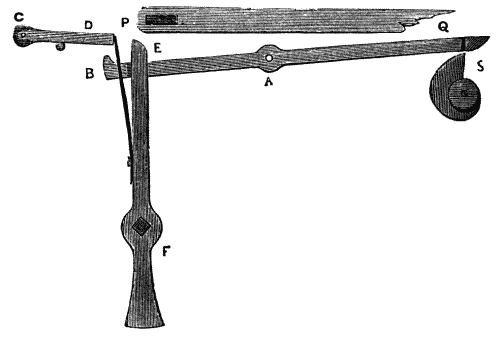
\includegraphics[width=\textwidth]{images/fig53.png}
\label{fig53}
\end{figure}
%-----File: 276.png--------------------------------------------
%-----Folio: 261-----------------------------------------------
certain to overcome any friction there can be between the
two stopping pieces. The lever $\mathrm{BAS}$ drops every quarter
of an hour; but it does nothing except when the stopping
piece is resting against the second stop, \textit{i.e.}, when the
clock has given warning for the hour. It is let off at
the 58th second, or the last beat but one of the pendulum
in the hour, and the train just gets far enough into motion
to let the hammer fall as the seconds hand makes its last
jump for the hour, and it acts with the greatest precision.

This precision in letting off the hour-striking made the
want of it disagreeably apparent in the quarters, which were
at first discharged in the usual way by a snail on the hour
arbor which leads off to the dial work; and we had to put a
larger snail for them on a separate arbor under the escapement
wheels, free from the shake of the hands and dial
work; this answers very well and there is never more than
$2$~seconds difference now in the time of discharging the
quarters. The 1st, 2nd, and 3rd quarters all begin to strike
at those times respectively; but the 4th quarter is let off
about $20$~seconds before the hour so that it may have done
striking before the hour begins at the real time.

That, by the bye, is an objection to a train remontoire let
off at the usual half-minute intervals, viz., that it makes the
interval between the quarters and the hour disagreeably long,
if the hour is to begin striking exactly at the hour as it should
do. Even $20$~seconds is too long an interval for any but very
large bells. However since the invention of these gravity
escapements train remontoires may be considered extinct,
as they cost much more, and are no better, and are almost
certain to be destroyed, or at least put out of action.

\subsection[Winding of striking parts.]{Winding of striking parts.}\markright{WINDING OF STRIKING PARTS.}\label{subsec:Winding_of_striking_parts.}\index{Westminster clock!striking parts!winding of}---Each of these takes about
$5$~hours to wind, and requires double multiplying wheels,
which are as to size repetitions of the large wheels and
pinions of the train, with a modification of the shape of
teeth, which will be explained afterwards, because different
%-----File: 277.png-----------------------------------------------
%-----Folio: 262--------------------------------------------------
shapes are proper for driving and for driven teeth, though
that is very seldom attended to. The striking parts wind
twice a week; for although they might have been made to
go a week, the weight would have had to be twice as
much---and more, on account of the increased friction; and a
man could not have wound up each of them in an ordinary
working day. Moreover the whole work must have been
heavier and larger and had a greater strain upon it. Even
in much smaller clocks than this I always design the striking
parts to go less than a week. I do not believe that there
is a clock in the world that strikes a large bell, say above a
ton weight, \textit{properly}, with winding once a week; unless it
happens to have an unusually large fall for the weights.

There were various \index{Westminster clock!striking parts!curious suggestions for winding}suggestions made both publicly and
privately for winding the clock by water, by a steam engine,
and even by a kind of weighbridge or sinking platform to be
worked involuntarily by people walking over Westminster
bridge, which would have to rise between every two walkers
to do any good: a turnstile would have been a much more
practicable thing. I forget whether anybody proposed to
turn the tide to account for the purpose, but I daresay they
did. It never occurred to these inventors that the interest
on the cost of construction and the expense of looking after
any such machine would far exceed the wages of two
winding men for five or six hours twice a week.

In most large clocks the winding pinion simply `pumps'
out of gear with the winding wheel on the front end of the
barrel, and it does not much signify if it is left in, as the
friction caused by it is not much. But this would not
do for a pair of large wheels, and there was not room to
make the great winding pinion pump out of gear. Moreover
it was absolutely necessary to have some contrivance for
automatically stopping\index{Winding stops!for clocks} the winder a little before every
striking of the part he is winding; which occurs in no other
clock, as none takes anything like a quarter of an hour to
%-----File: 278.png---------------------------------------------
%-----Folio: 263------------------------------------------------
wind either part, and if it did you need only slip off the
handle. That is managed thus. In each striking part a
long lever (omitted in the frontispiece to avoid confusion)
stands in the way of a tooth or arm on the winding arbor:
when the man begins to wind he must lift this lever up on
to a certain hook which will hold it up so long as the weight
of the lever rests upon it; but when the weight is relieved
the hook falls back: this is done by the snail a few minutes
before the clock is going to strike, and just a minute before
it strikes the snail lets the lever drop again, and the hook
being then out of the way, it drops completely and \index{Stops for weights}\index{Turret clocks!stops against overwinding}\index{Weights, stops!for winding}stops the
winder; and he then throws the winding-wheels out of gear,
and in again when the striking is done.

This throwing out of gear is also done by a new method:
the first pivot of the second (150) winding-wheel arbor is set
in an eccentric bush, which can be turned in its own holes
by a lever with a handle to it, as you see in the drawing,
and the eccentricity is just enough to take the teeth of that
pinion out of gear with the great winding wheel, leaving the
2nd wheel in gear with the winding-pinion (14). Besides
this the ropes themselves stop the winder when the weights
are wound up to the top, by throwing another lever off a
hook on which it has to be set before the man can begin
winding. In all these winding and maintaining power
contrivances there are some further provisions for enabling
the man to turn the winding handle back a little, to let the
barrel ratchets down softly on to their clicks, but it is
hardly worth while to describe them.

\subsection[Rate.]{Rate.}\markright{RATE.}\label{subsec:Rate.}\index{Gravity escapements!rate of some}\index{Rate!of the Westminster clock}\index{Westminster clock!rate}---Provision is made in the clock for reporting its
own rate of going to the Greenwich observatory at any convenient
hour or hours every day, by electric telegraph, as I
have already described under `electrical clocks' at p.~\pageref{subsec:Electrical_clocks};
and it has been arranged by the Astronomer Royal that it
should give two signals a day, at an hour before and after
noon, for greater accuracy. The average performance of the
%-----File: 279.png---------------------------------------------
%-----Folio: 264------------------------------------------------
clock is reported by him annually to the Board of Visitors
of the Observatory, and for years the report has been practically
the same. Last year, 1881, its error was under $2$~sec.\ on
$84$~per~cent.\ of the days of observation; between $2$ and
$3$~sec.\ on $14$; between $3$ and $4$ on $2$. They were almost
exactly the same in 1872.

Sir G.~Airy sent me, for the purpose of the inquiry into
the barometrical error (see p.~\pageref{barerr}), the complete rating of
the clock for 1872, except Sundays and a few odd days.
Rejecting three abnormal disturbances, one of which reached
$8$~sec.\ in a week of thunderstorms, and two others of $5$~sec.,
which came suddenly, and evidently from something done in
the clock-room, because the daily variations never reached
$2$~sec.\ at any other time, the average daily variation was only
$0.2$~sec.\ on each side of zero, or $0.4$~sec.\ altogether; and taking
it on all the Saturdays in the year, the average weekly variation
was just $1$~sec, or exactly half that of one of old Mr.~Dent's
best regulators which I happen to have had for
nearly two years while we were trying the Exchange clock.
Therefore the first blow of the hour may be presumed to
differ considerably less than a second from GMT, and is
practically always right within $2$~seconds. In hearing it at
a distance you must allow nearly $5$~seconds a mile for the
velocity of sound.

Some enemy set afloat the statement that the clock is
`controlled' by electrical connection with Greenwich, in
some such way as is described at p.~\pageref{jones}, instead of merely
reporting its own performance; and the story has been repeated
by people who ought to have known better, or might
easily have learnt, by writing either to the Astronomer Royal
or me, or from any edition of this book after the first.
A signal is sent back from Greenwich at some hour daily, for
the information of the winding men, but they never touch
the pendulum unless the error is $2$~seconds, which happens
very seldom.
%-----File: 280.png---------------------------------------------
%-----Folio: 265------------------------------------------------

\subsection[History of the clock.]{History of the clock.}\markboth{HISTORY OF THE CLOCK.}{HISTORY OF THE CLOCK.}\label{subsec:History_of_the_clock.}\index{Westminster clock!history}---It is no longer necessary to
relate as fully as in 1860 the history of the 16 years of
disputes relating to this clock; for it was the subject of
violent disputes before I\index{Beckett, Sir E.!plan for the Westminster clock|(} had anything to do with it. I shall
only say as much as may possibly be useful with reference
to any similar transaction hereafter. Not that I expect
such warnings to be attended to, except perhaps in exactly
the wrong way; for I know very well that the tendency of
the official mind to get things done with as little trouble as
possible is infinitely stronger than to get them done as well
possible. I was only brought into this business originally
with the view of saving somebody else trouble; and as soon
as it was found that by the legal effect of the contract I had
real power to direct the work, every possible effort was made
to get rid both of it and me. No official who joined in
those attempts cared three half-pence how the clock was
made. Luckily I did care, and knew what would become
of it if I gave it up. And as the biographers of Sir Charles
Barry have told their story on his behalf, I shall also, without
the least resentment against them, repeat mine, of which
not a word has been ever contradicted.

No \markright{EARLY DISPUTES ABOUT THE WESTMINSTER CLOCK.}one who has read in the Parliamentary papers the
early correspondence, beginning in 1844, can have the
smallest doubt that the architect had made up his mind
that the late Mr.~Vulliamy\index{Vulliamy, Mr.!and the Westminster clock} should make the clock, and no
one else. Mr.~Vulliamy himself was so confident about it,
that even after the Astronomer Royal had utterly condemned
his plan for it, as `only suitable for a large village clock,'
and recommended old Mr.~Dent\index{Dent, E.~J.!Westminster clock|(}, he said to me, `Dent will
never make that clock.' After that, the matter went to sleep
till November 1851, when the Duke of Somerset, then Lord
Seymour and First Commissioner of Works, asked me to
act as referee with the Astronomer Royal, on his recommendation.
I examined the plans at the Office of Works, which
had been sent in in 1846, and found that Vulliamy's was
%-----File: 281.png--------------------------------------------
%-----Folio: 266-----------------------------------------------
quite as deficient in strength (for which Sir G.~Airy had
commended it) as it was in all provisions for accuracy:
indeed more so, because accuracy is a question of degree;
but such a clock as that, striking on a bell of half the weight
that had been fixed upon, would have destroyed itself in
week. By some strange omission, Dent had never been
told that the bell was to weigh $14$~tons, and he had assumed
it to be much less, and consequently his plan was defective
too, though not so defective, and that only in size, not
in principle. The plans of Whitehurst, of Derby, which
Sir G.~Airy\index{Airy, Sir G.~B.!conditions for Westminster clock} had reported on more favourably than Vulliamy's
could not be found in the office; and it was evident that
Dent's had been somewhere else, where they had been very
roughly handled, dirtied, torn, and mended, which was
certainly not done at Greenwich.

Whitehurst was dead, and Vulliamy had refused to accept
the Astronomer Royal's conditions as to the performance of
the clock, which the Clockmakers' Company also pronounced
impossible, though they have been far exceeded in accuracy
now. So we agreed that it was useless to apply to any one
but Dent, and that the only practicable way was to ask him
if he would make for any definite sum such a clock as we
should require, from his own knowledge and our information
as to what was intended, and such general plan as we could
give him, in the unfinished state of the tower. He agreed to
do so, for a sum which was soon found to be inadequate, and the
arrangement was altered into his keeping a separate account
of all outlay on the clock, and receiving $10$~per~cent.\ profit on
it, which ultimately came to \pounds 4080, only an eighth more than
Vulliamy's\index{Vulliamy, Mr.!and the Westminster clock} estimate for a clock totally unfit for the work.

The Duke of Somerset went out of office soon after giving
Dent the order in 1852; and then began, and lasted through
the reigns of his successors, Lord John Manners and Sir W.~Molesworth,
a series of intrigues and attempts to get rid of
or alter old Mr.~Dent's contract, and then to repudiate his
%-----File: 282.png--------------------------------------------
%-----Folio: 267-----------------------------------------------
successor F.~Dent, and then---or rather, all along---to get
rid of me; for they all knew very well that for various
reasons the Dents alone could not contend against them, nor
go on with the work at all. Sir C.~Barry demanded working
drawings of the clock from Dent, who told him very truly that
there were none, and would be none, except such sketches as
I might give his men from time to time. Then he applied to
the Astronomer Royal for them, who desired me to make and
send them. I answered that I should do nothing of the
kind: the Office of Works might show him the signed plans
if they liked (as in fact they did), which were all that could
possibly concern him; at any rate I should make no others.
Thereupon Sir G.~Airy resigned; and as his knowledge of
large clocks was purely theoretical, and not one of the
suggestions he had made could be adopted, his resignation
saved a good deal more of unprofitable correspondence. The
Office of Works made that another excuse for trying to get
rid of me, and went so far as to consult the Attorney and
Solicitor General about it.

Then they tried the obstructive policy of refusing any
information about the tower, in spite of my warning that
the only consequence would be that they would probably
have to pay for altering the clock when it got there; for
which they cared nothing, as the nation and not they would
have to pay for it. Still the work went on, and as the
inscription on it records, the clock was made in 1854, and
after going in the factory for 5 years was fixed in the tower
in 1859, and was set going permanently in 1860.

Sir C.~Barry\label{barryhands} was particularly anxious to design the hands,
and I rather unwillingly and with some misgiving consented,
having already reason to put very little faith in his
mechanics. He first produced some cast iron ones, of
such frightful weight that I would not even let them be put
on. He then tried some of gun-metal, which were lighter,
but still far too heavy for the clock, besides being so fixed
%-----File: 283.png--------------------------------------------
%-----Folio: 268-----------------------------------------------
on by his engineer that they fell over a minute or two every
time they passed the vertical. And so we removed them,
at least the minute hands, and made new ones, as described
at p.~\pageref{whands}, which have always gone quite easily, except once
when loaded with snow which froze upon a partial thaw,
and broke down hundreds of miles of telegraph wires at the
same time that it stopped the clock. Before Dent's final
bill was paid, the Astronomer Royal inspected the work,
though his legal control over it was gone, both from his
resignation, and from other causes, and he candidly expressed
his entire approval of it, and especially of the escapement,
on which its performance chiefly depends. It is due to Lord
Llanover, though he is dead, to say that in his time I had
no trouble with the Office of Works.

As soon as it was finished, Mr.~W.~Cowper Temple\label{ctemple}, who
had then been made First Commissioner of Works by Lord
Palmerston his step-father, told the House of Commons, with
evident satisfaction, and the gratitude natural to some people,
that my connection with the clock had ceased, and that it
was handed over to the Astronomer Royal. The next I heard
of it was that he had replaced the great check spring of the
hour-striking part by a contrivance of his own, which soon
produced a smash, and then the old spring was quietly
restored, and is there now, and there have been no more
such experiments. I must however do him the justice to
say that he had previously written to me `that the clock
would be far better in my hands than in any other person's;'
not that there was really any more for me to do, beyond
nominal superintendence of the clockmakers who have the
care and winding of it by an independent contract, viz., the
successors of the Dents\index{Dent, E.~J.!Westminster clock|)} in the Strand. By an odd coincidence,
I had the pleasure of giving a sort of clinical lecture
on the clock to as many members of the Horological Institute
as the room would hold, on the 21st anniversary
of our signing the plans for it, 29 January 1873.\index{Beckett, Sir E.!plan for the Westminster clock|)}
%-----File: 284.png--------------------------------------------
%-----Folio: 269-----------------------------------------------




\section{THE WESTMINSTER BELLS.}\label{sec:THE_WESTMINSTER_BELLS.}\markboth{THE WESTMINSTER BELLS.}{HISTORY OF THE WESTMINSTER BELLS.}

\index{Westminster bells, the!their history}
I had better give the history of them also here. In 1852
Astronomer Royal declined to have anything to do
with the bells, as he did not profess to understand them;
and nothing was done towards getting them, beyond
some abortive correspondence with me by Sir W.~Molesworth,
and his giving a commission to Sir C.~Barry and Professor
Wheatstone to learn what they could about bells at the Paris
Exhibition of 1855, which proved to be nothing. In 1856,
Sir B.~Hall (Lord Llanover) asked me to take them in hand,
and it was then arranged that I, with Sir C.~Wheatstone, and
the late Rev.~W.~Taylor\index{Taylor, Rev.~W.!and the Westminster bell}, who had paid some attention to the
subject in a theoretical way (and must be distinguished from
his namesake the bell-founder), should be the referees.
Sir C.~Wheatstone never acted, beyond telling us the
result---or rather, no result---of his inquiries at Paris, and Mr.~Taylor
would take no responsibility beyond giving the final
certificates. I therefore prepared a specification, which was
sent to the three English bell-founders.

Mr.~Mears\index{Mears, bell-founders} refused to accept the referees because they had
among them spoken ill of his two condemned Royal Exchange\index{Mears, bell-founders!Royal Exchange and York}
peals, of his great York Minster bell, and a rather larger
one which he had sent to Montreal. He also declared that
nobody else could make the bells; and his tender was not
the lowest. Mr.~Taylor's (of Loughborough) was; but he
wanted some terms which could not be acceded to. Messrs.~Warner\index{Warners, bell-founders}
required the referees to take the responsibility of
giving the patterns for the bells; \textit{i.e.}, they confessed that
they did not know how to make such large bells of the
proper notes: they had previously copied all their bells from
existing ones. However I was able to do that for them, and
so their tender was accepted, though they demanded ten
guineas a cwt., while the usual price was seven, and they
were to recast any of them (unless condemned for bad
%-----File: 285.png--------------------------------------------
%-----Folio: 270-----------------------------------------------
casting, in which case they were to recast for nothing) for
\pounds 2 a cwt., and also to cast any small experimental bell
the same price.

They made the great bell first; and from some mismanagement
it came out thicker than the pattern, and two tons
heavier than was intended, and required a clapper twice
heavy as we had reckoned on by analogy to other bells.
Undoubtedly we had a right to reject it; but it appeared a
sound casting, except some holes at the top, and was generally
praised by the public who heard it, though there was always
something unsatisfactory in its tone. And no wonder; for
after being rung occasionally for some weeks, it one day
cracked, no doubt from the weight of the clapper which it
required to bring out its tone, and when it was broken up
there was found a great flaw in it, where the two streams of
metal meeting round it had never joined. So we were in
every way well rid of Big Ben\index{Big Ben of Westminster!the first and second} the first.

The founders however had cast then the fourth quarter
bell of four tons successfully, and there was no intention of
taking the job out of their hands. But they demanded a
price for recasting enormously beyond the \pounds $2$~per~cwt.,
which they had agreed to before, evidently presuming that
neither of the other founders would be employed. Mr.~Mears
had learnt something by experience, and no longer objected
to the referees, and offered to recast the bell at a more
reasonable price, and so this time his tender was accepted.
He however was still more unlucky; for he produced a
bell which partially cracked also, after a few months striking;
and Dr.~Percy\index{Percy, Dr., his report on the Westminster bell} pronounced it, on cutting a hole down to the
bottom of the crack, and analysing the metal, `a defective
casting, porous, unhomogeneous,' and at the place where it
is cracked, not of the composition I had prescribed, and
therefore much more brittle.

Mr.~Mears also determined to conceal this porosity from
the referees by filling up the holes with cement, before he
%-----File: 286.png--------------------------------------------
%-----Folio: 271-----------------------------------------------
let us know that the bell was ready to be seen. And when
I publicly charged him with having done so, he put a bold
face on the matter, and brought an action for libel, and had,
no doubt, found half-a-dozen engineers and brass-founders
ready to swear that porous castings are as good as sound
ones. But he also found that I had got a piece\label{taster} of the bell
analyzed, and knew that the composition was wrong, besides
the porosity and its concealment. So his counsel accepted
his costs without a verdict, after making a speech in which
he confessed and declared that the composition had miscarried,
and become unhomogeneous; that he had filled up
the holes, \textit{because he thought them immaterial}---as if he was to be
the judge of that; and that it was impossible---\textit{i.e.}\ that he
did not know how---to cast large bells without holes in them!

His successor, who had bought Mears's declining business,
twenty years afterwards thought he would try again, evidently
with the object of advertising himself, on my once more
publishing the fact that Big Ben II\index{Big Ben of Westminster!the first and second}.\ was a disgrace to its
founders. His workmen who had been with Mears had to
confess the concealment of the holes, and again they and all
his party asserted that it is impossible to cast large bells
without holes, and that it was their regular practice to fill
them up with cement coloured with bell dust: which both
Taylor and Warner's people utterly contradicted, and I have
every reason to believe, quite truly.

Though Dr.~Percy had been asked to examine the bell as soon
as the cracks were discovered, he was not allowed by Mr.~Cowper
Temple, then First Commissioner of Works, to cut into
it for nine months after. If that had been done at once, as I
desired, Mears's action would never have been heard of.

He had also got a report from Sir G.~Airy\index{Airy, Sir G.~B.!his report on the Westminster bells}\label{gairyreport}, who, although
he declined meddling with the bells before because he did
not understand them, felt no difficulty in giving judgment on
them afterwards, with the help of two musical assistants and
fiddle `tuned to the pitch of the Italian opera'---as if the
%-----File: 287.png--------------------------------------------
%-----Folio: 272-----------------------------------------------
pitch of the Italian opera had anything to do with the
question whether five bells are good or bad, or in tune with
each other. Mr.~Turle, the organist of Westminster Abbey,
had given his opinion before we certified them, that the four
quarter bells were `all that can be desired, both in tune and
tone,' which are very different things (for a set of iron pots
may be in tune), except that `the fourth is a shade too flat'
But Sir G.~Airy came to a very different conclusion, viz.,
that the fourth bell was \textit{a note and a half too sharp}, and the
first about the same, the third `rather sharp,' and the second
alone right. On the whole, he was `much dissatisfied with
those bells,' and thought two at any rate must be recast\index{Airy, Sir G.~B.!failure of his alteration of the striking work}.
Afterwards he began to have a little misgiving about it, and
thought it might be advisable to try again before recasting
them; but he never did try again. I suppose it had then
occurred to him, as a mathematical fact of which he certainly
was not ignorant, that the two bells could not be a note
and a half too sharp without being a sixth less in diameter
than they are, or else a great deal thicker. He also
pronounced the great bell, which Dr.~Percy had not then
ascertained to be cracked three inches deep, and to have
almost every possible unsoundness, `perfectly sound for all
practical purposes, and the cracks probably superficial,' and
that it only wanted a lighter hammer \textit{faced with tin!}

This seems to have been too much even for Mr.~Cowper\label{ctemple2}
Temple to swallow; for although he sent me one of the
polite and intelligent epistles which I used to receive from
him and Mr.~Alfred Austin, then the secretary of that office
saying that he `disagreed with every word of the stricture
I had sent him on Sir G.~Airy's report' (as if his adoption
of it made it less ridiculous), he afterwards consulted
Mr.~Turle again, and no quarter bells were recast, nor was
the great hammer faced with tin; and after getting Dr.~Percy's
report he told the House of Commons that the bell
was, not `perfectly sound,' but `irretrievably cracked,' as it
%-----File: 288.png--------------------------------------------
%-----Folio: 273-----------------------------------------------
is, though the defect is much less perceptible than one would
expect. The hours were struck on the fourth quarter bell
for three years, which made them difficult to distinguish at
a distance, and after a paragraph in the \textit{Globe} to that effect,
the striking was resumed on the great bell with a lighter
hammer striking in a different place, which was easily done
by my arrangement for turning the bell any degree round by
giving it a mushroom or button-shaped top (see p.~\pageref{fig44}).
When the new great bell of St.~Paul's has taught people the
difference between a cracked bell and a sound one, perhaps
`this great country' and `the model legislature of the world,'
as it is the fashion to call them, may screw up their courage
to the vast undertaking of recasting their own great clock bell
at the cost of six or seven hundred pounds.

The cost\label{cost}\index{Westminster bells, the!their cost}\index{Westminster clock!cost} of the bells, including \pounds 750 for recasting `Big
Ben' was under \pounds 6000, while the cost of the iron frame
provided by the architect was about \pounds 6600 partly in consequence
of its being made too weak at first, so that it shook
under every blow of the hammers, as I had told him that it
would. And as the clock, with my hands, cost only \pounds 4080,
while his hands and dials alone cost \pounds5334, you see that
the actual clock and bells cost much less than the architect's
appendages to them.




\section{TEETH OF WHEELS.}\label{sec:TEETH_OF_WHEELS}\index{Teeth of wheels}
\markboth{TEETH OF WHEELS.}{TEETH OF WHEELS.}

There are various treaties on this subject, and I only
intend to say as much on it as it is necessary that a clockmaker
should understand, if he means his wheels and
pinions to run together smoothly instead of wearing themselves
out by jerking and scraping, which I have known to
happen in a very few years. The most comprehensive view
of the whole theory of tooth-drawing (at least of this branch
of the art) is in a paper by Sir G.~Airy\index{Airy, Sir G.~B.!on wheel teeth} in the 2nd vol.\ of
the \textit{Cambridge Transactions}, and it was further expanded by
Professor Willis in his \textit{Principles of Mechanism}.
%-----File: 289.png-----------------------------------------------
%-----Folio: 274--------------------------------------------------

Some persons have a mistaken impression that the object
to aim at in constructing wheel-teeth is to make them roll
on one another without any rubbing friction. This can
indeed be done by what are called \textit{involute} teeth, of the
shape described by a point in a string unwound off the
circumference of a wheel: but they are really useless
because they are so oblique that they produce a squeezing
pressure between the two wheels which is more than
equivalent to any saving in friction. The great thing to
aim at in describing teeth is to make the relative velocity of
the wheels uniform from the beginning to the end of the
contact of each pair of teeth, which of course involves also
the absence of all concussion or drop of the teeth. Another
point is to have the action entirely or chiefly between the
teeth which are separating from each other, and not between
those which are approaching, which is commonly expressed
by saying that the action should be after the line of centres
of the wheels and not before it. The reason of this will be
evident at once if you draw some teeth with a very rough
outline, so as to give an exaggerated view of the effect of
friction, for you will see that there is a degree of roughness
which will make the teeth jam against each other and not
let them slide at all as they approach the line of centres,
but that no degree of roughness will do this when they are
leaving contact or are past the line of centres. The most
perfect thing is when the contact takes place for a very
short distance only close to the line of centres; and this
can only be with very small teeth, and therefore very high
numbers (except with involute teeth, which I have already said
will not do for another reason). There is indeed a contrivance,
which I have somewhere seen called White's\index{White's gearing} gearing, for
getting this kind of action with large teeth in heavy machinery,
by putting several large-toothed wheels close together,
with the teeth of each a little behind the other, as in figure~\ref{fig54}~$a$
(next page): but this is never used in clockwork.
%-----File: 290.png--------------------------------------------
%-----Folio: 275-----------------------------------------------

\subsection[Helix-teeth.]{Helix-teeth.}\markboth{HELIX-TEETH.}{HELIX-TEETH.}\label{subsec:Helix-teeth.}\index{Helix teeth}\index{Teeth of wheels!helix teeth}---A modification of this plan, though very
unlike it in appearance, has been occasionally used in
clocks under the erroneous name of the \textit{helix lever}. The
teeth certainly do at first sight suggest the idea of an endless
screw, but are essentially different, the arbors
being parallel, and not at right angles as in an endless
screw. If you suppose a good many very thin toothed
wheels put together side by side, each with its teeth a little
behind its neighbour, they will present a surface like a
rough tooth with a sloped face, as in the upper part of \hyperlink{fig54}{this
figure}~$a$. Then go a step
farther and suppose the
rough edge to be smoothed
off, and the result will be
a smooth-faced oblique
tooth, like the lower one
in the figure, which will
drive teeth of corresponding
obliquity on another
wheel, and the contact will
be solely at the line of
centres, where there is no
friction. But when the
teeth thus become smooth,
there will evidently be a
great endway pressure on
each arbor, which there is
not while the teeth are square, or belonging to separate
wheels put together. This endway pressure may however
be neutralised by again putting two such wheels together
with the teeth sloped opposite ways as at $b$. There was a
German turret clock on this plan in the 1851 Exhibition,
which certainly went with a very small weight; and small
clocks with the single helix tooth had been made in England
many years before by Macdowall (see p.~\pageref{macd}) which also
\begin{figure}[hbtp]
\centering
\hypertarget{fig54}{\caption{\sc Helix Teeth}}
\includegraphics[width=0.6\textwidth]{images/fig54.png}
\label{fig54}
\end{figure}
%-----File: 291.png--------------------------------------------
%-----Folio: 276-----------------------------------------------
required less force than usual, from the smallness of the
friction in the teeth. I do not know that the advantage is
worth the expense; but as this construction is very little
known, I explain it in case it may be turned to any use
hereafter.

\subsection[Epicycloidal teeth.]{Epicycloidal teeth.}\markboth{EPICYCLOIDAL TEETH.}{EPICYCLOIDAL TEETH.}\label{subsec:Epicycloidal_teeth.}\index{Epicycloidal teeth}\index{Teeth of wheels!epicycloidal teeth}---It may be said without exaggeration,
I believe,
that all the teeth
now used in machinery
are constructed
either
as \index{Hypocycloid and epicycloid}epicycloids or
hypocycloids,
and the meaning
of those words is
this:---If you roll
a circle $\mathrm{AGP}$
\textit{on} another circle
$\mathrm{ARY}$, the curve
$\mathrm{RP}$ traced by
any point $\mathrm{P}$ in
the rolling circle
is called an epicycloid
to the circle
$\mathrm{ARY}$; and
if you roll the small circle $\mathrm{AGP}$ \textit{within} a larger than
itself, such  as  $\mathrm{AQX}$, the curve $\mathrm{PQ}$ traced by $\mathrm{P}$ is a
hypocycloid to that circle. And it is remarkable that
if the tracing circle is exactly half the size of the one in
which it rolls, the hypocycloid $\mathrm{PQ}$ is a straight line, and
part of the diameter of the large circle, and therefore teeth
so described are called radial teeth.
\begin{figure}[hbtp]
\centering
\setlength{\unitlength}{0.05\textwidth}
\caption{\sc Epicycloidal Teeth}\index{Teeth of wheels!epicycloidal teeth}
\begin{picture}(16,16)(-8,-2)
\put(0,0){\line(0,1){7}}
%Circle centre (0,3) radius 3
\qbezier(0,0)(1.242641,0)(2.121320,0.878680)
\qbezier(0,0)(-1.242641,0)(-2.121320,0.878680)
\qbezier(2.121320,0.878680)(3,1.757360)(3,3)
\qbezier(-2.121320,0.878680)(-3,1.757360)(-3,3)
\qbezier(0,6)(1.242641,6)(2.121320,5.12132)
\qbezier(0,6)(-1.242641,6)(-2.121320,5.12132)
\qbezier(2.121320,5.12132)(3,4.24264)(3,3)
\qbezier(-2.121320,5.12132)(-3,4.24264)(-3,3)
%Circle centre (0,7) radius 7
\qbezier(0,0)(2.899496,0)(4.949747,2.050253)
\qbezier(0,0)(-2.899496,0)(-4.949747,2.050253)
\qbezier(4.949747,2.050253)(7,4.100507)(7,7)
\qbezier(-4.949747,2.050253)(-7,4.100507)(-7,7)
\qbezier(0,14)(2.899496,14)(4.949747,11.949747)
\qbezier(0,14)(-2.899496,14)(-4.949747,11.949747)
\qbezier(4.949747,11.949747)(7,9.899493)(7,7)
\qbezier(-4.949747,11.949747)(-7,9.899493)(-7,7)
%Two radii
\put(0,3){\line(3,-1){2.846050}}
\put(0,7){\line(2,-3){3.882901}}
%Arc (2pi/7) of circle centre(0,-17) radius 17
\qbezier(0,0)(3.880139,0)(7.376024,-1.683529)
\qbezier(0,0)(-3.880139,0)(-7.376024,-1.683529)
%Curve PR, $\mathrm{R}$ chosen approximately, $\mathrm{Q}$ used as angle point
\qbezier(2.846050,2.051317)(3.882901,1.175649)(3.9,-0.453399)
%Curve PQ, with angle point chosen approximately, on the line OQ
\qbezier(2.846050,2.051317)(3.482901,1.775649)(3.882901,1.175649)
%Labels
\put(0,-0.2){\makebox(0,0)[t]{A}}
\put(0,7.2){\makebox(0,0)[b]{O}}
\put(-2.8,3){\makebox(0,0)[tl]{G}}
\put(6.8,7){\makebox(0,0)[tr]{X}}
\put(2.646050,2.051317){\makebox(0,0)[tr]{P}}
\put(3.882901,1.1){\makebox(0,0)[tl]{Q}}
\put(3.9,-0.6){\makebox(0,0)[t]{R}}
\put(7,-1.8){\makebox(0,0)[t]{Y}}
\put(0,13){\makebox(0,0)[t]{\it Runner}}
\put(0,-2){\makebox(0,0)[l]{\it Driver}}
\put(2,-2){\vector(1,0){2}}
\end{picture}
\label{fig55}
\end{figure}
Now suppose $\mathrm{ARY}$ is the circumference of what is called
the \textit{geometrical} or \textit{pitch} circle of a wheel which is intended
to drive another, and $\mathrm{AQX}$ the pitch circle of the wheel to
%-----File: 292.png--------------------------------------------
%-----Folio: 277-----------------------------------------------
be driven, which is generally called the `follower,' but
which I think it better to call the \markboth{TEETH OF WHEELS.}{TEETH OF DRIVER AND RUNNER.}\textit{runner}, as followers do
not usually run before their driver; then it is easy to see
that the arc $\mathrm{AP}$ of the tracing circle is equal both to $\mathrm{AR}$
and to $\mathrm{AQ}$, and also that the epicycloid is always more
convex than the hypocycloid, and therefore that the point
$\mathrm{P}$ in the tracing circle is always the point of contact
between two teeth so traced, and the velocity of the two
wheels is always the same as if their pitch circles rolled
upon each other without any teeth at all; and therefore
it is constant in all positions of the teeth. It is hardly
necessary to observe that the teeth of the driver, to act
after the line of centres, must be wholly outside its pitch
circle, and those of the runner wholly within. The part
of a tooth within the pitch circle is generally called its
\textit{flank} or \textit{root}, and the part outside is called the \textit{point}, or
the \textit{addendum}, and sometimes the \textit{curve}, because the flank
is generally made radial, \textit{i.e.}\ a hypocycloid described by a
circle of half the diameter of the pitch circle. For it is
further to be observed, that although the points of the
driver and the flanks of the runner must be traced with
the same circle, it is not the least necessary that the
points and the flanks of the same teeth should be traced
with the same circle.

In clockwork the wheels always drive and the pinions
run, except the $12$~hour wheel in the dial-work, and the
winding wheels and pinions if there are any. It can be
proved, as you may see in Professor Willis's\index{Willis, Prof., his table of wheelwork} \textit{Principles of
Mechanism}, but the proof is too long to give here, that no
pinion of less than $11$ leaves (except of a kind which I
shall describe presently) can be driven entirely after the
line of centres. A pinion of $10$ can very nearly; and there
is so much difference between the force required to drive
pinions of $8$ and those of higher numbers, that some
spring clocks with Macdowall's escapement which answered
%-----File: 293.png--------------------------------------------
%-----Folio: 278-----------------------------------------------
perfectly with pinions of $10$ or $12$, failed with the common
pinions of $8$, for want of force to drive the two extra wheels
in the train. Professor Willis gave the \hyperlink{willis}{following} table of
the lowest numbers which will work together with all the
action after the line of centres:---

\begin{table}[!hbtp]
\centering\hypertarget{willis}{}
\setlength{\tabcolsep}{4pt}
\begin{tabular}{lrrrrrrrrrrrrrrr}
Driver &54 &30 &24 &20 &17 &15 &14 &13 &12 &11 &10 &9  &8  &7  &6 \\
Runner &11 &12 &13 &14 &15 &16 &17 &18 &19 &21 &23 &27 &35 &32 &176
\end{tabular}
\end{table}
\begin{figure}[hbtp]
\centering
\caption{\sc Drivers and Runners}
\includegraphics[width=324pt]{images/fig56.png}
\label{fig56}
\end{figure}

The practical inference from this is, that if you use these
numbers, or any higher ones, together, the driving teeth\index{Driving and running teeth}
require no flanks and the running ones no points: indeed
if you mean to prevent any action before the line of centres,
the runners obviously must have no points, because if they
have they will be geometrically identical with the teeth of
a pinion intended to drive the wheel after the line of centres
when reversed. Suppose for instance, what is nearly the
case in the Westminster clock, that the great striking wheel
at one end of the barrel and the great winding wheel at the
other are both of the same size and number of teeth, and
%-----File: 294.png--------------------------------------------
%-----Folio: 279-----------------------------------------------
that their pinions are also the same; then as the striking
wheel always drives, but the winding wheel is always driven
by its pinion, the striking pinion and the winding wheel
ought to have no points to their teeth, and the sections
of the two wheels and pinions would be as in fig.~\ref{fig56}, the
right hand representing the striking part and the left the
winding, and the action being in both cases, you observe,
after the line of centres $\mathrm{AC}$, as the arrows indicate.

It is evident that the same wheel cannot properly drive
two unequal pinions with radial teeth. Whenever the
same wheel has to drive two such pinions, the flanks of
the pinion teeth and the points of the wheel teeth must be
traced with the same circle, and that circle must not be
larger than half the size of the smaller pinion, or else it
will make the teeth of that pinion weaker at the roots
than even radial teeth are, which are of course narrower at
the bottom than the top, and therefore are a weak form,
especially in small pinions. A case of this kind occurs in
every clock on the patterns I have described at pp.~\pageref{fig37} and
\pageref{fig40}, and in the Westminster clock, and in short wherever
the second wheel in the going train does not turn in an
hour, and the dial work is driven independently. In this
case, the $40$ teeth of the hour wheel (or whatever the number
may be) require no points, and should be hypocycloids
described by a tracing circle of half the diameter of the other
pinion of $10$ or $12$ which is driven by the great wheel, if the
teeth of that pinion are radial.

\subsection[Lantern pinions.]{Lantern pinions.}\markboth{LANTERN PINIONS.}{PROPER USE AND CONSTRUCTION OF LANTERN PINIONS.}\label{subsec:Lantern_pinions.}\index{Lantern pinions for clocks|(}\index{Pinions of clocks!lantern}\index{Teeth of wheels!lantern pinions}---But there is another, perfectly
different kind of pinion, which is much better for small
numbers than radial teeth or leaves, viz.\ what is called
a lantern pinion, and in old books, a `trundle.' These two
figures~(\hyperlink{fig57}{\textit{t.~o.}}) will show its construction better than any explanation.
I believe it is the oldest form of pinion in the
world, but it had almost (if not quite) fallen into disuse in
England, when it was restored in Dent's turret clocks about $30$
%-----File: 295.png--------------------------------------------
%-----Folio: 280-----------------------------------------------
years ago. They work with much less friction than common
leaved pinions of low numbers, when driven, the run upon
them being less and the action wholly after the line of
centres, and the shape of the wheel teeth requiring less
accuracy to drive them smoothly. They are not however
proper for driving, because then you see the action comes
all before the line of centres. In some French turret clocks
the winding pinions are nevertheless wrongly made as
lanterns, and the pins themselves pivotted instead of
\begin{figure}[htbp]
\centering
\hypertarget{fig57}{\caption{\sc Lantern Pinions}}
\includegraphics[height=357pt]{images/fig57.png}
\label{fig57}
\end{figure}
%-----File: 296.png--------------------------------------------
%-----Folio: 281-----------------------------------------------
rivetted in their sockets so as to turn while they are working,
which makes the working loose and shaky and the
pinion itself very much weaker than when the pins are fast,
and saves very little in friction besides.

For the purpose of geometrical construction, we may first
consider the pins as being of infinitely small thickness, and
then the teeth which drive them would be of the dotted form
$\mathrm{PR}$ fig.~\ref{fig57}, being epicycloids traced on the wheel with a
circle the full size of the pitch circle of the pinion. Then in
order to get the shape of the teeth for pins of the actual size,
you must gage off half the breadth of the pin from each side
of the tooth, which reduces it to $pr$ and you may leave on
just as much point as will keep hold of the departing pin $\mathrm{P}$
until another tooth has got well hold of the next pin just as
it crosses the line of centres. This operation of reducing the
theoretical to the actual tooth is practically equivalent to
tracing the tooth with a smaller circle: how much smaller,
will depend on the number, \textit{i.e.}\ on the thickness, of the pins,
in proportion to the size of the pinion. I find that a lantern
of $8$ or $10$ requires a tooth which fits a leaved pinion of the
same number so nearly that I can see no difference in the
curves on a pattern as large as $9$~inches diameter; and even
with $12$ the difference is very small; although a theoretical
lantern pinion with pins of no thickness requires the same
shape of teeth as a radial pinion of twice its size. I have no
doubt that a lantern of $8$ runs as easily as a leaved pinion of
$12$, and of course it requires only $\frac23$ the number of teeth in
the wheel, and is also itself stronger, and much less liable to
break, both in hardening and in working afterwards.

I may however repeat the caution that cast iron wheels do
not work so well with steel pinions, which lanterns necessarily
are (or rather, they, soon wear them out), as with
cast iron; and therefore if the great wheel only is of iron and
the smaller ones of brass or gun metal, the pinions should be
made of cast iron\index{Cast iron!for steel pinions} or steel accordingly. Also it should be
%-----File: 297.png--------------------------------------------
%-----Folio: 282-----------------------------------------------
borne in mind that you cannot draw out an arbor with a
lantern pinion endways, by unscrewing the front bush only
and therefore they should not be used where you cannot conveniently
get at the back bush to take it off. These pinions
are used in all the American clocks and also in the cheap
German or `Dutch' clocks, both of which, it is well known,
will go with an amount of dust in their insides which would
stop a clock with leaved pinions completely. But the English
clockmakers will not use them in small clocks; and as
English small clocks are not yet made in factories as large
ones are, and as they are everywhere else in the world, the
men who make them up have the power of obstructing every
such improvement, and exercise it by immediately charging a
higher price for every deviation from the common form, or
for everything which they fancy is going to be applied to some
new use.

The leaved\index{Leaved pinions}\index{Pinions of clocks!leaved}\index{Teeth of wheels!leaved pinions}\markboth{LEAVED PINIONS.}{LEAVED PINIONS.} pinions of English house clocks are made out
of `pinion wire,' which is in fact a very long pinion drawn
through a hole like wire, and the leaves are turned off to form
the arbor and pivots (see p.~\pageref{pivots}). The American and Dutch
clocks prove clearly enough that lantern pinions\index{Lantern pinions for clocks|)} can be made
at least as cheap as others; and if any man of skill, capital,
and determination would follow the example of Mr.~Hobbs in
locks, and set to work to manufacture clocks in a factory of
his own, we should soon see this and other improvements
made, and the clock trade recovered out of the hands of
foreigners, to whom it has been in a great measure sent away
by this combination of workmen, who will ruin this and every
trade in the kingdom if they are allowed to have their own
short-sighted way.

Inasmuch as English clocks are thus made by hand, and
therefore probably no two are exactly alike, it is necessary
to have a tool for marking the places where the holes for the
pivots of the wheels are to be drilled, to bring them to the
proper depth for working. This \textit{depthing tool}\label{depthing}\index{Depthing tool@`Depthing' tool described}\markboth{DEPTHING TOOL.}{DEPTHING TOOL.} is something
%-----File: 298.png--------------------------------------------
%-----Folio: 283-----------------------------------------------
like two vices framed together parallel to each other, each
carrying a thick sliding pin sideways through each of its
jaws. These $4$ pins have a small hole or `centre' at the
inner end and a point at the outer. The pivots of the pair
of wheels to be fitted are put in the $4$ centred ends of the
pins, and the machine is adjusted by trial till the wheels are
felt to work together comfortably. Then the points at the
outer ends of each pair of pins indicate the distance of the
centres of the wheels, and may be used to mark that distance
on the frame-plate. If you cannot get two wheels to work
together without shake (so long as they are driven the same
way) by any adjustment of their depth, the teeth are wrongly
cut in one of them at least, and they have no business to be
used.

\subsection[Internal wheels]{Internal wheels}\markboth{INTERNAL WHEELS.}{INTERNAL WHEELS.}\label{subsec:Internal_wheels}\index{Teeth of wheels!internal wheels}\ are wheels with the teeth turned inwards
in which case the rim must evidently be raised in a
different plane from the spokes. They are never used in
clock-work, except for some special purpose, such as Sir G.~Airy's
maintaining power in the Exchange clock (p.~\pageref{smallmaintain}) or
in a sun and planet wheel for the same purpose, neither of
which are desirable, and in some train remontoires (p.~\pageref{fig48}).
Whenever they have to be used they are best made with pins
driven into the flat rim, especially if they have to be driven
and not to drive. Otherwise the same rules apply to the
construction of internal teeth as to external ones. They
almost necessarily involve the fixing of the wheel or pinion
which works into them on a stud instead of on an arbor
with pivots, which is generally objectionable and ought
never to be allowed if it can be helped, either for wheels or
pulleys.

\subsection[Bevelled wheels.]{Bevelled wheels.}\markboth{BEVELLED WHEELS.}{BEVELLED WHEELS.}\label{subsec:Bevelled_wheels.}\index{Bevelled wheels}\index{Teeth of wheels!bevelled wheels}\index{Wheels for clocks!bevelled}---When the direction of motion has to
be changed, as it often has in leading off to dial-work in
turret clocks, bevelled wheels are used (as shown in p.~\pageref{fig47}).
They may be made to act through any other angle just as
well as $90^\circ$. The only condition to be satisfied is that the
%-----File: 299.png--------------------------------------------
%-----Folio: 284-----------------------------------------------
teeth should in every respect converge to the point where
the two arbors would meet if prolonged, as if they were on
the faces of two cones. Nevertheless in a great many bevelled
wheels, the sides of the teeth do not converge properly,
the spaces being made of the same width all along, and so
the teeth converge too much, and have no contact at all
except just at their outer edges. The reason of this is that
if the sides of two adjacent teeth are cut in the common way
with the same cutter, the breadth of the cut is the same
throughout, and not narrower at the inside than the outside,
and therefore the teeth evidently taper too much. Fortunately
there is seldom much pressure on the bevelled
wheels in clocks, and therefore the defect is not very
material: but still it is one, and its frequent occurrence is
another reason why the bevelled wheels should be large in
diameter rather than in thickness; for the larger they are
the less pressure there is on the teeth, and the less any
inaccuracy of cutting is felt (as it is in wheels of all shapes),
and also the less shake of the hands and wheels there will
be for any given amount of shake in the teeth.

\subsection[Skew-bevelled wheels.]{Skew-bevelled wheels.}\markboth{SKEW-BEVELLED WHEELS.}{SKEW-BEVELLED WHEELS.}\label{subsec:Skew-bevelled_wheels.}\index{Skew-bevelled wheels}\index{Wheels for clocks!skew-bevelled}---It may be worth while to know
that bevelled wheels can be made with oblique teeth, to work
with their arbors not in the same plane, provided they have
only to work one way; but the friction is very great if they
work what may be called the wrong way, and even in the
right way the friction is more than in the usual conical
wheels. I have never myself seen any clock where it was
necessary to resort to this construction, which may be found
in books on machinery, and therefore I only mention it in
case anybody may have occasion to resort to it.

\subsection[Cams]{Cams}\markboth{CAMS TO RAISE LEVERS.}{PROPER FORM OF CAMS.}\label{subsec:Cams}\index{Cams}\index{Teeth of wheels!cams}\ may be defined as teeth which have to raise a lever,
or a sliding rod, and not a succession of teeth, and therefore
each cam must work up to its end, and drop the lever there,
whereas in wheels a second pair of teeth may and always
should come into action before the preceding pair have quite
%-----File: 300.png-----------------------------------------------
%-----Folio: 285--------------------------------------------------
separated. The simplest form of cams to raise a lever is
that shown in any of the pictures of striking work of house
clocks, figs.~\ref{fig33} to \ref{fig36}, viz.\ a set of pins stuck into the side of
a wheel which catch the lever at some distance from its end
and work up to the end and then let it drop off. This does
well enough for very light hammers requiring only a small
clock weight, but is the worst plan that could be invented
for large ones. If you take the trouble to draw a wheel with
$8$ pins in it, each pin acting on the lever through about $36^\circ$
(leaving the difference between that and $45^\circ$ for the clearance)
you will see that the angular lift of the lever towards the end
of its motion is only one third of what it is at the beginning,
and therefore $\frac23$ of the clock weight is wasted during part of
the lift. And that is by no means all; for if you look at
p.~\pageref{fig43} you will see that, as turret clock hammers are usually
fixed, the weight of the hammer acts more vertically or
requires more force to lift it at the beginning of its motion,
where the pin has least leverage or power, than at the
end, where it has most; and besides all this, the loss of
power by friction in driving through short levers is much
greater than through long ones with less angular motion.
Under all these circumstances it is no wonder that the weight
required to make a large clock strike is often three or four
times the theoretical `duty' of the clock, or the equivalent
of the hammer $\times$ its lift $\times$ as many blows as it strikes for
once winding; \textit{i.e.}\ that $\frac23$ or $\frac34$ of the force is wasted in
bad leverage and friction: whereas in the Westminster striking
part little more than $\frac14$ of the theoretical duty of the
clock weight is lost in friction, leverage, and the necessary
clearance or drop for the lever.

The first condition therefore which the striking cams
ought to satisfy is they should begin to act at the end of the
lever. It is not necessary that the action should be quite at
the end all the way through, provided it is so at the beginning,
where the lift is hardest for the clock, and at the end
%-----File: 301.png--------------------------------------------
%-----Folio: 286-----------------------------------------------
of the action so as to let the lever drop suddenly; for which
reason also rollers are worse than half round pins, besides
the reasons just now given against using pins at all. The
curve which does keep the cam\index{Cams!proper form of}\index{Teeth of wheels!cams!construction of} acting on the end of the
lever throughout, and as a tangent to itself, without any
scraping, is called in mathematics the \textit{tractrix}. If you wish
to describe it, the way is this. Set a smooth round board of
the size of the cam wheel with stiffish paper pasted over it
(to efface the grain of the wood) on a pin through the centre
on a horizontal table; and set also on the table, on another
pin, a model of the intended lever, with a vertical pencil at
its intended point, so as to press upon the paper, the lever
being weighted a little. Set the lever on the line of centres
and turn the wheel; it will drag the pencil over its surface
in a curve which is the \textit{tractrix}\index{Tractrix curve, to describe for cams}, unless it has been disturbed
by some inequality of friction between the paper and the
pencil, or at the axis of the lever; which is so likely to
happen that you cannot safely rely on this construction,
unless you find that a good many of the curves so traced
agree with each other.

It\label{camcalc} fortunately happens however, that there is an epicycloid
which agrees with this so nearly that it may be
used without sensible error. Suppose $r$ is the radius of
the circle which forms the bottom of the cams (\textit{i.e.}\ their
theoretical pitch circle, allowing nothing for clearing the end
of the lever) and $l$ the length of the lever. The lever will
work as a tangent on its end throughout (without any appreciable
error for such length of cam as is ever wanted) on
epicycloidal cams traced with a circle whose $\normalfont{diameter}
=\sqrt{r^2+rl}-r$. Thus if $r=8$~in.\ and $l=4$~in.\ the radius of the
tracing circle will $=.95$~in. Another advantage of these
cams is that you may cut them off at any length, provided
only you keep the lever of the proper length; if you alter
that you will get scraping friction, and soon wear out either
the cams or the lever.
%-----File: 302.png--------------------------------------------
%-----Folio: 287-----------------------------------------------

\markright{MODES OF TRACING CAMS.}If you prefer having circles to deal with instead of epicycloids,
there is another form of cam, which was suggested to
me by Mr.~Effingham Lawrence (another horological lawyer,
like Mr.~Bloxam, and all the members but one of that jury
in the 1851 Exhibition, both English and foreign), and which
acts quite as well as the epicycloid or tractrix, provided you
take care not to alter the length of the cam: \textit{i.e.}\ you must
not put more or fewer cams on the wheel than they are
designed for, and you must take care that the proper distance
of centres of the wheel and lever is preserved. In
fig.~\ref{fig58}, $\mathrm{CAL}$ is the line of centres, and $\mathrm{AB}$ the space for
one cam on their pitch circle; by which I mean the space
occupied in lifting, for you see a little space is left below the
line of centres before the next cam begins, to prevent the
lever dropping onto the cam itself, which shakes the clock
most injuriously. $\mathrm{AP}$ is the arc of the lever. Draw $\mathrm{AT}$,
which is a tangent to the two circles at $\mathrm{A}$, and $\mathrm{BT}$ a tangent
\begin{figure}[htbp]
\centering
\caption{\sc Modes of Tracing Cams}
\includegraphics[width=\textwidth]{images/fig58.png}
\label{fig58}
\end{figure}
to the cam circle at $\mathrm{B}$\@. That point $\mathrm{T}$ will also evidently
be the place where a tangent to the circle $\mathrm{AP}$ at $\mathrm{P}$ would
meet the others; or in other words, $\mathrm{T}$ is the centre of a
circle $\mathrm{BP}$, to which the lever itself will be a tangent both at
the beginning and the end of the lift, although the contact
%-----File: 303.png--------------------------------------------
%-----Folio: 288-----------------------------------------------
will be a little way from the end during some intermediate
part of the action. The backs of the cams must be cut out
a little deeper than down to the pitch circle, to let the lever
drop freely; and it is important to remember that the end of
the lever itself should not be left sharp, or it will cut off the
ends of the cams if they are not very hard, and perhaps break
them if they are. I know that by experience.

It does not occur to me that cams can ever be required in
clock-work for lifting a vertical rod sliding like a stamper.
If any such case should occur, involutes of the wheel circle
would be the right shape for the cams.\footnote{This is no exception to the epicycloidal rule, for an involute is
in fact an epicycloid traced by a circle of infinite size, \textit{i.e.}\ by
a straight line.} There may also be
cases where it would be worth while to pull down a long
striking rod by pins in the wheel catching a square hook at
the end of the rod, and dragging it on with a little sideway
motion until it is struck off the pins by a horizontal stop:
this would avoid all the lever work and all friction except at
the striking off of the hook.

\subsection[Oil for clocks.]{Oil for clocks.}\markboth{OIL FOR CLOCKS.}{OIL FOR CLOCKS.}\label{subsec:Oil_for_clocks.}\index{Oil for clocks}---I believe it is now generally understood
that sweet oil is the worst that can be used for machinery,
large or small, except when it is purified in certain ways not
known to the public; and then it is too expensive for use in
large or common clocks. For them purified sperm oil, such
as is now made wholesale for other machinery, is quite good
enough. Common neat's-foot oil may also be purified into
a very good oil, which will hardly freeze here. It can only
be done in cold weather; it should be shaken in a bottle
with water until it becomes a thick white soup, and then
left to stand, and the fine oil that gradually comes to the top
skimmed off, taking care to get none of the thick. If it is
done in a warm temperature, oil appears at the top as fine,
which has no business there, and will not remain fine in
cold weather.
%-----File: 304.png--------------------------------------------
%-----Folio: 289-----------------------------------------------

I have found two advantages in using the animal and
sperm over vegetable oil, which some persons may be
glad to learn. Working in iron with the common olive oil
dirties your hands so that it is very difficult to clean them,
whereas animal or sperm oil helps to clean them. It also
preserves iron from rust far better and longer, and does not
turn green on brass, \textit{i.e.}\ does not produce verdigris. I
understand that petroleum is better still for preventing rust.
It is difficult to make amateur clock-cleaners understand or
remember that putting oil to pinions driven by brass or gun-metal
wheels wears them out; but this does not apply to
cast iron; and all pivots should be oiled, and acting surfaces
generally. Oil must never be put to the beat pins of a
gravity escapement, or it will make them stick to the
pendulum quite enough to affect its rate; but it should be to
the pallet pivots. I have known the want of it, both there
and in the common pallet pivots, affect the arc sensibly.

It must be remembered that oil has always a tendency to
run away from small points of teeth, the ends of pins, \&c.,
to the thicker parts of the wheel. In some French clocks
the teeth of the dead scapewheel are accordingly made with
a kind of lump at the end; but this wastes more space in
the clearance or drop, and it is never done in English clocks,
so far as I have seen; nor do I know anything that will
answer---except putting on fresh oil when it is wanted. Dirty
oil should always be cleaned off before putting fresh oil on.
When it has got very thick it sometimes requires soda in
warm water to remove it.
%-----File: 305.png--------------------------------------------
%-----Folio: 290-----------------------------------------------




\chapter{WATCHES AND CHRONOMETERS.}\label{chap:WATCHES_AND_CHRONOMETERS.}
\phantomsection
\addcontentsline{toc}{section}{Watches and Chronometers.}

The early history of watches\label{History_of_early_watches}\index{Watches!their early history} is no less obscure than that
of clocks, though many centuries later. Tradition assigns
the invention to the town of Nuremberg, in the fifteenth
century. According to a once famous book, Derham's
`Artificial Clockmaker,' of 1714, and Beckmann's `History
of Inventions,' they appear to have existed in the time
of our Henry VIII., and of Louis XI., of France, and
especially of the Emperor Charles V., who used to keep
many watches going, as near together as he could. Erasmus
had a watch given him by a Polish nobleman, early in the
sixteenth century. And by Queen Elizabeth's time they
had become pretty common, and are alluded to by Shakspeare
in \textit{Twelfth Night}---`I frown the while, and perchance wind
up my watch.' The London Company of Clockmakers was
incorporated in 1631; and not long after that, the invention
of the spring balance, the distinctive element of watches,
was contended for between Huyghens\index{Huyghens!theory of balance-spring for watches} and Dr.~Hooke\index{Hooke, inventor of the balance-spring of watches}, who
both claimed the invention of the pendulum for clocks
(see p.~\pageref{huyghens}). It seems clear that Hooke first enunciated
the discovery of the isochronism of springs in the short
sentence, \textit{Ut tensio sic vis;} or the force varies as the degree
of tension: which rule however we shall see presently has
two rather curious exceptions.

\subsection[The main-spring]{The main-spring}\markboth{MAIN-SPRINGS.}{MAIN-SPRINGS.}\label{subsec:The_main-spring}\index{Mainspring of watches}\index{Watches!mainspring}\ of a watch is a thin ribbon of steel
coiled up in a barrel round a strong spindle, to which one
end of the spring is fixed, the other end being fixed to the
barrel. When it is wound up the coils lie close together
upon the spindle or arbor, and as the spring runs down, the
coils separate from the arbor, and lie close to the barrel.
The simplest construction, still used in most of the foreign
%-----File: 306.png---------------------------------------------
%-----Folio: 291------------------------------------------------
watches, is for the barrel arbor to be the winding arbor,
having a ratchet wheel squared onto it, held by a click on
the frame or plate of the watch, and the great wheel is on
the barrel itself; and in this case, as I explained at p.~\pageref{folio_145},
with reference to spring clocks, no temporary maintaining
power `going\index{Maintaining powers of clocks or going barrels!going-barrel in watches} barrel' is required to keep the watch going
while you are winding it up. But it is obvious that as the
force of the spring is greater when it is tightly wound up
than when it is loose, the force of the train will be very
far from constant throughout the day, although that may not
affect the going of the watch from one day to another. On
the other hand, there is found to be a very singular exception
to that rule of Dr.~Hooke's, stated just now, inasmuch as
there is a position of the spring coiled in a barrel in this
way, in which there is no material variation of its force for
a few turns. And certainly some of the foreign watches
made in this way go very well.

Even if a watch does go rather faster at one time of the
day than another (which it is not certain that such watches
do), it is of no consequence, provided they go uniformly
from day to day; and there has been strong testimony
published in the \textit{Horological Journal}, that they do, when
well made, of course. I have seen watches with tapered
main-springs (though the foreign ones are not tapered), in
which you could not perceive any difference in the force, by
the usual testing apparatus of a weighted lever, whether
the spring was wholly wound up or not. And if this is
so, the addition of any more machinery, being superfluous,
is mischievous, and only increases the expense and size of
\begin{figure}[!htbp]
\centering
\caption{\sc American Main-spring Barrel}
\includegraphics[width=0.6\textwidth]{images/fig59.png}
\label{fig59}
\end{figure}
the watch, and risk of the chain breaking, perhaps the most
common of all accidents. There is evidently a tendency
in watch-making now to dispense with such machinery, except
for marine chronometers, which are required to go uniformly
at all times of day, and not merely from day to day.
Accordingly, both in Switzerland and America, which are
%-----File: 307.png---------------------------------------------
%-----Folio: 292------------------------------------------------
gradually stealing away our common watch trade, as well as
that in many kinds of clocks, the fusee and chain (which I
will describe presently) are almost universally omitted.\index{Fusee of watches!often dispensed with}

\begin{wrapfigure}{o}{155pt}
\centering
\caption{\sc American Watch}
\includegraphics[height=500pt]{images/fig60.png}
\label{fig60}
\end{wrapfigure}

But in that case there is another risk of breaking, for
when the spring breaks, the barrel recoils violently from
the sudden removal of the pressure, and often breaks some
teeth of the great wheel fixed upon it. Partly to avoid
this, and also for general improvement in strength and
arrangement of the train, the American\label{uswatch}\markboth{AMERICAN MAIN-SPRING BARREL.}{AMERICAN MAIN-SPRING BARREL.} watches\index{American clocks!watches}, as made
by the \index{Howard@`Howard Clock Company,' of America}`Howard Company,' under a patent by a Mr.~Reed
of 1857, have the spring contained in an immovable barrel\index{American clocks!mainspring barrel},
which  is a solid part of the upper plate of the frame
(calling the dial side the
lower). The outer end of the
spring hooks to the barrel as
usual, and the inner end to
the winding arbor, on which
the great wheel rides, with a
spring maintaining power, just
like those of a clock described
at p.~\pageref{subsec:Harrison's_going_barrel}. For safety
also, the main-spring is held
by two clicks, much stronger
than the single one generally
put into fusee watches, and the maintaining spring is also
very strong. Fig.~\ref{fig59} is a plan of this, and fig.~\ref{fig60} a
section of the whole watch. It may be observed also that
a watch of this kind turns the same way in winding as
one with a fusee, whereas the common foreign watches turn
the opposite way: not that there is any real importance in
this, except that the absence of uniformity sometimes causes
people to wind a new watch forcibly the wrong way.

To prevent that, Breguet invented what is called the tipsy
key\index{Breguet's tipsy key}\label{tipsy}\index{Tipsy winding-key}\markboth{TIPSY WINDING KEYS.}{TIPSY WINGING KEYS.}, not that that adjective belongs to the `winder,' in the
clockmaker's sense of a key, but in the more human sense.
%-----File: 308.png---------------------------------------------
%-----Folio: 293------------------------------------------------
The handle is connected with the pipe by a pair of ratchets,
which would be called \textit{clutches} in large machinery, which
which can pass each other one way, but not the other; and they
are kept together, and then hardly visible, by a spiral
spring, which gives way, and lets one pass over the other
if the handle is turned the wrong way.
The best shape for a winding key\index{Key!best watch}\index{Watch keys, best kind of}\index{Winding keys!for watches} is
like a pencil with a rough handle, to
enable you to twirl it more easily
between your fingers. You thereby
apply less force, and are less likely to
do mischief by wrong, or over winding;
and moreover you keep the watch
steady, instead of turning it in your
left hand, and agitating the balance at
every turn.

If you compare figure~\ref{fig60} with \ref{fig61},
you will see that in the latter, which
is the common English fusee and chain
watch, the third wheel of the train
has to be sunk in the plate below the
centre wheel, whereas in the American
watch (fig.~\ref{fig60}) it stands free and
clear. There are a few other things in
this arrangement which had better be
postponed till other parts of the watch
have been described, and we will
proceed with the description of the
common English watch construction,
and therein first of the

\subsection[Fusee.]{Fusee.}\markboth{FUSEE.}{ENGLISH WATCH MOVEMENT.}\label{subsec:Fusee.}\index{Watches!fusee}\index{Fusee of watches}---That piece is a hollow-sided cone, which you
see in this picture of a chronometer or English watch movement,
with a chain round it and the barrel, and the
great wheel is no longer on the barrel, but on this conical
piece called the fusee. When the spring is wound up
%-----File: 309.png---------------------------------------------
%-----Folio: 294------------------------------------------------
and its force is greatest, the chain acts on the small end
of the fusee, and therefore with the smallest leverage; and
as the spring unwinds, the chain acts on a thicker part of
the fusee, and it can be, and in good watches is, so adjusted
that the force on the train and escapement is constant. It
was suggested by Mudge\index{Mudge!invented the lever escapement for watches}, the inventor of the lever escapement
in the form now used in 99 out of 100 English\index{English fusee watch}
watches, that the usual position of the chain is wrong: and
so it is; for you see in fig.~\ref{fig61}  that it acts on the opposite
side of the fusee to the centre pinion, and consequently the
pressure and friction on the fusee pivots (which are necessarily
large ones) is the \textit{sum} of the force of the spring on the
fusee and of the great wheel on the pinion; whereas if the
\begin{figure}[htbp]
\centering
\caption{\sc English Fusee Watch}
\includegraphics[width=\textwidth]{images/fig61.png}\index{Watches!general construction}
\label{fig61}
\end{figure}
%-----File: 310.png---------------------------------------------
%-----Folio: 295------------------------------------------------
spring acted on the same side as the pinion, it would only
be the \textit{difference}. I confess I know no reason why the
common arrangement should be adhered to, except that it is
the common one, which is generally considered reason enough
for anything bad.

The train of wheels\index{Train of wheels!in watches}\index{Wheels, numbers of teeth!in watches} in a watch is much the same as in a
clock except that the scapewheel is not the wheel which
turns in a minute and carries the second hand, but is another
faster wheel. In a pocket lever watch the balance generally
beats in $2$-$9$ths of a second, and in a chronometer\index{Chronometers} either in that
time or in $\frac14$~sec. The scapewheel generally has $15$ teeth,
and therefore turns in $6$~seconds, or something near it. In
a good lever watch the pinions are generally $7$, $8$, $8$, $10$, and
the wheels $63$, $60$, $64$, $75$; in a pocket chronometer the
pinions are $8$, $10$, $10$, $12$, and the wheels $80$, $75$, $80$, $72$; in
box\index{Box chronometer} or marine chronometers the numbers are still higher, the
pinions being $10$, $10$, $12$, $14$, and the wheels $80$, $80$, $90$, $90$.
Box chronometers are generally made to go rather more than
$2$~days, though they are wound up every day, and they have
a small hand on what is called the `up and down' circle in
the dial, indicating how far the barrel has run down. In
these watch trains it must be observed that where a slow
wheel has fewer teeth than a quick one, the teeth must be
larger, or the wheels could not be put into the frame. I
think no pinion so low as $7$ should be admitted, and I cannot
understand why $9$ should be a prohibited number in clocks
and watches, as it seems to be, or at any rate was until I
introduced it frequently in turret clocks.

Common watches have the balance above the upper plate.\index{Watches!general construction}
What are called \textbf{three-quarter plate}\index{Three-quarter plate watches} watches have a large
piece of that plate cut away, and the balance lies about level
with the rest of the plate, and most of the wheels have their
upper pivots in cocks screwed to the lower plate. This
saves thickness in the watch.

\subsection[Winding stops.]{Winding stops.}\markboth{WINDING STOPS.}{WINDING STOPS.}\label{subsec:Winding_stops.}\index{Stop, winding, of watches}\index{Watches!winding-stops}\index{Winding stops!for watches}---A watch, or a spring clock, with a
%-----File: 311.png---------------------------------------------
%-----Folio: 296------------------------------------------------
fusee, is stopped from being overwound by a long tooth which
you see in fig.~\ref{fig61}, sticking out from the thin end of the
fusee. There is a spring lever with a hook fixed to the
frame with a little play on its pivot, so that when the chain
comes to that end, or the fusee is full, it pushes the lever
just far enough for its hook to catch the tooth, and so stops
the winding. In foreign watches without a fusee, a thing
called the \textit{Geneva stop}\index{Geneva stop}\index{Stop, Geneva} is used: it consists of a small wheel
on the barrel-arbor, with only one tooth in it, and the rest
of the circumference filled up blank; this tooth works into
the teeth of another loose wheel, with the hand on it in
fig.~\ref{fig62}, which has only as many teeth as the turns that the
barrel has to make in winding, and has also a blank space in
its circumference. The one-toothed wheel turns the loose
wheel through the space of one tooth for every turn of
the barrel, and when those teeth are all past, the one-tooth
jams against the blank in the loose wheel and lets the barrel
turn no more, and so stops the winding. These two wheels
are above the upper plate. The same thing might be put
on a fusee arbor, but the spring stop is preferred.

\begin{figure}[htbp]
\centering
\caption{\sc Up and Down Dial}
\includegraphics[width=0.7\textwidth]{images/fig62.png}
\label{fig62}
\end{figure}

\subsection[The `up and down dial,']{The `up and down dial,'}\markboth{THE `UP AND DOWN DIAL,'}{THE `UP AND DOWN DIAL,'}\label{subsec:The_`up_and_down_dial,'}\index{Up@`Up and down' dial}\ just now described, on the usual
construction, involves
an additional pair of
wheels. But Mr.~A.~L.~Dennison\index{Dennison, A.~L., of America!his improved Geneva stop} of
America, now settled
here, who is said to
have been the originator
of watch-making
by machinery (which
at last is taking root
here, at Messrs.~Rotherham's well-known
watch factory
at Coventry), patented a modification of the Geneva
%-----File: 312.png---------------------------------------------
%-----Folio: 297------------------------------------------------
stop which enables this kind of indicator to be added without
any more wheels. It consists  merely of adding a short
arbor and hand to the loose or second or star wheel of the
Geneva stop which is applied to watches on the American
plan described at p.~\pageref{uswatch}. These pieces are shown in this
figure~\ref{fig62} of which the right hand part is the plan and the
other the section. This is not of so much value in a
common watch as in a chronometer, but is convenient
to be able to see at a glance whether you have wound
your watch up fully, without the risk of straining it in
trying.

\subsection[The dial wheels]{The dial wheels}\markboth{WATCH DIAL WORK.}{WATCH DIAL WORK.}\label{subsec:The_dial_wheels}\index{Dial wheels!of watches}\index{Watches!dial wheels}\index{Wheels, numbers of teeth!for dials}\ of a watch are more like those of a
turret clock than of a house clock in the division of the
numbers of the teeth, as there is no occasion for the intermediate
wheel called $\mathrm{N}$ in pages~\pageref{fig25}, \pageref{fig34}, to turn in an
hour, as it does in house clocks to discharge the striking,
and even in silent clocks for uniformity. The hand sockets
are also only held on by friction without any spring. In
other respects the train of a watch is substantially the same
as that of a small clock until we reach the escapement, except
that there is one more wheel in the train, for the reason
given just now. The dial pinions in a good watch are $12$
and $14$, and the wheels $42$ and $48$; in a box chronometer
they are $14$ and $18$, and $54$ and $56$.

\subsection[Balance spring.]{Balance spring.}\markboth{BALANCE SPRING.}{BALANCE SPRING.}\label{subsec:Balance_spring.}\index{Balance spring}\index{Watches!balance-spring}---The rest of the machinery of a watch\index{Balance springs of watches}
only differs in size from that of a clock, until we come to the
escapement and the balance. We shall consider the various
escapements presently, but the object of them all is the same
as in clocks, to produce an escape of teeth by the vibration
of a balance, the time of which depends on its own moment
of inertia and a coil of very thin steel wire called the balance
spring, and sometimes popularly the hair-spring from its thinness,
and sometimes (very absurdly) the pendulum-spring,
though it is of the very essence of a pendulum to act solely
by gravity and the essence of a balance to be free from the
%-----File: 313.png---------------------------------------------
%-----Folio: 298------------------------------------------------
action of gravity, or else the `balance' is not balanced and
the watch will go differently in different positions. The
spring by which a pendulum is hung produces no sensible
effect on its time, and is only used to avoid the friction
any other mode of suspension.

The balance-spring is fixed at its outer end to a stud in
the watch, and at its inner to the balance arbor or staff
at the neutral position of the spring the balance is at the
middle of the escape. In some kinds of escapements therefore
the balance cannot stand still if the watch is wound up;
and in all of them the spring tends to bring the balance back
again after it has gone a certain distance, depending on the
force of the escapement and the cleanness of the pivots and
teeth on one hand, and the strength of the spring on the
other, and then the balance swings an equal distance beyond
zero the other way. Whereas in the original clocks with a
balance but no spring (p.~\pageref{sec:BALANCE-WHEEL_ESCAPEMENTS.}) it was only the recoil of the
escapement that brought the balance back again, and such a
balance could not have been used with any kind of dead
escapement, because it would never have returned. Moreover,
considering that a pendulum moves by gravity, through
an arc of only $4^\circ$ or $5^\circ$ with a variation never amounting
to $30'$ in a good clock, while the balance swings independently
of gravity\label{free} through an arc of sometimes $400^\circ$ and
sometimes no more than $100^\circ$, it is evident that a watch
escapement must be a very different thing from that of a
clock.

When I say that a balance is independent of gravity, you
must remember the distinction between mere mass, which
we denoted by the letter $\mathrm{M}$ in treating of pendulums, and
mass acting as a force by means of its weight, \textit{i.e.}\ by the
earth's attraction, which we called $\mathrm{M}g$. The mass and the
moment of inertia of a balance have quite as much to do
with its motion as they have in a pendulum, but the force
which makes it vibrate or return from the impulse given in
%-----File: 314.png---------------------------------------------
%-----Folio: 299------------------------------------------------
the escapement is not gravity, which must be entirely excluded,
for the reason just now given. It was to this
balance spring that Hooke's law of the force varying as the
tension or space moved through (which always implies
\markright{NOT ALWAYS ISOCHRONOUS.}isochronism) was meant to apply, and does apply pretty
generally; but not invariably, because it is found that not
every length of a given spiral spring is quite isochronous, but
only certain lengths, which have to be determined by experiment.

The time of vibration therefore depends on the moment of
inertia of the balance directly and the force of the balance
spring inversely; and in a given spring the force varies
inversely as the length. Consequently you can quicken the
vibration either by reducing the moment of inertia or the
size of the balance, or by shortening the effective length of
the spring. The latter method is used in all common watches,
and the former in chronometers and watches in which extreme
accuracy is aimed at.

\subsection[Regulation]{Regulation}\markboth{REGULATION OF WATCHES.}{REGULATION OF WATCHES.}\label{subsec:Regulation}\index{Regulation!of watches}\index{Watches!regulation}\ of a common watch, to make it go faster or
slower, is done by a lever or index $\mathrm{SPT}$ (fig.~\ref{fig63}), which
turns on a ring set on the watch plate (through which the
\textit{staff} or arbor of the balance has to pass from the inside to
the outside of the watch frame), and it has two small pins at
$\mathrm{P}$ which embrace the spring, one end of the spring being
fixed to the frame at $\mathrm{R}$ and the other end to the balance at
$\mathrm{S}$\@. It is evident that as you turn the regulator to the right
you shorten the length of the acting part of the spring and
so make the vibrations faster, and if you move it to the left,
slower. If the regulator has been moved as far toward \textit{fast}
as it can go and the watch still looses, the spring must
be taken up altogether at $\mathrm{R}$; and then in order that the
balance may still be in the middle position of the escapement
when the spring is neutral, the piece $\mathrm{S}$ by which
it is attached to the balance is itself a ring which fits
tightly round the staff and can be moved when the balance
%-----File: 315.png---------------------------------------------
%-----Folio: 300------------------------------------------------
is taken out, to alter the position and length of the
spring.

\begin{figure}[ht!bp]
\centering
\caption{\sc Regulation of Watches}
\includegraphics[height=300pt]{images/fig63.png}
\label{fig63}
\end{figure}

It must have occurred to everybody who has had to regulate
a good watch for very small errors that there is a want
of some better method than the common one both for moving
the regulator and for seeing how much you move it. Occasionally,
but very
rarely, the index is
made to move by a
tangent screw\index{Timing screws}, turnable
by the watch
key, and I am surprised
that good
watches are not always
made in this
way. But I have
lately seen another,
in the American
watches referred to
at p.~\pageref{subsec:The_`up_and_down_dial,'}, which is
still more delicate,
and also easier to
make. The index
is resisted one way
by a slight spring
fixed to the plate,
and a common screw, in the same direction as a tangent
screw, acts upon it the other way. This avoids the shake
of a tangent screw, and you know that however little you
turn the screw you move the index some distance. In
these cases you must learn by trial how much half a turn
of the screw accelerates or retards the watch per day, and
after that you can regulate it to the utmost nicety---so far
as its errors are amenable to regulation.

Another method suggested by the late Mr.~Dent\index{Dent, E.~J.!regulation of watches} is shown
%-----File: 316.png--------------------------------------------
%-----Folio: 301-----------------------------------------------
in fig.~\ref{fig63}. Instead of being made with a point, the index
has fine bevelled edges lying quite over the index plate,
which is to be made with oblique divisions and two or three
cross lines, like the scale generally engraved on a dividing
rule: this enables the eye to measure much smaller divisions
than could be either seen or cut upon a degree plate of the
common form. But this does not remove the difficulty of
moving it a very little, and the screw is manifestly better.
The old plan\index{Regulation!of watches!the old plan} of a segment of a wheel turned by a pinion
with the index fixed to it
(fig.~\ref{fig64}) is better than
the common one, and I
do not know why it is
disused.
\begin{figure}[htbp]
\centering
\caption{\sc Old Plan}
\includegraphics[width=0.7\textwidth]{images/fig64.png}\index{Regulation!of watches!the old plan}
\label{fig64}
\end{figure}

This mode of regulating
by shortening the
effective length of the
spring is not accurate
enough for chronometers
for another reason, viz.\ that
all lengths of the
spring are not quite isochronous for different arcs of vibration,
and therefore if you have got the spring adjusted
for an isochronous length, it will become unisochronous
if you shorten it a little; and moreover a spring moving
in that way, partly held fast at the ends and passing
loosely through curb pins at $\mathrm{P}$, is not so steady as
one held fast only at the ends. Chronometer balances
are therefore regulated by \textit{timing-screws}, which are screws
with heavy heads set in the rim of the balance: screwing
them in of course diminishes the moment of inertia
and quickens the balance, and vice vers\^a. In chronometers
also the spring is generally made as a cylindrical spiral and
not a flat one. Some chronometer makers have doubted
whether there is any advantage in the cylindrical form, but
%-----File: 317.png--------------------------------------------
%-----Folio: 302-----------------------------------------------
it is now almost universally adopted, and therefore I
suppose the balance of experience is in favour of it. It is
now said that the best form is one that combines both
or a cylinder returned  into a flat spiral both at top and
bottom.

\markright{FORMS OF BALANCE SPRINGS.}But the quality of the spring is probably of more importance
than its form. A medal of the highest class was
awarded in the 1851 Exhibition to M.~Lutz\index{Lutz of Geneva, his balance springs} of Geneva for
some balance springs, made by a secret method, which bore
being pulled out nearly straight, and laid on a hot plate
without suffering any change of form, which was not the
case with any others which were then submitted to us.
I see that aluminium bronze has been successfully used in
Saxony for balance springs\index{Aluminium bronze!balance springs}; but I know nothing more of
them.

\subsection[Glass balance springs]{Glass balance springs}\markboth{GLASS BALANCE SPRINGS.}{GLASS BALANCE SPRINGS.}\label{subsec:Glass_balance_springs}\index{Balance spring!glass}\index{Glass balance springs}\index{Watches!glass balance springs for}.---These were suggested by
Berthoud but have been very little used. The rate of a
chronometer with a glass spring, which Dent sent to Greenwich
many years ago, was very good; and they have the
advantage of varying so much less than steel or any other
metal in elasticity that they require very little compensation
of the balance. I do not know why they have not been more
used, unless it be from the fear of breaking them when anything
is done to the watch\index{Balance springs of watches}. It appears that with them, as
with steel springs, the watch always gains after a new spring
has gone a few months, as if it acquired more elasticity by
working; and this is analogous to what takes place in bells,
which become more sonorous, \textit{i.e.}\ more elastic, after a few
months ringing.

\subsection[Timing for position.]{Timing for position.}\markboth{TIMING FOR POSITION.}{TIMING FOR POSITION.}\label{subsec:Timing_for_position.}\index{Timing screws!timing for position}\index{Watches!timing for position}---As a watch sometimes lies flat on
a table, and sometimes vertical, and not always in the same
position in your pocket, it is necessary that the balance
should keep the same time in all positions, both horizontal,
and with either iii, vi, ix, or xii, upwards. With a heavy
balance it is impossible to get the same arc of vibration when
%-----File: 318.png--------------------------------------------
%-----Folio: 303-----------------------------------------------
\begin{figure}[htbp]
\centering
\hypertarget{fig65}{\caption{\sc Box Chronometer in Gimbals}}
\includegraphics[width=0.6\textwidth]{images/fig65.png}
\label{fig65}
\end{figure}
the watch is vertical and horizontal, because the friction of
the pivots is much greater when they are acting on their
sides than on the point of one of them. If you take a small
chimney-piece clock with a balance and hold it sideways so
that the balance becomes vertical and its staff horizontal,
you will see the vibration diminish very much, and then the
least want of isochronism
in the spring will set the
rate wrong. \markboth{BOX CHRONOMETER IN GIMBALS.}{BOX CHRONOMETER IN GIMBALS.}Marine chronometers\index{Chronometers}\index{Marine chronometer},
which are only
very large watches, are
therefore always set horizontally
in a box, in \textit{gimbals}\index{Gimbals, chronometer},
as in \hyperlink{fig65}{this drawing},
which keep the watch horizontal,
even when the box
is tilted by the ship: if the
box is tilted at $\mathrm{E}$ or $\mathrm{W}$, it
turns on the outer pivots $\mathrm{NS}$ of the gimbal ring, and
if the $\mathrm{N}$ or $\mathrm{S}$ side is tilted, then the box and ring together
turn on the inner pivots at $\mathrm{W}$ and $\mathrm{E}$ leaving the watch
steady. The level of the pivots should be only just
enough above the centre of gravity of the watch to
make it keep its level, for if the c.g.\ is much below the
points of support the watch will swing when they are
moved.

\subsection[Ship time-pieces.]{Ship time-pieces.}\markboth{SHIP TIME-PIECES.}{SHIP TIME-PIECES.}\label{subsec:Ship_time-pieces.}\index{Ship time-pieces}\index{Timepieces, ship}---There is another kind of ship-clocks
made to hang against a wall, not pretending to the accuracy
of chronometers, but a very neat and convenient and cheap
form of time-piece for other places as well as ships. They
are a large $8$-day lever watch with the balance staff and the
scapewheel arbor vertical, and therefore the third wheel in
the train a \textit{contrate} or crown-wheel as at p.~\pageref{crown}. Like other
things, they are of very different qualities with the same
%-----File: 319.png--------------------------------------------
%-----Folio: 304-----------------------------------------------
external aspect. They do not work well without a fusee,
though many of them are made so for cheapness and the
contrate wheel arbor ought to have an end-stop to the pivot
which tends to push away from the scapewheel pinion and
work upon its shoulders, and the two vertical arbors
ought still more to have their lower pivots resting on stops,
either of hard steel or jewels, to take the weight and friction
off their shoulders. End stops are sometimes put to
the horizontal arbors of highly finished clocks; but as there
is no end pressure on them, I think it is hardly worth while
there, though it is in the two cases I have just mentioned.
\markboth{CHIMNEY-PIECE CLOCKS.}{CHIMNEY-PIECE CLOCKS.}Chimney-piece\index{Chimney-piece clocks} clocks with balances (the only ones which
housemaids will allow to go, unless they are too heavy to
move) ought always to have them compensated, for otherwise
the great changes of temperature to which they are
exposed will make it impossible for them to go right, as I
shall now explain.

\section{COMPENSATION OF BALANCES.}\label{sec:COMPENSATION_OF_BALANCES.}\index{Balances, compensation of}\index{Compensation of balances!common}
\index{Watches!compensation of balances}\markboth{COMPENSATION OF BALANCE.}{COMPENSATION OF BALANCE.}
Watch balances, or rather the springs on which their time
depends, vary much more with heat and cold than pendulums,
and therefore compensation is still more essential if you
expect great accuracy of rate; and if it were not that
watches are kept at a pretty even temperature during the day
by near contact with men's bodies, their variations in hot and
cold weather would be enormous: women's watches being
generally worn loose, go worse than men's for that reason.
A small portable clock with a balance uncompensated goes
twenty times worse than the commonest pendulum clock.
The balance itself also expands a little with heat, as a pendulum
does, but the effect of that is small compared with the
variation of the force of the spring. It appears from some
experiments made by Berthoud in 1773, and others by
Dent communicated to the British Association in 1833,
%-----File: 320.png--------------------------------------------
%-----Folio: 305-----------------------------------------------
which nearly agreed, that the loss of time due to expansion
of the balance for a rise of temperature from $32^\circ$ to $100^\circ$ is
not a $5$th of that due to the loss of elasticity and elongation
of the spring, and that the two together amount to no less
than $6\frac12$~minutes a day; and a variation of $33^\circ$ would produce
a variation of an hour in $3$~weeks; whereas we saw that
a common iron wire pendulum would only lose $10$~sec.\ a day
for such an increase of heat, and a wooden one not more
than $1\frac12$~seconds.

The first watch compensation was made by Harrison\index{Harrison!inventor of watch compensation}\label{harrleroy}, who
has been mentioned several times already as the inventor of
various horological improvements; and he received the first
parliamentary reward for improvements in chronometers
with a view to finding longitude at sea. His method is quite
disused now, and indeed he was himself dissatisfied with it,
and suggested that the compensation ought to be done in the
balance and not by any contrivance for altering the effective
length of the spring, which was the principle of his own and
all the early compensations. For this purpose he put the
curb pins ($\mathrm{P}$ in fig.~\ref{fig63} p.~\pageref{fig63}) on a compound bar, of which
one side was made of brass and the other of steel. As
brass expands more than steel, the bar bends to the steel side
when the heat increases, and thus the curb pins were moved
along the spring, as they are by hand in the common regulator.
It is not necessary to dwell on any of the various modifications
of this plan, as they are all now abandoned for the
balance of compound bars, which appears to have been first
made, as well as a mercurial compensation balance, by Julien
le Roy, a celebrated French clockmaker, but afterwards
much improved by the first Arnold, Earnshaw, and various
other English makers. A great variety of these early contrivances
may be found in Rees's Cyclop\ae dia by those who
are curious about them.

The plan\markright{COMMON METHOD.} which is now always used, with some modifications
in certain cases, as I shall explain afterwards, is
%-----File: 321.png--------------------------------------------
%-----Folio: 306-----------------------------------------------
\begin{figure}[htbp]
\centering
\hypertarget{fig61}{\caption{\sc Common Method of Compensation}}
\includegraphics[width=0.5\textwidth]{images/fig66.png}
\label{fig66}
\end{figure}
exhibited  in \hyperlink{fig61}{this drawing}: $tat^\prime$ is the main bar of the
balance, with the timing screws $tt^\prime$ for regulation at the ends;
and $t b, t^\prime b^\prime$ are two compound bars, of which the outside is
brass and the inside steel, carrying weights $b b^\prime$ which may
be screwed on at different places. As the heat increases,
those bars with their weights
bend inwards and diminish
the moment of inertia of the
balance. The only secure
way of making these balances
is to cut them out of a solid
steel disc round which melted
brass is run which \textit{brazes} itself
fast on. This plan of uniting
the metals was introduced by
Earnshaw, it appears, besides
various other improvements
in the construction of chronometers,
in which very little alteration has been made in
nearly 100 years. The principal expense of a really compensated
balance is in the time required for adjusting it,
which can only be done by trial. Many watches are sold
with balances only constructed for compensation but never
adjusted, and therefore under or over compensated, or with
no regularity in the action of the compensation; and some
still worse, with a mere sham compensation, resembling a
compensated balance only in appearance, sometimes not even
cut through.

\subsection[The chronometrical thermometer]{The chronometrical thermometer}\markboth{THE CHRONOMETRICAL THERMOMETER.}{THE CHRONOMETRICAL THERMOMETER.}\label{subsec:The_chronometrical_thermometer}\index{Chronometrical thermometer}\index{Thermometer, chronometrical}\ is simply a watch
with a balance compensated the wrong way, \textit{i.e.}\ with the
brass inside and the steel outside, so as to increase the
retardation from heat and the acceleration from cold. The
use of it is to measure the quantity of heat or cold received
during any given period without recording the actual degree
of heat or cold at any particular time. It is therefore
%-----File: 322.png--------------------------------------------
%-----Folio: 307-----------------------------------------------
used at the Greenwich Observatory for trying the rates of
compensated chronometers under great variations of temperature.

\subsection[Secondary compensation.]{Secondary compensation.}\markboth{SECONDARY COMPENSATION.}{SECONDARY COMPENSATION.}\label{subsec:Secondary_compensation.}\index{Chronometer escapement!secondary compensation}\index{Compensation of balances!secondary}\index{Secondary compensation!theory of}\index{Watches!compensation of balances!secondary}---When chronometers had
brought to great perfection, so as to go with scarcely
any sensible variation of rate while they were kept within
moderate limits of temperature, it was observed that they
always lost if the temperature either rose or fell beyond
those limits; and on the other hand, if the compensation
adjusted for two extreme temperatures, then the watch
always gained at mean ones. I believe it has never
been disputed that old Mr.~Dent was the first person to
explain the cause of this error, in the \textit{Nautical Magazine} in
1833; and he gave the following illustration of it: The
diminution of the force of the spring proceeds uniformly in
proportion to the increase of heat, and may therefore be
represented by a straight line inclined at some angle to
another straight line which is divided into degrees of temperature.
But the inertia of a compound balance such as I have
described cannot be made to decrease quite as fast as the
heat increases; and therefore its rate of variation can only
be represented by a curve, and can only coincide with the
straight line representing the variation of force of the spring
in two points, either the two extremes, or two means, or one
mean and one extreme point: in other words, the compensation
can only be exact for some two temperatures for which
you may choose to adjust it.

The same thing may be shown mathematically\label{2ndmath}\markboth{MATHEMATICAL THEORY OF THE SECONDARY COMPENSATIONS.}{MATHEMATICAL THEORY OF THE SECONDARY COMPENSATIONS.} as follows:
Let $r$ be the distance of the compensation weights from the
staff or axis of the balance, and we may call them both together
$\mathrm{M}$, and for this purpose we have nothing to do with the rest
of the balance. Let $dr$ be the increase of distance of the
weights for some given decrease of heat. Then the new
moment of inertia of the balance will be $\mathrm{M}(r^2 + 2r dr + dr^2)$,
and the ratio of the new inertia to the old will be
%-----File: 323.png--------------------------------------------
%-----Folio: 308-----------------------------------------------
$1+\frac{2dr}{r}+(\frac{dr}{r})^2$; and now the term $(\frac{dr}{r})^2$ is too
large to be disregarded as it may be in the similar formula
for pendulums, because $dr$ must be much larger in proportion
to $r$ than it is in a pendulum, as we have seen already.  Again,
the ratio of the moment of inertia for an equal increase of
heat to its amount of inertia in the middle state will be
$1-\frac{2r}{r}+(\frac{dr}{r})^2$, assuming that equal successive increments
of heat produce equal variations of $r$, which however
is not quite the case, as it is in pendulums. Consequently
the increase of moment of inertia, for a given rise of temperature
is less than its decrease for an equal fall by $2(\frac{dr}{r})^2$, or
the compensation fails to that extent in one of the three
states of cold, middle, or hot temperature.

The correction of this error is called the secondary or
auxiliary compensation, and it is the point to which I think
every chronometer invention for the last thirty-five years
has been directed, chiefly because the chronometers are now
exposed to such extreme and unnatural variations of temperature
in the Greenwich trials\index{Greenwich!trials of chronometers at}---nearly as much as $100^\circ$, that
the attention of the makers seems to be withdrawn from
everything else; and every year's tables display an
increased number of contrivances for this purpose, but
no increased accuracy in the recorded rates of the best of
them.

\subsection[Greenwich trials.]{Greenwich trials.}\markboth{GREENWICH TRIALS.}{GREENWICH TRIALS.}\label{subsec:Greenwich_trials.}\index{Chronometer escapement!secondary compensation!trials at Greenwich}---When the rates of some chronometers
were returned to Greenwich after one of the Arctic
expeditions, the Astronomer Royal reported that they had
been \textit{kept so warm} that they afforded no test of the relative
value of the different modes of compensation employed in
them. I think it might also have been inferred from that
fact that the trials at home in such unnatural variations of
temperature are only calculated to test a single and comparatively
%-----File: 324.png---------------------------------------------
%-----Folio: 309------------------------------------------------
immaterial quality of the chronometers, and to
frighten away from public trial every invention for the
general improvement of the instrument in other respects.
Any nautical man who wants chronometers for real use
would rather have one that would not vary a second a
week in such temperatures as it is likely to be exposed to
in any voyage in a ship's cabin, than one which may possibly
go better than it at some extreme and improbable variation
of temperature, but worse in all ordinary and probable
variations.

Mr.~Hartnupp's report of the trials of above 1000 chronometers
at Liverpool\index{Chronometer escapement!secondary compensation!trials at Liverpool}, in 1872, says that the best of them,
with the ordinary compensation, generally gain $6$~sec.\ a day
more at $70^\circ$ than at $55^\circ$ or $85^\circ$, if the compensation is
adjusted for these two temperatures, and that those which
have the same rate at $55^\circ$ and $70^\circ$, or at $85^\circ$ and $70^\circ$,
lose $1.5$ sec, for a change of $15^\circ$ below or above the
temperatures for which they are compensated. He adds,
that the connection between rate and temperature remains
constant for a long time.

\subsection[Eiffe's compensation balance]{Eiffe's compensation balance}\markboth{EIFFE'S COMPENSATION BALANCE}{EIFFE'S COMPENSATION BALANCE}\label{subsec:Eiffe's_compensation_balance}\index{Compensation of balances!Eiffe's}\index{Eiffe's compensation balance}\index{Secondary compensation!inventions for|(}\ was the first invention
for this purpose which was disclosed; and a reward of 300\textit{l}.\ was
therefore given him by the Admiralty on the recommendation
of the late Astronomer Royal. At the very time while
this invention was under trial at Greenwich, Mr.~Molineux
took out a patent for one precisely similar; which is only
one of the usual proofs that when the time is ripe for an invention,
it is almost sure to be made by several people at once,
of whom one gets rewarded---or suffers, by a patent. Mr.~Eiffe described several methods for effecting the secondary
compensation; the one which he chiefly relied on, and
which has been followed by some other makers, is a balance
in which the compensation bar, or a screw in it, is made to
reach another in the form of a spring with a small weight
upon it, when it has bent inwards to a certain extent, and it
%-----File: 325.png---------------------------------------------
%-----Folio: 310------------------------------------------------
carries that other with it, so as to diminish the moment of
inertia still more than the single compound bar. It seems
an obvious objection to this, that it is discontinuous, \textit{i.e.}, that
the secondary compensation comes into action suddenly at
one change of temperature only. Nevertheless it appears to
answer as well as or better than many others which are free
from that objection.

\begin{figure}[htbp]
\centering
\caption{\sc Dent's Balance}
\includegraphics[width=0.7\textwidth]{images/fig67.png}
\label{fig67}
\end{figure}

\subsection[Dent's balance.]{Dent's balance.}\markboth{DENT'S BALANCE.}{DENT'S BALANCE.}\label{subsec:Dent's_balance.}\index{Compensation of balances!Dent's}\index{Dent, E.~J.!compensation balance}---That objection was obviated in
Dent's balance, of which
also there were several
forms: this is the one which
he proposed as the best
in his pamphlet on the
subject. The flat cross-bar
$rr'$ is itself a compensation
bar with the brass
below and the steel above,
so that if the compensation
weights $bb'$ were set upon
upright stems from the bar
they would be bent in towards
the axis when the
heat increases. But they
are in fact set upon some other bent compensation bars $st$,
$st'$, of which the brass is inside the bend, and consequently
the weights approach the axis more than if they were set on
stems of fixed length; and as they can be set anywhere on
the stems the compensation is thus adjustable. The reason
why the bent bars stand outwards across the principal bar
is to leave room for the balance spring, which is attached
to the smaller cross-bar $d$ shown in fig.~\ref{fig67}, in which
spring is omitted to avoid confusion. This compensation
has the advantage of being continuous.

Loseby's\index{Compensation of balances!Loseby's}\index{Loseby's!balance for watches} balance was an ingenious alteration of a previous
mercurial compensation of Le Roy into this form.
%-----File: 326.png---------------------------------------------
%-----Folio: 311------------------------------------------------
$\mathrm{DD}$ are the weights on the usual compound bars $\mathrm{BB}$, for
the primary or principal compensation. Besides, there are
two small bent thermometers with the bulbs at $\mathrm{F}$, and the
tubes at $\mathrm{E}$, into which the mercury runs as the heat increases,
and so more of the weight of the balance is carried inwards than
is due to the mere bending of the primary bars. The tubes
are sealed with a little air included. $\mathrm{CC}$ are the usual timing
screws independent of the compensation. The action
\hyperlink{fig68}{here} is equally continuous with Dent's, and Loseby's
chronometers generally got a very high place in the Greenwich
lists during the seven years in which he sent them
there; and he would have done wisely to be content with
that success. But he applied no less than four times for a
reward for his invention, and the Astronomer Royal four
times reported against his claim, on the ground that his
balance was neither the first to do what was wanted, nor
was proved to be the best. Mr.~Loseby then sent to the
Admiralty a long memorial, containing a comparison\markboth{LOSEBY'S V. DENT'S COMPENSATION.}{LOSEBY'S V. DENT'S COMPENSATION.} of the
\begin{figure}[htbp]
\centering
\hypertarget{fig68}{\caption{\sc Loseby's Balance}}
\includegraphics[width=0.7\textwidth]{images/fig68.png}
\label{fig68}
\end{figure}
%-----File: 327.png---------------------------------------------
%-----Folio: 312------------------------------------------------
rates of his chronometers with others in the Greenwich lists
for 5 years, to prove that his was the best; and the last
horological paper to which old Mr.~Dent put his hand before
his death was a counter statement, showing that a proper
analysis of those very trials exhibited Loseby's compensation
to be decidedly inferior to Dent's own, and not at
all superior to Eiffe's or several others of which the constructions
were not disclosed.

After his death in 1853 the controversy was carried on in
the Society of Arts' Journal by Mr.~Loseby and me, as he
had assumed that I wrote Dent's paper for him, and so I
extended the analysis to the whole seven years during which
Loseby's chronometers were at Greenwich, and with the
same result. The nature of the analysis is simple enough,
viz.\ this: If you divide the $6$~months of published rates
in each year into $3$~periods, one containing all the coldest
weeks, another all the hottest, and another the mean temperature
weeks---and whether you make the division into equal
periods, or into two periods of $6$~weeks of extreme temperatures,
and $13$ or $14$ of mean, or make it just where the
register shows that the greatest breaks of temperature actually
occurred---the result was always the same, that Loseby's
compensation was the most successful in only one of the
seven years, three other makers' each once, and Dent's three
times. Sir G.~Airy, the Astronomer Royal, was therefore
clearly right in rejecting Mr.~Loseby's claim to a public
reward, whatever may have been his personal skill in
preparing a single chronometer for trial in a year, and so, on
the whole, getting a high place in the list.

\subsection[Kullberg's]{Kullberg's}\markboth{KULLBERG'S COMPENSATION BALANCE.}{KULLBERG'S COMPENSATION BALANCE.}\label{subsec:Kullberg's}\index{Compensation of balances!Kullberg's}\index{Kullberg's!compensation balance}\ compensation balance has been so successful in
the Greenwich trials that I add a description of it to those
mentioned before. The drawing in the \hyperlink{fig69}{next page} shows its
shape, but not the peculiarity of its construction; for the
brass is attached to the top of the cross-bar $\mathrm{AC}$, but to the
bottom of the curved rims $\mathrm{CB}$, the effect of which is that the
%-----File: 328.png---------------------------------------------
%-----Folio: 313------------------------------------------------
ends of the cross-bar are carried downwards by heat, and the
weights $\mathrm{P}$ upwards, and more inwards than if the cross-bar
did not bend, as it does also in Dent's balance; $\mathrm{DD}$
are the timing screws. The principle of it is better illustrated
by the second sketch, of half the balance seen edge-ways
and with its action enormously exaggerated. The thick
line is the steel and the thin one the brass. The principle of
its action is the same as Dent's, but it is simpler and stiffer
I doubt whether it is necessary to have a curved rim at all,
and whether sufficient compensation could not be got by
making the pieces $\mathrm{CB}$ straight, each lying close by the staff
$\mathrm{AE}$\@. Mr.~Kullberg has also made balances of the common
form but with much wider rims hollowed outwards, looking
like a pulley with a very flat groove. The expansion sideways
of the outer brass rim tends to flatten it, and so makes
it easier to bend inwards under the expansion of the brass
end ways; but he says he has not yet succeeded in getting
sufficient secondary compensation in this way; as was the
case also with
\begin{figure}[htbp]
\centering
\hypertarget{fig69}{\caption{\sc Kullberg's Compensation Balance}}
\includegraphics[width=\textwidth]{images/fig69.png}
\label{fig69}
\end{figure}

\subsection[Dent's prismatic balance.]{Dent's prismatic balance.}\markboth{DENT'S PRISMATIC BALANCE.}{DENT'S PRISMATIC BALANCE.}\label{subsec:Dent's_prismatic_balance.}\index{Compensation of balances!Dent's prismatic}\index{Dent, E.~J.!prismatic balance}---This was also invented by
the first Mr.\ Dent and improved by the second, for the
purpose of effecting the primary and secondary compensation
together, or a sufficiently near approximation to it, by a
simpler construction than any of the others. The steel part
of the balance is the usual flat bar; but the brass is an obtuse-angled
%-----File: 329.png-----------------------------------------------
%-----Folio: 314--------------------------------------------------
bent prism. This invention was founded on the
fact that a bar of that form bends more easily from the angle
than towards it, and therefore the compound bar bends
in more easily and farther than it does outwards,
for equal degrees of heat. It has the
advantage of making the balance stronger also.
It was not supposed that this would make the
secondary compensation complete for the extreme temperatures
of the annual Greenwich trials; but there seems no doubt
that it is better than the common flat bar compensation.

\begin{wrapfigure}{O}{0.25\textwidth}
\centering
\caption{\sc Dent's Prismatic Balance}
\includegraphics[width=0.25\textwidth]{images/fig70.png}
\label{fig70}
\end{wrapfigure}

There have been sundry other inventions for secondary
compensation\index{Balances, compensation of}. Indeed nearly every maker in the Greenwich
lists professes to have one of his own. The late Astronomer
Royal invented one in 1875 and went so far as to get an
Admiralty order that it should be used; but the trade pronounced
it a failure, and the order was first suspended and
then withdrawn. \markboth{CHRONOMETERS INFERIOR TO CLOCKS.}{CHRONOMETERS INFERIOR TO CLOCKS.}It is difficult to compare the general
performance of the best clocks with that of chronometers
under severe trials. The best recorded rates of chronometers\index{Chronometers!rate of}\index{Rate!of watches}
seem to be a daily variation of not more than half a second
during the time of trial; which, however, might come to a
good deal if continued. I am inclined to say that the rate of
a very good watch in ordinary use, and a lever quite as much
as a chronometer according to my experience, is sometimes
nearly equal to that of the best clocks for some months
together. For ordinary use no secondary compensation is
at all necessary.\index{Secondary compensation!inventions for|)}

\section{WATCH ESCAPEMENTS.}\markboth{WATCH ESCAPEMENTS.}{WATCH ESCAPEMENTS.}\label{sec:WATCH_ESCAPEMENTS.}
\index{Escapements of watches}\index{Watch!escapements|(}
There is a greater variety of escapements which may all
be said to be in use in watches than there is in clocks,
omitting in both cases merely fancy ones of which only a
few specimens have been made rather for show than for
use, and which I do not think it worth while to describe,
either for clocks or watches.
%-----File: 330.png---------------------------------------------
%-----Folio: 315------------------------------------------------

\subsection[Vertical escapement.]{Vertical escapement.}\markboth{VERTICAL ESCAPEMENT.}{VERTICAL ESCAPEMENT.}\label{subsec:Vertical_escapement.}\index{Escapements of watches!vertical}\index{Vertical watch escapement!Gray's}%
---The original watch escapement,
which has remained in use for about two centuries, but is
almost gone, exactly corresponds to the old crown-wheel
escapement in clocks described at p.~\pageref{crown}.  This figure~(\ref{fig71})
shows the mode of arranging it in a watch. There are in
fact two crown wheels in it, for the wheel with its arbor
vertical, the minute wheel of the train, is one, and the
scapewheel itself is another. The plain rimmed wheel is the
balance. It has all the properties of the recoil escapements
in clocks, and is very inferior in accuracy to any of the others,
and now has hardly the advantage even of cheapness over
the lever, which is the standard English watch escapement.

\begin{figure}[htbp]
\centering
\caption{\sc Vertical Escapement}
\includegraphics[width=0.7\textwidth]{images/fig71.png}
\label{fig71}
\end{figure}

A very simple vertical escapement, \textit{i.e.}\ one involving a
crown wheel, was invented (or perhaps re-invented) for cheap
watches by the late Mr.~John Gray\index{Escapements of watches!Gray's}\index{Gray's vertical watch escapement}, a well-known dentist.
The teeth lie dead on a thick verge or cylinder except at
the moment when they pass through notches cut across it;
and they give an impulse in passing. It involves no more
friction than the horizontal escapement, the commonest in
foreign watches. The crown wheel prevents the watch
from being thin, but one which Mr.~Gray lent me for trial
was not thicker than most silver watches, and went very well.

\subsection[Lever escapement.]{Lever escapement.}\markboth{LEVER ESCAPEMENTS.}{LEVER ESCAPEMENTS.}\label{subsec:Lever_escapement.}\index{Lever escapement}---This in its original form was
invented by Berthoud\index{Berthoud on escapements} about 100 years ago, and according
to the picture of it in Rees's Cyclop\ae{}dia it is identical in
%-----File: 331.png---------------------------------------------
%-----Folio: 316------------------------------------------------
all but the position of some of the parts with the rack-lever
escapement, of which Litherland of Liverpool used to be the
great maker: the first watch I ever had was one of that
kind. If you suppose the crutch of the dead escapement of
a clock to end in a piece of a wheel, of radius equal to the
crutch, and working  into a pinion set on the arbor of a
balance, just like the regulator in fig.~\ref{fig64} at p.~\pageref{fig64}, that
is the rack-lever escapement. The objections to it are the
friction of the rack, \textit{i.e.}\ of the wheel and pinion, and the
dead friction on the pallets.

These were almost entirely got rid of by the modification
of it which was invented by Mudge about thirty years afterwards,
and which used to be called the \textit{detached lever}, but is
now generally called the lever escapement simply, since the
rack has gone out of use; and the term `detached' is now
applied to another class of escapements. It is a curious
fact in the history of watchmaking, that a parliamentary
committee in 1793 thought fit to award to this Mr.~Mudge
(or his son for him) 3000\textit{l}, the same sum as Arnold and
Earnshaw had had from the Board of Longitude, in opposition
to the opinion of that Board, for a chronometer escapement
which was not worth a farthing, and indeed turned out
worth a good deal less than nothing to his son, who spent a
considerable sum in making them. However he well
deserved his 3000\textit{l\. }for the invention of this lever escapement,
of which 100 times more are now made in England
than of all the other escapements together, and which is
quite equal to the best in accuracy of performance. The
following is the construction of it (see \hyperlink{fig72}{next page}).

The scapewheel and pallets are precisely those of a clock
dead escapement; but the pallets $\mathrm{AB}$ are set on a lever
which turns on their arbor $\mathrm{C}$ and has a notch at the end,
into which a pin $\mathrm{P}$ in a small disc  on the verge of the
balance works, being in fact a single tooth of the old rack-lever
pinion. The teeth only just lock on the dead part of
%-----File: 332.png---------------------------------------------
%-----Folio: 317------------------------------------------------
the pallets, and the pin and the notch are so arranged that
as soon as the escape has taken place the pin slips out of the
notch, and so the balance is detached from the lever during
the remainder of its swing. When it comes back again the
pin re-enters the notch, moves the lever just enough to send
the tooth onto the impulse face of the pallets, and then the
scape-wheel acts on the lever and balance until that tooth
\begin{figure}[ht!bp]
\centering
\hypertarget{fig72}{\caption{\sc Lever Escapement}}
\includegraphics[height=360pt]{images/fig72.png}
\label{fig72}
\end{figure}
%-----File: 333.png---------------------------------------------
%-----Folio: 318------------------------------------------------
has escaped and another tooth has dropped onto the dead
face of the other pallet, when the pin passes out of the
notch in the other direction and the balance is again free.
The dead faces have a little recoil the wrong way, to prevent
the risk of the teeth slipping off while the balance is free;
and besides that, there is a `guard-pin' $\mathrm{S}$ on the lever, which
moves through a notch in the `roller' at the same time
that $\mathrm{P}$ moves through the lever  notch: $\mathrm{S}$ has no actual
contact, but it is there to prevent the lever from shaking
back and making a false escape while the balance is free.
The pallets are always jewelled\index{Jewelled pallets}, except in  very cheap
watches, and the staff or verge of the balance ought always
to have jewelled pivot holes, and in good watches the staff
of the lever also has.

It should be noticed that you cannot let a lever watch run
down, for repairs or any other purpose, by merely taking
out the balance, because the lever will stop it. This is sometimes
inconvenient; and another part of Mr.~A.~L.~Dennison's\index{Dennison, A.~L., of America!lever escapement bridge}
plan is to set the upper pivot of either scapewheel or
lever in a bridge or cock, which can be taken off so as to let
the train run down. The same remark applies to the chronometer
escapement, but not to the vertical, horizontal, or
duplex, in all of which the staff of the balance does the
escaping directly on the wheel.

The  balances of lever  watches   are  generally made to
\markboth{ARC OF VIBRATION.}{ARC OF VIBRATION.}vibrate about three quarters of a circle\index{Arcs of vibration in clocks!watches}, or $270^\circ$ from zero,
when the watch is clean and lying flat, which always
diminishes when they are in the pocket, and also as the oil
thickens. Nevertheless, under a sudden jerk or twist, the
balance sometimes swings quite round, and  then the pin
strikes the lever again, and occasionally (though very
seldom) hard enough to break itself. Several inventions
have been made to enable the lever to give way a little when
that happens, but I cannot find that any of them have been
successful, however promising they may have been in
%-----File: 334.png---------------------------------------------
%-----Folio: 319------------------------------------------------
appearance, and on merely trying an experiment. Several
of them are described in the \textit{Horological Journal}, ii. 53, xii.
80, and a very ingenious one in April 1882, by Mr.~Hillgreen,
dispensing with the lever altogether by putting the
pallets on the balance arbor, not rigidly, but connected by
the balance spring, so that the balance may swing as far as
it likes. But as no escapement can be pronounced successful
until it has been proved by long experience, I only thus refer
it.

\begin{figure}[htbp]
\centering
\caption{\sc Horizontal Escapement}
\includegraphics[width=\textwidth]{images/fig73.png}
\label{fig73}
\end{figure}

\subsection[Horizontal or cylinder escapement.]{Horizontal or cylinder escapement.}\markboth{HORIZONTAL OR CYLINDER ESCAPEMENT.}{HORIZONTAL OR CYLINDER ESCAPEMENT.}\label{subsec:Horizontal_or_cylinder_escapement.}\index{Escapements of watches!horizontal or cylinder}\index{Horizontal or cylinder escapement}---It seems strange
that Graham\index{Graham's!horizontal watch escapement}, the inventor of the dead escapement, should
not have been the author of its adaptation to watches, and
should have invented instead a very different one, in appearance
at least, which is now almost as universally used in
foreign watches as the lever, which you see originally came
from France, is in English ones. The verge of the balance
in fig.~\ref{fig73} is expanded into a comparatively large hollow
cylinder in the middle, large enough to hold both a tooth of
%-----File: 335.png------------------------------------------------
%-----Folio: 320---------------------------------------------------
\begin{figure}[htbp]
\centering
\caption{\sc Horizontal Escapement}
\includegraphics[width=\textwidth]{images/fig74.png}
\label{fig74}
\end{figure}
the scapewheel and a short stem on which each tooth stands;
and about $150^\circ$ also of the side of the cylinder is cut away,
leaving only the shaded portion $ab$ in fig.~\ref{fig73}, or $\mathrm{AE}$ in
fig.~\ref{fig74}; in which the tooth $\mathrm{B}b$ has just escaped, giving the
impulse to the balance by its oblique face acting on the edge
of the cylinder as it passes out. The point of the next tooth
$\mathrm{A}a$ then falls on the outside of the cylinder, just as a tooth
in a clock escapement falls on the dead face of the pallets, and
it rests there till the balance returns, and then the outside of
that tooth begins to give the impulse until it escapes into the
inside of the cylinder and is stopped there, as at $\mathrm{D}$, till the
balance returns again. The inferiority of this to the lever
escapement is evident, inasmuch as the balance is always
subject to the friction and pressure of the teeth; and moreover
if the staff of the balance gets broken by a fall it is expensive
to replace with a new one, which it is not in the lever.
In the best watches the cylinder is made of a ruby, and the
wheel is generally made of steel, instead of brass as in the
other escapements.
%-----File: 336.png---------------------------------------------
%-----Folio: 321------------------------------------------------
There is a French escapement rather like this, called the
\textit{virgule escapement}\index{Escapements of watches!virgule}\index{Virgule escapement}\markboth{VIRGULE ESCAPEMENT.}{VIRGULE ESCAPEMENT.}, in which the teeth are in the plane of
the wheel as usual, with small pins rising from them near
the points, which act on a hollow cylinder, smaller than in
the horizontal escapement. At one beat of the balance a
pin only passes from the outside to the inside of the cylinder
without giving any impulse. At the other beat the
emerging tooth acts upon a long impulse face or pallet added
to the cylinder and gives the impulse. They are very
little made. Most of the foreign watches have the horizontal
escapement.

\subsection[Duplex escapement.]{Duplex escapement.}\markboth{DUPLEX ESCAPEMENT.}{DUPLEX ESCAPEMENT.}\label{subsec:Duplex_escapement.}\index{Duplex escapement}\index{Escapements of watches!duplex}---This is probably so called because
the scapewheel has two sets of teeth, one for the locking
and the other for the impulse. The inventor of it is not
known. Its action is peculiar and requires some attention
to understand it. It is even more distinctly than the virgule,
a single beat escapement\index{Beat!single-beat escapements}\index{Escapements of clocks!single beat}, for the scapewheel only moves
sensibly at every other beat, \textit{i.e.}\ at every vibration of the
balance in one direction only: not that this makes any
difference in the time of revolution of the scapewheel,
because in all double beat escapements only half a tooth-space
passes the pallets at each beat, whereas in the single
beat escapements a whole space passes, or one tooth runs
immediately into the place occupied by the previous one:
the effect of which is that in a duplex or a chronometer
escapement the scapewheel almost looks as if it did not
move at all. $\mathrm{V}v$ is the verge of the balance, which is made
of a ruby and has a nick in it through which the long teeth
of the scapewheel can pass: one of them is represented as
just escaping, and at the same moment one of the impulse
pins $\mathrm{S}$ is just ready to act upon the tooth or pallet $\mathrm{P}$ on the
verge, and so to give the impulse to the balance. By the
time $\mathrm{S}$ has got to $t$ the next locking tooth $\mathrm{B}$ has fallen upon
the verge and is stopped there as shown by the dotted line
$bv$. When the balance returns, the nick slips past the
%-----File: 337.png---------------------------------------------
%-----Folio: 322------------------------------------------------
tooth $bv$, and the balance goes on till the pallet has got into
the position $p$, with the nick quite beyond the tooth, and
then the balance comes back again in the impulse direction;
the tooth enters the nick and the escape begins, the impulse
pins moving from $s$ to $\mathrm{S}$ and from $t$ to $\mathrm{T}$ without giving any
impulse, except the small amount which the balance receives
from the long tooth acting on the nick in the verge until it
escapes in the position \hyperlink{fig75}{here shown}, as before.

\begin{figure}[htbp]
\centering
\hypertarget{fig75}{\caption{\sc Duplex Escapement}}
\includegraphics[width=\textwidth]{images/fig75.png}
\label{fig75}
\end{figure}

Therefore the balance here also is never free, but the
cylinder on which the friction takes place is smaller than in
the horizontal escapement, and what is of still more consequence,
the impulse is given directly across the line of
centres in the most favourable way, which constitutes the
great merit of the escapement, and makes it rank next to the
chronometer or completely detached escapement, which I
shall next describe. But it requires great accuracy of construction
%-----File: 338.png---------------------------------------------
%-----Folio: 323------------------------------------------------
and is liable to stop from any sudden twist of the
watch which prevents the balance from once swinging far
enough for the nick to clear the tooth; and on the whole it
seems to be going out of use, as being neither so cheap nor
so safe as the lever, and not so good as the chronometer
escapement, which is used in all watches requiring very
great accuracy. But that also is liable to stop in common
wearing, and some levers go quite as well, and I prefer them
on the whole.

\subsection[Chronometer, or detached escapement.]{Chronometer, or detached escapement.}\markboth{CHRONOMETER, OR DETACHED ESCAPEMENT.}{CHRONOMETER, OR DETACHED ESCAPEMENT.}\label{subsec:Chronometer,_or_detached_escapement.}\index{Chronometer escapement}\index{Detached escapements!for watches}\index{Escapements of watches!chronometer or detached}\index{Lever escapement!chronometer escapement}---The principle
of this escapement, as of the lever, seems to have been
invented in France, by Julien le Roy; but also, like the
lever it acquired its now standard form in England, under
the improvements of the first Arnold, who died in 1799, and
Earnshaw, the latter of whom appears to have beaten with
his ordinary chronometers the picked ones both of Arnold
and his other rivals of that time, such as Brockbank, Emery,
and others. The second Arnold, who died in 1842, was as
different from the real chronometer man, as many sons are
from eminent fathers, and owed his reputation first to
his name, and afterwards to his partnership with old
Mr.~Dent, who told me that the business had fallen so low
as to be a losing one when he joined it for a few years.

I do not, however, see any material difference in principle
between Arnold and Earnshaw's escapements, except that
Arnold's detent $\mathrm{DTV}$ (fig.~\ref{fig76}) turned upon a pivot at $\mathrm{D}$ with
a spiral spring round it, while Earnshaw's is set upon a
straight spring as in \hyperlink{fig75}{this drawing}, which diminishes the
friction. That is doubtless a great advantage, but I cannot
help thinking that Earnshaw's personal skill had a good
deal to do with the superiority of his chronometers.

It should also be known that Earnshaw was the first
watchmaker who had sense enough to set at defiance the
vulgar and ignorant prejudice for `high finish'\index{Finishing@`Finishing' too much undesirable} of the non-acting
surfaces, and to leave them `in the gray,' as it is
%-----File: 339.png---------------------------------------------
%-----Folio: 324------------------------------------------------
called. But so long as smooth work which everybody can
see is easier than accurate work which few people can judge
of, watches, like other things, will be got up for show.
Old Mr.~Dent used
to say, `We must
work for the fools.'
Nevertheless, in large
clocks we have got
rid of this folly to a
great extent, and convinced
people that
painted iron can go
better and last longer
than polished brass,
when the work is
properly constructed.

\begin{figure}[ht!bp]
\centering
\caption{\sc Chronometer Escapement}
\includegraphics[height=0.6\textheight]{images/fig76.png}
\label{fig76}
\end{figure}

This drawing (fig.~\ref{fig76}) shows the form
in which the chronometer
escapement
has now been made
for many years. The
verge has a small
tooth $\mathrm{V}$ upon it
which pushes aside a
lever or \textit{detent} $\mathrm{VTD}$
as it passes in one
direction, but can pass
the other way without
moving the detent,
by merely pushing
aside a very slight
spring $\mathrm{TV}$ set on the
end of the detent, which is therefore called the passing spring.
The detent is attached to the watch frame by a spring at $\mathrm{D}$,
%-----File: 340.png---------------------------------------------
%-----Folio: 325------------------------------------------------
like a stiff pendulum spring, so as to avoid the friction of any
pivots, as its motion is very small, and it has a stop $\mathrm{T}$ against
which the teeth of the scapewheel are stopped as soon as the
escape has taken place. It then rests itself against a pin $\mathrm{E}$\@.
The impulse is given exactly as in the duplex escapement,
by the scapewheel teeth $\mathrm{A}$ acting directly on the pallet $\mathrm{P}$
projecting from the verge, although their form is rather
different. The impulse begins as soon as the tooth $\mathrm{V}$ has
unlocked the detent: it is shown exactly in that position
in the figure. The detent stop is a little undercut for safety,
as the pallets are in the lever escapement, and it is always
made of a jewel in good chronometers, and so is the impulse
pallet. The chronometer
escapement
has been
made on the duplex
plan, of long
teeth for the locking,
and short for
the impulse, but
that has never
been generally
adopted.

\begin{figure}[htb]
\centering
\caption{\sc Lever Chronometer Escapement}
\includegraphics[height=300pt]{images/fig77.png}
\label{fig77}
\end{figure}

\subsection[Lever chronometer
escapement]{Lever chronometer escapement}\ (fig.~\ref{fig77}).---This is a
combination of
the lever and the
detached escapement,
which has
been several
times re-invented,
although---or
because---it has never turned out as good as it looks.
%-----File: 341.png---------------------------------------------
%-----Folio: 326------------------------------------------------
Therefore it may be useful to preserve its epitaph as
a warning. Its action is this. The pallets $\mathrm{AB}$ (fig.~\ref{fig77}),
which look like the lever escapement, only just lock, and
have no impulse. The balance is here represented at the
moment of unlocking $\mathrm{A}$ and the impulse going to begin at
$\mathrm{C}$, exactly as in the common chronometer. By the time
the impulse is finished the tooth now between $\mathrm{A}$ and $\mathrm{B}$ will
arrive at pallet $\mathrm{B}$ and be stopped there. As the balance
returns it will unlock $\mathrm{B}$, which lets the wheel run a very
little, just enough to carry that tooth past the pallet into
the position shown in the figure, and transfers the locking
to $\mathrm{A}$ again; and this is what corresponds to the passing of
the passing spring in the chronometer. Things are then
again in the condition ready for the unlocking of $\mathrm{A}$
and giving the impulse as before. This, like the French
virgule escapement, wastes a little of the motion of the
wheel in passing from one locking to the other without any
impulse.

\subsection[Tourbillons.]{Tourbillons.}\markboth{TOURBILLONS.}{TOURBILLONS.}\label{subsec:Tourbillons.}\index{Tourbillon escapement}---I saw in the \textit{Horological Journal} that what
is called the tourbillon escapement was reported to have
done the best in 3 years' trials of chronometers at the
Neufch\^{a}tel Observatory. It is not however really an escapement
at all, but an additional piece of machinery which may
be used with one escapement as well as another, like a
train remontoire. The scapewheel and balance are set in
a frame which revolves every minute, or thereabouts; and
the object is to make the watch correct its own `errors
of position' by making the balance pass through all positions
frequently. Consequently it would not be of much use for
marine chronometers, which are always kept horizontal by
being set in gimbals. The tourbillon frame is driven by the
third wheel of the train: what would be the fourth wheel is
fixed by its rim to the watch plate a little above it, the tourbillon
arbor going right through them: the pinion of the
scapewheel rides round the fixed wheel as a `planet,' as the
%-----File: 342.png-----------------------------------------------
%-----Folio: 327--------------------------------------------------
tourbillon revolves; which is the same thing as if the fixed
wheel revolved and the tourbillon frame stood still, except
that the scapewheel makes one more revolution for every turn
of the tourbillon, or as many as if the fourth wheel teeth were
increased by the number of the scapewheel pinion, that being
the effect of sun and planet wheels, just as there is one
more sidereal than solar days in a year (see p.~\pageref{1more}).

\subsection[Remontoires.]{Remontoires.}\markboth{REMONTOIRES.}{REMONTOIRES.}\label{subsec:Remontoires.}\index{Remontoire escapements}---The escapement for which Mudge
received the parliamentary reward I have already spoken of,
was on the remontoire principle, and there have been others
on the same principle. But they have never come to any
good and I do not believe they ever will in watches,
although they are very useful in large clocks with any
except a gravity escapement of good construction. But
the conditions are essentially different in so many respects
that no inference can be drawn from one which can be
of any use for the other. It is sufficient to say that
the friction of the train and dial work is the great source
of variation in large clocks, and that the pendulum arc
varies very little; while the variation of the arc of the
balance in a watch is very large indeed in different states of
the oil and in different positions; and nothing is more requisite
to impress on horological inventors than this, that
nothing more complicated than what is now in use has the
smallest chance of being adopted. And for that reason I
do not think it is worth while to increase the size of this
book by describing any other of the numerous escapements
that have been invented at various times.

\subsection[Repeaters]{Repeaters}\markboth{REPEATERS.}{REPEATERS.}\label{subsec:Repeaters}\index{Repeaters}\index{Watches!repeaters}---or striking-watches, have so much gone out
of use that no English workmen now even profess to make
them. All that are sold at all here come from Switzerland.
In watches as in clocks, time-keepers which profess
to perform many feats generally perform them all
ill, and frequently require mending to make them go at
all. I shall therefore merely indicate the general nature of
the machinery of repeaters: full descriptions of it may be
%-----File: 343.png---------------------------------------------
%-----Folio: 328------------------------------------------------
found in Reid's book and in Rees's Cyclop\ae dia. Watches
were never made (so far as I know) to strike spontaneously:
but pushing in the handle knob is made to wind up the
spring of a striking part to such an extent as the position of
the dial-work allows it to go, as I have already described
under the striking work of clocks at p.~\pageref{wind}. The watch
then strikes the hour either on a very flat bell or on a ring
surrounding the works, like those spiral springs on which
small clocks sometimes strike, and the quarters, and perhaps
a half-quarter afterwards, on two other rings, or on another
less sonorous part of the hour-bell.\index{Watch!escapements|)}

\section{KEYLESS WATCHES, \&c.}\label{sec:KEYLESS_WATCHES.}\index{Keyless watches}\index{Watches!keyless}\markboth{KEYLESS WATCHES.}{KEYLESS WATCHES.}

A watch may be made to wind without a key in several
ways. One plan is to put a kind of gathering click to the
handle knob, which pushes in and takes hold of a ratchet
set on the barrel, or the fusee if there is one, and winds it
up as you pull the handle out again. But this was very
liable to get out of order, and was also objectionable because
it pumped air into the watch, which produced condensation
of moisture; and the following plan (fig.~\ref{fig78}) was invented
by a foreigner and adopted by Dent and some other
makers: $d$ is a wheel set on a ratchet on the barrel arbor,
so that it will only turn the barrel the right way (there is
not room to introduce this machinery in fusee watches of
the common size); $c$ in the left hand figure is an intermediate
oblique bevelled wheel between $d$ and a pinion $b$ on
the handle. It is evident therefore that if you turn the
handle $a$ the right way you will wind up the watch, and if
you turn it the wrong way you will do no harm.

But besides this you can set the hands by the handle; for
there is a small wheel $e$ on the hand arbor with another $f$ by
the side of it on a lever $fgh$, by which that intermediate
wheel can be thrown into gear with $d$ as well as $e$, the lever
%-----File: 344.png---------------------------------------------
%-----Folio: 329------------------------------------------------
coming through the side of the watch-case; and then it is
clear that by turning the handle either way you can turn
the hands. If you have to turn the same way as serves to
wind the watch you do also wind it a little (and therefore if
it is fully wound you cannot set the hands that way); but
if the other way, then you do not move the barrel, as the
wheel $d$ slips on the ratchet.

\begin{figure}[htb]
\centering
\caption{\sc Keyless Watches}
\includegraphics[width=\textwidth]{images/fig78.png}
\label{fig78}
\end{figure}

Another keyless watch, by Mr.~Kulberg\index{Keyless watches!Kullberg's}\index{Kullberg's!keyless watch}, described imperfectly
in the \textit{Horological Journal} of April 1869, appears to
be now more generally used than that just described.
I cannot afford space here for more than a statement
of its principle, and a fuller description would be of no
particular use to anybody. The wheel $d$ in the last
figure is driven by the pinion $b$ in the pendant, without
the oblique bevelled wheel, and that wheel $d$ (for setting)
drives another, and that other the centre or cannon
pinion of the minute hand, in much the same way as in
%-----File: 345.png---------------------------------------------
%-----Folio: 330------------------------------------------------
Dent's when pushed into gear. But the winding is done
differently. The wheel $d$ is set on what is called a platform,
having a sideway motion something like a remontoire frame
in a large clock; and the first thing turning the knob and wheel
does is to move the platform a little (when it is not pushed
into gear for setting) so as to move itself into gear with the
fusee, which it then proceeds to wind. The platform is kept
out of the way generally by a spring, so that neither the
fusee nor the centre pinion is touched by either of the wheels
on the platform.

Mr.~A.~L.~Dennison\index{Dennison, A.~L., of America!keyless watch}\index{Keyless watches!Dennison's} patented another keyless watch, which
is fully described in his Specification, No.~356 of 1872. There
are also other methods (see \textit{Horological Journal}, April 1874).
The advantages of these modes of winding and hand-setting
are that the watch has never to be opened, which lets air
and dust in, and so the back requires no hinge, which never
works quite air-tight, but snaps on as a separate piece; and
also that the inner case or `dome' is saved.

\subsection[Self-winding watch.]{Self-winding watch.}\markboth{SELF-WINDING WATCH.}{SELF-WINDING WATCH.}\label{subsec:Self-winding_watch.}\index{Self-winding!watch}\index{Watches!self-winding}---Napoleon~I.\ had a watch which
wound itself up as he walked, by means of a weighted lever
with a slight spring under it, which danced up and down at
every step, and had a click taking into a ratchet on the barrel.

\subsection[Pedometer.]{Pedometer.}\markboth{PEDOMETER.}{PEDOMETER.}\label{subsec:Pedometer.}\index{Pedometer, the}---A similar lever may be made to drive a
train like a watch train, but without any escapement, and
then it in fact counts the number of your steps and indicates
them on a dial. You can adjust it for the number of steps
which you usually take in a mile, and then it measures the
distance you walk, in a rough and approximate way; but it
ought to be understood that it is really nothing but a step-counter,
and unless it is properly adjusted, and you are walking
at the rate for which it is set, it is worth nothing for
measuring distances accurately.

\subsection[Stop watches.]{Stop watches.}\markboth{STOP WATCHES.}{STOP WATCHES.}\label{subsec:Stop_watches.}\index{Stop-watches}\index{Watches!stop}---It is sometimes convenient to have the
means of marking a short interval between two observations
with a watch, or to mark the exact time of an observation
%-----File: 346.png---------------------------------------------
%-----Folio: 331------------------------------------------------
without looking off the thing you are watching. Several
contrivances have been invented for this, most or all of them
involving some kind of duplication of the seconds hand. In
one there are two seconds hands on concentric arbors connected
by a very weak spiral spring, and when you push in
a pin one of them is stopped, while the other will go on for
some seconds without the connecting spring having force
enough to stop the watch. But this is clearly objectionable,
and a better plan is to have the two hands or their arbors
connected by a sort of eccentric or heart-shaped piece acted
on by a spring which brings them together again either
forward or backward, through whichever is less than half
a revolution. Several watches of different constructions, on
this \textit{split-seconds} plan were exhibited in 1851, and others have
been invented since, called `chronographs,' and other names.

One of them is of this kind, so far as I can describe it here.
Pushing in a pin for a moment drives on a ratchet wheel
with a few square teeth half a tooth-space; and that raises
(as we may say) a spring lever, which carries a pinion with
a disc or `roller' on it (which is always going with the
train) into frictional contact with another disc on the arbor
of the extra seconds hand, which is thus set going with the
train. Pushing in the pin a second time drives the ratchet
wheel another half space, and so lets the lever fall again,
into a space between two teeth, and takes the discs out of
contact, and \textit{might} leave the hand standing at whatever point
it has reached: which might be useful for some purposes,
but is not in fact done; because it is of more consequence to
have the hand returned to $0$, and you can look where it has
reached before returning it. That is done thus:---the second
movement of the pin also brings a `jumper' spring to bear
on the heart-shaped piece which is fixed on the hand arbor
(as before described), and so sends it backward or forward
to $0$ according as it is left before or after $30$~sec., or half way
round the dial.
%-----File: 347.png---------------------------------------------
%-----Folio: 332------------------------------------------------

In watches of this kind, at least in some shown to
me by Lund \& Blockley\index{Lund \& Blockley's!stop watches} of Pall Mall, the stop-seconds hand
is central, which gives it the benefit of the full size of the
dial, and enables the space of each ordinary minute to be
subdivided into fractions of a second corresponding to the
time of vibration of the balance. For this reason also a
single beat escapement, like the chronometer or lever-chronometer
or duplex, is not so good for these split-seconds
as a double beat one, such as the lever or horizontal
or the old vertical, in which the scapewheel moves
equally for every beat of the balance, and not only for
alternate ones. The falling of a small time-ball in a suitable
frame (see p.~\pageref{subsec:Time_balls_and_guns}) is easily made to push in the pin the first
time, and when you take up the watch afterwards you see
by the difference between the two seconds hands how much
it is before or after Greenwich time.

\begin{figure}[htbp]
\centering
\caption{\sc Recording Watch}
\includegraphics[width=\textwidth]{images/fig79.png}
\label{fig79}
\end{figure}

There is also another perfectly different plan, which enables
you to make a mark on the dial at the exact time when you
push in the pin at the time of observation. In fig.~\ref{fig79}, $\mathrm{DD}$
is the dial of a large watch, with the seconds hand $\mathrm{EAB}$ in
the middle: the hand is double, and the lower piece of it
ends in a little spoon with some thick ink in it and a hole
in the bottom through which a point from the upper hand
%-----File: 348.png---------------------------------------------
%-----Folio: 333------------------------------------------------
$\mathrm{EAB}$ can pass and make a mark on the dial. That hand is
pulled down very suddenly by a lever $\mathrm{DPC}$ which slips over
a stop of a shape difficult to describe, being pushed in by
the knob $\mathrm{K}$, and is immediately thrown out of contact again
with the link $\mathrm{AC}$, by means of which it pulls down the hand.

Dials of watches\index{Dials of watches}\label{dialcase}\index{Watch!dials} and of small clocks are either made of
gold or silver (which soon tarnishes) or of copper covered
with enamel, which is a kind of glass. Such dials with
black hands are more distinct than any other kind, and if
the black figures are burnt in with black enamel, the dials
would be everlasting and never want painting. I noticed
the absurdity of gold hands on gilt dials before, at p.~\pageref{reg}.
Some of the public clocks in Paris have enamelled dials,
which are far more expensive than white glass ones
would be.

\subsection[Watch cases.]{Watch cases.}\markboth{WATCH CASES.}{WATCH CASES.}\label{subsec:Watch_cases.}\index{Watch!cases}---I am not aware that there is anything else
of a rudimentary character, or belonging to the principles
of watchmaking, which requires notice. Minute details of
watchmaking can be learnt by nothing but experience;
whereas clockmaking is easily learnt by any person of
mechanical ability. Case-making is not horology, and I
have nothing to say about it, except that the cases of what
are called hunting watches, which fly open with a spring
when you press the handle, cannot be so close against air
and dirt, as those which snap tight together. Persons who
are afraid of breaking their watch-glasses, may be tolerably
safe with `half hunting watches,'\index{Half-hunting watches@`Half-hunting' watches} which have only a small
and strong glass in the middle of the cap, which may then
fit tight, and need never be opened except when the hands
want altering. The closeness of the case makes a great
difference in the time a watch will go without cleaning.\index{Cleaning watches} They
generally want at least cleaning about every two years;
though very good ones, with all the escapement work
jewelled and well-made, will go 4 or 5~years with no
material variation of rate, which I think may be regarded as
%-----File: 349.png---------------------------------------------
%-----Folio: 334------------------------------------------------
one of the greatest triumphs of mechanical art. At the same
time it should be remembered that letting either watches or
clocks go too long without being cleaned and oiled is very
bad economy; for as soon as the oil is all gone wearing out
of the pivots begins.

\subsection[American watch-factories.]{American watch-factories.}\markboth{WATCH-MAKING MACHINERY.}{WATCH-MAKING MACHINERY.}\label{subsec:American_watch-factories.}\index{American clocks!watch factories}\index{Watches!American factories}---In the \textit{Horological Journal}
for April 1869, and January 1873, there are accounts
of some of these factories, where watches are made by
machinery, so that every piece will fit every watch of the
same pattern; on the same principle as Hobbs's locks.
There can be no doubt in the mind of any one who understands
machinery that this is the best, as well as the cheapest
way of making machines which require precision and uniformity.
Adjustments will after all have to be made by
hand, and a machine which has always to be in motion is
not quite on a level with a lock. The degree to which
machine-making of machinery can be carried cannot be
defined \textit{\`{a} priori}. To a certain extent the same thing is
done at the celebrated watch-factory of Messrs.~Rotherham
at Coventry, and also at Prescott in Lancashire, where watch
`movements,' \textit{i.e.}\ the train set in the frame, are chiefly made.
I can give no description of the American machinery here,
but its elements are stamping plates and the holes in them
and the wheels, and then cutting the teeth of many wheels
together. Although labour is dearer in America than here,
this machinery enables them to undersell English watches
of the same quality, as the Swiss also do with cheaper labour
and more organization, though with less use of machinery;
and if our English makers do not bestir themselves they
will lose the trade in all but the best watches, as they have
already lost that of both cheap and ornamental clocks.
%-----File: 350.png---------------------------------------------
%-----Folio: 335------------------------------------------------

\chapter{BELLS.}\label{chap:BELLS.}
\phantomsection
\addcontentsline{toc}{section}{Bells.}\markboth{HISTORY OF BELLS.}{HISTORY OF BELLS.}

There is still less to say of the history\index{Bells!history of famous ones, and their makers} of bell-founding
than of clock-making. Indeed it is hardly a progressive
art; for as soon as the right shape and composition are
discovered, and the means of making a sound casting, there
is nothing more to do, except to see that that is done.
Small bells, probably not cast but hammered, and of gold,
are, we know from the Bible, as old as the time of Moses;
and some such old bells of sheet copper and even sheet iron
are said to have been found at Cologne and in Ireland. The
Romans also had them apparently. They can only be
very thin, and of a very inferior sound to our thicker cast
bells. The nearest modern approach to them is the Chinese
gong\index{Chinese!gongs}\index{Gongs}, which is made exactly of our bell-metal, but hammered,
which that metal oddly enough admits of when it is heated
and cooled suddenly in water. Gongs, like thin bells, sound
very ill except when you are near them, and have less power
than the same weight of metal cast into a bell of a much
higher note. The following is the short history of cast bells
given in some of the Encyclop\ae dias:---

`The large bells now used in churches are said to have
been invented by Paulinus, bishop of Nola in Campania,
about the year 400. They were probably introduced into
England very soon after. They are mentioned by Bede
about the close of the seventh century. Turketul, abbot of
Croyland, who died about 870, gave a very large bell to
that abbey; and his successor Egelric cast a ring of six
%-----File: 351.png---------------------------------------------
%-----Folio: 336------------------------------------------------
others. Pope John XIII.\ consecrated a very large new cast
bell in the Lateran Church in 968.'

It is said in \textit{Otte's Glockenkunde}, the latest German book
on the subject, but one which does not contain much information
of a practical kind, that bell-founding flourished in
all the monasteries in the twelfth century, and that there were
travelling bell-founders who went about casting bells where
they were wanted. I suspect this practice went on very
much later; for it is impossible to believe that there were
regular bell foundries in anything like the number of places
from which the `legends' on still existing bells testify that
they have come. The great clock-bell on the south-west
tower at Canterbury was recast in the cathedral yard as
lately as 1762. Indeed the carrying of very large bells
along the roads of old times would have been a more serious
affair than casting them. A great deal of curious matter of
all kinds, historical, practical, and artistic, has been collected
by the Rev.~H.~T.~Ellacombe\index{Ellacombe, Rev.~H.~T.!on the bells of Devon} in a quarto volume on `The
Bells of Devon and Bells of the Church' generally, who
rings peals himself at above the age of eighty. I shall confine
myself to the practical.

The founders\index{Bell-founders!some celebrated ones|(}\index{Old bell-founders|(}\label{founders}\markboth{OLD BELL FOUNDERS.}{OLD BELL FOUNDERS.} of church bells in England have for many
years been very few. The most famous bell-founding family
on record were the Rudhalls\index{Rudhalls, famous bell-founders formerly} of Gloucester, who are known
to have flourished there from the time of Henry~VIII., and
some people think still earlier, till about 60 years ago. They
cast the Westminster Abbey and Chester Cathedral bells, and
the Magdalen bells at Oxford\index{Bells!Oxford and York very bad} (of which the large ones are
too thin), and a great many others. Farther back the
Purdues of Salisbury seem to have been equally famous for a
long time. One of them cast the great single clock bell,
called Peter, of Exeter, and some of the bells of that the large
ringing peal in the kingdom, though now exceeded by those
of Manchester and Bradford, which are only chimed by
machinery\index{Chiming hammers!by machinery}---a very inferior mode of sounding bells. Miles
%-----File: 352.png---------------------------------------------
%-----Folio: 337------------------------------------------------
Gray was the great founder of the eastern counties in the seventeenth
century: the famous tenor bell of the noble church of
Lavenham is his, which is considered the best in England
for its weight, $24$~cwt. The firm of Watts, Eayres and Arnold
existed in Leicester and St.~Neots for two centuries, and is now
represented by Taylor\index{Taylor, bell-founder}, of Loughborough, whose foundry now
has more than the old celebrity of the Rudhalls and Purdues,
and the more modern Whitechapel foundry of Phelps\index{Phelps \& Co., old bell founders}, Lester,
Pack and Chapman, and several generations of Mearses\index{Mears, bell-founders},
until the last destroyed its reputation by a multitude of very
bad bells, and finally their Big Ben exploit, before spoken of.
The only other founders of bells or peals worth notice now
are the Warners\index{Warners, bell-founders}, of Cripplegate, whose Big Ben I.\ was very
nearly as large and heavy as Taylor's `Great Paul,' but very
inferior to it in sound and casting. They made the quarter
bells at Westminster, of which the largest is about $4$~tons,
and several others for Leeds, and other town-hall clocks, of
about the same size, and the whole, or the greater part, of
several large peals at Doncaster and Kensington parish
churches, and St.~Nicholas, Aberdeen, Fredericton Cathedral,
and many smaller ones. Gillett and Bland\index{Gillett and Bland's!clocks and bells}, the clockmakers
at Croydon, who have been mentioned before, now
make their own clock bells, and, I believe, ringing peals also,
but I have not heard any of them. There is a nice new
peal of eight at St.~Andrew's, Wells Street, by Lewis, an
organ-builder also, at Shepherd's Lane, Brixton, but too thin,
the tenor being E~flat, and only $21$~cwt., which should be F\@.
The firm of Moore\index{Moore, Holmes, and Mackenzie, bell-founders}, Holmes, and Mackenzie, at Redenhall,
Norfolk, have a patent for making the clapper of a `raised'
bell fall out of contact as soon as it is struck; but I know
nothing more of them; nor of several others who advertise
as bell-founders, which may mean anything. Tom of Oxford\index{Great Tom of Oxford}\index{Tom of Oxford, a very bad bell}\markboth{TOM OF OXFORD AND PETER OF YORK.}{TOM OF OXFORD AND PETER OF YORK.},
by Hodson\index{Bell-founders!some celebrated ones|)}\index{Old bell-founders|)} in 1680, is decidedly the worst of all our great
bells, though he also made good bells of moderate size close
by at Merton College. The tradition that Tom came from
%-----File: 353.png---------------------------------------------
%-----Folio: 338------------------------------------------------
Oseney Abbey is a fiction; and even if some predecessor
did, it is a melancholy fact there is no personal identity and
very often no resemblance between an old bell and its recast
successor. The Oseney bells were once called the best in
England, and were moved to Christchurch Cathedral, but
have been all recast long ago.

Great Tom\index{Great Tom of Oxford} might be recast\index{Bells!price for casting and re-casting}\label{price} for nothing into a very much
more powerful and an infinitely better bell (for it hardly
could be worse) by reducing the weight about a third,
though, if the College does recast it, they are not likely
so to reduce it for the sake of a hundred pounds or so. I
wonder none of the Christchurch men have managed to get
it cracked before now, and so compelled the College to recast
it. Mears's great bad bell of York\index{Bells, Oxford and York very bad}\index{York Minster!great bell, a bad one} ought to be treated in
the same way; and if that were reduced a third in weight,
which is a little more than a note in sound, it would still keep
its rank as the third largest bell in England. It is all but
useless now. Every now and then there is a movement for
getting something done with it, and getting the clock made
to strike on it (which the present clock is not strong enough
to do), but it always dies away again. Whatever is the price
of copper, and therefore of bell-metal\index{Bell-metal!its composition}\index{Composition of bell-metal}, the founders invariably
charge two guineas a cwt.\ for re-casting, \textit{i.e.}\ they give you
back at that price as much metal as they receive; and as
the price of new bells generally fluctuates round seven
guineas, you may expect to get a new bell about five-sevenths
of the weight of the old for nothing.

Bryant\index{Bryant, bell founder and clockmaker} of Hertford was a celebrated maker of both clocks
and bells early in this century. There are some nice peals
of his at Waltham Abbey, Saffron Walden, and St.~Alkmund's,
Shrewsbury, a town full of peals, both bad and
good. The best peal of $5$ bells I ever heard, at Castle
Camps in Cambridgeshire, was by Dobson, who lived at
Downham but failed and died in the Charter House. He is
said not to have been equally successful with larger bells.
%-----File: 354.png---------------------------------------------
%-----Folio: 339------------------------------------------------
All these have disappeared, besides many smaller ones;
among which I ought to mention Daniel Hedderley of
Bawtry, as the founder of the fine old peal at Doncaster
Church, which was inferior to none, but is closely imitated
both in weight and tone by the new one of 1858 by Messrs.~Warner,
which will be given presently.

The art of bell-founding is evidently no better understood
abroad\markboth{FOREIGN BELL-FOUNDING.}{FOREIGN BELL-FOUNDING.}\index{Bell-founders!foreign}\index{Foreign!bell-founding}\label{foreign} than here. There were some beautifully cast
bells from various places on the continent in the 1851 and
1862 Exhibitions, but they were nothing remarkable in
sound, and the best in appearance are by no means always
the best in sound. Notwithstanding the laudation of a
Belgian foundry by a musical amateur of no experience in
bell-making, the Boston bells cast there (p.~\pageref{lsbad}), and the
heavier peal which the Duke of Westminster was advised by
another musician to get there for his chimes at Eaton\index{Eaton Hall bells}\index{Bells in peals!Boston and Eaton Hall}, are
by no means equal to many modern English bells of corresponding
size, and the small ones are a decided failure.
That however is from another cause which will be noticed
afterwards, but it proves that the Belgian founders have no
special secret. The art had reached its lowest point about
30 years ago, when three bad peals in succession were cast
for the Royal Exchange\index{Mears, bell-founders!Royal Exchange and York}. I doubt if there was a fairly good
peal of bells cast from about 1830, or perhaps earlier, till the
Doncaster\index{Doncaster!bells} one in 1858. Certainly the previous Doncaster
peal of 1835 by Mears\index{Mears, bell-founders}, which was burnt with the church in
1853, was very inferior to the older one of 1722, and to
many others of the last century and the earlier part of this.

When we began the Westminster\index{Westminster bells, the} bell business in 1855, I\index{Beckett, Sir E.!experiments for the Westminster bells|(}
found there was as good as nothing of a practical kind to be
learnt from books, and what little there was was contradictory,
and some of it evidently wrong, and not always right
even on the simple arithmetical relation of the musical notes
to the different sizes of \textit{similar} bells (using that word in its
mathematical sense, of all the proportions varying alike).
Accordingly, when I had to undertake the designing of those
%-----File: 355.png---------------------------------------------
%-----Folio: 340------------------------------------------------
bells, for the reason which I had to state at p.~\pageref{sec:THE_WESTMINSTER_BELLS.} I stipulated
for the power to make experiments as to thickness,
shape and composition; and in every one of them I found
reason to alter the traditional practice of the founders more
or less. The result has been that nearly as good bells can
now be made as ever, and they would be quite as good if it
were possible to get copper\index{Bell-metal!its composition}\index{Composition of bell-metal}\index{Copper for bell-making}\label{Old_bell_metal} of the old quality; but we had
a convincing proof that it is not, in the fact that several pieces
of \markboth{ANALYSIS OF OLD BELL-METAL.}{ANALYSIS OF OLD BELL-METAL.}old bells that were analysed at the School of Mines contained
fully $.25$ of tin\index{Tin in bell-metal}, or tin in the proportion of $1$ to $3$
copper, while our experiments showed that modern copper
will bear no such quantity of tin without being too brittle to
be safe for ringing\index{Beckett, Sir E.!experiments for the Westminster bells|)}. This is only one of a thousand proofs
that the effect of science upon `common things' is simply to
make them worse than they used to be. No doubt in this
case the reason is that more copper is got out of the ore.
So also they have found out a way of spoiling \index{Lead!decay of, on church roofs \&c.}lead by robbing
it of the little silver which nature has put into it as a protection
from being so easily convertible into sugar of lead,
which is poison, by the action of soft water with anything
that turns it acid, and especially if it is laid on oak, which
the lead of old church roofs always was. Lincoln's Inn
Hall had to be re-roofed with slate because the lead on oak
had decayed into holes in less than 20 years, while the old
lead on many church roofs of oak has lasted for 500 years.

It is surprising how little even musicians bear in mind the
distinction between making bells in tune with each other,
which a set of cast iron pots might be, and making them
individually good in tone: and the best musician in the
world is no judge of that unless he knows by experience
what sort of tone is attainable by good bells of something
like the same size as those he has to judge of. Mears's\index{Mears, bell-founders} two
first peals at the Exchange were duly certified by musicians
of repute, and I dare say they were in perfect tune, but most
of them were thoroughly bad bells---so bad that after being
%-----File: 356.png---------------------------------------------
%-----Folio: 341------------------------------------------------
twice paid for they were condemned to be recast again in
spite of the musical certificates. The fault of the present
peal by the late (not the present) Mr.~Taylor is that they are
too thin as I warned him that they would be if he aimed at
getting those notes with that weight of metal. I suspect
also that the composition is too soft, or has too little tin, as
that was a very common fault of modern bells until the
Westminster experiments.

Fortunately a peal of bells not quite in tune can be tuned\index{Bells!tuning},
although the tone or quality of a bad bell cannot be mended.
They are made flatter by turning a little off the inside of the
sound-bow or thickest part; and they can be sharpened a
very little by cutting off the edge so as to reduce the diameter
of the mouth; but this blunting of the edge is very apt to
spoil the bell, and it is seldom done now. (See p.~\pageref{add341}\label{341add}.)

\subsection[Notes of bells.]{Notes of bells.}\markboth{NOTES OF BELLS.}{NOTES OF BELLS.}\label{subsec:Notes_of_bells.}\index{Bells!notes}\index{Notes of bells}---The whole theory of the designing of
bells to produce the required musical notes is deduced from
this mathematical law---that the number of vibrations in a
second, in \textit{similar} bells varies as $\frac{(\mathrm{thickness})^2}{\mathrm{diameter}}$; or in other words, the depth of the notes or the time of vibration varies as $\frac{\mathrm{diameter}}{(\mathrm{thickness})^2}$. Consequently, if you want to make
(a very bad thing) a peal of bells all of the same absolute
thickness (not the same proportionate thickness), their other
dimensions must be as the square roots of a set of numbers
in the inverse ratio of the vibrations belonging to the proposed
notes. But if the thickness itself varies with the diameter,
then the sizes will be simply as those numbers; and
therefore all the dimensions of `a peal of $8$ tuneable bells,'
according to the old phrase, which means a peal sounding
the $8$ notes of the diatonic scale, will be in this proportion---
\[
\begin{array}{ccccccccc}
1, & \frac89, & \frac45,
   &\frac34,  & \frac23,
   & \frac35, & \frac{8}{15},
   & \frac12; & \textrm{or} \\[1ex]
60, & 53 \frac13,
    & 48, & 45,
    & 40, & 36,
    & 32, & 30;
\end{array}
\]
%-----File: 357.png---------------------------------------------
%-----Folio: 342------------------------------------------------
and so on for a larger number of bells, each being half the
size of the octave bell below it. These are the lowest
numbers which will represent the inverse ratio of the vibration
of the $8$ notes without more fractions; and they are
easy to remember as a standard, from which any others may
be deduced, these being the diameters in inches of a peal of
bells in the key of D~flat, of the best weight or thickness for
such a peal, supposing that the small bells were not made
thicker for their size, and therefore larger for their notes,
than the large ones, as they always are, to prevent them
from being overpowered when they are all rung together as
will be seen from the peals which I shall give presently.

It may save some trouble to observe that in designing
peals of bells we have nothing to do with what is called
musical \textit{temperament}, which was long a vexed question in
organ tuning, inasmuch as a peal of bells is always played
or rung in the same key. That question would arise if
you took the 7th and 6th of a peal of $8$ bells (counting,
remember, from the smallest) to make them the 8th and 7th
of a smaller peal; for in that case you see the $53\frac13$ and
$48$~inches would not be in the right proportion, of $9$ to $8$,
but the $53\frac13$ ought to be $54$; though both would be called
E~flat, and the error is too slight to be perceived except by
very good ears. The same occurs in playing the Westminster
and Cambridge, or the Doncaster quarters on the 2nd, 3rd,
4th, and 7th of a peal of $8$, as described at p.~\pageref{subsec:Worcester_and_Chester_Cathedral_quarters.}; for the
sizes of those bells will be, as we saw just now, $32$, $36$, $40$,
$53\frac13$, whereas the $36$~in.\ ought to be only $35.55$ to make it
exactly in tune as the second of a peal of $6$ or of $10$ bells.
Without regard to temperament, bells (on any given scale of
thickness) two whole notes apart are always as $4$ to $5$ in diameter;
$1\frac12$ note apart, as $5$ to $6$: $3$, as $3$ to $4$; but an
interval of $3$ notes (\textit{i.e.}\ $4$ bells) of the diatonic scale always
includes one half tone, such as BC or EF\@. Three bells
must have no half-tone interval.
%-----File: 358.png---------------------------------------------
%-----Folio: 343------------------------------------------------

\subsection[Weight of bells.]{Weight of bells.}\markboth{SCALE OF WEIGHTS.}{PROPER SCALE OF THICKNESS.}\label{subsec:Weight_of_bells.}\index{Bells!scale of weights}\index{Weights and sizes of bells}---The weights of \textit{similar} bells, \textit{i.e.}\ of
those in which the thickness and all the dimensions keep
the same proportion to each other, vary as the cubes of the
diameters, or any of the other dimensions; and therefore the
weights of a peal of $8$ such bells would be in this proportion
(making the tenor $100$ for facility of calculation)---
\[
\begin{array}{cccccccc}\index{Table!weights and sizes and notes of bells}
100, & 70.23, & 51.2, & 42.2, & 29.63, & 21.6, & 15.18, & 12.5.\\
\end{array}
\]
The Westminster\index{Westminster bells, the} bells, which would be the treble, second,
third, sixth, and tenor of a peal of ten, are very nearly in
this proportion; for in them the thickness does vary as
the other dimensions, except that the smallest was made a
little thicker than the others for its size, in order that its
sound might be strong enough. Bells $1\frac12$ note apart are as
$58$ to $100$ in weight; and half a note nearly as $5$ to $6$.

But we have still to ascertain what is the proper weight
for any given size or note. From the practice of some of
the modern bell-founders you might suppose that it may be
almost any weight you please, at least within very wide
limits, as one sees bells of about half the weight of old ones
and yet of the same note; and then people are surprised
that they sound worse.

Postponing for the present the consideration of bells to
ring in peals, any one who takes the trouble to compare the
weights and the cubes of the diameters in the list of the
principal large bells of Europe at the end of this book, will
see that the bell-founders of all ages and countries have
agreed in fixing rather narrow limits for the variations of
weight in proportion to the diameter of their bells. And
this is by no means from any blind following of each other;
for there is a good deal of variety in the shape and the
distribution of thickness over the different parts of the bell,
although it all ends in this near agreement of the proportions
of weight and size; which would be nearer still, but
for the foreign bells being generally taller than ours.
%-----File: 359.png---------------------------------------------
%-----Folio: 344------------------------------------------------

Taking $6$~ft.\ diameter as a convenient standard to reduce
them to, you will find that the \textit{least} weight for a bell of $72$
inches would be $72$~cwt., which is easy to remember; or in
smaller figures, $9$~cwt.\ ( = $1008$~lbs.) for $3$~ft.\ diameter. And
such a bell will be nearer B~flat than any other note, according
to the proposed universal pitch, in which A has $880$
vibrations in a second, or that number multiplied or divided
by some power of $2$. The diameter of bells on that scale
is about $13$ times the thickness\label{thickness} of the sound-bow or thickest
part; for if some of them are rather thinner there, they are
thicker above the sound-bow, and so the total weight is the
same. But nearly all the great European bells, as you may
see from comparing their sizes and weights, are very
considerably heavier than that scale, and the average
\textit{modulus} for them may be taken at $4$~tons for $6$~ft.\ diameter,
or $10$~cwt.\ for $3$~ft., and in that case they will be nearly a
note higher. The Westminster bells are very nearly on this
thicker scale, or their diameter is nearly $12$ times their
thickness; and so is the new Great Paul\index{Great Paul of London}\index{St.~Paul's!the great bell} bell: indeed
apparently on a still heavier scale, but it is somewhat taller
for its width than the other great English bells. Some of
the bells in the list (if their recorded weights are right) are
still heavier than this, which I shall generally call the $12$, and
the other the $13$ scale; which last gives the before-mentioned
size of $5$~ft.\ for a D~flat bell, weighing about
$42$~cwt., instead of $30$ or less, as D bells are often made
now, but never with my consent.

This $13$ scale agrees more nearly in weight than any
other simple proportion with that used by the \markboth{OLD V. MODERN THICKNESS.}{OLD V. MODERN THICKNESS.}old bell-founders
in the large bells of peals, which were made rather
thinner than large single bells, and the small ones thicker,
to prevent them from being overpowered by the large ones.
The tenor\index{Tenor bell in a peal, proper proportions of} of the great peal at Exeter weighs only a $16$th less
than its weight on the $13$ scale of the Doncaster peal; and
`the great bell of Bow,' and the tenor of York Minster, and
%-----File: 360.png---------------------------------------------
%-----Folio: 345------------------------------------------------
the similar one at Sherborne (lately cracked and recast) are
still nearer to it; although anyone measuring their thickness
at the sound-bow only might fancy they were on a thinner
scale. The Exeter one, for instance, is only $\frac{d}{15}$ at the
sound-bow, but the waist is $2$~inches thick, or $\frac{d}{36}$, and
not $\frac{d}{45}$ as some modern founders would make it, and the
weight is that of a rather thick\index{Thickness of bells} bell. I am satisfied
however that no sound-bow\index{Bells!thickness of sound bow} ought to be so thin as that
proportion, and that even thickening the waist does not
compensate for it. There is a fulness and softness in the
sound of a thick bell which a thin one never has. The old
bell-founders evidently knew that it is a law of nature that
a given weight of bell-metal is only capable of sounding a
very narrow range of notes with good effect; and if you
infringe that law and make your bells thinner for the sake
of getting deeper notes out of them, you are as certain
as usual, in fighting with laws of nature, to pay for it
by a more than equivalent loss in the quality of the tone.

And it happens that this loss is even greater now than it
would have been a century ago, on account of the difference
in the quality of the copper which I have already spoken of.
It is less tough in working, capable of holding less tin
without becoming too brittle, and apparently incapable of a
certain softness of sound which even thin old bells sometimes
have, but thin new ones never. Indeed it must be admitted
that some of the finest old tenors\index{Tenor bell in a peal, proper proportions of} are what we should now
call thin. They would probably have been better still if they
had been thicker. As a peal of bells is a luxury, meant
to give pleasure to those who listen to them, and not a
necessary of life, it is astonishing that people will go
on raising large subscriptions for them without taking the
least trouble to ascertain that they get what is really the
%-----File: 361.png---------------------------------------------
%-----Folio: 346------------------------------------------------
best thing for their money, and forgetting that you pay for
the same weight of metal whether the bells are thick or thin,
only in one case you get them of the right notes for their
weight, and in the other case wrong, and so make the bells
bad instead of good.

The \hyperlink{diams}{following} is a table of diameters and weights\index{Bells!scale of weights} \markboth{SCALE OF WEIGHTS AND SIZES.}{SCALE OF WEIGHTS AND SIZES.}of an
octave of bells, including all the half-notes, on the $13$ scale
of thickness, and also on the $12$ scale; from which you may
easily interpolate a $12\frac12$ scale; and larger or smaller bells
than these may be at once deduced from those an octave
above or below them in the same scale. Single bells, and
especially small ones, should always be on the $12$ scale, or
very near it; but the tenors of peals\index{Bells in peals!sizes, \&c.} on the $13$ scale. The
smallest bells of large peals are generally still thicker,
sometimes as thick as a $10$th of their diameter, and often
an $11$th; and therefore they exceed any weights deduced
from \hyperlink{diams}{this table}, as you may see in the large peals which will
be given presently:---

\begin{table}[!hbtp]
\centering\index{Bells!scale of weights}\index{Table!weights and sizes and notes of bells}\index{Weights and sizes of bells}\hypertarget{diams}{}
\begin{tabular}{|ll|ll|ll|}
\hline
\multicolumn{2}{|c|}{\rule[-1ex]{0pt}{4ex}$13$ \sc Scale.} & \multicolumn{2}{c|}{\sc Diameter.} & \multicolumn{2}{|c|}{$12$ \sc Scale.} \\
\hline
cwt.         &         &\ &inches.       &       & cwt.\\
$72$         & B\,fl.  &  &$72$          & C     &$80$ \\
$60$         & B       &  &$67\frac12$   & D\,fl.&$66$ \\
$51$         & C       &  &$64$          & D     &$56$ \\
$42$         & D\,fl.  &  &$60$          & E\,fl.&$46\frac12$ \\
$38$         & D       &  &$57\frac12$   & E     &$41$ \\
$31$         & E\,fl.  &  &$54$          & F     &$34$ \\
$26$         & E       &  &$51$          & G\,fl.&$28\frac12$ \\
$21$         & F       &  &$48$          & G     &$24$ \\
$18$         & G\,fl.  &  &$45$          & A\,fl.&$21$ \\
$15$         & G       &  &$43$          & A     &$17$ \\
$12\frac12$  & A\,fl.  &  &$40.5$        & B\,fl.&$14$ \\
$11$         & A       &  &$38.4$        & B     &$12$ \\
$9$          & B\,fl.  &  &$36$          & C     &$10$ \\
\hline
\end{tabular}
\end{table}
%-----File: 362.png---------------------------------------------
%-----Folio: 347------------------------------------------------

Until about 14 years ago the largest ringing peals in England
and therefore in the world, was that of Exeter Cathedral\index{Bells in peals!Exeter}\index{Exeter Cathedral bells}\markboth{EXETER AND YORK PEALS.}{EXETER AND YORK PEALS.},
which is the largest still, and those of York Minster\index{Bells in peals!York Minster}\index{York Minster!bells},\index{Bow Church bells and York} Bow
Church\index{Bells in peals!Bow Church}, and St.~Saviour's, Southwark\index{Bells in peals!Southwark}, otherwise called St.~Mary Overy, which were all practically of the same size. The
Bow peal is the best of the three, the new York one, which was
cast by Mears after the fire of 1840, caused by a clock-maker
leaving a candle burning, being very inferior to the old ones
from the same foundry and patterns. The Southwark peal is
half a note lower, being a little thinner, and for that reason worse.

\begin{table}[!hbt]
\begin{minipage}{\textwidth}
\renewcommand{\footnoterule}{}
\centering
\label{EYB}\index{Table!weights and sizes and notes of bells}
\renewcommand{\arraystretch}{1.15}
\begin{tabular}{rrrrrl|r|lrr@{}lrrr}
\multicolumn{6}{c|}{} & \multicolumn{1}{c|}{} &
\multicolumn{7}{c}{\sc Bow Church, 1762, and}
\\*
\multicolumn{6}{c}{\sc Exeter Cathedral Bells\footnote{The tenor and 5th were recast by Taylor, 1902, and the whole
peal rehung in iron frames. The old tenor weighed $62$~cwt.\ $2$~qr.\ $11$~lb.,
though reputed as weighing $67$~cwt.\ $1$~qr.\ $18$~lb.}}\index{Exeter Cathedral bells} &
\multicolumn{1}{|c|}{} & \multicolumn{7}{c}{\sc old York Minster, 1765.}
\\*[1ex]
cwt.&qr.&lb. &ft.&in.         &       &   &  &ft.&\multicolumn{2}{c}{in.}&cwt.&qr.&lb.\\*
$72$  &$2$  &$2 $  &$6$  &$0$         &B\,fl. &$10$ &C &$5$  &$4 $  &$\frac12$         &$53$  &$0$  &$25$ \\*
$40$  &$3$  &$19$  &$5$  &$3\frac18$  &C      &$9 $ &D &$4$  &$9 $  &$\frac12$         &$34$  &$2$  &$6 $ \\*
$33$  &$2$  &$11$  &$4$  &$9\frac58$  &D      &$8 $ &E &$4$  &$3 $  &$\frac13$         &$26$  &$0$  &$13$ \\*
$28$  &$0$  &$4 $  &$4$  &$6$         &E\,fl. &$7 $ &F &$4$  &$0 $  &$\frac13$         &$21$  &$0$  &$23$ \\*
$19$  &$0$  &$19$  &$3$  &$11\frac14$ &F      &$6 $ &G &$3$  &$8 $  &                  &$16$  &$0$  &$4 $ \\*
$18$  &$0$  &$4 $  &$3$  &$8\frac12$  &G      &$5 $ &A &$3$  &$5 $  &                  &$13$  &$2$  &$22$ \\*
$10$  &$1$  &$2 $  &$3$  &$3\frac14$  &A      &$4 $ &B &$3$  &$2 $  &$\frac12$         &$12$  &$0$  &$7 $ \\*
$8 $  &$2$  &$0 $  &$3$  &$0$         &B\,fl. &$3 $ &C &$3$  &$0 $  &                  &$10$  &$0$  &$0 $ \\*
$8 $  &$3$  &$10$  &$2$  &$10\frac34$ &C      &$2 $ &D &$2$  &$10$  &                  &$9 $  &$1$  &$5 $ \\*
$7 $  &$3$  &$22$  &$2$  &$8\frac38$  &D      &$1 $ &E &$2$  &$8 $  &$\frac12$         &$8 $  &$3$  &$7 $ \\*
\cline{1-3}                                                              \cline{12-14}
$247$ &$3$  &$9$   &\multicolumn{7}{c}{}                    &                  &$205$ &$0$  &$0$  \\*

\cline{1-3} \cline{12-14}
\end{tabular}
\end{minipage}
\end{table}

The two largest \index{Peals of bells, some of the largest}\markboth{LARGEST MODERN PEALS.}{LARGEST MODERN RINGING PEALS.}modern ringing peals are those of St.~Paul's
and Worcester\index{Bells in peals!Worcester} Cathedrals, both by Taylor, of the patterns
and composition which I arrived at as the best after the experiments
made for the Westminster Bells, modified a little
by some later ones, as I shall explain farther on. The St.~Paul's
peal\index{Bells in peals!St.~Paul's} is on the whole better than Exeter, of which
some of the bells are bad; and the Worcester peal is quite
equal, if not superior to that of Bow.
%-----File: 363.png---------------------------------------------
%-----Folio: 348------------------------------------------------
\begin{table}[!hbtp]
\centering\label{SPW}\index{St.~Paul's!peal of bells}\index{Table!weights and sizes and notes of bells}\index{Worcester cathedral!bells}
\renewcommand{\arraystretch}{1.15}
\begin{tabular}{llrrr|r|llrrrl}
\multicolumn{5}{c|}{\sc St.~Paul's\index{Bells in peals!St.~Paul's}, 1878} & \multicolumn{1}{c|}{} &
\multicolumn{5}{c}{\sc Worcester\index{Bells in peals!Worcester}, 1869}\\
       &             &       &       &       &      &       &             &      &     &      & ins.   \\[-1ex]
       & in.         &cwt.   & qr.   & lb.   &      &       &in.          & cwt. & qr. & lb.  & thick. \\
B\,fl. & $69$        &$62$   & $0$   & $0 $  & $12$ & D\,fl.& $63$        & $50$ & $0$ & $0 $ & $4.8$  \\
C      & $61\frac14$ &$44$   & $2$   & $0 $  & $11$ & E\,fl.& $56$        & $34$ & $2$ & $12$ & $4.07$ \\
D      & $55\frac14$ &$30$   & $2$   & $22$  & $10$ & F     & $50.4$      & $26$ & $1$ & $8 $ & $3.7$  \\
E\,fl. & $52\frac12$ &$28$   & $0$   & $7 $  & $9 $ & G\,fl.& $47\frac14$ & $21$ & $2$ & $11$ & $3.44$ \\
E      & $47\frac58$ &$22$   & $1$   & $18$  & $8 $ & A\,fl.& $42\frac12$ & $15$ & $2$ & $11$ & $3.1$  \\
G      & $43\frac12$ &$16$   & $2$   & $21$  & $7 $ & B\,fl.& $38\frac12$ & $12$ & $0$ & $0 $ & $3$    \\
A      & $39\frac58$ &$14$   & $0$   & $4 $  & $6 $ & C     & $36$        & $11$ & $0$ & $24$ & $3$    \\
B\,fl. & $38\frac58$ &$13$   & $2$   & $14$  & $5 $ & D\,fl.& $35$        & $10$ & $1$ & $21$ & $2.9$  \\
C      & $36\frac38$ &$11$   & $3$   & $21$  & $4 $ & E\,fl.& $32\frac12$ & $8 $ & $3$ & $0 $ & $2.8$  \\
D\,fl. & $34$        &$10$   & $0$   & $3 $  & $3 $ & F     & $30\frac12$ & $7 $ & $3$ & $10$ & $2.7$  \\
E\,fl. & $32\frac12$ &$9 $   & $1$   & $15$  & $2 $ & G\,fl.& $29\frac12$ & $7 $ & $0$ & $22$ & $2.44$ \\
E      & $31$        &$8 $   & $1$   & $16$  & $1 $ & A\,fl.& $28$        & $6 $ & $3$ & $19$ & $0$    \\
\cline{3-5} \cline{9-11}
& Total & $271$ &$3$ & $1$ & \multicolumn{2}{c}{} & Total & $212$& $2$ & $2$ \\
\cline{3-5} \cline{9-11}
\end{tabular}
\end{table}

All the $5$ largest bells at St.~Paul's\index{Bells in peals!St.~Paul's}\index{St.~Paul's!peal of bells} are only on the $14$ scale
of thickness, and they would have been better on the $13$ scale,
but the tenor inconveniently heavy to ring. On the other
hand the $9$ smallest are all practically $3$~in.\ thick, which also
I do not approve of nearly so much as the graduated thickness
of Worcester, except the treble there, which gave a great deal
of trouble from the highness of the note, and is not satisfactory.
But the two trebles there are simply a mistake,
and the peal of $10$ sounds a vast deal better than the peal of
$12$, as is always the case. It is not so bad at St.~Paul's,
because the notes are lower and the bells heavier and slower.
But even there the $12$ sound confused, and inferior to $10$.
At Worcester three extra bells have been added to make some
more half-notes, DAC, for the chimes, which I omit in the
list of the peal. In both cases I shall notice the great single
bells separately. The Rochdale Town Hall\index{Bells in peals!Rochdale}\index{Rochdale chimes and tower} has a peal for
chimes only, almost identical with Worcester. It should be
noticed that the addition of an odd 13th bell only half a note
below the treble, instead of the whole one, makes a useful small
%-----File: 364.png---------------------------------------------
%-----Folio: 349------------------------------------------------
peal of $8$, omitting the $4$ largest of the great peal, subject to
the difficulty of making a satisfactory treble of a higher note
than F or F~sh.\ at the highest. That bell at Worcester is a
fair one, though the G~sh.\ treble is not. The upper $6$ of a
peal of $10$ make a proper peal of $6$.

The largest modern peals, all by Taylor, are those of Manchester\index{Bells in peals!Manchester}
and Bradford\index{Bells in peals!Bradford} Town Halls, and of St.~Paul's Cathedral;
but the Bradford peal cannot be rung, only chimed\markright{SOME CHIMING PEALS.} by
machinery. The St.~Paul's peal is really a more powerful
and better one than Exeter, though that is rather larger;
but some of the bells are too thin and otherwise inferior.
Sir Christopher Wren, very unlike most modern architects,
who will not condescend to learn anything of such matters,
but consider themselves qualified to give orders for anything
that is wanted, whether architectural or not, had prepared a
tower capable of bearing such a peal in full swing with perfect
safety. It does not even shake sensibly under the ringing,
which is the case nowhere else that I know of with a moderately
heavy peal. The next largest modern ringing peal is
that of Worcester Cathedral, especially without the two
trebles. The St.~Paul's peal, being heavier and slower, bears
them better; but even there---and everywhere---it is impossible
to hear the $12$ as distinctly or as pleasantly as $10$.
For playing tunes there is no objection to any additional
bells, as half-notes outside the diatonic scale, which alone
is fit for ringing. There are two other chiming peals still
larger, which I ought to give, at the Bradford and Manchester
Town Halls (see \hyperlink{Bradford_and_Manchester}{next page}). Both of those also are by
Taylor. This Manchester peal is the best proportioned of
them all, except that even here perhaps the small bells vary
too little. You see the large bells are on a thicker scale than
St.~Paul's, while the small ones are thinner and lighter for
the same notes, but quite heavy enough, as I proved by the
Doncaster peal (p.~\pageref{donc}).

%-----File: 365.png---------------------------------------------
%-----Folio: 350------------------------------------------------
\begin{table}[!hbtp]
\centering\index{Manchester Town Hall clock and bells}\label{Bradford_and_Manchester}\hypertarget{Bradford_and_Manchester}{}\index{Table!weights and sizes and notes of bells}
\renewcommand{\arraystretch}{1.15}
\setlength{\tabcolsep}{4pt}
\begin{tabular}{llrrr|c|llrrrr}
\multicolumn{5}{c|}{\sc Bradford\index{Bradford Town Hall tower and bells}, 1873.} & \multicolumn{1}{c|}{} &
\multicolumn{6}{c}{\sc Manchester, 1876.}\\
       &            &       &      &      &     &       &            &ringing &       &      &    \\[-1ex]
       &in.         &cwt.   &qr.   &lb.   &     &       &in.         &number. &cwt.   &qr.   &lb. \\
A      &$77\frac14$ &$87$   &$0$   &$0 $  &12  &G      &$91\frac12$ &\dots   &$162$  &$3$   &$0 $  \\
B      &$67$        &$59$   &$2$   &$0 $  &11  &A      &$80$        &\dots   &$100$  &$2$   &$0 $  \\
C\,sh. &$59\frac38$ &$41$   &$2$   &$9 $  &10  &B      &$70$        &\dots   &$71 $  &$0$   &$0 $  \\
D      &$56$        &$38$   &$0$   &$10$  &9   &C      &$65\frac34$ &10th    &$52 $  &$0$   &$0 $  \\
E      &$50$        &$24$   &$1$   &$14$  &8   &C\,sh. &$61\frac12$ &\dots   &$43 $  &$2$   &$0 $  \\
F\,sh. &$45\frac38$ &$18$   &$3$   &$14$  &7   &D      &$58\frac34$ &9       &$39 $  &$0$   &$0 $  \\
G      &$43\frac12$ &$15$   &$3$   &$25$  &odd &D\,sh. &$55$        &\dots   &$31 $  &$2$   &$0 $  \\
G\,sh. &$41\frac12$ &$13$   &$3$   &$23$  &6   &E      &$52\frac38$ &8       &$27 $  &$0$   &$4 $  \\
A      &$39\frac12$ &$12$   &$2$   &$22$  &5   &F      &$50\frac34$ &7       &$23 $  &$0$   &$11$  \\
B      &$35\frac12$ &$9 $   &$0$   &$22$  &4   &F\,sh. &$47\frac34$ &\dots   &$21 $  &$1$   &$7 $  \\
C\,sh. &$33\frac34$ &$8 $   &$2$   &$17$  &3   &G      &$45\frac14$ &6       &$17 $  &$1$   &$7 $  \\
D      &$33$        &$8 $   &$0$   &$11$  &2   &G\,sh. &$43\frac34$ &\dots   &$16 $  &$0$   &$6 $  \\
E      &$30\frac34$ &$7 $   &$3$   &$2 $  &1   &A      &$41\frac12$ &5       &$14 $  &$1$   &$3 $  \\
\cline{3-5}
Total  &tons        &$17$   &$3$   &$10$  &    &B      &$37\frac38$ &4       &$10$   &$0$   &$14$  \\
\cline{3-5}
\multicolumn{5}{l|}{\multirow{6}{0.4\textwidth}{%
\parbox{0.4\textwidth}{\rule{0pt}{4ex}In the Manchester peal the
10 numbered bells are hung
for ringing. The tenor has
been recast rather larger
than at first, after being
cracked by the clock hammer,
which weighed nearly a $30$th
of the bell, which is
decidedly too much.}
}}  &  & C   & $36\frac38$ &  3 &  9 & 3 & 14 \\
\multicolumn{5}{l|}{} & &C\,sh. &$34\frac58$ &\dots &$8$ &$3$ &$0 $ \\
\multicolumn{5}{l|}{} & &D      &$33\frac34$ &2     &$8$ &$2$ &$9 $ \\
\multicolumn{5}{l|}{} & &D\,sh. &$32$        &\dots &$7$ &$3$ &$14$ \\
\multicolumn{5}{l|}{} & &E      &$31\frac12$ &1     &$7$ &$2$ &$7 $ \\
\multicolumn{5}{l|}{} & &F      &$33\frac12$ &\dots &$7$ &$1$ &$5 $ \\
\multicolumn{5}{l|}{} & &F\,sh. &$29\frac12$ &\dots &$6$ &$3$ &$4 $ \\
\cline{9-12}
\multicolumn{5}{l|}{} & & Total &            &tons 34&5&2 &3  \\
\cline{9-12}
\end{tabular}
\end{table}

It is a pity that Town Councils will not make up their minds to have peals of bells before instead of after their
towers\label{Bad_modern_towers} are built, and that architects cannot learn that bells
sound worse for being crowded together, and better the
higher up they are: in other words, that bell chambers
ought to be as large and as high as possible, as they were in
old cathedrals and large churches. Now they seem to resort
to every possible device to make them small, and the towers
so weak that even if they are large they will not bear a peal
of large bells, as was the case with that of St.~John's Chapel
at Cambridge, which is as large inside as Worcester Cathedral
tower. The Bradford tower\index{Bradford Town Hall tower and bells} is no wider than that of a
moderate old village church tower, and so is that of Eaton.
Rochdale\index{Rochdale chimes and tower} is still smaller.

I have given them all in flats or sharps as they were sent to
me, though there is no real difference between bells called D~flat
%-----File: 366.png-----------------------------------------------
%-----Folio: 351--------------------------------------------------
and C~sharp, except that D~flat sometimes means that the bell
is nearer D than C\@. Of course the notes very seldom happen
to be exactly those of the received standard pitch, and there
is no advantage in their being so.

I next give two modern peals of \markboth{PEALS OF EIGHT BELLS.}{PEALS OF EIGHT BELLS.}eight, of successive sizes.
They would differ by only half a note\index{Notes of bells} and not (nominally) by
a whole one, but that the `sweeps' were rather different, and
I don't believe they really differ by a note. But as I have
said throughout, notes are of no consequence provided
only the bells are in tune among themselves. The Doncaster
peal\index{Bells in peals!Doncaster}\label{donc} was cast by Messrs.~Warner\index{Warners, bell-founders} at the same time as the
quarter bells of Westminster. The Croydon one, by Taylor\index{Taylor, bell-founder}
in 1870, is substantially the same, but a little heavier,
especially in the smaller bells, which the bell-founders are
always struggling to increase, with no benefit that I can see.
The Burton\index{Bells in peals!Burton}\index{Burton and Ossett bells} peal is at St.~Paul's church there, which was
built by Mr.~Bass, substantially from my design, as well as
the bells. Ossett\index{Bells in peals!Ossett} is near Wakefield:---
\begin{table}[!hbtp]
\centering\label{DB}\index{Table!weights and sizes and notes of bells}
\renewcommand{\arraystretch}{1.15}
\begin{tabular}{llrrr|r|llrrr}
\multicolumn{5}{c|}{\textsc{Doncaster, 1858, Warner.}} & &
\multicolumn{5}{c}{\textsc{Burton and Ossett, Taylor.}} \\
       &in.         &cwt.   &qr.   &lb.   &  &       &in.         &cwt.   &qr.   &lb.   \\
E\,fl. &$54$        &$30$   &$1$   &$0 $  &8 &F      &$51$        &$25$   &$3$   &$21$  \\
F      &$48$        &$21$   &$0$   &$24$  &7 &G      &$45$        &$19$   &$0$   &$0 $  \\
G      &$43\frac14$ &$15$   &$1$   &$10$  &6 &A      &$40\frac12$ &$13$   &$1$   &$9 $  \\
A\,fl. &$41$        &$13$   &$0$   &$0 $  &5 &B\,fl. &$38\frac12$ &$11$   &$3$   &$14$  \\
B\,fl. &$37$        &$9 $   &$0$   &$0 $  &4 &C      &$35$        &$9 $   &$3$   &$9 $  \\
C      &$34$        &$8 $   &$0$   &$10$  &3 &D      &$32\frac12$ &$7 $   &$1$   &$25$  \\
D      &$32\frac14$ &$7 $   &$0$   &$11$  &2 &E      &$30\frac12$ &$7 $   &$1$   &$9 $  \\
E\,fl. &$31$        &$6 $   &$2$   &$5 $  &1 &F      &$27\frac12$ &$6 $   &$2$   &$4 $  \\
\cline{3-5}\cline{9-11}
       &Total       &$110$  &$2$   &$12$  &  &       &Total       &$101$  &$1$   &$10$  \\
\cline{3-5}\cline{9-11}
\end{tabular}
\end{table}

It is not worth while to insert any smaller peals of $8$:
indeed no peal of $8$ with a tenor less than about $4$~feet diameter,
and $21$~cwt., is worth having. A nice peal of that size, by
Warner, was hung at Hunslet Church, Leeds, a few years
ago, of the total weight of $85$~cwt. There are plenty of
%-----File: 367.png-----------------------------------------------
%-----Folio: 352--------------------------------------------------
peals of $8$ with E tenors weighing $17$~cwt., and even less,
made for foolish people who insist on having bells of the
deepest possible  note and for the smallest possible price,
and lazy ringers like them better than the good old-fashioned
heavy bells, but they are miserable things.

I next give two new peals of $8$ and \markboth{PEALS OF SIX BELLS.}{PEALS OF SIX BELLS.}$6$, one unusually heavy
for its size for this reason. The three largest bells were
made at first without the intention of adding any others,
and I determined to have them heavy for their size to sound
well alone. They were accordingly made even thicker than
a $13$th. Afterwards the other three were added, and then
a separate bell to make the Cambridge and Westminster
quarters (see p.~\pageref{folio_209}), and then a treble to make a ringing
peal of $8$ was given. That church at Headingley\index{Bells in peals!Headingley}\index{Headingley, St.~Chad's chimes and peal} was also
designed and partly built by me. The Gainford peal\index{Bells in peals!Gainford}\index{Gainford peal of bells} is
a particularly good one, made by Taylor\index{Taylor, bell-founder} for a fine old church
which has been admirably restored. I consider that the
model size for an ordinary peal of $6$, and very nearly as small
as they will bear without running into objectionably high
notes. There is a very nice peal by Taylor at Coddington,
near Malvern, half a note higher than this, which is quite the
smallest that will do:---
\begin{table}[!hbtp]
\centering\label{HG}\index{Table!weights and sizes and notes of bells}
\begin{tabular}{llrrr|r|llrrr}
\multicolumn{5}{c|}{\textsc{St.~Chad's, Headingley.}} & &
\multicolumn{5}{c}{\textsc{Gainford, 1865.}} \\
       &in.         &cwt.   &qr.   &lb.   &  &       &in.         &cwt.   &qr.   &lb.   \\
G      &$46$        &$19$   &$0$   &$15$  &6 &A\,fl. &$40\frac12$ &$12$   &$0$   &$11$  \\
A      &$41$        &$14$   &$0$   &$0 $  &5 &B\,fl. &$36$        &$8 $   &$3$   &$18$  \\
B      &$37\frac12$ &$10$   &$0$   &$11$  &4 &C      &$32\frac12$ &$8 $   &$0$   &$18$  \\
C      &$36$        &$9$    &$3$   &$24$  &3 &D\,fl. &$31$        &$8$    &$0$   &$0 $  \\
D      &$34$        &$9$    &$0$   &$9 $  &2 &E\,fl. &$30$        &$6$    &$2$   &$17$  \\
E      &$32$        &$7$    &$2$   &$19$  &1 &F      &$29$        &$6$    &$1$   &$14$  \\
F\,sh. &$30$        &$7$    &$0$   &$21$  &  &       &$  $        &$ $    &$ $   &$  $  \\
G      &$29$        &$ $    &$ $   &$  $  &  &       &$  $        &$ $    &$ $   &$  $  \\
\cline{3-5}\cline{9-11}
       & Total      &$77$   &$0$   &$15$  &  &       &Total       &$50$   &$0$   &$22$  \\
\cline{3-5}\cline{9-11}
\end{tabular}
\end{table}

The tenor of the beautiful little peal of $5$ at Castle Camps,
cast by Dobson in 1828, is $40$~in.\ and $11$~cwt., and the treble
%-----File: 368.png-----------------------------------------------
%-----Folio: 353--------------------------------------------------
$5$~cwt.~1 qr.; but nobody gets peals of $5$ now, for they cost
very little less than $6$, and sound much worse.

Although some very good old bells are thinner\label{thicknessls}\markboth{BELLS MAY BE TOO THICK OR THIN.}{BELLS MAY BE TOO THICK OR THIN.} than that
$13$th of the diameter which I have prescribed as the least
thickness to be allowed, and no such bells can be made of
modern tin and copper, as I have already said, yet the
\textit{best} modern bells on the $13$ scale are better than any
old ones on the $15$ scale. A fashion arose in the last
century of making the trebles enormously thick, even with
the tenors thin, and some of the bell-founders of the
present time require constant repression to prevent them
doing so. I was assured that the trebles of the Doncaster\index{Doncaster!bells}
peal would never be heard with the large bells on
my scale of thickness; but they are remarkably distinct.
The treble is on the $d = 11t$ scale. In peals of $10$ they
may go up as high as a $10$th, but anything beyond that makes
the bell too thick to ring---I mean to sound, not to swing.
I know a peal of which the middle bells alone are good
for anything, because the tenor is too thin and the treble
too thick to sound over the middle ones. The rule that I
always adopt is to prescribe the $13$ scale for half the bells in
the peal, and let the others increase in proportionate thickness
gradually up to some maximum, which I usually
define by limiting the diameter of the treble. And I have
several times advised people not to pay the founders for any
weight due to excess above the prescribed diameters, which
is easy to calculate. There is not the least difficulty in
casting to any prescribed diameters.

The $4$ largest bells at Doncaster were \index{Maiden bells}\markboth{MAIDEN BELLS.}{MAIDEN BELLS.}\label{maiden}`maidens,' \textit{i.e.}\ they
came out not only of the prescribed diameter, but thickness
too, so that they required no tuning: the smaller ones were
intentionally made just too thick, so that all the tuning
might fall on them, and they required very little. A good
many of the Worcester\index{Worcester cathedral!bells} bells are also maiden; and every now
and then, but very rarely, a whole peal, for instance that of
%-----File: 369.png----------------------------------------------
%-----Folio: 354-------------------------------------------------
St.~Andrew's, Wells Street, is so; but I always regard them
with some suspicion that one or two bells have been left a
little out of tune for the sake of calling it a maiden peal.

\subsection[Sizes of peals.]{Sizes of peals.}\markboth{SIZES OF PEALS.}{SIZES OF PEALS.}\label{subsec:Sizes_of_peals.}---I have given the minimum for peals of
$8$ and $6$. The smallest tenor suitable for $10$ bells is D~flat,
of $5$~feet diameter and $42$~cwt., or D at the very highest
for the same reason that F, $48$~in.\ of $21$~cwt., is the lightest
tenor for a good peal of $8$; viz.\ that if you go much higher
you run into a G~sharp treble, which, for some reason that
neither I nor the bell-founders have discovered, though the
fact is certain, never sounds well together with large bells.
At that point some change takes place in the character of the
sound, and  bells above and below it do not sound homogeneous.
Peals of $12$ I have already said I disapprove of
altogether; and it is nothing but the vanity of having them
which induces ringers to cry out for them, and subscribers
to find money for them. It is almost impossible, with the
very best ringing, to distinguish the bells in them, and the
best ringing is very difficult to get. If you will have $12$ bells
the tenor should not be higher than C, for the same reason
as I gave just now, and even that makes the treble G, though
that is not quite so hopeless as G~sharp. A B-bell would
probably be the best for such a peal, and anything below that,
if of proper strength, roars over the others in a way which
does not produce a good effect. Perhaps even the Bradford
chimes would have been better without the A tenor, though
no bell is too big for a clock to strike on. The tenors of
Exeter and St.~Paul's, you see, are B~flat; but both would
be on a better scale of thickness if they had been B with the
same weight, or more like the B bell at Manchester, which is
not rung however. The Southwark B tenor is decidedly too
thin.

I am speaking here only of ringing peals, in which the
time of each round is governed by the weight of the largest
bell. The only limit to the number of chiming bells, with
%-----File: 370.png----------------------------------------------
%-----Folio: 355-------------------------------------------------
as many notes as you please beyond the diatonic scale, is
that difficulty of getting small bells above C to mix well with
the large ones\index{Bells in peals!large and small together, bad}, which is painfully apparent both at Boston
Church and Eaton Hall\index{Bells in peals!Boston and Eaton Hall}\index{Eaton Hall bells}, where alone it has been tried in
England; and as both these peals are entirely or chiefly
Belgian, the defect cannot be attributed to any inferiority of
the English founders. The largest bells in both peals are
good enough. (See p.~\pageref{add355}\label{355add}.)

\subsection[Shape of bells.]{Shape of bells.}\markboth{SHAPE OF BELLS.}{SHAPE OF BELLS.}\label{subsec:Shape_of_bells.}\index{Bells!proper shape for}\index{Shape!of bells}---Hitherto I have assumed that the bells
are to be of the well known and universal shape of church
bells, as shown accurately enough for this purpose at page~\pageref{fig44}.
And I am convinced it is the right shape, notwithstanding
the multitude of public and private assurances which we had
that it is wrong, and that the hemispherical\index{Bells!hemispherical, bad}\index{Hemispherical bells} form, or something
like it, is right. The persons who kept making these
suggestions evidently did not know that large and small bells
require different shapes. Why it is so, I do not pretend
to explain. But the hemispherical form had been used for
ages in small clock and house bells up to the largest size at
which it can properly be used. I had tried myself for
several years, and with several founders, to get one made as
large as $9$~inches diameter that would sound well in a house
clock, and I was obliged to give it up and be content with
one of $7$~inches, which seems to be the limit of their musical
capacity. There was a very large one in the 1851 Exhibition,
but it was obliged to be struck with a muffled hammer:
otherwise the sound would have condemned it at once.

I know that bells of $3$ or $4$~cwt.\ of that shape are made
for cemeteries\index{Cemetery bells}, for which their horribly doleful sound is
appropriate enough; and as they have the advantage of not
being heard nearly so far as bells of the common shape, it is
perhaps still more appropriate. But those are not the qualities
usually sought for in either ringing bells or clock bells.

On the other hand, small bells of the usual church form,
such as musical hand bells,\index{Hand-bells}\index{Musical!hand-bells} require to be thinner and
straighter in the side, or more conical than larger ones,
%-----File: 371.png----------------------------------------------
%-----Folio: 356-------------------------------------------------
which are bad if the sides are less hollow than at pp.~\pageref{fig43}
and \pageref{fig80}. I exhibited a $6$~in.\ bell-metal model of the Westminster
bells at the Royal Institution in 1857, and it
sounded worse than a common door bell, or a railway hand
bell. But above $2$~feet in diameter, all these peculiarities
vanish; and according to my observation and experience,
and the universal practice of the bell-founders of all ages the
long-established shape and proportion of church bells appears
to be equally right for a bell of $4$~cwt.\ and of $220$~tons, the
probable weight of the largest Russian bell. I may just mention
here that the form of a very prolate hemispheroid, which the
Chinese\index{Chinese!bells} and Indian\index{Bells, Chinese and Indian} bells have, is so manifestly bad\index{Indian bells!bad shape}, that no one
need hear them twice to know that that at any rate is wrong.

But when you have to design bells for construction it is
necessary to go somewhat farther than this general conclusion;
inasmuch as what we may fairly enough call the
established form of bells, when speaking popularly, or
comparing it with a very different form, will be found to
have considerable variations of its own---considerable at
least to the eye of a person who knows what a great
difference in tone may be produced by an apparently small
difference in shape. This, and the thickness, and the composition
of the metal, were the three great points to be
settled in the experiments and observations, which, as I
have already said, were made before and during the two
years which were occupied in casting the Westminster bells.
It would be tedious and useless to describe the different
variations that were tried. They ended in our coming to
the conclusion that the best shape was something between
the most common English pattern and the usual foreign one.
It is indeed a good deal nearer to the English than to the
continental pattern, except the Russian, which I was surprised
to find from a section given in \textit{Lyall's Russia}, after
the first Westminster bell was made, agrees very nearly with
that pattern.
%-----File: 372.png-----------------------------------------------
%-----Folio: 357--------------------------------------------------

After trying and observing the effect of a great many
patterns, and without any \textit{\`a priori} theory in favour of any
particular curve, I saw that the one which we all thought
the best in effect was very like an \index{Sweep or section of bells}ellipse in section, though
not the same ellipse as had been previously, and is still used
by some of the English founders. And after further experiments
with slightly varying shapes, I\index{Beckett, Sir E.!rules for bell construction}\index{Bells!rule for construction of large bells}\index{Construction of bells!rule for}\markboth{RULE FOR CONSTRUCTION.}{RULE FOR CONSTRUCTION.} came to the conclusion
that the following is the best for large bells on
the $13$ scale of thickness. Thicker ones only require a
slight modification of the outside curve, and it is not worth
while to complicate the description by going into more
details for them. (See next page, fig.~\ref{fig80}.)

Consider the diameter of the bell mouth divided into
$24$ equal parts. Then the inside sweep is simply the
quadrant of an ellipse, whose semiaxis major $\mathrm{AC}$ is $14$,
and minor $\mathrm{BC}$, $6$ `parts;' in which I shall now give all the
measures. You see at once the arrangement and lengths
of all the vertical and horizontal lines in the figure. To
draw this ellipse, mark $\mathrm{B}$ at $14$ above $\mathrm{D}$, and with radius
$14$ from centre $\mathrm{B}$ mark $\mathrm{S}$, and also $\mathrm{H}$ (beyond the size of
the page), in the line $\mathrm{AC}$ prolonged. $\mathrm{S}$ and $\mathrm{H}$ are the foci
of the ellipse; which is drawn in the well known way, by
sticking pins in a table at $\mathrm{S}$ and $\mathrm{H}$, through the ends of
a thread made just long enough to reach over $\mathrm{SBH}$, and
running a pencil along it, keeping it stretched. The pencil
will then trace out the elliptic quadrant $\mathrm{AP}8\mathrm{B}$, the $8$
indicating $8$ parts from $\mathrm{A}$, for a purpose I shall mention
presently.

The outside can obviously be made of no single curve,
but must be compounded of several curves in some empirical
way to produce what we find to be the best proportions of
thickness throughout. As the thickness of the waist of the
bell is to be a third of the sound-bow $\mathrm{PQ}$, which is a $13$th
of the diameter, $b$ must be a $39$th, or practically $2$ thirds of
a `part,' outside of $\mathrm{B}$\@. It is necessary to put the minor
%-----File: 373.png-----------------------------------------------
%-----Folio: 358--------------------------------------------------
\begin{figure}[htbp]
\centering\index{Elliptical section of a bell}
\caption{\sc `Sweep' or Section of a Bell}
\includegraphics[height=536pt]{images/fig80.png}\index{Sweep or section of bells}
\label{fig80}
\end{figure}
%-----File: 374.png-----------------------------------------------
%-----Folio: 359--------------------------------------------------
axis $cb$ of this ellipse $\frac12$~p.\ below $\mathrm{CB}$, to make it come
right below. From centre $b$ with radius $11$ mark $s$ and $h$
for the foci of another ellipse, and then describe the quadrant
$a\mathrm{R}b$, in the same way as before. The lower part $a\mathrm{R}$
is useless, and that part of the bell curve is made up thus:---draw
$s\mathrm{QP}4$ to the point $4$ in the base, and mark off
$\mathrm{PQ} =$ a $13$th of the diameter. Then, with a radius of
$3\frac12$ or $4$ (for there is hardly any difference), draw the
circular arc $\mathrm{AQ}$, letting the centre $\mathrm{K}$ come where it
happens. The remaining little bit $\mathrm{QR}$ is easily filled up by
hand. This makes the thickness $= 1$ at $8$ from $\mathrm{A}$.

The lowest bells are somewhat taller than the elliptic
quadrant which forms the inside sweep, and the remainder
is simply added as a cylinder. The top is drawn as a
circular arc with a radius $= 16\frac12$ to $18$, from $\mathrm{E}$ the centre
of the base, small and thick bells being usually made taller
than large ones. This one is drawn with radius $17$ for
simplicity. I have drawn the crown without \textit{canons,} or
ears for hanging in the old fashion, for a reason which I
shall give afterwards; and have accordingly added two of
the $4$ or $6$ bolts $\mathrm{XX}$, for hanging the bell to the stock; and
$\mathrm{Y}$ the larger bolt to which the clapper\index{Clappers} is hung at $\mathrm{T}$, which
I have inserted to show its length, and to remind people
that the \textit{pit,} or frame to hold a swinging bell, must be a good
deal longer than twice the height of the bell, as I have
known it forgotten, and the frame spoilt in consequence;
and if the clapper catches the frame the bell is almost sure to
be cracked. The pit should be at least $5$-$3$rds of the diameter
of the bell; and for tall bells, or bells hung long, or with
the gudgeons above the crown, the pit must be longer still.
The clapper should strike at the thickest part of the
sound-bow. The tail $\mathrm{F}$, called the \textit{flight}, is almost always
requisite to make the clapper fly properly, and its axis, or
pivot at $\mathrm{T}$, must be sensibly below the bell gudgeons, or the
clapper will not fly at all. This only has to be considered
%-----File: 375.png-----------------------------------------------
%-----Folio: 360--------------------------------------------------
when the bell is \textit{tucked up}\index{Bells!tucking up@`tucking up'} in the stock; for otherwise
clapper axis cannot help being below the gudgeons.

Very thick bells require the sound-bow\index{Bells!thickness of sound bow}\index{Sound-bow of bells} to be rather
higher than in the above figure, and therefore the lip to
project a little more outwards, or it becomes too lumpy. In
that case, the bit of curve $\mathrm{AQ}$ requires drawing with
longer radius than $4$. But minor details of this kind must
be left to the judgment of the bell-founder. I have given
these fundamental rules, because the time may come
again, as it did when I undertook to design the Westminster
bells, that there may be no means of learning these things,
except by going through a course of experiments again, or
else accepting what the bell-founders call experience, which
means nothing but the way they happen to have been doing
things for some time. The then existing `experience' was
manifestly wrong.

This construction makes the sound-bow, and also the
part above it, rather fuller outside than had been usual.
According to all the sections in books, and in most of the
bells that I have seen, you can lay a straight edge against
the lip and the top shoulder of the bell; but in the Westminster
pattern the straight edge would be thrown out a
little beyond the lip, by the protuberance of the sound-bow.
I do not profess to give any reason why this pattern should
be any better than the more hollow ellipse, of major axis $12$,
which was the more usual English pattern, instead of $14$, or
than the foreign pattern, which is not an ellipse at all, but
a very much \textit{less} hollow curve, and not ending horizontally
at the mouth: all I can say is, that having tried them all,
both I and other people who examined them came to the
conclusion that this is the best in effect. The greater
tallness of the foreign bells, beyond the height of $18$ `parts,'
at any rate, which has sometimes been copied in English
ones, appears to me to be a pure waste of metal in large bells,
besides being a serious incumbrance in the increased momentum
%-----File: 376.png-----------------------------------------------
%-----Folio: 361--------------------------------------------------
and centrifugal force of the bell in ringing; and I believe
all the bell-founders are of that opinion now. Among other
experiments we tried making the `waist' thinner than a
third of the sound-bow, but it produced an unpleasant
whistling sound and was plainly wrong.

\subsection[Composition of bell-metal.]{Composition of bell-metal.}\markboth{COMPOSITION OF BELL-METAL.}{COMPOSITION OF BELL-METAL.}\label{subsec:Composition_of_bell-metal.}\index{Bell-metal!its composition|(}\index{Composition of bell-metal}---I\index{Beckett, Sir E.!rules for composition of bell metal} exhibited in a lecture at
the Royal Institution, in 1857, a variety of small bells of
different shapes, metals, and alloys, and different proportions
of copper and tin, which had been suggested as possible
improvements on the usual composition of old bells. It was
clear that none of them were improvements, and that something
near the proportion of $3$~lbs.\ of copper to $1$ of tin had
been generally used by the old founders. The tin was
sometimes a little more than that, or tin and antimony
together, which both produce the same effect of making the
alloy brittle, and I understand are difficult to distinguish in
the analysis. But it was also clear from experiments that
$3$ to $1$ with modern copper is the turning point between safe
and unsafe brittleness, although the sound improves as you
increase the tin up to that proportion, and even higher; and
that antimony is an inferior substitute for tin. I found it was
the modern practice to use much less than this. Accordingly
we fixed on $22$ to $7$ for the Westminster\index{Westminster bells, the} bells, and others
made about the same time; none of which have cracked,
and we had great difficulty in breaking an experimental bell
of that composition. The specific gravity\index{Bell-metal!its specific gravity}\index{Specific gravity!of bells} of the sound part
of Mr.~Mears's\index{Mears, bell-founders} bell, as of the previous one, is $8.8$, but of the
unsound part only $8.32$: some thin pieces at the edge of
the first bell were as high as $8.94$, and very difficult to break.
There is no such test of good casting\index{Casting of bells, test for good} as a high specific
gravity; but unfortunately it cannot well be applied to large
bells, as it involves weighing them in water: for the specific
gravity is the weight in air divided by the difference between
the weights in air and in water.

But I have since come to the conclusion, for chemical
%-----File: 377.png-----------------------------------------------
%-----Folio: 362--------------------------------------------------
\markright{REASONS FOR PROPORTION OF 13 TO 4.}reasons, that the proper composition for bells is $13$ of copper
to $4$ of tin, though it is not mentioned in any book, nor
came out exactly on the analysis of any old bell-metal. But
in old times the doctrine of `chemical equivalents' or atomic\label{atomic}
weights was unknown; and the reason why $13$ to $4$ is the
proper proportion is, that it is the only one near $3$ to $1$ which
is in atomic proportions. For the `atomic weight' of copper
is $32$, and of tin $59$, and $\frac{13}{4} \times 59 = 6 \times 32$; or the
mixture of $13$ to $4$ by weight is a true chemical combination
of $6$ atoms of copper to $1$ of tin, and is written in chemical language
$\mathrm{Cu}_6 \mathrm{Sn}$ ($\mathrm{Sn}$ being short for stannum, tin). (See p.~\pageref{add362}\label{362add}.)

I am aware that some persons who know more of
chemistry than I do dispute the application of that theory
to metallic alloys, on the ground that the metals do not
refuse to combine in other proportions, as gases do and some
other compositions. But the practical question is whether
those proportions do not combine more firmly and with less
risk of the alloy becoming unhomogeneous in cooling, or
otherwise defective. And I am convinced that they do.
Without going into other metals, telescope speculums only
differ from bell-metal in containing rather more tin, and no
alloy has to undergo such severe tests as they have. Lord
Rosse made all his speculums as $\mathrm{Cu}_4 \mathrm{Sn}$, or $128$ to $59$ by
weight, and a very little deviation from that proportion runs
great risk of spoiling the speculum. I have seen some
specimens intentionally varied a little, and certainly the
difference between the appearance of a fracture of the metal
of atomic proportions, and of one very slightly deviating
from it, is remarkable. I was very near prescribing the
above-mentioned atomic proportion for the Westminster
metal, and indeed I published it as a suggestion in 1856;
but it only differs about $.01$ from the $22$ to $7$, which Mears
told me agreed with his own practice, and it was therefore
inserted in his contract.\index{Bell-metal!its composition|)}\index{Composition of bell-metal} Although not one bell in 1000
%-----File: 378.png-----------------------------------------------
%-----Folio: 363--------------------------------------------------
may fail in casting to the extent that Mears's\index{Mears, bell-founders!their Westminster bell} bell did,
and small ones probably not at all, because they cool before
the metals have time to separate, it is clear that there is a
tendency to do it; and indeed I find it is well known at
Woolwich as a thing to be provided against in casting large
guns of gun-metal, which is about $1$ \index{Tin in bell-metal}tin to $9.5$ copper.

It seems to me at any rate imprudent not to avail ourselves
of this undoubted law of nature, especially as there is
an atomic combination which happens to be a particularly
convenient proportion, being exactly a mean between the $3$
to $1$ which is just too brittle to be safe, and the $3\frac12$ to $1$
which the bell-founders like because it is easier to tune, but
which is certainly softer and less sonorous than it need be. I
always now therefore require large bells to be made of this
$13$~lbs.\ of copper to $4$ of tin, or $76.5$ and $23.5$ of the whole
alloy; and they should be rejected as unhomogeneous if any
part of the bell is proved to be beyond the limits of $77$~per~cent.\ of
copper or $23$ of tin. It must not be supposed however
that this would have prevented the porosity of Mr.~Mears's
bell, which is a quite independent defect, and would
have made the bell a bad one, even if it had not also miscarried
in composition.

The only other atomic combination within the range of
bell metal is $\mathrm{Cu}_7 \mathrm{Sn}$, or \label{195}$19$ copper to $5$ tin by weight; but
that is too soft, except for small house bells, which are
thinner and have clappers much larger in proportion than
church bells. Old Tom\index{Old Tom of Lincoln} of Lincoln and the old York\index{York Minster!bells} Minster
bells of 1765, and probably the Bow bells, of nearly the
same date and made from the same patterns, contained $.03$
of antimony, which has a hardening effect like tin. That is
much too large a quantity to have got in by accident; but
there was certainly no improvement in the sound from
introducing about $.03$ of antimony\index{Antimony in some bells} into a small bell. The
antimony diminishes the specific gravity of the alloy, which
tin does not, though so much lighter than copper by itself.
%-----File: 379.png-----------------------------------------------
%-----Folio: 364--------------------------------------------------
So far as I have an opinion on the point, it is at present
against the antimony, and the bell-founders have the same
opinion. Very small quantities of iron\index{Iron in bell-metal wrong|(}, lead\index{Lead!adulteration in bells}, zinc\index{Zinc!in bell-metal}, arsenic\index{Arsenic in bell metal},
and sulphur sometimes appear in the analysis of bells; but
they are mere impurities\index{Bell-metal!impurities of}\markboth{IMPURITIES OF BELL-METAL.}{IMPURITIES OF BELL-METAL.}. I have indeed seen lead and zinc
in considerable quantities innocently put down in books as
ingredients of bell-metal; but they are mere adulterations;
for both those metals are injurious and have no business there
at all, especially the lead: a little zinc is sometimes put into
small bells, I do not know for what reason.

\subsection[Steel bells.]{Steel bells.}\markboth{STEEL BELLS.}{STEEL BELLS.}\label{subsec:Steel_bells.}\index{Steel!bells, bad}---I have frequently been asked my opinion
of these bells, which are made both in Germany and at
Sheffield. And I answer, as I did to the makers who asked
me for a testimonial, that if the object of bells is to make
the greatest noise for the least money, steel bells are very
good ones, but that the less they asked me to say about the
quality of the noise the better. It was remarked in the
1862 Exhibition that the sound of the very large ones was
rather less horrible than of the smaller ones; and that was
the best I heard anybody say of them. I have heard nothing
of them since 1862. Moreover they require hammers two or
three times as heavy as bell-metal bells: if so, there would
be little saved in using them for large clock bells, as the clocks
would cost much more.

\subsection[Silver.]{Silver.}\markboth{SILVER IN BELLS USELESS.}{SILVER IN BELLS USELESS.}\label{subsec:Silver.}\index{Bell-metal!silver useless in}\index{Silver, none in bell-metal}---The most inveterate of all popular delusions
about bells is the notion that old bells had silver in them,
and that all bells would be improved by it. There is not
the slightest foundation for that belief. Nevertheless we
had some experiments made for the purpose of being quite
sure that silver was of no use, either with reference to sound
or strength of the metal; several different proportions were
tried, beginning with sixpence in a bell of nearly a pound
weight, and it was clear that the silver rather did harm than
good in both respects. I suppose the delusion has arisen
from the ring of shillings and half-crowns, which justifies no
%-----File: 380.png-----------------------------------------------
%-----Folio: 365--------------------------------------------------
such inference, any more than in the case of aluminium,
which some people fancied would make very fine bells, until
I exhibited one at the Royal Institution, which M.~St.~Claire
Deville of Paris was good enough to cast for the purpose,
and the sound was worse than of cast iron\index{Composition of bell-metal}. A bell of copper
and aluminium was also bad\index{Aluminium bronze!bad for bell metal}, though the bronze of $9$ copper
to $1$ aluminium is in other respects a very superior metal to
either brass or any alloy of copper and \index{Tin in bell-metal}tin. No composition
for bells has yet been discovered equal to copper\index{Copper for bell-making} and tin in
the proportions I have given. There was a large bell of iron
and tin in the 1851 Exhibition; but that also was very
inferior indeed to bell-metal; and it required an enormous
blow to bring out the sound, though it was thin, and was
at last cracked thereby.\index{Iron in bell-metal wrong|)}

\subsection[Moulding.]{Moulding.}\markboth{DIFFERENT WAYS OF BELL-MOULDING.}{MODES OF CASTING.}\label{subsec:Moulding.}\index{Bell-moulding!different methods of}\index{Moulding bells}---There are two different ways of making the
moulds for bells. As to the internal mould or \textit{core} they are
nearly identical, that being made by covering a cone either
of brickwork or of cast iron with moulding clay, which is
\textit{swept} over into the shape of the inside of the bell by a piece
of wood called a \textit{sweep}\index{Sweep or section of bells} or \textit{crook} fixed to an axis or spindle
set up in the middle of the core. The advantage of the iron
core is that it can be lifted up and put into a furnace to dry,
instead of lighting a fire inside it. At this point the difference
between the two methods begins. The old method is
to make a clay bell on the core by means of another crook,
and when that is dry to make the outside mould or \textit{cope} on
the top of that. The cope has hair and hay-bands, and in
large ones, iron bands worked into it, to make it hold
together and lift off when it is dry; then the clay bell or
\textit{thickness} is knocked to pieces, the cope dropped down again
and weighted with earth in the pit where the bells are cast,
and the metal poured in at the top through one hole, another
being left for the air to come out at.

In the other way there is no \textit{thickness} made, but the cope
is an iron case lined with clay, and swept out by an internal
%-----File: 381.png-----------------------------------------------
%-----Folio: 366--------------------------------------------------
sweep to the shape of the outside of the bell. The \textit{wires}, or
ornamental rings round the bell, are made in both cases by
the second sweep, and the letters, and any other ornament
are pressed by stamps into the clay of the cope while it is
soft. These iron copes can be bolted down to a plate under
the core, and therefore do not require to be sunk so deep
in the ground, provided only proper care is taken to get a
high enough head of melted metal above the bell, or else it
is certain to be of bad specific gravity, and probably porous
in a casting of any considerable size, as in the top of the
first Westminster bell, where the metal ran short. I was
told by an old bell-founder that the core should not be strong
enough to resist the contraction of the bell in cooling,
or the strain injures the tone. Small bells are generally
cast in sand, like iron, from models, and not in loam
moulds made by sweeps. Bells are always cast mouth
downwards, so that the sound-bow, which is by far the
most important part, may have the best chance of being
sound by having the greatest pressure of metal on it. The
importance of this was illustrated by Lord Rosse's experiments
with large cast iron crucibles for melting speculum
metal in, which were always porous in the bottom, which is
their most important part, until he had them cast with their
mouths upwards.

Bell-metal melts\index{Bell-metal!melting point of} at a temperature far below that of the
copper, as is usual with the alloys of one easy-melting
metal. Small bits will melt in a common house fire. It is
melted in a reverberatory furnace, in which the fire is at
one end of a long shallow trough which holds the metal, and
the flame is drawn over it to reach the chimney at the other
end, and is reverberated down upon it from a `bridge' or
a low roof over the trough. The different founders use
different fuel as well as different ways of moulding. At Whitechapel
they confessed that they still use wood. I suppose
the old founders used charcoal, as I understand they
%-----File: 382.png-----------------------------------------------
%-----Folio: 367--------------------------------------------------
do in Russia, which is probably far better, because wood
contains so much moisture that it takes much longer to get
the requisite heat up with it, and it is notoriously a bad
thing to keep the metal long melted getting up the heat.
At Woolwich they have given up using wood for that
reason, and use coal or coke in melting gun-metal\index{Gun metal}, which is
bell-metal with much less tin in it. Warner and Taylor
use coal. In order to test this as far as possible, I gave
to Warner and Mears the same pattern for a bell of about
$12$~cwt.\ for the two new churches at Doncaster; and the
result was very decidedly in favour of the coal-cast bell;
but whether from that cause or some other difference in the
general management of the casting, of course I cannot say.
Most of the metal of Mears's Westminster bell was nine
times as long in the furnace as Warner's (which however I
suspect was run too soon), and was also much longer
running into the mould than either that bell or Great Paul.
I have no doubt that that slow running contributed to its
unsoundness. Lord Rosse specially mentions the importance
of quick running of large speculums, which again are bell-metal
with a higher quantity of tin.

\subsection[Mending cracked bells.]{Mending cracked bells.}\markboth{MENDING CRACKS IMPOSSIBLE.}{MENDING CRACKS IMPOSSIBLE.}\label{subsec:Mending_cracked_bells.}\index{Bells!cracked, incurable}\index{Cracked bells!cannot be mended}\index{Mending cracked bells impossible}---Whenever a bell of any
importance cracks, there invariably follows a flood of suggestions,
public and private, for mending it: generally by
`cutting out the crack' in some way or other. And as there
exists in some persons what is called colour-blindness by the
world at large, so there are persons to whom a bell so
divided, and others apparently to whom a bell with a deep
crack in it, sounds (at least, they say it does) no worse
than when it was whole, though to other people's ears the
tone is generally altered several notes, or is made otherwise
intolerably bad. Another way of mending, which is continually
being reinvented, is by what is called burning the
parts together; \textit{i.e.}\ cutting the crack wide enough to let
hot metal be poured in and through, which is done until the
%-----File: 383.png-----------------------------------------------
%-----Folio: 368--------------------------------------------------
constant application of it partially melts the faces of the
division, and then the running is stopped and left to cool.
This may \textit{perhaps} answer in very thin bells, though the
cracking of one of Sir C.~Barry's gun-metal hands\index{Barry, Sir C.!his Westminster clock hands} which
were put together in that way is not very encouraging even
for much thinner castings; and the contraction, and consequent
tension of the metal, would most likely crack the bell
again as soon as it is rung. There is no evidence that I can
learn, of any bell as large as a common church bell having
been successfully treated in this way yet. And if the bell
has cracked from any radical defect, as both the Westminster
bells did, it is absurd to think of mending it, even if it were
otherwise possible; for the same defect would make it crack
again.

\begin{figure}[htbp]
\centering
\caption{\sc New Bell Crown}
\includegraphics[width=0.9\textwidth]{images/fig81.png}
\label{fig81}
\end{figure}

\subsection[New bell crown.]{New bell crown.}\markboth{NEW BELL CROWN.}{NEW BELL CROWN.}\label{subsec:New_bell_crown.}\index{Beckett, Sir E.!new bell-crown}\index{New bell-crown, Sir E.~Beckett's}---Church bells used\index{Bell-crown!common} always to be hung
by $6$ long ears, called `canons,'\index{Canons of bells} which cut a large piece out
of the stock, and weakened it very much. They were not
set radially, and the iron bolt which carries the clapper was
cast into the bell. Consequently when a bell got worn in
one place it could not be turned without a new stock and a
great deal of trouble. Several plans to cure this had been
proposed, but none of them were satisfactory; and I\index{Bell-crown!Sir E.~Beckett's} had the
Westminster bells and some others made with a top like a
mushroom\index{Bell-crown!mushroom-shape} or button embraced by a collar in two pieces,
%-----File: 384.png-------------------------------------------
%-----Folio: 369----------------------------------------------
or by bolts with heads of proper shape surrounded by a ring,
which may advantageously be connected with the gudgeons
or pivots. But the founders complained (unduly, I think)
of this ironwork being expensive, and so I invented another
crown, with $4$ short and thick canons, which will be understood
from figure~\ref{fig81}. It has been generally adopted by
Messrs.~Warner. Mr.~Taylor\index{Bell-crown!Taylor's}\label{taylor} uses $6$ very short canons, and
in many cases, with my approval, none at all, but only a
thick crown with $6$ bolt-holes through it, as at p.~\pageref{fig80}. I
believe canons are of no use. In all these plans the clapper
bolt goes through a round hole in the bell, but a square or
octagonal hole in the stock. By placing the bolts (of my
plan) each with one leg in the stock, or two of them inside
and the other two outside of the stock, you may get $4$
different pairs of places for the clapper to strike, with the
same stock and without any cutting of it, and the stock itself
is far less cut into and weakened than by the usual canons,
which are necessarily taller. The Doncaster bells were the
first peal made in this way.

On the old plan too, the clapper bolt\label{bolt} is always cast into
the bell, and must be cut off and a new one stuck on in
some way, to turn the bell at all, which is an awkward job,
and postpones the turning of bells for years after it ought
to be done. And in connexion with that, it is another
advantage of this plan, that it enables the clapper bolt to be
adjusted both for length and position, which cannot be done
when they are cast in. The length of that bolt ought to be
more or less according as the bell is hung more or less high
in the stock, in order to bring the point of suspension of the
clapper below the gudgeons or pivots of the bell, without
which it will not swing or strike properly; and again, if the
bolt is cast in a little on one side, the clapper will not strike
true, and the time between the blows will be unequal, which
makes it impossible to ring the bells truly. If some such
plan as this had existed in old times, whereby a bell could
%-----File: 385.png----------------------------------------------
%-----Folio: 370-------------------------------------------------
easily be turned in the stock, many a fine old bell would
now be alive which got cracked from being constantly
struck in one place, and so worn too thin. These four
short and thick canons are moreover much stronger and
less liable to crack than the usual six thinner and longer
ones.

Opinions differ whether large bells should be what is
called `tucked up\index{Bells!tucking up@`tucking up'}\label{tuck}\index{Tuck@`Tucking-up' of bells}\markboth{TUCKING-UP OF BELLS.}{TUCKING-UP OF BELLS.} in the stock,' or the top of the bell made
higher than the `pivots or gudgeons.' The advantage of it
evidently is that it diminishes the centrifugal force, or sideway
strain of the bell on the frame; and if friction were out
of the way it would of course make the bell easier to raise
and ring. But friction is \textit{not} out of the question; and as a
bell in swing is in effect a pendulum, and not (as I have
even heard bell-founders represent it) a body lifted by a
steady pull like a lever, it may very easily happen that a
certain amount of friction on the pivots may make it impossible
to make the bell pendulum swing through $360^\circ$ by any
practicable force that can be applied to it at the beginning
of its motion, which is the only time when the rope acts
upon it. The Rev.~Mr.~Taylor\index{Taylor, Rev.~W.!and the York bell} told me, that a bell of about
$52$~cwt.\ at Hereford, which he and some other boys used to
raise and set (\textit{i.e.}\ ring till it stands mouth upwards) was
made unraisable by them by being re-hung, and at the same
time `tucked up;' and so confident was he of the mistake
of this mode of hanging, that he offered to fill Mears's great
bad bell at York with beer if \textit{any number} of men could set it,
and they never could, as \textit{Browne's History of York Minster}
also testifies.

There is moreover a remarkable difference in the facility
of tolling\index{Tolling of bells}, according as the bell is hung\index{Hanging bells} low or high. I
can toll the two largest bells of Doncaster Church together,
weighing $2\frac12$ tons, one with each hand, whereas it is
difficult to make a high-hung bell toll at all. At the same
time, it is true that the largest bells of a peal, where the
%-----File: 386.png----------------------------------------------
%-----Folio: 371-------------------------------------------------
tenor is above $30$~cwt., can hardly be rung with the others,
unless they are somewhat tucked up, though it makes them
`rise false,' or with the clapper striking the low side of the
bell and lying on it, and the men have to go up and set them
right before ringing (and they will keep so), otherwise
there is a risk of cracking the bells, and they do not sound
so well. The reason why heavy bells in peals must be
rather tucked up is that otherwise their momentum is so
great that no man can check them, so as to keep time; but
this would not apply to a single bell.

I am surprised that very large bells, say above $2$~tons,
are not hung\index{Bell-hanging} on friction rollers\index{Friction rollers!for bells}\index{Hanging bells!on friction rollers}\index{Rollers, friction}\markboth{FRICTION ROLLERS PROPOSED.}{FRICTION ROLLERS PROPOSED.}---\textit{i.e.}\ so much of the circumference
of a friction wheel as = the circumference of the
gudgeon or pivot of the bell. Of course brasses\index{Brasses for bell gudgeons} must be
put to keep the gudgeons in their place, against the side
swing. And, by the way, let me say a word here to warn
those whom it may concern, that if the smaller bells of a
peal jump out of their brasses when they are new, it is
because the gudgeons are not sunk deep enough. I have
known that happen several times. Of course the founders
denied that that was the reason, but as I cured it by
getting deeper brasses, the denial was worth nothing.

I\index{Beckett, Sir E.!plan for Great Paul} recommended rollers of about $2\frac12$~in.\ diameter in annular
bushes round the $6$~inch pivots of \label{gphang}Great Paul\index{Bells!St.~Peter's, and Montreal, and Great Paul}\index{Bells in peals!Great Paul}\index{Great Paul of London}, like
bicycle bearings on balls. Swinging that bell through only $60^\circ$
from the vertical (the most that is proposed) is equivalent to
sliding $18$~tons $6$~inches rapidly at every swing. Even
tolling it is equivalent to sliding that weight an inch forwards
and an inch backwards at every pull. Tolling consequently
takes three men now. (See p.~\pageref{add371}\label{371add}.)


\subsection[Tolling-levers.]{Tolling-levers.}\markboth{TOLLING-LEVERS.}{TOLLING-LEVERS.}\label{subsec:Tolling-levers.}\index{Bell-tolling}\index{Tolling levers}---The great Worcester bell is hung, by
my advice, on wedge-shaped rolling gudgeons, only round
instead of sharp, to enable it to be tolled almost without
friction, by a long lever; for the tower would not bear it in
full swing; and it went so easily that the Rev.~H.~T.~Ellacombe,
then 80 years old, tolled it with one hand. But for
%-----File: 387.png----------------------------------------------
%-----Folio: 372-------------------------------------------------
all practical purposes it answers equally well to toll it by a
short lever, or shank, projecting from the top of the clapper,
and pulled by a slight rope; which is a very good plan for
all bells which the tower is either too small or too weak to
bear swinging. If a double lever is used with two ropes
one for each hand, you may ring as rapidly as the bell
itself would sound when swinging about `frame-high,' or
half-way up. See such a lever at p.~\pageref{fig80} for one side.

A few years ago I\index{Beckett, Sir E.!plan for hanging small bells} introduced a mode of hanging chapel
and school bells,\index{Hanging bells!chapel and schools bells} \textit{i.e.}\ single bells from $1$ to $4$~cwt., or $18$ to
$28$~in.\ wide, so as to swing lengthways in the plane of the
wall, instead of across it. A bell of very moderate weight
will soon pull an ordinary wall to pieces if rung in full swing
across it. The bells in `bell gables' can hardly ever be
safely rung for that reason, but only tolled. Mr.~Taylor has
introduced an ingenious plan for ringing small school bells
without the risk of the rope being carried over, by putting
it to a crank in the iron axis which serves for the stock of
such small bells: you may then ring the bell `over' as often
as you like, and the rope always keeps right.


\subsection[Bell-ropes.]{Bell-ropes.}\markboth{BELL-ROPES GENERALLY TOO THICK.}{BELL-ROPES GENERALLY TOO THICK.}\label{subsec:Bell-ropes.}\index{Bell ropes}---I said just now that some people fancy a
bell is hauled up like a dead weight on a lever, and not swung
up as a pendulum; and they forget still more, that the measure
of the strength required for a rope is that of the man
who has to pull it, and has nothing to do with the weight
of the bell. A small bell can be `raised' in a few pulls,
while a large one takes many, but in either case the ringer
may be exerting his full strength, though in fact no man
does in raising small bells; and therefore \textit{some} difference in
thickness of the ropes should be allowed. But experienced
ringers know too well that inexperienced rope-makers always
make the ropes much too thick\index{Bell ropes!generally too thick}, though probably not many
ringers have reflected on the proposition that it is their force
used in pulling, and not the weight of the bells, that determines
the thickness of the ropes---allowing reasonably for
%-----File: 388.png------------------------------------------------
%-----Folio: 373---------------------------------------------------
wear, and for some greater force being used upon the large
bells.

The great superiority of tone of bells ringing in full swing\index{Bells!sound best swinging}\index{Swinging, effect of, on the sound of bells}
over tolling, and even of tolling over striking by a clock
hammer, has been often noticed, but never yet accounted
for. I think the explanation is this. It is now well known
that the note of an approaching source of sound like a railway
whistle is sharper than when it is receding, because the
velocity of transit is added to, or subtracted from, the
velocity of vibration which fixes the notes. (The analogy of
light to this has been made use of by Mr.~Huggins, in one of
the greatest astronomical discoveries of late, to determine
the velocity of approach or recession of the stars, as is
explained in my Astronomy\index{Astronomy without Mathematics@`Astronomy without Mathematics'!referred to}.) The bell in full swing, while
it also vibrates from the blow, is always sending out vibrations
of slightly different velocity in each direction, and so
varying its own note a little. I remember a gentleman
trying to persuade the Institute of Architects that bells
sound as well stationary as swinging, and he illustrated it
with a common dinner bell; which by the way a servant of
experience always swings as far as he can. Everybody
exclaimed immediately that he had refuted himself. The
motion in tolling is probably too small to vary the note
sensibly, but the inevitable variation of a man's pull makes
it less monotonous than the unvarying lift of a clock hammer,
or of any chiming machinery, a melancholy and miserable
substitute for a set of ringers, only justifiable as a precaution
against strikes---of the men, I mean. Even that hardly
justifies it.

\subsection[Ellacombe's chiming hammers.]{Ellacombe's chiming hammers.}\markboth{CHIMING AND RINGING.}{CHIMING AND RINGING.}\label{subsec:Ellacombe's_chiming_hammers.}\index{Chiming hammers!Ellacombe's}\index{Ellacombe, Rev.~H.~T.!his chiming hammers}---There is however a
less objectionable mode of chiming by one man, with a set
of separate clappers fixed below the bells, temporarily tied
up very near them, so that a small pull of the rope makes
the clapper strike. This was invented by Mr.~Ellacombe,
and is fully described in his large book on bells, and in some
%-----File: 389.png------------------------------------------------
%-----Folio: 374---------------------------------------------------
smaller ones. Not that even this is to be compared to
genuine chiming by tolling the bells themselves, for they are
stationary, and those clappers are necessarily too small to
bring out the full tone. In this way however, a skilful man
can play tunes, whereas in ordinary chiming or ringing a
bell can only change one place at a time: e.g.\ the greatest
change that can follow 1 2 3 4 5 6 7 8 is 2 1 4 3 6 5 8 7.
I do not profess to teach the art of ringing, or to deal with
the interesting and complicated subject of change-ringing,
which is quite enough to have a book to itself; and there
are several\index{Bell-ringing!books on}, by Captain J.~E.~Acland Troyte\index{Troyte on bell-ringing}, and by Mr.~Jasper
\index{Snowdon's books on bell-ringing}Snowdon, of Old Bank Chambers, Leeds. I will
only say that ringing `the tenor behind,' \textit{i.e.}\ ringing the
changes only on the other bells, always sounds much better
than ringing the tenor in the changes, though ringers think
more of it as a feat. One man can ring a very heavy bell
`behind,' which would require two to ring in, as its time has
then to be altered continually. Also, when two men are
required, it tries their wind much less, and it requires only
one rope, for one to take the `fore stroke' only, and the
other the `back stroke' only, though it is hardly ever
done.

\subsection[Stays and sliders.]{Stays and sliders.}\markboth{STAYS AND SLIDERS.}{STAYS AND SLIDERS.}\label{subsec:Stays_and_sliders.}\index{Bell-hanging!stays and sliders for}\index{Stays and sliders of bells}---The stay is a strong piece of wood,
about as long as the radius of the wheel, bolted to the stock
and pointing upwards, so that when the bell is swung right
up, the stay points downwards and rests against a stop there.
But if that stop were fixed, the bell could not reach quite the
vertical position, at least in one direction of the swing.
Therefore the stop is a sliding bar, which lies low enough to
clear the wheel and clapper, and it has play enough in its
own bed near the stay to allow the bell to go just beyond
the vertical both ways; and so a small portion of its weight
is borne by the stay and slider when it is `set,' or so
resting, until it is pulled off again by the rope and swung the
other way. Sometimes the stay has to be put by the wheel,
%-----File: 390.png------------------------------------------------
%-----Folio: 375---------------------------------------------------
on account of clock hammers at the other side, but generally
it is at the other end of the stock.

After a long struggle with bell-founders and their hangers,
I\index{Beckett, Sir E.!improved stays and sliders} got the practice introduced of striking the bed or board in
which the slider runs as an arc of a circle from the
gudgeon as a centre, instead of leaving it flat, which the
smallest knowledge of mechanics will show anybody must
produce a grinding action between the stay and the slider.
Moreover, sliders were generally much too heavy, which
increased the friction and the cost of breaking. A slider
need be little more than a common stick, and can be
replaced almost for nothing in a few minutes, whereas the
breaking of a stay is a more serious matter, as many a
learner of bell-ringing knows. At the lower end (away
from the stay) it need only lie loosely in a hole; its weight
and slope will keep it there without a pin. Stays can hardly
be too strong, and should always go through a strong iron
loop, and not be merely bolted to the stock, which weakens
them, and gives more leverage for breaking. Boards should
be put over the sliders to keep the grease off, which increases
rather than diminishes their friction; black lead is the thing
to diminish it on wood.

\subsection[The Gudgeons]{The Gudgeons,}\markboth{THE GUDGEONS.}{THE GUDGEONS.}\label{subsec:The_Gudgeons,}\index{Bells, gudgeons}\index{Gudgeons of bells}\ or pivots on which the bells swing, are
often made too short, under an erroneous idea that that
diminishes the friction, which it does not, and may in fact
increase it, because if the pressure on each particle of surface
is too great, it squeezes out the oil, and the metals come in
contact, which it is the object of oil or grease to prevent.
Besides that, short gudgeons tend to twist the beams. They
should not be less than $2$~in.\ long and $1$~in.\ thick for the
smallest bells in a peal, and rather longer and much thicker
for the large ones. I think they should be of steel.
And it should be specified that the `brasses'\index{Brasses for bell gudgeons} in which they
run are to be $19$ copper to $5$ tin, for the reason given at
p.~\pageref{195}. The brasses should be large, to allow for wearing
%-----File: 391.png------------------------------------------------%
%-----Folio: 376---------------------------------------------------%
\index{Moore, Holmes, and Mackenzie, bell-founders}%couldn't find ref on page%
down, and for firm fixing in the beams. All the ironwork
should be well painted, except the gudgeons; and the
woodwork too, though it hardly ever is, which is very bad
economy in the long run. But oak should not be painted
very soon.

\subsection[Clappers]{Clappers}\markboth{CLAPPERS.}{CLAPPERS.}\label{subsec:Clappers}\index{Bells!clappers}\index{Clappers}\ should be hung by or on wooden blocks, and
not with a mere piece of leather inside an iron strap, which
soon wears away, and leaves the two irons in contact, and
they are sure to be rusty by that time. Thick bells of
course require heavier clappers than thin ones. I remember
a very good bell of Warner's remained unsold in the 1851
Exhibition, and long after, merely because it was very thick
(copied from the 3rd Bow bell) and had too small a clapper.
I happened to try it with a large one which was lying loose,
and bought it immediately for a chapel for which I had been
asked to get one. All nuts connected with clappers should
be either double or keyed on with wire, or they will shake
loose and come off.

\subsection[Iron stocks and frames]{Iron stocks and frames}\markboth{IRON STOCKS AND FRAMES.}{IRON STOCKS AND FRAMES.}\label{subsec:Iron_stocks_and_frames}\index{Bells!stocks}\index{Iron stocks and frames for bells}\ are now coming into general
use, especially for heavy bells. They have great advantage
in point of durability, if kept properly painted; and the
bells are much easier to ring, owing to the ironwork not
being subject, like wood, to constant swelling or shrinking
with every atmospheric change. They are made in two
shapes---A frames and $\mathrm{H}$ frames: the former being preferable
for light peals, and the latter for heavy bells.

The weight and rigidity of these massive frames of iron
and steel cause them to absorb, as it were, nearly all the
vibration, if the bells are properly hung; and when built
into the walls they form excellent crop-braces for the
strengthening of the tower.

The iron frames, etc., at Beverley and Exeter are excellent
examples.

Frames constructed partly of iron and partly of oak are
to be avoided.
%-----File: 392.png------------------------------------------------
%-----Folio: 377---------------------------------------------------

\subsection[Bell-frames,]{Bell-frames,}\markboth{BELL-FRAMES.}{BELL-FRAMES.}\label{subsec:Bell-frames,}\index{Bell frames}\index{Bells!frames}\index{Frames!for bells, and fixing}\ like most other things nowadays, are
generally starved of proper bulk. I do not see my way to
laying down any rule for the thicknesses of the beams, as
they must vary so much according to the weights of the
bells. The beams of the smallest bells ought never to be
less than $5$~in.\ wide, and $10$~in.\ deep, and of the large
ones for a peal with a tenor about $30$~cwt., not less than
$9 \times 12$, and the lower beams should be always a little
wider than the upper ones. It is also specially important
to have the diagonal trusses very deep, particularly under the
heavy bells. Dove-tailing and any cutting away of the
beams should be avoided as much as possible, by using
`bed-bolts' and iron \textsf{T} pieces bolted on at all weak corners.
The upper beams should also be bolted to the lower by long
diagonal bolts, set the opposite way to the trusses.

And now I have to correct one of the most common errors
about frame-fixing. It is quite true that the upper beams
should not touch the walls, unless the walls are very thick
and strong. But if they must touch anywhere, for want of
room, they should touch close, and in fact tight\index{Bell frames!bottom should fit tight to walls}\label{walls}, all along the
beam, so as to avoid anything like battering. The lower
beams should always do so, or be somehow connected with
the walls as firmly as possible. The notion that they should
not is an extraordinary piece of architectural ignorance.
Either the whole frame\label{framearrange} must float about on the floor under
the swing of the bells, or it must be fixed to the floor; and
if it is fixed, the horizontal thrust must ultimately go to the
walls, pulling the floor or its beams against them anyhow;
and it is much better to make this connection firm at once,
and avoid all chance of battering.

All the elasticity takes place between the upper frame and
the lower, and it acts like carriage springs, and the pressure is
diffused over the walls as well as it can be, if the lower frame
is tight. The oscillation of towers under ringing is merely
due to the elasticity of the whole mass of stonework; and
%-----File: 393.png-----------------------------------------------
%-----Folio: 378--------------------------------------------------
though they sometimes move enough to make the little call-bell
from the church into the belfry almost ring by accumulated
vibrations, the actual motion of the tower is too small
to see, except perhaps with a fixed telescope. The idea of
preventing it by building up a frame from the ground within
the tower is ludicrous\label{folly}, though some architects do not know
it, or that such frames have always at last to be wedged
against the walls of the bell-chamber.

Another `vulgar error' about bell-frames is that bells
swinging at right angles\index{Bell frames!their arrangement} to each other tend to correct each
other's swinging thrust upon the frame and tower; whereas
every mathematician knows that that is exactly the position
in which the thrusts cannot the least neutralise each other.
Besides that, it has the effect of making the ends of some
beams thrust against the gudgeons of other bells, and so
occasionally binds them tight. I was assured by a bell-founder's
foreman, before making the first frame on the
parallel plan (for the cathedral at Fredericton, which also
had the first gravity escapement clock), that `all experience
was against such a plan.' I said, I should like to be referred
to some frames of that kind which were proved by experience
not to answer. His reply was, `O, nobody ever thought
of making such a frame.' That total absence of experience
of the very thing in question is what so-called practical men
mean by experience---and many other people too.

The following is the plan which I\index{Beckett, Sir E.!plan for bell frames} prescribed for Doncaster
and the others mentioned at p.~\pageref{donc}. All the bells swing
north and south: $2$, $1$, $8$, $7$, are on the south side, and
$3$, $4$, $5$, $6$, on the north; all the beams going through, except
the one on the west side of $8$ and $5$, which is divided, and
overlapped and bolted together, so as to make the tenor pit
wider than the 5th by the thickness of that beam, and the
treble pit as much narrower than the 4th. The east and west
beams are only notched on to the others and bolted, not
halved or cut away as usual. There should always be long
%-----File: 394.png-----------------------------------------------
%-----Folio: 379--------------------------------------------------
bolts nearly vertical, but oblique, holding the upper and
lower beams together the opposite way to the diagonal struts
which carry the weight, because the mortices always get
loose, but the bolts can be tightened from time to time. In
this frame the ropes can fall in a very good and wide circle,
in one or two ways which will be obvious; and in large
towers such as those, there is also room for the entrance;
indeed in all but Croydon you can go all round the frame.

But when the tower is only just large enough to hold
the frame, it is expedient to adopt some other and inferior
plan, in which the bells cannot all swing parallel, in order to
avoid having the ropes too close to the walls for the men
to stand behind them; for leading them down obliquely
in troughs increases the friction and labour of ringing.
It may be taken as a rule that a peal of $8$ bells hung
properly on beams of proper thickness requires a frame
nearly $4$ times the width of the tenor, both ways; and one
of $6$ bells requires rather more than $3$ times the width of
the tenor. In hanging $10$ or $12$, some space may be saved
by making a few of the smaller bells swing at right angles
to the others; but it should only be the small ones. When
the large ones all swing parallel, they are sure never to be
thrusting all one way twice together; and as it is only an
accumulation of similar vibrations that could affect the tower,
they are certain on the whole to escape that effect, and in a
great measure to neutralise each other, though of course
not completely.

\subsection[Clappering.]{Clappering.}\markboth{BELLS CRACKED BY CLAPPERING.}{BELLS CRACKED BY CLAPPERING.}\label{subsec:Clappering.}\index{Clappering cracks bells@`Clappering' cracks bells}\index{Cracked bells!clappering causes}---It is still necessary to warn clergymen and
churchwardens against allowing the lazy and pernicious
practice of `clappering,' \textit{i.e.}\ tying the bell-rope to the
clapper, and pulling it instead of the bell. More bells have
been cracked in that way than by all other causes together,
and there is not the least excuse for it, as any man may
learn to toll a bell in one lesson, and the work of doing it
is nothing, for the bell moves so little that it seems
%-----File: 395.png-----------------------------------------------
%-----Folio: 380--------------------------------------------------
wonderful that the clapper should strike it; but they both
act as pendulums which a very small impulse will keep up,
and the blow being elastic loses very little of the force.
Bells are consequently much easier to toll when they are
not tucked up in the stock, because they act more like a
pendulum and less like a grindstone; in fact, it is difficult to
set a much tucked-up bell tolling, though easy to keep it
up afterwards. The only safe way of allowing bells to be
clappered is to fix a separate pulley in the floor under
the bell with a thin rope, in such a position that no pulling
of the rope over the pulley can hold the clapper against
or very near the bell, so that it must depend entirely on the
swing given to it by the rope.

\subsection[Specifications.]{Specifications.}\markboth{SPECIFICATION FOR A PEAL OF LARGE BELLS.}{SPECIFICATION FOR A PEAL OF LARGE BELLS.}\label{subsec:Specifications.}\index{Bells!specifications for}\index{Peal of large bells, specification for}\index{Specifications!for bells}---As I gave a specification for large
clocks, I will do the same for bells, so far as any one model
can serve for a variety of cases. I add however some
variations and notes to explain them, which will enable anybody
with the least understanding of such things to make
out a specification for the peal he wants. And first, I
remark that specifications should always be silent about
notes\index{Notes of bells!should not be prescribed}, and stick to diameters and weights. Most of the bad
peals in the kingdom, except those by utterly bad bell-founders,
are greatly due to people demanding low notes
for low prices; and besides that, there are so many uncertainties
about notes, even with bells of very nearly the same
dimensions, that it leads to nothing but confusion to specify
anything about them. Suppose then a specification is
wanted for a peal of ten bells, intended to be as good as
possible, and of no unusual weight: it should be as follows:---
\begin{enumerate}
\item The founder to make, and hang complete for ringing,
a peal of $10$ bells in perfect tune; the tenor to be $60$~inches
wide (or more, if you like, up to $67$ or $68$). The $4$ or $5$
largest bells to be a $13$th of the diameter in thickness;
and the smaller ones to increase gradually up to the treble,
which is not to exceed a $10$th of its diameter in thickness.
%-----File: 396.png-----------------------------------------------
%-----Folio: 381--------------------------------------------------

For $8$ bells, the $4$ largest to be a $13$th, increasing up to
an $11$th in the treble; and for $6$ bells, the $3$ largest to be a
$13$th, and the treble may be an $11$th, or a $12$th.

\item The bells are to be of the shape described in this
book as to their `sweep,' and all to have independent
clapper bolts going through a round hole in the crown, and
through the stock. The larger bells to have no canons, and
the smaller bells low canons, if any. The bells are all to
consist of pure copper and tin only, in the proportions of $13$
to $4$, and are to be guaranteed as perfect castings, homogeneous,
and free from porosity or other defects. (I should
mention that those superficial marks called seams are of no
consequence, though of course a casting looks better without
them; but the slightest visible porosity in the smoothest
bell is a fatal mark of unsound casting, though a bell-founder
should find any number of brass-founders and
engineers to swear that it is not, as I know that Mears was
prepared to do about Big Ben, before Dr.~Percy's examination
of the `taster' cut out of it (see p.~\pageref{taster}). Also an inequality
in thickness round the bell, such as Great Peter of
York has, is equally fatal, and is not a `perfect casting.')

\item The clappers to be hung with wooden blocks, not iron
and leather (for the leather soon wears out). The tenor
clapper to be a $90$th of the weight of the bell, and the others
to increase upwards, to about a $30$th for a treble a $10$th of its
diameter thick, and a $36$th for an $11$th, and a $40$th for a $12$th.
All nuts connected with the clappers to be keyed on, or else
double nuts (or they will shake loose).

\item The brasses\index{Brasses for bell gudgeons} to be of $19$ copper to $5$ tin, and none to
have less than $1\frac12$~in.\ of metal on each side of the hole,
and the holes to be deep enough to prevent the small bells
from jumping, and to have at least $2$~inches of metal
below the hole. They are to be boxed over with wood to
keep out dust. [Metal tops always get torn off and stolen.]

\item The gudgeons to be of steel, and to run from
%-----File: 397.png-----------------------------------------------
%-----Folio: 382--------------------------------------------------
$2$~in.\ to $2\frac12$~in.\ long in the brass, and $1\frac12$~in.\ thick for a
bell of $30$ to $35$~cwt. (It is difficult to define the thickness
farther, and the fault is more generally in making them too
short than too thin.) They are to be fixed so that they will
keep themselves quite true in the stock. (The founders
have different ways of doing this, and I do not like to
prescribe any one absolutely, but I must say that Taylor's
plan is the best I have yet seen. The old one is very rough
indeed, and cannot be relied on to keep them either true or
firm.)

\item The stays to go through iron loops bolted to the
stocks, the bottom only of the stay having a bolt through it,
and to be so strong that the slider may break rather than
the stay. The sliders to run in circular beds, traced from
the gudgeon, which are to be covered over to protect them
from grease dropping (which makes wood stick, though it
makes metals run).

\item The wheels are all to have at least $4$ side stays to
keep them true. (The founders will never put more than
two unless they are made, and others have always to be
added in a year or two.) The wheels to be wide enough
and deep enough to prevent the ropes from slipping (a
source of frequent accidents, and always arising from bad
or untrue wheels; in fact wheels, like everything else now,
are generally made too flimsy; but I do not see how to
define their dimensions in a specification, nor indeed many
other things which can only be judged of by a competent
eye when they are done).

\item The frame to be of English oak,\footnote{See, however, what is said about iron
frames on p.~\pageref{subsec:Iron_stocks_and_frames}.} and the founders to
state the dimensions of the beams. (This will at any rate
be useful in comparing tenders, which otherwise are deceptive.)
The wood must be perfectly dry before using, and if
joints get loose afterwards, the founder will be held responsible
for all expense incurred in consequence. The beams
are to be cut into by mortices as little as possible, and iron
%-----File: 398.png-----------------------------------------------
%-----Folio: 383--------------------------------------------------
\textbf{T} pieces, and bed-bolts to be used instead, or in addition.
The diagonal struts especially are to be deep, and diagonal
bolts inclined the other way are to be used also.

\item The \textit{bottom }of the frame to fit tight against the walls,
if it is about the width of the tower (see p.~\pageref{folly}), and if not,
to be strongly bolted to the great beams below; the position
of which the architect should be made to settle with the
bell-founder beforehand, if the tower or the floor is new;
and also to arrange for having two floors between the ringers
and the bells, with gravel or small stones on the lower one,
if they are very close together (see p.~\pageref{floor}). All the large
bells, as far as possible, to swing either north and south or
east and west, and not across each other.

\item The tender to state the probable weight of each bell,
and maximum of the whole peal (the word `about' not to
be allowed there), and the founder will be paid for no excess
beyond that maximum. The tender also to state the cost
of frame and hangings separately, besides the price per
cwt.\ for the bells, and all other expenses, as far as they
can be estimated. (Recasting of old bells is always
charged at two guineas a cwt.\ whatever is the price of new
metal, see p.~\pageref{price}.)

\item The whole of the work to be subject to the approval
of some competent person or persons, not being in the trade,
to be appointed by the [committee], who may require any
experiments to be made which they may think fit for testing
the bells.

\item All the iron and woodwork to be painted\index{Painting!bell frames and wheels} twice, and
the frame also after a year, with Carson's anticorrosive paint.
(It is very odd that nothing will induce people to paint
their bell-frames. They leave them exposed to damp, and
frost, and heat, and see them cracking all over worse and
worse yearly, and then they are surprised at having to
spend three times as much as the painting would have cost,
in repairs after a few years. It is said not to be expedient
%-----File: 399.png-----------------------------------------------
%-----Folio: 384--------------------------------------------------
to paint oak immediately, and for that reason only I have
allowed the year for it.)
\end{enumerate}

\subsection[Bell-towers.]{Bell-towers.}\markboth{MODERN TOWERS TOO SMALL.}{ARCHITECTS DESTROY BELFRIES.}\label{subsec:Bell-towers.}\index{Bell-towers}---I proceed to notice a few things relating
to bells which are more the business of architects than bell-founders,
except that architects\index{Architects!ignore bells and clocks}\index{Church towers and architects} nowadays rather think it
their business to ignore everything that has to be done in a
building after they have left it. I have known plenty of
cases where they knew perfectly well that it was intended to
have peals of bells and clocks, and yet have built costly
towers without condescending to learn, either by reading or
inquiry, what provisions should be made, or even what
dimensions were required. That they may have the less
excuse, and that those who want church bells may have some
idea of what their architects ought to do, I will give the
following information as the result of my own experience;
and I am probably the only person living who has the
experience of designing both bells and clocks, and the towers
in which they are to be placed.

It\label{bellplan} follows from what I said before about bell-frames, that
the smallest tower fit for even a small peal of $6$ bells, should
be $11$~ft.\ square inside\index{Bell-towers!construction and size for bells}; and the smallest for a very moderate
peal of $8$ should be $16$. Even these sizes make the ropes
hang closer to the walls than they ought to do, and therefore
they are much better somewhat larger. Very few \textit{old}
towers with $8$ bells are so small as $16$~ft.; they are much
more frequently $20$, and those with $6$ bells at least $14$. In
what is called \textit{A Book on Building}, I have shown how
much narrower modern towers generally are than old
ones; but I am only now dealing with them as campaniles,
which in fact they always are, without reference to
architectural reasons in the same direction. Of course when
$10$ or $12$ bells are intended, the towers should be larger
still, certainly not less than $22$ and $24$~ft.\ square inside.

There is also another reason for it. Bells sound much
better in a large chamber than a small one. Anyone who
%-----File: 400.png-----------------------------------------------
%-----Folio: 385--------------------------------------------------
has heard the Doncaster bells will hardly believe that the
three bells in All Saints' Church, Margaret Street, are
repetitions by the same founders of the 1st, 4th, and tenor
of Doncaster. But the Doncaster bell-chamber is $23$~ft.\ square,
and Margaret Street not more than $14$, or just two-fifths
of the area. And the same at All Saints, Halifax, with
a spire $240$~feet high. The bells, a smaller peal than Burton,
could not be got into it on one level.

Another important consideration is the windows. I have
known two cases, both in Leeds as it happened, where clock
bells had to be re-hung some feet higher up than the architects\index{Architects!often destroy belfries}
had provided, because they did not know that the bells
ought to be above the sills of the windows. Louvres\index{Bell-towers!windows should have louvres} again
are a frequent source of trouble, by being put too close or
too much overlapping, even if they are on that ugly and now
fashionable foreign plan of having a few enormously wide or
deep boards sticking out beyond the face of the mullions,
which never were in genuine English architecture. It is no
use trying to keep out snow, or even small driving rain, and
it does no harm if bell hangings are kept painted, and the
floor is made waterproof and drained. Louvres just overlapping
will keep out ordinary rain, and I am afraid cannot
be dispensed with in church towers, though they are at
Westminster, where the \label{floor}floor under the bells is flagged. It
is the custom in the eastern counties to put small clock bells
quite open on the tops of the church tower's, instead of
making the clock strike on the tenor of the peal, and they
are generally heard farther; in fact, a clock bell (if only a
clock bell) cannot be too open, as it has no hangings that
will spoil with rain if the hammer gudgeons are occasionally
oiled---or even if they are not, for a long time.

There must be two floors between the ringers and the
bells, or they cannot hear for the noise. In most towers of
good size this can easily be done, but in low central towers
it is sometimes difficult. The plan to be adopted then is to
%-----File: 401.png-----------------------------------------------
%-----Folio: 386--------------------------------------------------
lay a strong floor about a foot below the bell-floor by straps
from the great beams, and cover it a few inches thick with
large gravel, or broken stones (not sand), or else to fill up
the whole space between the floors with shavings, including
a box full of them for the trap door which must be left
under the great bell. I need hardly say that the great floor
beams ought to come under the beams of the bell-frame as
much as possible, and should rest on large corbels, and for
heavy peals should be strutted also from corbels lower down
This too is often neglected, and a floor made at random, and
then the bell-founder is expected to fix a firm bell-frame on a
floor not fit to carry it.

But the worst abomination of all, committed by architects\index{Architects!often destroy belfries}\index{Belfries, their destruction by architects}\index{Church towers and architects}\label{archdestroy}\markboth{CHURCH TOWERS.}{ARCHITECTS DESTROY BELFRIES.}
and church restorers, is the destroying of the belfry (\textit{i.e.}\ ringing
chamber) floor for the sake of making a `lantern'\index{Lantern towers difficult for bell-ringing} of
the tower. This has been done, at Hereford Cathedral, Ludlow
and Boston churches, Merton College Chapel, St.~Alban's
Abbey, and divers other places. At St.~Alban's, where the
space is abundant, they have lately re-hung the bells higher
up, and so regained a ringing chamber, but not so at the
others. At Howden the ringing is done inconveniently and
dangerously from a narrow gallery round the tower, and so
it is at Merton Chapel---unless they ring from the ground
now, as the tower is practically in the ante-chapel. At
Pershore Sir G.~Scott did a better thing than a gallery, by
the converse of it, a sort of insulated floor, leaving an open
space round it except where there is a bridge to reach it. Mr.~Cattley
and I did much the same at Worcester Cathedral,
which has probably the best belfry in England on account of
the great width of the tower, $32$~ft.\ inside. The much
larger central towers of York and Lincoln do not contain the
peals of bells; they are in the smaller western towers. In
the central tower which I designed for Mr.~Bass, at Burton:
there are small spandril windows to light the space under
it, as in the grand old church of Hedon, so that the
%-----File: 402.png-----------------------------------------------
%-----Folio: 387--------------------------------------------------
belfry floor can still be at the natural place, about the
level of the roofs of the four limbs of the church; and
it is $22$~feet high. At Doncaster there was height enough
above the lower windows of the tower.

But this lanterning mania has destroyed some belfries
irreparably, and ringers will not ring long in dark holes
about $8$~feet high, which were only intended for the intermediate
chamber or clock room. That demon of church
destruction, under the name of restoration, Wyatt, in the
last century and early in this, pulled down the old campanile
of Salisbury, and the bells had to be sold because
nobody dared ring them in the great overloaded steeple of
the cathedral. Well might Pugin say of him, in one of his
`restored' churches, `Yes, the monster has been here!'

Where it has become impossible to \markboth{CHURCH TOWERS OFTEN SPOILT FOR RINGING.}{CHURCH TOWERS OFTEN SPOILT FOR RINGING.}ring bells properly, the
best thing to do is at once to fit them up for chiming only,
\textit{i.e.}\ tolling with levers. Though inferior to ringing in some
respects, and much less interesting to ringers, it has a
sweeter sound, but feebler. The clappers ought to be
heavier for it, as they strike much softer: especially when
there are only $3$ or $4$ bells, chiming sounds much better
than ringing. The tolling of $3$ large bells has a very grand
sound, and the ringing of two bells only frame high, \textit{i.e.}\ swinging
up to horizontal, so that they strike quickly, has
a pleasant and lively sound. I always admire it at New
College Chapel when I visit Oxford.

The \label{windows}\index{Windows of bell-chambers}windows of bell-chambers, and of every opening in
the tower or spire above them, should be completely covered
with strong wire netting\index{Bell-towers!windows should be caged}, which must also be kept in repair,
to keep out birds, which otherwise fill the place with sticks
and dirt, which caused the second fire at York Minster, and
the destruction of the bells. The netting should be of
about $18$ gauge woven in squares of half an inch, not in long
openings tied with thin wire, which soon perishes.

The well-known story\index{St.~Paul's!clock heard at Windsor striking thirteen} of St.~Paul's clock being heard at
%-----File: 403.png-----------------------------------------------
%-----Folio: 388--------------------------------------------------
Windsor striking $13$ by a sentinel who was charged with
being asleep, is often regarded as fabulous; and so it would
be in the present feeble condition of the striking. But Reid
says, in his book on clocks, that he heard it there himself
and I have heard an officer quartered there say the same
The Doncaster clock striking on a bell of only $30$~cwt.\ has
been heard $11$ miles in a very flat country. Nobody has
yet solved the problem why a wind which you can hardly
feel will make the difference of your hearing bells half a mile
or ten miles, according as the wind is with you or against.

\subsection[The great bells of Europe]{The great bells of Europe}\markboth{THE GREAT BELLS OF EUROPE.}{THE GREAT BELLS OF EUROPE.}\label{subsec:The_great_bells_of_Europe}\index{Bells!great bells of Europe}\index{Europe, the great bells of}\ are all that remains to
notice, by which I mean those above any ordinary weight of
the tenor of a peal, which may be called $3$~tons; for there is
none except Exeter and St.~Paul's which exceeds or even
reaches that weight.\footnote{I will use the letters M, T, W, to denote the only three English
founders who have made large bells in this century, viz.: Mears\index{Mears, bell-founders!Montreal and York},
Taylor, and Warner.} There are clock bells of $3$~tons at
the town halls of Hull (W) and Halifax (T), and one lately
made from my specification, with $4$ quarter bells, for the post
office at Adelaide (T). I cannot vouch for the accuracy of
the whole of the \hyperlink{longtable1}{following list}; indeed I am sure that some
of the figures cannot be correct, and I must warn people
against newspaper statistics of such things. For instance
even in London, the St.~Paul's clock bell still figures in
sundry books as $9$~ft.\ wide instead of $6$~ft.~$9$~in., and I have
seen the York bell credited with a greater weight than Westminster;
and if such exaggerations as these take place about
bells whose sizes and weights have been correctly published
for years in this and other books, it is evident that little
reliance can be placed on others where the weights and sizes
are plainly inconsistent. Most of the foreign ones are taken
from the small German book on bells by Otte, before noticed.
But I satisfied myself that he sometimes uses the measures
of one country and sometimes of another. I have received
%-----File: 404.png-----------------------------------------------
%-----Folio: 389--------------------------------------------------
sections and measures of some bells from architects and
others who had measured them, and I shall be thankful for
any more, of really large bells. I give the weights of the
two great Russian ones by calculation from their size and
thickness, which is easily done, from their similarity to the
Westminster pattern. I have seen even a larger weight
than $8$~cwt.\ given for the clapper of the Paris bell; but the
$8$~cwt.\ agrees pretty well with the drawing; but if the drawing
I have of the Erfurt clapper is right it cannot be so
heavy as Otte gives it. Our clappers are of a better shape
than the foreign ones, though generally too light.

\markboth{CHARACTER OF SOME GREAT BELLS.}{CHARACTER OF SOME GREAT BELLS.}I have no doubt that some of these bells are bad ones, or
they would have a greater reputation than they have. The
Erfurt bell is the most famous of all the very large ones,
and probably that of Paris next, though there are two
opinions about that; the old Cologne and Lucerne bells I
have heard well spoken of. The new and larger Cologne\index{Bells!Cologne, cast three times}\index{Cologne bell cast three times} one
was cast three times. I have never heard it praised. On
the other hand the new Great Paul\index{Great Paul of London}\index{St.~Paul's!the great bell} was cast successfully at
once, and it seems to me as good as possible. We have
ample proof at home that large bells may be thought not
worth ringing after costing a great sum of money, or may
sound no distinct note, or may be supposed to be cracked
because they are so bad. I heard the Montreal\index{Mears, bell-founders!Montreal and York} bell before
it went out, and thought it quite as bad as York. I am
told that the bell of St.~Peter's\index{Bells!St.~Peter's, and Montreal, and Great Paul} at Rome sounds as ill as
it ought to do from its extremely bad flower-pot shape;
I have a model of it, and it is loaded also with ornaments
in high relief, which are sure to injure the sound; but the
shape is such that it is of very little consequence what the
decoration is. The Canterbury bell is struck so feebly by a
good-for-nothing modern clock that no one would suppose it
had any business in this list: nor Tom of Oxford either, if
judged only by his weak and abominable sound. See List,
over the page.

%-----File: 405.png-----------------------------------------
%-----Folio: 390--------------------------------------------
\clearpage\markboth{LIST OF GREAT BELLS.}{LIST OF GREAT BELLS.}
\addtolength{\textwidth}{52pt}
\begin{longtable}{|l@{\,}|@{\,}c@{\,}|c@{}c@{\,}|c@{\,}c|c@{\,}|@{\,}c@{\,}|@{\,}c@{\,}|}
\hline\index{Bells!great bells of Europe!list of their weights and sizes}\index{Europe, the great bells of}\index{Weights and sizes of bells}
Great Bells of  &Date. & \multicolumn{2}{|c|}{Diameter.} & \multicolumn{2}{|c|}{Weight.}
&Note. &Thick- &Clapper or\\
&&&&&&&ness.&Hammer.\\
\hline\index{Table!great bells of Europe}
                  &       &ft.   &in.    &tns. &cwts. &       &in.     &lbs. \endhead
\hline\endfoot\label{longtable1}\hypertarget{longtable1}{%
Moscow (broken)}   &1734   &22    &8      &220  &0     &\dots  &23      &\dots \\
Another           &1817   &18    &0      &110  &0     &\dots  &18      &\dots \\
Another           &1878   &\dots &\dots  &28   &13    &\dots  &\dots   &\dots \\
Novogorod         &\dots  &\dots &\dots  &31   &0     &\dots  &\dots   &\dots \\
Cologne           &1874   &11    &3      &25   &10    &D~flat &\dots   &1530 \\
Rouen (was)       &1501   &10    &8      &17   &6     &\dots  &\dots   &\dots \\
Olmutz            &\dots  &\dots &\dots  &17   &18    &\dots  &\dots   &\dots \\
Paris, Montmartre &1898   &9     &11$\frac12$&18&10   &C      &9       &\dots \\
Vienna            &1711   &9     &10     &17   &14    &\dots  &\dots   &1600? \\
St.~Paul's, T.     &1882   &9     &6$\frac12$&16&14    &E~flat &8$\frac34$ &730 \\
Westminster, M.   &1858   &9     &0      &13   &11    &E      &\dots   &766 \\
Paris, Notre Dame &1680   &8     &8      &12   &0     &F to   &7$\frac12$  &900 \\[-1ex]
                    &      &      &      &     &      &F~sharp&        & \\
Montreal, M.      &1847   &8     &7      &11   &11    &\dots  &8$\frac12$           &413 \\
Sens              &\dots  &8     &7      &11   &0     &\dots  &\dots   &\dots \\
Frankfort         &1868   &8     &6$\frac12$&10&0     &E      &\dots   &\dots \\
Frankfort (2nd)   &1868   &6     &5       &4   &8     &A~flat &\dots   &\dots \\
Erfurt            &1497   &8     &5$\frac34$&10&0     &E      &7$\frac12$&1120? \\
Erfurt (2nd)      &1720   &6     &5       &4   &8     &A~flat &\dots   &\dots \\
York, M.          &1845   &8     &4      &10   &15    &F~sharp &8      &405 \\
Rheims            &1570   &8     &2$\frac12$&9 &0     &F      &\dots   &\dots \\
Rheims (2nd)      &1849   &\dots &\dots  &7    &0     &G      &\dots   &\dots \\
Vienna (2nd)      &\dots  &\dots &\dots  &10   &0?    &\dots  &\dots   &\dots \\
Magdeburg         &1702   &8     &1$\frac12$&8 &16    &E      &\dots   &\dots \\
Magdeburg (2nd)   &1590   &6     &5      &5    &0     &B~flat &\dots   &\dots  \\
Schaffhausen      &1486   &\dots &\dots  &9    &0?    &\dots  &\dots   &\dots  \\
Lyons             &\dots  &\dots &\dots  &8    &0?    &\dots  &\dots   &\dots  \\
Cologne (2nd)     &1448   &7     &11     &8    &0     &G      &\dots   &\dots  \\
Tournai           &1843   &7     &9      &8    &10    &\dots  &\dots   &\dots  \\
Tournai (Beffroi) &1393   &6     &5$\frac34$&\dots&\dots&\dots&\dots   &\dots  \\
Breslau           &1507   &\dots &\dots  &9    &0?    &\dots  &\dots   &\dots  \\
Breslau (2nd)     &1721   &\dots &\dots  &5    &0?    &\dots  &\dots   &\dots  \\
Amiens            &1748   &\dots &\dots  &9    &0?    &\dots  &\dots   &\dots  \\
Amiens (2nd)      &1736   &6     &0      &5    &0?    &\dots  &\dots   &\dots  \\
Rennes            &\dots  &7     &7$\frac44$&7 &8     &F to   &\dots&\dots  \\[-1ex]
                    &      &      &      &     &      &F~sharp&        & \\
Rennes (2nd)      &\dots  &5     &11$\frac12$&4&2     &A      &\dots   &\dots  \\
Marseilles        &\dots  &\dots &\dots  &8    &0?    &\dots  &\dots   &\dots  \\
Manchester, T.    &1882   &7   &7$\frac12$&8   &3     &G      &7       &458  \\
Manchester (2nd), T. &1882 &6   &8      &5     &2     &\dots  &\dots   &\dots  \\
Gorlitz           &1516    &\dots &\dots&8     &0?    &\dots  &\dots   &\dots  \\
St.~Peter's, Rome &1786    &7   &6      &7     &0?    &\dots  &\dots   &\dots  \\
Beverley, T.      &1901    &7   &3      &7     &1     &G      &6$\frac12$     &360  \\
Sneeberg          &\dots   &7   &6      &7     &10?   &\dots  &\dots   &\dots  \\
Cambrai           &\dots   &\dots &\dots&7     &15?   &\dots  &\dots   &\dots  \\
%-----File: 406.png--------------------------------------------%
%-----Folio: 391-----------------------------------------------%
Hamburgh (St.~Nic.) &1876  & 7    &6         &  6  & 7   &\dots &\dots &\dots  \\
Nuremberg           &1392  &\dots &\dots     &  7  & 16? &\dots &\dots &\dots  \\
Malines             &1844  & 7    &7$\frac14$&  7  & 0   &G~flat&\dots &\dots  \\
Malines (2nd)       &1696  & 6    &3         &  4  & 18  &A~flat&\dots &\dots \\
Le Mans             &\dots & 7    &3         &  5  & 16  &F     &\dots &\dots \\
Lucerne             &1636  &\dots &\dots     &  6  &  0? &\dots &\dots &\dots \\
Halberstadt         &1457  &\dots &\dots     &  6  &  0? &\dots &\dots &\dots \\
Bale                &\dots &7     &1$\frac12$&  5  & 14  &F~sharp&\dots&\dots \\
Middleburg          &\dots &7     &1$\frac12$&  5  &  8  &F~sharp&\dots&\dots \\[-1ex]
                    &      &      &          &     &     &to G   &     & \\
Rouen (Cathedral)   &1852  & 7    &0$\frac12$&  6  &  0  &A~flat &\dots&\dots \\
Rouen (Bons\`ecours) &1892 & 6    &9$\frac12$&\dots&\dots&G     &\dots &\dots \\
Rouen (St.~Hilaire) &\dots & 5   &11$\frac34$&\dots&\dots&\dots &\dots &\dots \\
Rouen (St.~Ouen)    &\dots & 5    &11        &  3  & 10?&A~flat &\dots &\dots \\
Antwerp             &1655  & 7    &0         &  5  & 12 &A~flat &\dots &\dots \\
Antwerp (2nd)       &1310  & 6    &5         &  4  & 18 &   A   &\dots &\dots \\
Oxford              &1680  & 7    &0         &  5  & 15?&\dots  &\dots &\dots \\
Newcastle, T.       &1891  & 6    &11$\frac12$&  5 & 18 &A~flat &\dots &\dots \\
Halle               &1480  & 6    & 0        &\dots&\dots&\dots &\dots &\dots \\
Munich              &1493  & 7    & 3        & 6  & 0   &\dots  &\dots &\dots \\
Tourcoing           &\dots &\dots &\dots     & 6  & 0   &\dots  &\dots &\dots \\
Ghent               &\dots & 6    &11$\frac12$&5  &10   &G to G &\dots &\dots \\[-1ex]
                    &      &      &          &    &     & flat  &      & \\
Ghent (2nd)         &\dots & 6    & 3        &5   &0    &A to A &\dots &\dots\\[-1ex]
                    &      &      &          &    &     &flat   &      & \\
Lincoln, M.         &1835  & 6    &10        &5   &8    &   A   &6     &  224  \\
F\'ecamp              &1878  & 6    &10        &\dots&\dots&G     &\dots &\dots \\
St.~Paul's (Old)    &1716  & 6    &9$\frac12$&  5 &  2 &A and C&180  &\dots \\
Bruges              &1680  & 6    &9$\frac14$&  5 &  0 &   G  &\dots &\dots \\
Leipsic             &1634  & 7    &7$\frac34$&  5 &  4 &   A  &\dots &\dots \\
Brussells           &\dots &\dots &\dots     &  7 &  0 &\dots &\dots &\dots \\
Brussells (2nd)     &\dots &\dots &\dots     &  5 &  1 &\dots &\dots &\dots \\
Coire (Protestant)  &\dots & 6    &5$\frac34$&  4 & 10 &A~flat&\dots &\dots \\
Coire (R.~C.)        &\dots & 6    &1$\frac34$&  4 &  0 &A~flat&\dots &\dots \\
Bradford, T.        &1873  & 6    &5$\frac14$&  4 &  7 &   A  &   6  &\dots \\
Courtrai            &\dots & 6    &4         &  4 & 12 &B~flat&\dots &\dots \\
Dantzic             &1453  &\dots &\dots     &  5 & 0? &\dots &\dots &\dots \\
Cologne (3d)        &1449  & 5    & 0        &  4 &10? &\dots &\dots &\dots \\
Batisbon            &1325  &\dots &\dots     &  5 & 0? &\dots &\dots &\dots \\
Brunn               &1515  &\dots &\dots     &  5 & 0? &\dots &\dots &\dots \\
Rodiz               &1814  &\dots &\dots     &  5 & 0? &\dots &\dots &\dots \\
Chalons             &\dots &\dots &\dots     &  5 & 0? &\dots &\dots &\dots \\
Mariazell           &1830  &\dots &\dots     &  5 & 0? &\dots &\dots &\dots \\
Dresden             &1787  &\dots &\dots     &  5 & 0? &\dots &\dots &\dots \\
Worcester, T.       &1868  & 6    &4$\frac14$& 4  & 10 &B~flat&   6  &  246 \\
%-----File: 407.png----------------------------------------------%
%-----Folio: 392-------------------------------------------------%
Exeter (Peter)      &1675  &6     &2$\frac14$& 4  &0    &A     &\dots&\dots \\
Exeter (Tenor).T    &1902  &6     &0        &3    &12   &B~flat& 5   & \dots \\
Lille (St.~Andr\`e)   &\dots &\dots &\dots    &4    &8    &\dots &\dots& \dots \\
Lille (N.~D.\ de la Treille) &\dots &\dots    &\dots&3    &10$\frac34$ &\dots&\dots&\dots \\
Sydney, T.         &\dots  &\dots &\dots    &4    &18   &\dots &\dots& \dots \\
Merville           &\dots  &\dots &\dots    &4    &7$\frac12$&\dots&\dots & \dots \\
Preston, T.        &1868   &6     &3        &4    &16   &B~flat& 6   & 227  \\
Bolton, W.         &1872   &6     &2        &4    &2    &  B   & 6   & 200  \\
Leeds, W.          &1859   &6     &2        &4    &1    &  B   & 6   & 200  \\
Valetta            &\dots  &6     &1        &\dots&\dots&B~flat&\dots& \dots \\
Boulogne           &1800   &\dots &\dots    &4    &0    &\dots &\dots& \dots \\
Westminster(4th)   &1857   &6     & 0       &3    &18   &  B   &5$\frac78$ &  175  \\
\ ''\ (all W.)3rd qur.&1858&4     &6        &1    &13$\frac12$&E&4$\frac12$ &   80  \\
\ ''\ (all W.)2nd qur.&1857&4     &0        &1    &6    &F~sharp&3$\frac78$ &   60  \\
\ ''\ (all W.)1st qur.&1857&3     &9        &1    &1    &G~sharp&3$\frac34$ &   56  \\
Chichester, T.     &1877   &5     &10$\frac12$&3  &14   &B~flat &\dots & 142  \\
H\^otel de Ville, Paris&\dots&\dots&\dots   &3    &10   &\dots  &\dots & \dots \\
Canterbury         &1762   &5     &9        &3    &10   &C      &5$\frac12$ &  \dots \\
Gloucester         &1400   &5     &8$\frac12$&3   &5    &C      &\dots &  \dots \\
\cline{1-9}
\end{longtable}
\label{longtable2}N.B.---Many of the above weights have been calculated from measurements taken by
an experienced English bell-founder on the spot.

\backmatter
\addtolength{\textwidth}{-52pt}
\chapter{ADDENDA.}\label{chap:ADDENDA.}
\phantomsection
\addcontentsline{toc}{section}{Addenda.}
\label{addenda_start}
\subsection[Addendum to p.~\protect\pageref{199add}]{Addendum to p.~\protect\pageref{199add}.}---A powerful clock, by Messrs.~Smith
of Derby, was fixed at Beverley Minster\index{Beverley!clock} in 1902,
which is the only clock in the world striking upon bells in
two towers. The quarters chime upon the peal of $10$ bells
(tenor $41\frac12$~cwt.) in the N.W.\ tower (in strains of $12$, $20$,
$32$, and $41$ notes, at the 1st, and, 3rd, and 4th quarters
respectively), and the hour is struck upon the bell, ``Great
John'' ($7$~tons, $1$~cwt.) in the S.W.\ tower, which is exactly
in tune with the peal. For this purpose, the clock is divided;
the going part, and the chiming machine, being in the N.
%-----File: 408.png--------------------------------------------
%-----Folio: 393-----------------------------------------------
tower (on the north face of which there is a Gothic skeleton
dial $14$~feet in diameter), and the striking train in the S.
tower. The connection is made by a rod through the
``tympanum,'' or chamber between the towers.

\subsection[Addendum to p.~\protect\pageref{200add}]{Addendum to p.~\protect\pageref{200add}.}\label{add200}---I designed the clock at St.~Paul's
Cathedral to strike the hour on ``Great Paul,'' but
objection was taken to altering the striking from the very
inferior old ``Phelps'' bell.

\subsection[Addendum to p.~\protect\pageref{341add}]{Addendum to p.~\protect\pageref{341add}.}\label{add341}---Since 1896, a revolution has been
brought about in the tuning\index{Tuning of bells|(} of bells, inaugurated by the
late Rev.~A.~B.~Simpson, Rector of Fittleworth and Prebendary
of Chichester. Every bell gives out several notes,
but, while the old Belgian founders (Hemony, Van den
Gheyn, etc.) endeavoured to bring these more or less nearly
into tune with each other, the task has never been achieved,
and but rarely attempted, in England or any other country,
for the past three centuries. Elaborate experiments, however,
have demonstrated its possibility, and modern science
and improved machinery enable the old methods to be
applied with greater exactness than ever before. There is
no reason now why every bell should not give out a true
and harmonious chord instead of a collection of discords.
The tone of properly tuned bells is incomparably fuller and
richer; and ordinary bells sound so thin and poor (as well
as inharmonious) by comparison, that more than one fair
average peal has already been sent to Loughborough to be
recast---Messrs.~Taylor being as yet the only founders who
have taken up the discovery. The principal examples are
the new peals of the Minster and St.~Mary's, Beverley; St.~Patrick's
Cathedral, Dublin; Holy Trinity, Hull; and
Loughborough Church, and the tenor of Exeter Cathedral.
In the N.\ tower of Beverley Minster hangs a peal of $10$
bells (1901), the tenor of which ($41\frac12$~cwt.\ in C) was described
by Mr.~W.~W.~Starmer, \textsc{a.r.a.m.}, when lecturing
on bells before the Incorporated Society of Musicians, in
February, 1903, as an ideal example of a perfectly tuned bell.
In the S.\ tower is a Bourdon (``Great John'') of $7$~tons, $3$~cwt.\ in G, which has been tuned an exact octave below the
%-----File: 409.png-------------------------------------------
%-----Folio: 394----------------------------------------------
sixth bell of the peal, thus satisfying the most exacting ear,
both when it is rang as a service-bell on the ceasing of the
peal, or when it follows the chimes as an hour-bell for the
clock \textit{(v.~Addendum }to p.~\pageref{199add}). During the visit of the
Yorkshire Association of Change Ringers to Beverley\index{Bells in peals!Beverley}\index{Beverley!bells} in
September, 1902, it was rung as a bass accompaniment to
the peal, with fine effect.\index{Tuning of bells|)}

\subsection[Addendum to p.~\protect\pageref{355add}]{Addendum to p.~\protect\pageref{355add}.}\label{add355}\index{Bells in peals!large and small together, bad}---It is now, however, asserted
that this difficulty has been entirely overcome by the new
method of tuning, to prove which, a very small set of six
bells, the largest only a little over $4$~cwt., was exhibited at
the Ecclesiastical Art Exhibition in the Imperial Institute
in connection with the London Church Congress of 1899.
Canon Simpson called attention to the subject in a letter to
the \textit{Times }(Oct.~8, 1899), in which he said, ``This little
chime shows that the difficulty of small bells has been
mastered, and there can be no reason why carillons of any
size should not now be made in perfect tune.'' Messrs.~Taylor
have placed a similar miniature peal of eight in their
tower at the Loughborough Foundry.

\subsection[Addendum to p.~\protect\pageref{362add}]{Addendum to p.~\protect\pageref{362add}.}\label{add362}---Persons who want large bells
or peals should be informed that Messrs.~Taylor of Loughborough
still use my composition of $13$ of copper to $4$ of
tin which I prescribed for the Westminster bells as
mentioned in this book.

\subsection[Addendum to p.~\protect\pageref{371add}]{Addendum to p.~\protect\pageref{371add}.}\label{add371}---This recommendation has now
been carried out with great success. Two out of the three
largest church bells in this country, ``Great Paul'' of
London, and ``Great John'' of Beverley, have been hung
in roller-bearings\index{Friction rollers!for bells}, and in steel headstocks of horseshoe
shape, so that there is a very considerable counterpoise
above the gudgeons. They can be easily rung ``frame-high,''
or higher, if desired, without any strain to the towers.\label{addenda_end}
%-----File: 410.png----------------------------------------------
%-----Folio: 395-------------------------------------------------

\chapter{APPENDIX.}\label{chap:APPENDIX.}\label{appendix}
\phantomsection
\addcontentsline{toc}{section}{Appendix.}
\subsection[Weathercocks]{Weathercocks}\label{weathercocks}\index{Weathercocks} \ (see also p.~\pageref{subsec:Weathercocks.}).---Weathercocks are so
much expected on steeples and other high roofs, and so
much within the competence of public clockmakers, and so
universally made wrong, that I add a few lines about them
and their universal defects of sticking fast (and so pointing
wrong) by day and squeaking by night, and swallowing
damp and dust, which decay them prematurely.

The only way to make them, and avoid all this, is to join
the meeting narrower ends of two oblong sheets of copper
by copper rivets, so as to form a tube that will ride loosely
on the usual spike, and then stop the upper end of the tube
with a bell-metal plug or disc, pushed tight into the tube and
fixed with common solder, or only the edges of the tube
hammered over it, so that it will ride and spin on the top
of the spike---which is better rounded than sharp. The
other end of the double plate may be cut into any shape
you like, as pointer to the point of the compass from which
it is called E.~W.~N.~S., as usual. I have had successive
cocks of this construction in use, and perfectly successful,
for years. Two of my best makers of large clocks---viz.\ Joyce
of Whitchurch, and Smith and Sons of Derby, who
made the new St.~Paul's clock under my direction in 1893---have
offered to make them, and a firm of coppersmiths wrote
to me to the same effect, intimating that they did so already.
But my building foreman could find nothing of the kind
in shops that sell weathercocks of the usual badness, and I
have a similar complaint from a friend with a large country
house. The spike should be slightly oiled occasionally, but
not greased thickly.

Chimney-cowls may evidently be made in the same way.
%-----File: 411.png-----------------------------------------------
%-----Folio: 396--------------------------------------------------



\index{Church clocks|see{Turret clocks}}
\index{Going barrels|see{Maintaining power}}
\index{Quarter chimes|see{Chimes}}
\index{Time, measures of|see{mean, sidereal, local}}
\index{Wheels, numbers of teeth|see{Teeth}}
\setlength{\columnsep}{35pt}
\printindex
\markboth{INDEX.}{INDEX.}
%-----Folio: 404--------------------------------------------------
\newpage\markboth{}{}\vspace*{\stretch{1}}
\section*{THE END.}
\vspace{\stretch{1}}
\centering PRINTED BY WILLIAM CLOWES AND SONS, LIMITED, LONDON AND BECCLES.


\newpage

\small
\pagenumbering{gobble}
\begin{verbatim}

End of Project Gutenberg's A Rudimentary Treatise on Clocks,
Watches and Bells, by Edmund Beckett

*** END OF THIS PROJECT GUTENBERG EBOOK CLOCKS, WATCHES, BELLS  ***

*** This file should be named 17576-t.tex or 17576-t.zip ***
*** or                    17576-pdf.pdf or 17576-pdf.pdf ***
This and all associated files of various formats will be found in:
        http://www.gutenberg.org/1/7/5/7/17576/

Produced by Robert Cicconetti, Laura Wisewell and the 
Online Distributed Proofreading Team at http://www.pgdp.net


Updated editions will replace the previous one--the old editions
will be renamed.

Creating the works from public domain print editions means that no
one owns a United States copyright in these works, so the Foundation
(and you!) can copy and distribute it in the United States without
permission and without paying copyright royalties.  Special rules,
set forth in the General Terms of Use part of this license, apply to
copying and distributing Project Gutenberg-tm electronic works to
protect the PROJECT GUTENBERG-tm concept and trademark.  Project
Gutenberg is a registered trademark, and may not be used if you
charge for the eBooks, unless you receive specific permission.  If
you do not charge anything for copies of this eBook, complying with
the rules is very easy.  You may use this eBook for nearly any
purpose such as creation of derivative works, reports, performances
and research.  They may be modified and printed and given away--you
may do practically ANYTHING with public domain eBooks.
Redistribution is subject to the trademark license, especially
commercial redistribution.



*** START: FULL LICENSE ***

THE FULL PROJECT GUTENBERG LICENSE PLEASE READ THIS BEFORE YOU
DISTRIBUTE OR USE THIS WORK

To protect the Project Gutenberg-tm mission of promoting the free
distribution of electronic works, by using or distributing this work
(or any other work associated in any way with the phrase "Project
Gutenberg"), you agree to comply with all the terms of the Full
Project Gutenberg-tm License (available with this file or online at
http://gutenberg.net/license).


Section 1.  General Terms of Use and Redistributing Project
Gutenberg-tm electronic works

1.A.  By reading or using any part of this Project Gutenberg-tm
electronic work, you indicate that you have read, understand, agree
to and accept all the terms of this license and intellectual
property (trademark/copyright) agreement.  If you do not agree to
abide by all the terms of this agreement, you must cease using and
return or destroy all copies of Project Gutenberg-tm electronic
works in your possession. If you paid a fee for obtaining a copy of
or access to a Project Gutenberg-tm electronic work and you do not
agree to be bound by the terms of this agreement, you may obtain a
refund from the person or entity to whom you paid the fee as set
forth in paragraph 1.E.8.

1.B.  "Project Gutenberg" is a registered trademark.  It may only be
used on or associated in any way with an electronic work by people
who agree to be bound by the terms of this agreement.  There are a
few things that you can do with most Project Gutenberg-tm electronic
works even without complying with the full terms of this agreement.
See paragraph 1.C below.  There are a lot of things you can do with
Project Gutenberg-tm electronic works if you follow the terms of
this agreement and help preserve free future access to Project
Gutenberg-tm electronic works.  See paragraph 1.E below.

1.C.  The Project Gutenberg Literary Archive Foundation ("the
Foundation" or PGLAF), owns a compilation copyright in the
collection of Project Gutenberg-tm electronic works.  Nearly all the
individual works in the collection are in the public domain in the
United States.  If an individual work is in the public domain in the
United States and you are located in the United States, we do not
claim a right to prevent you from copying, distributing, performing,
displaying or creating derivative works based on the work as long as
all references to Project Gutenberg are removed.  Of course, we hope
that you will support the Project Gutenberg-tm mission of promoting
free access to electronic works by freely sharing Project
Gutenberg-tm works in compliance with the terms of this agreement
for keeping the Project Gutenberg-tm name associated with the work.
You can easily comply with the terms of this agreement by keeping
this work in the same format with its attached full Project
Gutenberg-tm License when you share it without charge with others.

1.D.  The copyright laws of the place where you are located also
govern what you can do with this work.  Copyright laws in most
countries are in a constant state of change.  If you are outside the
United States, check the laws of your country in addition to the
terms of this agreement before downloading, copying, displaying,
performing, distributing or creating derivative works based on this
work or any other Project Gutenberg-tm work.  The Foundation makes
no representations concerning the copyright status of any work in
any country outside the United States.

1.E.  Unless you have removed all references to Project Gutenberg:

1.E.1.  The following sentence, with active links to, or other
immediate access to, the full Project Gutenberg-tm License must
appear prominently whenever any copy of a Project Gutenberg-tm work
(any work on which the phrase "Project Gutenberg" appears, or with
which the phrase "Project Gutenberg" is associated) is accessed,
displayed, performed, viewed, copied or distributed:

This eBook is for the use of anyone anywhere at no cost and with
almost no restrictions whatsoever.  You may copy it, give it away or
re-use it under the terms of the Project Gutenberg License included
with this eBook or online at www.gutenberg.net

1.E.2.  If an individual Project Gutenberg-tm electronic work is
derived from the public domain (does not contain a notice indicating
that it is posted with permission of the copyright holder), the work
can be copied and distributed to anyone in the United States without
paying any fees or charges.  If you are redistributing or providing
access to a work with the phrase "Project Gutenberg" associated with
or appearing on the work, you must comply either with the
requirements of paragraphs 1.E.1 through 1.E.7 or obtain permission
for the use of the work and the Project Gutenberg-tm trademark as
set forth in paragraphs 1.E.8 or 1.E.9.

1.E.3.  If an individual Project Gutenberg-tm electronic work is
posted with the permission of the copyright holder, your use and
distribution must comply with both paragraphs 1.E.1 through 1.E.7
and any additional terms imposed by the copyright holder.
Additional terms will be linked to the Project Gutenberg-tm License
for all works posted with the permission of the copyright holder
found at the beginning of this work.

1.E.4.  Do not unlink or detach or remove the full Project
Gutenberg-tm License terms from this work, or any files containing a
part of this work or any other work associated with Project
Gutenberg-tm.

1.E.5.  Do not copy, display, perform, distribute or redistribute
this electronic work, or any part of this electronic work, without
prominently displaying the sentence set forth in paragraph 1.E.1
with active links or immediate access to the full terms of the
Project Gutenberg-tm License.

1.E.6.  You may convert to and distribute this work in any binary,
compressed, marked up, nonproprietary or proprietary form, including
any word processing or hypertext form.  However, if you provide
access to or distribute copies of a Project Gutenberg-tm work in a
format other than "Plain Vanilla ASCII" or other format used in the
official version posted on the official Project Gutenberg-tm web
site (www.gutenberg.net), you must, at no additional cost, fee or
expense to the user, provide a copy, a means of exporting a copy, or
a means of obtaining a copy upon request, of the work in its
original "Plain Vanilla ASCII" or other form.  Any alternate format
must include the full Project Gutenberg-tm License as specified in
paragraph 1.E.1.

1.E.7.  Do not charge a fee for access to, viewing, displaying,
performing, copying or distributing any Project Gutenberg-tm works
unless you comply with paragraph 1.E.8 or 1.E.9.

1.E.8.  You may charge a reasonable fee for copies of or providing
access to or distributing Project Gutenberg-tm electronic works
provided that

- You pay a royalty fee of 20% of the gross profits you derive from
   the use of Project Gutenberg-tm works calculated using the method
   you already use to calculate your applicable taxes.  The fee is
   owed to the owner of the Project Gutenberg-tm trademark, but he
   has agreed to donate royalties under this paragraph to the
   Project Gutenberg Literary Archive Foundation.  Royalty payments
   must be paid within 60 days following each date on which you
   prepare (or are legally required to prepare) your periodic tax
   returns.  Royalty payments should be clearly marked as such and
   sent to the Project Gutenberg Literary Archive Foundation at the
   address specified in Section 4, "Information about donations to
   the Project Gutenberg Literary Archive Foundation."

- You provide a full refund of any money paid by a user who notifies
   you in writing (or by e-mail) within 30 days of receipt that s/he
   does not agree to the terms of the full Project Gutenberg-tm
   License.  You must require such a user to return or
   destroy all copies of the works possessed in a physical medium
   and discontinue all use of and all access to other copies of
   Project Gutenberg-tm works.

- You provide, in accordance with paragraph 1.F.3, a full refund of
   any money paid for a work or a replacement copy, if a defect in
   the electronic work is discovered and reported to you within 90
   days of receipt of the work.

- You comply with all other terms of this agreement for free
   distribution of Project Gutenberg-tm works.

1.E.9.  If you wish to charge a fee or distribute a Project
Gutenberg-tm electronic work or group of works on different terms
than are set forth in this agreement, you must obtain permission in
writing from both the Project Gutenberg Literary Archive Foundation
and Michael Hart, the owner of the Project Gutenberg-tm trademark.
Contact the Foundation as set forth in Section 3 below.

1.F.

1.F.1.  Project Gutenberg volunteers and employees expend
considerable effort to identify, do copyright research on,
transcribe and proofread public domain works in creating the Project
Gutenberg-tm collection.  Despite these efforts, Project
Gutenberg-tm electronic works, and the medium on which they may be
stored, may contain "Defects," such as, but not limited to,
incomplete, inaccurate or corrupt data, transcription errors, a
copyright or other intellectual property infringement, a defective
or damaged disk or other medium, a computer virus, or computer codes
that damage or cannot be read by your equipment.

1.F.2.  LIMITED WARRANTY, DISCLAIMER OF DAMAGES - Except for the
"Right of Replacement or Refund" described in paragraph 1.F.3, the
Project Gutenberg Literary Archive Foundation, the owner of the
Project Gutenberg-tm trademark, and any other party distributing a
Project Gutenberg-tm electronic work under this agreement, disclaim
all liability to you for damages, costs and expenses, including
legal fees.  YOU AGREE THAT YOU HAVE NO REMEDIES FOR NEGLIGENCE,
STRICT LIABILITY, BREACH OF WARRANTY OR BREACH OF CONTRACT EXCEPT
THOSE PROVIDED IN PARAGRAPH F3.  YOU AGREE THAT THE FOUNDATION, THE
TRADEMARK OWNER, AND ANY DISTRIBUTOR UNDER THIS AGREEMENT WILL NOT
BE LIABLE TO YOU FOR ACTUAL, DIRECT, INDIRECT, CONSEQUENTIAL,
PUNITIVE OR INCIDENTAL DAMAGES EVEN IF YOU GIVE NOTICE OF THE
POSSIBILITY OF SUCH DAMAGE.

1.F.3.  LIMITED RIGHT OF REPLACEMENT OR REFUND - If you discover a
defect in this electronic work within 90 days of receiving it, you
can receive a refund of the money (if any) you paid for it by
sending a written explanation to the person you received the work
from.  If you received the work on a physical medium, you must
return the medium with your written explanation.  The person or
entity that provided you with the defective work may elect to
provide a replacement copy in lieu of a refund.  If you received the
work electronically, the person or entity providing it to you may
choose to give you a second opportunity to receive the work
electronically in lieu of a refund.  If the second copy is also
defective, you may demand a refund in writing without further
opportunities to fix the problem.

1.F.4.  Except for the limited right of replacement or refund set
forth in paragraph 1.F.3, this work is provided to you 'AS-IS', WITH
NO OTHER WARRANTIES OF ANY KIND, EXPRESS OR IMPLIED, INCLUDING BUT
NOT LIMITED TO WARRANTIES OF MERCHANTIBILITY OR FITNESS FOR ANY
PURPOSE.

1.F.5.  Some states do not allow disclaimers of certain implied
warranties or the exclusion or limitation of certain types of
damages. If any disclaimer or limitation set forth in this agreement
violates the law of the state applicable to this agreement, the
agreement shall be interpreted to make the maximum disclaimer or
limitation permitted by the applicable state law.  The invalidity or
unenforceability of any provision of this agreement shall not void
the remaining provisions.

1.F.6.  INDEMNITY - You agree to indemnify and hold the Foundation,
the trademark owner, any agent or employee of the Foundation, anyone
providing copies of Project Gutenberg-tm electronic works in
accordance with this agreement, and any volunteers associated with
the production, promotion and distribution of Project Gutenberg-tm
electronic works, harmless from all liability, costs and expenses,
including legal fees, that arise directly or indirectly from any of
the following which you do or cause to occur: (a) distribution of
this or any Project Gutenberg-tm work, (b) alteration, modification,
or additions or deletions to any Project Gutenberg-tm work, and (c)
any Defect you cause.


Section  2.  Information about the Mission of Project Gutenberg-tm

Project Gutenberg-tm is synonymous with the free distribution of
electronic works in formats readable by the widest variety of
computers including obsolete, old, middle-aged and new computers.
It exists because of the efforts of hundreds of volunteers and
donations from people in all walks of life.

Volunteers and financial support to provide volunteers with the
assistance they need, is critical to reaching Project Gutenberg-tm's
goals and ensuring that the Project Gutenberg-tm collection will
remain freely available for generations to come.  In 2001, the
Project Gutenberg Literary Archive Foundation was created to provide
a secure and permanent future for Project Gutenberg-tm and future
generations. To learn more about the Project Gutenberg Literary
Archive Foundation and how your efforts and donations can help, see
Sections 3 and 4 and the Foundation web page at
http://www.pglaf.org.


Section 3.  Information about the Project Gutenberg Literary Archive
Foundation

The Project Gutenberg Literary Archive Foundation is a non profit
501(c)(3) educational corporation organized under the laws of the
state of Mississippi and granted tax exempt status by the Internal
Revenue Service.  The Foundation's EIN or federal tax identification
number is 64-6221541.  Its 501(c)(3) letter is posted at
http://pglaf.org/fundraising.  Contributions to the Project
Gutenberg Literary Archive Foundation are tax deductible to the full
extent permitted by U.S. federal laws and your state's laws.

The Foundation's principal office is located at 4557 Melan Dr. S.
Fairbanks, AK, 99712., but its volunteers and employees are
scattered throughout numerous locations.  Its business office is
located at 809 North 1500 West, Salt Lake City, UT 84116, (801)
596-1887, email business@pglaf.org.  Email contact links and up to
date contact information can be found at the Foundation's web site
and official page at http://pglaf.org

For additional contact information:
     Dr. Gregory B. Newby
     Chief Executive and Director
     gbnewby@pglaf.org

Section 4.  Information about Donations to the Project Gutenberg
Literary Archive Foundation

Project Gutenberg-tm depends upon and cannot survive without wide
spread public support and donations to carry out its mission of
increasing the number of public domain and licensed works that can
be freely distributed in machine readable form accessible by the
widest array of equipment including outdated equipment.  Many small
donations ($1 to $5,000) are particularly important to maintaining
tax exempt status with the IRS.

The Foundation is committed to complying with the laws regulating
charities and charitable donations in all 50 states of the United
States.  Compliance requirements are not uniform and it takes a
considerable effort, much paperwork and many fees to meet and keep
up with these requirements.  We do not solicit donations in
locations where we have not received written confirmation of
compliance.  To SEND DONATIONS or determine the status of compliance
for any particular state visit http://pglaf.org

While we cannot and do not solicit contributions from states where
we have not met the solicitation requirements, we know of no
prohibition against accepting unsolicited donations from donors in
such states who approach us with offers to donate.

International donations are gratefully accepted, but we cannot make
any statements concerning tax treatment of donations received from
outside the United States.  U.S. laws alone swamp our small staff.

Please check the Project Gutenberg Web pages for current donation
methods and addresses.  Donations are accepted in a number of other
ways including including checks, online payments and credit card
donations.  To donate, please visit: http://pglaf.org/donate


Section 5.  General Information About Project Gutenberg-tm
electronic works.

Professor Michael S. Hart is the originator of the Project
Gutenberg-tm concept of a library of electronic works that could be
freely shared with anyone.  For thirty years, he produced and
distributed Project Gutenberg-tm eBooks with only a loose network of
volunteer support.

Project Gutenberg-tm eBooks are often created from several printed
editions, all of which are confirmed as Public Domain in the U.S.
unless a copyright notice is included.  Thus, we do not necessarily
keep eBooks in compliance with any particular paper edition.

Most people start at our Web site which has the main PG search
facility:

     http://www.gutenberg.net

This Web site includes information about Project Gutenberg-tm,
including how to make donations to the Project Gutenberg Literary
Archive Foundation, how to help produce our new eBooks, and how to
subscribe to our email newsletter to hear about new eBooks.

*** END: FULL LICENSE ***

\end{verbatim}

\end{document}

%%%%%%%%%%% Log File %%%%%%%%%%%%
This is pdfeTeX, Version 3.141592-1.21a-2.2 (MiKTeX 2.4) (preloaded format=latex 2005.4.4)  22 JAN 2006 22:51
entering extended mode
**17576-t
(17576-t.tex
LaTeX2e <2003/12/01>
Babel <v3.8a> and hyphenation patterns for english, french, german, ngerman, du
mylang, nohyphenation, loaded.
(C:\texmf\tex\latex\base\book.cls
Document Class: book 2004/02/16 v1.4f Standard LaTeX document class
(C:\texmf\tex\latex\base\bk11.clo
File: bk11.clo 2004/02/16 v1.4f Standard LaTeX file (size option)
)
\c@part=\count79
\c@chapter=\count80
\c@section=\count81
\c@subsection=\count82
\c@subsubsection=\count83
\c@paragraph=\count84
\c@subparagraph=\count85
\c@figure=\count86
\c@table=\count87
\abovecaptionskip=\skip41
\belowcaptionskip=\skip42
\bibindent=\dimen102
) (C:\texmf\tex\latex\base\makeidx.sty
Package: makeidx 2000/03/29 v1.0m Standard LaTeX package
)
(C:\texmf\tex\latex\graphics\graphicx.sty
Package: graphicx 1999/02/16 v1.0f Enhanced LaTeX Graphics (DPC,SPQR)

(C:\texmf\tex\latex\graphics\keyval.sty
Package: keyval 1999/03/16 v1.13 key=value parser (DPC)
\KV@toks@=\toks14
)
(C:\texmf\tex\latex\graphics\graphics.sty
Package: graphics 2001/07/07 v1.0n Standard LaTeX Graphics (DPC,SPQR)
 (C:\texmf\tex\latex\graphics\trig.sty
Package: trig 1999/03/16 v1.09 sin cos tan (DPC)
) (C:\texmf\tex\latex\00miktex\graphics.cfg
File: graphics.cfg 2003/03/12 v1.1 MiKTeX 'graphics' configuration
)
Package graphics Info: Driver file: pdftex.def on input line 80.

(C:\texmf\tex\latex\graphics\pdftex.def
File: pdftex.def 2002/06/19 v0.03k graphics/color for pdftex
\Gread@gobject=\count88
))
\Gin@req@height=\dimen103
\Gin@req@width=\dimen104
)
(C:\texmf\tex\latex\wrapfig\wrapfig.sty
\wrapoverhang=\dimen105
\WF@size=\dimen106
\c@WF@wrappedlines=\count89
\WF@box=\box26
\WF@everypar=\toks15
Package: wrapfig 2003/01/31  v 3.6
)
(C:\texmf\tex\latex\multirow\multirow.sty
\bigstrutjot=\dimen107
)
(C:\texmf\tex\latex\tools\longtable.sty
Package: longtable 2004/02/01 v4.11 Multi-page Table package (DPC)
\LTleft=\skip43
\LTright=\skip44
\LTpre=\skip45
\LTpost=\skip46
\LTchunksize=\count90
\LTcapwidth=\dimen108
\LT@head=\box27
\LT@firsthead=\box28
\LT@foot=\box29
\LT@lastfoot=\box30
\LT@cols=\count91
\LT@rows=\count92
\c@LT@tables=\count93
\c@LT@chunks=\count94
\LT@p@ftn=\toks16
)
(C:\texmf\tex\latex\rotating\rotating.sty
Package: rotating 1997/09/26 v2.13 Rotation package
 (C:\texmf\tex\latex\base\ifthen.sty
Package: ifthen 2001/05/26 v1.1c Standard LaTeX ifthen package (DPC)
)
\c@r@tfl@t=\count95
\rot@float@box=\box31
) (C:\texmf\tex\latex\graphics\color.sty
Package: color 1999/02/16 v1.0i Standard LaTeX Color (DPC)
 (C:\texmf\tex\latex\00miktex\color.cfg
File: color.cfg 2003/03/08 v1.0 MiKTeX 'color' configuration
)
Package color Info: Driver file: pdftex.def on input line 125.
) (C:\texmf\tex\latex\hyperref\hyperref.sty
Package: hyperref 2003/11/30 v6.74m Hypertext links for LaTeX
\@linkdim=\dimen109
\Hy@linkcounter=\count96
\Hy@pagecounter=\count97

(C:\texmf\tex\latex\hyperref\pd1enc.def
File: pd1enc.def 2003/11/30 v6.74m Hyperref: PDFDocEncoding definition (HO)
)
(C:\texmf\tex\latex\00miktex\hyperref.cfg
File: hyperref.cfg 2003/03/08 v1.0 MiKTeX 'hyperref' configuration
)
Package hyperref Info: Option `plainpages' set `false' on input line 1830.
Package hyperref Info: Option `pdfpagelabels' set `true' on input line 1830.
Package hyperref Info: Option `colorlinks' set `true' on input line 1830.
Package hyperref Info: Hyper figures OFF on input line 1880.
Package hyperref Info: Link nesting OFF on input line 1885.
Package hyperref Info: Hyper index ON on input line 1888.
Package hyperref Info: Plain pages OFF on input line 1895.
Package hyperref Info: Backreferencing OFF on input line 1900.

Implicit mode ON; LaTeX internals redefined
Package hyperref Info: Bookmarks ON on input line 2004.
(C:\texmf\tex\latex\ltxmisc\url.sty
\Urlmuskip=\muskip10
Package: url 2004/03/15  ver 3.1  Verb mode for urls, etc.
)
LaTeX Info: Redefining \url on input line 2143.
\Fld@menulength=\count98
\Field@Width=\dimen110
\Fld@charsize=\dimen111
\Choice@toks=\toks17
\Field@toks=\toks18
Package hyperref Info: Hyper figures OFF on input line 2618.
Package hyperref Info: Link nesting OFF on input line 2623.
Package hyperref Info: Hyper index ON on input line 2626.
Package hyperref Info: backreferencing OFF on input line 2633.
Package hyperref Info: Link coloring ON on input line 2636.
\Hy@abspage=\count99
\c@Item=\count100
\c@Hfootnote=\count101
)
*hyperref using driver hpdftex*
(C:\texmf\tex\latex\hyperref\hpdftex.def
File: hpdftex.def 2003/11/30 v6.74m Hyperref driver for pdfTeX
 (C:\texmf\tex\latex\psnfss\pifont.sty
Package: pifont 2004/09/15 PSNFSS-v9.2 Pi font support (SPQR) 
LaTeX Font Info:    Try loading font information for U+pzd on input line 63.

(C:\texmf\tex\latex\psnfss\upzd.fd
File: upzd.fd 2001/06/04 font definitions for U/pzd.
)
LaTeX Font Info:    Try loading font information for U+psy on input line 64.
 (C:\texmf\tex\latex\psnfss\upsy.fd
File: upsy.fd 2001/06/04 font definitions for U/psy.
))
\Fld@listcount=\count102
\@outlinefile=\write3
)
\@indexfile=\write4

Writing index file 17576-t.idx
(17576-t.aux)
LaTeX Font Info:    Checking defaults for OML/cmm/m/it on input line 213.
LaTeX Font Info:    ... okay on input line 213.
LaTeX Font Info:    Checking defaults for T1/cmr/m/n on input line 213.
LaTeX Font Info:    ... okay on input line 213.
LaTeX Font Info:    Checking defaults for OT1/cmr/m/n on input line 213.
LaTeX Font Info:    ... okay on input line 213.
LaTeX Font Info:    Checking defaults for OMS/cmsy/m/n on input line 213.
LaTeX Font Info:    ... okay on input line 213.
LaTeX Font Info:    Checking defaults for OMX/cmex/m/n on input line 213.
LaTeX Font Info:    ... okay on input line 213.
LaTeX Font Info:    Checking defaults for U/cmr/m/n on input line 213.
LaTeX Font Info:    ... okay on input line 213.
LaTeX Font Info:    Checking defaults for PD1/pdf/m/n on input line 213.
LaTeX Font Info:    ... okay on input line 213.
 (C:\texmf\tex\context\base\supp-pdf.tex
(C:\texmf\tex\context\base\supp-mis.tex
loading : Context Support Macros / Miscellaneous (2004.10.26)
\protectiondepth=\count103
\scratchcounter=\count104
\scratchtoks=\toks19
\scratchdimen=\dimen112
\scratchskip=\skip47
\scratchmuskip=\muskip11
\scratchbox=\box32
\scratchread=\read1
\scratchwrite=\write5
\zeropoint=\dimen113
\onepoint=\dimen114
\onebasepoint=\dimen115
\minusone=\count105
\thousandpoint=\dimen116
\onerealpoint=\dimen117
\emptytoks=\toks20
\nextbox=\box33
\nextdepth=\dimen118
\everyline=\toks21
\!!counta=\count106
\!!countb=\count107
\recursecounter=\count108
)
loading : Context Support Macros / PDF (2004.03.26)
\nofMPsegments=\count109
\nofMParguments=\count110
\MPscratchCnt=\count111
\MPscratchDim=\dimen119
\MPnumerator=\count112
\everyMPtoPDFconversion=\toks22
)
Package hyperref Info: Link coloring ON on input line 213.
 (C:\texmf\tex\latex\hyperref\nameref.sty
Package: nameref 2003/12/03 v2.21 Cross-referencing by name of section
\c@section@level=\count113
)
LaTeX Info: Redefining \ref on input line 213.
LaTeX Info: Redefining \pageref on input line 213.
 (17576-t.out) (17576-t.out)
Overfull \hbox (2.24684pt too wide) in paragraph at lines 247--247
[]\OT1/cmtt/m/n/10 *** START OF THIS PROJECT GUTENBERG EBOOK CLOCKS, WATCHES, B
ELLS  ***[] 
 []

[1

{psfonts.map}]
LaTeX Font Info:    External font `cmex10' loaded for size
(Font)              <10.95> on input line 290.
LaTeX Font Info:    External font `cmex10' loaded for size
(Font)              <8> on input line 290.
LaTeX Font Info:    External font `cmex10' loaded for size
(Font)              <6> on input line 290.
 [1

]
LaTeX Font Info:    External font `cmex10' loaded for size
(Font)              <12> on input line 326.

! pdfTeX warning (ext4): destination with the same identifier (name{page.i}) ha
s been already used, duplicate ignored
<to be read again> 
                   \penalty 
l.326 \thispagestyle
                    {empty} [1

]
! pdfTeX warning (ext4): destination with the same identifier (name{page.i}) ha
s been already used, duplicate ignored
<to be read again> 
                   \penalty 
l.335 \newpage
               [1] [2

] [3

] [4] [5

] [6] [7] [8] [9] [10] [11] [12] [13]
LaTeX Font Info:    External font `cmex10' loaded for size
(Font)              <9> on input line 860.
LaTeX Font Info:    External font `cmex10' loaded for size
(Font)              <5> on input line 860.

! pdfTeX warning (ext4): destination with the same identifier (name{page.1}) ha
s been already used, duplicate ignored
<to be read again> 
                   \penalty 
l.884 
       [1


] [2] [3]
LaTeX Font Info:    External font `cmex10' loaded for size
(Font)              <7> on input line 1019.

Overfull \hbox (3.74211pt too wide) in paragraph at lines 1019--1080
 [][] 
 []

Adding sideways figure on  right hand page [4] [5] [6] [7]
<images/fig01.png, id=1768, 289.08pt x 235.88126pt>
File: images/fig01.png Graphic file (type png)
 <use images/fig01.png>
[8] [9 <images/fig01.png>] [10] [11] [12] [13]
<images/fig03.png, id=1799, 361.35pt x 82.3075pt>
File: images/fig03.png Graphic file (type png)
 <use images/fig03.png>
[14 <images/fig03.png>] <images/fig04.png, id=1804, 252.945pt x 406.51875pt>
File: images/fig04.png Graphic file (type png)

<use images/fig04.png> [15 <images/fig04.png>] [16]
Underfull \hbox (badness 1789) in paragraph at lines 1811--1811
[]\OT1/cmr/m/sc/10.95 Fig. 5\OT1/cmr/m/n/10.95 : []\OT1/cmr/m/sc/10.95 Revolvin
g
 []

<images/fig05.png, id=1815, 111.41624pt x 501.875pt>
File: images/fig05.png Graphic file (type png)
 <use images/fig05.png>
[17] [18 <images/fig05.png>]
<images/fig06.png, id=1825, 351.3125pt x 602.25pt>
File: images/fig06.png Graphic file (type png)
 <use images/fig06.png>
[19] [20 <images/fig06.png>]
<images/fig07.png, id=1833, 403.5075pt x 501.875pt>
File: images/fig07.png Graphic file (type png)
 <use images/fig07.png>
[21] [22 <images/fig07.png>] [23] [24] [25] [26] [27] [28] [29]
<images/fig09.png, id=1878, 113.42375pt x 501.875pt>
File: images/fig09.png Graphic file (type png)
 <use images/fig09.png>
[30] [31 <images/fig09.png>]
LaTeX Font Info:    External font `cmex10' loaded for size
(Font)              <24.88> on input line 2657.
LaTeX Font Info:    External font `cmex10' loaded for size
(Font)              <20.74> on input line 2657.
LaTeX Font Info:    External font `cmex10' loaded for size
(Font)              <17.28> on input line 2657.
 [32] [33] [34] [35] [36] [37] [38] [39] [40]
[41] <images/fig10.png, id=1941, 435.6275pt x 501.875pt>
File: images/fig10.png Graphic file (type png)

<use images/fig10.png> [42]
Overfull \hbox (3.30997pt too wide) in paragraph at lines 3320--3349
 \OT1/cmr/bx/n/10.95 Ho-mo-ge-neous com-pen-sa-tion.[][] \OT1/cmr/m/n/10.95 ---
All the com-pen-sa-tions I have yet men-
 []

[43 <images/fig10.png>] <images/fig11.png, id=1949, 277.035pt x 602.25pt>
File: images/fig11.png Graphic file (type png)

<use images/fig11.png> [44 <images/fig11.png>] [45]
<images/fig12.png, id=1959, 145.54375pt x 501.875pt>
File: images/fig12.png Graphic file (type png)
 <use images/fig12.png>
[46 <images/fig12.png>] [47] [48] [49] [50] [51]
<images/fig13.png, id=1983, 328.22626pt x 602.25pt>
File: images/fig13.png Graphic file (type png)
 <use images/fig13.png>
[52] [53 <images/fig13.png>] [54]
<images/fig14.png, id=1999, 385.44pt x 602.25pt>
File: images/fig14.png Graphic file (type png)
 <use images/fig14.png>
[55] [56 <images/fig14.png>] [57] [58] [59] [60] [61] [62] [63] [64] [65]
[66] <images/fig15.png, id=2059, 325.215pt x 451.6875pt>
File: images/fig15.png Graphic file (type png)

<use images/fig15.png> [67]
<images/fig16.png, id=2065, 126.4725pt x 501.875pt>
File: images/fig16.png Graphic file (type png)
 <use images/fig16.png>
[68] [69 <images/fig15.png>]
<images/fig17.png, id=2074, 361.35pt x 226.8475pt>
File: images/fig17.png Graphic file (type png)
 <use images/fig17.png>
[70 <images/fig16.png>] [71 <images/fig17.png>]
<images/fig18.png, id=2083, 325.215pt x 388.45125pt>
File: images/fig18.png Graphic file (type png)
 <use images/fig18.png>
[72 <images/fig18.png>] <images/fig19.png, id=2088, 301.125pt x 413.545pt>
File: images/fig19.png Graphic file (type png)

<use images/fig19.png>
Underfull \hbox (badness 2495) in paragraph at lines 4913--4913
[]\OT1/cmr/m/sc/10.95 Fig. 20\OT1/cmr/m/n/10.95 : []\OT1/cmr/m/sc/10.95 Sir E.
 []


Underfull \hbox (badness 10000) in paragraph at lines 4913--4913
\OT1/cmr/m/sc/10.95 Beck-ett's De-
 []


Underfull \hbox (badness 10000) in paragraph at lines 4913--4913
\OT1/cmr/m/sc/10.95 tached Es-cape-
 []

<images/fig20.png, id=2089, 100.375pt x 501.875pt>
File: images/fig20.png Graphic file (type png)
 <use images/fig20.png>
[73 <images/fig19.png>]
Underfull \hbox (badness 4779) in paragraph at lines 4951--4976
[][][]\OT1/cmr/m/n/10.95 This fig-ure[][] shows the con-struc-tion clearly
 []

[74 <images/fig20.png>] [75] [76]
<images/fig21.png, id=2111, 325.215pt x 477.785pt>
File: images/fig21.png Graphic file (type png)
 <use images/fig21.png>
[77] [78 <images/fig21.png>] [79] [80] [81]
<images/fig22.png, id=2132, 316.18124pt x 602.25pt>
File: images/fig22.png Graphic file (type png)
 <use images/fig22.png>
[82] [83] [84 <images/fig22.png>]
<images/fig23.png, id=2144, 361.35pt x 614.295pt>
File: images/fig23.png Graphic file (type png)
 <use images/fig23.png>
[85] [86 <images/fig23.png>] [87] [88] [89]
<images/fig24.png, id=2167, 324.21124pt x 702.625pt>
File: images/fig24.png Graphic file (type png)
 <use images/fig24.png>
[90] [91 <images/fig24.png>] [92]
<images/fig25.png, id=2183, 325.215pt x 526.96875pt>
File: images/fig25.png Graphic file (type png)
 <use images/fig25.png>
[93] [94] [95 <images/fig25.png>] [96] [97] [98]
<images/fig26.png, id=2215, 602.25pt x 392.46625pt>
File: images/fig26.png Graphic file (type png)
 <use images/fig26.png>
[99 <images/fig26.png>] [100] [101]
<images/fig27.png, id=2233, 261.97874pt x 526.96875pt>
File: images/fig27.png Graphic file (type png)
 <use images/fig27.png>
[102] [103 <images/fig27.png>]
<images/fig28.png, id=2243, 289.08pt x 423.5825pt>
File: images/fig28.png Graphic file (type png)
 <use images/fig28.png>
<images/fig29.png, id=2244, 289.08pt x 377.41pt>
File: images/fig29.png Graphic file (type png)
 <use images/fig29.png>
[104] [105 <images/fig28.png>] [106 <images/fig29.png>] [107] [108] [109]
[110] [111] <images/fig31.png, id=2286, 286.06876pt x 652.4375pt>
File: images/fig31.png Graphic file (type png)

<use images/fig31.png> [112] [113 <images/fig31.png>]
<images/fig32.png, id=2294, 361.35pt x 438.63875pt>
File: images/fig32.png Graphic file (type png)
 <use images/fig32.png>
[114 <images/fig32.png>] <images/fig33.png, id=2301, 252.945pt x 332.24126pt>
File: images/fig33.png Graphic file (type png)

<use images/fig33.png> <images/fig34.png, id=2302, 361.35pt x 543.02875pt>
File: images/fig34.png Graphic file (type png)

<use images/fig34.png> [115] [116 <images/fig33.png>] [117] [118 <images/fig34.
png>] <images/fig35.png, id=2323, 361.35pt x 494.84875pt>
File: images/fig35.png Graphic file (type png)

<use images/fig35.png> [119] [120] [121 <images/fig35.png>] [122] [123]
<images/fig36.png, id=2351, 356.33125pt x 526.96875pt>
File: images/fig36.png Graphic file (type png)
 <use images/fig36.png>
[124] [125 <images/fig36.png>] [126] [127] [128] [129]
<images/fig37.png, id=2386, 602.25pt x 360.34625pt>
File: images/fig37.png Graphic file (type png)
 <use images/fig37.png>
Adding sideways figure on  right hand page [130] [131 <images/fig37.png>]
[132] [133] [134]
Overfull \hbox (4.74725pt too wide) in paragraph at lines 8017--8039
 \OT1/cmr/bx/n/10.95 Four-wheeled trains.[][] \OT1/cmr/m/n/10.95 ---These hor-i
-zon-tal frames ev-i-dently re-quire rather
 []

[135] <images/fig38.png, id=2418, 501.875pt x 220.825pt>
File: images/fig38.png Graphic file (type png)

<use images/fig38.png> <images/fig39.png, id=2419, 541.02126pt x 361.35pt>
File: images/fig39.png Graphic file (type png)

<use images/fig39.png> Adding sideways figure on  right hand page [136 <images/
fig38.png>] [137] [138 <images/fig39.png>]
<images/fig40.png, id=2431, 602.25pt x 360.34625pt>
File: images/fig40.png Graphic file (type png)
 <use images/fig40.png>
Adding sideways figure on  right hand page [139] [140 <images/fig40.png>]
[141] [142] <images/fig41.png, id=2456, 602.25pt x 353.32pt>
File: images/fig41.png Graphic file (type png)

<use images/fig41.png> [143 <images/fig41.png>] [144] [145] [146] [147]
<images/fig42.png, id=2479, 285.065pt x 602.25pt>
File: images/fig42.png Graphic file (type png)
 <use images/fig42.png>
[148] [149 <images/fig42.png>]
<images/fig43.png, id=2486, 552.0625pt x 342.27875pt>
File: images/fig43.png Graphic file (type png)
 <use images/fig43.png>
<images/fig44.png, id=2487, 361.35pt x 261.97874pt>
File: images/fig44.png Graphic file (type png)
 <use images/fig44.png>
[150 <images/fig43.png>] [151 <images/fig44.png>]
<images/fig45.png, id=2498, 325.215pt x 283.0575pt>
File: images/fig45.png Graphic file (type png)
 <use images/fig45.png>
[152] [153 <images/fig45.png>] [154] [155] [156] [157] [158] [159]
<images/fig46.png, id=2534, 180.675pt x 177.66376pt>
File: images/fig46.png Graphic file (type png)
 <use images/fig46.png>
[160 <images/fig46.png>] [161]
<images/fig47.png, id=2542, 352.31625pt x 537.00626pt>
File: images/fig47.png Graphic file (type png)
 <use images/fig47.png>
[162] [163 <images/fig47.png>] [164]
<images/fig48.png, id=2557, 501.875pt x 390.45876pt>
File: images/fig48.png Graphic file (type png)
 <use images/fig48.png>
<images/fig49.png, id=2558, 602.25pt x 369.38pt>
File: images/fig49.png Graphic file (type png)
 <use images/fig49.png>
Adding sideways figure on  right hand page [165] [166 <images/fig48.png>]
[167 <images/fig49.png>]
<images/fig50.png, id=2576, 306.14375pt x 537.00626pt>
File: images/fig50.png Graphic file (type png)
 <use images/fig50.png>
[168] [169 <images/fig50.png>] [170] [171] [172] [173] [174]
Overfull \hbox (2.29338pt too wide) in paragraph at lines 10025--10033
[]\OT1/cmr/m/n/10.95 The clock-maker to pro-vide (or de-sign and su-per-in-tend
) a strong wooden
 []

[175] <images/fig51.png, id=2637, 315.1775pt x 537.00626pt>
File: images/fig51.png Graphic file (type png)

<use images/fig51.png> <images/fig52.png, id=2638, 291.0875pt x 702.625pt>
File: images/fig52.png Graphic file (type png)

<use images/fig52.png> [176] [177 <images/fig51.png>] [178] [179 <images/fig52.
png>] [180]
Overfull \hbox (11.22452pt too wide) in paragraph at lines 10240--10269
 \OT1/cmr/bx/n/10.95 Main-tain-ing power.[][] \OT1/cmr/m/n/10.95 ---The go-ing 
part of this clock takes about $20$ minutes
 []

[181] [182] [183] <images/fig53.png, id=2685, 501.875pt x 342.27875pt>
File: images/fig53.png Graphic file (type png)

<use images/fig53.png> [184] [185 <images/fig53.png>] [186] [187]
Overfull \hbox (2.22957pt too wide) in paragraph at lines 10699--10714
[]\OT1/cmr/m/n/10.95 Whitehurst was dead, and Vul-liamy had re-fused to ac-cept
 the As-tronomer
 []

[188] [189] [190] [191] [192] [193]
<images/fig54.png, id=2728, 405.515pt x 552.0625pt>
File: images/fig54.png Graphic file (type png)
 <use images/fig54.png>
[194] [195 <images/fig54.png>] [196]
<images/fig56.png, id=2744, 325.215pt x 257.96375pt>
File: images/fig56.png Graphic file (type png)
 <use images/fig56.png>
[197 <images/fig56.png>] <images/fig57.png, id=2750, 283.0575pt x 358.33875pt>
File: images/fig57.png Graphic file (type png)

<use images/fig57.png> [198] [199 <images/fig57.png>] [200] [201] [202]
<images/fig58.png, id=2781, 401.5pt x 210.7875pt>
File: images/fig58.png Graphic file (type png)
 <use images/fig58.png>
[203] [204 <images/fig58.png>] [205] [206

]
<images/fig59.png, id=2801, 401.5pt x 435.6275pt>
File: images/fig59.png Graphic file (type png)
 <use images/fig59.png>
[207 <images/fig59.png>] <images/fig60.png, id=2806, 155.58125pt x 501.875pt>
File: images/fig60.png Graphic file (type png)

<use images/fig60.png> [208 <images/fig60.png>]
<images/fig61.png, id=2813, 361.35pt x 307.1475pt>
File: images/fig61.png Graphic file (type png)
 <use images/fig61.png>
[209] [210 <images/fig61.png>]
<images/fig62.png, id=2826, 401.5pt x 355.3275pt>
File: images/fig62.png Graphic file (type png)
 <use images/fig62.png>
[211 <images/fig62.png>] [212]
<images/fig63.png, id=2839, 233.87375pt x 301.125pt>
File: images/fig63.png Graphic file (type png)
 <use images/fig63.png>
[213] <images/fig64.png, id=2847, 475.7775pt x 401.5pt>
File: images/fig64.png Graphic file (type png)
 <use images/fig64.png>
[214 <images/fig63.png>] [215 <images/fig64.png>]
<images/fig65.png, id=2856, 361.35pt x 348.30125pt>
File: images/fig65.png Graphic file (type png)
 <use images/fig65.png>
[216 <images/fig65.png>] [217]
<images/fig66.png, id=2867, 351.3125pt x 339.2675pt>
File: images/fig66.png Graphic file (type png)
 <use images/fig66.png>
[218 <images/fig66.png>] [219] [220]
<images/fig67.png, id=2882, 381.425pt x 451.6875pt>
File: images/fig67.png Graphic file (type png)
 <use images/fig67.png>
<images/fig68.png, id=2883, 401.5pt x 354.32375pt>
File: images/fig68.png Graphic file (type png)
 <use images/fig68.png>
[221 <images/fig67.png>] [222 <images/fig68.png>]
<images/fig69.png, id=2893, 401.5pt x 156.585pt>
File: images/fig69.png Graphic file (type png)
 <use images/fig69.png>
[223]
Underfull \hbox (badness 5970) in paragraph at lines 12586--12586
\OT1/cmr/m/sc/10.95 Pris-matic Bal-
 []

<images/fig70.png, id=2900, 203.76125pt x 118.4425pt>
File: images/fig70.png Graphic file (type png)
 <use images/fig70.png>
[224 <images/fig69.png> <images/fig70.png>]
<images/fig71.png, id=2904, 401.5pt x 232.87pt>
File: images/fig71.png Graphic file (type png)
 <use images/fig71.png>
Overfull \hbox (1.94899pt too wide) in paragraph at lines 12652--12667
 \OT1/cmr/bx/n/10.95 Lever es-cape-ment.[][] \OT1/cmr/m/n/10.95 ---This in its 
orig-i-nal form was in-vented by Berthoud[]
 []

[225 <images/fig71.png>] <images/fig72.png, id=2913, 276.03125pt x 361.35pt>
File: images/fig72.png Graphic file (type png)

<use images/fig72.png> [226] [227 <images/fig72.png>]
<images/fig73.png, id=2923, 401.5pt x 322.20375pt>
File: images/fig73.png Graphic file (type png)
 <use images/fig73.png>
<images/fig74.png, id=2924, 451.6875pt x 341.275pt>
File: images/fig74.png Graphic file (type png)
 <use images/fig74.png>
[228 <images/fig73.png>] [229 <images/fig74.png>]
<images/fig75.png, id=2934, 451.6875pt x 411.5375pt>
File: images/fig75.png Graphic file (type png)
 <use images/fig75.png>
[230] [231 <images/fig75.png>]
<images/fig76.png, id=2945, 290.08376pt x 602.25pt>
File: images/fig76.png Graphic file (type png)
 <use images/fig76.png>
<images/fig77.png, id=2946, 219.82124pt x 301.125pt>
File: images/fig77.png Graphic file (type png)
 <use images/fig77.png>
[232] [233 <images/fig76.png>] [234 <images/fig77.png>] [235]
<images/fig78.png, id=2967, 501.875pt x 425.59pt>
File: images/fig78.png Graphic file (type png)
 <use images/fig78.png>
[236] [237 <images/fig78.png>] [238]
<images/fig79.png, id=2982, 501.875pt x 252.945pt>
File: images/fig79.png Graphic file (type png)
 <use images/fig79.png>
[239 <images/fig79.png>]
Overfull \hbox (2.7585pt too wide) in paragraph at lines 13297--13325
 \OT1/cmr/bx/n/10.95 Amer-i-can watch-factories.[][] \OT1/cmr/m/n/10.95 ---In t
he \OT1/cmr/m/it/10.95 Horo-log-i-cal Jour-nal \OT1/cmr/m/n/10.95 for April 186
9,
 []

[240] [241

] [242] [243] [244] [245] [246] [247] [248]
Overfull \hbox (1.76868pt too wide) in paragraph at lines 13854--13875
 [][] 
 []

[249] [250]
Overfull \vbox (48.41896pt too high) detected at line 13971
 []

[251] [252] [253] [254] [255]
<images/fig80.png, id=3065, 344.28625pt x 538.01pt>
File: images/fig80.png Graphic file (type png)
 <use images/fig80.png>
[256] [257 <images/fig80.png>] [258] [259] [260] [261] [262]
<images/fig81.png, id=3093, 451.6875pt x 235.88126pt>
File: images/fig81.png Graphic file (type png)
 <use images/fig81.png>
[263 <images/fig81.png>] [264] [265] [266] [267] [268] [269] [270] [271]
[272] [273] [274] [275] [276] [277]
Overfull \hbox (51.88173pt too wide) in alignment at lines 15517--15523
 [] [] [] [] [] [] [] [] [] 
 []


Overfull \hbox (51.88173pt too wide) in alignment at lines 15523--15524
 [] [] [] [] [] [] [] [] [] 
 []


Overfull \hbox (51.88173pt too wide) in alignment at lines 15524--15545
 [] [] [] [] [] [] [] [] [] 
 []


Overfull \hbox (51.88173pt too wide) in alignment at lines 15545--15565
 [] [] [] [] [] [] [] [] [] 
 []


Overfull \hbox (51.88173pt too wide) in alignment at lines 15565--15587
 [] [] [] [] [] [] [] [] [] 
 []


Overfull \hbox (51.88173pt too wide) in alignment at lines 15587--15607
 [] [] [] [] [] [] [] [] [] 
 []

[278

]
Overfull \hbox (51.88173pt too wide) in alignment at lines 15607--15629
 [] [] [] [] [] [] [] [] [] 
 []


Overfull \hbox (51.88173pt too wide) in alignment at lines 15629--15639
 [] [] [] [] [] [] [] [] [] 
 []

[279] [280] [281


] [282] (17576-t.ind [283

]
Overfull \hbox (13.47685pt too wide) in paragraph at lines 8--9
[]| \OT1/cmr/m/n/10.95 con-di-tions for West-min-ster clock,
 []


Overfull \hbox (6.75475pt too wide) in paragraph at lines 12--14
[]| \OT1/cmr/m/n/10.95 his cal-cu-la-tions for dead es-cape-
 []


Overfull \hbox (6.42017pt too wide) in paragraph at lines 33--34
[]| \OT1/cmr/m/n/10.95 their ig-no-rance of re-quire-ments,
 []


Overfull \hbox (6.0998pt too wide) in paragraph at lines 55--56
[]\OT1/cmr/m/n/10.95 Balances, com-pen-sa-tion of, [][]217[][], [][]224[][] 
 []


Overfull \hbox (3.74347pt too wide) in paragraph at lines 63--64
[]| \OT1/cmr/m/n/10.95 self act-ing in French clocks, [][]110[][] 
 []

[284

]
Overfull \hbox (9.34015pt too wide) in paragraph at lines 64--65
[]| \OT1/cmr/m/n/10.95 single-beat es-cape-ments, [][]75[][], [][]230[][] 
 []


Overfull \hbox (2.52682pt too wide) in paragraph at lines 80--81
[]| \OT1/cmr/m/n/10.95 im-proved stays and slid-ers, [][]267[][] 
 []


Overfull \hbox (3.07434pt too wide) in paragraph at lines 88--89
[]| \OT1/cmr/m/n/10.95 plan for the West-min-ster clock,
 []


Overfull \hbox (4.8689pt too wide) in paragraph at lines 92--94
[]| \OT1/cmr/m/n/10.95 three-legged dead es-cape-ments,
 []


Overfull \hbox (5.1427pt too wide) in paragraph at lines 96--97
[]| \OT1/cmr/m/n/10.95 bot-tom should fit tight to walls,
 []


Overfull \hbox (1.00601pt too wide) in paragraph at lines 113--115
[]| \OT1/cmr/m/n/10.95 its com-po-si-tion, [][]243[][], [][]244[][], [][]259[][
]--
 []


Overfull \hbox (3.12805pt too wide) in paragraph at lines 133--134
[]| \OT1/cmr/m/n/10.95 list of their weights and sizes,
 []


Overfull \hbox (9.76605pt too wide) in paragraph at lines 135--136
[]| \OT1/cmr/m/n/10.95 his-tory of fa-mous ones, and their
 []


Overfull \hbox (1.40147pt too wide) in paragraph at lines 137--138
[]| \OT1/cmr/m/n/10.95 Ox-ford and York very bad, [][]242[][] 
 []


Overfull \hbox (4.01726pt too wide) in paragraph at lines 138--139
[]| \OT1/cmr/m/n/10.95 price for cast-ing and re-casting,
 []

[285]
Overfull \hbox (1.68938pt too wide) in paragraph at lines 193--194
[]\OT1/cmr/m/n/10.95 Bond's telescope-driving clock, [][]165[][] 
 []


Overfull \hbox (6.92099pt too wide) in paragraph at lines 197--199
[]\OT1/cmr/m/n/10.95 Bradford Town Hall tower and bells,
 []


Overfull \hbox (1.78061pt too wide) in paragraph at lines 200--202
[]\OT1/cmr/m/n/10.95 Brasses for bell gud-geons, [][]265[][], [][]268[][],
 []


Overfull \hbox (11.05772pt too wide) in paragraph at lines 203--204
[]\OT1/cmr/m/n/10.95 Bryant, bell founder and clock-maker,
 []


Overfull \hbox (9.2935pt too wide) in paragraph at lines 210--212
[]\OT1/cmr/m/n/10.95 Cambridge and West-min-ster chimes,
 []


Overfull \hbox (13.09567pt too wide) in paragraph at lines 216--217
[]\OT1/cmr/m/n/10.95 Candles grad-u-ated, for mark-ing time,
 []

[286]
Overfull \hbox (13.1727pt too wide) in paragraph at lines 239--240
[]| \OT1/cmr/m/n/10.95 Don-caster and Scar-bor-ough, [][]144[][],
 []


Overfull \hbox (17.5152pt too wide) in paragraph at lines 298--299
[]| \OT1/cmr/m/n/10.95 for-eign or locking-plate method,
 []

[287]
Overfull \hbox (4.10143pt too wide) in paragraph at lines 303--304
[]| \OT1/cmr/m/n/10.95 var-i-ous mech-a-nisms for strik-
 []


Overfull \hbox (6.86021pt too wide) in paragraph at lines 327--329
[]\OT1/cmr/m/n/10.95 Composition of bell-metal, [][]243[][], [][]244[][],
 []


Overfull \hbox (0.79308pt too wide) in paragraph at lines 337--338
[]| \OT1/cmr/m/n/10.95 clock and tele-scope maker, [][]172[][] 
 []


Overfull \hbox (2.37476pt too wide) in paragraph at lines 338--339
[]| \OT1/cmr/m/n/10.95 his telescope-driving clock, [][]164[][] 
 []


Overfull \hbox (1.73601pt too wide) in paragraph at lines 364--365
[]| \OT1/cmr/m/n/10.95 length and arrange-ment of pal-
 []


Overfull \hbox (7.13394pt too wide) in paragraph at lines 387--388
[]\OT1/cmr/m/n/10.95 De la Rue's telescope-driving clocks,
 []

[288]
Overfull \hbox (4.45726pt too wide) in paragraph at lines 409--410
[]\OT1/cmr/m/n/10.95 Double three-legged grav-ity es-cape-
 []


Overfull \hbox (1.41565pt too wide) in paragraph at lines 429--430
[]\OT1/cmr/m/n/10.95 Ellicott's com-pen-sa-tion pen-du-lum,
 []


Overfull \hbox (0.88329pt too wide) in paragraph at lines 436--438
[]\OT1/cmr/m/n/10.95 Equatorial tele-scope at Green-wich,
 []


Overfull \hbox (4.88312pt too wide) in paragraph at lines 465--467
[]\OT1/cmr/m/n/10.95 Europe, the great bells of, [][]276[][], [][]278[][]--
 []


Overfull \hbox (2.54103pt too wide) in paragraph at lines 475--476
[]\OT1/cmr/m/n/10.95 Figures on di-als use-less, and proper
 []

[289]
Overfull \hbox (1.43182pt too wide) in paragraph at lines 480--481
[]| \OT1/cmr/m/n/10.95 for grav-ity es-cape-ments, [][]87[][], [][]90[][] 
 []


Overfull \hbox (2.87558pt too wide) in paragraph at lines 488--489
[]\OT1/cmr/m/n/10.95 Four-legged grav-ity es-cape-ment, [][]85[][] 
 []


Overfull \hbox (2.73976pt too wide) in paragraph at lines 494--496
[]| \OT1/cmr/m/n/10.95 im-proved kind of, [][]109[][], [][]122[][], [][]129[][]
 
 []


Overfull \hbox (12.47345pt too wide) in paragraph at lines 517--518
[]\OT1/cmr/m/n/10.95 Going bar-rels, \OT1/cmr/m/it/10.95 see \OT1/cmr/m/n/10.95
 Main-tain-ing power 
 []


Overfull \hbox (2.34436pt too wide) in paragraph at lines 541--542
[]| \OT1/cmr/m/n/10.95 baro-met-ric pen-du-lum com-pen-
 []


Overfull \hbox (14.63268pt too wide) in paragraph at lines 546--547
[]| \OT1/cmr/m/n/10.95 side-real clock es-cape-ment, Airy's,
 []


Overfull \hbox (6.98184pt too wide) in paragraph at lines 559--560
[]\OT1/cmr/m/n/10.95 Half-hours with rack move-ment, [][]122[][] 
 []

[290]
Overfull \hbox (2.43564pt too wide) in paragraph at lines 571--572
[]| \OT1/cmr/m/n/10.95 proper con-struc-tion and fix-ing,
 []


Overfull \hbox (5.33937pt too wide) in paragraph at lines 587--589
[]\OT1/cmr/m/n/10.95 Henderson's side-real and mean time
 []


Overfull \hbox (1.35477pt too wide) in paragraph at lines 589--590
[]\OT1/cmr/m/n/10.95 Holmes, an old clock-maker, [][]42[][], [][]100[][] 
 []


Overfull \hbox (12.15268pt too wide) in paragraph at lines 591--593
[]\OT1/cmr/m/n/10.95 Hooke, in-ven-tor of the balance-spring
 []


Overfull \hbox (0.38144pt too wide) in paragraph at lines 593--594
[]\OT1/cmr/m/n/10.95 Horizontal or cylin-der es-cape-ment,
 []


Overfull \hbox (4.18347pt too wide) in paragraph at lines 595--596
[]\OT1/cmr/m/n/10.95 `Howard Clock Com-pany,' of Amer-
 []


Overfull \hbox (28.95894pt too wide) in paragraph at lines 598--599
[]| \OT1/cmr/m/n/10.95 the-ory of balance-spring for watches,
 []


Overfull \hbox (13.9473pt too wide) in paragraph at lines 614--615
[]\OT1/cmr/m/n/10.95 Jobbing in con-tracts for pub-lic clocks,
 []


Overfull \hbox (2.26727pt too wide) in paragraph at lines 637--639
[]\OT1/cmr/m/n/10.95 Lantern pin-ions for clocks, [][]94[][], [][]198[][]--
 []


Overfull \hbox (5.30893pt too wide) in paragraph at lines 648--649
[]\OT1/cmr/m/n/10.95 Lepaute's pin-wheel es-cape-ment, [][]68[][] 
 []

[291]
Overfull \hbox (4.86794pt too wide) in paragraph at lines 663--664
[]\OT1/cmr/m/n/10.95 Lutz of Geneva, his bal-ance springs,
 []


Overfull \hbox (1.62848pt too wide) in paragraph at lines 674--675
[]\OT1/cmr/m/n/10.95 Maintaining pow-ers of clocks or go-
 []


Overfull \hbox (3.21019pt too wide) in paragraph at lines 688--690
[]\OT1/cmr/m/n/10.95 Mears, bell-founders, [][]191[][], [][]242[][], [][]244[][
],
 []


Overfull \hbox (3.46973pt too wide) in paragraph at lines 691--692
[]| \OT1/cmr/m/n/10.95 Royal Ex-change and York, [][]191[][],
 []


Overfull \hbox (10.47977pt too wide) in paragraph at lines 703--705
[]\OT1/cmr/m/n/10.95 Moore, Holmes, and Macken-zie, bell-
 []


Overfull \hbox (2.98306pt too wide) in paragraph at lines 730--731
[]| \OT1/cmr/m/n/10.95 all iron-work of large clocks, [][]171[][] 
 []

[292]
Overfull \hbox (2.02393pt too wide) in paragraph at lines 739--740
[]\OT1/cmr/m/n/10.95 Peal of large bells, spec-i-fi-ca-tion for,
 []


Overfull \hbox (0.27599pt too wide) in paragraph at lines 787--789
[]| \OT1/cmr/m/n/10.95 rack and re-peat-ing move-ments
 []


Overfull \hbox (1.1723pt too wide) in paragraph at lines 794--795
[]\OT1/cmr/m/n/10.95 Radius of os-cil-la-tion of pen-du-lums,
 []


Overfull \hbox (0.56395pt too wide) in paragraph at lines 822--824
[]\OT1/cmr/m/n/10.95 Robinson, Dr., on baro-met-ric com-
 []


Overfull \hbox (5.91934pt too wide) in paragraph at lines 822--824
\OT1/cmr/m/n/10.95 pen-sa-tion of pen-du-lums, [][]50[][] 
 []

[293]
Overfull \hbox (2.38895pt too wide) in paragraph at lines 830--831
[]\OT1/cmr/m/n/10.95 Rudhalls, fa-mous bell-founders for-
 []


Overfull \hbox (4.41266pt too wide) in paragraph at lines 888--890
[]| \OT1/cmr/m/n/10.95 ac-cu-racy of dis-charge, [][]132[][], [][]141[][],
 []


Overfull \hbox (7.25562pt too wide) in paragraph at lines 895--896
[]\OT1/cmr/m/n/10.95 `Sun and planet' main-tain-ing power,
 []


Overfull \hbox (6.90785pt too wide) in paragraph at lines 906--908
\OT1/cmr/m/n/10.95 from Green-wich mean time,
 []

[294]
Overfull \hbox (7.91061pt too wide) in paragraph at lines 909--910
[]| \OT1/cmr/m/n/10.95 ex-pan-sion for com-pen-sated pen-
 []


Overfull \hbox (14.6631pt too wide) in paragraph at lines 929--930
[]| \OT1/cmr/m/n/10.95 Cooke's, Bond's, and De la Rue's,
 []


Overfull \hbox (1.44603pt too wide) in paragraph at lines 933--934
[]\OT1/cmr/m/n/10.95 Thermometer, chrono-met-ri-cal, [][]219[][] 
 []


Overfull \hbox (5.91728pt too wide) in paragraph at lines 957--958
[]\OT1/cmr/m/n/10.95 Tractrix curve, to de-scribe for cams,
 []


Overfull \hbox (7.33267pt too wide) in paragraph at lines 979--980
[]| \OT1/cmr/m/n/10.95 coun-ter-poises for the hands, [][]157[][] 
 []

[295]
Overfull \hbox (11.56064pt too wide) in paragraph at lines 989--990
[]| \OT1/cmr/m/n/10.95 reg-u-lat-ing and set-ting the hands,
 []


Overfull \hbox (3.65225pt too wide) in paragraph at lines 992--994
[]| \OT1/cmr/m/n/10.95 stops against over-wind-ing, [][]134[][],
 []


Overfull \hbox (6.63309pt too wide) in paragraph at lines 1012--1013
[]| \OT1/cmr/m/n/10.95 and the West-min-ster clock, [][]188[][],
 []


Overfull \hbox (6.79933pt too wide) in paragraph at lines 1016--1017
[]\OT1/cmr/m/n/10.95 Wagner's con-tin-u-ous mo-tion re-mon-
 []


Overfull \hbox (2.17598pt too wide) in paragraph at lines 1047--1049
[]\OT1/cmr/m/n/10.95 Weights and sizes of bells, [][]246[][], [][]248[][],
 []


Overfull \hbox (6.81563pt too wide) in paragraph at lines 1066--1067
[]| \OT1/cmr/m/n/10.95 reg-u-la-tion of the pen-du-lum, [][]180[][] 
 []


Overfull \hbox (2.55016pt too wide) in paragraph at lines 1068--1069
[]| \OT1/cmr/m/n/10.95 cu-ri-ous sug-ges-tions for wind-
 []

[296]
Overfull \hbox (2.48021pt too wide) in paragraph at lines 1081--1082
[]\OT1/cmr/m/n/10.95 Whitaker's al-manack, side-real time
 []

[297

]) [298

] [1]
! pdfTeX warning (ext4): destination with the same identifier (name{page.}) has
 been already used, duplicate ignored
<to be read again> 
                   \penalty 
l.16179 \end{verbatim}
                       [2]
! pdfTeX warning (ext4): destination with the same identifier (name{page.}) has
 been already used, duplicate ignored
<to be read again> 
                   \penalty 
l.16179 \end{verbatim}
                       [3]
! pdfTeX warning (ext4): destination with the same identifier (name{page.}) has
 been already used, duplicate ignored
<to be read again> 
                   \penalty 
l.16179 \end{verbatim}
                       [4]
! pdfTeX warning (ext4): destination with the same identifier (name{page.}) has
 been already used, duplicate ignored
<to be read again> 
                   \penalty 
l.16179 \end{verbatim}
                       [5]
! pdfTeX warning (ext4): destination with the same identifier (name{page.}) has
 been already used, duplicate ignored
<to be read again> 
                   \penalty 
l.16179 \end{verbatim}
                       [6]
! pdfTeX warning (ext4): destination with the same identifier (name{page.}) has
 been already used, duplicate ignored
<to be read again> 
                   \penalty 
l.16179 \end{verbatim}
                       [7]
! pdfTeX warning (ext4): destination with the same identifier (name{page.}) has
 been already used, duplicate ignored
<to be read again> 
                   \penalty 
l.16181 \end{document}
                       [8] (17576-t.aux)

 *File List*
    book.cls    2004/02/16 v1.4f Standard LaTeX document class
    bk11.clo    2004/02/16 v1.4f Standard LaTeX file (size option)
 makeidx.sty    2000/03/29 v1.0m Standard LaTeX package
graphicx.sty    1999/02/16 v1.0f Enhanced LaTeX Graphics (DPC,SPQR)
  keyval.sty    1999/03/16 v1.13 key=value parser (DPC)
graphics.sty    2001/07/07 v1.0n Standard LaTeX Graphics (DPC,SPQR)
    trig.sty    1999/03/16 v1.09 sin cos tan (DPC)
graphics.cfg    2003/03/12 v1.1 MiKTeX 'graphics' configuration
  pdftex.def    2002/06/19 v0.03k graphics/color for pdftex
 wrapfig.sty    2003/01/31  v 3.6
multirow.sty    
longtable.sty    2004/02/01 v4.11 Multi-page Table package (DPC)
rotating.sty    1997/09/26 v2.13 Rotation package
  ifthen.sty    2001/05/26 v1.1c Standard LaTeX ifthen package (DPC)
   color.sty    1999/02/16 v1.0i Standard LaTeX Color (DPC)
   color.cfg    2003/03/08 v1.0 MiKTeX 'color' configuration
hyperref.sty    2003/11/30 v6.74m Hypertext links for LaTeX
  pd1enc.def    2003/11/30 v6.74m Hyperref: PDFDocEncoding definition (HO)
hyperref.cfg    2003/03/08 v1.0 MiKTeX 'hyperref' configuration
     url.sty    2004/03/15  ver 3.1  Verb mode for urls, etc.
 hpdftex.def    2003/11/30 v6.74m Hyperref driver for pdfTeX
  pifont.sty    2004/09/15 PSNFSS-v9.2 Pi font support (SPQR) 
    upzd.fd    2001/06/04 font definitions for U/pzd.
    upsy.fd    2001/06/04 font definitions for U/psy.
supp-pdf.tex
 nameref.sty    2003/12/03 v2.21 Cross-referencing by name of section
 17576-t.out
 17576-t.out
images/fig01.png
images/fig03.png
images/fig04.png
images/fig05.png
images/fig06.png
images/fig07.png
images/fig09.png
images/fig10.png
images/fig11.png
images/fig12.png
images/fig13.png
images/fig14.png
images/fig15.png
images/fig16.png
images/fig17.png
images/fig18.png
images/fig19.png
images/fig20.png
images/fig21.png
images/fig22.png
images/fig23.png
images/fig24.png
images/fig25.png
images/fig26.png
images/fig27.png
images/fig28.png
images/fig29.png
images/fig31.png
images/fig32.png
images/fig33.png
images/fig34.png
images/fig35.png
images/fig36.png
images/fig37.png
images/fig38.png
images/fig39.png
images/fig40.png
images/fig41.png
images/fig42.png
images/fig43.png
images/fig44.png
images/fig45.png
images/fig46.png
images/fig47.png
images/fig48.png
images/fig49.png
images/fig50.png
images/fig51.png
images/fig52.png
images/fig53.png
images/fig54.png
images/fig56.png
images/fig57.png
images/fig58.png
images/fig59.png
images/fig60.png
images/fig61.png
images/fig62.png
images/fig63.png
images/fig64.png
images/fig65.png
images/fig66.png
images/fig67.png
images/fig68.png
images/fig69.png
images/fig70.png
images/fig71.png
images/fig72.png
images/fig73.png
images/fig74.png
images/fig75.png
images/fig76.png
images/fig77.png
images/fig78.png
images/fig79.png
images/fig80.png
images/fig81.png
 17576-t.ind
 ***********

 ) 
Here is how much of TeX's memory you used:
 5074 strings out of 95512
 64522 string characters out of 1189449
 349429 words of memory out of 1128437
 7107 multiletter control sequences out of 60000
 16625 words of font info for 56 fonts, out of 500000 for 1000
 15 hyphenation exceptions out of 607
 27i,18n,36p,440b,455s stack positions out of 1500i,500n,5000p,200000b,32768s
PDF statistics:
 4391 PDF objects out of 300000
 714 named destinations out of 300000
 2162 words of extra memory for PDF output out of 65536
<C:\texmf\fonts\type1\bluesky\cm\cmss10.pfb><C:\texmf\fonts\type1\bluesky\cm\
cmti7.pfb><C:\texmf\fonts\type1\bluesky\cm\cmti8.pfb><C:\texmf\fonts\type1\blue
sky\cm\lcircle1.pfb><C:\texmf\fonts\type1\bluesky\cm\cmsy6.pfb><C:\texmf\fonts\
type1\bluesky\cm\cmsy9.pfb><C:\texmf\fonts\type1\bluesky\cm\cmmi9.pfb><C:\texmf
\fonts\type1\bluesky\cm\cmmi6.pfb><C:\texmf\fonts\type1\bluesky\cm\cmmi12.pfb><
C:\texmf\fonts\type1\bluesky\cm\cmti9.pfb><C:\texmf\fonts\type1\bluesky\cm\cmex
10.pfb><C:\texmf\fonts\type1\bluesky\cm\cmmi8.pfb><C:\texmf\fonts\type1\bluesky
\cm\cmu10.pfb><C:\texmf\fonts\type1\bluesky\cm\cmsy10.pfb><C:\texmf\fonts\type1
\bluesky\cm\line10.pfb><C:\texmf\fonts\type1\bluesky\cm\cmr9.pfb><C:\texmf\font
s\type1\bluesky\cm\cmr6.pfb><C:\texmf\fonts\type1\bluesky\cm\cmr8.pfb><C:\texmf
\fonts\type1\bluesky\cm\cmsy8.pfb><C:\texmf\fonts\type1\bluesky\cm\cmsl10.pfb><
C:\texmf\fonts\type1\bluesky\cm\cmcsc10.pfb><C:\texmf\fonts\type1\bluesky\cm\cm
ti10.pfb><C:\texmf\fonts\type1\bluesky\cm\cmbx12.pfb><C:\texmf\fonts\type1\blue
sky\cm\cmss12.pfb><C:\texmf\fonts\type1\bluesky\cm\cmti12.pfb><C:\texmf\fonts\t
ype1\bluesky\cm\cmr12.pfb><C:\texmf\fonts\type1\bluesky\cm\cmr17.pfb><C:\texmf\
fonts\type1\bluesky\cm\cmmi10.pfb><C:\texmf\fonts\type1\bluesky\cm\cmbx10.pfb><
C:\texmf\fonts\type1\bluesky\cm\cmr10.pfb><C:\texmf\fonts\type1\bluesky\cm\cmtt
10.pfb>
Output written on 17576-t.pdf (322 pages, 3236789 bytes).

